% EPL master thesis covers template
\documentclass{EPL-master-thesis-covers-EN}

\usepackage{parskip}
\usepackage{siunitx}
\usepackage{float}
\usepackage{textcomp}
\usepackage{amsmath}
\usepackage{multirow}
\usepackage{subcaption}
\usepackage{pgfplots}
\usepackage{mathtools}
\usepackage{booktabs}
\pgfplotsset{compat=1.15}
\usepackage[hidelinks]{hyperref}
\definecolor{lttotitextcolor}{rgb}{0, 0.4, 0.25}
\usepackage{natbib}
\pdfoptionpdfminorversion=7

\graphicspath{{img/}}

\newgeometry{top=3cm,bottom=3cm,left=2cm,right=2cm}

\usepackage[americanresistors, RPvoltages, american voltages]{circuitikz}
\tikzstyle{sensor}=[draw, fill=blue!20, text width=5em, 
    text centered, minimum height=2.5em, rounded corners]
\tikzstyle{sensor2}=[draw, fill=green!20, minimum width=20em, 
    text centered, minimum height=2.5em, rounded corners]
\tikzstyle{sensor3}=[draw, fill=brown!20, text width=5em, 
    text centered, minimum height=2.5em, rounded corners]
\tikzstyle{sensor4}=[draw, fill=orange!20, text width=5em, 
    text centered, minimum height=2.5em, rounded corners]
\tikzstyle{empty_block}=[draw, minimum width=30em, 
    text centered, minimum height=12em, rounded corners]
\tikzstyle{empty_block2}=[draw, minimum width=10em, 
    text centered, minimum height=12em, rounded corners]
\tikzstyle{ann} = [above, text width=5em]
\tikzstyle{afes} = [draw, fill=red!20, text width=5em, 
    text centered, minimum height=2.5em, rounded corners]
\def\edgedist{2.5}

\usetikzlibrary{external}
\tikzexternalize
\tikzsetexternalprefix{tikz_figures/}


\newcommand{\parallelsum}{\mathbin{\!/\mkern-5mu/\!}}
\newcommand{\te}[1]{\textrm{#1}}
\newcommand{\tabitem}{~~\llap{\textbullet}~~}

\DeclarePairedDelimiter\floor{\lfloor}{\rfloor}

\newcommand\nnfootnote[1]{%
  \begin{NoHyper}
  \renewcommand\thefootnote{}\footnote{#1}%
  \addtocounter{footnote}{-1}%
  \end{NoHyper}
}


% Please fill in the following boxes
% Title of the thesis
\title{Design of an ultra-low-power energy-harvesting audio sensor for ecosystem monitoring}

% Subtitle - remove this line if not applicable
%\subtitle{Microphone design for biodiversity inventory in forest}

% Name of the student author(s)
\author{Martin \textsc{Braquet}\!\nnfootnote{\url{martin.braquet@hotmail.com}}}
%\secondauthor{Firstname \textsc{Lastname}}		% remove if not applicable
%\thirdauthor{Firstname \textsc{Lastname}}			% remove if not applicable

% Official title of the master degree (copy/paste from list below)
% Master [120] in Biomedical Engineering
% Master [120] in Chemical and Materials Engineering
% Master [120] in Civil Engineering
% Master [120] in Computer Science
% Master [120] in Computer Science and Engineering
% Master [120] in Cybersecurity
% Master [120] in Data Sciences Engineering
% Master [120] in Data Science: Information technology
% Master [120] in Electrical Engineering
% Master [120] in Electro-mechanical Engineering
% Master [120] in Mathematical Engineering
% Master [120] in Mechanical Engineering
% Master [120] in Physical Engineering
% Master [60] in Computer Science
% Specialised master in nanotechnologies
% Specialised master in nuclear engineering
\degreetitle{Master [120] in Electro-mechanical Engineering}

% Name of the supervisor(s)
\supervisor{David \textsc{Bol}}
\secondsupervisor{Ramin \textsc{Sadre}}		% remove if not applicable
%\thirdsupervisor{Firstname \textsc{Lastname}}		% remove if not applicable

% Name of the reader(s)
\readerone{Rémi \textsc{Dekimpe}}
\readertwo{Denis \textsc{Flandre}}			% remove if not applicable
%\readerthree{Firstname \textsc{Lastname}}			% remove if not applicable
%\readerfour{Firstname \textsc{Lastname}}			% remove if not applicable
%\readerfive{Firstname \textsc{Lastname}}			% remove if not applicable

% Academic year (update if necessary)
\years{2019--2020}


% Document
\begin{document}

% Front cover page
\hypersetup{pageanchor=false}

\maketitle

\begin{abstract}

The Internet of Things (IoT) is predicted to lead to the deployment of a very large number (possibly trillions) of connected smart sensors for various applications. Such a massive deployment of smart sensors is not environmentally sustainable if the smart sensors are replaced every two years because of the pressure they put on natural resources and the ecotoxicity of the e-waste they generate.

Furthermore, the rising climate change due to ecosystem destruction involves monitoring forests in order to analyze and preserve the ecosystem. Such monitoring is typically achieved manually via a person who samples data less than once a day, which fails to provide strong results and asks for human presence during data acquisition.

To solve these issues, the focus of this master thesis is on the development of an autonomous and efficient audio smart sensor continuously analyzing the forest ecosystem. To fulfill the energy constraints implied by its total autonomy, this sensor harvests energy from the environment through miniaturized photovoltaic cells sized according to the sun illuminance throughout days and seasons, using an environmentally-friendly and non-toxic supercapacitor to store energy.
With a 15+ year lifetime, this fully autonomous device operates at an optimized \SI{2.5}{V} supply voltage reaching \SI{22.1}{mW} of average power harvesting/consumption. An electret condenser microphone collects a signal as low as \SI{16}{dB_{SPL}} (compared to a \SI{14.22}{dB_{SPL}} input-referred noise), which is then amplified in the full frequency range of bird emission (\SI{20}{Hz} -- \SI{20}{kHz}) by a low-noise and low-power analog front-end. This signal is further processed in an ultra-low-power chip embedding a microcontroller, alternating between run and sleep modes with a $1/3$ duty cycle, and a transceiver optimized for IoT applications with LoRaWAN networks. 

The microcontroller detects sounds when birds are active (typically during the day for more than 12 hours) and ensures the radio-frequency communication at night depending on the supercapacitor voltage that is carefully monitored in real time. It sends information about the bird species encountered during the day, as well as their apparition frequency. In case of firmware update, this device receives the associated fragments when its energy is sufficient and it automatically changes the firmware with energy-optimized software requiring only \SI{10.6}{J} for the whole update.

By computing the weighted average frequency of the received sounds, the smart sensor is able to discriminate between four common birds in Belgium: the pigeon, blackbird, great tit and blue tit. For each species, several songs have been analyzed and used to train a $k$-nearest neighbors (KNN) classifier working in the real-time embedded system. Its precision, defined as the likelihood to find the correct species, reaches 94\% for songs coming from the previously learned database. For newly analyzed sounds, the detection algorithm performs likewise. More complex machine-learning algorithms could finally be further designed to discriminate between more species.

\end{abstract}

\renewcommand{\abstractname}{Acknowledgements}
\begin{abstract}

This thesis has been written throughout my last year at UCLouvain. It gave me the opportunity to have a first glimpse into an important work required for the procurement of a master's degree in engineering.  During this substantial work, I would like to thank the following people, starting with the most meaningful ones, for their important hints and source of motivation.

First of all, I would like to thank my main supervisor, Prof. D. Bol, for his precious advice. In his works, I deeply appreciated his way to approach a problem, starting with a technological/ecological/social need and then solving it by considering all the factors in the process (systemic approach). His maturity, sensibility and motivation to handle such problems made one of the most important marks on me throughout my studies at UCLouvain. 

Second, I would like to thank Tim Hess who wrote his thesis on a same topic but more focused on the wireless communication. We have had great collaborations to produce the final model of this work. He gave me important advice for the overall design and soldering of the PCB, more specifically on the handling of KiCad (a PCB design tool).

Third, I would like to thank the members of the ECS group\footnote{Electrical Circuits and Systems group led by Professors D. Bol and D. Flandre at UCLouvain.} and more specifically Rémi Dekimpe for his constant supervision through the year. He proved his availability at any time and had precious hints.

I would also like to thank my second supervisor, Prof. R. Sadre, for his availability. Likewise, I want to thank Prof. D. Flandre in advance for the reading of this thesis, as well as for his engaging courses given during my curriculum. More generally, I need to thank all the people who contributed to this work, e.g. for accessing the electronics lab and the ordering of the required materials.

\end{abstract}

\tableofcontents

\listoffigures

\listoftables

\newpage

\hypersetup{pageanchor=true}


\chapter{Introduction}

This thesis is dedicated to people interested in audio monitoring and its subsequent recent rise, as well as in the technical details/constraints related to the design of such sensors. It is accessible for people from diverse domains, but a background in engineering is nonetheless advised.

\section*{Context}

The Internet of Things (IoT) is a system of interrelated computing devices that are provided with unique identifiers and the ability to transfer data over a network without requiring human-to-human or human-to-computer interaction. It is predicted to lead to the deployment of a very large number (possibly trillions) of connected smart sensors for various applications. However, such a massive deployment of smart sensors is not environmentally sustainable if the smart sensors are replaced every two years because of the pressure they put on natural resources and the ecotoxicity of the e-waste they generate. Therefore, it is needed to fight obsolescence in the IoT domain by enabling a 10+ year lifetime for the smart sensors. 

\paragraph{Audio monitoring}

Forests are important sources for biodiversity and ecological balance. They provide many benefits and it is the main function for water and soil conservation, genetic resources for plant and animal, and also a source of wood supply and other forest goods. They also have important benefits on human physical and mental health~\cite{Meyer-Schulz}. However, recently the green forest environment has been interrupted by unethical activities such as development activities that decrease the benefits of the forest contribution.
Thus, in order to ensure long-term forest autonomy, it is important to implement a monitoring system that is responsible for providing effective monitoring for forest environment. Forest monitoring is not limited to environmental issues only, but it also includes fire monitoring and detection in forests~\cite{OTHMAN20121204}. To set the problems, a policy-relevant infrastructure for monitoring of forest ecosystems has been recently proposed in the European Union~\cite{ICP_Forests}.

Nowadays, some key variables, such as tree health and biodiversity, are only collected once a year because they must be assessed by a well-trained human operator. This low observation frequency considerably limits the possibility of characterizing evolution trends relating them with explanatory causes. 

To achieve this goal of an autonomous long-lasting sensor, energy needs to be harvested from the environment through miniaturized photovoltaic cells, using batteries whose chemistry does not wear out and having reconfiguration capabilities to keep up with application, security and communication protocol updates.

\section*{Contributions}

In this master thesis, a operational device is built to monitor bird songs in forest. It is attached to a tree, it records sounds, analyzes and sends them wirelessly. Thanks to a supercapacitor and solar cells, it is fully autonomous, efficient and connected to the cloud. It is in operation for more than 15 years without any human assistance and can discriminate between bird songs which are rather distinct (based on their frequency spectrum).

The objectives of this thesis are multiple. It first aims at improving the audio monitoring quality in forest while reducing human interactions, especially in areas with difficult access. Via this text, it also includes providing useful information for diverse people interested in the domain, such as companies willing to improve ecosystem monitoring or students facing a related problem.

For this purpose, all the files used for the simulations as well as the LaTeX source code of this thesis are fully open-source under the \textit{MIT} license\footnote{Provided that the reader gives appropriate credit, he is free to copy and redistribute the material in any medium or format under the same license as the original. He has permission to remix, transform, and build upon the material for any purpose, even commercially.} at \url{https://github.com/MartinBraquet/master-thesis-UCLouvain}.

\section*{Structure}

The structure of this thesis has been carefully built to replicate the design process of this sensor. Indeed, the chapters totally mimic the real chronology throughout the year, in such a way that each chapter is mainly based on the design choices of the previous chapters. 

Chapter 2 describes the use case, by detailing the state-of-the-art of audio monitoring, the requirements for the system and its general architecture.

Chapter 3 details the different types of energy storage, from the primary battery to the supercapacitor and the new developments. They are then compared and the most suited for this application is selected.  

Chapter 4 is dedicated to the power management. The selection of the supply voltage as well as the operation of the power management unit are explained.

Chapter 5 analyzes the sensing subsystem. After a brief review of the principles of wave propagation, different kinds of microphones are detailed and compared, leading to the selection of the most meaningful. Then, the analog front-end is detailed, associated with the design of each component. The best microphone is then chosen such that it optimizes the noise / power consumption specifications.

Chapter 6 gives a description of the data processing and transmission, with an emphasis on the microcontroller behavior.

Chapter 7 describes the power supply by first summarizing the whole power consumption. The best solar cells are then selected in accordance with the expected sun illuminance. The supercapacitor is characterized and its capacitance is designed according to the power management unit specifications.

Chapter 8 details the final model, with its design and prototyping, and ends with a complete validation of the system.

Chapter 9 provides different inference algorithms used to process, inside the microcontroller, the received data from the microphone. Experimental results are provided and reviewed.

Chapter 10 gives some perspectives of improvement for an application which is still new with great perspectives.

Chapter 11 ends this work with a conclusion. The appendices give additional details on the transimpedance amplifier, the noise gain of the microphone amplifier and the PCB layout/schematic of the final model.


\chapter{Use case}

This chapter describes a few state-of-the-art IoT smart sensors for forest monitoring and the process/systems required to accomplish the aforementioned goals.

\section{State of the art of IoT sensors for forest monitoring}

Since 2000, \textit{wireless sensor networks} (WSNs) have received increasing attention in research on automatic natural environments~\cite{Akyildiz}. 

For forest monitoring, research has already been achieved as attested by the following state of the art. First, in \cite{Granados}, they worked on autonomous recording units which have been widely used in a large number of bird studies in recent years, but challenges remain in estimating abundance based on acoustic monitoring. They tested whether vocal activity rate index (VAR; the number of songs per unit time for a species), recorded using autonomous recording units, was related to population abundance in two terrestrial bird species. Second, in \cite{Huanqi}, they illustrate a forest monitoring system solution of wireless sensor networks based on ZigBee by using sensor nodes and coordinator nodes. Third, in \cite{Jiang}, a 20-day wireless sensor network of 18 nodes has been deployed in a mountain area. It has a good fidelity since they received 87\% of sent sample data. Their primary concern remains to enlarge the network scale and prolong the network lifetime.

However, these previous works show that the use of WSNs has been limited to simple tasks due to key technological issues. First, the high power consumption of the sensor nodes in operation leads to a trade-off between the density of the sensor deployment (limited by the frequency of battery replacement by an operator) and the complexity of the ecosystem parameters to monitor. Second, the limited range of low-power wireless communication prevented large-scale deployment. Third, the monitoring of complex, non-directly observable parameters (e.g. bird population, tree health) is impeded by the lack of low-power algorithms (typically machine learning) that would process on-chip data. However, today, technological advances in ultra-low-power processors~\cite{8662293}, IoT communications and artificial intelligence open new possibilities. A brief insight of them will be described in this work.

\paragraph{Communication}

In regard to these topics, low power communication protocols also appeared. There is a trade-off between energy and range that such devices can sustain. The data rate, i.e. the amount of data transmitted per unit of time, can be tuned as a degree of freedom to adjust this trade-off. It is thus desirable to produce reconfigurable solutions.

For long-range communications, a low-power wide-area network (LPWAN) such as LoRa is used. LoRa is a spread spectrum modulation technique derived from chirp spread spectrum (CSS) technology and is the first low-cost implementation of chirp spread spectrum for commercial usage. LoRa also has a lot of applications in urban areas, such as waste management in smart cities~\cite{Cerchecci}.

For short-range communications, a wireless personal area network (WPAN) such as Bluetooth low energy (BLE) is used since they consume less energy per bit sent (\SI{30}{nJ/bit} compared to \SI{1}{\micro J/bit} for LoRa~\cite{Local_Sensor_Data_Processing}). For this, multiple challenges exist such as spectrum congestion (due to the limited data rate), data deluge, security flaws, natural resources, ecotoxicity, battery charging/replacement. Multi-hop transfer describes communications between several sensors, they can help solve some of these issues by increasing the range but with a costly synchronization~\cite{bol2018}.

\paragraph{Data processing}

With the limited data rate of low-power communication protocols, local data storage and processing are required to extract and store meaningful information.

In addition to on-chip data processing, edge computing has been proposed to further reduce the data flow and hence the power consumption, it refers to the enabling technologies allowing computation to be performed at the edge of the network, on downstream data on behalf of cloud services and on upstream data on behalf of IoT services~\cite{Shi2016}. Here, edges are any computing and network resources along the path between data sources and cloud data center (e.g. for forest monitoring, a gateway between the smart sensors and the cloud data centers). 

For sound analysis, some algorithms such as Blind Audio Source Separation (BASS) have been developed to discriminate the sound from several sources (e.g. birds) with the help of several sensors (that is, microphones). Methods exist to rank existing BASS algorithms according to their performance on the same test data~\cite{Vincent2006}.

\section{General architecture}

The general architecture of this type of sensor node is given in Figure~\ref{fig:general_architecture}. A sensor is a device which probes, processes and sends diverse physical subjects in an environment. For this work, the physical subject is the sound pressure.

Inside the sensor node, there are typically four submodules:
\begin{itemize}
 \item \textit{Sensor}: The sensor captures data from its environment by producing a measurable response to a change in a physical condition like temperature or pressure. It has specific characteristics such as accuracy, sensitivity\dots ~The physical signal is typically filtered and amplified in an analog front-end (AFE). The continual analog signal is then sent to a controller for further processing, either in continuous form or in digital form via an analog-to-digital converter (ADC).
 \item \textit{Controller}: The data are processed in a controller, which is most often a microcontroller for its flexibility to connect to other devices, ease of programming, low cost and low power consumption. The microcontroller performs tasks, processes data and controls the functionality of other components in the sensor node.
 \item \textit{Transceiver}: The transmission (TX) and reception (RX) are combined in a transceiver which allows exchanging data, mostly wirelessly through radio frequency (RF) with an antenna. WSNs tend to use license-free communication frequencies\footnote{The ISM radio bands are portions of the radio spectrum reserved internationally for industrial, scientific and medical (ISM) purposes other than telecommunications.}, LoRa uses for example license-free sub-gigahertz radio frequency bands (like 433 MHz, 868 MHz (Europe)) enabling long-range transmissions with low power consumption.
 \item \textit{Power management}: Since the wireless sensor node is often placed in a hard-to-reach location, changing the battery regularly can be costly and inconvenient. Hence, an important aspect in the development of a wireless sensor node is ensuring that there is always adequate energy available to power the system. The sensor node consumes power for sensing, data processing and communicating. Power is stored either in batteries or capacitors. They renew their energy from solar sources, radio frequency, temperature differences, or vibration.
\end{itemize}

\begin{figure}[H]
\centering
\scalebox{0.9}{
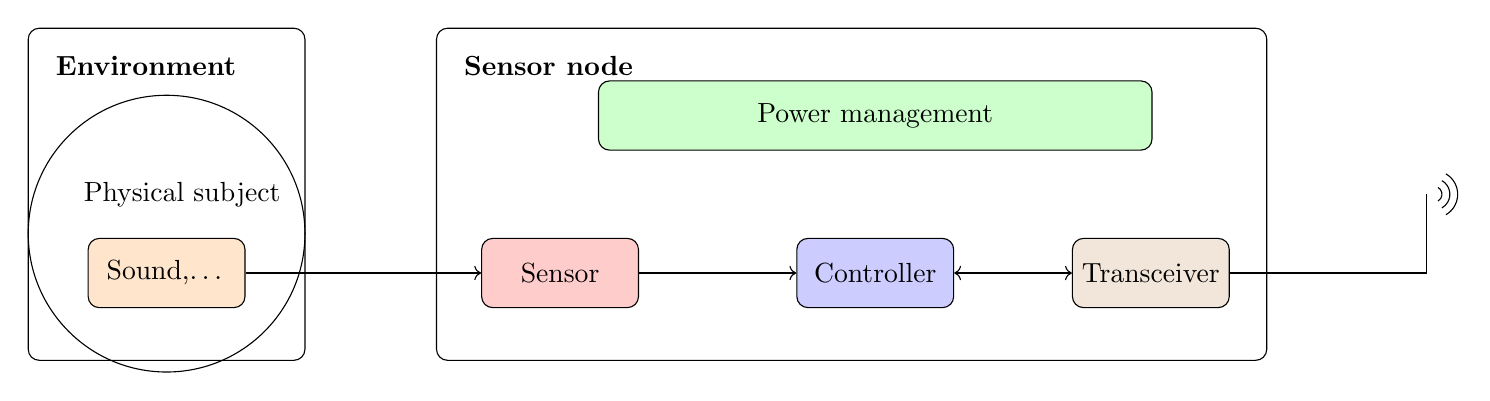
\begin{tikzpicture}
    \node (afe) [afes] {Sensor};
    \path (afe.0)+(-6,0) node (mic) [sensor4] {Sound,\dots};
    \path (afe.0)+(3,0) node (proc) [sensor] {Controller};
    \path (afe.0)+(6.5,0) node (tx) [sensor3] {Transceiver};
    \path (afe.0)+(3,2) node (pw) [sensor2] {Power management};
    \path (afe.0)+(2.7,1) node (mysensor) [empty_block] {};
    \path (afe.0)+(-6,1) node (envi) [empty_block2] {};
    \node[anchor=north west,inner sep=10pt] at (mysensor.north west)
    {\textbf{Sensor node}};
    \draw (afe.0)+(-6,0.5) circle (50pt);
    \node[anchor=north west,inner sep=10pt] at (envi.north west)
    {\textbf{Environment}};
    \path [draw, ->] (mic) -- node [above] {} (afe.west |- mic) ;
    \path [draw, ->] (afe.east) -- node [above] {} (proc.west |- afe) ;
    \path [draw, <->] (proc.east) -- node [above] {} (tx.west |- proc) ;
    \draw (tx.0) -- (11,0) -- (11,1) ;
    \node[] at (-4.8,1) {Physical subject};
    \foreach \r in {.1,.2,.3}
      \draw (11.1,1) ++ (60:\r) arc (60:-60:\r);
\end{tikzpicture}}
\caption{Block diagram of a general IoT sensor node}
\label{fig:general_architecture}
\end{figure}

Because energy is the most important scarcity in such sensors (defining its lifetime), one has to keep in mind the power consumption of each block throughout the design. It is expected that the parts with the most power consumption are the microcontroller, the transceiver and the microphone. The other parts will be designed to be negligible compared to the formers.

\section{Requirements analysis}
\label{section:requirements}

The sensor that will be produced needs to fit the following requirements:

\begin{itemize}
 \item The microphone detects sounds up to \SI{50}{m} in order to produce a reasonable inventory of bird population.
 \item It is able to communicate wirelessly by receiving and transmitting data under power constraints.
 \item Based on the continuously received sound, the sensor has to discriminate the bird species among a small group (4) of selected birds.
 \item The lifetime is one of the most important demands for this application, the sensor has to work fully autonomously (day and night) for at least 15 years.
 \item The materials used for the design, particularly the energy storage element, must have low toxicity.
 \item The device cannot be invasive and should be easy to install. The total volume must not exceed \SI{200 x 200 x 55}{mm} to respect the forest ecosystem and be easily placed on a tree. The main part of the volume will be due to the storage element and the solar cells.
 \item For a massive deployment, the cost cannot exceed 15 euros.
\end{itemize}

%\textcolor{green}{Schema de flow (déroulement du mémoire)}


\chapter{Energy storage}

Energy storage has an important role in sensor applications. First, this role can be identified as either a unique power for the application, or as a temporary storage of energy provided by the energy harvester. In the framework of this thesis, the latter is considered since solar cells (energy harvester) will bring energy to the system, which is stored in an energy storage element.

Then, one has to characterize the main figures of merits such as the energy density, the maximum self-discharge and application conditions, as well as financial and environmental considerations.

A Ragone plot is typically used for comparing the energy density of various energy-storing devices. On such a chart, the values of specific energy density (in \si{Wh/kg}) are plotted versus specific power density (in \si{W/kg}). In Figure~\ref{fig:ragone_plot}, one can see the trade-off between energy density and power density. From fuel cells to supercapacitors by way of Li-ion batteries, energy density is decreasing in aid of power density.

\begin{figure}[H]
    \centering
    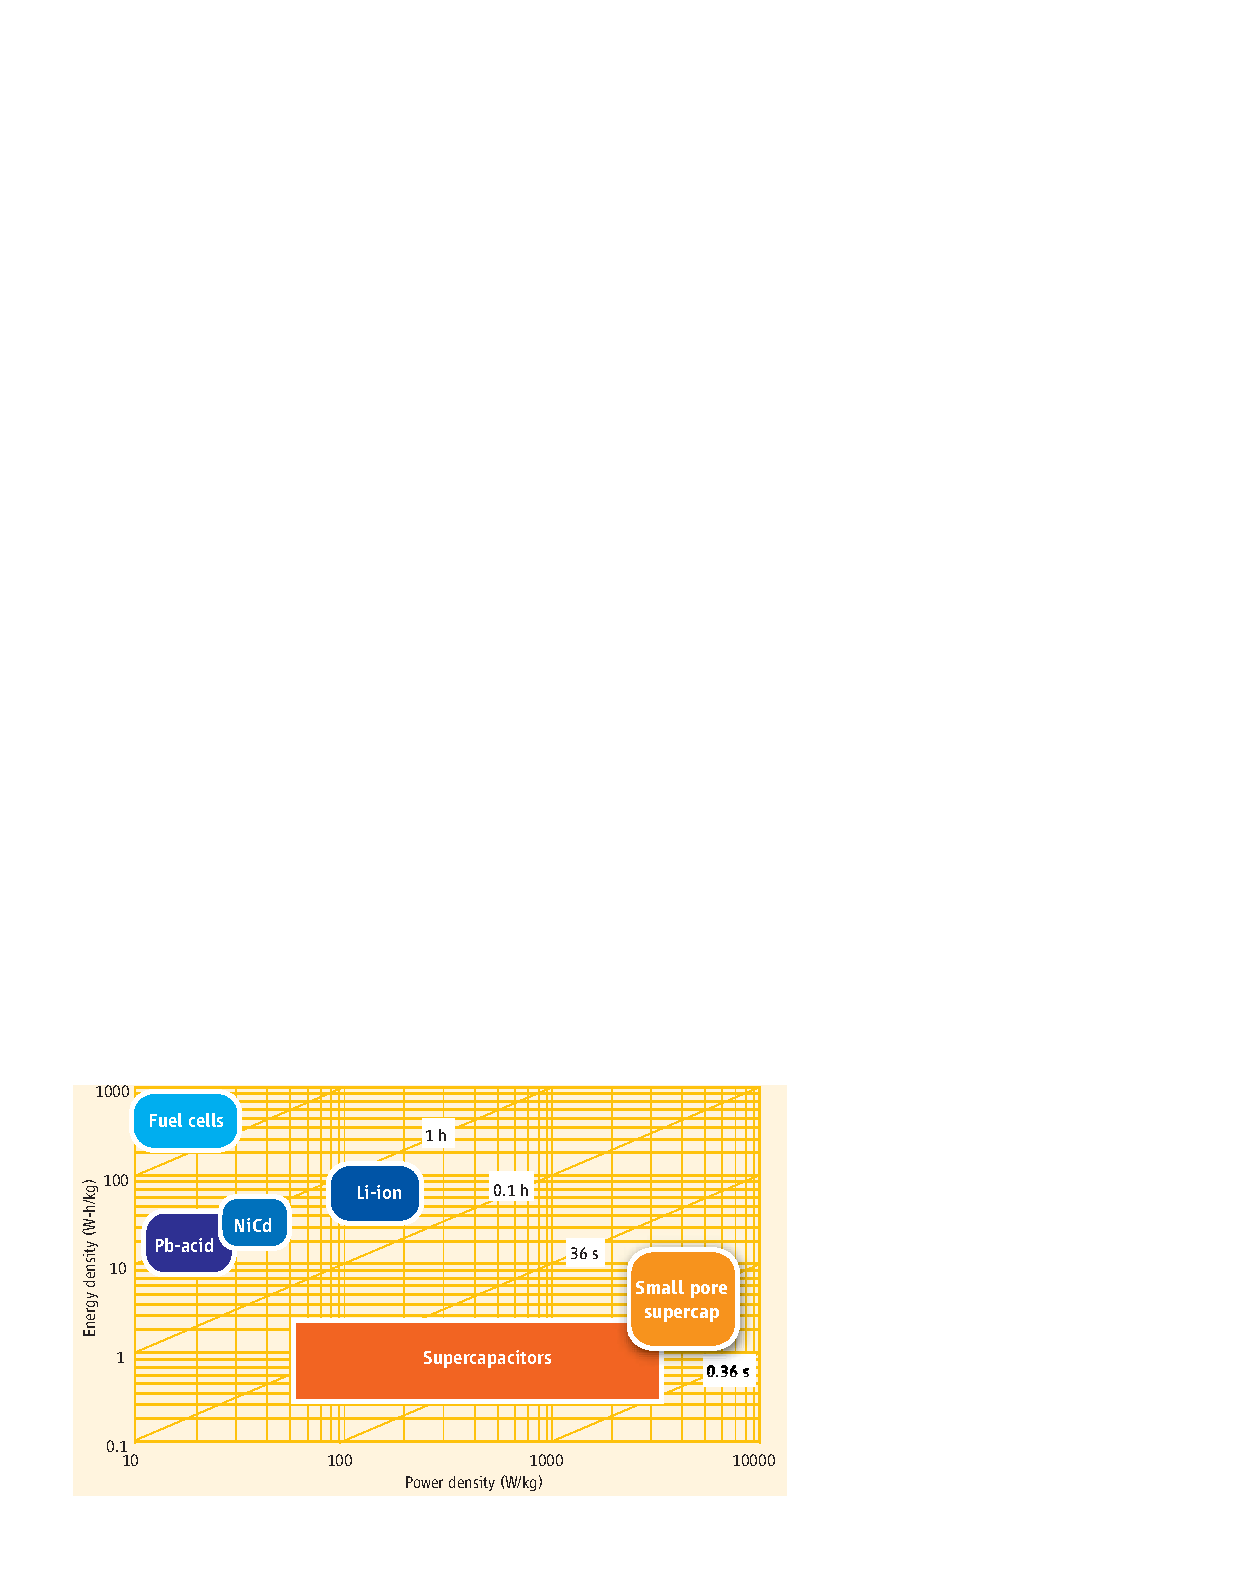
\includegraphics[width=0.8\textwidth]{service2006.pdf}
    \caption[Ragone plot showing specific energy versus specific power for various energy-storing devices]{Ragone plot showing specific energy versus specific power for various energy-storing devices~\cite{Service902}}
    \label{fig:ragone_plot}
\end{figure}

In order to answer the previous requirements, common energy storage types are analyzed and the most suited type for this work is detailed.


\section{Primary batteries}

Primary batteries are non-rechargeable, they thus have only one life cycle. However, they can sometimes still have their place in IoT applications when the power consumption and the sensor lifetime are particularly reduced. Primary batteries are mainly based on three technologies.

\subsection*{Zn-MnO${}_{\textbf{2}}$ batteries}

Zn-MnO${}_2$ batteries are composed of a combination of metallic zinc (oxidation) and a manganese dioxide electrode (reduction). They exist under the form of zinc-carbon cells and alkaline batteries and differ according to the electrolyte inside.

The voltage window is between \SI{0.9}{V} and \SI{1.5}{V}. The energy density of a typical AA (approximately \SI{8}{cm^3}) zinc-carbon cell is \SI{100}{mWh/cm^3}, whereas a commercial alkaline cell reaches at present up to \SI{400}{mWh/cm^3}~\cite{doi:10.1002/er.2949}.

These batteries are very well known and low cost, but present a high self-discharge rate.

\subsection*{Lithium primary batteries}

Lithium primary batteries have an anode made of metallic lithium and a cathode made of several materials such as MnO${}_2$ or FeS${}_2$.

Batteries integrating MnO${}_2$ commonly deliver a total cell voltage of around \SI{3}{V}. These batteries work with the oxidation of lithium and reduction of manganese, with a typical energy density of \SI{650}{mWh/cm^3}.

The second type of lithium battery is based on FeS${}_2$. It has a practical voltage of \SI{1.5}{V} and is therefore compatible with alkaline and zinc-carbon cells. It has an energy density of approximately \SI{550}{mWh/cm^3}.

Overall, it is able to deliver high currents and has a quite flat voltage profile upon discharging. Moreover, it performs well at low temperatures and has a significantly lighter weight than alkaline cells.

\subsection*{Zn-air batteries}

Zn-air batteries are a class of batteries that employ metallic zinc particles as its anode and an aqueous liquid electrolyte. With a voltage of \SI{1.4}{V}, this
battery is commercially available as button cells with an energy density of around \SI{1500}{mWh/cm^3}.

Other disadvantages of this type of battery are that the catalyst that is required for the reduction of oxygen usually consists of expensive noble metals and that the battery is unable to deliver high peak currents. This type of battery is therefore commonly used in applications where only low
currents are required from a battery with a small volume~\cite{doi:10.1002/er.2949}.

\section{Secondary batteries}

Secondary batteries are rechargeable, they thus have a certain number of life cycles (usually more than 500). Only battery types that are suitable for the IoT domain are presented in this thesis.

\subsection*{Batteries with liquid or polymer gel electrolytes}


\subsubsection*{Nickel metal hydride batteries}

Nickel metal hydride batteries (NiMH) combine nickel at the positive electrode and hydrogen (metal hydride) at the negative electrode.  During discharge, a proton, obtained from the electrolyte, occurs in reduction of nickel oxyhydroxide. The loss of protons in the electrolyte produces hydroxide anions which will recombine with a proton from the metal hydride.

The cells typically work at around \SI{1.2}{V}, allowing interchangeability with alkaline batteries. However, they have a higher self-discharge rate and a narrow temperature window (0 to \SI{45}{\degree C}). The energy density is around 250 and \SI{380}{mWh/cm^3}.

\subsubsection*{Li-ion batteries}

Lithium-ion batteries are composed of lithium metal oxide at the positive electrode (LiCoO${}_2$) and a material storing lithium in a neutral form such as graphite at the negative electrode. The charge process is based on the motion of lithium ions from the metal oxide to the electrolyte, where they are stored in graphite.

Compared to NiMH batteries, they have higher energy density (between 300 and \SI{500}{mWh/cm^3}), lower self-discharge rate and larger temperature window (-20 to \SI{60}{\degree C}). They are however easily damaged in case of overdischarging or overcharging, thus requiring a special protective electric circuit for the power management.

Overall, liquid electrolytes (both NiMH and Li-ion) have high volatility and have been the source of explosions in lithium batteries. Research thus has been done on the design of solid electrolytes.

\subsection*{Solid-state batteries}

Solid-state batteries use solid electrodes and a solid electrolyte, such as ceramics (e.g. oxides, sulfides, phosphates) or a solid polymer. They are potentially safer than batteries with liquid electrolytes, with higher energy density, but at a much higher cost.
However, these efforts have faced a number of issues.

One of the biggest problems is that when the battery is charged up, atoms accumulate inside the lithium metal, causing it to expand. These repeated changes in the metal’s dimensions make it difficult for the solids to maintain constant contact, and tend to cause the solid electrolyte to fracture or detach.

Another problem is that none of the proposed solid electrolytes are truly chemically stable while in contact with the highly reactive lithium metal, and they tend to degrade over time.

\section{Supercapacitors}

Supercapacitors are high-capacity capacitors storing energy in an electric field, rather than in a chemical reaction, like batteries. This allows high power density for short-term energy storage\footnote{They can provide very high currents during a short time.}, almost instant recharging and very long lifetimes. Made of porous carbon (electrodes) and liquid salts (electrolyte)~\cite{BAPTISTA20191153}, they are not composed of harmful\footnote{Failing in a nice way, they will never overrun or start a fire.} chemicals or toxic metals.
Since the supercapacitor is non-chemical, the voltage is free to rise until the dielectric fails (often in the form of a short circuit). It is thus needed to avoid going higher than the specified voltage, which is characterized by a lower voltage limit than for batteries.

Due to their behavior in between electrolytic capacitors and batteries, they are particularly well suited for IoT applications. Indeed, they typically store 10 to 100 times more energy per unit volume or mass than electrolytic capacitors. They can also accept and deliver charge much faster than batteries, and tolerate many more charge and discharge cycles than rechargeable batteries. Nevertheless, care needs to be paid to their significant leakage current which is proportional to the capacitance of the supercapacitor.

Instead of using a conventional solid dielectric, supercapacitors use electrostatic double-layer capacitance and electrochemical pseudocapacitance~\cite{2019JPS...414..420B}.

\subsection*{Electrostatic double-layer capacitors}

Electrostatic double-layer capacitors (EDLCs) are the most common type of supercapacitors. They use carbon electrodes or derivatives with much higher electrostatic double-layer capacitance than electrochemical pseudocapacitance, achieving separation of charge in a Helmholtz double layer at the interface between the surface of a conductive electrode and an electrolyte.

\subsection*{Electrochemical pseudocapacitors}

Electrochemical pseudocapacitors use metal oxide or conducting polymer electrodes with a high amount of electrochemical pseudocapacitance additional to the double-layer capacitance. They store charge chemically through redox reactions where one species transfers electrons to another, similar to a battery. While pseudocapacitors store more energy, their widespread use has been hampered by their narrow electrochemical voltage window, which is the voltage range where the electrode materials are stable.

Additionally, there exist hybrid capacitors, such as the lithium-ion capacitors, using electrodes with different characteristics: one exhibiting mostly electrostatic capacitance and the other mostly electrochemical capacitance.

\section{New developments}

Promising new methods are also developed in research laboratories, some of them are detailed hereafter.

\subsection*{3D electrodes for electrochemical energy storage}

Superior energy or power density for batteries is typically achieved only in ultra-thin electrodes with low mass loadings. To realize the full potential of these electrode materials, new electrode architectures allow more efficient charge transport beyond the limits of traditional electrodes. Working on the design and synthesis of 3D electrodes is promising to address charge transport limitations in thick electrodes. Such 3D porous architectures could enable composite electrodes with an unprecedented combination of energy and power densities~\cite{Sun2019}.

In addition to the recent development of Li-ion batteries with  flexible, bendable, or foldable characteristics, some research has been focused on batteries with advanced features of stretchability in which the systems are able to accommodate large mechanical strain and still maintain their functions. Such sponge-inspired electrodes for stretchable Li-ion batteries show no specific capacity reduction when bent, unlike the cells using conventional electrodes~\cite{doi:10.1002/adma.201505299}.

\subsection*{Lithium metal anode}

Recent research has been achieved on lithium metal anodes that could improve the longevity and energy density of future batteries~\cite{10.1038/s41586-020-1972-y}.

Most attempts to overcome the problems of solid-state batteries have focused on designing solid electrolyte materials that are absolutely stable against lithium metal, which turns out to be difficult.  Instead, some researchers adopted an unusual design that utilizes two additional classes of solids, ``mixed ionic-electronic conductors'' (MIEC) and “electron and Li-ion insulators” (ELI), which are absolutely chemically stable in contact with lithium metal. 

They developed a three-dimensional nanoarchitecture in the form of a honeycomb-like array of hexagonal MIEC tubes, partially infused with the solid lithium metal to form one electrode of the battery, but with extra space left inside each tube. When the lithium expands in the charging process, it flows into the empty space in the interior of the tubes, moving like a liquid even though it retains its solid crystalline structure. This flow, entirely confined inside the honeycomb structure, relieves the pressure from the expansion caused by charging, but without changing the outer dimensions of the electrode or the boundary between the electrode and electrolyte. The other material, the ELI, serves as a crucial mechanical binder between the MIEC walls and the solid electrolyte layer.

\section{Shape}

In addition to the electrical and thermal characteristics, the form of the storage element is particularly important for IoT devices where the full sensor size is often limited. The main trade-off thus appears between the charge capacity and the size of the energy storage element.

The main shapes of micro-batteries are button cells, pouch cells and thin film batteries.

\section{Comparison}

Table~\ref{tab:comparison_energy_storage} presents the main figures of merit for the previously described types of energy storage.

\begin{table}[H]
\centering
\scalebox{0.655}{
\begin{tabular}{l|ccc|ccc}
\toprule
                          & \multicolumn{3}{c|}{Capacitors} & \multicolumn{3}{c}{Batteries} \\ \midrule
                          & Ceramic & Electrolytic & Supercap & Non-rechargeable & \multicolumn{2}{c}{Rechargeable} \\
                          &  &  & EDLC & Alkaline & NiMH & Lithium ion \\ \midrule
 Power density [W/g]      &  & > 100 & 2 -- 10 &  & 2.5 -- 10 & 1 -- 3  \\
 Energy density [mWh/g]   & 0.1~\cite{DEKIMPE20198} & 0.01 -- 0.3  & 5 &  & 60 -- 120  & 120 -- 240 \\
 Self-discharge rate [per month]     & 100\% & \SI{100}{h} & 50\% & < 0.3\% & 0.08 – 2.9\% & 5\% \\
 Leakage current          & 1 -- 100 \si{nA/\micro F}  &  & 2 -- 5 \si{fA/\micro F}~\cite{DMF3Z5R5H474M3DTA0}~\cite{Vishay} &  &  & 5 \si{\micro A}~\cite{DEKIMPE20198} \\
 Service life [years]     & 25~\cite{DEKIMPE20198} & 15 & 10 -- 15 & 5 -- 10 &  & 5 --10 \\
 Life cycles              & unlimited~\cite{DEKIMPE20198} & unlimited & \SI{1000000}{} & 1 & 180 -- 2000 & 500 \\
 Degradation              & negligible &  & -80\% in 10 years &    &  & -50\% in 500 cycles     \\
 Charge time              &    &  & 1 -- \SI{10}{s} &    &  & 10 -- \SI{60}{min}     \\
 Cell voltage [V]             &    & 4 -- 630 & 2.3 -- 2.75 & 1.5   & 1.2 & 3.6     \\
 Charge T° [\si{\degree C}] &  & -40 -- 70 & -40 -- 65 & & & 0 -- 45 \\
 Discharge T° [\si{\degree C}]             &  & -40 -- 70 & -40 -- 65 & & & -20 -- 60 \\
 Discharge efficiency     &   & 99\% & 95\% &    & 66\% -- 92\% & 90\%     \\
 Toxicity                 &    &  & low &    &  & middle \\ \bottomrule
\end{tabular}
}
\caption{Comparison of various types of energy storage}
\label{tab:comparison_energy_storage}
\end{table}

In this table, the life cycle is the number of complete charge/discharge cycles that the battery is able to support before its capacity falls under 80\% of its original capacity.
Although the deployment of such sensors would imply the fabrication of several thousands of energy storage elements, the impact of the toxicity is small for such projects lasting more than 20 years without replacement. The degradation corresponds to the decrease of its maximum energy storage throughout its life.

Another factor of merit is the overall efficiency, which is computed as
\[
 \eta = \frac{E_\te{O}}{E_\te{I}}
\]
where $E_\te{O}$ is the energy delivered during the whole life of the energy storage element, and $E_\te{I}$ is the total energy fed to the storage element, composed of both the fabrication energy and the recharge energy. It is difficult to compute this efficiency due to the lack of information about the fabrication energy (typically not given by manufacturers). However, Li-ion batteries (\SI{50.17}{kWh/kg} for electric vehicles~\cite{manufacturing_lithium}) generally require more manufacturing energy than supercapacitors.


\subsection*{Criticality}

To assess the criticality of energy storage elements, one needs to consider the environmental and societal impacts combined with their scarcity. The scarcity of an element is assessed by the variation of its availability on Earth between the past decades and nowadays (not to be confused with rare-earth elements which are not critical). They include components overused for electronic devices such as copper, gold, silver, lithium and cobalt.

For Lithium-ion and NiMH batteries, the following compounds are used:
\begin{itemize}
 \item Positive electrode: metal oxide compounds such as lithium extracted from brine or rock, nickel, cobalt, hydrogen-absorbing alloy (nickel alloys with many metals: V, Ti, Zr, Ni, Cr, Co, Al and Fe)
 \item Negative electrode: graphite (carbon-based)
 \item Electrolyte
\end{itemize}

One can thus see that many critical and polluting compounds appear in the positive electrode.

For EDLCs, the following compounds are used:

\begin{itemize}
 \item Electrodes: porous carbon (activated carbon, carbon nanotubes and carbon aerogels) built from graphite \cite{Hastak}
 \item Electrolyte: liquid salts (water with ions)
 \item Polymeric membrane forming a microporous layer as separator
\end{itemize}

Supercapacitors are thus mainly built from carbon, one of the most abundant elements on Earth. They are far less toxic and resource-intensive than metal-based batteries.

    
\section{Selection}

Building upon these results, a supercapacitor is chosen because of its high lifetime, low toxicity, low criticality and reasonable energy density. As detailed in the Ragone plot (Figure~\ref{fig:ragone_plot}), this energy storage element can deliver high currents but stores less energy per volume. Its substantial leakage current is also needed to be further taken care of. The sizing of this supercapacitor will be achieved in Chapter~\ref{supercap_sizing} once the whole power consumption is fully determined. 

%Approx energy available based on normal volume of supercap -> guideline through the design -> compared with this value and check that small parts draw less than 1 percent of this energy.

\chapter{Power management}

The purpose of power management is to harvest energy from solar cells, store it in a supercapacitor, and deliver it to the circuit through a stable voltage supply. In this section, the best supply voltage is determined and the power management unit is explained.

\section{Operating voltage design}
\label{section:operating_voltage}

First, the supply voltage is used to power the sensing subsystem and the MCU/transceiver chip. For practical and energy efficiency reasons, the same supply voltage is selected for the whole system.

Since the microcontroller uses a low-dropout (LDO) regulator to regulate its internal voltage, the current consumption is independent from the supply voltage. In order to minimize the power consumption, one thus needs to use the lowest supply voltage. However, using a low supply voltage decreases the AFE amplification gain and therefore the precision (i.e. the signal-to-noise ratio) on the microphone signal that will be read at the input of the MCU. Indeed, while the noise at the sensing output is roughly independent from the amplification gain of the sensing subsystem (see the proof in Section~\ref{section:AFE}), the signal power is reduced with the gain. Hence, this trade-off leads to the selection of a \SI{2.5}{V} supply voltage which lies in the \SI{2.2}{V} -- \SI{3.6}{V} range of the CMWX1ZZABZ chip.

%the resolution of an $N$-bit ADC is given by $V_\te{DD}/2^N$ where $V_\te{DD}$ is the supply voltage.


\section{Power management unit}
\label{section:PMU}

A power management unit (PMU) is an integrated energy management circuit that extracts DC power from solar cells to simultaneously store energy in a rechargeable element and supply the system with independent regulated voltages. An AEM10941 chip from e-peas is selected because of its ultra-low power consumption and the close relations between the university and the company (see Figure~\ref{fig:AEM10941}).

\begin{figure}[H]
    \centering
    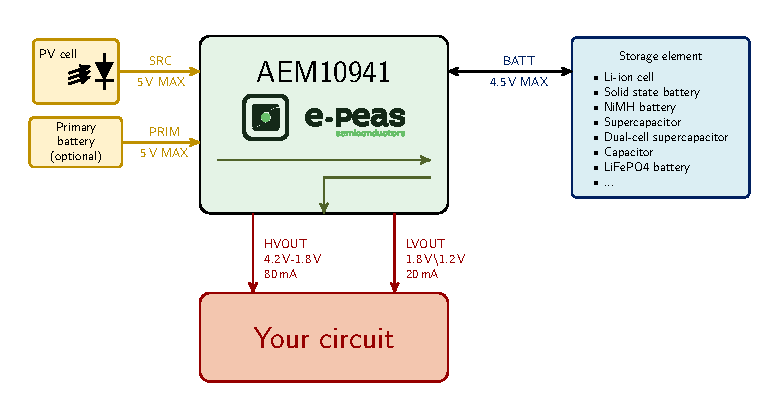
\includegraphics[width=0.7\textwidth]{AEM10941.pdf}
    \caption[AEM10941 simplified schematic view]{AEM10941 simplified schematic view~\cite{AEM10941}}
    \label{fig:AEM10941}
\end{figure}

Its characteristics are given in Table~\ref{tab:AEM10941}, by only considering the high voltage regulator. The very low quiescent current is nearly independent from the supercapacitor voltage.

\begin{table}[H]
\centering
\scalebox{1}{
\begin{tabular}{lc}
\toprule
 Max input current                       & \SI{110}{mA}               \\
 Max input voltage                       & \SI{5}{V}                  \\
 Output voltage                          & \SI{1.8}{V} -- \SI{4.1}{V} \\
 Max output current                      & \SI{80}{mA}                \\
 Max supercap charge                     & \SI{4.5}{V}                \\ 
 Min dropout supercap -- output voltage & \SI{0.3}{V}                \\ 
 Quiescent current                       & \SI{0.6}{\micro A}         \\ \bottomrule
\end{tabular}
}
\caption{Characteristics of the AEM10941 PMU}
\label{tab:AEM10941}
\end{table}


\subsection*{Storage element and LDO configuration}

Configuration pins determine various operating modes by setting predefined conditions for the energy storage element (overcharge or overdischarge voltages) and by selecting the voltage of the high-voltage supply and the low-voltage supply.
The low-voltage supply is not used and the high-voltage supply is set to \SI{2.5}{V}. These characteristics correspond to a preset state in the chip, which helps reduce internal losses by not using additional resistors to select a custom configuration. The three configuration pins CFG[2], CFG[1] and CFG[0] are thus set to 0, 1 and 1, corresponding to the charge of a dual-cell supercapacitor charged in the range \SI{2.8}{V} -- \SI{4.5}{V} in order to power the low-voltage and high-voltage supplies at \SI{1.8}{V} and \SI{2.5}{V}, respectively.

Additionally, three status pins allow monitoring the PMU, whose one informs about supercapacitor overdischarge. For a first prototype, connecting this pin to a LED can be useful to deduce the supercapacitor state, but it is not used in the final model to further reduce power consumption (which is non-negligible for typical LEDs, around \SI{1}{mA}).

\subsection*{Maximum power point tracking}

The efficiency of power transfer from the solar cell depends on both the amount of sunlight arriving on the solar cells and the electrical characteristics of the load. As the amount of sunlight varies, the load characteristic that produces the highest power transfer efficiency changes, so that the efficiency of the system is optimized when the load characteristic changes to keep the power transfer at highest efficiency. 
Maximum power point tracking (MPPT) is thus used by the PMU by means of a boost converter regulating its input voltage so that the electrical current that enters the boost converter yields the best power transfer from the harvester under any ambient conditions (see Section~\ref{section:solar_cells} for more details about the intrinsic principle of solar cells).

This PMU uses the open-circuit voltage algorithm, the simplest MPPT control method. It consists to set the voltage at a constant ratio of the open-circuit voltage $V_\te{OC}$. By temporarily disconnecting the source from the PMU, the MPPT module maintains knowledge of $V_\te{OC}$. It then sets the MPPT voltage at $V_\te{MPPT}$ depending on $V_\te{OC}$ and the ratio (70\%, 75\%, 85\% or 90\%) selected in hardware via two headers connected to the configuration pins. A typical MPPT ratio leading to the maximum power is 76\%~\cite{10.1109/ICSTE.2010.5608868}, but it will be refined experimentally in the validation section. Still, the main disadvantage of this method is that there is momentary power loss due to the disconnection of the load from the solar cells for the sampling of its open-circuit voltage.


\subsection*{Boost conversion efficiency}

The energy converted from the solar cells to the supercapacitor (called boost voltage) is not fully converted due to the internal boost converter efficiency. As depicted in Figure~\ref{fig:boost_efficiency} for a typical harvested current of \SI{10}{mA}, the efficiency is maximum when the input voltage $V_\te{SRC}$ is \SI{0.4}{V} below the output voltage $V_\te{BOOST}$ (see Table~\ref{tab:max_eff_PMU}).

\begin{figure}[H]
    \centering
    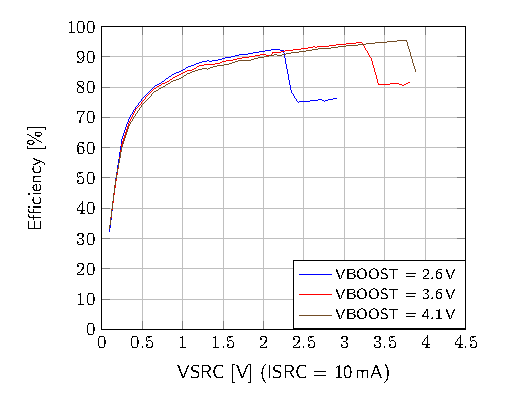
\includegraphics[width=0.6\textwidth]{boost_efficiency.pdf}
    \caption{Boost conversion efficiency (solar cells -- supercap) of the AEM10941}
    \label{fig:boost_efficiency}
\end{figure}

\begin{table}[H]
\centering
\begin{tabular}{ccc}
\toprule
 $V_\te{SRC}$ & $V_\te{BOOST}$ & Efficiency \\ \midrule
 \SI{2.2}{V}  & \SI{2.6}{V}    & 92\%      \\
 \SI{3.2}{V}  & \SI{3.6}{V}    & 95\%      \\
 \SI{3.7}{V}  & \SI{4.1}{V}    & 96\%      \\ \bottomrule
\end{tabular}
\caption{Values of maximum efficiency for the src -- boost conversion with a \SI{10}{mA} input current}
\label{tab:max_eff_PMU}
\end{table}

Since the source voltage impacts both the boost conversion efficiency and the harvested power (see previous paragraph), the optimal source voltage needs to be determined. Based on Figure~\ref{fig:boost_efficiency}, the efficiency significantly falls when the source voltage exceeds its optimal voltage. The source voltage thus needs to stay below $V_\te{BOOST} - \SI{0.4}{V}$ at all times, corresponding to \SI{2.4}{V} for this work (supply voltage of \SI{2.5}{V} implying a supercap voltage of at least \SI{2.8}{V}). In this case, it is thus expected to reach a boost efficiency of 92\% whatever the supercap voltage. Finally, the maximum source voltage set to \SI{2.4}{V} might be slightly relaxed if the IV curve of the solar cells provide a significant power increase at a higher source voltage (see Section~\ref{section:solar_cells}).


\subsection*{High-voltage LDO regulation}

As shown in Figure~\ref{fig:LDO_voltage}, the PMU supply voltage depends on the load current drawn by the sensing and MCU/RF subsystems. It decreases from \SI{2.5}{V} without load to \SI{2.43}{V} at the maximum load (that is, \SI{80}{mA}). Although this voltage variation might impinge upon the signal reading at the ADC input of the microcontroller, no voltage regulation needs to be taken into account inside the MCU code. Indeed, both the signal voltage $V_\te{in,ADC}$ from the microphone and the ADC supply voltage $V_\te{DD}$ vary likewise, this leads to the same digitized number $\floor{V_\te{in,ADC}/V_\te{DD}}$.

\begin{figure}[H]
    \centering
    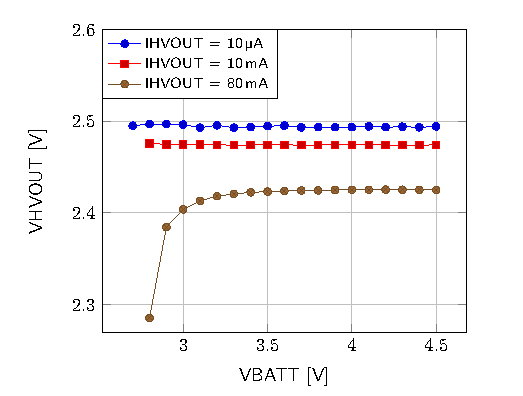
\includegraphics[width=0.6\textwidth]{LDO_voltage.pdf}
    \caption{High-voltage LDO regulation at \SI{2.5}{V} in function of the load current}
    \label{fig:LDO_voltage}
\end{figure}

Finally, the LDO efficiency can be simply calculated as $V_\te{out}/V_\te{in}$ (same input -- output current) if the quiescent current (\SI{0.6}{\micro A}) can be neglected with regards to the output current. The hyperbolic curve in Figure~\ref{fig:LDO_efficiency} confirms the $1/V_\te{in}$ dependence of the efficiency on $V_\te{in}$. It is thus advised to work at the lowest supercap voltage (i.e. \SI{2.8}{V}) by selecting a supercapacitor with a similar operation voltage range.

\begin{figure}[H]
    \centering
    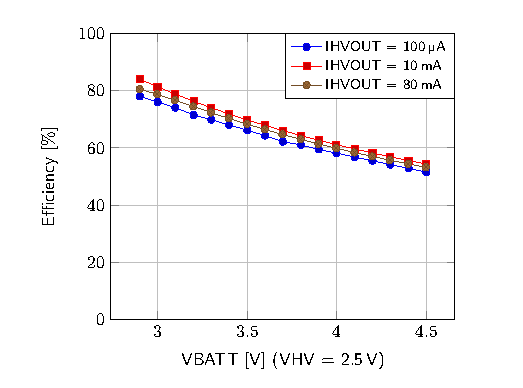
\includegraphics[width=0.6\textwidth]{LDO_efficiency.pdf}
    \caption{High-voltage LDO efficiency at \SI{2.5}{V} in function of the load current}
    \label{fig:LDO_efficiency}
\end{figure}


\chapter{Sensing subsystem}

Sound waves are generated by the variation of a physical characteristic, the pressure. This deviation propagates via vibrations in the environment in such a way that sound can be measured by a microphone from a distance of the source.

Sound waves are often described in terms of sinusoidal plane waves (see Figure~\ref{fig:sound_wave}). Hence, they have a direction of propagation, a speed $v$, a frequency $f$ and an amplitude $A$. 

\begin{figure}[H]
\centering
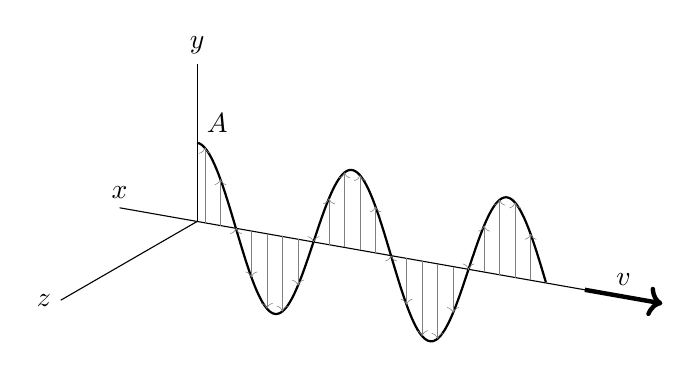
\begin{tikzpicture}[x={(-10:1cm)},y={(90:1cm)},z={(210:1cm)}]
    % Axes
    \draw (-1,0,0) node[above] {$x$} -- (5,0,0);
    \draw (0,0,0) -- (0,2,0) node[above] {$y$};
    \draw (0,0,0) -- (0,0,2) node[left] {$z$};
    % Propagation
    \draw[->,ultra thick] (5,0,0) -- node[above] {$v$} (6,0,0);
    % Waves
    \draw[thick] plot[domain=0:4.5,samples=200] (\x,{cos(deg(pi*\x))},0);
    % Arrows
    \foreach \x in {0.1,0.3,...,4.4} {
        \draw[->,help lines] (\x,0,0) -- (\x,{cos(deg(pi*\x))},0);
    }
    % Labels
    \node[above right] at (0,1,0) {$A$};
    \node[below] at (0,0,1) {};
\end{tikzpicture}
\caption{General sound wave description}
\label{fig:sound_wave}
\end{figure}

The amplitude of sound pressure corresponds to the loudness of a sound and is typically expressed as the root mean square (RMS) amplitude, called sound
pressure level (SPL). Let the RMS sound pressure be $p=A/\sqrt{2}$ for sine waves, the SPL amplitude is given by
\[
 L_p = 20\log_{10}\left(\frac{p}{p_0}\right) \simeq 20\log_{10}(p) + 94 \quad [\si{dB_{SPL}}]
\]
where $p_0=\SI{20}{\micro Pa}$ is the reference RMS pressure (hearing threshold of humans at \SI{1}{kHz}).

Additionally, the sound SPL amplitude changes over the distance (from $r_1$ to $r_2$) according to the propagation law of spherical waves:
\[
 L_{p_2} = L_{p_1} + 20\log_{10}\left(\frac{r_2}{r_1}\right) \quad [\si{dB_{SPL}}].
\]

Table~\ref{tab:sound_levels} gives typical sound pressure levels.

\begin{table}[H]
\centering
\scalebox{1}{
\begin{tabular}{lcc}
\toprule
  Source of sound & Distance & Sound pressure [dB] \\ \midrule
  Jet engine           & \SI{1}{m}   & 150 \\
  Trumpet              & \SI{0.5}{m} & 120 \\
  Traffic on busy road & \SI{10}{m}  & 90  \\
  Passenger car        & \SI{10}{m}  & 70  \\
  Quiet room           & ambient     & 25  \\ \bottomrule
\end{tabular}
}
\caption{Typical sound pressure levels}
\label{tab:sound_levels}
\end{table}

In this work, the sensor is required to detect the song of a bird (around \SI{50}{dB_{SPL}} at \SI{1}{m} of the source) located \SI{50}{m} away. The minimum detected sound pressure is thus
\[
 L_{p_\te{min}} = 50 - 20\log_{10}(50) = \SI{16}{dB_{SPL}}.
\]
Sound production from several bird species have been measured up to \SI{95}{dB_{SPL}} and are generally greater for larger birds~\cite{FHWA}. The sensor thus needs to detect sounds of at least
\[
 L_{p_\te{max}} = 95 - 20\log_{10}(50) = \SI{61}{dB_{SPL}}.
\]

The frequency range of human hearing is often reported to be between 20 and \SI{20000}{Hz}, but the ability to hear higher frequencies decreases with age. For this reason, a correction, called A-weighting, is applied to instrument-measured sound levels to account for the relative loudness perceived by the human ear as a function of the frequency (see Figure~\ref{fig:a_weighting}).

\begin{figure}[H]
    \centering
    % This file was created by matlab2tikz.
%
%The latest updates can be retrieved from
%  http://www.mathworks.com/matlabcentral/fileexchange/22022-matlab2tikz-matlab2tikz
%where you can also make suggestions and rate matlab2tikz.
%
\definecolor{mycolor1}{rgb}{0.00000,0.44700,0.74100}%
%
\begin{tikzpicture}

\begin{axis}[%
width=4.521in,
height=3.566in,
at={(0.758in,0.481in)},
scale only axis,
xmode=log,
xmin=10,
xmax=100000,
xminorticks=true,
xlabel style={font=\color{white!15!black}},
xlabel={Frequency [Hz]},
ymin=-60,
ymax=10,
ylabel style={font=\color{white!15!black}},
ylabel={Gain [dB]},
axis background/.style={fill=white},
xmajorgrids,
xminorgrids,
ymajorgrids
]
\addplot [color=mycolor1, forget plot]
  table[row sep=crcr]{%
20	-50.3946568854394\\
21.4453444402065	-48.6018111353701\\
22.9951399079547	-46.8543294397198\\
24.6569347888413	-45.1522093541212\\
26.4388229693206	-43.4951117397424\\
28.3494832585361	-41.882396156046\\
30.3982216590587	-40.3131678182811\\
32.5950166924129	-38.7863327592259\\
34.9505680001537	-37.3006574124414\\
37.4763484572077	-35.8548287938306\\
40.1846600513009	-34.4475117487002\\
43.0886938006377	-33.0774002648038\\
46.2025940016632	-31.7432605273971\\
49.5415271198342	-30.4439641184671\\
53.1217556589337	-29.1785104706293\\
56.960717368716	-27.9460383368323\\
61.0771101766683	-26.7458266158705\\
65.4909832575546	-25.5772853839389\\
70.2238346843026	-24.4399384335685\\
75.2987161358494	-23.3333990184921\\
80.7403451719311	-22.257340839654\\
86.5752256216612	-21.2114665623196\\
92.8317766722556	-20.1954762938146\\
99.5404712866422	-19.2090384389653\\
106.733984624126	-18.2517651571547\\
114.447353187004	-17.3231942626694\\
122.718145468264	-16.4227788591714\\
131.586644931514	-15.5498853305849\\
141.096046214373	-14.7037995990206\\
151.292665510926	-13.8837408900169\\
162.226166157937	-13.088881693576\\
173.949800523557	-12.3183722309625\\
186.520669376644	-11.571367554977\\
200	-10.8470554155775\\
214.453444402065	-10.1446831770816\\
229.951399079547	-9.46358232639582\\
246.569347888413	-8.80318940973537\\
264.388229693206	-8.16306253185792\\
283.494832585361	-7.54289281519858\\
303.982216590587	-6.94251043182442\\
325.950166924129	-6.36188499031939\\
349.505680001537	-5.80112019677372\\
374.763484572077	-5.26044283607855\\
401.846600513009	-4.74018626122914\\
430.886938006377	-4.24076875562261\\
462.025940016632	-3.76266735909994\\
495.415271198342	-3.30638802217176\\
531.217556589337	-2.87243325758999\\
569.60717368716	-2.4612687605029\\
610.771101766683	-2.07329072063633\\
654.909832575546	-1.70879569893254\\
702.238346843026	-1.36795493835872\\
752.987161358494	-1.05079479298957\\
807.403451719311	-0.757184587780772\\
865.752256216612	-0.486832693781293\\
928.317766722557	-0.239290980711657\\
995.404712866423	-0.0139671717433858\\
1067.33984624126	0.189855941390674\\
1144.47353187004	0.372995890080746\\
1227.18145468264	0.53634223432847\\
1315.86644931514	0.680826333016177\\
1410.96046214373	0.807390798829371\\
1512.92665510926	0.91695999521274\\
1622.26166157937	1.01041259360507\\
1739.49800523557	1.08855684772189\\
1865.20669376644	1.15210890309468\\
2000	1.20167417607769\\
2144.53444402065	1.23773162439113\\
2299.51399079547	1.26062059593529\\
2465.69347888413	1.27052988012526\\
2643.88229693206	1.26748858715904\\
2834.94832585361	1.25135853410571\\
3039.82216590587	1.22182791118249\\
3259.50166924129	1.17840612695505\\
3495.05680001537	1.12041987873726\\
3747.63484572077	1.04701065643129\\
4018.4660051301	0.957134056676506\\
4308.86938006377	0.849561450467641\\
4620.25940016632	0.722884699823357\\
4954.15271198342	0.57552474246588\\
5312.17556589337	0.405744938416924\\
5696.07173687161	0.21167007563824\\
6107.71101766683	-0.00868816215263468\\
6549.09832575546	-0.257398677863686\\
7022.38346843026	-0.536571160732572\\
7529.87161358494	-0.848309268789694\\
8074.03451719311	-1.19465768481864\\
8657.52256216612	-1.57754464532247\\
9283.17766722556	-1.99872226155299\\
9954.04712866422	-2.45970758439648\\
10673.3984624126	-2.96172780068734\\
11444.7353187004	-3.50567308455211\\
12271.8145468264	-4.09206039226472\\
13158.6644931514	-4.72101086482632\\
14109.6046214373	-5.39224253728376\\
15129.2665510926	-6.10507885998396\\
16222.6166157937	-6.85847227237928\\
17394.9800523557	-7.65104090697224\\
18652.0669376644	-8.4811155911372\\
20000	-9.34679375948158\\
};
\end{axis}
\end{tikzpicture}%
    \caption{A-weighting curve}
    \label{fig:a_weighting}
\end{figure}

Many bird songs have frequency ranges between \SI{1}{kHz} and \SI{8}{kHz}, which places them in the spot of human hearing. However, some birds can produce sounds at frequencies\footnote{One might also want to assess the impact of moving birds on the frequency. For this purpose, the Doppler effect characterizes the frequency $f$ perceived at the sensor node compared to the emitted frequency $f_s$ of the bird when it moves at speed $v_s$. The relative variation of frequency is given by $ f/f_0 = \frac{v}{v \pm v_\text{s}}$ where $v$ is the sound velocity (\SI{343}{m/s} in ambient conditions). For a typical bird velocity (\SI{12}{m/s}), the equation provides a relative variation of $\pm \SI{4}{\%}$, which corresponds to a small (but non-negligible) impact on the perceived frequency.} as low as \SI{23}{Hz}~\cite{10.2307/4090277} or as high as \SI{15}{kHz}~\cite{doi:10.1111/j.1474-919X.1962.tb08647.x}. Since the presented sensor aims to mainly analyze bird sounds, it has to match the frequency specifications ranging between \SI{20}{Hz} and \SI{20}{kHz}.

In the end, the characteristics of the sound wave at the sensor are summed up in Table~\ref{tab:wave_charact_sensor}.

\begin{table}[H]
\centering
\scalebox{1}{
\begin{tabular}{lcc}
\toprule
  Pressure range & 16 -- 61 & \si{dB_{SPL}} \\
  Frequency range  & 20 -- 20000 &  Hz      \\ \bottomrule
\end{tabular}
}
\caption{Sound wave characteristics at the sensor}
\label{tab:wave_charact_sensor}
\end{table}


As depicted in Figure~\ref{fig:sensing_subsystem}, the sensing subsystem is composed of a microphone and a signal conditioning circuit called analog front-end. This block handles the signal transmission from the input sound pressure detected by the microphone to an analog voltage $V_{\te{mic,ADC}}$ further processed by a microcontroller.

\begin{figure}[H]
\centering
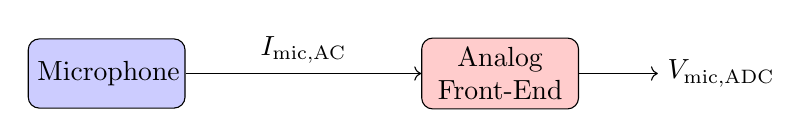
\begin{tikzpicture}
    \node (afe) [afes] {Analog Front-End};
    \path (afe.0)+(-6,0) node (mic) [sensor] {Microphone};
    \path [draw, ->] (mic) -- node [above] {$I_{\te{mic,AC}}$} (afe.west |- mic) ;
    \draw [->] (afe.0) -- node [ann] {} + (1,0) node[right] {$V_{\te{mic,ADC}}$};
\end{tikzpicture}
\caption{Block diagram of the sensing subsystem}
\label{fig:sensing_subsystem}
\end{figure}

\section{Microphone}

A microphone is a device that converts sound into an electrical signal (also called transducer). Generally, they mimic the inner workings of human ear by using a diaphragm which vibrates with the sound pressure. There exist several types of microphones for which the most important characteristics, called figures of merit, need to be compared.


\subsection*{Main types of microphone}

Microphones are categorized by their transducer principle, corresponding to the way they detect the variation of input sound pressure.

\subsubsection*{Carbon microphones}

Carbon microphones were the first created type of electrical microphone. They are based on the variation of electrical resistance between two plates due to the motion of a diaphragm on one of these plates. This type of microphone is less used because of its limited frequency response and high noise level (background and crackling noise~\cite{background.noise}).

\subsubsection*{Optical microphones}

Optical microphones use the moving diaphragm as a reflection plate for the light of a laser. The intensity of the light, depending on the deformation of the diaphragm, is converted to an electrical signal through a photodiode. Their high power consumption (more than \SI{5}{mW}, \SI{5.4}{mW} in~\cite{optical_microphone})  prevents them from being used in IoT applications.

\subsubsection*{Condenser microphones}

Condenser microphones are based on a parallel-plate capacitor for which one of the plates is the diagram. For a fixed charge $Q$ on the capacitor, the voltage across the capacitor varies with the capacitance according to
\[
V = \frac{Qd}{\varepsilon A}
\]
where $s$ is the distance between the plates, $A$ is the area of the plate, and $\varepsilon$ is the electric permittivity of the medium inside the plates.

This type can be further divided in active and passive condenser microphones.

Active condenser microphones require biasing circuitry to charge the capacitor and perform first stage amplification. In this group belong microelectromechanical systems (MEMS) microphones which are small package condenser microphones made using semiconductor production techniques. Typically, they already integrate an ADC inside. The small size and the rather low power consumption (\SI{10}{\micro W} to  \SI{1}{mW}~\cite{ICS40720},~\cite{10.3390/mi9070323}) of MEMS microphones are ideal for IoT applications.
 
Passive condenser microphones do not require biasing of the capacitor. For instance, condenser electret microphones have an electret material as diaphragm, a material that has a permanent electrical charge on it. Passive microphones are also appealing for their low power consumption and reduced complexity.
 
\subsubsection*{Piezoelectric microphones}

Piezoelectric microphones directly translate the sound pressure into a voltage by means of a piezoelectric crystal, which redistributes the charges in the crystal under a deformation. They can be packaged in MEMS microphones and have a low power consumption (about \SI{300}{\micro W}~\cite{PMM-3738-VM1000-R}). However, their high impedance makes them sensitive to electrostatic pick-up of hum\footnote{Mains hum is a sound associated with alternating current at the frequency of the mains electricity (\SI{50}{Hz}).}, which decreases its performance in the presence of mains-powered audio equipment or AC electromagnetic fields from nearby appliances.

\subsubsection*{Inductive microphones}

Inductive microphones are passive microphones working via electromagnetic induction. The vibrations of the diaphragm move a permanent magnet through a coil, inducing an electrical current. They are generally less sensitive, especially at picking up high frequencies and short, detailed sounds. They are also unable to pick up distant sounds laterally and from the back of the microphone, which may lead to flatter audio (unidirectionality). They are thus not suited for this application.


\subsection*{Figures of merit}

In order to select the most suited type of microphone for this application, one has to characterize the main figures of merit related to a microphone.

\subsubsection*{Power consumption}

For both active and passive microphones, the operation current and voltage are of essential importance in IoT applications. The standard operation voltage $V_{\te{mic}}$ (also called bias voltage) is the voltage needed by the microphone to operate with full functionality, so that the microphone can amplify and record signals fully. The maximum current consumption is often specified to provide a rough upper limit. However, one is more interested in the measurement of the microphone IV curve which allows deducing the operation current $I_{\te{mic}}$ at the operation voltage.

\subsubsection*{Sensitivity}

Sensitivity is the electrical response at the microphone output to a given standard acoustic input. The standard reference input signal for microphone sensitivity measurements is a \SI{1}{kHz} sine wave at \SI{94}{dB_{SPL}}, or \SI{1}{Pa}. It is expressed in \si{V/Pa} or in \si{dB}.

\subsubsection*{Signal-to-noise ratio}

In the microphone's framework, the signal-to-noise ratio (SNR) specifies the ratio of a reference signal to the noise level of the microphone output. Brought back to the input, the SNR is the difference in decibels between a standard \SI{1}{kHz}, \SI{94}{dB_{SPL}} reference signal and the microphone pressure noise\footnote{The microphone SNR is independent from the input sound pressure. It should not be confused with the typical definition of the SNR, which provides the power ratio between the input signal and the noise at a specific stage of a conditioning chain.}. It is an image of the noise generated inside the microphone, called self-noise. Expressed in \si{dB_{SPL}}, the self-noise acts like a theoretical external noise source placed at the input of an ideal microphone. The relation between the self-noise and the SNR is thus given by
\[
 \te{SNR} = 94 - \te{self-noise} \quad \si{[dB]}.
\]
The SNR is calculated by measuring the noise output of the microphone in a quiet, anechoic environment. This specification is typically presented over a \SI{20}{kHz} bandwidth as an A-weighted value.

\subsubsection*{Frequency response}

The frequency response describes the output level across the frequency spectrum. The high and low frequency limits are described as the points at which the microphone response is \SI{3}{dB} below the reference output level at \SI{1}{kHz}, which is customarily normalized to \SI{0}{dB}. As for the SNR, the frequency response characterization requires precise measurements in anechoic chamber. Typical microphone frequencies lie in the human hearing range.

\iffalse
\subsubsection*{Output impedance}

The output impedance is a measurement of the AC resistance (at \SI{1}{kHz}) looking back into the microphone.
\fi

\subsubsection*{Directionality}

Directionality describes the pattern in which the microphone sensitivity changes when the sound source changes position in space. Most of the analyzed microphones are omnidirectional.

Finally, the main figures of merit associated with a microphone are summarized below:

\begin{itemize}
 \item $I_{\te{mic}}$: rated current (in A),
 \item $V_{\te{mic}}$: rated voltage (in V),
 \item $S$: sensitivity from the input sound pressure to the output voltage (in dB),
 \item $\te{SNR}_{\te{mic}}$: signal-to-noise ratio (in dB),
% \item $R_\te{L}$: output impedance (in [\si{\ohm}]),
 \item the frequency range (in Hz),
 \item the directionality,
 \item and the operating temperature (in \si{\degree C}).
\end{itemize}


\subsection*{Microphone type selection}

IoT devices are limited by their size, cost and energy requirements. Table~\ref{tab:mic_types_comparison} quantitatively summarizes the two main characteristics for each type of microphone.

\begin{table}[H]
\centering
\scalebox{0.98}{
\begin{tabular}{lccc}
\toprule
  Type                 & Reference      & Noise [\si{dB_{SPL}}] & Power cons. [\si{\micro W}]             \\ \midrule
  Condenser (MEMS)     & ICS-40720  & 24 & 570     \\
  Condenser (Electret) & AOM-5024L-HD-R & 14 & 420     \\
  Piezoelectric        & PMM-3738-WP-R  & 33 & 300     \\ \bottomrule
\end{tabular}
}
\caption{Comparison of several types of microphone}
\label{tab:mic_types_comparison}
\end{table}

A piezoelectric microphone is not considered due to its sensitivity to electrostatic pick-up of hum. MEMS and electret condenser microphones are very similar and well suited for this application, but MEMS microphones already have the amplification circuit inside.
Finally, an electret condenser microphone is selected for this work since it allows a precise design of the amplification circuit, optimizing the whole noise and power consumption.

\subsection*{Electret condenser microphone selection}

Considering the main figures of merit stated above, Table~\ref{tab:mic_comparison} compares several state-of-the-art electret condenser microphones.

The AOM-5024L-HD-R microphone has been selected since it surpasses the others in terms of the most important parameters, the self-noise (related to the SNR) and the sensitivity, while roughly keeping the same power consumption. With its self-noise of \SI{14}{dB_{SPL}}, it is in fact the only microphone that allows staying below the \SI{16}{dB_{SPL}} limit for the minimum detectable sound wave.

\begin{table}[H]
\centering
\scalebox{0.95}{
\begin{tabular}{lccc}
\toprule
                              & ABM-707-RC  & CMC-6027-24L100 & AOM-5024L-HD-R \\ \midrule
 Current [\si{\micro}A]       & 500         & 500             & 500            \\
 Voltage [V]                  & 1.5         & 2               & 2              \\
 Sensitivity [dB]             & -41         & -24             & -24            \\
 SNR [dB]                     & 60          & 70              & 80             \\
 Output impedance [\si{\ohm}] & 2.2         & 2.2             & 2.2            \\
 Frequency range [Hz]         & 50 -- 16000 & 100 -- 20000    & 20 -- 20000    \\
 Temperature [\textdegree C]  & -20 -- 60   & -20 -- 70       & -30 -- 70      \\ \bottomrule
\end{tabular}
}
\caption{Comparison of several electret condenser microphones}
\label{tab:mic_comparison}
\end{table}

However, one has to characterize more precisely the current and voltage characteristics because the values given in the datasheets are very general (current of \SI{500}{\micro A} and voltage of \SI{2}{V}). The IV curve of the AOM-5024L-HD-R and the ABM-707-RC\footnote{The ABM-707-RC, which was initially available in the laboratory, served as a first measurement to characterize the microphone and the analog front-end.} is given in Figure~\ref{fig:IV_mic}.

\begin{figure}[H]
    \centering
    % This file was created by matlab2tikz.
%
%The latest updates can be retrieved from
%  http://www.mathworks.com/matlabcentral/fileexchange/22022-matlab2tikz-matlab2tikz
%where you can also make suggestions and rate matlab2tikz.
%
\definecolor{mycolor1}{rgb}{0.00000,0.44700,0.74100}%
\definecolor{mycolor2}{rgb}{0.85000,0.32500,0.09800}%
%
\begin{tikzpicture}

\begin{axis}[%
width=4.521in,
height=3.566in,
at={(0.758in,0.481in)},
scale only axis,
xmin=0,
xmax=5,
xlabel style={font=\color{white!15!black}},
xlabel={Voltage [V]},
ymin=0,
ymax=500,
ylabel style={font=\color{white!15!black}},
ylabel={Current [\si{\micro A}]},
axis background/.style={fill=white},
axis x line*=bottom,
axis y line*=left,
legend style={at={(0.97,0.03)}, anchor=south east, legend cell align=left, align=left, draw=none}
]
\addplot [color=mycolor1]
  table[row sep=crcr]{%
4.746436649716e-06	-0.003657844249716\\
0.005278706270456	4.720416200144\\
0.010596927939358	9.401186616742\\
0.01597070955909	14.03351052431\\
0.02137040589878	18.63206307462\\
0.02683122432788	23.17005419172\\
0.03234047311711	27.65696626739\\
0.03789996582785	32.09533315385\\
0.04350620397601	36.48979327409\\
0.04921901892518	40.77094126842\\
0.05494724673922	45.04298703978\\
0.06072307305296	49.26677866024\\
0.06652941560602	53.45915997168\\
0.07242648396642	57.56074097008\\
0.07841576816277	61.57198367873\\
0.08442472515166	65.55604340974\\
0.09051876812005	69.46374924155\\
0.09666828322228	73.31350934692\\
0.10285945504437	77.12045044173\\
0.10915473202475	80.82549175015\\
0.11550672899464	84.47615255136\\
0.12194198375802	88.03823584458\\
0.12846450571669	91.52823622571\\
0.13496631872841	95.00255691819\\
0.14166269148705	98.30997441895\\
0.1483711829064	101.607314718\\
0.1551967550185	104.780883703\\
0.16223813477	107.745901914\\
0.1690184588657	110.969114758\\
0.1760579917462	113.940688607\\
0.1831835155603	116.825496662\\
0.1903711613265	119.637930766\\
0.1977136683421	122.268174891\\
0.2050820334114	124.909784063\\
0.2125802269435	127.420164063\\
0.2200729727045	129.937005113\\
0.2277758762934	132.238681545\\
0.2354624087454	134.525675094\\
0.2432619390315	136.730188387\\
0.2510979081267	138.898918522\\
0.2591350969163	140.869975439\\
0.2671750433511	142.83672499\\
0.2753008607539	144.684701809\\
0.2834978831235	146.493242937\\
0.2917606158877	148.237057147\\
0.3001217303099	149.880463141\\
0.3085271181772	151.488566189\\
0.3170895264488	152.900756802\\
0.3255483797982	154.446155648\\
0.3342324560506	155.767076649\\
0.3428706197304	157.138201757\\
0.3517209810669	158.29098993\\
0.3604853763241	159.502087627\\
0.3692912020489	160.700365086\\
0.3782329772367	161.766030942\\
0.3871661151057	162.838128745\\
0.3961415140659	163.865581271\\
0.4051016882294	164.88203255\\
0.414098975831	165.893914527\\
0.4233092566716	166.687081219\\
0.4324816492154	167.529520695\\
0.4417747522239	168.204162037\\
0.450941527262	169.042265043\\
0.4601354231123	169.861770701\\
0.4694194748297	170.582716237\\
0.4785540971211	171.453270013\\
0.4879255738338	172.052517883\\
0.4971845243123	172.799220309\\
0.5066189758948	173.371256096\\
0.5160474018192	173.950509634\\
0.5253635117553	174.644999788\\
0.5348338260085	175.142966327\\
0.5441399202685	175.84109446\\
0.5536106824875	176.377594471\\
0.5631722054675	176.825837116\\
0.5726179175548	177.390844328\\
0.5820721387867	177.904963493\\
0.5915806172414	178.406131454\\
0.6011040703161	178.888629307\\
0.6106590656566	179.335591383\\
0.6200668049278	179.942624527\\
0.6298501755807	180.129442015\\
0.6392460616769	180.73557294\\
0.6490543079564	180.935661774\\
0.6585418002213	181.45274953\\
0.6680116708158	181.991214049\\
0.67759586731	182.380841579\\
0.6872127398384	182.775344001\\
0.69681020733	183.1833506\\
0.7064072377975	183.589290828\\
0.7161119095977	183.895695955\\
0.7255983750803	184.37745166\\
0.7353855394757	184.600648936\\
0.7450552255615	184.937569429\\
0.7547105696285	185.288474313\\
0.7640965859169	185.873897863\\
0.7739950959802	185.978060472\\
0.783444135683	186.540157301\\
0.7933302853488	186.662640772\\
0.8029392397728	187.055047718\\
0.8126204165162	187.35168851\\
0.8222832741447	187.6946626\\
0.8319507559063	188.033489394\\
0.8417002396887	188.297228306\\
0.8514059002042	188.594538486\\
0.8610903989759	188.880585483\\
0.8707141561899	189.262063941\\
0.8804578328272	189.526603208\\
0.890295200981	189.693993889\\
0.8999072930311	190.090475371\\
0.9095883109841	190.382983419\\
0.919316511834	190.658349311\\
0.9290674208897	190.912556718\\
0.9387382412095	191.247687326\\
0.9484442535323	191.550963791\\
0.9582319301551	191.740866285\\
0.9680031990865	191.972925677\\
0.9777893230782	192.195613636\\
0.9875092046566	192.480729311\\
0.9971195842371	192.874154891\\
1.0070810191098	192.890656763\\
1.0166327683253	193.346408196\\
1.0264226351862	193.559273612\\
1.0362535068995	193.736617803\\
1.0459910136412	194.004227524\\
1.0557534843682	194.212421775\\
1.0656020684402	194.375272258\\
1.0752434944735	194.739201106\\
1.085089463158	194.903594093\\
1.0947519631592	195.21676586\\
1.1046191768259	195.351807633\\
1.1143474883868	195.629923837\\
1.1240842500698	195.901258849\\
1.133946874062	196.046850761\\
1.1435045129622	196.464883629\\
1.1534364660037	196.53137133\\
1.1633007456545	196.672684979\\
1.1733476181985	196.633074665\\
1.1831987292975	196.792563656\\
1.1925838027377	197.380300961\\
1.2018115558894	198.157664272\\
1.2115372773258	198.435271159\\
1.2214977551487	198.482055566\\
1.2316025086911	198.394220206\\
1.241561269038	198.40731693\\
1.2514371478465	198.532739887\\
1.2613866602771	198.589536012\\
1.2711074508262	198.872789042\\
1.2808807879919	199.11279378\\
1.2905806339111	199.385758606\\
1.3003997933119	199.566828087\\
1.310148494434	199.822170544\\
1.3201051340443	199.869216885\\
1.3297932519346	200.191818294\\
1.3396386924436	200.322407181\\
1.3494536834769	200.517300982\\
1.3591650433374	200.808077352\\
1.3690130119214	200.96701337\\
1.3786390520398	201.347997063\\
1.3886058975477	201.355869649\\
1.3983977829342	201.573988306\\
1.4082214891673	201.752656722\\
1.4181205048227	201.85863832\\
1.427864467958	202.124560019\\
1.4376913437154	202.270137379\\
1.4476347271121	202.329843887\\
1.4572847016392	202.69046945\\
1.467199728359	202.7793671\\
1.476906921365	203.043673537\\
1.4868744335837	203.092364245\\
1.4966464827305	203.323405003\\
1.5065806033089	203.391420655\\
1.5164733955174	203.510659048\\
1.5260406114397	203.914227313\\
1.5361168819946	203.850941034\\
1.5459471523067	204.021853278\\
1.5557180043546	204.252064577\\
1.5655941939912	204.386713449\\
1.5752914167245	204.660274903\\
1.5852367732443	204.727068194\\
1.5949874036013	204.980839044\\
1.6048161034705	205.152129638\\
1.6146583749213	205.31831251\\
1.6245725903427	205.386444577\\
1.6343714002286	205.596923479\\
1.6440733686319	205.893753446\\
1.654169500573	205.803691642\\
1.6638231630206	206.157172215\\
1.6736619988228	206.289478228\\
1.6835233457385	206.447672099\\
1.693402145174	206.565644476\\
1.7032892630664	206.680662814\\
1.7130017981396	206.97384025\\
1.723012813833	206.935277674\\
1.7326714252124	207.294418942\\
1.7428128513272	207.153221709\\
1.7523895631314	207.586752367\\
1.7622224945804	207.759891055\\
1.7721684174615	207.782606594\\
1.781692390679	208.274359466\\
1.7918732159301	208.098412259\\
1.8017446747985	208.230281714\\
1.8114970844474	208.451398066\\
1.8214117748431	208.539320738\\
1.8312093622514	208.754121559\\
1.8412301441423	208.730707527\\
1.8510842476974	208.89256848\\
1.8608806546545	209.065634408\\
1.8707580608314	209.190126043\\
1.8804764330849	209.487479879\\
1.8903288568831	209.639576497\\
1.9001903590974	209.835285205\\
1.9101665355263	209.928955883\\
1.919954947545	209.850855754\\
1.9298286304114	210.045589483\\
1.9397076079625	210.264115594\\
1.9496267491487	210.403377423\\
1.9595665826925	210.504542338\\
1.9693860084516	210.746380617\\
1.979068504996	210.772050195\\
1.988841220853	211.073711398\\
1.9989205513844	211.062797462\\
2.0088126661719	211.202859646\\
2.0187898455187	211.296719499\\
2.0286981188689	211.471167859\\
2.0382225875507	211.675607716\\
2.0481938546286	211.737948121\\
2.0580194664656	211.992912227\\
2.0682150502689	211.829028558\\
2.0780607968332	212.051221752\\
2.0876122382469	212.193641346\\
2.0975551648294	212.316270336\\
2.1072287164858	212.736646063\\
2.1173382097624	212.696046219\\
2.1272828542863	212.795261177\\
2.1371680620358	212.984668906\\
2.1469002459197	212.980201468\\
2.1566453952111	213.270090171\\
2.1666064143645	213.37295766\\
2.1766826495291	213.342966163\\
2.1864477518251	213.640319998\\
2.1965194862566	213.637002162\\
2.2058902308346	213.992781937\\
2.2159012964694	214.010316995\\
2.2259115938799	214.067244087\\
2.2358624807088	214.172614506\\
2.2457314181374	214.352781768\\
2.2552426664623	214.5539911\\
2.2651252318172	214.733881876\\
2.2752554835751	214.712577872\\
2.2850555082554	214.974294067\\
2.2951252062335	214.981118916\\
2.3049435982245	215.179883526\\
2.3146091847451	215.241059777\\
2.324567068601	215.315114474\\
2.3343291941562	215.6237897\\
2.34429336735	215.703475988\\
2.3541519969003	215.911117266\\
2.3641648225017	215.948588448\\
2.3738496860023	215.985957766\\
2.3838396223729	216.051324969\\
2.393664572155	216.290500248\\
2.4036814107096	216.324435314\\
2.4134960524974	216.564381844\\
2.4232437235769	216.558255488\\
2.4331127521582	216.725456994\\
2.4431290695208	216.778033064\\
2.4531272721945	216.873042518\\
2.4629181526832	217.143664486\\
2.4729565947779	217.138353037\\
2.4825362307019	217.292632442\\
2.4925324647922	217.349079321\\
2.5024052538213	217.530163354\\
2.5123324237068	217.647568206\\
2.5222131902114	217.829496251\\
2.5323384726648	217.793611228\\
2.5418761943005	217.967870412\\
2.551757883746	218.133616727\\
2.5616823170563	218.275454245\\
2.571739296312	218.304296141\\
2.5816190962219	218.442844925\\
2.5912291860445	218.564047827\\
2.6011006139453	218.745539314\\
2.611071420019	218.833374674\\
2.6211972339078	218.804110773\\
2.6309145883423	219.140390982\\
2.6409205767555	219.185414608\\
2.6505645171272	219.257985009\\
2.6605287052225	219.328358071\\
2.6703498725541	219.573223149\\
2.6803837876068	219.579829718\\
2.6903576147745	219.667505007\\
2.7004259855016	219.696637942\\
2.7098935780809	219.971305342\\
2.7199168311199	220.016707317\\
2.7297382268587	220.230111154\\
2.7397017242616	220.331930905\\
2.7496171330563	220.455374802\\
2.7593328690857	220.459725824\\
2.7692628197833	220.566958888\\
2.7790886849393	220.812609769\\
2.7891544947633	220.838104724\\
2.7991751310185	220.877540414\\
2.8091849259798	220.901114517\\
2.8187699781268	221.061898628\\
2.8284842235736	221.384121687\\
2.8384332519491	221.498979954\\
2.8486315588237	221.342386794\\
2.8585189693843	221.532929572\\
2.868432995165	221.703056013\\
2.8780258964976	221.823327593\\
2.8879887962249	221.923837671\\
2.8979166850914	222.031463636\\
2.9077439160321	222.271934035\\
2.9178719954802	222.18246886\\
2.9273931210631	222.407179535\\
2.9374837261853	222.34946664\\
2.9473283984698	222.564151045\\
2.957312587532	222.676273552\\
2.9672149213726	222.829243285\\
2.9771819859739	222.904607654\\
2.9868527340001	222.959191888\\
2.9967487535902	223.114184337\\
3.0067705489926	223.166527576\\
3.0166674344802	223.334005568\\
3.026733360835	223.296679906\\
3.0361834045034	223.60010189\\
3.046277040383	223.61279116\\
3.0562829836266	223.668350373\\
3.0662544239315	223.737908527\\
3.0759287208784	224.133458687\\
3.0860047747848	224.101502681\\
3.0957312538525	224.085335503\\
3.10561166273	224.252362386\\
3.1155314282511	224.398390856\\
3.1255705719815	224.457704462\\
3.1355505333045	224.54019927\\
3.1455416913379	224.593139137\\
3.1552696770522	224.606221309\\
3.1650906550934	224.854375119\\
3.1750910074917	224.873801926\\
3.1848736876854	225.175273954\\
3.1948412531052	225.237978157\\
3.2045482432007	225.257273996\\
3.2147152735852	225.160329137\\
3.2245045105225	225.440700888\\
3.2344852597454	225.496420171\\
3.244473793195	225.572250201\\
3.2542405729182	225.851952564\\
3.2641048602522	225.714189583\\
3.2737924354149	226.062606089\\
3.2838569318413	226.069387281\\
3.2938494011759	226.196832955\\
3.303874053992	226.226053201\\
3.3138601594833	226.305026445\\
3.3233021181076	226.550968364\\
3.3334736931135	226.450909395\\
3.3432816768767	226.666757953\\
3.353240040713	226.776333875\\
3.3632412877633	226.817515795\\
3.3728416115045	226.965174079\\
3.3828873891621	227.004740736\\
3.3928272603075	227.118027397\\
3.4026729918555	227.322831051\\
3.4126846375878	227.362674195\\
3.4225942920891	227.510230616\\
3.4323711564065	227.448923397\\
3.4423003140839	227.600103244\\
3.4521237224112	227.812925004\\
3.4622043425915	227.797383559\\
3.4719908745032	228.096672799\\
3.4819850855271	228.164441069\\
3.4917370215988	228.119955864\\
3.5017732201378	228.155273362\\
3.5117423507617	228.237870033\\
3.5215748043265	228.453805903\\
3.5315625279904	228.513279581\\
3.5412387611574	228.557371884\\
3.5512344815065	228.642704315\\
3.561161300749	228.767850786\\
3.5710905794985	228.884338867\\
3.5811216091965	228.912904277\\
3.591052812524	229.077297263\\
3.6006732740211	229.141398449\\
3.6106288138542	229.248791584\\
3.6205650046472	229.361467063\\
3.6305458067218	229.440498515\\
3.6403601290653	229.721772485\\
3.6503274150895	229.802637477\\
3.6601028479633	229.7363244\\
3.6700806892472	229.819270317\\
3.6799111642179	230.024787015\\
3.6899382827103	230.059886235\\
3.6999463489046	230.097110034\\
3.7095639930335	230.22077221\\
3.7195299579761	230.338482652\\
3.7294103560272	230.525547522\\
3.7397741341262	230.225894484\\
3.7497172768921	230.314690271\\
3.7595306267029	230.561650824\\
3.768902928452	230.882971664\\
3.7790785110555	230.772944633\\
3.7889679410723	230.929043028\\
3.7989072260681	231.061989325\\
3.8091266825795	230.94099015\\
3.8188746474914	231.247613556\\
3.8284542340549	231.375001022\\
3.8385755185741	231.33023933\\
3.8483769492013	231.560508837\\
3.8583940211687	231.608515605\\
3.868587168865	231.456127949\\
3.8777868786131	231.998201343\\
3.8880619693078	231.792480918\\
3.8979641741602	231.952493778\\
3.907813868951	232.165970374\\
3.9177801402984	232.231875998\\
3.9278691683428	232.202204643\\
3.937391197425	232.391917962\\
3.947322998894	232.545222389\\
3.9575100489894	232.378428336\\
3.9671804099347	232.785067055\\
3.9774012839192	232.653590501\\
3.9873615158726	232.764636166\\
3.9969498319547	232.86708165\\
4.006879319088	233.008395298\\
4.0169895465954	232.939404668\\
4.0269067295594	233.092068811\\
4.0368823098252	233.173937886\\
4.0466155209577	233.147700783\\
4.0563153423135	233.538230532\\
4.0665331385094	233.396480326\\
4.0763822792795	233.608603594\\
4.0863353231689	233.681537793\\
4.0961059374964	233.997459873\\
4.106028384762	233.761005802\\
4.1158461450833	233.99926431\\
4.125978225959	233.915096032\\
4.1358798430303	234.078557696\\
4.1457761139605	234.276929405\\
4.1553693636083	234.421648202\\
4.1654472495432	234.398350585\\
4.1754782983332	234.425227973\\
4.1853459092089	234.638908296\\
4.1956764998613	234.31617592\\
4.2052994335534	234.778824961\\
4.215023660334	234.737730352\\
4.2248277424371	235.003972193\\
4.2348709088984	235.037805396\\
4.2449300847949	235.053244978\\
4.254942064988	235.069150222\\
4.2651110477742	234.964769334\\
4.2744641434403	235.329614952\\
4.2844617287623	235.380895902\\
4.2942738319984	235.618135775\\
4.3042841115966	235.672458075\\
4.3144138546193	235.665967921\\
4.3241594384886	235.620682361\\
4.3340047185772	235.835235799\\
4.3440784952831	235.78600667\\
4.353802396916	236.146734096\\
4.3637818687127	236.209452851\\
4.3737684860822	236.279331148\\
4.3836085725346	236.1638617\\
4.3935545173011	236.2744126\\
4.4034723886293	236.487423535\\
4.413522571325	236.485153437\\
4.4233365146208	236.725798459\\
4.4333345409253	236.778068938\\
4.4430308226727	236.788284383\\
4.4530639321306	236.815962126\\
4.4628748048564	237.092579482\\
4.47300847806	236.991560087\\
4.4829623843539	237.110361923\\
4.492591814836	237.240834395\\
4.5025038964818	237.377142184\\
4.5125646038212	237.357671722\\
4.5225127756125	237.480300712\\
4.5325642430687	237.484375248\\
4.5424330753738	237.662025029\\
4.5522133010674	237.570653553\\
4.5619464701739	237.918298808\\
4.5720491950631	237.901156652\\
4.5819879391927	238.01032512\\
4.5919905607593	238.052278291\\
4.6020952352556	238.01268253\\
4.6117839133364	238.082953729\\
4.6217577856732	238.130291109\\
4.6314700903598	238.477819949\\
4.6415279554199	238.465960138\\
4.6513084701726	238.754815655\\
4.6614048200426	238.390712184\\
4.6713542209475	238.511158386\\
4.6810993339163	238.814434852\\
4.6911075853274	238.867447479\\
4.7005465578983	239.462082391\\
4.7110830347515	238.990207436\\
4.7205911600029	239.19477826\\
4.7308390620167	239.019107539\\
4.7408250372386	239.139219048\\
4.7508059601527	239.219560172\\
4.7606516230148	239.435161348\\
};
\addlegendentry{ABM-707-RC}

\addplot [color=mycolor2]
  table[row sep=crcr]{%
-8.871104791533e-05	0.01056219911533\\
0.005295781611519	6.322737590381\\
0.01094099161851	12.86840597459\\
0.01654742068784	19.26951699716\\
0.0222429514834	25.6418443314\\
0.02781613828847	31.78274346283\\
0.03363386000271	38.02474384429\\
0.03942887013548	44.25811494002\\
0.04529221824489	50.46375372331\\
0.05127841912326	56.52675099554\\
0.05690001155022	62.56229971768\\
0.06319395097675	69.00775042595\\
0.06939115008577	74.85396781703\\
0.07540939055619	80.57060040301\\
0.08167663356292	86.42679313198\\
0.08808295696511	92.09052950609\\
0.09468787518561	97.53135236679\\
0.1011169489355	102.841651824\\
0.1078642056095	108.396823634\\
0.1146523758066	113.688220154\\
0.121578076389	118.839612696\\
0.128323747776	124.142155983\\
0.1350123811282	129.207051941\\
0.1420801004856	134.203670314\\
0.1494764748495	138.890260132\\
0.15659115219	143.79703498\\
0.163546268246	148.932929733\\
0.1714915974294	152.70417498\\
0.1784986905984	157.805377967\\
0.18650319695	161.879186635\\
0.1947938848751	165.656412719\\
0.2032166685675	169.322374859\\
0.2116099545963	173.281048774\\
0.2197686361612	177.221692866\\
0.2285297733028	180.183895282\\
0.2364684215285	184.27715986\\
0.2445403537708	188.286940102\\
0.2537507617382	191.145489225\\
0.262480696663	194.503227249\\
0.2708389526234	197.821878828\\
0.2796154046662	201.134113013\\
0.2893606164724	203.447576496\\
0.297182445414	207.724864595\\
0.3058223264526	210.883663385\\
0.3153667189176	213.408377022\\
0.3240324791982	216.830259888\\
0.3333018915729	219.58805155\\
0.3421142916193	222.852744628\\
0.3517627328401	224.937000894\\
0.3604681800356	228.321223403\\
0.3700246114753	230.817327974\\
0.3804696543379	232.458914979\\
0.3907821848985	234.532169998\\
0.400281587965	237.062355154\\
0.4109138721837	238.511813222\\
0.4215282369403	239.633722231\\
0.4301810689501	243.061440415\\
0.4391292196235	246.227456955\\
0.4493111413903	248.134310823\\
0.4593102647926	250.201730523\\
0.4686220982115	252.575089689\\
0.4785087043417	254.759914242\\
0.4886131170207	256.729137618\\
0.4984955161345	258.943560766\\
0.5085778438954	260.894099483\\
0.5198572962548	261.354318354\\
0.5293845620475	263.908616034\\
0.5402504862282	265.131646302\\
0.5515092613637	265.882670647\\
0.5619292098559	267.538503977\\
0.5726769224274	268.536125077\\
0.582969067385	270.377757261\\
0.5942913419569	271.142052952\\
0.6056795048062	272.160716122\\
0.6159327523787	273.999641649\\
0.628810683498	273.133715382\\
0.6409557820302	273.055338766\\
0.6508269847836	274.947291473\\
0.6626648246314	275.147205684\\
0.6739302058707	275.963626336\\
0.6842089428105	277.761922916\\
0.6946543722878	279.048952507\\
0.7059874094554	279.748841422\\
0.7168017933148	281.022279523\\
0.7276809613689	282.211025478\\
0.7397612661585	282.218185021\\
0.7501731126103	283.553818008\\
0.7607701411468	285.031856038\\
0.7704153798987	287.475035293\\
0.7826263245665	287.275499431\\
0.7931569034696	288.834649837\\
0.8030718036464	290.65363924\\
0.8146202040366	291.192583973\\
0.8249420174395	292.895769235\\
0.8350567419548	295.194069622\\
0.8460573032502	296.275131404\\
0.8584258772895	295.926787658\\
0.8694000188256	297.039514408\\
0.8801920283582	297.982944176\\
0.8922884860077	297.967751976\\
0.9035933131822	298.792350804\\
0.9138546297327	300.602405332\\
0.9252369590104	301.297288388\\
0.9367453507145	301.485473756\\
0.9477698414116	302.54534795\\
0.9581813488618	304.219516693\\
0.97022047895	304.254499497\\
0.9810192834116	305.168126943\\
0.9909343463367	307.332898956\\
1.0017825693361	308.563438011\\
1.0132624902766	309.091468807\\
1.0232833456248	311.165349558\\
1.034895867342	311.282783514\\
1.047515014419	310.751696816\\
1.0593477652872	311.023934046\\
1.0714243769175	311.371433782\\
1.0829925145951	311.879673973\\
1.0955119654535	311.446376145\\
1.1055194765791	313.447293593\\
1.1158878838181	314.813252771\\
1.1276376673487	315.142708132\\
1.1387850551404	316.049525281\\
1.1495933434926	317.32727075\\
1.1601628013888	318.812613841\\
1.17243633559	318.295380566\\
1.1818649321798	320.894643664\\
1.194165135501	320.650433423\\
1.207071004668	319.829763612\\
1.2178035862741	321.238767356\\
1.2300719241615	320.716120768\\
1.2418025783262	321.058148984\\
1.2538641414139	321.082858136\\
1.2650919817392	321.878585964\\
1.2752659076359	323.797488818\\
1.287471845746	323.323532939\\
1.2974813652689	325.346045429\\
1.3082249250723	327.029934852\\
1.3204837844239	326.835055603\\
1.3315891199743	327.813846525\\
1.3417245284649	329.716072884\\
1.3532576924194	330.255948938\\
1.3638304225168	331.418181304\\
1.3736343290661	333.706149831\\
1.3846231459179	334.797048708\\
1.3965555157043	334.943440976\\
1.4078391215293	335.406599334\\
1.4169092075902	338.365207426\\
1.4295277465132	337.813748047\\
1.4418980327897	337.519362802\\
1.4532653552017	338.242127327\\
1.4653986913618	337.816454703\\
1.4791454020887	336.125260219\\
1.4904245755172	336.926517775\\
1.5015595499421	337.816542015\\
1.5129740401169	338.478072081\\
1.524264166364	338.933517924\\
1.5351897038049	340.769096511\\
1.5463069025425	341.452425346\\
1.5586755988193	341.172504704\\
1.5681423910427	343.772553606\\
1.5793637267776	344.571686583\\
1.5922704406547	343.746476574\\
1.6037510856983	344.009138644\\
1.6157071252819	344.147119904\\
1.6278804428874	344.00774166\\
1.6405888104343	343.390653143\\
1.6512048840519	344.850122929\\
1.6617477072868	346.068845829\\
1.6747486072124	345.062784618\\
1.6876547678834	344.229425537\\
1.6982314372434	345.740816556\\
1.7107038476972	345.375301549\\
1.7225516028703	345.270615071\\
1.7322632407304	347.636785591\\
1.7443549807646	347.626191797\\
1.7570356007195	346.974265995\\
1.7680423848796	347.685039742\\
1.7797934480479	348.69366209\\
1.7905193388	350.013870047\\
1.8037658776157	348.515168298\\
1.8141541038639	350.192829501\\
1.8250178163871	351.419323124\\
1.836281887488	352.167495294\\
1.8463842598725	353.817013092\\
1.8565176192202	355.754309567\\
1.8679949843789	356.410542736\\
1.8790791127833	357.409706339\\
1.8898230311461	358.740973752\\
1.9018960914104	358.410266927\\
1.9154758276413	356.84730392\\
1.9268442373724	357.573153451\\
1.9380413605831	358.451216016\\
1.9503757776688	358.158606105\\
1.9615661257408	358.703458915\\
1.9719797470607	360.362639185\\
1.9848991944454	359.524099622\\
1.9981370789466	358.313001925\\
2.0106155977117	357.915152563\\
2.0218995069157	359.04784454\\
2.0342909521425	358.749704901\\
2.0429022847678	361.894315574\\
2.0518258751835	365.039712051\\
2.0621600665619	366.778083844\\
2.0737836437764	367.168657249\\
2.0832760964984	369.776185835\\
2.0943333765027	370.447669411\\
2.1072970854587	369.558430975\\
2.1200904203574	368.815963157\\
2.1329874373041	368.008913938\\
2.1454743682409	367.571657989\\
2.1578817665577	366.847962141\\
2.1676035388377	369.215442333\\
2.1773205085193	371.570320567\\
2.1888499343767	372.12704774\\
2.1996017969217	373.093935195\\
2.2110769597347	373.706832761\\
2.2233586194926	373.494636733\\
2.23639329453	372.481503291\\
2.2462313692083	374.729104806\\
2.2583236515055	375.032919692\\
2.2698049766477	375.635601813\\
2.2808185943863	376.345502446\\
2.2930287020277	376.214156859\\
2.3053425571413	375.975010684\\
2.317443758948	375.963776605\\
2.3279161313544	377.52033677\\
2.33941434836	377.73657823\\
2.3525770106351	376.660784241\\
2.3644500826485	376.89198507\\
2.3752057100645	378.231809009\\
2.3870147161654	378.482014639\\
2.39748633001	379.761098884\\
2.4083432503973	380.928104278\\
2.4205634074747	380.795769161\\
2.433742178837	379.670964321\\
2.4447762742637	380.693934858\\
2.4567166613412	380.496378057\\
2.4692501879763	380.029930966\\
2.4800070379862	381.362333428\\
2.4903889338022	382.996018743\\
2.5036007298623	382.204161724\\
2.5166281894777	381.255464163\\
2.5277743460608	382.250058465\\
2.5389252712489	382.821221137\\
2.5510684489273	382.759666536\\
2.5626613963393	383.247388527\\
2.5738244603849	384.125654819\\
2.5846966016103	384.991813917\\
2.5975322884039	384.230836062\\
2.6068996496036	386.960833566\\
2.6185183513447	387.371779652\\
2.6306745256296	387.280539144\\
2.6404834634159	389.215623727\\
2.650804434437	390.920962673\\
2.6632797638884	390.531786252\\
2.6755682397638	390.306813642\\
2.6865738276395	391.397392377\\
2.6979174925946	391.814915929\\
2.7105667560831	391.265872167\\
2.722250722349	391.633249819\\
2.7336622169237	392.584712245\\
2.7460862216542	392.220157664\\
2.7589153237643	391.479115933\\
2.7693725277208	393.104011891\\
2.7812117466235	392.975198338\\
2.7943157667759	391.961861169\\
2.8042185115632	394.137401599\\
2.8162397155537	394.125818275\\
2.8291387713984	393.303140299\\
2.840807370841	393.358059228\\
2.8518136483617	394.445087295\\
2.8641221043657	394.280243199\\
2.8777729894503	392.704067053\\
2.8897844599564	392.77493488\\
2.9008929077535	393.42767559\\
2.9146201650146	391.705747461\\
2.9264148592485	391.98671584\\
2.937966821482	392.522575567\\
2.9495982215737	392.589659896\\
2.961120855063	393.1527026\\
2.9716333244	394.707312807\\
2.983374936506	395.401613787\\
2.995368843898	395.432347432\\
3.0061899700663	396.691175411\\
3.0174732161685	397.478346713\\
3.0290133943781	397.706986405\\
3.0412616438701	397.533207433\\
3.051954485942	398.920557927\\
3.0635926050602	399.354525143\\
3.0763593704908	398.606440285\\
3.087132902583	399.594573537\\
3.0977324398702	401.079043513\\
3.1102049828037	400.643300964\\
3.1221479021474	400.76483856\\
3.1338787539864	401.103927288\\
3.1461701360534	400.570395868\\
3.1593108468228	399.440497858\\
3.1711113527418	399.718992412\\
3.1821471173319	400.765566155\\
3.194928158773	400.077115046\\
3.2064563138406	400.344957598\\
3.2158929265572	402.973993914\\
3.2282199501064	403.047597501\\
3.2409039554181	402.382749599\\
3.2514861498497	403.893383918\\
3.2635264762211	403.921090765\\
3.276731229154	402.808451327\\
3.2881397728341	403.112935601\\
3.2995389397256	403.807789553\\
3.3120375266299	403.361977078\\
3.324360976228	403.075566283\\
3.3347673281097	404.7472612\\
3.3457574709317	405.49231926\\
3.3583129686305	405.006285291\\
3.3696070828013	405.811675591\\
3.3804293717256	407.07673179\\
3.3923374011646	406.905572163\\
3.4035934784916	407.66960592\\
3.4134518878999	409.894011682\\
3.425051308004	410.363340052\\
3.4381619773338	409.341446357\\
3.44947184273	409.731495893\\
3.4604904386213	410.786655266\\
3.4736857553947	410.006032325\\
3.4854257646951	410.370295867\\
3.4958612525371	411.932269344\\
3.5077913610725	412.083783886\\
3.5194195858199	412.532652263\\
3.5302551435304	413.435394876\\
3.5414301541169	414.347014157\\
3.5551886905449	412.643159507\\
3.5659019865563	414.022215409\\
3.5754270800388	416.515802499\\
3.5869360303043	416.763272369\\
3.5991210688375	416.644121287\\
3.609026310267	418.805720983\\
3.6190787388474	420.816795668\\
3.6314472095107	420.523749199\\
3.6415938436985	422.116369009\\
3.6530159022658	422.718236223\\
3.6650602207519	422.760786023\\
3.6770876862577	422.810175223\\
3.6871693099378	424.507859862\\
3.698026040802	425.714155426\\
3.7115533871112	424.939818913\\
3.7230958899021	425.146106863\\
3.7354485038671	424.798345193\\
3.7500858795825	422.248791438\\
3.7642344774208	420.166557888\\
3.774938860908	421.585282311\\
3.7858782971743	422.317389166\\
3.7983810463919	421.884818934\\
3.8104282012205	421.928823926\\
3.8240247413046	420.355732786\\
3.8345207513777	421.597069362\\
3.8465242199599	421.662349254\\
3.8566834402737	423.604302341\\
3.8684019644278	424.014608143\\
3.8815148470452	422.953307862\\
3.8920035397165	424.232479418\\
3.9031932624058	425.06668251\\
3.9158989503052	424.433557782\\
3.9266776731237	425.739795901\\
3.9371817880307	427.316350397\\
3.9490149787157	427.858991316\\
3.9600902434903	428.847706644\\
3.969789819559	430.911226431\\
3.982995096827	429.726060247\\
3.9961516340267	428.652099799\\
4.008333881153	428.527157055\\
4.0205848021429	428.392668255\\
4.0331692611796	427.528866567\\
4.0461048998404	426.688202424\\
4.0565827458635	428.272905992\\
4.0685999004639	428.37075307\\
4.0806408736389	428.313651355\\
4.0913406438196	429.358857218\\
4.1019848063587	430.795364082\\
4.1149854110555	429.84157335\\
4.1275853174741	429.320905823\\
4.1371389324778	431.494147051\\
4.1485140258449	432.217842899\\
4.1606760676949	432.066852227\\
4.171936890809	432.895758422\\
4.1833418367899	433.561945101\\
4.1966418963861	432.755972724\\
4.2085217114072	432.953966083\\
4.2195232240481	433.679786511\\
4.2313644273671	433.913053712\\
4.2440703611352	433.230568888\\
4.2559383907357	433.456560131\\
4.2667598498522	434.70194214\\
4.2796924351715	433.498120401\\
4.2923012610994	432.960427133\\
4.3026376599443	434.695160948\\
4.3162444171026	433.187669842\\
4.330284853699	431.159714935\\
4.3427808142735	430.395855801\\
4.353870852152	431.381718954\\
4.3659678094554	431.399763329\\
4.3760959415233	433.336565038\\
4.3855824342467	435.931695392\\
4.396004153416	437.247799709\\
4.4072066771328	438.073970145\\
4.417281812988	440.073781647\\
4.4283529042735	441.078591393\\
4.4412536509339	440.597068518\\
4.4534427621398	440.463831183\\
4.4655575042127	440.402101958\\
4.4794998532158	438.199960627\\
4.4924495921001	437.271286501\\
4.5036064470183	438.213697635\\
4.5148889310659	438.99519369\\
4.5290914706418	436.888105469\\
4.5401320897506	437.637761934\\
4.551207602024	438.652932644\\
4.5638346923513	438.080285676\\
4.5746078947559	439.322902821\\
4.5851000621913	440.592877567\\
4.5964050097394	441.356678493\\
4.6095032962039	440.355273895\\
4.6208113366734	441.08403381\\
4.6328402429351	441.158685135\\
4.6464391548654	439.258496044\\
4.6574046337049	440.40515786\\
4.6668859070631	442.908232799\\
4.6774117019959	444.465491455\\
4.6894813815598	444.828387117\\
4.7007024232295	445.7233008\\
4.7118729962964	446.61766151\\
4.7247377478053	445.468322141\\
4.7365632925645	445.735844551\\
4.7473244180435	447.019148851\\
4.7597711503035	446.610647487\\
};
\addlegendentry{AOM-5024L-HD-R}

\end{axis}
\end{tikzpicture}%

    \caption{IV curve of several microphones}
    \label{fig:IV_mic}
\end{figure}

%\textcolor{green}{Retest SMU with less noise (adapt correct range of measurement) -> K2400}

%\textcolor{green}{For AOM-5024L: test variation of audio sensitivity with the operating voltage (relative compared to 2 V) with a fixed sound source: possible to bias below 2 V ? -> mydaq}

In order to select the best operating voltage, one has to find a trade-off between keeping a low voltage (and thus a low power consumption) and having a sufficient sensitivity by retaining the microphone transistor in saturation. Finally, the operating point given in Table~\ref{tab:op_point_mic} for the AOM-5024L-HD-R will be considered in the following. One can sadly notice a power consumption slightly higher than the reference microphone, this model remains the best suited because of his high precision (the self-noise of the reference microphone is too high to be considered in this work).

\begin{table}[H]
\centering
\begin{tabular}{lcc}
\toprule
 Current & $I_{\te{mic}}$   & \SI{358}{\micro A} \\
 Voltage & $V_{\te{mic}}$   & \SI{2}{V}          \\ \bottomrule
\end{tabular}
\caption{Operating point of the AOM-5024L-HD-R microphone}
\label{tab:op_point_mic}
\end{table}

\section{Analog front-end}
\label{section:AFE}

Once the microphone type is selected, one can analyze in more detail the working principle of electret microphones.
The voltage variation across the electret capacitor varies with the capacitance, acting as an AC-coupled voltage source. Because the charge on the microphone capacitor must be fixed, the amplifier circuitry directly in contact with it must have extremely high input impedance, such that no charge can flow through the amplifier circuit. 

For this reason, most electret microphones have an internal junction field-effect transistor (JFET) which buffers the microphone capacitor. The voltage signal produced by sound modulates the gate voltage of the JFET ($V_\te{G}$), causing a change in the current flowing between the drain and source of the JFET ($I_{\te{mic}}$). An extremely high resistance may be included to bias the gate of the JFET, but parasitic resistance in the microphone PCB will be sufficient in this work.

\begin{figure}[H]
\centering
\begin{circuitikz}[scale=0.5]
    \draw (3.5,-4) node[op amp, scale = 0.5](opamp){} 
        (opamp.+) node[left] {}
        (opamp.-) node[left] {}
        (opamp.out) node[right] {}
        (opamp.down) node[ground] {}
        (opamp.up) ++ (0,.5) node[above] {$V_\te{CC}$}
        -- (opamp.up);
    \draw (3.5,4.5) --  (1.0,4.5) -- (1.0,1.5); % wire w3_w5 polyline 
    \draw (3.5,1.5)-- (1.0,1.5);% wire w6
    \draw (8.5,1.5)-- (6.0,1.5);% wire w8
    \draw (8.5,1.5) --  (8.5,4.5) -- (5.5,4.5); % wire w4_w7 polyline 
    \draw (-7.0,1.5)-- (-7.0,2.0);% wire w9
    \draw (-7.0,-3.5)-- (-7.0,-2.0);% wire w11
    \draw (-8.5,-6.0)-- (-8.5,-6.0);% wire w21_w22 end
    \draw (-7.0,-3.5) to [red,short,i_=$I_{\te{mic}}$] (-7,-5) to[Tnjfet,n=jfet,mirror] (-7.0,-13.0);
    \node (A) at (-10,1) {};
    \draw (jfet.G) -- (A |- jfet.G) to[C] (-10,-13) -- (-7,-13);
    \draw (-3.5,-3.5)to[red,short, i=$I_\te{AC}$] (-7.0,-3.5);% wire w12
    \draw (1.0,-3.5)-- (1.0,1.5);% wire w13
    \draw (1.0,-3.5)-- (-1.5,-3.5);% wire w14
    \draw (opamp.-)-- (1.0,-3.5);% wire w15
    \draw (8.5,-4.0)-- (8.5,1.5);% wire w16
    \draw (8.5,-4.0)-- (opamp.out);% wire w17
    \draw (10.0,-4.0)-- (8.5,-4.0);% wire w18
    \draw (2.5,-4.5)-- (2.5,-4.5);% wire w19_w29 start
    \draw (1.5,-10.5)-- (1.5,-10.5);% wire w19_w29 end
    \draw (opamp.+) --  (1.5,-4.5) -- (1.5,-10.5); % wire w19_w29 polyline
    \draw (-3.0,-7.5)-- (-3.0,-7.0);% wire w24
    \draw (-8.5,-7.5)-- (-8.5,-7.5);% wire w23_w25 end
    \draw (-3.0,-10.5)-- (-3.0,-10.0);% wire w28
    \draw (1.5,-10.5)-- (-3.0,-10.5);% wire w30
    \draw (-3.0,-11.0)-- (-3.0,-10.5);% wire w31
    \draw (1.5,-11.5)-- (1.5,-10.5);% wire w32
    \draw (-3.0,-14.5)-- (-3.0,-13.5);% wire w33
    \draw (1.5,-13.5) --  (1.5,-14.5) -- (-3.0,-14.5); % wire w34_w35 polyline 
    \draw (-3.0,-15.0)-- (-3.0,-14.5);% wire w36
    \draw (-3.0, -15.0) node[ground, xscale=1, yscale=1, rotate=0, ] (undefined) {};%  (undefined)++(0.0,0.0) node {undefined }; % component "circuiTikz\\gnd" "undefined" 
    \draw (-7.0, -13.0) node[ground, xscale=1, yscale=1, rotate=0, ] (undefined) {};%  (undefined)++(0.0,0.0) node {undefined }; % component "circuiTikz\\gnd" "undefined" 
    \draw (-7.0, 1.5) to[R, l=$R_1$] (-7.0,-1.5){} to[red,short,i=$I_{DC}$] (-7.0,-2.0); %\node [] at (-7.5,1.0) {x}; % component "res" "R1" 
    \draw (-3.5, -3.5) to[C, l=$C_1$] (-1.5,-3.5){}; % component "cap" "C1" 
    %\node [] at (-1.5,-3.0) {x}; % component "cap" "C1" 
    \draw (5.5, 4.5) to[C, l=$C_2$] (3.5,4.5){}; % component "cap" "C2" 
    %\node [] at (5.5,5.0) {x}; % component "cap" "C2" 
    \draw (6.0, 1.5) to[R, l=$R_2$] (3.5,1.5){}; %\node [] at (6.5,2.0) {x}; % component "res" "R2" 
    \draw (-3.0, -7.5) to[R, l=$R_3$] (-3.0,-10.0){}; %\node [] at (-3.5,-7.0) {x}; % component "res" "R3" 
    \draw (-3.0, -11.0) to[R, l=$R_4$] (-3.0,-13.5){}; %\node [] at (-3.5,-10.5) {x}; % component "res" "R4" 
    \draw (1.5, -13.5) to[C, l=$C_3$] (1.5,-11.5){}; % component "cap" "C3" 
    %\node [] at (2.0,-13.5) {x}; % component "cap" "C3" 
    \node (VCC) [] at (-7.0,2+0.5) {$V_\te{CC}$};% label mark % label "" "VCC" lbl37 
    \node (Vb) [right] at (1.5,-10) {$V_\te{B}$};
    \node (VCC) [] at (-3.0,-7.0+0.5) {$V_\te{CC}$};% label mark % label "" "VCC" lbl40 
    \node (Vout) [] at (11.0+1,-4.0) {$V_{\te{mic,ADC}}$};
    \node (Vout) [] at (-11.0,-9.0) {$V_\te{G}$};
    \node (lbl88) [lttotitextcolor, align=left] at (-11,-8) {Electret microphone\\ model};% text mark % text "" "Electret microphone model lbl88 " 
    \draw [lttotitextcolor, line width=0.4pt, dashed] (-15.0,-14.5) rectangle (-6.0,-7.0); % sch Rect % schLine "SchRect" (-736, 368)->(-160, 128) style=1
\end{circuitikz}
\caption{Microphone and analog front-end circuit}
\label{fig:circuit_AFE}
\end{figure}

The amplification circuit presented in Figure~\ref{fig:circuit_AFE} is typical for condenser electret microphones~\cite{tidu765}. It allows converting the microphone current $I_\te{AC}$ into an output voltage $V_{\te{mic,ADC}}$ which sweeps the input of a further ADC.

The current in the microphone $I_\te{mic}$ has a DC component ($I_\te{DC}$, characterized in the previous section) necessary to put the internal JFET in the saturation region, and an
AC component ($I_\te{AC}$) caused by sound waves. If the impedance of capacitor $C_1$ is much less than $R_1$ at audio frequencies, then $I_\te{AC}$ will flow through $C_1$ and not $R_1$. The op-amp acts as a transimpedance amplifier, and attempts to hold its inverting input at a constant voltage $V_\te{B}$ by varying its output. The resistors and capacitors of the circuit will be further designed such that, in the audio sound frequency band, $C_2$ and $C_3$ are open-circuited, and $C_1$ is short-circuited.
In this case, the output voltage of the op-amp is simply given by
\[
 V_{\te{mic,ADC}} = R_2\, I_\te{AC} + V_\te{B} \quad \si{[V]}
\]
in this frequency band (see Appendix~\ref{appendix:transimpedance} for details).

Because capacitor $C_1$ is chosen to have a very low impedance at audio frequencies, the voltage at the drain of the microphone JFET ($V_\te{DS}$) varies very little, potentially reducing distortion caused by channel length modulation in the JFET. This makes the circuit very convenient since the drain current $I_\te{mic}$ only depends on the JFET gate voltage $V_\te{G}$, and not the constant voltage $V_\te{DS}$ (due to the channel length modulation, also called Early effect).


Designing this amplification circuit requires more attention than for the microphone since it induces consequent noise which is mainly due to the operational amplifier. The next computations will introduce a trade-off between the noise reduction and the power consumption of common operational amplifiers.

\subsection*{Amplification circuit design}

The parameters of the AOM-5024L-HD-R microphone selected for this design are summed up in Table~\ref{tab:selected_mic_charac} with the experimental current measurements.

\begin{table}[H]
\centering
\scalebox{0.95}{
\begin{tabular}{lcc}
\toprule
 Op. current      & $I_{\te{mic}}$        & \SI{358}{\micro A}                        \\
 Op. voltage      & $V_{\te{mic}}$        & \SI{2}{V}                                 \\
 Sensitivity      & $S_{\te{mic,dB}}$     & \SI{-24}{dB}                              \\
 SNR              & $\te{SNR}_{\te{mic}}$ & \SI{80}{dB}                               \\
 Impedance        & $R_{\te{L}}$      & \SI{2.2}{k\ohm}                           \\
 Frequency range  &                       & \SI{20}{Hz} -- \SI{20}{kHz}               \\
 Temperature      &                       & \SI{-30}{\degree C} -- \SI{70}{\degree C} \\
 \bottomrule
\end{tabular}
}
\caption{Characteristics of the selected microphone: AOM-5024L-HD-R}
\label{tab:selected_mic_charac}
\end{table}

The microphone self-noise is given by $p_{\te{SN,dB}} = \SI{14}{dB_{SPL}}$ and $ p_{\te{SN}} = \SI{100}{\micro Pa}$. Since the microphone outputs a current (and not a voltage) depending on the input pressure, a load impedance $R_{\te{L}}$ has been used to convert the current sensitivity towards the voltage sensitivity.

\subsubsection*{Gain calculation}

First, the dB value of the sensitivity must be converted to a linear value, which is
\[
 S_{\te{V,mic}} = 10^{S_{\te{mic,dB}}/20} = \SI{63.1}{mV/Pa}
\]
expressed in volts per Pascal of air pressure.

Because the preamplifier is a transimpedance type, this must be converted to a value of current per Pascal of air pressure. It can be converted thanks to the microphone impedance, which was used to measure the microphone sensitivity. The output current per Pascal of air pressure is
\[
 S_{\te{I,mic}} = \frac{S_{\te{V,mic}}}{R_{\te{L,mic}}} = \SI{28.7}{\micro A/Pa}.
\]
Then, one has to map the minimum detected input sound pressure to the minimum detected output voltage of the amplifier.

The minimum input sound pressure, determined at the beginning of the chapter, is given by
\[
 L_{p,\te{min}} = \SI{16}{dB_{SPL}} \quad \Rightarrow \quad p_\te{min} = p_0 \, 10^{L_{p,\te{min}}/20} = \SI{126}{\micro Pa},
\]
which is expressed in RMS value. It corresponds to a minimum drain current in the microphone of 
\[
 I_{\te{mic,min,RMS}} = S_{\te{I,mic}} \, p_\te{min} = \SI{3.63}{nA}.
\]
The minimal output voltage depends on the ADC resolution of the microcontroller unit. The STM32L072 has a 12-bit resolution and the operating voltage $V_\te{CC}$ is \SI{2.5}{V} (see Section~\ref{section:operating_voltage}). The ADC voltage resolution is thus
\[
 V_{\te{ADC,res}} = \frac{V_\te{CC}}{2^{12}} = \SI{610}{\micro V}.
\]
In order for the input signal to be read with sufficient precision (6 bits) by the ADC, it has to vary higher than $2^6 \,V_{\te{ADC,res}}$. Based on Figure~\ref{fig:ADC_res}, one can deduce the minimum RMS voltage:
\[
 2^6 \, V_{\te{ADC,res}} = 2 \sqrt{2} \, V_\te{ADC,RMS} \quad \Rightarrow \quad V_\te{ADC,RMS} = 2^4 \sqrt{2} \, V_{\te{ADC,res}} = \SI{13.8}{mV}
\]
or $V_{\te{ADC,RMS}} = \SI{-37.2}{dBV}$.

\begin{figure}[H]
\centering
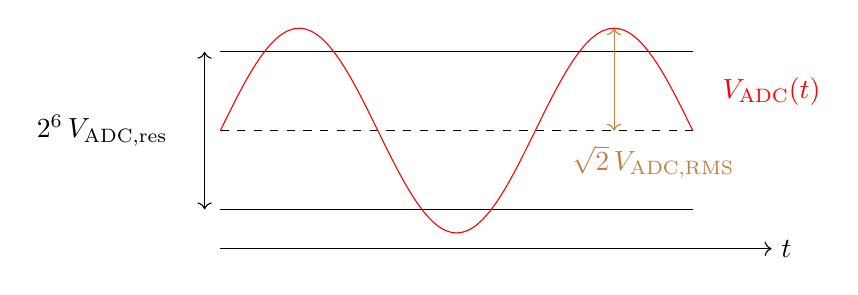
\begin{tikzpicture}[scale=1]
% Axes:
\draw [->] (-3,0) -- (4,0) node [right]  {$t$};
\draw (-3,0.5) -- (3,0.5) ;
\draw[dashed] (-3,1.5) -- (3,1.5) ;
\draw (-3,2.5) -- (3,2.5) ;
\draw[red] (-3,1.5) sin (-2,2.8) cos (-1,1.5) sin (0,0.2) cos (1,1.5) sin (2,2.8) cos (3,1.5);
\draw[<->] (-3.2,0.5) -- (-3.2,2.5);
\node (Vres) [] at (-4.5,1.5) {$2^6 \, V_{\te{ADC,res}}$};
\draw[<->,brown] (2,1.5) -- (2,2.8);
\node (Vadc) [brown] at (2.5,1.1) {$\sqrt{2} \, V_\te{ADC,RMS}$};
\node (Vadc) [red] at (4,2) {$V_\te{ADC}(t)$};
\end{tikzpicture}
\caption{Resolution and RMS values of ADC voltage}
\label{fig:ADC_res}
\end{figure}

Then, one can compute the transimpedance gain, which maps the RMS values of the input current to the output voltage:
\[
 R_2 = \frac{V_\te{ADC,RMS}}{I_{\te{mic,min,RMS}}} = \SI{3.81}{M\ohm}.
\]
The maximum microphone RMS current appears when the ADC voltage is maximum:
\[
 I_{\te{mic,max,RMS}} = \frac{V_\te{CC}/(2\sqrt{2})}{R_2} = \SI{232}{nA},
\]
corresponding to a maximal input sound pressure of
\[
   p_\te{max} = \frac{I_{\te{mic,max,RMS}}}{S_{\te{I,mic}}} = \SI{8.1}{mPa} \quad \Rightarrow \quad L_{p,\te{max}} = 20\log_{10}\left(\frac{p_\te{max}}{p_0}\right) = \SI{52.1}{dB_{SPL}}.
\]
The input spreads from \SI{16}{dB_{SPL}} to \SI{52.1}{dB_{SPL}}, giving a variation of \SI{36.1}{dB}. It is worth noting that, when expressed in dB, the input variation is exactly equal to the 6-bit output variation\footnote{This is the difference between the bit resolution of the ADC (12) and the number of bits used for the minimum detectable signal (6).} since 
\[
 20\log_{10}\left(2^{6}\right) = \SI{36.1}{dB}.
\]
Thereby, there is a trade-off between the number of bits dedicated to the minimum ADC signal (6 bits) and the input pressure range (6 bits) since they sum to the ADC resolution (12 bits). Still, the maximum input sound pressure of \SI{52.1}{dB_{SPL}} suits quite well the requirements of this work, for which a louder sound is rarely produced by birds (about \SI{60}{dB_{SPL}} at the source~\cite{10.1007/s00265-009-0743-4}).

Figure~\ref{fig:mic_scales} depicts the three main variables of the sensing subsystem expressed in dB scale: the input sound pressure $p$, the microphone voltage $V_{\te{mic}}$ and the output voltage $V_\te{ADC}$.
The output ADC voltage has been fixed by the microcontroller specifications.
The minimum input sound pressure, expressed both in \si{dB} and \si{dB_{SPL}}, has then been mapped to the minimum ADC voltage. In turn, it fixed the maximum input sound pressure since the input pressure range has the same length as the output voltage range previously set.

The only remaining degree of freedom for the microphone and amplification circuit lies in the relative position of the scale in between, characterizing the microphone voltage $V_\te{mic}$. This voltage is obtained from the input sound through the microphone sensitivity $S_{\te{mic,dB}}$, and is converted to the ADC voltage through the voltage gain of the amplification circuit:
\[
 G_{V,\te{dB}} = \frac{V_\te{ADC,RMS}}{V_\te{mic,RMS}} = \frac{R_2 \, I_\te{mic,RMS}}{V_\te{mic,RMS}} = \frac{R_2}{R_\te{L}} \quad \si{[dB]}.
\]
Since the input/output relation is given by
\begin{align*}
  p_\te{dB} + S_{\te{mic,dB}} + G_{\te{V,dB}} &= V_\te{ADC,RMS} \quad \si{[dB]},\\
  \SI{16}{dB} - \SI{94}{dB} + S_{\te{mic,dB}} + G_{\te{V,dB}} &= 
  \SI{-37.2}{dB},
\end{align*}
the scale of the microphone voltage needs to be adapted according to
\[
 S_{\te{mic,dB}} + G_{\te{V,dB}} = \SI{40.8}{dB}.
\]
This relation is useful for a parallel optimization of both the microphone and amplification circuit aiming at selecting the best noise/current consumption characteristic. However, the previous microphone selection has fixed the sensitivity at \SI{-24}{dB} and directly leads to a voltage gain of \SI{64.8}{dB}.

Finally, the figure highlights that the self-noise for this microphone (\SI{14}{dB_{SPL}}) is below the minimum input sound pressure. Brought back to the input pressure domain, the AFE noise will also be computed and added to this intrinsic microphone noise.

\begin{figure}[H]
\centering
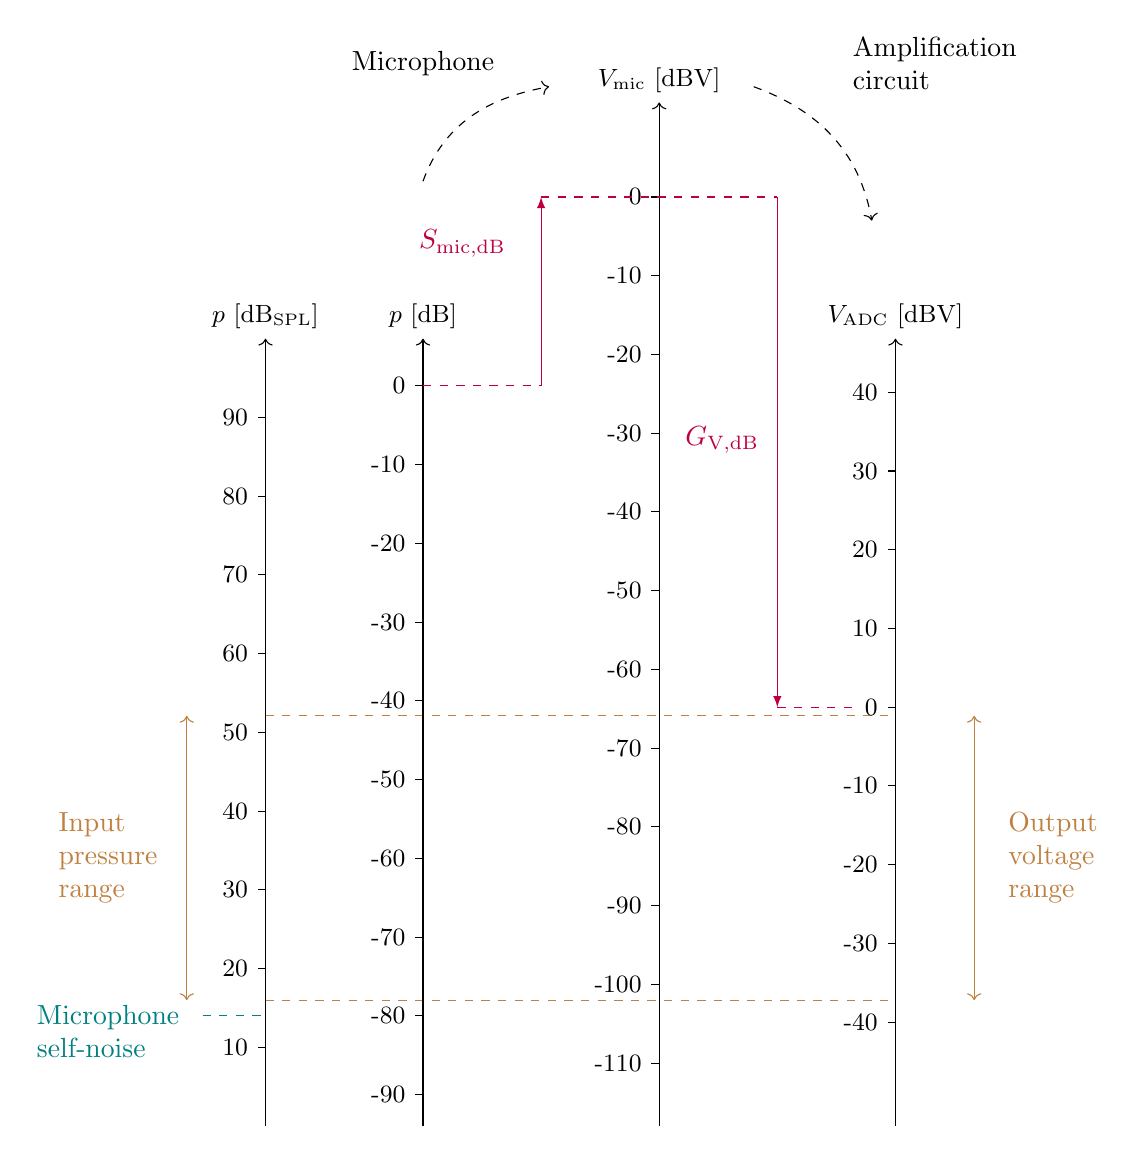
\begin{tikzpicture}[scale=1]
\def\SPLmin{1.6}
\def\res{3.61}
\def\vmin{3.72}
\def\Sens{2.4}
\draw[dashed, brown] (-4,\SPLmin) -- (4,\SPLmin) ;
\draw[dashed, brown] (-4,\SPLmin+\res) -- (4,\SPLmin+\res) ;
\draw[<->,brown] (-5,\SPLmin) -- (-5,\SPLmin+\res);
\node (Vadc) [brown,align=left] at (-6,\SPLmin+\res/2) {Input\\pressure\\range};
\draw[<->,brown] (5,\SPLmin) -- (5,\SPLmin+\res);
\node (Vadc) [brown,align=left] at (6,\SPLmin+\res/2) {Output\\voltage\\range};
\draw[->](-4,0)--(-4,10)node[font=\small,above]{$p$ [\si{dB_{SPL}}]};
\foreach\y in {10,20,...,90}{
 \draw[](-4,\y/10)--(-4.1,\y/10)node[left,font=\small]{$\y$};
}
\draw[->](-2,0)--(-2,10)node[font=\small,above]{$p$ [\si{dB}]};
\foreach\y in {-90,-80,...,0}{
 \draw[](-2,\y/10+9.4)--(-2.1,\y/10+9.4)node[left,font=\small]{\y};
}
\draw[->](1,0)--(1,13)node[font=\small,above]{$V_\te{mic}$ [\si{dBV}]};
\foreach\y in {-110,-100,...,0}{
 \draw[](1,\y/10+9.4+\Sens)--(0.9,\y/10+9.4+\Sens)node[left,font=\small]{\y};
}
\draw[->](4,0)--(4,10)node[font=\small,above]{$V_\te{ADC}$ [\si{dBV}]};
\foreach\y in {-40,-30,...,40}{
 \draw[](4,\y/10+\SPLmin+\vmin)--(3.9,\y/10+\SPLmin+\vmin)node[left,font=\small]{\y};
}
\draw[dashed, purple] (-2,9.4) -- (-0.5,9.4) ;
\draw[dashed, purple] (-0.5,9.4+\Sens) -- (2.5,9.4+\Sens) ;
\draw[latex-, purple](-0.5,9.4+\Sens)--(-0.5,9.4);
\draw[latex-, purple](2.5,\SPLmin+\vmin)--(2.5,9.4+\Sens);
\draw[dashed, purple] (2.5,\SPLmin+\vmin) -- (3.5,\SPLmin+\vmin) ;
\node (Vadc) [purple,align=left] at (1.8,\SPLmin+\res+3.5) {$G_{\te{V,dB}}$};
\node (Vadc) [purple,align=left] at (-1.5,\SPLmin+\res+6) {$S_{\te{mic,dB}}$};
\draw[->,dashed] (-2,12.0) to [out=70,in=190] (-0.4,13.2) ;
\draw[->,dashed] (2.2,13.2) to [out=-20,in=100] (3.7,11.5) ;
\node (Vadc) [] at (-2,13.5) {Microphone};
\node (Vadc) [align=left] at (4.5,13.5) {Amplification\\circuit};
\node (Vadc) [teal,align=left] at (-6,1.2) {Microphone\\self-noise};
\draw[dashed, teal] (-4.8,1.4) -- (-4,1.4) ;
\end{tikzpicture}
\caption{Range of $p$, $V_{\te{mic}}$ and $V_\te{ADC}$ along the dB scale}
\label{fig:mic_scales}
\end{figure}

\iffalse
\[
 V_\te{N,mic,ADC} = 10^{-\te{SNR}/20} \, S_{\te{mic}} \, G_{\te{V}} = \SI{205}{\micro V}
\]
is not much detected since it is less than the ADC resolution.
This microphone output noise voltage is then compared to the ADC voltage resolution, expressed as peak values:
\[
 \te{Microphone Noise Ratio} = \frac{\sqrt{2} \, V_\te{N,mic,ADC}}{V_{\te{ADC,res}}/2} = \SI{79}{\%}.
\]
\fi

The feedback capacitor $C_2$ compensates for parasitic capacitance at the op-amp inverting input which can cause instability. It also forms a high frequency pole with resistor $R_2$ in the response of the amplifier. According to the frequency range specified for the input sound pressure, the frequency of this pole must be $f_\te{H} = \SI{20}{kHz}$. The feedback capacitor value can then be calculated as
\[
 C_2 = \frac{1}{2 \pi \, f_\te{H} \, R_2} = \SI{2.09}{pF}.
\]

\subsubsection*{Microphone bias resistor and coupling capacitor}

The internal JFET of the electret microphone being biased by resistor $R_1$, the value of this resistor can be calculated from the desired supply voltage ($V_\te{CC}$), the microphone operating voltage ($V_\te{mic}$) and the current consumption ($I_\te{mic}$):
\[
 R_1 = \frac{V_\te{CC} - V_\te{mic}}{I_\te{mic}} = \SI{2.38}{k\ohm}.
\]
Resistor $R_1$ and capacitor $C_1$ form a high-pass filter, the corner frequency of this filter must be low enough not to attenuate low-frequency sound waves. As specified in the input frequency range, a corner frequency of $f_\te{L} = \SI{20}{Hz}$ is used to calculate the value of $C_1$:
\[
 C_1 = \frac{1}{2 \pi \, f_\te{L} \, R_1} = \SI{3.34}{\micro F}.
\]
One can see that reducing $R_1$ (for a higher and thus better microphone operating voltage) requires a larger capacitance (implying more space and cost).

\subsubsection*{Operational amplifier}

The required slew rate of the amplifier can be determined by calculating the maximum rate of change at the op-amp output, arising  for a sine wave at $f_\te{max} = \SI{20}{kHz}$ and an amplitude of $V_\te{CC}/2$ which sweeps the full output range. For sine waves, it can be shown\footnote{This is the highest slope of a sine function, appearing when the signal crosses 0.} that the slew rate is computed as
\[
 \te{SR} = 2 \pi f_\te{max} \frac{V_\te{CC}}{2} = \SI{0.188}{V/\micro s}.
\]
As a conservative rule, it is advised to select ten times this slew rate to eliminate any possibility of slew-induced distortion, which is very important in the analysis of audio data. This sets the required slew rate to \SI{1.88}{V/\micro s}.

The op-amp is selected such that it adds negligible noise to the output of the amplification circuit, avoiding the degradation of the data processing. However, such low-noise operational amplifiers consume a lot of power. One thus has to analyze and compare several state-of-the-art op-amps in order to choose the one which suits the best this noise/power consumption trade-off for this application.

The related op-amp parameters that need to be well selected are the current consumption (quiescent current $I_\te{Q}$), the input current noise spectral density $I_\te{N}$ and the input voltage noise spectral density $E_\te{NV}$.

The ADC voltage noise at the output is based on three noise contributions. The first noise is the thermal noise from resistors $R_1$ and $R_2$:
\[
 E_\te{NR} = \sqrt{4 \, k_\te{B} \, T \, (R_1 \parallelsum R_2)} = \SI{6.26}{nV/\sqrt{Hz}}
\]
where $T = \SI{300}{K}$ is the temperature and $k_\te{B} = \SI{1.38e-23}{J/K}$ is the Boltzmann constant.

The second noise contribution is the op-amp input current noise:
\[
 E_\te{NI} = I_\te{N} \, (R_1 \parallelsum R_2) \quad \left[\si{V/\sqrt{Hz}}\right].
\]
The last noise supply is due to the op-amp input voltage noise $E_\te{NV}$.

The output noise spectral density, for non-correlated contributions, of the amplifier circuit is then given by
\[
 E_\te{N,ADC} = A_\te{N} \sqrt{E_\te{NR}^2 + E_\te{NI}^2 + E_\te{NV}^2} \quad \left[\si{V/\sqrt{Hz}}\right]
\]
for which
\[
 A_\te{N} = 1 + \frac{R_2}{R_1} = 1602
\]
is the noise gain of the op-amp (see Appendix~\ref{appendix:noise_gain} for details). Since the signal gain is directly determined by $R_2$, it cannot be changed. On the other hand, a very low supply voltage $V_\te{CC}$ decreases the value of $R_1$, which increases the noise gain of the op-amp. Hence, the noise/power consumption trade-off also appears in the design of $R_1$.

Finally, the RMS output noise voltage can be computed by multiplying the output noise spectral density by the square of the bandwidth of integration (spreading over an A-weighting curve). An A-weighting curve can be approximated using a \SI{13.5}{kHz} noise bandwidth $B_\te{A}$, the RMS output noise voltage is thus (in RMS value)
\[
 V_\te{N,ADC} = \sqrt{B_\te{A}} \, E_\te{N,ADC} \quad [\si{V}].
\]
This noise contribution is then brought back to the input pressure domain, the \textit{input-referred noise} from the AFE is thus given by
\begin{align*}
  p_\te{IRN,AFE} &= \frac{V_\te{N,ADC}}{R_2\,S_{\te{I,mic}}}\\
   &= \frac{\sqrt{B_\te{A}}}{R_2\,S_{\te{I,mic}}} \left(1 + \frac{R_2}{R_1}\right) \sqrt{4 \, k_\te{B} \, T \, (R_1 \parallelsum R_2) + I_\te{N}^2 \, (R_1 \parallelsum R_2)^2 + E_\te{NV}^2} \quad \si{[Pa]}.
\end{align*}
One can directly see that this noise is roughly independent from the gain $R_2$ since $(1+R_2/R_1)/R_2\simeq 1/R_1$ in our design and the contribution from $I_\te{N}$ is typically negligible compared to $E_\te{NV}^2$.

\iffalse
As for the microphone noise, this output noise voltage is compared to the ADC voltage resolution, expressed as peak values:
\[
 \te{Op Amp Noise Ratio} = \frac{\sqrt{2} \, V_\te{N,ADC}}{V_{\te{ADC,res}}/2} \quad [\%].
\]
\fi

Since the total input-referred noise is composed of non-correlated sources (from the microphone $p_{\te{SN}}$ and the AFE $ p_\te{IRN,AFE}$), their noise powers add up to give
\[
 p_\te{IRN} = \sqrt{p_{\te{SN}}^2 + p_\te{IRN,AFE}^2} \quad \si{[Pa]}.
\]

Figure~\ref{fig:output_noise_op_amp} presents this input-referred noise with respect to the current consumption for several operational amplifiers. Clearly, the input-referred noise must not exceed the minimum signal sound pressure of \SI{16}{dB_{SPL}}.

The ultra-low-power LMV551 op-amp has a quiescent current of only \SI{37}{\micro A}, but the input-referred noise of \SI{17.85}{dB_{SPL}} exceeds the minimum detectable input pressure.
In order to keep the noise voltage not much detected from the ADC, the input-referred noise typically needs to be smaller than the minimum input signal (as depicted in Figure~\ref{fig:ADC_res_noise}).

The OPA2834 has an input-referred noise of $p_\te{IRN,OA} = \SI{14.22}{dB_{SPL}}$ while keeping a particularly small current consumption of \SI{170}{\micro A}. One finally selects this op-amp since it has the lowest noise in the group of three op-amps which belong to an acceptable range of quiescent current (from \SI{100}{\micro A} to \SI{200}{\micro A}).

\begin{figure}[H]
    \centering
    % This file was created by matlab2tikz.
%
%The latest updates can be retrieved from
%  http://www.mathworks.com/matlabcentral/fileexchange/22022-matlab2tikz-matlab2tikz
%where you can also make suggestions and rate matlab2tikz.
%
\definecolor{mycolor1}{rgb}{0.00000,0.44700,0.74100}%
\definecolor{mycolor2}{rgb}{0.85000,0.32500,0.09800}%
\definecolor{mycolor3}{rgb}{0.92900,0.69400,0.12500}%
\definecolor{mycolor4}{rgb}{0.49400,0.18400,0.55600}%
\definecolor{mycolor5}{rgb}{0.46600,0.67400,0.18800}%
\definecolor{mycolor6}{rgb}{0.00000,1.00000,1.00000}%
%
\begin{tikzpicture}

\begin{axis}[%
width=4.521in,
height=3.566in,
at={(0.758in,0.481in)},
scale only axis,
xmode=log,
xmin=10,
xmax=10000,
xminorticks=true,
xlabel style={font=\color{white!15!black}},
xlabel={Quiescent current [\si{\micro A}]},
ymin=14,
ymax=18,
ylabel style={font=\color{white!15!black}},
ylabel={Input-referred noise [\si{dB_{SPL}}]},
axis background/.style={fill=white},
xmajorgrids,
xminorgrids,
ymajorgrids,
legend style={legend cell align=left, align=left, draw=none}
]
\addplot [color=mycolor1, dashed, line width=2.0pt]
  table[row sep=crcr]{%
10	16\\
10000	16\\
};
\addlegendentry{Min. signal}

\addplot [color=mycolor2, draw=none, mark size=4.2pt, mark=*, mark options={solid, mycolor2}]
  table[row sep=crcr]{%
1001	14.0528160320545\\
};
\addlegendentry{OPA838}

\addplot [color=mycolor3, draw=none, mark size=4.2pt, mark=*, mark options={solid, mycolor3}]
  table[row sep=crcr]{%
650	14.0706044064729\\
};
\addlegendentry{OPA1692}

\addplot [color=mycolor4, draw=none, mark size=4.2pt, mark=*, mark options={solid, mycolor4}]
  table[row sep=crcr]{%
385	14.1437057977188\\
};
\addlegendentry{OPA2188}

\addplot [color=mycolor5, draw=none, mark size=4.2pt, mark=*, mark options={solid, mycolor5}]
  table[row sep=crcr]{%
170	14.2236495465669\\
};
\addlegendentry{OPA2834}

\addplot [color=mycolor6, draw=none, mark size=4.2pt, mark=*, mark options={solid, mycolor6}]
  table[row sep=crcr]{%
130	14.2850975057981\\
};
\addlegendentry{OPA314}

\addplot [color=black, draw=none, mark size=4.2pt, mark=*, mark options={solid, black}]
  table[row sep=crcr]{%
110	14.3928725960103\\
};
\addlegendentry{LMV651}

\addplot [color=blue, draw=none, mark size=4.2pt, mark=*, mark options={solid, blue}]
  table[row sep=crcr]{%
60	15.0413180279693\\
};
\addlegendentry{TLV9001}

\addplot [color=green, draw=none, mark size=4.2pt, mark=*, mark options={solid, green}]
  table[row sep=crcr]{%
37	17.8471165996574\\
};
\addlegendentry{LMV551}

\end{axis}
\end{tikzpicture}%

    \caption{Comparison of input-referred noise and current consumption for several operational amplifiers}
    \label{fig:output_noise_op_amp}
\end{figure}

\begin{figure}[H]
\centering
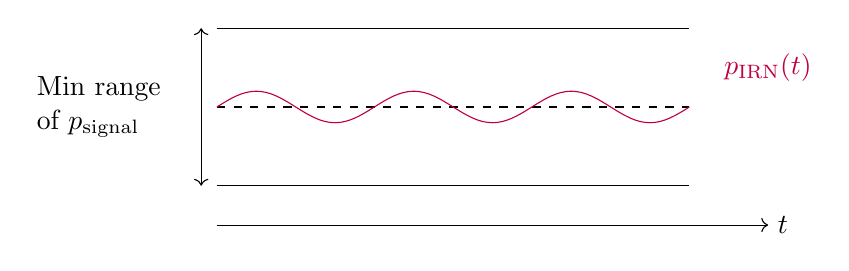
\begin{tikzpicture}[scale=1]
% Axes:
\draw [->] (-3,0) -- (4,0) node [right]  {$t$};
\draw (-3,0.5) -- (3,0.5) ;
\draw[dashed] (-3,1.5) -- (3,1.5) ;
\draw (-3,2.5) -- (3,2.5) ;
\draw[purple] (-3,1.5) sin (-2.5,1.7) cos (-2,1.5) sin (-1.5,1.3) cos (-1,1.5) sin (-0.5,1.7) cos (0,1.5) sin (0.5,1.3) cos (1,1.5) sin (1.5,1.7) cos (2,1.5) sin (2.5,1.3) cos (3,1.5);
\draw[<->] (-3.2,0.5) -- (-3.2,2.5);
\node (Vres) [align=left] at (-4.5,1.5) {Min range\\of $p_{\te{signal}}$};
\node (Vadc) [purple] at (4,2) {$p_\te{IRN}(t)$};
\end{tikzpicture}
\caption{Voltage noise and resolution at the amplification output}
\label{fig:ADC_res_noise}
\end{figure}

%Summing the noise contributions from the microphone and the operational amplifier leads to a total output voltage of 90\% compared to the ADC resolution. One thus expects a maximum digitized error of 1 consecutive code level introduced by the ADC quantization.

In the end, the OPA2834 op-amp characteristics are given in Table~\ref{tab:selected_op_amp}. The slew rate of \SI{26}{V/\micro s} is well above the limit of \SI{1.88}{V/\micro s}.

\begin{table}[H]
\centering
\scalebox{0.95}{
\begin{tabular}{lccc}
\toprule
 Criteria            & Required    & OPA2834    & Units             \\ \midrule
 Supply voltage      & 2.5         & 2.5 -- 5.4 & V                 \\
 Quiescent current   & < 200       & 170        & \si{\micro A}     \\
 Input voltage noise & < 27        & 12         & \si{nV/\sqrt{Hz}} \\
 Input current noise & N/A         & 0.2        & \si{pA/\sqrt{Hz}} \\
 Slew rate           & > 1.88      & 26         & \si{V/\micro s}   \\
 \bottomrule
\end{tabular}
}
\caption{Characteristics of the selected operational amplifier: OPA2834}
\label{tab:selected_op_amp}
\end{table}


\subsubsection*{AFE noise voltage}

The noise voltage from the AFE can be theoretically computed over an A-weighting curve of bandwidth $B_\te{A} = \SI{13.5}{kHz}$ as
\[
 V_\te{N,ADC,theor} = \sqrt{B_\te{A}} \, E_\te{N,ADC} = \SI{2.52}{mV}
\]
where $E_\te{N,ADC}$ depends on the voltage and current noise of the OPA2834.

As a validation of the amp op selection, Figure~\ref{fig:output_noise_op_amp_freq} describes the noise voltage spectral density at the amplification output. 
This noise is the combination of flicker (or $1/f$) noise and thermal (flat band) noise. Hence, it depends on the frequency and is higher for frequencies below the $1/f$ corner frequency: \SI{150}{Hz} for the voltage noise and \SI{900}{Hz} for the current noise, as given in the op-amp datasheet. Since audio signals contain frequencies that are particularly low, the noise is sadly impinged by flicker noise. For a frequency of \SI{22}{Hz}, the noise reaches \SI{37}{\micro V/\sqrt{Hz}}.

Since the noise contribution from the microphone is not represented in the simulation, this simulated noise can be compared to the theoretical value of the AFE noise (\SI{2.52}{mV}). Due to the frequency dependence, one needs to integrate the noise power spectral density over the whole frequency range in order to obtain the output noise voltage:
\[
 V_\te{N,ADC,simu} = \sqrt{\int_{0}^{\infty} E_\te{N,ADC}(f)^2 \, \te{d}f} = \SI{2.37}{mV}.
\]
As expected, the result is very similar to the theoretical one, hence not impinging the previous conclusions for the choice of the best operational amplifier.

%This small contribution compared to the microphone noise makes the total voltage noise in the order of the ADC resolution (104\%), which still allows a low-noise digitization.

\begin{figure}[H]
    \centering
    % This file was created by matlab2tikz.
%
%The latest updates can be retrieved from
%  http://www.mathworks.com/matlabcentral/fileexchange/22022-matlab2tikz-matlab2tikz
%where you can also make suggestions and rate matlab2tikz.
%
\definecolor{mycolor1}{rgb}{0.00000,0.44700,0.74100}%
%
\begin{tikzpicture}

\begin{axis}[%
width=4.521in,
height=3.566in,
at={(0.758in,0.481in)},
scale only axis,
xmode=log,
xmin=10,
xmax=100000,
xminorticks=true,
xlabel style={font=\color{white!15!black}},
xlabel={Frequency [Hz]},
ymode=log,
ymin=1,
ymax=100,
yminorticks=true,
ylabel style={font=\color{white!15!black}},
ylabel={Noise spectral density [\si{\micro V/\sqrt{Hz}}]},
axis background/.style={fill=white},
xmajorgrids,
xminorgrids,
ymajorgrids,
yminorgrids
]
\addplot [color=mycolor1, line width=2.0pt, forget plot]
  table[row sep=crcr]{%
10	32.99847\\
10.2329299228075	33.19928\\
10.471285480509	33.39667\\
10.7151930523761	33.59047\\
10.9647819614319	33.7805\\
11.2201845430196	33.9666\\
11.4815362149688	34.14858\\
11.7489755493953	34.32625\\
12.0226443461741	34.49944\\
12.3026877081238	34.66797\\
12.5892541179417	34.83164\\
12.8824955169313	34.99028\\
13.1825673855641	35.1437\\
13.4896288259165	35.29173\\
13.8038426460288	35.4342\\
14.1253754462275	35.57092\\
14.4543977074593	35.70173\\
14.7910838816821	35.82648\\
15.1356124843621	35.945\\
15.4881661891248	36.05715\\
15.8489319246111	36.16278\\
16.2181009735893	36.26177\\
16.5958690743756	36.35399\\
16.9824365246174	36.43933\\
17.3780082874937	36.51769\\
17.7827941003892	36.58898\\
18.1970085860998	36.65311\\
18.6208713666287	36.71004\\
19.0546071796325	36.75969\\
19.4984459975804	36.80204\\
19.9526231496888	36.83706\\
20.4173794466953	36.86473\\
20.8929613085404	36.88506\\
21.3796208950223	36.89806\\
21.8776162394955	36.90377\\
22.3872113856834	36.90222\\
22.9086765276777	36.89349\\
23.4422881531992	36.87762\\
23.9883291901949	36.85472\\
24.5470891568503	36.82488\\
25.1188643150958	36.7882\\
25.7039578276886	36.74481\\
26.3026799189538	36.69485\\
26.9153480392691	36.63844\\
27.5422870333816	36.57576\\
28.1838293126445	36.50695\\
28.840315031266	36.4322\\
29.5120922666638	36.35167\\
30.1995172040201	36.26556\\
30.9029543251359	36.17405\\
31.6227766016838	36.07735\\
32.3593656929628	35.97565\\
33.1131121482591	35.86916\\
33.8844156139202	35.75809\\
34.6736850452531	35.64265\\
35.4813389233575	35.52305\\
36.3078054770101	35.39951\\
37.1535229097172	35.27224\\
38.0189396320561	35.14146\\
38.904514499428	35.00737\\
39.8107170553497	34.87019\\
40.7380277804112	34.73013\\
41.6869383470335	34.58739\\
42.6579518801592	34.44218\\
43.6515832240165	34.2947\\
44.6683592150963	34.14515\\
45.7088189614874	33.9937\\
46.7735141287197	33.84057\\
47.8630092322638	33.68592\\
48.9778819368445	33.52993\\
50.1187233627272	33.37278\\
51.2861383991364	33.21464\\
52.4807460249772	33.05566\\
53.7031796370252	32.896\\
54.9540873857623	32.73582\\
56.2341325190348	32.57527\\
57.5439937337156	32.41446\\
58.8843655355588	32.25355\\
60.2559586074357	32.09266\\
61.6595001861481	31.93192\\
63.0957344480192	31.77143\\
64.5654229034654	31.6113\\
66.0693448007595	31.45166\\
67.608297539198	31.29259\\
69.1830970918935	31.13419\\
70.7945784384136	30.97656\\
72.4435960074988	30.81976\\
74.1310241300916	30.66389\\
75.8577575029182	30.50903\\
77.624711662869	30.35522\\
79.4328234724279	30.20256\\
81.2830516164097	30.05109\\
83.1763771102669	29.90088\\
85.1138038202374	29.75198\\
87.0963589956078	29.60443\\
89.1250938133743	29.45828\\
91.2010839355907	29.31358\\
93.3254300796988	29.17036\\
95.4992586021433	29.02865\\
97.7237220955808	28.88849\\
99.9999999999997	28.74991\\
102.329299228075	28.61294\\
104.71285480509	28.47758\\
107.15193052376	28.34388\\
109.647819614318	28.21183\\
112.201845430196	28.08147\\
114.815362149688	27.95279\\
117.489755493953	27.82582\\
120.226443461741	27.70055\\
123.026877081238	27.57701\\
125.892541179416	27.45518\\
128.824955169313	27.33508\\
131.82567385564	27.2167\\
134.896288259165	27.10004\\
138.038426460288	26.98511\\
141.253754462275	26.8719\\
144.543977074592	26.7604\\
147.91083881682	26.65062\\
151.35612484362	26.54253\\
154.881661891248	26.43613\\
158.489319246111	26.33142\\
162.181009735893	26.22839\\
165.958690743756	26.12701\\
169.824365246174	26.02729\\
173.780082874937	25.9292\\
177.827941003892	25.83274\\
181.970085860998	25.73789\\
186.208713666286	25.64463\\
190.546071796324	25.55296\\
194.984459975804	25.46284\\
199.526231496887	25.37428\\
204.173794466952	25.28724\\
208.929613085403	25.20172\\
213.796208950222	25.1177\\
218.776162394954	25.03515\\
223.872113856833	24.95405\\
229.086765276777	24.8744\\
234.422881531991	24.79617\\
239.883291901948	24.71935\\
245.470891568502	24.6439\\
251.188643150957	24.56982\\
257.039578276885	24.49709\\
263.026799189537	24.42567\\
269.15348039269	24.35556\\
275.422870333816	24.28673\\
281.838293126444	24.21917\\
288.403150312659	24.15285\\
295.120922666637	24.08775\\
301.9951720402	24.02386\\
309.029543251358	23.96115\\
316.227766016837	23.89959\\
323.593656929627	23.83919\\
331.13112148259	23.7799\\
338.844156139201	23.72171\\
346.73685045253	23.6646\\
354.813389233574	23.60856\\
363.0780547701	23.55355\\
371.535229097171	23.49956\\
380.18939632056	23.44658\\
389.045144994279	23.39457\\
398.107170553495	23.34352\\
407.380277804111	23.29341\\
416.869383470333	23.24421\\
426.579518801591	23.19592\\
436.515832240164	23.1485\\
446.683592150961	23.10195\\
457.088189614873	23.05623\\
467.735141287196	23.01133\\
478.630092322636	22.96723\\
489.778819368444	22.9239\\
501.18723362727	22.88134\\
512.861383991362	22.83952\\
524.80746024977	22.79842\\
537.03179637025	22.75801\\
549.540873857622	22.71829\\
562.341325190346	22.67923\\
575.439937337154	22.64081\\
588.843655355586	22.60301\\
602.559586074355	22.5658\\
616.595001861479	22.52918\\
630.95734448019	22.49312\\
645.654229034652	22.4576\\
660.693448007592	22.4226\\
676.082975391978	22.38811\\
691.830970918933	22.35409\\
707.945784384134	22.32052\\
724.435960074986	22.2874\\
741.310241300914	22.2547\\
758.57757502918	22.22239\\
776.247116628688	22.19045\\
794.328234724277	22.15887\\
812.830516164095	22.12763\\
831.763771102666	22.09669\\
851.138038202372	22.06604\\
870.963589956076	22.03565\\
891.250938133741	22.00551\\
912.010839355905	21.97559\\
933.254300796986	21.94586\\
954.992586021431	21.9163\\
977.237220955805	21.8869\\
999.999999999994	21.85761\\
1023.29299228075	21.82843\\
1047.12854805089	21.79931\\
1071.5193052376	21.77024\\
1096.47819614318	21.7412\\
1122.01845430196	21.71214\\
1148.15362149688	21.68305\\
1174.89755493952	21.65389\\
1202.26443461741	21.62464\\
1230.26877081237	21.59527\\
1258.92541179416	21.56575\\
1288.24955169313	21.53604\\
1318.2567385564	21.50612\\
1348.96288259164	21.47595\\
1380.38426460288	21.44549\\
1412.53754462274	21.41472\\
1445.43977074592	21.3836\\
1479.1083881682	21.35209\\
1513.5612484362	21.32015\\
1548.81661891247	21.28776\\
1584.8931924611	21.25486\\
1621.81009735892	21.22142\\
1659.58690743755	21.1874\\
1698.24365246173	21.15276\\
1737.80082874936	21.11745\\
1778.27941003891	21.08142\\
1819.70085860997	21.04465\\
1862.08713666286	21.00706\\
1905.46071796324	20.96863\\
1949.84459975803	20.9293\\
1995.26231496887	20.88903\\
2041.73794466952	20.84775\\
2089.29613085402	20.80543\\
2137.96208950222	20.762\\
2187.76162394954	20.71741\\
2238.72113856832	20.67161\\
2290.86765276776	20.62455\\
2344.22881531991	20.57615\\
2398.83291901947	20.52638\\
2454.70891568501	20.47516\\
2511.88643150956	20.42244\\
2570.39578276885	20.36815\\
2630.26799189536	20.31225\\
2691.5348039269	20.25465\\
2754.22870333815	20.19531\\
2818.38293126443	20.13416\\
2884.03150312658	20.07113\\
2951.20922666636	20.00616\\
3019.95172040199	19.9392\\
3090.29543251357	19.87017\\
3162.27766016836	19.79901\\
3235.93656929626	19.72566\\
3311.31121482589	19.65006\\
3388.441561392	19.57215\\
3467.36850452529	19.49187\\
3548.13389233573	19.40915\\
3630.78054770099	19.32395\\
3715.3522909717	19.23621\\
3801.89396320558	19.14586\\
3890.45144994278	19.05287\\
3981.07170553494	18.95719\\
4073.80277804109	18.85876\\
4168.69383470332	18.75755\\
4265.79518801589	18.65351\\
4365.15832240162	18.54662\\
4466.8359215096	18.43683\\
4570.88189614871	18.32412\\
4677.35141287194	18.20848\\
4786.30092322634	18.08987\\
4897.78819368442	17.96829\\
5011.87233627268	17.84372\\
5128.61383991361	17.71618\\
5248.07460249768	17.58565\\
5370.31796370248	17.45215\\
5495.4087385762	17.3157\\
5623.41325190344	17.17631\\
5754.39937337152	17.03401\\
5888.43655355584	16.88885\\
6025.59586074353	16.74085\\
6165.95001861477	16.59006\\
6309.57344480188	16.43655\\
6456.5422903465	16.28036\\
6606.9344800759	16.12158\\
6760.82975391976	15.96026\\
6918.30970918931	15.7965\\
7079.45784384132	15.63037\\
7244.35960074984	15.46197\\
7413.10241300911	15.29139\\
7585.77575029177	15.11874\\
7762.47116628685	14.94413\\
7943.28234724275	14.76766\\
8128.30516164092	14.58945\\
8317.63771102664	14.40963\\
8511.38038202369	14.22832\\
8709.63589956073	14.04564\\
8912.50938133738	13.86173\\
9120.10839355902	13.67671\\
9332.54300796983	13.49072\\
9549.92586021428	13.30389\\
9772.37220955802	13.11637\\
9999.99999999991	12.92828\\
10232.9299228075	12.73976\\
10471.2854805089	12.55095\\
10715.193052376	12.36198\\
10964.7819614318	12.17298\\
11220.1845430195	11.9841\\
11481.5362149687	11.79544\\
11748.9755493952	11.60715\\
12022.644346174	11.41934\\
12302.6877081237	11.23214\\
12589.2541179416	11.04566\\
12882.4955169312	10.86002\\
13182.567385564	10.67532\\
13489.6288259164	10.49167\\
13803.8426460287	10.30918\\
14125.3754462274	10.12793\\
14454.3977074591	9.948032\\
14791.0838816819	9.769558\\
15135.6124843619	9.592597\\
15488.1661891247	9.417226\\
15848.931924611	9.24352\\
16218.1009735891	9.071547\\
16595.8690743754	8.90137\\
16982.4365246173	8.73305\\
17378.0082874936	8.566641\\
17782.7941003891	8.402192\\
18197.0085860997	8.239752\\
18620.8713666285	8.07936\\
19054.6071796323	7.921054\\
19498.4459975803	7.764866\\
19952.6231496886	7.610828\\
20417.3794466951	7.458962\\
20892.9613085402	7.309291\\
21379.6208950221	7.161832\\
21877.6162394953	7.016601\\
22387.2113856832	6.873609\\
22908.6765276775	6.732863\\
23442.288153199	6.594369\\
23988.3291901947	6.458129\\
24547.0891568501	6.324142\\
25118.8643150956	6.192407\\
25703.9578276884	6.062917\\
26302.6799189536	5.935666\\
26915.3480392689	5.810643\\
27542.2870333814	5.687837\\
28183.8293126443	5.567235\\
28840.3150312658	5.448822\\
29512.0922666636	5.332581\\
30199.5172040199	5.218495\\
30902.9543251356	5.106543\\
31622.7766016835	4.996705\\
32359.3656929625	4.888961\\
33113.1121482588	4.783285\\
33884.4156139199	4.679657\\
34673.6850452528	4.57805\\
35481.3389233572	4.478441\\
36307.8054770098	4.380801\\
37153.5229097169	4.285107\\
38018.9396320557	4.191331\\
38904.5144994277	4.099445\\
39810.7170553493	4.009422\\
40738.0277804108	3.921234\\
41686.9383470331	3.834852\\
42657.9518801588	3.750249\\
43651.5832240161	3.667396\\
44668.3592150958	3.586264\\
45708.818961487	3.506824\\
46773.5141287193	3.429049\\
47863.0092322633	3.35291\\
48977.8819368441	3.278376\\
50118.7233627267	3.205422\\
51286.1383991359	3.134018\\
52480.7460249767	3.064136\\
53703.1796370247	2.995748\\
54954.0873857619	2.928826\\
56234.1325190343	2.863344\\
57543.9937337151	2.799273\\
58884.3655355583	2.736587\\
60255.9586074351	2.675259\\
61659.5001861475	2.615262\\
63095.7344480186	2.556571\\
64565.4229034648	2.49916\\
66069.3448007589	2.443004\\
67608.2975391974	2.388077\\
69183.0970918929	2.334354\\
70794.578438413	2.281811\\
72443.5960074982	2.230425\\
74131.0241300909	2.180171\\
75857.7575029175	2.131026\\
77624.7116628683	2.082967\\
79432.8234724272	2.035972\\
81283.051616409	1.990019\\
83176.3771102661	1.945085\\
85113.8038202367	1.901149\\
87096.3589956071	1.858191\\
89125.0938133735	1.816189\\
91201.0839355899	1.775123\\
93325.430079698	1.734973\\
95499.2586021425	1.69572\\
97723.7220955799	1.657343\\
100000	1.619826\\
};
\end{axis}
\end{tikzpicture}%

    \caption{Noise voltage spectral density from AFE at the amplification output (from \textsc{LTspice})}
    \label{fig:output_noise_op_amp_freq}
\end{figure}

\subsubsection*{Total noise voltage}

One can then compute the total noise voltage $V_\te{N,tot,theor}$ at the amplification output, resulting from the microphone noise and the AFE noise:
\[
 V_\te{N,tot,theor} = p_\te{IRN} \, R_2\,S_{\te{I,mic}} = \SI{11.2}{mV}.
\]


\subsubsection*{Op amp bias network}

Resistors $R_3$ and $R_4$ center the op-amp input and output at the midpoint between the power supplies to allow the widest possible output signal swing. Therefore $R_3 = R_4$ for $V_\te{B} = V_\te{CC} / 2$. The value of these resistors needs to be very high in order to limit the power supply current drawn by this voltage divider. However, the non-zero op-amp input bias current prevents the bias voltage $V_\te{B}$ to be exactly at $V_\te{CC} / 2$, and this variation worsens with the resistance of the bias resistors. A reasonable choice consists to set a maximum bias voltage relative variation of 0.5\%:
\[
 \Delta V_\te{B} = \frac{1}{2} \, R_3 \, I_\te{b+} < 0.005 V_\te{B} \quad \Rightarrow \quad R_3 < 0.01 \frac{V_\te{CC}}{2I_\te{b+}} = \SI{179}{k\ohm}
\]
where $I_\te{b+} = \SI{70}{nA}$ for the selected op-amp. A final value of
\[
 R_3 = R_4 = \SI{150}{k\ohm}
\]
is finally chosen, which implies a current in the voltage divider of approximately
\[
 I_\te{B} = \frac{V_\te{CC}}{R_3 + R_4} = \SI{8.33}{\micro A}.
\]
This current is small (less than 5\%) compared to the microphone bias current, and is a good trade-off between the power consumption and the bias voltage stability.

Capacitor $C_3$ is included to filter thermal noise created by the resistors and any noise which may be present on the power supply. The corner frequency of the low-pass filter is formed by $R_3$, $R_4$ and $C_3$. It should be well below the operating frequency range in order to prevent noise from affecting the audio performance of the design. A corner frequency of $f_\te{B} = \SI{5}{Hz}$ is selected:
\[
 C_3 = \frac{1}{2 \pi \, f_\te{B} \, (R_3 \parallelsum R_4)} = \SI{424}{nF}.
\]

\subsubsection*{Summary}

Table~\ref{tab:selected_values_microphone} summarizes the theoretical values for the amplification circuit as well as the values actually put on the experimental device depending on the available components.

\begin{table}[H]
\centering
\begin{tabular}{lcc}
\toprule
             & \multicolumn{2}{c}{Value}                \\
             & Theoretical         & Real               \\ \midrule
 $R_1$       & \SI{2.38}{k\ohm}    & \SI{2.37}{k\ohm}   \\
 $R_2$       & \SI{3.81}{M\ohm}    & \SI{3.83}{M\ohm}   \\
 $R_3$       & \SI{150}{k\ohm}     & \SI{150}{k\ohm}    \\
 $R_4$       & \SI{150}{k\ohm}     & \SI{150}{k\ohm}    \\
 $C_1$       & \SI{3.34}{\micro F} & \SI{3.3}{\micro F} \\
 $C_2$       & \SI{2.09}{pF}       & \SI{2}{pF}         \\
 $C_3$       & \SI{424}{nF}        & \SI{470}{nF}       \\ \bottomrule
\end{tabular}
\caption{Final values for the amplification circuit}
\label{tab:selected_values_microphone}
\end{table}

Figure~\ref{fig:microphone_AC} presents the AC transfer function of the amplification circuit from the input pressure to the output voltage, which confirms a bandwidth ranging from \SI{20}{Hz} to \SI{20}{kHz}. The important phase variations (with additional poles) are due to the intrinsic behavior of the electret microphone.

\begin{figure}[H]
    \centering
    % This file was created by matlab2tikz.
%
%The latest updates can be retrieved from
%  http://www.mathworks.com/matlabcentral/fileexchange/22022-matlab2tikz-matlab2tikz
%where you can also make suggestions and rate matlab2tikz.
%
\definecolor{mycolor1}{rgb}{0.00000,0.44700,0.74100}%
\definecolor{mycolor2}{rgb}{0.85000,0.32500,0.09800}%
%
\begin{tikzpicture}

\begin{axis}[%
width=4.476in,
height=3.566in,
at={(0.758in,0.481in)},
scale only axis,
xmode=log,
xmin=1,
xmax=100000,
xminorticks=true,
xlabel style={font=\color{white!15!black}},
xlabel={Frequency [Hz]},
separate axis lines,
every outer y axis line/.append style={mycolor2},
every y tick label/.append style={font=\color{mycolor2}},
every y tick/.append style={mycolor2},
ymin=-300,
ymax=200,
ylabel style={font=\color{mycolor2}},
ylabel={Phase [deg]},
axis background/.style={fill=white},
yticklabel pos=right,
xmajorgrids,
xminorgrids,
ymajorgrids
]
\addplot [color=mycolor1, line width=2.0pt, forget plot]
  table[row sep=crcr]{%
1	-22.409818016676\\
1.25892541179417	-18.4179303175973\\
1.58489319246111	-14.4307617566398\\
1.99526231496888	-10.4510353737672\\
2.51188643150958	-6.48301154856172\\
3.16227766016838	-2.53330705327609\\
3.98107170553497	1.38791914103049\\
5.01187233627272	5.26534575672286\\
6.30957344480194	9.07649273455381\\
7.94328234724282	12.7897232368718\\
10	16.3631807793871\\
12.5892541179417	19.7461858384809\\
15.8489319246111	22.884433008991\\
19.9526231496888	25.7283707300627\\
25.1188643150958	28.2411118638283\\
31.6227766016838	30.4017388768831\\
39.8107170553498	32.2041443377122\\
50.1187233627273	33.6558600908952\\
63.0957344480194	34.7794315235055\\
79.4328234724283	35.6132838021949\\
100	36.2078422519237\\
125.892541179417	36.6173429334429\\
158.489319246112	36.8916495134126\\
199.526231496888	37.0714539412103\\
251.188643150958	37.1871851153386\\
316.227766016838	37.2601902269273\\
398.107170553498	37.3047006717061\\
501.187233627273	37.3297007796822\\
630.957344480194	37.3403500791733\\
794.328234724283	37.3388944228404\\
1000	37.3251048362941\\
1258.92541179417	37.2963015092179\\
1584.89319246112	37.2470262113192\\
1995.26231496888	37.1684816176994\\
2511.88643150959	37.0480358985201\\
3162.27766016839	36.8694750563515\\
3981.07170553498	36.6152241459442\\
5011.87233627273	36.2718280297549\\
6309.57344480195	35.8373486317116\\
7943.28234724283	35.3173941552237\\
10000	34.6534462109619\\
12589.2541179417	33.4174746003498\\
15848.9319246112	30.4259873902836\\
19952.6231496889	25.179998026209\\
25118.8643150959	18.9117589328704\\
31622.7766016839	12.5095980186292\\
39810.7170553498	6.19490698038523\\
50118.7233627274	-0.0201451335304876\\
63095.7344480195	-6.16067308065276\\
79432.8234724284	-12.2508786767516\\
100000	-18.308320478059\\
};
\addplot [color=mycolor2, dashed, line width=2.0pt, forget plot]
  table[row sep=crcr]{%
1	175.839887033033\\
1.25892541179417	174.764984999263\\
1.58489319246111	173.413951956995\\
1.99526231496888	171.717452580955\\
2.51188643150958	169.590297064096\\
3.16227766016838	166.929317500623\\
3.98107170553497	163.612452919725\\
5.01187233627272	159.500695230795\\
6.30957344480194	154.445578787028\\
7.94328234724282	148.305715600782\\
10	140.9750275386\\
12.5892541179417	132.420328423658\\
15.8489319246111	122.715831001165\\
19.9526231496888	112.053777369463\\
25.1188643150958	100.718772775273\\
31.6227766016838	89.0412388100291\\
39.8107170553498	77.3626037736009\\
50.1187233627273	66.0229028679115\\
63.0957344480194	55.3467036664255\\
79.4328234724283	45.6057544382253\\
100	36.9728043592778\\
125.892541179417	29.4990949561464\\
158.489319246112	23.1278019661448\\
199.526231496888	17.7290034584652\\
251.188643150958	13.1356945238758\\
316.227766016838	9.16955456285955\\
398.107170553498	5.65484752740218\\
501.187233627273	2.42328952328281\\
630.957344480194	-0.686697196241501\\
794.328234724283	-3.83377068027825\\
1000	-7.17884484985917\\
1258.92541179417	-10.8905583945186\\
1584.89319246112	-15.1500880214791\\
1995.26231496888	-20.154221698959\\
2511.88643150959	-26.1155965931627\\
3162.27766016839	-33.260319265583\\
3981.07170553498	-41.8287572445617\\
5011.87233627273	-52.1005687439252\\
6309.57344480195	-64.4966968360495\\
7943.28234724283	-79.8594313738753\\
10000	-100.00591155895\\
12589.2541179417	-127.849345249403\\
15848.9319246112	-162.620546917467\\
19952.6231496889	-193.754125559825\\
25118.8643150959	-215.140320126683\\
31622.7766016839	-229.245654695143\\
39810.7170553498	-238.999091916536\\
50118.7233627274	-246.083382042128\\
63095.7344480195	-251.415746921222\\
79432.8234724284	-255.529762496834\\
100000	-258.762170176612\\
};
\end{axis}
\end{tikzpicture}%
    \caption{AC transfer function of the amplification circuit (from \textsc{LTspice})}
    \label{fig:microphone_AC}
\end{figure}

As stated before, the classical trade-off between noise and power consumption was not worth considering in the microphone selection since the other microphones suffer from too high noise. However, if the constraint on the minimum detectable sound wave were relaxed, the choice of the microphone and operational amplifier would have to be optimized conjointly by computing the input-referred noise and power consumption of the whole sensing subsystem.


\chapter{Data processing and transceiver}

Data are processed in a microcontroller and received/transmitted in a transceiver. For this work, a CMWX1ZZABZ chip from Murata is used, which combines an STM32L072 microcontroller and an SX1276 transceiver. Its operation voltage range is \SI{2.2}{V} -- \SI{3.6}{V}.

\section{Microcontroller}

The STM32L072 is an ultra-low-power microcontroller incorporating an Arm Cortex-M0+ 32-bit RISC core operating at a 32 MHz frequency, with embedded memories (192 Kbytes of Flash program memory, 6 Kbytes of data EEPROM and 20 Kbytes of RAM), a 12-bit ADC with hardware oversampling,\dots ~It operates from a \SI{1.8}{V} to \SI{3.6}{V} power supply~\cite{STM32L072xx}.

\subsection*{ADC characteristics}

A 12-bit analog-to-digital converter (ADC) has been used to digitize (sampling and quantization) two signals: the analog microphone voltage and supercap voltage. The resolution of an $N$-bit ADC is given by $V_\te{DD}/2^N$ where $V_\te{DD}$ is the supply voltage. One might be interested to improve the ADC resolution up to 14 bits via diverse techniques (such as SAR, etc). This would allow the reading of a smaller input sound pressure (\SI{12}{dB} below) and make possible to process a sound pressure of \SI{4}{dB_{SPL}} (increasing the detectable distance between the sensor and the source). However, the signal quality would not benefit from this increased ADC resolution because the microphone self-noise is still \SI{14}{dB_{SPL}}.

A typical code alternates between an energy-intensive run mode (to sample sound) and a low-power sleep mode. The duty cycle between these modes will be determined in the section characterizing the power consumption (Section~\ref{section:power_consumption}).

\subsection*{Status of supercapacitor charge}

In order to know the status of the supercapacitor charge and adapt the MCU code to a possible overdischarge, the ADC reads the supercap voltage. Since this voltage is higher than the ADC supply voltage, a voltage divider is required. The supercap voltage is thus divided by two with two resistors $R_\te{SC}$ of same resistance, which has to be determined according to the impedance recommendations at the ADC input. Provided in the datasheet, the maximum input impedance for an error below 1/4 of LSB is given by (derived from the charge equation of the internal sample-and-hold capacitor)
\[
 R_\te{AIN,max} = \frac{T_\te{S}}{f_\te{ADC}\,C_\te{ADC}\,\ln(2^{N+2})} - R_\te{ADC} = \SI{257}{k\ohm}
\]
where $T_\te{S} = 160.5$ is the number of cycles per sample, $f_\te{ADC} = \SI{8}{MHz}$ is the ADC clock frequency, $C_\te{ADC} = \SI{8}{pF}$ is the internal sample-and-hold capacitor, $N=12$ is the number of resolution bits and $R_\te{ADC} = \SI{1}{k\ohm}$ is the sampling switch resistance. To increase $R_\te{AIN,max}$ and thus reduce power consumption, parameters such as $T_\te{S}$ and $f_\te{ADC}$ are pushed towards a low sampling frequency $f_\te{s} = f_\te{ADC}/T_\te{S}$ equal to \SI{49.8}{kHz} in this case (the delay between each sampling being not important since the supercapacitor undergoes low variations).

Because $R_\te{AIN,max}$ corresponds to $R_\te{SC}/2$, one selects a resistance $R_\te{SC}$ of \SI{475}{k\ohm}. This value produces a negligible current consumption of
\[
 I_\te{SC,ADC} = \frac{V_\te{SC}}{2R_\te{SC}} = \SI{4.7}{\micro A}
\]
in the worst-case scenario when the supercapacitor is fully charged at \SI{4.5}{V}.

Finally, the ADC input leakage current provided in the datasheet is maximum $I_\te{in,ADC} = \SI{50}{nA}$. The ADC voltage due to the non-zero input current is thus $(V_\te{SC} - R_\te{SC}\,I_\te{in,ADC})/2$ instead of $V_\te{SC}/2$, leading to a maximum relative error of
\[
 E_\te{rel} = \frac{R_\te{SC}\,I_\te{in,ADC}}{V_\te{SC}} = \SI{0.85}{\%}
\]
in the worst-case scenario when the supercapacitor is fully discharged (\SI{2.8}{V}). This error is negligible.


\section{Transceiver}

The SX1276 transceiver features a LoRa long-range modem that provides ultra-long range spread spectrum communication~\cite{SX1276}. LoRa has been increasingly used in the IoT domain thanks to their compromise between range, interference immunity and energy consumption~\cite{SINHA201714}. The transceiver chip is connected to an external ISM (industrial, scientific and medical purposes) antenna in the range \SI{790}{MHz} -- \SI{960}{MHz}.

The receiver is used for over-the-air (OTA) updates and thus implies that the MCU has reconfiguration capabilities to keep up with application, security and communication protocol updates. During such updates, the challenge is the instantaneous power consumption when the wireless radio is in receive mode and the microcontroller is reprogramming its internal Flash memory (recall that the maximum current consumption at the PMU output is \SI{80}{mA} and that the energy storage is very limited). To lower this peak power, a smart decomposition of the firmware packets is required.

The transmitter is used to send data to a gateway, mainly information about the analyzed input sound pressure and hence bird species. All data are handled in the RAM memory of the MCU, but important data that need to be transmitted are stored in the FLASH memory in order to prevent them from being erased after an unexpected shutdown.

The radio-frequency communication for this smart sensor, including power consumption and security in LoRaWAN networks, has been carefully discussed and optimized in a concurrent master thesis~\cite{Hess2020}.


\chapter{Power supply}

In this chapter, the total current consumption is evaluated. The solar cells and supercapacitor are then sized accordingly.

\section{Power consumption}
\label{section:power_consumption}

The power consumption will be computed separately for each block. Since the voltage regulator inside the PMU is an LDO, the current drawn in the circuit is the same as the current drawn in the supercapacitor. For each subsystem, it thus makes sense to provide the current consumption $I$ instead of the power consumption since the latter is higher from the supercap point of view ($V_\te{SC}\,I$) than from the subsystem point of view ($V_\te{DD}\,I$).


\subsection*{Sensing}

As seen in Figure~\ref{fig:circuit_AFE}, the current consumption from the sensing subsystem is composed of
\begin{itemize}
 \item the current through the microphone branch (with $R_1$): $I_{\te{mic}} = \SI{358}{\micro A}$ (see Table~\ref{tab:op_point_mic}),
 \item the op-amp quiescent current: $I_\te{Q} = \SI{170}{\micro A}$,
 \item and the current through the voltage divider with $R_3$ and $R_4$ to bias the op-amp: $I_\te{B} = \SI{8.33}{\micro A}$.
\end{itemize}

This leads to a current consumption of $I_\te{sensing} = \SI{536}{\micro A}$.

\subsection*{Power Management}

The current consumption of the power management subsystem is composed of
\begin{itemize}
 \item the leakage current of the supercapacitor: typically $I_\te{Q,SC} = \SI{500}{\micro A}$ (will be refined in Section~\ref{supercap_sizing}),
 \item the voltage divider to read the supercap voltage at the ADC input $I_\te{SC,ADC} = \SI{4.7}{\micro A}$,
 \item and the PMU quiescent current: $I_\te{Q,PMU} = \SI{0.6}{\micro A}$.
\end{itemize}

This leads to a current consumption of $I_\te{power} = \SI{505}{\micro A}$.


\subsection*{Data processing and transceiver}

%The power supply $VDD_{STM32}$ required for the STM32 being between \SI{1.8}{V} and \SI{3.6}{V}, one has to choose a trade-off between a small power consumption (small voltage) and a high signal resolution from the microphone (high voltage). A voltage of $VDD_{STM32} = \SI{3}{V}$ has finally been selected.

For this part, it is possible to adapt the code in the microcontroller to match the best capabilities of the system.
In view of the power consumption from the previous parts and the typical harvested power from solar cells, one will aim to keep the MCU/RF consumption below \SI{4}{mA}. 

\subsubsection*{First case without transceiver}

As a first approximation, a run mode that only processes data is considered (that is, without transmission or reception). A typical scheme for this application is to alternate a run mode and standby mode.

Addressing a simple scheme allows using a simulation tool (Wisebatt) in order to estimate the power consumption. As seen in Figure~\ref{fig:wisebatt1}, Wisebatt estimates the run mode at \SI{2.74}{mA} and the standby mode at \SI{3.64}{\micro A}. With a duty cycle of $1/3$, one obtains an average current consumption of
\[
 i_\te{avg} = \frac{1}{3} \, \SI{2.74}{mA} + \frac{2}{3} \, \SI{3.64}{\micro A} = \SI{0.913}{mA}.
\]

By assuming that it takes \SI{50}{ms} to sample and process the data, it leads to a cycle duration of \SI{150}{ms}. However, the simulation tool misses the FFT operation that is achieved inside the microcontroller, which significantly reduces the current consumption in run mode. To refine this poor model, experimental measurements of the current consumption have been achieved (see Figure~\ref{fig:consumption_fft}). With a duty cycle of $1/3$, they show an average current consumption of \SI{3.88}{mA} since the run mode consumes \SI{10.1}{mA}. An MCU current consumption of \SI{3.88}{mA} will be kept as reference for designing further components, it allows keeping a precise track of the input sound wave (one third of the time at high run/sleep cycle frequency) with sufficiently low power consumption. It is worth noting that the increase in current consumption before each sleep mode is due to the microcontroller which saves the data by writing in its registers (and write operations consume more than the read operations appearing at the beginning of each run mode).

\begin{figure}[H]
\begin{subfigure}{.49\textwidth}
  \centering
    % This file was created by matlab2tikz.
%
%The latest updates can be retrieved from
%  http://www.mathworks.com/matlabcentral/fileexchange/22022-matlab2tikz-matlab2tikz
%where you can also make suggestions and rate matlab2tikz.
%
\definecolor{mycolor1}{rgb}{0.00000,0.44700,0.74100}%
%
\begin{tikzpicture}[scale=0.6]

\begin{axis}[%
width=4.521in,
height=3.566in,
at={(0.758in,0.481in)},
scale only axis,
xmin=0,
xmax=2.5,
xlabel style={font=\color{white!15!black}},
xlabel={Time [s]},
ymin=0,
ymax=3,
ylabel style={font=\color{white!15!black}},
ylabel={Current [mA]},
axis background/.style={fill=white},
xmajorgrids,
ymajorgrids
]
\addplot [color=mycolor1, line width=2.0pt, forget plot]
  table[row sep=crcr]{%
0	0\\
0.099999	0\\
0.1	2.742253856\\
0.149999	2.742253856\\
0.15	0.003548066103\\
0.249999	0.003548066103\\
0.25	2.742279451\\
0.299999	2.742279451\\
0.3	0.003573661302\\
0.399999	0.003573661302\\
0.4	2.742304643\\
0.449999	2.742304643\\
0.45	0.003598853417\\
0.549999	0.003598853417\\
0.55	2.742329443\\
0.599999	2.742329443\\
0.6	0.003623652797\\
0.699999	0.003623652797\\
0.7	2.742353859\\
0.749999	2.742353859\\
0.75	0.003648069454\\
0.849999	0.003648069454\\
0.85	2.742377903\\
0.899999	2.742377903\\
0.9	0.003672113064\\
0.999999	0.003672113064\\
1	2.742401583\\
1.049999	2.742401583\\
1.05	0.00369579297\\
1.149999	0.00369579297\\
1.15	2.742424909\\
1.199999	2.742424909\\
1.2	0.003719118175\\
1.299999	0.003719118175\\
1.3	2.742447888\\
1.349999	2.742447888\\
1.35	0.003742097352\\
1.449999	0.003742097352\\
1.45	2.742470529\\
1.499999	2.742470529\\
1.5	0.003764738835\\
1.599999	0.003764738835\\
1.6	2.742492841\\
1.649999	2.742492841\\
1.65	0.003787050622\\
1.749999	0.003787050622\\
1.75	2.742514831\\
1.799999	2.742514831\\
1.8	0.003809040376\\
1.899999	0.003809040376\\
1.9	2.742536506\\
1.949999	2.742536506\\
1.95	0.003830715424\\
2.049999	0.003830715424\\
2.05	2.742557874\\
2.099999	2.742557874\\
2.1	0.003852082758\\
2.199999	0.003852082758\\
2.2	2.74257894\\
2.249999	2.74257894\\
2.25	0.003873149033\\
2.349999	0.003873149033\\
2.35	2.742599712\\
2.399999	2.742599712\\
2.4	0.003893920567\\
2.499999	0.003893920567\\
};
\end{axis}
\end{tikzpicture}%

    \caption{Wisebatt simulation}
    \label{fig:wisebatt1}
\end{subfigure}
\begin{subfigure}{.49\textwidth}
  \centering
  % This file was created by matlab2tikz.
%
%The latest updates can be retrieved from
%  http://www.mathworks.com/matlabcentral/fileexchange/22022-matlab2tikz-matlab2tikz
%where you can also make suggestions and rate matlab2tikz.
%
\definecolor{mycolor1}{rgb}{0.00000,0.44700,0.74100}%
%
\begin{tikzpicture}[scale=0.6]

\begin{axis}[%
width=4.521in,
height=3.566in,
at={(0.758in,0.481in)},
scale only axis,
xmin=0,
xmax=300,
xlabel style={font=\color{white!15!black}},
xlabel={Time [ms]},
ymin=0,
ymax=12,
ylabel style={font=\color{white!15!black}},
ylabel={Current [mA]},
axis background/.style={fill=white},
xmajorgrids,
ymajorgrids
]
\addplot [color=mycolor1, line width=2.0pt, forget plot]
  table[row sep=crcr]{%
0	8.1685203158\\
0.100002000000002	9.0823187391\\
0.200003000000001	9.1015091163\\
0.300004	9.1106948904\\
0.400006000000001	9.101985526\\
0.500007	9.5448380961\\
0.600009000000002	10.114058333\\
0.700010000000001	9.9120606299\\
0.799991999999999	10.119015971\\
0.899993000000002	10.061191747\\
0.999994000000001	10.099393847\\
1.099996	10.076153988\\
1.199997	10.102788266\\
1.299999	10.077151471\\
1.4	10.100197789\\
1.500002	10.083181031\\
1.600003	10.071508994\\
1.700004	10.068724975\\
1.800006	10.073697501\\
1.900007	10.047792724\\
2.000009	10.081066963\\
2.10001	10.096118531\\
2.200012	10.094793517\\
2.300013	10.080664992\\
2.399994	10.097309555\\
2.499996	10.068099687\\
2.599997	10.092530571\\
2.699999	10.056874284\\
2.8	10.081439158\\
2.900002	10.050219436\\
3.000003	10.080694768\\
3.100004	10.084372055\\
3.200006	10.106495329\\
3.300007	10.091801068\\
3.400009	10.095523019\\
3.50001	10.075067178\\
3.600012	10.089463683\\
3.700013	10.076079549\\
3.800015	10.070213755\\
3.900016	10.068576097\\
4.000017	10.060104937\\
4.099999	10.102773379\\
4.2	10.082466416\\
4.300002	10.106361339\\
4.400003	10.065717638\\
4.500005	10.067146867\\
4.600006	10.078163841\\
4.700007	10.054402909\\
4.800009	10.045693544\\
4.90001	10.060700449\\
5.000012	10.043103067\\
5.100013	10.086158591\\
5.200015	10.071434555\\
5.300016	10.060923766\\
5.400017	10.096654492\\
5.500019	10.061489503\\
5.60002	10.088585303\\
5.700002	10.053911611\\
5.800003	10.053063006\\
5.900005	10.056189445\\
6.000006	10.029331849\\
6.100007	10.088704405\\
6.200009	10.083970084\\
6.30001	10.087751586\\
6.400012	10.077791646\\
6.500013	10.06652158\\
6.600015	10.078521149\\
6.700016	10.063916214\\
6.800017	10.068442106\\
6.900019	10.058824586\\
7.00002	10.037386151\\
7.100022	10.071077247\\
7.200023	10.341648168\\
7.300025	10.399383066\\
7.400006	10.373016768\\
7.500007	10.415759648\\
7.600009	10.425555822\\
7.70001	10.417397307\\
7.800012	10.56364019\\
7.900013	10.526465347\\
8.000015	10.545893929\\
8.100016	10.570295037\\
8.200018	10.664683704\\
8.300019	10.868319066\\
8.40002	10.902695001\\
8.500022	11.267952345\\
8.600023	11.088405448\\
8.700025	10.891290945\\
8.800026	10.533224409\\
8.900028	10.560037341\\
9.000029	10.627449311\\
9.10001	10.971387322\\
9.200012	11.001430907\\
9.300013	11.102027788\\
9.400015	11.5519074\\
9.500016	10.76118644\\
9.600018	10.218109184\\
9.700019	10.221176071\\
9.80002	9.8748560118\\
9.900022	9.8693773005\\
10.000023	9.9177626583\\
10.100025	10.166910031\\
10.200026	8.9399615725\\
10.300028	4.2296246605\\
10.400029	0.37340097188\\
10.50003	0.35083106345\\
10.600032	0.35485077009\\
10.700033	0.34649871295\\
10.800015	0.34964003925\\
10.900016	0.32705524302\\
11.000018	0.32948195481\\
11.100019	0.33497555389\\
11.20002	0.3312536033\\
11.300022	0.37466643508\\
11.400023	0.35982329609\\
11.500025	0.35418081898\\
11.600026	0.35005689772\\
11.700028	0.35602690648\\
11.800029	0.34398267434\\
11.90003	0.3275614283\\
12.000032	0.34897008815\\
12.100033	0.3262959651\\
12.200035	0.32596843344\\
12.300036	0.36685033882\\
12.400018	0.35498476031\\
12.500019	0.36591240727\\
12.600021	0.34727287867\\
12.700022	0.34447397182\\
12.800023	0.34690068361\\
12.900025	0.34197282102\\
13.000026	0.33515420752\\
13.100028	0.34428043039\\
13.200029	0.32144254152\\
13.300031	0.334365154\\
13.400032	0.3735200743\\
13.500033	0.36384300274\\
13.600035	0.34675180559\\
13.700036	0.35360019469\\
13.800038	0.3381019924\\
13.900039	0.35102460488\\
14.000021	0.31728884465\\
14.100022	0.35224540467\\
14.200023	0.32474763365\\
14.300025	0.3368960804\\
14.400026	0.36888996775\\
14.500028	0.35876626212\\
14.600029	0.35211141445\\
14.700031	0.35279625336\\
14.800032	0.35047375619\\
14.900033	0.33767024613\\
15.000035	0.33592837325\\
15.100036	0.34134753332\\
15.200038	0.32841003304\\
15.300039	0.33339744684\\
15.400041	0.36135673974\\
15.500042	0.36302417361\\
15.600043	0.35651820396\\
15.700025	0.35584825285\\
15.800026	0.33609213907\\
15.900028	0.34359559148\\
16.000029	0.32601309685\\
16.100031	0.34026072374\\
16.200032	0.33135781791\\
16.300034	0.32251446329\\
16.400035	0.35144146334\\
16.500036	0.36076122764\\
16.600038	0.35145635115\\
16.700039	0.35625022352\\
16.800041	0.34639449833\\
16.900042	0.34203237223\\
17.000044	0.33229574946\\
17.100045	0.33701518282\\
17.200046	0.33433537839\\
17.300048	0.32774008193\\
17.400029	0.3455756692\\
17.500031	0.3536746337\\
17.600032	0.36685033882\\
17.700034	0.34414644017\\
17.800035	0.34874677111\\
17.900036	0.35543139439\\
18.000038	0.32063860019\\
18.100039	0.34304474279\\
18.200041	0.3318937788\\
18.300042	0.32715945764\\
18.400044	0.32921397437\\
18.500045	0.36820512884\\
18.600046	0.35474655548\\
18.700048	0.35395750195\\
18.800049	0.34261299652\\
18.900051	0.35170944379\\
19.000052	0.33781912415\\
19.100034	0.33549662698\\
19.200035	0.3244349898\\
19.300036	0.33865284109\\
19.400038	0.32803783798\\
19.500039	0.37152510877\\
19.600041	0.35010156113\\
19.700042	0.35952554004\\
19.800044	0.34907430276\\
19.900045	0.34289586477\\
20.000046	0.34045426518\\
20.100048	0.33954610923\\
20.200049	0.3343949296\\
20.300051	0.32648950653\\
20.400052	0.33077719362\\
20.500054	0.3536448581\\
20.600055	0.35447857503\\
20.700037	0.36804136301\\
20.800038	0.33944189461\\
20.900039	0.35650331616\\
21.000041	0.33457358323\\
21.100042	0.3399629677\\
21.200044	0.3300328035\\
21.300045	0.32720412104\\
21.400047	0.33433537839\\
21.500048	0.35750079892\\
21.600049	0.36077611545\\
21.700051	0.3623393347\\
21.800052	0.34134753332\\
21.900054	0.36040392039\\
22.000055	0.33147692033\\
22.100057	0.35293024358\\
22.200058	0.33056876439\\
22.300059	0.33059853999\\
22.400041	0.33607725127\\
22.500042	0.33525842214\\
22.600044	0.37116780152\\
22.700045	0.35354064348\\
22.800047	0.35732214529\\
22.900048	0.35645865275\\
23.000049	0.34106466507\\
23.100051	0.34103488947\\
23.200052	0.34018628473\\
23.300054	0.33213198364\\
23.400055	0.32681703818\\
23.500057	0.33472246125\\
23.600058	0.36702899245\\
23.700059	0.35462745306\\
23.800061	0.35163500477\\
23.900062	0.36007638873\\
24.000044	0.34846390286\\
24.100045	0.34445908402\\
24.200047	0.33461824664\\
24.300048	0.3250900531\\
24.400049	0.33123871549\\
24.500051	0.33704495843\\
24.600052	0.35343642886\\
24.700054	0.36363457351\\
24.800055	0.35699461364\\
24.900057	0.35124792191\\
25.000058	0.35263248753\\
25.10006	0.33859328988\\
25.200061	0.33844441185\\
25.300062	0.33525842214\\
25.400064	0.33013701812\\
25.500065	0.32647461873\\
25.600067	0.35455301404\\
25.700048	0.35931711081\\
25.80005	0.3449354937\\
25.900051	0.35997217412\\
26.000052	0.34697512262\\
26.100054	0.33927812879\\
26.200055	0.34006718231\\
26.300057	0.42686307028\\
26.400058	0.64440363888\\
26.50006	0.63761480099\\
26.600061	0.6606908947\\
26.700062	0.65422958846\\
26.800064	0.68276950565\\
26.900065	0.68675943669\\
27.000067	0.65784732444\\
27.100068	0.66276029923\\
27.20007	0.66545499146\\
27.300071	0.66475526475\\
27.400052	0.65342564713\\
27.500054	0.65129669139\\
27.600055	0.6693853713\\
27.700057	0.67054661988\\
27.800058	0.6706359467\\
27.90006	0.67668039447\\
28.000061	0.66337069913\\
28.100062	0.66031869964\\
28.200064	0.66977245416\\
28.300065	0.71704122676\\
28.400067	0.93754446804\\
28.500068	1.455669767\\
28.60007	1.4669100578\\
28.700071	1.7059337253\\
28.800073	1.8786471209\\
28.900074	1.8598438264\\
28.9000740000002	8.1685203158\\
29.0000760000002	9.0823187391\\
29.1000770000002	9.1015091163\\
29.2000780000002	9.1106948904\\
29.3000800000002	9.101985526\\
29.4000810000002	9.5448380961\\
29.5000830000002	10.114058333\\
29.6000840000002	9.9120606299\\
29.7000660000002	10.119015971\\
29.8000670000002	10.061191747\\
29.9000680000002	10.099393847\\
30.0000700000002	10.076153988\\
30.1000710000002	10.102788266\\
30.2000730000002	10.077151471\\
30.3000740000002	10.100197789\\
30.4000760000002	10.083181031\\
30.5000770000002	10.071508994\\
30.6000780000002	10.068724975\\
30.7000800000002	10.073697501\\
30.8000810000002	10.047792724\\
30.9000830000002	10.081066963\\
31.0000840000002	10.096118531\\
31.1000860000002	10.094793517\\
31.2000870000002	10.080664992\\
31.3000680000002	10.097309555\\
31.4000700000002	10.068099687\\
31.5000710000002	10.092530571\\
31.6000730000002	10.056874284\\
31.7000740000002	10.081439158\\
31.8000760000002	10.050219436\\
31.9000770000002	10.080694768\\
32.0000780000002	10.084372055\\
32.1000800000002	10.106495329\\
32.2000810000002	10.091801068\\
32.3000830000002	10.095523019\\
32.4000840000002	10.075067178\\
32.5000860000002	10.089463683\\
32.6000870000002	10.076079549\\
32.7000890000002	10.070213755\\
32.8000900000002	10.068576097\\
32.9000910000002	10.060104937\\
33.0000730000002	10.102773379\\
33.1000740000002	10.082466416\\
33.2000760000002	10.106361339\\
33.3000770000002	10.065717638\\
33.4000790000002	10.067146867\\
33.5000800000002	10.078163841\\
33.6000810000002	10.054402909\\
33.7000830000002	10.045693544\\
33.8000840000002	10.060700449\\
33.9000860000002	10.043103067\\
34.0000870000002	10.086158591\\
34.1000890000002	10.071434555\\
34.2000900000002	10.060923766\\
34.3000910000002	10.096654492\\
34.4000930000002	10.061489503\\
34.5000940000002	10.088585303\\
34.6000760000002	10.053911611\\
34.7000770000002	10.053063006\\
34.8000790000002	10.056189445\\
34.9000800000002	10.029331849\\
35.0000810000002	10.088704405\\
35.1000830000002	10.083970084\\
35.2000840000002	10.087751586\\
35.3000860000002	10.077791646\\
35.4000870000002	10.06652158\\
35.5000890000002	10.078521149\\
35.6000900000002	10.063916214\\
35.7000910000002	10.068442106\\
35.8000930000002	10.058824586\\
35.9000940000002	10.037386151\\
36.0000960000002	10.071077247\\
36.1000970000002	10.341648168\\
36.2000990000002	10.399383066\\
36.3000800000002	10.373016768\\
36.4000810000002	10.415759648\\
36.5000830000002	10.425555822\\
36.6000840000002	10.417397307\\
36.7000860000002	10.56364019\\
36.8000870000002	10.526465347\\
36.9000890000002	10.545893929\\
37.0000900000002	10.570295037\\
37.1000920000002	10.664683704\\
37.2000930000002	10.868319066\\
37.3000940000002	10.902695001\\
37.4000960000002	11.267952345\\
37.5000970000002	11.088405448\\
37.6000990000002	10.891290945\\
37.7001000000002	10.533224409\\
37.8001020000002	10.560037341\\
37.9001030000002	10.627449311\\
38.0000840000002	10.971387322\\
38.1000860000002	11.001430907\\
38.2000870000002	11.102027788\\
38.3000890000002	11.5519074\\
38.4000900000002	10.76118644\\
38.5000920000002	10.218109184\\
38.6000930000002	10.221176071\\
38.7000940000002	9.8748560118\\
38.8000960000002	9.8693773005\\
38.9000970000002	9.9177626583\\
39.0000990000002	10.166910031\\
39.1001000000002	8.9399615725\\
39.2001020000002	4.2296246605\\
39.3001030000002	0.37340097188\\
39.4001040000002	0.35083106345\\
39.5001060000002	0.35485077009\\
39.6001070000002	0.34649871295\\
39.7000890000002	0.34964003925\\
39.8000900000002	0.32705524302\\
39.9000920000002	0.32948195481\\
40.0000930000002	0.33497555389\\
40.1000940000002	0.3312536033\\
40.2000960000002	0.37466643508\\
40.3000970000002	0.35982329609\\
40.4000990000002	0.35418081898\\
40.5001000000002	0.35005689772\\
40.6001020000002	0.35602690648\\
40.7001030000002	0.34398267434\\
40.8001040000002	0.3275614283\\
40.9001060000002	0.34897008815\\
41.0001070000002	0.3262959651\\
41.1001090000002	0.32596843344\\
41.2001100000002	0.36685033882\\
41.3000920000002	0.35498476031\\
41.4000930000002	0.36591240727\\
41.5000950000002	0.34727287867\\
41.6000960000002	0.34447397182\\
41.7000970000002	0.34690068361\\
41.8000990000002	0.34197282102\\
41.9001000000002	0.33515420752\\
42.0001020000002	0.34428043039\\
42.1001030000002	0.32144254152\\
42.2001050000002	0.334365154\\
42.3001060000002	0.3735200743\\
42.4001070000002	0.36384300274\\
42.5001090000002	0.34675180559\\
42.6001100000002	0.35360019469\\
42.7001120000002	0.3381019924\\
42.8001130000002	0.35102460488\\
42.9000950000002	0.31728884465\\
43.0000960000002	0.35224540467\\
43.1000970000002	0.32474763365\\
43.2000990000002	0.3368960804\\
43.3001000000002	0.36888996775\\
43.4001020000002	0.35876626212\\
43.5001030000002	0.35211141445\\
43.6001050000002	0.35279625336\\
43.7001060000002	0.35047375619\\
43.8001070000002	0.33767024613\\
43.9001090000002	0.33592837325\\
44.0001100000002	0.34134753332\\
44.1001120000002	0.32841003304\\
44.2001130000002	0.33339744684\\
44.3001150000002	0.36135673974\\
44.4001160000002	0.36302417361\\
44.5001170000002	0.35651820396\\
44.6000990000002	0.35584825285\\
44.7001000000002	0.33609213907\\
44.8001020000002	0.34359559148\\
44.9001030000002	0.32601309685\\
45.0001050000002	0.34026072374\\
45.1001060000002	0.33135781791\\
45.2001080000002	0.32251446329\\
45.3001090000002	0.35144146334\\
45.4001100000002	0.36076122764\\
45.5001120000002	0.35145635115\\
45.6001130000002	0.35625022352\\
45.7001150000002	0.34639449833\\
45.8001160000002	0.34203237223\\
45.9001180000002	0.33229574946\\
46.0001190000002	0.33701518282\\
46.1001200000002	0.33433537839\\
46.2001220000002	0.32774008193\\
46.3001030000002	0.3455756692\\
46.4001050000002	0.3536746337\\
46.5001060000002	0.36685033882\\
46.6001080000002	0.34414644017\\
46.7001090000002	0.34874677111\\
46.8001100000002	0.35543139439\\
46.9001120000002	0.32063860019\\
47.0001130000002	0.34304474279\\
47.1001150000002	0.3318937788\\
47.2001160000002	0.32715945764\\
47.3001180000002	0.32921397437\\
47.4001190000002	0.36820512884\\
47.5001200000002	0.35474655548\\
47.6001220000002	0.35395750195\\
47.7001230000002	0.34261299652\\
47.8001250000002	0.35170944379\\
47.9001260000002	0.33781912415\\
48.0001080000002	0.33549662698\\
48.1001090000002	0.3244349898\\
48.2001100000002	0.33865284109\\
48.3001120000002	0.32803783798\\
48.4001130000002	0.37152510877\\
48.5001150000002	0.35010156113\\
48.6001160000002	0.35952554004\\
48.7001180000002	0.34907430276\\
48.8001190000002	0.34289586477\\
48.9001200000002	0.34045426518\\
49.0001220000002	0.33954610923\\
49.1001230000002	0.3343949296\\
49.2001250000002	0.32648950653\\
49.3001260000002	0.33077719362\\
49.4001280000002	0.3536448581\\
49.5001290000002	0.35447857503\\
49.6001110000002	0.36804136301\\
49.7001120000002	0.33944189461\\
49.8001130000002	0.35650331616\\
49.9001150000002	0.33457358323\\
50.0001160000002	0.3399629677\\
50.1001180000002	0.3300328035\\
50.2001190000002	0.32720412104\\
50.3001210000002	0.33433537839\\
50.4001220000002	0.35750079892\\
50.5001230000002	0.36077611545\\
50.6001250000002	0.3623393347\\
50.7001260000002	0.34134753332\\
50.8001280000002	0.36040392039\\
50.9001290000002	0.33147692033\\
51.0001310000002	0.35293024358\\
51.1001320000002	0.33056876439\\
51.2001330000002	0.33059853999\\
51.3001150000002	0.33607725127\\
51.4001160000002	0.33525842214\\
51.5001180000002	0.37116780152\\
51.6001190000002	0.35354064348\\
51.7001210000002	0.35732214529\\
51.8001220000002	0.35645865275\\
51.9001230000002	0.34106466507\\
52.0001250000002	0.34103488947\\
52.1001260000002	0.34018628473\\
52.2001280000002	0.33213198364\\
52.3001290000002	0.32681703818\\
52.4001310000002	0.33472246125\\
52.5001320000002	0.36702899245\\
52.6001330000002	0.35462745306\\
52.7001350000002	0.35163500477\\
52.8001360000002	0.36007638873\\
52.9001180000002	0.34846390286\\
53.0001190000002	0.34445908402\\
53.1001210000002	0.33461824664\\
53.2001220000002	0.3250900531\\
53.3001230000002	0.33123871549\\
53.4001250000002	0.33704495843\\
53.5001260000002	0.35343642886\\
53.6001280000002	0.36363457351\\
53.7001290000002	0.35699461364\\
53.8001310000002	0.35124792191\\
53.9001320000002	0.35263248753\\
54.0001340000002	0.33859328988\\
54.1001350000002	0.33844441185\\
54.2001360000002	0.33525842214\\
54.3001380000002	0.33013701812\\
54.4001390000002	0.32647461873\\
54.5001410000002	0.35455301404\\
54.6001220000002	0.35931711081\\
54.7001240000002	0.3449354937\\
54.8001250000002	0.35997217412\\
54.9001260000002	0.34697512262\\
55.0001280000002	0.33927812879\\
55.1001290000002	0.34006718231\\
55.2001310000002	0.42686307028\\
55.3001320000002	0.64440363888\\
55.4001340000002	0.63761480099\\
55.5001350000002	0.6606908947\\
55.6001360000002	0.65422958846\\
55.7001380000002	0.68276950565\\
55.8001390000002	0.68675943669\\
55.9001410000002	0.65784732444\\
56.0001420000002	0.66276029923\\
56.1001440000002	0.66545499146\\
56.2001450000002	0.66475526475\\
56.3001260000002	0.65342564713\\
56.4001280000002	0.65129669139\\
56.5001290000002	0.6693853713\\
56.6001310000002	0.67054661988\\
56.7001320000002	0.6706359467\\
56.8001340000002	0.67668039447\\
56.9001350000002	0.66337069913\\
57.0001360000002	0.66031869964\\
57.1001380000002	0.66977245416\\
57.2001390000002	0.71704122676\\
57.3001410000002	0.93754446804\\
57.4001420000002	1.455669767\\
57.5001440000002	1.4669100578\\
57.6001450000002	1.7059337253\\
57.7001470000002	1.8786471209\\
57.8001480000002	1.8598438264\\
57.8001480000004	8.1685203158\\
57.9001500000004	9.0823187391\\
58.0001510000004	9.1015091163\\
58.1001520000004	9.1106948904\\
58.2001540000004	9.101985526\\
58.3001550000004	9.5448380961\\
58.4001570000004	10.114058333\\
58.5001580000004	9.9120606299\\
58.6001400000004	10.119015971\\
58.7001410000004	10.061191747\\
58.8001420000004	10.099393847\\
58.9001440000004	10.076153988\\
59.0001450000004	10.102788266\\
59.1001470000004	10.077151471\\
59.2001480000004	10.100197789\\
59.3001500000004	10.083181031\\
59.4001510000004	10.071508994\\
59.5001520000004	10.068724975\\
59.6001540000004	10.073697501\\
59.7001550000004	10.047792724\\
59.8001570000004	10.081066963\\
59.9001580000004	10.096118531\\
60.0001600000004	10.094793517\\
60.1001610000004	10.080664992\\
60.2001420000004	10.097309555\\
60.3001440000004	10.068099687\\
60.4001450000004	10.092530571\\
60.5001470000004	10.056874284\\
60.6001480000004	10.081439158\\
60.7001500000004	10.050219436\\
60.8001510000004	10.080694768\\
60.9001520000004	10.084372055\\
61.0001540000004	10.106495329\\
61.1001550000004	10.091801068\\
61.2001570000004	10.095523019\\
61.3001580000004	10.075067178\\
61.4001600000004	10.089463683\\
61.5001610000004	10.076079549\\
61.6001630000004	10.070213755\\
61.7001640000004	10.068576097\\
61.8001650000004	10.060104937\\
61.9001470000004	10.102773379\\
62.0001480000004	10.082466416\\
62.1001500000004	10.106361339\\
62.2001510000004	10.065717638\\
62.3001530000004	10.067146867\\
62.4001540000004	10.078163841\\
62.5001550000004	10.054402909\\
62.6001570000004	10.045693544\\
62.7001580000004	10.060700449\\
62.8001600000004	10.043103067\\
62.9001610000004	10.086158591\\
63.0001630000004	10.071434555\\
63.1001640000004	10.060923766\\
63.2001650000004	10.096654492\\
63.3001670000004	10.061489503\\
63.4001680000004	10.088585303\\
63.5001500000005	10.053911611\\
63.6001510000004	10.053063006\\
63.7001530000004	10.056189445\\
63.8001540000004	10.029331849\\
63.9001550000004	10.088704405\\
64.0001570000004	10.083970084\\
64.1001580000004	10.087751586\\
64.2001600000005	10.077791646\\
64.3001610000004	10.06652158\\
64.4001630000004	10.078521149\\
64.5001640000004	10.063916214\\
64.6001650000004	10.068442106\\
64.7001670000004	10.058824586\\
64.8001680000004	10.037386151\\
64.9001700000004	10.071077247\\
65.0001710000004	10.341648168\\
65.1001730000004	10.399383066\\
65.2001540000004	10.373016768\\
65.3001550000004	10.415759648\\
65.4001570000004	10.425555822\\
65.5001580000005	10.417397307\\
65.6001600000004	10.56364019\\
65.7001610000004	10.526465347\\
65.8001630000004	10.545893929\\
65.9001640000004	10.570295037\\
66.0001660000004	10.664683704\\
66.1001670000004	10.868319066\\
66.2001680000004	10.902695001\\
66.3001700000004	11.267952345\\
66.4001710000004	11.088405448\\
66.5001730000004	10.891290945\\
66.6001740000004	10.533224409\\
66.7001760000004	10.560037341\\
66.8001770000004	10.627449311\\
66.9001580000004	10.971387322\\
67.0001600000004	11.001430907\\
67.1001610000004	11.102027788\\
67.2001630000004	11.5519074\\
67.3001640000004	10.76118644\\
67.4001660000004	10.218109184\\
67.5001670000004	10.221176071\\
67.6001680000004	9.8748560118\\
67.7001700000005	9.8693773005\\
67.8001710000004	9.9177626583\\
67.9001730000004	10.166910031\\
68.0001740000004	8.9399615725\\
68.1001760000004	4.2296246605\\
68.2001770000005	0.37340097188\\
68.3001780000004	0.35083106345\\
68.4001800000004	0.35485077009\\
68.5001810000004	0.34649871295\\
68.6001630000004	0.34964003925\\
68.7001640000004	0.32705524302\\
68.8001660000004	0.32948195481\\
68.9001670000004	0.33497555389\\
69.0001680000004	0.3312536033\\
69.1001700000004	0.37466643508\\
69.2001710000005	0.35982329609\\
69.3001730000004	0.35418081898\\
69.4001740000004	0.35005689772\\
69.5001760000004	0.35602690648\\
69.6001770000004	0.34398267434\\
69.7001780000004	0.3275614283\\
69.8001800000004	0.34897008815\\
69.9001810000004	0.3262959651\\
70.0001830000004	0.32596843344\\
70.1001840000004	0.36685033882\\
70.2001660000004	0.35498476031\\
70.3001670000004	0.36591240727\\
70.4001690000004	0.34727287867\\
70.5001700000005	0.34447397182\\
70.6001710000004	0.34690068361\\
70.7001730000004	0.34197282102\\
70.8001740000004	0.33515420752\\
70.9001760000004	0.34428043039\\
71.0001770000004	0.32144254152\\
71.1001790000004	0.334365154\\
71.2001800000004	0.3735200743\\
71.3001810000004	0.36384300274\\
71.4001830000005	0.34675180559\\
71.5001840000004	0.35360019469\\
71.6001860000004	0.3381019924\\
71.7001870000004	0.35102460488\\
71.8001690000004	0.31728884465\\
71.9001700000004	0.35224540467\\
72.0001710000004	0.32474763365\\
72.1001730000004	0.3368960804\\
72.2001740000004	0.36888996775\\
72.3001760000004	0.35876626212\\
72.4001770000004	0.35211141445\\
72.5001790000004	0.35279625336\\
72.6001800000004	0.35047375619\\
72.7001810000004	0.33767024613\\
72.8001830000004	0.33592837325\\
72.9001840000005	0.34134753332\\
73.0001860000004	0.32841003304\\
73.1001870000004	0.33339744684\\
73.2001890000004	0.36135673974\\
73.3001900000004	0.36302417361\\
73.4001910000004	0.35651820396\\
73.5001730000004	0.35584825285\\
73.6001740000004	0.33609213907\\
73.7001760000005	0.34359559148\\
73.8001770000004	0.32601309685\\
73.9001790000004	0.34026072374\\
74.0001800000004	0.33135781791\\
74.1001820000004	0.32251446329\\
74.2001830000005	0.35144146334\\
74.3001840000004	0.36076122764\\
74.4001860000004	0.35145635115\\
74.5001870000004	0.35625022352\\
74.6001890000004	0.34639449833\\
74.7001900000004	0.34203237223\\
74.8001920000004	0.33229574946\\
74.9001930000004	0.33701518282\\
75.0001940000004	0.33433537839\\
75.1001960000004	0.32774008193\\
75.2001770000004	0.3455756692\\
75.3001790000004	0.3536746337\\
75.4001800000004	0.36685033882\\
75.5001820000004	0.34414644017\\
75.6001830000004	0.34874677111\\
75.7001840000004	0.35543139439\\
75.8001860000004	0.32063860019\\
75.9001870000004	0.34304474279\\
76.0001890000004	0.3318937788\\
76.1001900000004	0.32715945764\\
76.2001920000004	0.32921397437\\
76.3001930000004	0.36820512884\\
76.4001940000005	0.35474655548\\
76.5001960000004	0.35395750195\\
76.6001970000004	0.34261299652\\
76.7001990000004	0.35170944379\\
76.8002000000004	0.33781912415\\
76.9001820000004	0.33549662698\\
77.0001830000004	0.3244349898\\
77.1001840000004	0.33865284109\\
77.2001860000004	0.32803783798\\
77.3001870000004	0.37152510877\\
77.4001890000004	0.35010156113\\
77.5001900000004	0.35952554004\\
77.6001920000004	0.34907430276\\
77.7001930000004	0.34289586477\\
77.8001940000004	0.34045426518\\
77.9001960000004	0.33954610923\\
78.0001970000004	0.3343949296\\
78.1001990000004	0.32648950653\\
78.2002000000004	0.33077719362\\
78.3002020000004	0.3536448581\\
78.4002030000004	0.35447857503\\
78.5001850000004	0.36804136301\\
78.6001860000004	0.33944189461\\
78.7001870000005	0.35650331616\\
78.8001890000004	0.33457358323\\
78.9001900000004	0.3399629677\\
79.0001920000004	0.3300328035\\
79.1001930000004	0.32720412104\\
79.2001950000004	0.33433537839\\
79.3001960000004	0.35750079892\\
79.4001970000004	0.36077611545\\
79.5001990000004	0.3623393347\\
79.6002000000004	0.34134753332\\
79.7002020000004	0.36040392039\\
79.8002030000004	0.33147692033\\
79.9002050000004	0.35293024358\\
80.0002060000004	0.33056876439\\
80.1002070000005	0.33059853999\\
80.2001890000004	0.33607725127\\
80.3001900000004	0.33525842214\\
80.4001920000004	0.37116780152\\
80.5001930000004	0.35354064348\\
80.6001950000004	0.35732214529\\
80.7001960000004	0.35645865275\\
80.8001970000004	0.34106466507\\
80.9001990000005	0.34103488947\\
81.0002000000004	0.34018628473\\
81.1002020000004	0.33213198364\\
81.2002030000004	0.32681703818\\
81.3002050000004	0.33472246125\\
81.4002060000005	0.36702899245\\
81.5002070000004	0.35462745306\\
81.6002090000004	0.35163500477\\
81.7002100000004	0.36007638873\\
81.8001920000004	0.34846390286\\
81.9001930000004	0.34445908402\\
82.0001950000004	0.33461824664\\
82.1001960000004	0.3250900531\\
82.2001970000004	0.33123871549\\
82.3001990000004	0.33704495843\\
82.4002000000005	0.35343642886\\
82.5002020000004	0.36363457351\\
82.6002030000004	0.35699461364\\
82.7002050000004	0.35124792191\\
82.8002060000004	0.35263248753\\
82.9002080000004	0.33859328988\\
83.0002090000004	0.33844441185\\
83.1002100000004	0.33525842214\\
83.2002120000004	0.33013701812\\
83.3002130000004	0.32647461873\\
83.4002150000004	0.35455301404\\
83.5001960000004	0.35931711081\\
83.6001980000004	0.3449354937\\
83.7001990000005	0.35997217412\\
83.8002000000004	0.34697512262\\
83.9002020000004	0.33927812879\\
84.0002030000004	0.34006718231\\
84.1002050000004	0.42686307028\\
84.2002060000004	0.64440363888\\
84.3002080000004	0.63761480099\\
84.4002090000004	0.6606908947\\
84.5002100000004	0.65422958846\\
84.6002120000004	0.68276950565\\
84.7002130000004	0.68675943669\\
84.8002150000004	0.65784732444\\
84.9002160000004	0.66276029923\\
85.0002180000004	0.66545499146\\
85.1002190000005	0.66475526475\\
85.2002000000005	0.65342564713\\
85.3002020000004	0.65129669139\\
85.4002030000004	0.6693853713\\
85.5002050000004	0.67054661988\\
85.6002060000004	0.6706359467\\
85.7002080000004	0.67668039447\\
85.8002090000004	0.66337069913\\
85.9002100000004	0.66031869964\\
86.0002120000004	0.66977245416\\
86.1002130000004	0.71704122676\\
86.2002150000004	0.93754446804\\
86.3002160000004	1.455669767\\
86.4002180000005	1.4669100578\\
86.5002190000004	1.7059337253\\
86.6002210000004	1.8786471209\\
86.7002220000004	1.8598438264\\
86.7002220000007	8.1685203158\\
86.8002240000007	9.0823187391\\
86.9002250000007	9.1015091163\\
87.0002260000007	9.1106948904\\
87.1002280000007	9.101985526\\
87.2002290000007	9.5448380961\\
87.3002310000007	10.114058333\\
87.4002320000007	9.9120606299\\
87.5002140000007	10.119015971\\
87.6002150000007	10.061191747\\
87.7002160000007	10.099393847\\
87.8002180000007	10.076153988\\
87.9002190000007	10.102788266\\
88.0002210000006	10.077151471\\
88.1002220000007	10.100197789\\
88.2002240000007	10.083181031\\
88.3002250000007	10.071508994\\
88.4002260000007	10.068724975\\
88.5002280000006	10.073697501\\
88.6002290000007	10.047792724\\
88.7002310000007	10.081066963\\
88.8002320000007	10.096118531\\
88.9002340000007	10.094793517\\
89.0002350000007	10.080664992\\
89.1002160000007	10.097309555\\
89.2002180000007	10.068099687\\
89.3002190000007	10.092530571\\
89.4002210000007	10.056874284\\
89.5002220000007	10.081439158\\
89.6002240000007	10.050219436\\
89.7002250000007	10.080694768\\
89.8002260000007	10.084372055\\
89.9002280000007	10.106495329\\
90.0002290000007	10.091801068\\
90.1002310000007	10.095523019\\
90.2002320000007	10.075067178\\
90.3002340000007	10.089463683\\
90.4002350000007	10.076079549\\
90.5002370000007	10.070213755\\
90.6002380000007	10.068576097\\
90.7002390000006	10.060104937\\
90.8002210000006	10.102773379\\
90.9002220000007	10.082466416\\
91.0002240000007	10.106361339\\
91.1002250000007	10.065717638\\
91.2002270000007	10.067146867\\
91.3002280000007	10.078163841\\
91.4002290000007	10.054402909\\
91.5002310000007	10.045693544\\
91.6002320000007	10.060700449\\
91.7002340000007	10.043103067\\
91.8002350000007	10.086158591\\
91.9002370000007	10.071434555\\
92.0002380000006	10.060923766\\
92.1002390000007	10.096654492\\
92.2002410000007	10.061489503\\
92.3002420000007	10.088585303\\
92.4002240000007	10.053911611\\
92.5002250000007	10.053063006\\
92.6002270000007	10.056189445\\
92.7002280000007	10.029331849\\
92.8002290000007	10.088704405\\
92.9002310000007	10.083970084\\
93.0002320000007	10.087751586\\
93.1002340000007	10.077791646\\
93.2002350000007	10.06652158\\
93.3002370000007	10.078521149\\
93.4002380000007	10.063916214\\
93.5002390000006	10.068442106\\
93.6002410000007	10.058824586\\
93.7002420000007	10.037386151\\
93.8002440000007	10.071077247\\
93.9002450000007	10.341648168\\
94.0002470000007	10.399383066\\
94.1002280000007	10.373016768\\
94.2002290000007	10.415759648\\
94.3002310000007	10.425555822\\
94.4002320000007	10.417397307\\
94.5002340000007	10.56364019\\
94.6002350000007	10.526465347\\
94.7002370000007	10.545893929\\
94.8002380000007	10.570295037\\
94.9002400000007	10.664683704\\
95.0002410000007	10.868319066\\
95.1002420000007	10.902695001\\
95.2002440000007	11.267952345\\
95.3002450000007	11.088405448\\
95.4002470000007	10.891290945\\
95.5002480000007	10.533224409\\
95.6002500000007	10.560037341\\
95.7002510000006	10.627449311\\
95.8002320000006	10.971387322\\
95.9002340000007	11.001430907\\
96.0002350000007	11.102027788\\
96.1002370000007	11.5519074\\
96.2002380000007	10.76118644\\
96.3002400000007	10.218109184\\
96.4002410000007	10.221176071\\
96.5002420000007	9.8748560118\\
96.6002440000007	9.8693773005\\
96.7002450000007	9.9177626583\\
96.8002470000007	10.166910031\\
96.9002480000007	8.9399615725\\
97.0002500000007	4.2296246605\\
97.1002510000007	0.37340097188\\
97.2002520000007	0.35083106345\\
97.3002540000007	0.35485077009\\
97.4002550000007	0.34649871295\\
97.5002370000007	0.34964003925\\
97.6002380000007	0.32705524302\\
97.7002400000007	0.32948195481\\
97.8002410000007	0.33497555389\\
97.9002420000007	0.3312536033\\
98.0002440000006	0.37466643508\\
98.1002450000007	0.35982329609\\
98.2002470000007	0.35418081898\\
98.3002480000007	0.35005689772\\
98.4002500000007	0.35602690648\\
98.5002510000007	0.34398267434\\
98.6002520000007	0.3275614283\\
98.7002540000007	0.34897008815\\
98.8002550000007	0.3262959651\\
98.9002570000007	0.32596843344\\
99.0002580000007	0.36685033882\\
99.1002400000007	0.35498476031\\
99.2002410000007	0.36591240727\\
99.3002430000007	0.34727287867\\
99.4002440000007	0.34447397182\\
99.5002450000007	0.34690068361\\
99.6002470000007	0.34197282102\\
99.7002480000007	0.33515420752\\
99.8002500000007	0.34428043039\\
99.9002510000007	0.32144254152\\
100.000253000001	0.334365154\\
100.100254000001	0.3735200743\\
100.200255000001	0.36384300274\\
100.300257000001	0.34675180559\\
100.400258000001	0.35360019469\\
100.500260000001	0.3381019924\\
100.600261000001	0.35102460488\\
100.700243000001	0.31728884465\\
100.800244000001	0.35224540467\\
100.900245000001	0.32474763365\\
101.000247000001	0.3368960804\\
101.100248000001	0.36888996775\\
101.200250000001	0.35876626212\\
101.300251000001	0.35211141445\\
101.400253000001	0.35279625336\\
101.500254000001	0.35047375619\\
101.600255000001	0.33767024613\\
101.700257000001	0.33592837325\\
101.800258000001	0.34134753332\\
101.900260000001	0.32841003304\\
102.000261000001	0.33339744684\\
102.100263000001	0.36135673974\\
102.200264000001	0.36302417361\\
102.300265000001	0.35651820396\\
102.400247000001	0.35584825285\\
102.500248000001	0.33609213907\\
102.600250000001	0.34359559148\\
102.700251000001	0.32601309685\\
102.800253000001	0.34026072374\\
102.900254000001	0.33135781791\\
103.000256000001	0.32251446329\\
103.100257000001	0.35144146334\\
103.200258000001	0.36076122764\\
103.300260000001	0.35145635115\\
103.400261000001	0.35625022352\\
103.500263000001	0.34639449833\\
103.600264000001	0.34203237223\\
103.700266000001	0.33229574946\\
103.800267000001	0.33701518282\\
103.900268000001	0.33433537839\\
104.000270000001	0.32774008193\\
104.100251000001	0.3455756692\\
104.200253000001	0.3536746337\\
104.300254000001	0.36685033882\\
104.400256000001	0.34414644017\\
104.500257000001	0.34874677111\\
104.600258000001	0.35543139439\\
104.700260000001	0.32063860019\\
104.800261000001	0.34304474279\\
104.900263000001	0.3318937788\\
105.000264000001	0.32715945764\\
105.100266000001	0.32921397437\\
105.200267000001	0.36820512884\\
105.300268000001	0.35474655548\\
105.400270000001	0.35395750195\\
105.500271000001	0.34261299652\\
105.600273000001	0.35170944379\\
105.700274000001	0.33781912415\\
105.800256000001	0.33549662698\\
105.900257000001	0.3244349898\\
106.000258000001	0.33865284109\\
106.100260000001	0.32803783798\\
106.200261000001	0.37152510877\\
106.300263000001	0.35010156113\\
106.400264000001	0.35952554004\\
106.500266000001	0.34907430276\\
106.600267000001	0.34289586477\\
106.700268000001	0.34045426518\\
106.800270000001	0.33954610923\\
106.900271000001	0.3343949296\\
107.000273000001	0.32648950653\\
107.100274000001	0.33077719362\\
107.200276000001	0.3536448581\\
107.300277000001	0.35447857503\\
107.400259000001	0.36804136301\\
107.500260000001	0.33944189461\\
107.600261000001	0.35650331616\\
107.700263000001	0.33457358323\\
107.800264000001	0.3399629677\\
107.900266000001	0.3300328035\\
108.000267000001	0.32720412104\\
108.100269000001	0.33433537839\\
108.200270000001	0.35750079892\\
108.300271000001	0.36077611545\\
108.400273000001	0.3623393347\\
108.500274000001	0.34134753332\\
108.600276000001	0.36040392039\\
108.700277000001	0.33147692033\\
108.800279000001	0.35293024358\\
108.900280000001	0.33056876439\\
109.000281000001	0.33059853999\\
109.100263000001	0.33607725127\\
109.200264000001	0.33525842214\\
109.300266000001	0.37116780152\\
109.400267000001	0.35354064348\\
109.500269000001	0.35732214529\\
109.600270000001	0.35645865275\\
109.700271000001	0.34106466507\\
109.800273000001	0.34103488947\\
109.900274000001	0.34018628473\\
110.000276000001	0.33213198364\\
110.100277000001	0.32681703818\\
110.200279000001	0.33472246125\\
110.300280000001	0.36702899245\\
110.400281000001	0.35462745306\\
110.500283000001	0.35163500477\\
110.600284000001	0.36007638873\\
110.700266000001	0.34846390286\\
110.800267000001	0.34445908402\\
110.900269000001	0.33461824664\\
111.000270000001	0.3250900531\\
111.100271000001	0.33123871549\\
111.200273000001	0.33704495843\\
111.300274000001	0.35343642886\\
111.400276000001	0.36363457351\\
111.500277000001	0.35699461364\\
111.600279000001	0.35124792191\\
111.700280000001	0.35263248753\\
111.800282000001	0.33859328988\\
111.900283000001	0.33844441185\\
112.000284000001	0.33525842214\\
112.100286000001	0.33013701812\\
112.200287000001	0.32647461873\\
112.300289000001	0.35455301404\\
112.400270000001	0.35931711081\\
112.500272000001	0.3449354937\\
112.600273000001	0.35997217412\\
112.700274000001	0.34697512262\\
112.800276000001	0.33927812879\\
112.900277000001	0.34006718231\\
113.000279000001	0.42686307028\\
113.100280000001	0.64440363888\\
113.200282000001	0.63761480099\\
113.300283000001	0.6606908947\\
113.400284000001	0.65422958846\\
113.500286000001	0.68276950565\\
113.600287000001	0.68675943669\\
113.700289000001	0.65784732444\\
113.800290000001	0.66276029923\\
113.900292000001	0.66545499146\\
114.000293000001	0.66475526475\\
114.100274000001	0.65342564713\\
114.200276000001	0.65129669139\\
114.300277000001	0.6693853713\\
114.400279000001	0.67054661988\\
114.500280000001	0.6706359467\\
114.600282000001	0.67668039447\\
114.700283000001	0.66337069913\\
114.800284000001	0.66031869964\\
114.900286000001	0.66977245416\\
115.000287000001	0.71704122676\\
115.100289000001	0.93754446804\\
115.200290000001	1.455669767\\
115.300292000001	1.4669100578\\
115.400293000001	1.7059337253\\
115.500295000001	1.8786471209\\
115.600296000001	1.8598438264\\
115.600296000001	8.1685203158\\
115.700298000001	9.0823187391\\
115.800299000001	9.1015091163\\
115.900300000001	9.1106948904\\
116.000302000001	9.101985526\\
116.100303000001	9.5448380961\\
116.200305000001	10.114058333\\
116.300306000001	9.9120606299\\
116.400288000001	10.119015971\\
116.500289000001	10.061191747\\
116.600290000001	10.099393847\\
116.700292000001	10.076153988\\
116.800293000001	10.102788266\\
116.900295000001	10.077151471\\
117.000296000001	10.100197789\\
117.100298000001	10.083181031\\
117.200299000001	10.071508994\\
117.300300000001	10.068724975\\
117.400302000001	10.073697501\\
117.500303000001	10.047792724\\
117.600305000001	10.081066963\\
117.700306000001	10.096118531\\
117.800308000001	10.094793517\\
117.900309000001	10.080664992\\
118.000290000001	10.097309555\\
118.100292000001	10.068099687\\
118.200293000001	10.092530571\\
118.300295000001	10.056874284\\
118.400296000001	10.081439158\\
118.500298000001	10.050219436\\
118.600299000001	10.080694768\\
118.700300000001	10.084372055\\
118.800302000001	10.106495329\\
118.900303000001	10.091801068\\
119.000305000001	10.095523019\\
119.100306000001	10.075067178\\
119.200308000001	10.089463683\\
119.300309000001	10.076079549\\
119.400311000001	10.070213755\\
119.500312000001	10.068576097\\
119.600313000001	10.060104937\\
119.700295000001	10.102773379\\
119.800296000001	10.082466416\\
119.900298000001	10.106361339\\
120.000299000001	10.065717638\\
120.100301000001	10.067146867\\
120.200302000001	10.078163841\\
120.300303000001	10.054402909\\
120.400305000001	10.045693544\\
120.500306000001	10.060700449\\
120.600308000001	10.043103067\\
120.700309000001	10.086158591\\
120.800311000001	10.071434555\\
120.900312000001	10.060923766\\
121.000313000001	10.096654492\\
121.100315000001	10.061489503\\
121.200316000001	10.088585303\\
121.300298000001	10.053911611\\
121.400299000001	10.053063006\\
121.500301000001	10.056189445\\
121.600302000001	10.029331849\\
121.700303000001	10.088704405\\
121.800305000001	10.083970084\\
121.900306000001	10.087751586\\
122.000308000001	10.077791646\\
122.100309000001	10.06652158\\
122.200311000001	10.078521149\\
122.300312000001	10.063916214\\
122.400313000001	10.068442106\\
122.500315000001	10.058824586\\
122.600316000001	10.037386151\\
122.700318000001	10.071077247\\
122.800319000001	10.341648168\\
122.900321000001	10.399383066\\
123.000302000001	10.373016768\\
123.100303000001	10.415759648\\
123.200305000001	10.425555822\\
123.300306000001	10.417397307\\
123.400308000001	10.56364019\\
123.500309000001	10.526465347\\
123.600311000001	10.545893929\\
123.700312000001	10.570295037\\
123.800314000001	10.664683704\\
123.900315000001	10.868319066\\
124.000316000001	10.902695001\\
124.100318000001	11.267952345\\
124.200319000001	11.088405448\\
124.300321000001	10.891290945\\
124.400322000001	10.533224409\\
124.500324000001	10.560037341\\
124.600325000001	10.627449311\\
124.700306000001	10.971387322\\
124.800308000001	11.001430907\\
124.900309000001	11.102027788\\
125.000311000001	11.5519074\\
125.100312000001	10.76118644\\
125.200314000001	10.218109184\\
125.300315000001	10.221176071\\
125.400316000001	9.8748560118\\
125.500318000001	9.8693773005\\
125.600319000001	9.9177626583\\
125.700321000001	10.166910031\\
125.800322000001	8.9399615725\\
125.900324000001	4.2296246605\\
126.000325000001	0.37340097188\\
126.100326000001	0.35083106345\\
126.200328000001	0.35485077009\\
126.300329000001	0.34649871295\\
126.400311000001	0.34964003925\\
126.500312000001	0.32705524302\\
126.600314000001	0.32948195481\\
126.700315000001	0.33497555389\\
126.800316000001	0.3312536033\\
126.900318000001	0.37466643508\\
127.000319000001	0.35982329609\\
127.100321000001	0.35418081898\\
127.200322000001	0.35005689772\\
127.300324000001	0.35602690648\\
127.400325000001	0.34398267434\\
127.500326000001	0.3275614283\\
127.600328000001	0.34897008815\\
127.700329000001	0.3262959651\\
127.800331000001	0.32596843344\\
127.900332000001	0.36685033882\\
128.000314000001	0.35498476031\\
128.100315000001	0.36591240727\\
128.200317000001	0.34727287867\\
128.300318000001	0.34447397182\\
128.400319000001	0.34690068361\\
128.500321000001	0.34197282102\\
128.600322000001	0.33515420752\\
128.700324000001	0.34428043039\\
128.800325000001	0.32144254152\\
128.900327000001	0.334365154\\
129.000328000001	0.3735200743\\
129.100329000001	0.36384300274\\
129.200331000001	0.34675180559\\
129.300332000001	0.35360019469\\
129.400334000001	0.3381019924\\
129.500335000001	0.35102460488\\
129.600317000001	0.31728884465\\
129.700318000001	0.35224540467\\
129.800319000001	0.32474763365\\
129.900321000001	0.3368960804\\
130.000322000001	0.36888996775\\
130.100324000001	0.35876626212\\
130.200325000001	0.35211141445\\
130.300327000001	0.35279625336\\
130.400328000001	0.35047375619\\
130.500329000001	0.33767024613\\
130.600331000001	0.33592837325\\
130.700332000001	0.34134753332\\
130.800334000001	0.32841003304\\
130.900335000001	0.33339744684\\
131.000337000001	0.36135673974\\
131.100338000001	0.36302417361\\
131.200339000001	0.35651820396\\
131.300321000001	0.35584825285\\
131.400322000001	0.33609213907\\
131.500324000001	0.34359559148\\
131.600325000001	0.32601309685\\
131.700327000001	0.34026072374\\
131.800328000001	0.33135781791\\
131.900330000001	0.32251446329\\
132.000331000001	0.35144146334\\
132.100332000001	0.36076122764\\
132.200334000001	0.35145635115\\
132.300335000001	0.35625022352\\
132.400337000001	0.34639449833\\
132.500338000001	0.34203237223\\
132.600340000001	0.33229574946\\
132.700341000001	0.33701518282\\
132.800342000001	0.33433537839\\
132.900344000001	0.32774008193\\
133.000325000001	0.3455756692\\
133.100327000001	0.3536746337\\
133.200328000001	0.36685033882\\
133.300330000001	0.34414644017\\
133.400331000001	0.34874677111\\
133.500332000001	0.35543139439\\
133.600334000001	0.32063860019\\
133.700335000001	0.34304474279\\
133.800337000001	0.3318937788\\
133.900338000001	0.32715945764\\
134.000340000001	0.32921397437\\
134.100341000001	0.36820512884\\
134.200342000001	0.35474655548\\
134.300344000001	0.35395750195\\
134.400345000001	0.34261299652\\
134.500347000001	0.35170944379\\
134.600348000001	0.33781912415\\
134.700330000001	0.33549662698\\
134.800331000001	0.3244349898\\
134.900332000001	0.33865284109\\
135.000334000001	0.32803783798\\
135.100335000001	0.37152510877\\
135.200337000001	0.35010156113\\
135.300338000001	0.35952554004\\
135.400340000001	0.34907430276\\
135.500341000001	0.34289586477\\
135.600342000001	0.34045426518\\
135.700344000001	0.33954610923\\
135.800345000001	0.3343949296\\
135.900347000001	0.32648950653\\
136.000348000001	0.33077719362\\
136.100350000001	0.3536448581\\
136.200351000001	0.35447857503\\
136.300333000001	0.36804136301\\
136.400334000001	0.33944189461\\
136.500335000001	0.35650331616\\
136.600337000001	0.33457358323\\
136.700338000001	0.3399629677\\
136.800340000001	0.3300328035\\
136.900341000001	0.32720412104\\
137.000343000001	0.33433537839\\
137.100344000001	0.35750079892\\
137.200345000001	0.36077611545\\
137.300347000001	0.3623393347\\
137.400348000001	0.34134753332\\
137.500350000001	0.36040392039\\
137.600351000001	0.33147692033\\
137.700353000001	0.35293024358\\
137.800354000001	0.33056876439\\
137.900355000001	0.33059853999\\
138.000337000001	0.33607725127\\
138.100338000001	0.33525842214\\
138.200340000001	0.37116780152\\
138.300341000001	0.35354064348\\
138.400343000001	0.35732214529\\
138.500344000001	0.35645865275\\
138.600345000001	0.34106466507\\
138.700347000001	0.34103488947\\
138.800348000001	0.34018628473\\
138.900350000001	0.33213198364\\
139.000351000001	0.32681703818\\
139.100353000001	0.33472246125\\
139.200354000001	0.36702899245\\
139.300355000001	0.35462745306\\
139.400357000001	0.35163500477\\
139.500358000001	0.36007638873\\
139.600340000001	0.34846390286\\
139.700341000001	0.34445908402\\
139.800343000001	0.33461824664\\
139.900344000001	0.3250900531\\
140.000345000001	0.33123871549\\
140.100347000001	0.33704495843\\
140.200348000001	0.35343642886\\
140.300350000001	0.36363457351\\
140.400351000001	0.35699461364\\
140.500353000001	0.35124792191\\
140.600354000001	0.35263248753\\
140.700356000001	0.33859328988\\
140.800357000001	0.33844441185\\
140.900358000001	0.33525842214\\
141.000360000001	0.33013701812\\
141.100361000001	0.32647461873\\
141.200363000001	0.35455301404\\
141.300344000001	0.35931711081\\
141.400346000001	0.3449354937\\
141.500347000001	0.35997217412\\
141.600348000001	0.34697512262\\
141.700350000001	0.33927812879\\
141.800351000001	0.34006718231\\
141.900353000001	0.42686307028\\
142.000354000001	0.64440363888\\
142.100356000001	0.63761480099\\
142.200357000001	0.6606908947\\
142.300358000001	0.65422958846\\
142.400360000001	0.68276950565\\
142.500361000001	0.68675943669\\
142.600363000001	0.65784732444\\
142.700364000001	0.66276029923\\
142.800366000001	0.66545499146\\
142.900367000001	0.66475526475\\
143.000348000001	0.65342564713\\
143.100350000001	0.65129669139\\
143.200351000001	0.6693853713\\
143.300353000001	0.67054661988\\
143.400354000001	0.6706359467\\
143.500356000001	0.67668039447\\
143.600357000001	0.66337069913\\
143.700358000001	0.66031869964\\
143.800360000001	0.66977245416\\
143.900361000001	0.71704122676\\
144.000363000001	0.93754446804\\
144.100364000001	1.455669767\\
144.200366000001	1.4669100578\\
144.300367000001	1.7059337253\\
144.400369000001	1.8786471209\\
144.500370000001	1.8598438264\\
144.500370000001	8.1685203158\\
144.600372000001	9.0823187391\\
144.700373000001	9.1015091163\\
144.800374000001	9.1106948904\\
144.900376000001	9.101985526\\
145.000377000001	9.5448380961\\
145.100379000001	10.114058333\\
145.200380000001	9.9120606299\\
145.300362000001	10.119015971\\
145.400363000001	10.061191747\\
145.500364000001	10.099393847\\
145.600366000001	10.076153988\\
145.700367000001	10.102788266\\
145.800369000001	10.077151471\\
145.900370000001	10.100197789\\
146.000372000001	10.083181031\\
146.100373000001	10.071508994\\
146.200374000001	10.068724975\\
146.300376000001	10.073697501\\
146.400377000001	10.047792724\\
146.500379000001	10.081066963\\
146.600380000001	10.096118531\\
146.700382000001	10.094793517\\
146.800383000001	10.080664992\\
146.900364000001	10.097309555\\
147.000366000001	10.068099687\\
147.100367000001	10.092530571\\
147.200369000001	10.056874284\\
147.300370000001	10.081439158\\
147.400372000001	10.050219436\\
147.500373000001	10.080694768\\
147.600374000001	10.084372055\\
147.700376000001	10.106495329\\
147.800377000001	10.091801068\\
147.900379000001	10.095523019\\
148.000380000001	10.075067178\\
148.100382000001	10.089463683\\
148.200383000001	10.076079549\\
148.300385000001	10.070213755\\
148.400386000001	10.068576097\\
148.500387000001	10.060104937\\
148.600369000001	10.102773379\\
148.700370000001	10.082466416\\
148.800372000001	10.106361339\\
148.900373000001	10.065717638\\
149.000375000001	10.067146867\\
149.100376000001	10.078163841\\
149.200377000001	10.054402909\\
149.300379000001	10.045693544\\
149.400380000001	10.060700449\\
149.500382000001	10.043103067\\
149.600383000001	10.086158591\\
149.700385000001	10.071434555\\
149.800386000001	10.060923766\\
149.900387000001	10.096654492\\
150.000389000001	10.061489503\\
150.100390000001	10.088585303\\
150.200372000001	10.053911611\\
150.300373000001	10.053063006\\
150.400375000001	10.056189445\\
150.500376000001	10.029331849\\
150.600377000001	10.088704405\\
150.700379000001	10.083970084\\
150.800380000001	10.087751586\\
150.900382000001	10.077791646\\
151.000383000001	10.06652158\\
151.100385000001	10.078521149\\
151.200386000001	10.063916214\\
151.300387000001	10.068442106\\
151.400389000001	10.058824586\\
151.500390000001	10.037386151\\
151.600392000001	10.071077247\\
151.700393000001	10.341648168\\
151.800395000001	10.399383066\\
151.900376000001	10.373016768\\
152.000377000001	10.415759648\\
152.100379000001	10.425555822\\
152.200380000001	10.417397307\\
152.300382000001	10.56364019\\
152.400383000001	10.526465347\\
152.500385000001	10.545893929\\
152.600386000001	10.570295037\\
152.700388000001	10.664683704\\
152.800389000001	10.868319066\\
152.900390000001	10.902695001\\
153.000392000001	11.267952345\\
153.100393000001	11.088405448\\
153.200395000001	10.891290945\\
153.300396000001	10.533224409\\
153.400398000001	10.560037341\\
153.500399000001	10.627449311\\
153.600380000001	10.971387322\\
153.700382000001	11.001430907\\
153.800383000001	11.102027788\\
153.900385000001	11.5519074\\
154.000386000001	10.76118644\\
154.100388000001	10.218109184\\
154.200389000001	10.221176071\\
154.300390000001	9.8748560118\\
154.400392000001	9.8693773005\\
154.500393000001	9.9177626583\\
154.600395000001	10.166910031\\
154.700396000001	8.9399615725\\
154.800398000001	4.2296246605\\
154.900399000001	0.37340097188\\
155.000400000001	0.35083106345\\
155.100402000001	0.35485077009\\
155.200403000001	0.34649871295\\
155.300385000001	0.34964003925\\
155.400386000001	0.32705524302\\
155.500388000001	0.32948195481\\
155.600389000001	0.33497555389\\
155.700390000001	0.3312536033\\
155.800392000001	0.37466643508\\
155.900393000001	0.35982329609\\
156.000395000001	0.35418081898\\
156.100396000001	0.35005689772\\
156.200398000001	0.35602690648\\
156.300399000001	0.34398267434\\
156.400400000001	0.3275614283\\
156.500402000001	0.34897008815\\
156.600403000001	0.3262959651\\
156.700405000001	0.32596843344\\
156.800406000001	0.36685033882\\
156.900388000001	0.35498476031\\
157.000389000001	0.36591240727\\
157.100391000001	0.34727287867\\
157.200392000001	0.34447397182\\
157.300393000001	0.34690068361\\
157.400395000001	0.34197282102\\
157.500396000001	0.33515420752\\
157.600398000001	0.34428043039\\
157.700399000001	0.32144254152\\
157.800401000001	0.334365154\\
157.900402000001	0.3735200743\\
158.000403000001	0.36384300274\\
158.100405000001	0.34675180559\\
158.200406000001	0.35360019469\\
158.300408000001	0.3381019924\\
158.400409000001	0.35102460488\\
158.500391000001	0.31728884465\\
158.600392000001	0.35224540467\\
158.700393000001	0.32474763365\\
158.800395000001	0.3368960804\\
158.900396000001	0.36888996775\\
159.000398000001	0.35876626212\\
159.100399000001	0.35211141445\\
159.200401000001	0.35279625336\\
159.300402000001	0.35047375619\\
159.400403000001	0.33767024613\\
159.500405000001	0.33592837325\\
159.600406000001	0.34134753332\\
159.700408000001	0.32841003304\\
159.800409000001	0.33339744684\\
159.900411000001	0.36135673974\\
160.000412000001	0.36302417361\\
160.100413000001	0.35651820396\\
160.200395000001	0.35584825285\\
160.300396000001	0.33609213907\\
160.400398000001	0.34359559148\\
160.500399000001	0.32601309685\\
160.600401000001	0.34026072374\\
160.700402000001	0.33135781791\\
160.800404000001	0.32251446329\\
160.900405000001	0.35144146334\\
161.000406000001	0.36076122764\\
161.100408000001	0.35145635115\\
161.200409000001	0.35625022352\\
161.300411000001	0.34639449833\\
161.400412000001	0.34203237223\\
161.500414000001	0.33229574946\\
161.600415000001	0.33701518282\\
161.700416000001	0.33433537839\\
161.800418000001	0.32774008193\\
161.900399000001	0.3455756692\\
162.000401000001	0.3536746337\\
162.100402000001	0.36685033882\\
162.200404000001	0.34414644017\\
162.300405000001	0.34874677111\\
162.400406000001	0.35543139439\\
162.500408000001	0.32063860019\\
162.600409000001	0.34304474279\\
162.700411000001	0.3318937788\\
162.800412000001	0.32715945764\\
162.900414000001	0.32921397437\\
163.000415000001	0.36820512884\\
163.100416000001	0.35474655548\\
163.200418000001	0.35395750195\\
163.300419000001	0.34261299652\\
163.400421000001	0.35170944379\\
163.500422000001	0.33781912415\\
163.600404000001	0.33549662698\\
163.700405000001	0.3244349898\\
163.800406000001	0.33865284109\\
163.900408000001	0.32803783798\\
164.000409000001	0.37152510877\\
164.100411000001	0.35010156113\\
164.200412000001	0.35952554004\\
164.300414000001	0.34907430276\\
164.400415000001	0.34289586477\\
164.500416000001	0.34045426518\\
164.600418000001	0.33954610923\\
164.700419000001	0.3343949296\\
164.800421000001	0.32648950653\\
164.900422000001	0.33077719362\\
165.000424000001	0.3536448581\\
165.100425000001	0.35447857503\\
165.200407000001	0.36804136301\\
165.300408000001	0.33944189461\\
165.400409000001	0.35650331616\\
165.500411000001	0.33457358323\\
165.600412000001	0.3399629677\\
165.700414000001	0.3300328035\\
165.800415000001	0.32720412104\\
165.900417000001	0.33433537839\\
166.000418000001	0.35750079892\\
166.100419000001	0.36077611545\\
166.200421000001	0.3623393347\\
166.300422000001	0.34134753332\\
166.400424000001	0.36040392039\\
166.500425000001	0.33147692033\\
166.600427000001	0.35293024358\\
166.700428000001	0.33056876439\\
166.800429000001	0.33059853999\\
166.900411000001	0.33607725127\\
167.000412000001	0.33525842214\\
167.100414000001	0.37116780152\\
167.200415000001	0.35354064348\\
167.300417000001	0.35732214529\\
167.400418000001	0.35645865275\\
167.500419000001	0.34106466507\\
167.600421000001	0.34103488947\\
167.700422000001	0.34018628473\\
167.800424000001	0.33213198364\\
167.900425000001	0.32681703818\\
168.000427000001	0.33472246125\\
168.100428000001	0.36702899245\\
168.200429000001	0.35462745306\\
168.300431000001	0.35163500477\\
168.400432000001	0.36007638873\\
168.500414000001	0.34846390286\\
168.600415000001	0.34445908402\\
168.700417000001	0.33461824664\\
168.800418000001	0.3250900531\\
168.900419000001	0.33123871549\\
169.000421000001	0.33704495843\\
169.100422000001	0.35343642886\\
169.200424000001	0.36363457351\\
169.300425000001	0.35699461364\\
169.400427000001	0.35124792191\\
169.500428000001	0.35263248753\\
169.600430000001	0.33859328988\\
169.700431000001	0.33844441185\\
169.800432000001	0.33525842214\\
169.900434000001	0.33013701812\\
170.000435000001	0.32647461873\\
170.100437000001	0.35455301404\\
170.200418000001	0.35931711081\\
170.300420000001	0.3449354937\\
170.400421000001	0.35997217412\\
170.500422000001	0.34697512262\\
170.600424000001	0.33927812879\\
170.700425000001	0.34006718231\\
170.800427000001	0.42686307028\\
170.900428000001	0.64440363888\\
171.000430000001	0.63761480099\\
171.100431000001	0.6606908947\\
171.200432000001	0.65422958846\\
171.300434000001	0.68276950565\\
171.400435000001	0.68675943669\\
171.500437000001	0.65784732444\\
171.600438000001	0.66276029923\\
171.700440000001	0.66545499146\\
171.800441000001	0.66475526475\\
171.900422000001	0.65342564713\\
172.000424000001	0.65129669139\\
172.100425000001	0.6693853713\\
172.200427000001	0.67054661988\\
172.300428000001	0.6706359467\\
172.400430000001	0.67668039447\\
172.500431000001	0.66337069913\\
172.600432000001	0.66031869964\\
172.700434000001	0.66977245416\\
172.800435000001	0.71704122676\\
172.900437000001	0.93754446804\\
173.000438000001	1.455669767\\
173.100440000001	1.4669100578\\
173.200441000001	1.7059337253\\
173.300443000001	1.8786471209\\
173.400444000001	1.8598438264\\
173.400444000001	8.1685203158\\
173.500446000001	9.0823187391\\
173.600447000001	9.1015091163\\
173.700448000001	9.1106948904\\
173.800450000001	9.101985526\\
173.900451000001	9.5448380961\\
174.000453000001	10.114058333\\
174.100454000001	9.9120606299\\
174.200436000001	10.119015971\\
174.300437000001	10.061191747\\
174.400438000001	10.099393847\\
174.500440000001	10.076153988\\
174.600441000001	10.102788266\\
174.700443000001	10.077151471\\
174.800444000001	10.100197789\\
174.900446000001	10.083181031\\
175.000447000001	10.071508994\\
175.100448000001	10.068724975\\
175.200450000001	10.073697501\\
175.300451000001	10.047792724\\
175.400453000001	10.081066963\\
175.500454000001	10.096118531\\
175.600456000001	10.094793517\\
175.700457000001	10.080664992\\
175.800438000001	10.097309555\\
175.900440000001	10.068099687\\
176.000441000001	10.092530571\\
176.100443000001	10.056874284\\
176.200444000001	10.081439158\\
176.300446000001	10.050219436\\
176.400447000001	10.080694768\\
176.500448000001	10.084372055\\
176.600450000001	10.106495329\\
176.700451000001	10.091801068\\
176.800453000001	10.095523019\\
176.900454000001	10.075067178\\
177.000456000001	10.089463683\\
177.100457000001	10.076079549\\
177.200459000001	10.070213755\\
177.300460000001	10.068576097\\
177.400461000001	10.060104937\\
177.500443000001	10.102773379\\
177.600444000001	10.082466416\\
177.700446000001	10.106361339\\
177.800447000001	10.065717638\\
177.900449000001	10.067146867\\
178.000450000001	10.078163841\\
178.100451000001	10.054402909\\
178.200453000001	10.045693544\\
178.300454000001	10.060700449\\
178.400456000001	10.043103067\\
178.500457000001	10.086158591\\
178.600459000001	10.071434555\\
178.700460000001	10.060923766\\
178.800461000001	10.096654492\\
178.900463000001	10.061489503\\
179.000464000001	10.088585303\\
179.100446000001	10.053911611\\
179.200447000001	10.053063006\\
179.300449000001	10.056189445\\
179.400450000001	10.029331849\\
179.500451000001	10.088704405\\
179.600453000001	10.083970084\\
179.700454000001	10.087751586\\
179.800456000001	10.077791646\\
179.900457000001	10.06652158\\
180.000459000001	10.078521149\\
180.100460000001	10.063916214\\
180.200461000001	10.068442106\\
180.300463000001	10.058824586\\
180.400464000001	10.037386151\\
180.500466000001	10.071077247\\
180.600467000001	10.341648168\\
180.700469000001	10.399383066\\
180.800450000001	10.373016768\\
180.900451000001	10.415759648\\
181.000453000001	10.425555822\\
181.100454000001	10.417397307\\
181.200456000001	10.56364019\\
181.300457000001	10.526465347\\
181.400459000001	10.545893929\\
181.500460000001	10.570295037\\
181.600462000001	10.664683704\\
181.700463000001	10.868319066\\
181.800464000001	10.902695001\\
181.900466000001	11.267952345\\
182.000467000001	11.088405448\\
182.100469000001	10.891290945\\
182.200470000001	10.533224409\\
182.300472000001	10.560037341\\
182.400473000001	10.627449311\\
182.500454000001	10.971387322\\
182.600456000001	11.001430907\\
182.700457000001	11.102027788\\
182.800459000001	11.5519074\\
182.900460000001	10.76118644\\
183.000462000001	10.218109184\\
183.100463000001	10.221176071\\
183.200464000001	9.8748560118\\
183.300466000001	9.8693773005\\
183.400467000001	9.9177626583\\
183.500469000001	10.166910031\\
183.600470000001	8.9399615725\\
183.700472000001	4.2296246605\\
183.800473000001	0.37340097188\\
183.900474000001	0.35083106345\\
184.000476000001	0.35485077009\\
184.100477000001	0.34649871295\\
184.200459000001	0.34964003925\\
184.300460000001	0.32705524302\\
184.400462000001	0.32948195481\\
184.500463000001	0.33497555389\\
184.600464000001	0.3312536033\\
184.700466000001	0.37466643508\\
184.800467000001	0.35982329609\\
184.900469000001	0.35418081898\\
185.000470000001	0.35005689772\\
185.100472000001	0.35602690648\\
185.200473000001	0.34398267434\\
185.300474000001	0.3275614283\\
185.400476000001	0.34897008815\\
185.500477000001	0.3262959651\\
185.600479000001	0.32596843344\\
185.700480000001	0.36685033882\\
185.800462000001	0.35498476031\\
185.900463000001	0.36591240727\\
186.000465000001	0.34727287867\\
186.100466000001	0.34447397182\\
186.200467000001	0.34690068361\\
186.300469000001	0.34197282102\\
186.400470000001	0.33515420752\\
186.500472000001	0.34428043039\\
186.600473000001	0.32144254152\\
186.700475000001	0.334365154\\
186.800476000001	0.3735200743\\
186.900477000001	0.36384300274\\
187.000479000001	0.34675180559\\
187.100480000001	0.35360019469\\
187.200482000001	0.3381019924\\
187.300483000001	0.35102460488\\
187.400465000001	0.31728884465\\
187.500466000001	0.35224540467\\
187.600467000001	0.32474763365\\
187.700469000001	0.3368960804\\
187.800470000001	0.36888996775\\
187.900472000001	0.35876626212\\
188.000473000001	0.35211141445\\
188.100475000001	0.35279625336\\
188.200476000001	0.35047375619\\
188.300477000001	0.33767024613\\
188.400479000001	0.33592837325\\
188.500480000001	0.34134753332\\
188.600482000001	0.32841003304\\
188.700483000001	0.33339744684\\
188.800485000001	0.36135673974\\
188.900486000001	0.36302417361\\
189.000487000001	0.35651820396\\
189.100469000001	0.35584825285\\
189.200470000001	0.33609213907\\
189.300472000001	0.34359559148\\
189.400473000001	0.32601309685\\
189.500475000001	0.34026072374\\
189.600476000001	0.33135781791\\
189.700478000001	0.32251446329\\
189.800479000001	0.35144146334\\
189.900480000001	0.36076122764\\
190.000482000001	0.35145635115\\
190.100483000001	0.35625022352\\
190.200485000001	0.34639449833\\
190.300486000001	0.34203237223\\
190.400488000001	0.33229574946\\
190.500489000001	0.33701518282\\
190.600490000001	0.33433537839\\
190.700492000001	0.32774008193\\
190.800473000001	0.3455756692\\
190.900475000001	0.3536746337\\
191.000476000001	0.36685033882\\
191.100478000001	0.34414644017\\
191.200479000001	0.34874677111\\
191.300480000001	0.35543139439\\
191.400482000001	0.32063860019\\
191.500483000001	0.34304474279\\
191.600485000001	0.3318937788\\
191.700486000001	0.32715945764\\
191.800488000001	0.32921397437\\
191.900489000001	0.36820512884\\
192.000490000001	0.35474655548\\
192.100492000001	0.35395750195\\
192.200493000001	0.34261299652\\
192.300495000001	0.35170944379\\
192.400496000001	0.33781912415\\
192.500478000001	0.33549662698\\
192.600479000001	0.3244349898\\
192.700480000001	0.33865284109\\
192.800482000001	0.32803783798\\
192.900483000001	0.37152510877\\
193.000485000001	0.35010156113\\
193.100486000001	0.35952554004\\
193.200488000001	0.34907430276\\
193.300489000001	0.34289586477\\
193.400490000001	0.34045426518\\
193.500492000001	0.33954610923\\
193.600493000001	0.3343949296\\
193.700495000001	0.32648950653\\
193.800496000001	0.33077719362\\
193.900498000001	0.3536448581\\
194.000499000001	0.35447857503\\
194.100481000001	0.36804136301\\
194.200482000001	0.33944189461\\
194.300483000001	0.35650331616\\
194.400485000001	0.33457358323\\
194.500486000001	0.3399629677\\
194.600488000001	0.3300328035\\
194.700489000001	0.32720412104\\
194.800491000001	0.33433537839\\
194.900492000001	0.35750079892\\
195.000493000001	0.36077611545\\
195.100495000001	0.3623393347\\
195.200496000001	0.34134753332\\
195.300498000001	0.36040392039\\
195.400499000001	0.33147692033\\
195.500501000001	0.35293024358\\
195.600502000001	0.33056876439\\
195.700503000001	0.33059853999\\
195.800485000001	0.33607725127\\
195.900486000001	0.33525842214\\
196.000488000001	0.37116780152\\
196.100489000001	0.35354064348\\
196.200491000001	0.35732214529\\
196.300492000001	0.35645865275\\
196.400493000001	0.34106466507\\
196.500495000001	0.34103488947\\
196.600496000001	0.34018628473\\
196.700498000001	0.33213198364\\
196.800499000001	0.32681703818\\
196.900501000001	0.33472246125\\
197.000502000001	0.36702899245\\
197.100503000001	0.35462745306\\
197.200505000001	0.35163500477\\
197.300506000001	0.36007638873\\
197.400488000001	0.34846390286\\
197.500489000001	0.34445908402\\
197.600491000001	0.33461824664\\
197.700492000001	0.3250900531\\
197.800493000001	0.33123871549\\
197.900495000001	0.33704495843\\
198.000496000001	0.35343642886\\
198.100498000001	0.36363457351\\
198.200499000001	0.35699461364\\
198.300501000001	0.35124792191\\
198.400502000001	0.35263248753\\
198.500504000001	0.33859328988\\
198.600505000001	0.33844441185\\
198.700506000001	0.33525842214\\
198.800508000001	0.33013701812\\
198.900509000001	0.32647461873\\
199.000511000001	0.35455301404\\
199.100492000001	0.35931711081\\
199.200494000001	0.3449354937\\
199.300495000001	0.35997217412\\
199.400496000001	0.34697512262\\
199.500498000001	0.33927812879\\
199.600499000001	0.34006718231\\
199.700501000001	0.42686307028\\
199.800502000001	0.64440363888\\
199.900504000001	0.63761480099\\
200.000505000001	0.6606908947\\
200.100506000001	0.65422958846\\
200.200508000001	0.68276950565\\
200.300509000001	0.68675943669\\
200.400511000001	0.65784732444\\
200.500512000001	0.66276029923\\
200.600514000001	0.66545499146\\
200.700515000001	0.66475526475\\
200.800496000001	0.65342564713\\
200.900498000001	0.65129669139\\
201.000499000001	0.6693853713\\
201.100501000001	0.67054661988\\
201.200502000001	0.6706359467\\
201.300504000001	0.67668039447\\
201.400505000001	0.66337069913\\
201.500506000001	0.66031869964\\
201.600508000001	0.66977245416\\
201.700509000001	0.71704122676\\
201.800511000001	0.93754446804\\
201.900512000001	1.455669767\\
202.000514000001	1.4669100578\\
202.100515000001	1.7059337253\\
202.200517000001	1.8786471209\\
202.300518000001	1.8598438264\\
202.300518000002	8.1685203158\\
202.400520000002	9.0823187391\\
202.500521000002	9.1015091163\\
202.600522000002	9.1106948904\\
202.700524000002	9.101985526\\
202.800525000002	9.5448380961\\
202.900527000002	10.114058333\\
203.000528000002	9.9120606299\\
203.100510000002	10.119015971\\
203.200511000002	10.061191747\\
203.300512000002	10.099393847\\
203.400514000002	10.076153988\\
203.500515000002	10.102788266\\
203.600517000002	10.077151471\\
203.700518000002	10.100197789\\
203.800520000002	10.083181031\\
203.900521000002	10.071508994\\
204.000522000002	10.068724975\\
204.100524000002	10.073697501\\
204.200525000002	10.047792724\\
204.300527000002	10.081066963\\
204.400528000002	10.096118531\\
204.500530000002	10.094793517\\
204.600531000002	10.080664992\\
204.700512000002	10.097309555\\
204.800514000002	10.068099687\\
204.900515000002	10.092530571\\
205.000517000002	10.056874284\\
205.100518000002	10.081439158\\
205.200520000002	10.050219436\\
205.300521000002	10.080694768\\
205.400522000002	10.084372055\\
205.500524000002	10.106495329\\
205.600525000002	10.091801068\\
205.700527000002	10.095523019\\
205.800528000002	10.075067178\\
205.900530000002	10.089463683\\
206.000531000002	10.076079549\\
206.100533000002	10.070213755\\
206.200534000002	10.068576097\\
206.300535000002	10.060104937\\
206.400517000002	10.102773379\\
206.500518000002	10.082466416\\
206.600520000002	10.106361339\\
206.700521000002	10.065717638\\
206.800523000002	10.067146867\\
206.900524000002	10.078163841\\
207.000525000002	10.054402909\\
207.100527000002	10.045693544\\
207.200528000002	10.060700449\\
207.300530000002	10.043103067\\
207.400531000002	10.086158591\\
207.500533000002	10.071434555\\
207.600534000002	10.060923766\\
207.700535000002	10.096654492\\
207.800537000002	10.061489503\\
207.900538000002	10.088585303\\
208.000520000002	10.053911611\\
208.100521000002	10.053063006\\
208.200523000002	10.056189445\\
208.300524000002	10.029331849\\
208.400525000002	10.088704405\\
208.500527000002	10.083970084\\
208.600528000002	10.087751586\\
208.700530000002	10.077791646\\
208.800531000002	10.06652158\\
208.900533000002	10.078521149\\
209.000534000002	10.063916214\\
209.100535000002	10.068442106\\
209.200537000002	10.058824586\\
209.300538000002	10.037386151\\
209.400540000002	10.071077247\\
209.500541000002	10.341648168\\
209.600543000002	10.399383066\\
209.700524000002	10.373016768\\
209.800525000002	10.415759648\\
209.900527000002	10.425555822\\
210.000528000002	10.417397307\\
210.100530000002	10.56364019\\
210.200531000002	10.526465347\\
210.300533000002	10.545893929\\
210.400534000002	10.570295037\\
210.500536000002	10.664683704\\
210.600537000002	10.868319066\\
210.700538000002	10.902695001\\
210.800540000002	11.267952345\\
210.900541000002	11.088405448\\
211.000543000002	10.891290945\\
211.100544000002	10.533224409\\
211.200546000002	10.560037341\\
211.300547000002	10.627449311\\
211.400528000002	10.971387322\\
211.500530000002	11.001430907\\
211.600531000002	11.102027788\\
211.700533000002	11.5519074\\
211.800534000002	10.76118644\\
211.900536000002	10.218109184\\
212.000537000002	10.221176071\\
212.100538000002	9.8748560118\\
212.200540000002	9.8693773005\\
212.300541000002	9.9177626583\\
212.400543000002	10.166910031\\
212.500544000002	8.9399615725\\
212.600546000002	4.2296246605\\
212.700547000002	0.37340097188\\
212.800548000002	0.35083106345\\
212.900550000002	0.35485077009\\
213.000551000002	0.34649871295\\
213.100533000002	0.34964003925\\
213.200534000002	0.32705524302\\
213.300536000002	0.32948195481\\
213.400537000002	0.33497555389\\
213.500538000002	0.3312536033\\
213.600540000002	0.37466643508\\
213.700541000002	0.35982329609\\
213.800543000002	0.35418081898\\
213.900544000002	0.35005689772\\
214.000546000002	0.35602690648\\
214.100547000002	0.34398267434\\
214.200548000002	0.3275614283\\
214.300550000002	0.34897008815\\
214.400551000002	0.3262959651\\
214.500553000002	0.32596843344\\
214.600554000002	0.36685033882\\
214.700536000002	0.35498476031\\
214.800537000002	0.36591240727\\
214.900539000002	0.34727287867\\
215.000540000002	0.34447397182\\
215.100541000002	0.34690068361\\
215.200543000002	0.34197282102\\
215.300544000002	0.33515420752\\
215.400546000002	0.34428043039\\
215.500547000002	0.32144254152\\
215.600549000002	0.334365154\\
215.700550000002	0.3735200743\\
215.800551000002	0.36384300274\\
215.900553000002	0.34675180559\\
216.000554000002	0.35360019469\\
216.100556000002	0.3381019924\\
216.200557000002	0.35102460488\\
216.300539000002	0.31728884465\\
216.400540000002	0.35224540467\\
216.500541000002	0.32474763365\\
216.600543000002	0.3368960804\\
216.700544000002	0.36888996775\\
216.800546000002	0.35876626212\\
216.900547000002	0.35211141445\\
217.000549000002	0.35279625336\\
217.100550000002	0.35047375619\\
217.200551000002	0.33767024613\\
217.300553000002	0.33592837325\\
217.400554000002	0.34134753332\\
217.500556000002	0.32841003304\\
217.600557000002	0.33339744684\\
217.700559000002	0.36135673974\\
217.800560000002	0.36302417361\\
217.900561000002	0.35651820396\\
218.000543000002	0.35584825285\\
218.100544000002	0.33609213907\\
218.200546000002	0.34359559148\\
218.300547000002	0.32601309685\\
218.400549000002	0.34026072374\\
218.500550000002	0.33135781791\\
218.600552000002	0.32251446329\\
218.700553000002	0.35144146334\\
218.800554000002	0.36076122764\\
218.900556000002	0.35145635115\\
219.000557000002	0.35625022352\\
219.100559000002	0.34639449833\\
219.200560000002	0.34203237223\\
219.300562000002	0.33229574946\\
219.400563000002	0.33701518282\\
219.500564000002	0.33433537839\\
219.600566000002	0.32774008193\\
219.700547000002	0.3455756692\\
219.800549000002	0.3536746337\\
219.900550000002	0.36685033882\\
220.000552000002	0.34414644017\\
220.100553000002	0.34874677111\\
220.200554000002	0.35543139439\\
220.300556000002	0.32063860019\\
220.400557000002	0.34304474279\\
220.500559000002	0.3318937788\\
220.600560000002	0.32715945764\\
220.700562000002	0.32921397437\\
220.800563000002	0.36820512884\\
220.900564000002	0.35474655548\\
221.000566000002	0.35395750195\\
221.100567000002	0.34261299652\\
221.200569000002	0.35170944379\\
221.300570000002	0.33781912415\\
221.400552000002	0.33549662698\\
221.500553000002	0.3244349898\\
221.600554000002	0.33865284109\\
221.700556000002	0.32803783798\\
221.800557000002	0.37152510877\\
221.900559000002	0.35010156113\\
222.000560000002	0.35952554004\\
222.100562000002	0.34907430276\\
222.200563000002	0.34289586477\\
222.300564000002	0.34045426518\\
222.400566000002	0.33954610923\\
222.500567000002	0.3343949296\\
222.600569000002	0.32648950653\\
222.700570000002	0.33077719362\\
222.800572000002	0.3536448581\\
222.900573000002	0.35447857503\\
223.000555000002	0.36804136301\\
223.100556000002	0.33944189461\\
223.200557000002	0.35650331616\\
223.300559000002	0.33457358323\\
223.400560000002	0.3399629677\\
223.500562000002	0.3300328035\\
223.600563000002	0.32720412104\\
223.700565000002	0.33433537839\\
223.800566000002	0.35750079892\\
223.900567000002	0.36077611545\\
224.000569000002	0.3623393347\\
224.100570000002	0.34134753332\\
224.200572000002	0.36040392039\\
224.300573000002	0.33147692033\\
224.400575000002	0.35293024358\\
224.500576000002	0.33056876439\\
224.600577000002	0.33059853999\\
224.700559000002	0.33607725127\\
224.800560000002	0.33525842214\\
224.900562000002	0.37116780152\\
225.000563000002	0.35354064348\\
225.100565000002	0.35732214529\\
225.200566000002	0.35645865275\\
225.300567000002	0.34106466507\\
225.400569000002	0.34103488947\\
225.500570000002	0.34018628473\\
225.600572000002	0.33213198364\\
225.700573000002	0.32681703818\\
225.800575000002	0.33472246125\\
225.900576000002	0.36702899245\\
226.000577000002	0.35462745306\\
226.100579000002	0.35163500477\\
226.200580000002	0.36007638873\\
226.300562000002	0.34846390286\\
226.400563000002	0.34445908402\\
226.500565000002	0.33461824664\\
226.600566000002	0.3250900531\\
226.700567000002	0.33123871549\\
226.800569000002	0.33704495843\\
226.900570000002	0.35343642886\\
227.000572000002	0.36363457351\\
227.100573000002	0.35699461364\\
227.200575000002	0.35124792191\\
227.300576000002	0.35263248753\\
227.400578000002	0.33859328988\\
227.500579000002	0.33844441185\\
227.600580000002	0.33525842214\\
227.700582000002	0.33013701812\\
227.800583000002	0.32647461873\\
227.900585000002	0.35455301404\\
228.000566000002	0.35931711081\\
228.100568000002	0.3449354937\\
228.200569000002	0.35997217412\\
228.300570000002	0.34697512262\\
228.400572000002	0.33927812879\\
228.500573000002	0.34006718231\\
228.600575000002	0.42686307028\\
228.700576000002	0.64440363888\\
228.800578000002	0.63761480099\\
228.900579000002	0.6606908947\\
229.000580000002	0.65422958846\\
229.100582000002	0.68276950565\\
229.200583000002	0.68675943669\\
229.300585000002	0.65784732444\\
229.400586000002	0.66276029923\\
229.500588000002	0.66545499146\\
229.600589000002	0.66475526475\\
229.700570000002	0.65342564713\\
229.800572000002	0.65129669139\\
229.900573000002	0.6693853713\\
230.000575000002	0.67054661988\\
230.100576000002	0.6706359467\\
230.200578000002	0.67668039447\\
230.300579000002	0.66337069913\\
230.400580000002	0.66031869964\\
230.500582000002	0.66977245416\\
230.600583000002	0.71704122676\\
230.700585000002	0.93754446804\\
230.800586000002	1.455669767\\
230.900588000002	1.4669100578\\
231.000589000002	1.7059337253\\
231.100591000002	1.8786471209\\
231.200592000002	1.8598438264\\
231.200592000002	8.1685203158\\
231.300594000002	9.0823187391\\
231.400595000002	9.1015091163\\
231.500596000002	9.1106948904\\
231.600598000002	9.101985526\\
231.700599000002	9.5448380961\\
231.800601000002	10.114058333\\
231.900602000002	9.9120606299\\
232.000584000002	10.119015971\\
232.100585000002	10.061191747\\
232.200586000002	10.099393847\\
232.300588000002	10.076153988\\
232.400589000002	10.102788266\\
232.500591000002	10.077151471\\
232.600592000002	10.100197789\\
232.700594000002	10.083181031\\
232.800595000002	10.071508994\\
232.900596000002	10.068724975\\
233.000598000002	10.073697501\\
233.100599000002	10.047792724\\
233.200601000002	10.081066963\\
233.300602000002	10.096118531\\
233.400604000002	10.094793517\\
233.500605000002	10.080664992\\
233.600586000002	10.097309555\\
233.700588000002	10.068099687\\
233.800589000002	10.092530571\\
233.900591000002	10.056874284\\
234.000592000002	10.081439158\\
234.100594000002	10.050219436\\
234.200595000002	10.080694768\\
234.300596000002	10.084372055\\
234.400598000002	10.106495329\\
234.500599000002	10.091801068\\
234.600601000002	10.095523019\\
234.700602000002	10.075067178\\
234.800604000002	10.089463683\\
234.900605000002	10.076079549\\
235.000607000002	10.070213755\\
235.100608000002	10.068576097\\
235.200609000002	10.060104937\\
235.300591000002	10.102773379\\
235.400592000002	10.082466416\\
235.500594000002	10.106361339\\
235.600595000002	10.065717638\\
235.700597000002	10.067146867\\
235.800598000002	10.078163841\\
235.900599000002	10.054402909\\
236.000601000002	10.045693544\\
236.100602000002	10.060700449\\
236.200604000002	10.043103067\\
236.300605000002	10.086158591\\
236.400607000002	10.071434555\\
236.500608000002	10.060923766\\
236.600609000002	10.096654492\\
236.700611000002	10.061489503\\
236.800612000002	10.088585303\\
236.900594000002	10.053911611\\
237.000595000002	10.053063006\\
237.100597000002	10.056189445\\
237.200598000002	10.029331849\\
237.300599000002	10.088704405\\
237.400601000002	10.083970084\\
237.500602000002	10.087751586\\
237.600604000002	10.077791646\\
237.700605000002	10.06652158\\
237.800607000002	10.078521149\\
237.900608000002	10.063916214\\
238.000609000002	10.068442106\\
238.100611000002	10.058824586\\
238.200612000002	10.037386151\\
238.300614000002	10.071077247\\
238.400615000002	10.341648168\\
238.500617000002	10.399383066\\
238.600598000002	10.373016768\\
238.700599000002	10.415759648\\
238.800601000002	10.425555822\\
238.900602000002	10.417397307\\
239.000604000002	10.56364019\\
239.100605000002	10.526465347\\
239.200607000002	10.545893929\\
239.300608000002	10.570295037\\
239.400610000002	10.664683704\\
239.500611000002	10.868319066\\
239.600612000002	10.902695001\\
239.700614000002	11.267952345\\
239.800615000002	11.088405448\\
239.900617000002	10.891290945\\
240.000618000002	10.533224409\\
240.100620000002	10.560037341\\
240.200621000002	10.627449311\\
240.300602000002	10.971387322\\
240.400604000002	11.001430907\\
240.500605000002	11.102027788\\
240.600607000002	11.5519074\\
240.700608000002	10.76118644\\
240.800610000002	10.218109184\\
240.900611000002	10.221176071\\
241.000612000002	9.8748560118\\
241.100614000002	9.8693773005\\
241.200615000002	9.9177626583\\
241.300617000002	10.166910031\\
241.400618000002	8.9399615725\\
241.500620000002	4.2296246605\\
241.600621000002	0.37340097188\\
241.700622000002	0.35083106345\\
241.800624000002	0.35485077009\\
241.900625000002	0.34649871295\\
242.000607000002	0.34964003925\\
242.100608000002	0.32705524302\\
242.200610000002	0.32948195481\\
242.300611000002	0.33497555389\\
242.400612000002	0.3312536033\\
242.500614000002	0.37466643508\\
242.600615000002	0.35982329609\\
242.700617000002	0.35418081898\\
242.800618000002	0.35005689772\\
242.900620000002	0.35602690648\\
243.000621000002	0.34398267434\\
243.100622000002	0.3275614283\\
243.200624000002	0.34897008815\\
243.300625000002	0.3262959651\\
243.400627000002	0.32596843344\\
243.500628000002	0.36685033882\\
243.600610000002	0.35498476031\\
243.700611000002	0.36591240727\\
243.800613000002	0.34727287867\\
243.900614000002	0.34447397182\\
244.000615000002	0.34690068361\\
244.100617000002	0.34197282102\\
244.200618000002	0.33515420752\\
244.300620000002	0.34428043039\\
244.400621000002	0.32144254152\\
244.500623000002	0.334365154\\
244.600624000002	0.3735200743\\
244.700625000002	0.36384300274\\
244.800627000002	0.34675180559\\
244.900628000002	0.35360019469\\
245.000630000002	0.3381019924\\
245.100631000002	0.35102460488\\
245.200613000002	0.31728884465\\
245.300614000002	0.35224540467\\
245.400615000002	0.32474763365\\
245.500617000002	0.3368960804\\
245.600618000002	0.36888996775\\
245.700620000002	0.35876626212\\
245.800621000002	0.35211141445\\
245.900623000002	0.35279625336\\
246.000624000002	0.35047375619\\
246.100625000002	0.33767024613\\
246.200627000002	0.33592837325\\
246.300628000002	0.34134753332\\
246.400630000002	0.32841003304\\
246.500631000002	0.33339744684\\
246.600633000002	0.36135673974\\
246.700634000002	0.36302417361\\
246.800635000002	0.35651820396\\
246.900617000002	0.35584825285\\
247.000618000002	0.33609213907\\
247.100620000002	0.34359559148\\
247.200621000002	0.32601309685\\
247.300623000002	0.34026072374\\
247.400624000002	0.33135781791\\
247.500626000002	0.32251446329\\
247.600627000002	0.35144146334\\
247.700628000002	0.36076122764\\
247.800630000002	0.35145635115\\
247.900631000002	0.35625022352\\
248.000633000002	0.34639449833\\
248.100634000002	0.34203237223\\
248.200636000002	0.33229574946\\
248.300637000002	0.33701518282\\
248.400638000002	0.33433537839\\
248.500640000002	0.32774008193\\
248.600621000002	0.3455756692\\
248.700623000002	0.3536746337\\
248.800624000002	0.36685033882\\
248.900626000002	0.34414644017\\
249.000627000002	0.34874677111\\
249.100628000002	0.35543139439\\
249.200630000002	0.32063860019\\
249.300631000002	0.34304474279\\
249.400633000002	0.3318937788\\
249.500634000002	0.32715945764\\
249.600636000002	0.32921397437\\
249.700637000002	0.36820512884\\
249.800638000002	0.35474655548\\
249.900640000002	0.35395750195\\
250.000641000002	0.34261299652\\
250.100643000002	0.35170944379\\
250.200644000002	0.33781912415\\
250.300626000002	0.33549662698\\
250.400627000002	0.3244349898\\
250.500628000002	0.33865284109\\
250.600630000002	0.32803783798\\
250.700631000002	0.37152510877\\
250.800633000002	0.35010156113\\
250.900634000002	0.35952554004\\
251.000636000002	0.34907430276\\
251.100637000002	0.34289586477\\
251.200638000002	0.34045426518\\
251.300640000002	0.33954610923\\
251.400641000002	0.3343949296\\
251.500643000002	0.32648950653\\
251.600644000002	0.33077719362\\
251.700646000002	0.3536448581\\
251.800647000002	0.35447857503\\
251.900629000002	0.36804136301\\
252.000630000002	0.33944189461\\
252.100631000002	0.35650331616\\
252.200633000002	0.33457358323\\
252.300634000002	0.3399629677\\
252.400636000002	0.3300328035\\
252.500637000002	0.32720412104\\
252.600639000002	0.33433537839\\
252.700640000002	0.35750079892\\
252.800641000002	0.36077611545\\
252.900643000002	0.3623393347\\
253.000644000002	0.34134753332\\
253.100646000002	0.36040392039\\
253.200647000002	0.33147692033\\
253.300649000002	0.35293024358\\
253.400650000002	0.33056876439\\
253.500651000002	0.33059853999\\
253.600633000002	0.33607725127\\
253.700634000002	0.33525842214\\
253.800636000002	0.37116780152\\
253.900637000002	0.35354064348\\
254.000639000002	0.35732214529\\
254.100640000002	0.35645865275\\
254.200641000002	0.34106466507\\
254.300643000002	0.34103488947\\
254.400644000002	0.34018628473\\
254.500646000002	0.33213198364\\
254.600647000002	0.32681703818\\
254.700649000002	0.33472246125\\
254.800650000002	0.36702899245\\
254.900651000002	0.35462745306\\
255.000653000002	0.35163500477\\
255.100654000002	0.36007638873\\
255.200636000002	0.34846390286\\
255.300637000002	0.34445908402\\
255.400639000002	0.33461824664\\
255.500640000002	0.3250900531\\
255.600641000002	0.33123871549\\
255.700643000002	0.33704495843\\
255.800644000002	0.35343642886\\
255.900646000002	0.36363457351\\
256.000647000002	0.35699461364\\
256.100649000002	0.35124792191\\
256.200650000002	0.35263248753\\
256.300652000002	0.33859328988\\
256.400653000002	0.33844441185\\
256.500654000002	0.33525842214\\
256.600656000002	0.33013701812\\
256.700657000002	0.32647461873\\
256.800659000002	0.35455301404\\
256.900640000002	0.35931711081\\
257.000642000002	0.3449354937\\
257.100643000002	0.35997217412\\
257.200644000002	0.34697512262\\
257.300646000002	0.33927812879\\
257.400647000002	0.34006718231\\
257.500649000002	0.42686307028\\
257.600650000002	0.64440363888\\
257.700652000002	0.63761480099\\
257.800653000002	0.6606908947\\
257.900654000002	0.65422958846\\
258.000656000002	0.68276950565\\
258.100657000002	0.68675943669\\
258.200659000002	0.65784732444\\
258.300660000002	0.66276029923\\
258.400662000002	0.66545499146\\
258.500663000002	0.66475526475\\
258.600644000002	0.65342564713\\
258.700646000002	0.65129669139\\
258.800647000002	0.6693853713\\
258.900649000002	0.67054661988\\
259.000650000002	0.6706359467\\
259.100652000002	0.67668039447\\
259.200653000002	0.66337069913\\
259.300654000002	0.66031869964\\
259.400656000002	0.66977245416\\
259.500657000002	0.71704122676\\
259.600659000002	0.93754446804\\
259.700660000002	1.455669767\\
259.800662000002	1.4669100578\\
259.900663000002	1.7059337253\\
260.000665000002	1.8786471209\\
260.100666000002	1.8598438264\\
260.100666000002	8.1685203158\\
260.200668000002	9.0823187391\\
260.300669000002	9.1015091163\\
260.400670000002	9.1106948904\\
260.500672000002	9.101985526\\
260.600673000002	9.5448380961\\
260.700675000002	10.114058333\\
260.800676000002	9.9120606299\\
260.900658000002	10.119015971\\
261.000659000002	10.061191747\\
261.100660000002	10.099393847\\
261.200662000002	10.076153988\\
261.300663000002	10.102788266\\
261.400665000002	10.077151471\\
261.500666000002	10.100197789\\
261.600668000002	10.083181031\\
261.700669000002	10.071508994\\
261.800670000002	10.068724975\\
261.900672000002	10.073697501\\
262.000673000002	10.047792724\\
262.100675000002	10.081066963\\
262.200676000002	10.096118531\\
262.300678000002	10.094793517\\
262.400679000002	10.080664992\\
262.500660000002	10.097309555\\
262.600662000002	10.068099687\\
262.700663000002	10.092530571\\
262.800665000002	10.056874284\\
262.900666000002	10.081439158\\
263.000668000002	10.050219436\\
263.100669000002	10.080694768\\
263.200670000002	10.084372055\\
263.300672000002	10.106495329\\
263.400673000002	10.091801068\\
263.500675000002	10.095523019\\
263.600676000002	10.075067178\\
263.700678000002	10.089463683\\
263.800679000002	10.076079549\\
263.900681000002	10.070213755\\
264.000682000002	10.068576097\\
264.100683000002	10.060104937\\
264.200665000002	10.102773379\\
264.300666000002	10.082466416\\
264.400668000002	10.106361339\\
264.500669000002	10.065717638\\
264.600671000002	10.067146867\\
264.700672000002	10.078163841\\
264.800673000002	10.054402909\\
264.900675000002	10.045693544\\
265.000676000002	10.060700449\\
265.100678000002	10.043103067\\
265.200679000002	10.086158591\\
265.300681000002	10.071434555\\
265.400682000002	10.060923766\\
265.500683000002	10.096654492\\
265.600685000002	10.061489503\\
265.700686000002	10.088585303\\
265.800668000002	10.053911611\\
265.900669000002	10.053063006\\
266.000671000002	10.056189445\\
266.100672000002	10.029331849\\
266.200673000002	10.088704405\\
266.300675000002	10.083970084\\
266.400676000002	10.087751586\\
266.500678000002	10.077791646\\
266.600679000002	10.06652158\\
266.700681000002	10.078521149\\
266.800682000002	10.063916214\\
266.900683000002	10.068442106\\
267.000685000002	10.058824586\\
267.100686000002	10.037386151\\
267.200688000002	10.071077247\\
267.300689000002	10.341648168\\
267.400691000002	10.399383066\\
267.500672000002	10.373016768\\
267.600673000002	10.415759648\\
267.700675000002	10.425555822\\
267.800676000002	10.417397307\\
267.900678000002	10.56364019\\
268.000679000002	10.526465347\\
268.100681000002	10.545893929\\
268.200682000002	10.570295037\\
268.300684000002	10.664683704\\
268.400685000002	10.868319066\\
268.500686000002	10.902695001\\
268.600688000002	11.267952345\\
268.700689000002	11.088405448\\
268.800691000002	10.891290945\\
268.900692000002	10.533224409\\
269.000694000002	10.560037341\\
269.100695000002	10.627449311\\
269.200676000002	10.971387322\\
269.300678000002	11.001430907\\
269.400679000002	11.102027788\\
269.500681000002	11.5519074\\
269.600682000002	10.76118644\\
269.700684000002	10.218109184\\
269.800685000002	10.221176071\\
269.900686000002	9.8748560118\\
270.000688000002	9.8693773005\\
270.100689000002	9.9177626583\\
270.200691000002	10.166910031\\
270.300692000002	8.9399615725\\
270.400694000002	4.2296246605\\
270.500695000002	0.37340097188\\
270.600696000002	0.35083106345\\
270.700698000002	0.35485077009\\
270.800699000002	0.34649871295\\
270.900681000002	0.34964003925\\
271.000682000002	0.32705524302\\
271.100684000002	0.32948195481\\
271.200685000002	0.33497555389\\
271.300686000002	0.3312536033\\
271.400688000002	0.37466643508\\
271.500689000002	0.35982329609\\
271.600691000002	0.35418081898\\
271.700692000002	0.35005689772\\
271.800694000002	0.35602690648\\
271.900695000002	0.34398267434\\
272.000696000002	0.3275614283\\
272.100698000002	0.34897008815\\
272.200699000002	0.3262959651\\
272.300701000002	0.32596843344\\
272.400702000002	0.36685033882\\
272.500684000002	0.35498476031\\
272.600685000002	0.36591240727\\
272.700687000002	0.34727287867\\
272.800688000002	0.34447397182\\
272.900689000002	0.34690068361\\
273.000691000002	0.34197282102\\
273.100692000002	0.33515420752\\
273.200694000002	0.34428043039\\
273.300695000002	0.32144254152\\
273.400697000002	0.334365154\\
273.500698000002	0.3735200743\\
273.600699000002	0.36384300274\\
273.700701000002	0.34675180559\\
273.800702000002	0.35360019469\\
273.900704000002	0.3381019924\\
274.000705000002	0.35102460488\\
274.100687000002	0.31728884465\\
274.200688000002	0.35224540467\\
274.300689000002	0.32474763365\\
274.400691000002	0.3368960804\\
274.500692000002	0.36888996775\\
274.600694000002	0.35876626212\\
274.700695000002	0.35211141445\\
274.800697000002	0.35279625336\\
274.900698000002	0.35047375619\\
275.000699000002	0.33767024613\\
275.100701000002	0.33592837325\\
275.200702000002	0.34134753332\\
275.300704000002	0.32841003304\\
275.400705000002	0.33339744684\\
275.500707000002	0.36135673974\\
275.600708000002	0.36302417361\\
275.700709000002	0.35651820396\\
275.800691000002	0.35584825285\\
275.900692000002	0.33609213907\\
276.000694000002	0.34359559148\\
276.100695000002	0.32601309685\\
276.200697000002	0.34026072374\\
276.300698000002	0.33135781791\\
276.400700000002	0.32251446329\\
276.500701000002	0.35144146334\\
276.600702000002	0.36076122764\\
276.700704000002	0.35145635115\\
276.800705000002	0.35625022352\\
276.900707000002	0.34639449833\\
277.000708000002	0.34203237223\\
277.100710000002	0.33229574946\\
277.200711000002	0.33701518282\\
277.300712000002	0.33433537839\\
277.400714000002	0.32774008193\\
277.500695000002	0.3455756692\\
277.600697000002	0.3536746337\\
277.700698000002	0.36685033882\\
277.800700000002	0.34414644017\\
277.900701000002	0.34874677111\\
278.000702000002	0.35543139439\\
278.100704000002	0.32063860019\\
278.200705000002	0.34304474279\\
278.300707000002	0.3318937788\\
278.400708000002	0.32715945764\\
278.500710000002	0.32921397437\\
278.600711000002	0.36820512884\\
278.700712000002	0.35474655548\\
278.800714000002	0.35395750195\\
278.900715000002	0.34261299652\\
279.000717000002	0.35170944379\\
279.100718000002	0.33781912415\\
279.200700000002	0.33549662698\\
279.300701000002	0.3244349898\\
279.400702000002	0.33865284109\\
279.500704000002	0.32803783798\\
279.600705000002	0.37152510877\\
279.700707000002	0.35010156113\\
279.800708000002	0.35952554004\\
279.900710000002	0.34907430276\\
280.000711000002	0.34289586477\\
280.100712000002	0.34045426518\\
280.200714000002	0.33954610923\\
280.300715000002	0.3343949296\\
280.400717000002	0.32648950653\\
280.500718000002	0.33077719362\\
280.600720000002	0.3536448581\\
280.700721000002	0.35447857503\\
280.800703000002	0.36804136301\\
280.900704000002	0.33944189461\\
281.000705000002	0.35650331616\\
281.100707000002	0.33457358323\\
281.200708000002	0.3399629677\\
281.300710000002	0.3300328035\\
281.400711000002	0.32720412104\\
281.500713000002	0.33433537839\\
281.600714000002	0.35750079892\\
281.700715000002	0.36077611545\\
281.800717000002	0.3623393347\\
281.900718000002	0.34134753332\\
282.000720000002	0.36040392039\\
282.100721000002	0.33147692033\\
282.200723000002	0.35293024358\\
282.300724000002	0.33056876439\\
282.400725000002	0.33059853999\\
282.500707000002	0.33607725127\\
282.600708000002	0.33525842214\\
282.700710000002	0.37116780152\\
282.800711000002	0.35354064348\\
282.900713000002	0.35732214529\\
283.000714000002	0.35645865275\\
283.100715000002	0.34106466507\\
283.200717000002	0.34103488947\\
283.300718000002	0.34018628473\\
283.400720000002	0.33213198364\\
283.500721000002	0.32681703818\\
283.600723000002	0.33472246125\\
283.700724000002	0.36702899245\\
283.800725000002	0.35462745306\\
283.900727000002	0.35163500477\\
284.000728000002	0.36007638873\\
284.100710000002	0.34846390286\\
284.200711000002	0.34445908402\\
284.300713000002	0.33461824664\\
284.400714000002	0.3250900531\\
284.500715000002	0.33123871549\\
284.600717000002	0.33704495843\\
284.700718000002	0.35343642886\\
284.800720000002	0.36363457351\\
284.900721000002	0.35699461364\\
285.000723000002	0.35124792191\\
285.100724000002	0.35263248753\\
285.200726000002	0.33859328988\\
285.300727000002	0.33844441185\\
285.400728000002	0.33525842214\\
285.500730000002	0.33013701812\\
285.600731000002	0.32647461873\\
285.700733000002	0.35455301404\\
285.800714000002	0.35931711081\\
285.900716000002	0.3449354937\\
286.000717000002	0.35997217412\\
286.100718000002	0.34697512262\\
286.200720000002	0.33927812879\\
286.300721000002	0.34006718231\\
286.400723000002	0.42686307028\\
286.500724000002	0.64440363888\\
286.600726000002	0.63761480099\\
286.700727000002	0.6606908947\\
286.800728000002	0.65422958846\\
286.900730000002	0.68276950565\\
287.000731000002	0.68675943669\\
287.100733000002	0.65784732444\\
287.200734000002	0.66276029923\\
287.300736000002	0.66545499146\\
287.400737000002	0.66475526475\\
287.500718000002	0.65342564713\\
287.600720000002	0.65129669139\\
287.700721000002	0.6693853713\\
287.800723000002	0.67054661988\\
287.900724000002	0.6706359467\\
288.000726000002	0.67668039447\\
288.100727000002	0.66337069913\\
288.200728000002	0.66031869964\\
288.300730000002	0.66977245416\\
288.400731000002	0.71704122676\\
288.500733000002	0.93754446804\\
288.600734000002	1.455669767\\
288.700736000002	1.4669100578\\
288.800737000002	1.7059337253\\
288.900739000002	1.8786471209\\
289.000740000002	1.8598438264\\
};
\end{axis}
\end{tikzpicture}%

  \caption{Experimental results}
  \label{fig:consumption_fft}
\end{subfigure}
\caption{Current consumption of the CMWX1ZZABZ without TX/RX}
\end{figure}


\subsubsection*{Second case with transceiver}

Now, one considers the power consumption related to the transceiver part. First, Figure~\ref{fig:current_consumption_MCU_RF_lorawan_TX} shows the current consumption for sending one packet of 51 bytes, with a peak current of \SI{49.5}{mA} for \SI{130}{ms}. One verifies that this peak current never exceeds the maximum output current of \SI{80}{mA} from the PMU (see Table~\ref{tab:AEM10941}).

\begin{figure}[H]
    \centering
    % This file was created by matlab2tikz.
%
%The latest updates can be retrieved from
%  http://www.mathworks.com/matlabcentral/fileexchange/22022-matlab2tikz-matlab2tikz
%where you can also make suggestions and rate matlab2tikz.
%
\definecolor{mycolor1}{rgb}{0.00000,0.44700,0.74100}%
%
\begin{tikzpicture}

\begin{axis}[%
width=4.521in,
height=3.566in,
at={(0.758in,0.481in)},
scale only axis,
xmin=0,
xmax=3.5,
xlabel style={font=\color{white!15!black}},
xlabel={Time [s]},
ymin=0,
ymax=60,
ylabel style={font=\color{white!15!black}},
ylabel={Current [mA]},
axis background/.style={fill=white},
xmajorgrids,
ymajorgrids
]
\addplot [color=mycolor1, draw=none, mark size=0.8pt, mark=*, mark options={solid, mycolor1}, forget plot]
  table[row sep=crcr]{%
0	0.38011537115\\
0.004000017	0.35592269225\\
0.008000034	0.35922778439\\
0.012000051	0.36626971492\\
0.016000068	0.36503402732\\
0.020000085	0.37314787962\\
0.024000103	0.37222483588\\
0.02800012	0.35176899539\\
0.032000137	0.35690528721\\
0.036000154	0.35354064387\\
0.040000171	0.35446368762\\
0.044000188	0.35575892643\\
0.048000205	0.3537490731\\
0.052000222	0.361818262\\
0.056000239	0.35738169689\\
0.060000257	0.3748897525\\
0.064000274	0.37884990794\\
0.068000291	0.36765428054\\
0.072000308	0.3561906727\\
0.076000325	0.35577381423\\
0.080000342	0.35470189246\\
0.084000359	0.35357041947\\
0.088000376	0.35324288782\\
0.092000394	0.35397239014\\
0.096000411	0.35907890636\\
0.100000428	0.36960458265\\
0.104000445	0.36975346068\\
0.108000482	0.36619527591\\
0.112000499	0.36067190122\\
0.116000536	0.36038903297\\
0.120000553	0.35425525839\\
0.124000571	0.35424037058\\
0.128000608	0.35358530728\\
0.132000625	0.35592269225\\
0.136000662	0.35971908186\\
0.140000679	0.35756035052\\
0.144000696	0.37621476692\\
0.148000733	0.3692919388\\
0.15200075	0.3680413634\\
0.156000787	0.37265658215\\
0.160000805	0.35425525839\\
0.164000842	0.35660753116\\
0.168000859	0.35266226353\\
0.172000876	0.3549996485\\
0.176000913	0.3587215991\\
0.18000093	0.35315356101\\
0.184000967	0.36236911069\\
0.188000984	0.37334142106\\
0.192001022	0.37471109888\\
0.196001039	0.37788220079\\
0.200001056	0.36610594909\\
0.204001093	0.35424037058\\
0.20800111	0.35583336544\\
0.212101129	0.35641398973\\
0.216101146	0.35340665365\\
0.220101163	0.35598224346\\
0.22410118	0.35513363873\\
0.228101197	0.3543296974\\
0.232101214	0.36262220333\\
0.236101231	0.36356013488\\
0.240101248	0.36518290534\\
0.244101266	0.3624137741\\
0.248101283	0.35462745344\\
0.2521013	0.35550583379\\
0.256101317	0.35441902421\\
0.260101334	0.35520807774\\
0.264101351	0.35467211685\\
0.268101368	0.3555951606\\
0.272101385	0.36138651573\\
0.276101403	0.36487026149\\
0.28010142	0.35909379416\\
0.284101437	0.36275619355\\
0.288101454	0.35915334537\\
0.292101471	0.35508897532\\
0.296101488	0.35330243903\\
0.300101505	0.35438924861\\
0.304101522	0.35616089709\\
0.308101539	0.35563982401\\
0.312101557	0.35680107259\\
0.316101574	0.36455761764\\
0.320101591	0.37783753738\\
0.324101608	0.37457710865\\
0.328101625	0.38242298052\\
0.332101642	0.36317305202\\
0.336101659	0.3549698729\\
0.340101676	0.35418081937\\
0.344101694	0.35574403862\\
0.348101711	0.35562493621\\
0.352101728	0.35824518943\\
0.356101745	0.3605527988\\
0.360101762	0.36269664234\\
0.364101779	0.36961947046\\
0.368101796	0.3816785904\\
0.372101813	0.37709314726\\
0.376101831	0.35507408752\\
0.380101848	0.35541650697\\
0.384101865	0.3531088976\\
0.388101882	0.35508897532\\
0.392101899	0.35208163924\\
0.396101916	0.35845361866\\
0.400101933	0.36026993055\\
0.40410195	0.36513824194\\
0.408101967	0.37645297176\\
0.412101985	0.37862659091\\
0.416102002	0.36293484718\\
0.420102019	0.35331732683\\
0.424102036	0.35446368762\\
0.428102053	0.35534206796\\
0.43210207	0.35264737573\\
0.436102087	0.35462745344\\
0.440102104	0.37091470927\\
0.444102122	0.36189270101\\
0.448102139	0.3661803881\\
0.452102156	0.37658696198\\
0.456102173	0.37876058113\\
0.46010219	0.35446368762\\
0.464102207	0.35476144367\\
0.468102224	0.35654797995\\
0.472102241	0.3555951606\\
0.476102259	0.35778366755\\
0.480102276	0.36040392077\\
0.484102293	0.36131207672\\
0.48810231	0.35849828207\\
0.492102327	0.37232905049\\
0.496102344	0.6881142271\\
0.500102361	10.09924497\\
0.504102378	13.6212077189\\
0.508102395	59.452012153\\
0.512102413	59.617296536\\
0.51610243	49.48235061659\\
0.520102467	49.4582621525\\
0.524102484	49.48266325979\\
0.528102521	49.47925395352\\
0.532102538	49.53347532997\\
0.536102555	49.51416585053\\
0.540102592	49.48595346477\\
0.54410261	49.52287521452\\
0.548102647	49.54353948441\\
0.552102664	49.52573367225\\
0.556102681	49.45786018184\\
0.560102718	49.41961341673\\
0.564102735	49.467775458\\
0.568102772	49.39856206484\\
0.572102789	49.43191074213\\
0.576102827	49.4807427333\\
0.580102844	49.50000754958\\
0.584102861	49.52786262871\\
0.588102898	49.51872151808\\
0.592102915	49.48342253862\\
0.596102952	49.42485392383\\
0.600102969	49.49945670162\\
0.604103006	49.45602898135\\
0.608103024	49.49847410646\\
0.612103041	49.55180221489\\
0.616103078	49.48598323998\\
0.620103095	49.45174129459\\
0.624103112	49.4685049601\\
0.628103129	49.51370432855\\
0.632103146	3.69817477841\\
0.636103163	0.36850288528\\
0.64010318	0.35718815546\\
0.644103198	0.35581847764\\
0.648103215	0.35257293671\\
0.652103232	0.35547605818\\
0.656103249	0.36580819304\\
0.660103266	0.37085515806\\
0.664103283	0.36777338296\\
0.6681033	0.38392664856\\
0.672103317	0.36784782197\\
0.676103335	0.35431480959\\
0.680103352	0.35441902421\\
0.684103369	0.35400216574\\
0.688103386	0.35796232118\\
0.692103403	0.35526762895\\
0.69610342	0.36711831965\\
0.700103437	0.36348569587\\
0.704103454	0.37700382045\\
0.708103472	0.38188701963\\
0.712103489	0.3798027273\\
0.716103506	0.35657775556\\
0.720103523	0.3556100484\\
0.72410354	0.35306423419\\
0.728103577	0.3562204483\\
0.732103594	0.35697972622\\
0.736103631	0.35802187239\\
0.740103648	0.35427014619\\
0.744103686	0.36692477822\\
0.748103703	0.37831394706\\
0.75210372	0.36967902167\\
0.756103757	0.37868614212\\
0.760103774	0.35572915082\\
0.764103811	0.35535695576\\
0.768103828	0.35538673137\\
0.772103845	0.3568159604\\
0.776103883	0.35205186363\\
0.7801039	0.363024174\\
0.784103937	0.36506380292\\
0.788103954	0.36789248538\\
0.792103991	0.37304366501\\
0.796104008	0.37538104998\\
0.800104025	0.36403654456\\
0.804104062	0.35349598046\\
0.80810408	0.35860249668\\
0.812104117	0.35555049719\\
0.816104134	0.3574710237\\
0.820104171	0.35456790224\\
0.824104188	0.36425986159\\
0.828104205	0.37005121673\\
0.832104222	0.37222483588\\
0.836104239	0.37813529343\\
0.840104256	0.35598224346\\
0.844104274	0.35937666241\\
0.848104291	0.35342154145\\
0.852104308	0.35462745344\\
0.856104325	0.35919800878\\
0.860104342	0.35660753116\\
0.864104359	0.35843873086\\
0.868104376	0.35456790224\\
0.872104393	0.36723742207\\
0.876104411	0.38409041439\\
0.880104428	0.36757984153\\
0.884104445	0.37521728416\\
0.888104462	0.35365974629\\
0.892104479	0.35476144367\\
0.896104496	0.35572915082\\
0.900104513	0.35162011736\\
0.90410453	0.35486565828\\
0.908104548	0.36361968609\\
0.912104565	0.36836889506\\
0.916104582	0.36857732429\\
0.920104599	0.37204618225\\
0.924104616	0.38194657084\\
0.928104633	0.3580963114\\
0.93210465	0.35440413641\\
0.936104647	0.35607157028\\
0.940104664	0.35415104377\\
0.944104682	0.35657775556\\
0.948104679	0.35574403862\\
0.952104696	0.36653769536\\
0.956104693	0.3599423989\\
0.96010471	0.37718247407\\
0.964104727	0.36603151008\\
0.968104724	0.36333681785\\
0.972104741	0.36425986159\\
0.976104739	0.35391283893\\
0.980104756	0.35377884871\\
0.984104773	0.3530940098\\
0.98810477	0.35365974629\\
0.992104787	0.35403194135\\
0.996104784	0.35918312098\\
1.000104801	0.37691449363\\
1.004104798	0.35736680909\\
1.008104816	0.38325669745\\
1.012104833	0.36722253427\\
1.01610483	0.35550583379\\
1.020104847	0.35635443852\\
1.024104844	0.354359473\\
1.028104861	0.35483588268\\
1.032104878	0.3574263603\\
1.036104895	0.35322800002\\
1.040104912	0.3605527988\\
1.04410493	0.36823490483\\
1.048104947	0.37435379162\\
1.052104964	0.37338608446\\
1.056104981	0.35544628258\\
1.060104998	0.35647354094\\
1.064105015	0.35483588268\\
1.068105032	0.3549996485\\
1.072105049	0.35482099488\\
1.076105067	0.35197742462\\
1.080105084	0.364304525\\
1.084105101	0.3661655003\\
1.088105118	0.37107847509\\
1.092105135	0.37949008345\\
1.096105152	0.37929654201\\
1.100105169	0.35489543389\\
1.104105186	0.35647354094\\
1.108105204	0.35386817552\\
1.112105221	0.35476144367\\
1.116105238	0.35260271232\\
1.120105255	0.35779855536\\
1.124105272	0.37028942156\\
1.128105289	0.36329215444\\
1.132105306	0.37727180089\\
1.136105323	0.3791923274\\
1.14010534	0.35514852653\\
1.144105358	0.35613112149\\
1.148105375	0.35520807774\\
1.152105392	0.35598224346\\
1.156105409	0.35799209679\\
1.160205428	0.35346620486\\
1.164205445	0.35429992179\\
1.168205462	0.36171404739\\
1.172205479	0.36038903297\\
1.176205496	0.36144606694\\
1.180205513	0.38474547769\\
1.18420553	0.37817995683\\
1.188205547	0.37256725533\\
1.192205564	0.3562204483\\
1.196205582	0.35200720022\\
1.200205599	0.35513363873\\
1.204205616	0.35348109266\\
1.208205633	0.35298979518\\
1.21220565	0.36790737318\\
1.216205667	0.3611631987\\
1.220205684	0.3668056758\\
1.224205701	0.37995160532\\
1.228205719	0.38257185854\\
1.232205736	0.35711371644\\
1.236205753	0.35568448742\\
1.24020577	0.35415104377\\
1.244205787	0.35721793106\\
1.248205804	0.35912356977\\
1.252205821	0.35653309215\\
1.256205838	0.36227978388\\
1.260205856	0.37803107881\\
1.264205873	0.38365866812\\
1.26820589	0.37392204535\\
1.272205907	0.35438924861\\
1.276205924	0.35473166806\\
1.280205941	0.35346620486\\
1.284205958	0.3543445852\\
1.288205975	0.35507408752\\
1.292205992	0.35316844881\\
1.29620601	0.36201180343\\
1.300206027	0.36960458265\\
1.304206044	0.36798181219\\
1.308206061	0.36735652449\\
1.312206078	0.37698893264\\
1.316206095	0.35592269225\\
1.320206112	0.35415104377\\
1.324206129	0.35467211685\\
1.328206147	0.35488054609\\
1.332206164	0.35407660476\\
1.336206181	0.35855783328\\
1.340206198	0.36656747097\\
1.344206215	0.35404682915\\
1.348206232	0.36626971492\\
1.352206249	0.37232905049\\
1.356206266	0.36659724657\\
1.360206284	0.35657775556\\
1.364206301	0.35401705355\\
1.368206318	0.35735192128\\
1.372206335	0.35543139477\\
1.376206352	0.36086544265\\
1.380206369	0.35797720898\\
1.384206386	0.36512335413\\
1.388206403	0.35952554043\\
1.392206421	0.3692621632\\
1.396206438	0.3717484262\\
1.400206455	0.36558487601\\
1.404206472	0.35421059498\\
1.408206489	0.35485077048\\
1.412206506	0.35549094598\\
1.416206523	0.35772411634\\
1.42020654	0.35240917089\\
1.424206557	0.36874109012\\
1.428206575	0.36256265212\\
1.432206592	0.37252259192\\
1.436206609	0.36827956824\\
1.440206626	0.36661213437\\
1.444206643	0.36793714879\\
1.44820666	0.35482099488\\
1.452206677	0.35724770667\\
1.456206694	0.35421059498\\
1.460206712	0.36147584255\\
1.464206729	0.35663730677\\
1.468206746	2.1896830889\\
1.472206763	0.36853266088\\
1.47620678	0.36795203659\\
1.480206797	0.37335630886\\
1.484206814	0.36930682661\\
1.488206831	0.35589291665\\
1.492206849	0.35474655586\\
1.496206866	0.35540161917\\
1.500206883	0.35532718016\\
1.5042069	0.35580358983\\
1.508206917	0.35421059498\\
1.512206934	0.35940643801\\
1.516206951	0.37015543134\\
1.520206968	0.38135105874\\
1.524206985	0.37307344061\\
1.528207003	0.35901935515\\
1.53220702	0.35462745344\\
1.536207037	0.35549094598\\
1.540207054	0.35424037058\\
1.544207071	0.35724770667\\
1.548207088	0.35346620486\\
1.552207105	0.35693506282\\
1.556207122	0.36350058367\\
1.56020714	0.36975346068\\
1.564207157	0.38021958576\\
1.568207174	0.37161443598\\
1.572207191	0.35488054609\\
1.576207208	0.35595246786\\
1.580207225	0.35629488731\\
1.584207242	0.35647354094\\
1.588207259	0.35388306333\\
1.592207277	0.36107387188\\
1.596207294	0.35970419406\\
1.600207311	0.35699461403\\
1.604207328	0.36205646684\\
1.608207345	0.38100863929\\
1.612207362	0.35848339427\\
1.616207379	0.35514852653\\
1.620207396	0.35319822442\\
1.624207413	12.67878005159\\
1.628207431	22.772561197\\
1.632207448	12.65827954772\\
1.636307466	12.70950847584\\
1.640307483	12.55567281385\\
1.644307501	12.54523646445\\
1.648307518	12.54602551707\\
1.652307535	12.5503876436\\
1.656307552	12.56103242215\\
1.660307569	12.59838591843\\
1.664307586	12.62213196313\\
1.668307603	12.56576674324\\
1.67230762	12.70212412556\\
1.676307637	3.36934788692\\
1.680307655	0.35593758006\\
1.684307672	0.68597038355\\
1.688307689	10.59785236\\
1.692307706	9.4536503068\\
1.696307723	0.36981301189\\
1.70030774	0.38565363364\\
1.704307757	0.35581847764\\
1.708307774	0.35267715133\\
1.712307792	0.35517830213\\
1.716307809	0.35351086827\\
1.720307826	0.35937666241\\
1.724307843	0.36412587137\\
1.72830786	0.35513363873\\
1.732307877	0.37159954818\\
1.736307894	0.37898389816\\
1.740307911	0.38111285391\\
1.744307929	0.37244815291\\
1.748307946	0.35315356101\\
1.752307963	0.35538673137\\
1.75630798	0.35404682915\\
1.760307997	0.3562353361\\
1.764308014	0.35852805767\\
1.768308031	0.35607157028\\
1.772308048	0.36671634899\\
1.776308065	0.37119757751\\
1.780308083	0.36692477822\\
1.7843081	0.38328647306\\
1.788308117	0.35690528721\\
1.792308134	0.3537044097\\
1.796308151	0.35663730677\\
1.800308168	0.35322800002\\
1.804308185	0.35520807774\\
1.808308202	0.36071656462\\
1.81230822	0.36080589144\\
1.816308237	0.36705876845\\
1.820308254	0.36256265212\\
1.824308271	0.37408581118\\
1.828308288	0.35697972622\\
1.832308305	0.35666708237\\
1.836308322	0.35543139477\\
1.840308339	0.35504431191\\
1.844308357	0.35388306333\\
1.848308374	0.35340665365\\
1.852308391	0.35627999951\\
1.856308408	0.36778827076\\
1.860308425	0.37079560685\\
1.864308442	0.36283063256\\
1.868308459	0.38164881479\\
1.872308476	0.3661357247\\
1.876308493	0.3624137741\\
1.880308511	0.3556100484\\
1.884308528	0.35464234125\\
1.888308545	0.35712860425\\
1.892308562	0.35355553167\\
1.896308579	0.3562204483\\
1.900308596	0.35711371644\\
1.904308613	0.37582768406\\
1.90830863	0.36281574476\\
1.912308648	0.37688471803\\
1.916308665	0.35482099488\\
1.920308682	0.35531229236\\
1.924308699	0.3549400973\\
1.928308716	0.35294513177\\
1.932308733	0.35303445859\\
1.93630875	0.35705416524\\
1.940308767	0.36251798871\\
1.944308785	0.360537911\\
1.948308802	0.36728208548\\
1.952308819	0.3835544535\\
1.956308836	0.37759933254\\
1.960308853	0.36272641795\\
1.96430887	0.35199231242\\
1.968308887	0.35427014619\\
1.972308904	0.3562204483\\
1.976308921	0.35535695576\\
1.980308939	0.3580665358\\
1.984308956	0.36187781321\\
1.988308973	0.36064212561\\
1.99230899	0.37231416269\\
1.996309007	0.37849260068\\
2.000309024	0.37438356722\\
2.004309041	0.35633955072\\
2.008309058	0.3537341853\\
2.012309076	0.3561906727\\
2.016309093	0.35534206796\\
2.02030911	0.35893002834\\
2.024309127	0.35699461403\\
2.028309144	0.35693506282\\
2.032309161	0.36507869073\\
2.036309178	0.37707825946\\
2.040309195	0.38215500007\\
2.044309213	0.35547605818\\
2.04830923	0.35501453631\\
2.052309247	0.35395750234\\
2.056309264	0.35581847764\\
2.060309281	0.35751568711\\
2.064309298	0.35485077048\\
2.068309315	0.35700950183\\
2.072309332	0.36163960837\\
2.076309349	0.37658696198\\
2.080309367	0.37328186985\\
2.084309384	0.38504323374\\
2.088309401	0.35455301443\\
2.092309418	0.35474655586\\
2.096309435	0.35285580496\\
2.100309452	0.35538673137\\
2.104309469	0.35455301443\\
2.108309486	0.35553560939\\
2.112309504	0.35398727794\\
2.116309521	0.3680115878\\
2.120309538	0.37442823063\\
2.124309555	0.38001115653\\
2.128309572	0.36950036804\\
2.132309589	0.35602690687\\
2.136309606	0.35599713127\\
2.140309623	0.35449346322\\
2.144309641	0.35386817552\\
2.148309658	0.35885558933\\
2.152309675	0.35237939528\\
2.156309692	0.35781344316\\
2.160309709	0.36467672006\\
2.164309726	0.36970879727\\
2.168309743	0.36360479829\\
2.17230976	0.36439385182\\
2.176309777	0.35595246786\\
2.180309795	0.3549400973\\
2.184309812	0.35552072159\\
2.188309829	0.35298979518\\
2.192309846	0.35578870203\\
2.196309863	0.36670146119\\
2.20030988	0.36650791976\\
2.204309897	0.36844333407\\
2.208309914	0.3754703768\\
2.212309932	0.37855215189\\
2.216309949	0.36534667117\\
2.220309966	0.35398727794\\
2.224309983	0.35441902421\\
2.22831	0.35394261453\\
2.232310017	0.35726259447\\
2.236310034	0.35706905304\\
2.240310051	0.35876626251\\
2.244310069	0.35878115031\\
2.248310086	0.36262220333\\
2.252310103	0.37762910815\\
2.25631012	0.36280085696\\
2.260310137	0.35912356977\\
2.264310154	0.35690528721\\
2.268310171	0.35441902421\\
2.272310188	0.3568159604\\
2.276310206	0.35227518067\\
2.280310223	0.35907890636\\
2.28431024	0.36714809526\\
2.288310277	0.37128690433\\
2.292310294	0.37810551782\\
2.296310331	0.37640830835\\
2.300310348	0.36659724657\\
2.304310365	0.35735192128\\
2.308310402	0.35398727794\\
2.31231042	0.35514852653\\
2.316310457	0.35797720898\\
2.320310474	0.35404682915\\
2.324310491	0.36257753992\\
2.328310528	0.36880064133\\
2.332310545	0.36433430061\\
2.336310582	0.37444311843\\
2.340310599	0.38386709735\\
2.344310617	0.35787299437\\
2.348310654	0.35388306333\\
2.352310671	0.3524984977\\
2.356310708	0.35395750234\\
2.360310725	0.3561906727\\
2.364310762	0.36052302319\\
2.368310779	0.3599721745\\
2.372310796	0.36781804637\\
2.376310834	0.36967902167\\
2.380310851	0.38212522447\\
2.384310888	0.35525274115\\
2.388310905	0.35532718016\\
2.392310922	0.35364485849\\
2.396310959	0.35674152139\\
2.400310976	0.35464234125\\
2.404311013	0.35820052602\\
2.40831103	0.35528251675\\
2.412311068	0.36065701342\\
2.416311085	0.3624137741\\
2.420311102	0.37323720644\\
2.424311139	0.37817995683\\
2.428311156	0.35787299437\\
2.432311193	0.35873648691\\
2.43631121	0.35607157028\\
2.440311227	0.35562493621\\
2.444311265	0.35443391201\\
2.448311282	0.35613112149\\
2.452311319	0.36247332531\\
2.456311336	0.3630539496\\
2.460311373	0.37206107005\\
2.46431139	0.3667759002\\
2.468311407	0.37569369383\\
2.472311444	0.35407660476\\
2.476311462	0.35444879982\\
2.480311499	0.35340665365\\
2.484311516	0.35721793106\\
2.488311533	0.35504431191\\
2.49231157	0.35577381423\\
2.496311587	0.36981301189\\
2.500311624	0.37031919717\\
2.504311641	0.36425986159\\
2.508311678	0.38252719513\\
2.512311696	0.36026993055\\
2.516311713	0.35471678026\\
2.52031175	0.35613112149\\
2.524311767	0.35483588268\\
2.528311804	0.35464234125\\
2.532311821	0.35848339427\\
2.536311838	0.36025504275\\
2.540311875	0.35989773549\\
2.544311893	0.36643348074\\
2.54831193	0.37570858164\\
2.552311947	0.37188241642\\
2.556311964	0.3611631987\\
2.560312001	0.35555049719\\
2.564312018	0.35753057491\\
2.568312055	0.6874889394\\
2.572312072	0.35440413641\\
2.57631211	0.35826007723\\
2.580312127	0.36070167682\\
2.584312144	0.36653769536\\
2.588312181	0.3711529141\\
2.592312198	0.37462177206\\
2.596312235	0.36458739325\\
2.600312252	0.35519318994\\
2.604312289	0.35617578489\\
2.608312306	0.35354064387\\
2.612312324	0.35550583379\\
2.616312361	0.35501453631\\
2.620312378	0.35641398973\\
2.624312415	0.36857732429\\
2.628312432	0.36701410504\\
2.632312449	0.36756495373\\
2.636312486	0.38392664856\\
2.640312503	0.37374339172\\
2.644312541	0.35674152139\\
2.648312558	0.35537184356\\
2.652312595	0.35452323883\\
2.656312612	0.35608645808\\
2.660312629	0.35333221464\\
2.664312666	0.35538673137\\
2.668312683	0.3649149249\\
2.67231272	0.3655253248\\
2.676312738	0.37134645553\\
2.680312775	0.38519211176\\
2.684312792	0.35400216574\\
2.688312809	0.35666708237\\
2.692312846	0.35572915082\\
2.696312843	0.35546117038\\
2.70031286	0.35782833096\\
2.704312857	0.36052302319\\
2.708312849	0.36160983277\\
2.712312867	12.67456680334\\
2.716312864	12.61107032578\\
2.720312881	12.71008910024\\
2.724312878	12.75363592145\\
2.728312895	12.75503537582\\
2.732312912	12.55664052062\\
2.736312909	12.52062692672\\
2.740312926	12.53392173395\\
2.744312924	12.54886908759\\
2.748312941	12.57251091777\\
2.752312958	12.53995129449\\
2.756312955	12.55817396389\\
2.760312972	12.56211923212\\
2.764312969	3.39169447828\\
2.768312986	0.35629488731\\
2.772313003	0.35517830213\\
2.776313001	0.35756035052\\
2.780313018	0.35626511171\\
2.784313015	0.35279625375\\
2.788313032	0.36131207672\\
2.792313049	0.35575892643\\
2.796313046	0.35699461403\\
2.800313063	0.37018520695\\
2.80431308	0.37414536239\\
2.808313097	0.37069139223\\
2.812313115	0.38270584876\\
2.816313132	0.35566959961\\
2.820313149	0.3562353361\\
2.824313166	0.35282602936\\
2.828313183	0.35395750234\\
2.8323132	0.35952554043\\
2.836313217	0.3556100484\\
2.840313234	0.36108875968\\
2.844313252	0.37066161662\\
2.848313269	0.37106358729\\
2.852313286	0.36299439839\\
2.856313303	0.36089521825\\
2.86031332	0.35562493621\\
2.864313337	0.35346620486\\
2.868313354	0.35552072159\\
2.872313371	0.35718815546\\
2.876313389	0.35759012612\\
2.880313406	0.3612078621\\
2.884313423	0.36777338296\\
2.88831344	0.36790737318\\
2.892313457	0.38032380038\\
2.896313474	0.37148044576\\
2.900313491	0.35476144367\\
2.904313508	0.35514852653\\
2.908313525	0.35528251675\\
2.912313543	0.35409149256\\
2.91631356	0.35951065263\\
2.920313577	0.35361508288\\
2.924313594	0.37204618225\\
2.928313611	0.37369872831\\
2.932313628	0.38211033667\\
2.936313645	0.38566852144\\
2.940313662	0.35587802885\\
2.94431368	0.35412126816\\
2.948313697	0.35422548278\\
2.952313714	0.35633955072\\
2.956313731	0.35675640919\\
2.960313748	0.35388306333\\
2.964313765	0.35937666241\\
2.968313782	0.36585285645\\
2.972313799	0.3698874509\\
2.976313817	0.38208056106\\
2.980313834	0.36193736442\\
2.984313851	0.35925755999\\
2.988313868	0.35483588268\\
2.992313885	0.3555951606\\
2.996313902	0.35480610707\\
3.000313919	0.35357041947\\
3.004313936	0.36028481836\\
3.008313954	0.36832423165\\
3.012313971	0.36038903297\\
3.016313988	0.37082538245\\
3.020314005	0.3916683058\\
3.024314022	0.36626971492\\
3.028314039	0.35782833096\\
3.032314056	0.35276647815\\
3.036314073	0.35346620486\\
3.04031409	0.35645865314\\
3.044314108	0.35428503399\\
3.048314125	0.36689500262\\
3.052314142	0.36381322752\\
3.05641416	0.37092959707\\
3.060414177	0.37167398719\\
3.064414195	0.37082538245\\
3.068414212	0.3773313521\\
3.072414229	0.35776877975\\
3.076414246	0.35702438963\\
3.080414263	0.35593758006\\
3.08441428	0.35782833096\\
3.088414297	0.35455301443\\
3.092414314	0.3574859115\\
3.096414332	0.35459767784\\
3.100414349	0.36595707107\\
3.104414366	0.37145067015\\
3.108414383	0.37433890382\\
3.1124144	0.37849260068\\
3.116414417	0.35508897532\\
3.120414434	0.35578870203\\
3.124414451	0.35415104377\\
3.128414469	0.35218585385\\
3.132414486	0.35345131706\\
3.136414503	0.35663730677\\
3.14041452	0.35901935515\\
3.144414537	0.36854754868\\
3.148414554	0.3736094015\\
3.152414571	0.37517262075\\
3.156414588	0.35732214568\\
3.160414606	0.35200720022\\
3.164414623	0.35446368762\\
3.16841464	0.35459767784\\
3.172414657	0.35379373651\\
3.176414674	0.36205646684\\
3.180414691	0.36333681785\\
3.184414708	0.36263709113\\
3.188414725	0.37633386934\\
3.192414742	0.36539133458\\
3.19641476	0.38286961459\\
3.200414777	0.35360019508\\
3.204414794	0.35453812663\\
3.208414811	0.35421059498\\
3.212414828	0.35535695576\\
3.216414845	0.35671174578\\
3.220414862	0.35626511171\\
3.224414879	0.36948548024\\
3.228414897	0.37011076794\\
3.232414914	0.36771383175\\
3.236414931	0.36817535362\\
3.240414948	0.35854294547\\
3.244414965	0.35419570718\\
3.248414982	0.35482099488\\
3.252414999	0.35647354094\\
3.256415016	0.35694995062\\
3.260415034	0.35775389195\\
3.264415051	0.35616089709\\
3.268415068	0.35541650697\\
3.272415085	0.36705876845\\
3.276415102	0.36783293417\\
3.280415119	0.37231416269\\
3.284415136	0.35846850646\\
3.288415153	0.35418081937\\
3.29241517	0.35462745344\\
3.296415188	0.35397239014\\
3.300415205	0.35431480959\\
3.304415222	0.35799209679\\
3.308415239	0.35775389195\\
3.312415256	0.3686368755\\
3.316415273	0.36896440715\\
3.32041529	0.37460688426\\
3.324415307	0.36332193004\\
3.328415325	0.35772411634\\
3.332415342	0.35575892643\\
3.336415359	0.35589291665\\
3.340415376	0.35231984407\\
3.344415393	0.35840895525\\
3.34841541	0.35598224346\\
3.352415427	0.36457250545\\
3.356415444	0.37057228981\\
3.360415462	0.37084027025\\
3.364415479	0.38252719513\\
3.368415496	0.38273562437\\
3.372415513	0.35626511171\\
3.37641553	0.35700950183\\
3.380415547	0.35468700465\\
3.384415564	0.35793254558\\
3.388415581	0.35010156152\\
3.392415598	0.35488054609\\
3.396415616	0.35974885747\\
3.400415633	0.36335170565\\
3.40441565	0.37151022136\\
};
\end{axis}
\end{tikzpicture}%
    \caption{Current consumption for sending one packet of 51 bytes}
    \label{fig:current_consumption_MCU_RF_lorawan_TX}
\end{figure}

Second, data reception is characterized through an over-the-air firmware update (FUOTA). Figures~\ref{fig:current_consumption_MCU_RF_FUOTA} show the current consumption of a typical FUOTA.

\begin{figure}[H]
\begin{subfigure}{.49\textwidth}
  \centering
  % This file was created by matlab2tikz.
%
%The latest updates can be retrieved from
%  http://www.mathworks.com/matlabcentral/fileexchange/22022-matlab2tikz-matlab2tikz
%where you can also make suggestions and rate matlab2tikz.
%
\definecolor{mycolor1}{rgb}{0.00000,0.44700,0.74100}%
%
\begin{tikzpicture}[scale=0.6]

\begin{axis}[%
width=4.521in,
height=3.566in,
at={(0.758in,0.481in)},
scale only axis,
xmin=0,
xmax=10,
xlabel style={font=\color{white!15!black}},
xlabel={Time [s]},
ymin=0,
ymax=30,
ylabel style={font=\color{white!15!black}},
ylabel={Current [mA]},
axis background/.style={fill=white},
xmajorgrids,
ymajorgrids
]
\addplot [color=mycolor1, line width=2.0pt, forget plot]
  table[row sep=crcr]{%
0	12.579552849\\
0.010000022	12.663371174\\
0.020000045	12.655644412\\
0.030000067	12.655123336\\
0.04000009	12.662552352\\
0.050000113	12.660810474\\
0.060000155	12.651401381\\
0.070000178	12.657832913\\
0.0800002	12.654944681\\
0.090000223	12.672393183\\
0.100000246	12.664368657\\
0.110000268	12.668671233\\
0.120000291	12.676308681\\
0.130000333	12.664294222\\
0.140000356	12.662537462\\
0.151000371	12.655227551\\
0.161000413	12.652130891\\
0.171000436	12.653292135\\
0.181000459	12.653024151\\
0.191000481	12.663118086\\
0.201000504	12.66197172\\
0.211000526	12.660423394\\
0.221000569	12.658860168\\
0.231000592	12.664145343\\
0.241000614	12.660304287\\
0.251000637	12.668507469\\
0.261000659	12.654185403\\
0.271000682	12.660646707\\
0.281000705	12.657043863\\
0.292000739	12.653455905\\
0.303000774	12.660051196\\
0.313000797	12.668894552\\
0.323000819	12.653113481\\
0.333000842	12.660587156\\
0.343000865	12.659470575\\
0.353000907	12.65900905\\
0.36300093	12.652503085\\
0.373000952	12.656984313\\
0.383000975	12.647992075\\
0.393000998	12.654259843\\
0.40300102	12.663088312\\
0.413001043	12.660527611\\
0.423001085	12.644731643\\
0.433001108	12.653664331\\
0.443001131	12.6431982\\
0.453001153	12.656165483\\
0.463001176	12.658741065\\
0.473001199	12.655823061\\
0.483001241	12.656612118\\
0.493001264	12.647292348\\
0.503001286	12.648691809\\
0.513001309	12.649704174\\
0.523001332	12.650195468\\
0.533001354	12.661004018\\
0.543001377	12.662001503\\
0.553001419	12.657698925\\
0.563001442	12.658056233\\
0.573001465	12.668849886\\
0.583001487	12.663445613\\
0.59300151	12.665068385\\
0.603001532	12.674953891\\
0.613001555	12.665544798\\
0.623001598	12.662745891\\
0.63300162	12.613124846\\
0.643001623	12.655465756\\
0.653001625	12.647932523\\
0.663001628	12.654259844\\
0.673001631	12.662105717\\
0.683001633	12.660125641\\
0.693001636	12.645892893\\
0.703001638	12.653351687\\
0.713001661	12.664964175\\
0.723001664	12.66572345\\
0.733001666	12.655138223\\
0.743001689	12.661212444\\
0.753001711	12.659083492\\
0.763001734	12.658473087\\
0.773001757	12.651341834\\
0.783001779	12.656701438\\
0.793001802	12.66858191\\
0.803001844	12.656478128\\
0.813001867	12.644776309\\
0.82300189	12.653902537\\
0.833001912	12.661659083\\
0.843001935	12.658443319\\
0.853001937	12.645252717\\
0.86300194	12.653113483\\
0.873001943	12.653560115\\
0.883001945	12.662180157\\
0.893001948	12.662507686\\
0.90300195	12.656388792\\
0.913001973	12.651907573\\
0.923001976	12.651714028\\
0.933001978	12.658904835\\
0.943001981	12.655465758\\
0.953002003	12.655912392\\
0.963002026	12.657014089\\
0.973002049	12.666199863\\
0.983002071	12.668820113\\
0.993002114	12.655852837\\
1.003002136	12.669117869\\
1.013002159	12.654855354\\
1.023002182	12.659574786\\
1.033002204	12.658458203\\
1.043002227	12.658994161\\
1.053002249	12.652830617\\
1.063002292	12.651669362\\
1.073002315	12.660080971\\
1.083002337	12.653336794\\
1.09300236	12.657639368\\
1.103002382	12.585180438\\
1.113002405	12.663817813\\
1.123002428	12.661554868\\
1.13300247	12.663460501\\
1.143002493	12.666631603\\
1.153002515	12.657028974\\
1.163002538	12.669951584\\
1.174002573	12.569488695\\
1.184002595	12.662522576\\
1.194002618	12.667777967\\
1.204002641	12.653708993\\
1.214002663	12.660378727\\
1.224002686	12.655733736\\
1.234002708	12.65805623\\
1.244002751	12.651803358\\
1.254002774	12.655197778\\
1.264002796	12.650478345\\
1.274002819	12.650790984\\
1.284002841	12.65458737\\
1.294002864	12.662537462\\
1.304002887	12.660989125\\
1.314002909	12.660661599\\
1.324002952	12.658502861\\
1.334002974	12.664934396\\
1.344002997	12.660527604\\
1.35400302	12.668939215\\
1.364003042	12.655912388\\
1.374003065	12.662760776\\
1.384003087	12.659783218\\
1.39400311	12.661897283\\
1.404003153	12.654542715\\
1.414003175	12.652637069\\
1.424003198	12.659634337\\
1.43400322	12.652890159\\
1.444003243	12.654215173\\
1.454003266	12.665529905\\
1.464003288	12.658071124\\
1.474003291	12.656969424\\
1.484003293	12.653143256\\
1.494003296	12.663832703\\
1.504003299	12.661435764\\
1.514003321	12.654334276\\
1.524003324	12.65152049\\
1.534003326	12.651058965\\
1.544003329	12.650746325\\
1.554003332	12.650716545\\
1.564003334	12.651684249\\
1.574003337	12.986540706\\
1.584003339	12.660631825\\
1.594003342	12.652666846\\
1.604003345	12.662939432\\
1.614003367	12.664100682\\
1.62400337	12.664859955\\
1.634003372	12.669266744\\
1.644003375	12.65969389\\
1.654003378	12.649421304\\
1.66400338	12.655435978\\
1.674003383	12.660125636\\
1.684003385	12.667658862\\
1.694003388	12.964372766\\
1.704003391	22.458264802\\
1.714003413	23.479002311\\
1.724003416	26.042056588\\
1.734003418	26.061098102\\
1.744003421	23.097189733\\
1.754003424	12.670934178\\
1.764003426	12.663266959\\
1.774003429	12.668328814\\
1.784003451	12.670800194\\
1.794003494	12.665976544\\
1.804003517	12.663877365\\
1.814003539	12.665723447\\
1.824003562	12.65701409\\
1.834003584	12.655167999\\
1.844003607	12.662299259\\
1.85400363	12.662388582\\
1.864003652	12.652056445\\
1.874003675	12.658368874\\
1.884003697	12.652145772\\
1.8940037	12.657892464\\
1.904003703	12.653604775\\
1.914003705	12.612916417\\
1.924003708	12.655153114\\
1.93400371	12.645803568\\
1.944003713	12.652964605\\
1.954003716	12.661033796\\
1.964003718	12.66060205\\
1.974003741	12.644969848\\
1.984003743	12.568922959\\
1.994003766	12.662760781\\
2.004003789	12.667033577\\
2.014003811	12.659649227\\
2.024003854	12.672661164\\
2.034003876	12.66637851\\
2.044003899	12.668179936\\
2.054003922	12.67638312\\
2.064003944	12.666184973\\
2.074003967	12.66282033\\
2.084003989	12.616251284\\
2.094003992	12.656880098\\
2.104003995	12.656448344\\
2.114003997	12.650582559\\
2.12400402	12.651550263\\
2.134004022	12.651580034\\
2.144004025	12.662314144\\
2.154004028	12.662150381\\
2.16400403	12.653515451\\
2.174004033	12.58224754\\
2.184004035	12.664026237\\
2.194003976	12.656493016\\
2.20400389599999	12.659649227\\
2.21400381599999	12.672661164\\
2.22400373599999	12.66637851\\
2.23400365599998	12.668179936\\
2.24400357599998	12.67638312\\
2.25400349599998	12.666184973\\
2.26400341599997	12.66282033\\
2.27400333599997	12.616251284\\
2.28400325599997	12.584316945\\
2.29400317599996	12.663177637\\
2.30400309599996	12.661956838\\
2.31400301599996	12.663817808\\
2.32400293599995	12.665931876\\
2.33400285599995	12.65562952\\
2.34400277599995	12.670264228\\
2.35400269599995	12.564173751\\
2.36400261599994	12.659872548\\
2.37400253599994	12.664100679\\
2.38400245599994	12.653441011\\
2.39400237599993	12.658711294\\
2.40400229599993	12.653753652\\
2.41400221599993	12.656269691\\
2.42400213599992	12.663847583\\
2.43400205599992	12.656091046\\
2.44400197599992	12.583468341\\
2.45400189599991	12.664949285\\
2.46400181599991	12.584316945\\
2.4740017359999	12.663177637\\
2.4840016559999	12.661956838\\
2.4940015759999	12.663817808\\
2.5040014959999	12.665931876\\
2.51400141599989	12.65562952\\
2.52400133599989	12.670264228\\
2.53400125599989	12.564173751\\
2.54400117599988	12.659872548\\
2.55400109599988	12.644820971\\
2.56400101599988	12.663266959\\
2.57400093599987	12.668328814\\
2.58400085599987	12.670800194\\
2.59400077599987	12.665976544\\
2.60400069599986	12.663877365\\
2.61400061599986	12.665723447\\
2.62400053599986	12.65701409\\
2.63400045599985	12.655167999\\
2.64400037599985	12.662299259\\
2.65400029599985	12.662388582\\
2.66400021599984	12.652056445\\
2.67400013599984	12.658368874\\
2.68400005599984	12.652145772\\
2.69399997599983	12.657892464\\
2.70399989599983	12.653604775\\
2.71399981599983	12.612916417\\
2.72399973599983	12.655153114\\
2.73399965599982	12.645803568\\
2.74399957599982	12.652964605\\
2.75399949599982	12.661033796\\
2.76399941599981	12.66060205\\
2.77399933599981	12.644969848\\
2.78399925599981	12.568922959\\
2.7939991759998	12.662760781\\
2.8039990959998	12.667033577\\
2.8139990159998	12.659649227\\
2.82399893599979	12.672661164\\
2.83399885599979	12.66637851\\
2.84399877599979	12.668179936\\
2.85399869599978	12.67638312\\
2.86399861599978	12.666184973\\
2.87399853599978	12.66282033\\
2.88399845599977	12.616251284\\
2.89399837599977	12.656880098\\
2.90399829599977	12.656448344\\
2.91399821599976	12.650582559\\
2.92399813599976	12.651550263\\
2.93399805599976	12.651580034\\
2.94399797599975	12.662314144\\
2.95399789599975	12.662150381\\
2.96399781599975	12.653515451\\
2.97399773599974	12.58224754\\
2.98399765599974	12.664026237\\
2.99399757599974	12.656493016\\
3.00399749599973	12.659649227\\
3.01399741599973	12.672661164\\
3.02399733599973	12.66637851\\
3.03399725599972	12.668179936\\
3.04399717599972	12.67638312\\
3.05399709599972	12.666184973\\
3.06399701599971	12.66282033\\
3.07399693599971	12.616251284\\
3.08399685599971	12.584316945\\
3.0939967759997	12.663177637\\
3.1039966959997	12.661956838\\
3.1139966159997	12.663817808\\
3.12399653599969	12.665931876\\
3.13399645599969	12.65562952\\
3.14399637599969	12.670264228\\
3.15399629599968	12.564173751\\
3.16399621599968	12.659872548\\
3.17399613599968	12.664100679\\
3.18399605599967	12.653441011\\
3.19399597599967	12.658711294\\
3.20399589599967	12.653753652\\
3.21399581599966	12.656269691\\
3.22399573599966	12.663847583\\
3.23399565599966	12.656091046\\
3.24399557599965	12.583468341\\
3.25399549599965	12.664949285\\
3.26399541599965	12.584316945\\
3.27399533599964	12.663177637\\
3.28399525599964	12.661956838\\
3.29399517599964	12.663817808\\
3.30399509599963	12.665931876\\
3.31399501599963	12.65562952\\
3.32399493599963	12.670264228\\
3.33399485599963	12.564173751\\
3.34399477599962	12.659872548\\
3.35399469599962	12.646607508\\
3.36399461599962	12.654244956\\
3.37399453599961	12.662760781\\
3.38399445599961	12.658607084\\
3.3939943759996	12.646756385\\
3.4039942959996	12.656939648\\
3.4139942159996	12.673777749\\
3.4239941359996	12.663668929\\
3.43399405599959	12.667941731\\
3.44399397599959	12.675117657\\
3.45399389599959	12.665232154\\
3.46399381599958	12.663609383\\
3.47399373599958	12.667033578\\
3.48399365599958	12.664740857\\
3.49399357599957	12.667777964\\
3.50399349599957	12.669668715\\
3.51399341599957	12.665142829\\
3.52399333599956	12.670279117\\
3.53399325599956	12.658428427\\
3.54399317599956	12.662195038\\
3.55399309599955	12.659172819\\
3.56399301599955	12.661897283\\
3.57399293599955	12.655019123\\
3.58399285599954	12.65579328\\
3.59399277599954	12.653872763\\
3.60399269599954	12.612916417\\
3.61399261599953	12.655153114\\
3.62399253599953	12.645803568\\
3.63399245599953	12.652964605\\
3.64399237599952	12.661033796\\
3.65399229599952	12.66060205\\
3.66399221599952	12.644969848\\
3.67399213599951	12.568922959\\
3.68399205599951	12.662760781\\
3.69399197599951	12.667033577\\
3.7039918959995	12.663371174\\
3.7139918159995	12.655644412\\
3.7239917359995	12.655123336\\
3.73399165599949	12.662552352\\
3.74399157599949	12.660810474\\
3.75399149599949	12.651401381\\
3.76399141599948	12.657832913\\
3.77399133599948	12.654944681\\
3.78399125599948	12.672393183\\
3.79399117599947	12.612916417\\
3.80399109599947	12.655153114\\
3.81399101599947	12.645803568\\
3.82399093599946	12.652964605\\
3.83399085599946	12.661033796\\
3.84399077599946	12.66060205\\
3.85399069599945	12.644969848\\
3.86399061599945	12.568922959\\
3.87399053599945	12.662760781\\
3.88399045599944	12.659232373\\
3.89399037599944	12.646547955\\
3.90399029599944	12.654155629\\
3.91399021599943	12.661495309\\
3.92399013599943	12.656210144\\
3.93399005599943	12.657698928\\
3.94398997599942	12.649272425\\
3.95398989599942	12.666259409\\
3.96398981599942	12.584316945\\
3.97398973599941	12.663177637\\
3.98398965599941	12.661956838\\
3.99398957599941	12.663817808\\
4.0039894959994	12.665931876\\
4.0139894159994	12.65562952\\
4.0239893359994	12.670264228\\
4.03398925599939	12.564173751\\
4.04398917599939	12.659872548\\
4.05398909599939	12.644820971\\
4.06398901599939	12.659232373\\
4.07398893599938	12.646547955\\
4.08398885599938	12.654155629\\
4.09398877599938	12.661495309\\
4.10398869599937	12.656210144\\
4.11398861599937	12.657698928\\
4.12398853599937	12.649272425\\
4.13398845599936	12.666259409\\
4.14398837599936	12.660214961\\
4.15398829599936	12.656746107\\
4.16398821599935	12.662269475\\
4.17398813599935	12.657430943\\
4.18398805599935	12.657162966\\
4.19398797599934	12.646384191\\
4.20398789599934	12.66282033\\
4.21398781599934	12.662150379\\
4.22398773599935	12.665083272\\
4.23398765599935	12.668581904\\
4.24398757599936	12.657639374\\
4.25398749599936	12.671499915\\
4.26398741599937	12.663743369\\
4.27398733599937	12.670160013\\
4.28398725599938	12.665053496\\
4.29398717599938	12.666214746\\
4.30398709599939	12.665946765\\
4.3139870159994	12.658860171\\
4.3239869359994	12.654527826\\
4.33398685599941	12.655406207\\
4.34398677599941	12.65375366\\
4.35398669599942	12.664219785\\
4.36398661599942	12.667599313\\
4.37398653599943	12.571424107\\
4.38398645599943	12.66222482\\
4.39398637599944	12.652339314\\
4.40398629599945	12.659232373\\
4.41398621599945	12.646547955\\
4.42398613599946	12.654155629\\
4.43398605599946	12.661495309\\
4.44398597599947	12.656210144\\
4.45398589599947	12.657698928\\
4.46398581599948	12.649272425\\
4.47398573599949	12.666259409\\
4.48398565599949	12.660214961\\
4.4939855759995	12.664100679\\
4.5039854959995	12.653441011\\
4.51398541599951	12.658711294\\
4.52398533599951	12.653753652\\
4.53398525599952	12.656269691\\
4.54398517599952	12.663847583\\
4.55398509599953	12.656091046\\
4.56398501599954	12.583468341\\
4.57398493599954	12.664949285\\
4.58398485599955	12.663058535\\
4.59398477599955	12.659232373\\
4.60398469599956	12.646547955\\
4.61398461599956	12.654155629\\
4.62398453599957	12.661495309\\
4.63398445599957	12.656210144\\
4.64398437599958	12.657698928\\
4.65398429599959	12.649272425\\
4.66398421599959	12.666259409\\
4.6739841359996	12.612916417\\
4.6839840559996	12.655153114\\
4.69398397599961	12.645803568\\
4.70398389599961	12.652964605\\
4.71398381599962	12.661033796\\
4.72398373599963	12.66060205\\
4.73398365599963	12.644969848\\
4.74398357599964	12.568922959\\
4.75398349599964	12.662760781\\
4.76398341599965	12.659649227\\
4.77398333599965	12.672661164\\
4.78398325599966	12.663043647\\
4.79398317599966	12.664428207\\
4.80398309599967	12.65653768\\
4.81398301599968	12.654766029\\
4.82398293599968	12.665574576\\
4.83398285599969	12.662522572\\
4.84398277599969	12.652235098\\
4.8539826959997	12.65731184\\
4.8639826159997	12.651699137\\
4.87398253599971	12.65765426\\
4.88398245599971	12.652830609\\
4.89398237599972	13.434365794\\
4.90398229599973	12.66319252\\
4.91398221599973	12.657133193\\
4.92398213599974	12.656507903\\
4.93398205599974	12.645833343\\
4.94398197599975	12.652517971\\
4.95398189599976	12.664755747\\
4.96398181599976	12.661971728\\
4.97398173599977	12.666929364\\
4.98398165599977	12.657758478\\
4.99398157599978	12.669207199\\
5.00398149599978	12.66739088\\
5.01398141599979	12.988669664\\
5.02398133599979	22.225523789\\
5.0339812559998	23.490034177\\
5.0439811759998	26.059802857\\
5.05398109599981	26.055887357\\
5.06398101599982	23.119015244\\
5.07398093599982	12.664219785\\
5.08398085599983	12.667599313\\
5.09398077599983	12.571424107\\
5.10398069599984	12.66222482\\
5.11398061599984	12.659232373\\
5.12398053599985	12.646547955\\
5.13398045599985	12.654155629\\
5.14398037599986	12.661495309\\
5.15398029599987	12.656210144\\
5.16398021599987	12.657698928\\
5.17398013599988	12.649272425\\
5.18398005599988	12.666259409\\
5.19397997599989	12.660214961\\
5.2039798959999	12.665946765\\
5.2139798159999	12.658860171\\
5.22397973599991	12.654527826\\
5.23397965599991	12.655406207\\
5.24397957599992	12.65375366\\
5.25397949599992	12.664219785\\
5.26397941599993	12.667599313\\
5.27397933599993	12.571424107\\
5.28397925599994	12.66222482\\
5.29397917599995	12.652339314\\
5.30397909599995	12.656835432\\
5.31397901599996	12.66191217\\
5.32397893599996	12.660140525\\
5.33397885599997	12.660066084\\
5.34397877599997	12.653634558\\
5.35397869599998	12.658398654\\
5.36397861599998	12.647590103\\
5.37397853599999	12.654929794\\
5.383978456	12.663118088\\
5.393978376	12.660497835\\
5.40397829600001	12.647009478\\
5.41397821600001	12.654795804\\
5.42397813600002	12.645833341\\
5.43397805600002	12.655138224\\
5.44397797600003	12.660051192\\
5.45397789600003	12.656448344\\
5.46397781600004	12.650582559\\
5.47397773600005	12.651550263\\
5.48397765600005	12.651580034\\
5.49397757600006	12.662314144\\
5.50397749600006	12.662150381\\
5.51397741600007	12.653515451\\
5.52397733600007	12.58224754\\
5.53397725600008	12.664026237\\
5.54397717600009	12.656493016\\
5.55397709600009	12.665142829\\
5.5639770160001	12.670279117\\
5.5739769360001	12.658428427\\
5.58397685600011	12.662195038\\
5.59397677600011	12.659172819\\
5.60397669600012	12.661897283\\
5.61397661600012	12.655019123\\
5.62397653600013	12.65579328\\
5.63397645600014	12.653872763\\
5.64397637600014	12.659649227\\
5.65397629600015	12.672661164\\
5.66397621600015	12.66637851\\
5.67397613600016	12.668179936\\
5.68397605600016	12.67638312\\
5.69397597600017	12.666184973\\
5.70397589600017	12.66282033\\
5.71397581600018	12.616251284\\
5.72397573600019	12.656880098\\
5.73397565600019	12.644820971\\
5.7439755760002	12.665142829\\
5.7539754960002	12.670279117\\
5.76397541600021	12.658428427\\
5.77397533600021	12.662195038\\
5.78397525600022	12.659172819\\
5.79397517600023	12.661897283\\
5.80397509600023	12.655019123\\
5.81397501600024	12.65579328\\
5.82397493600024	12.665946765\\
5.83397485600025	12.658860171\\
5.84397477600025	12.654527826\\
5.85397469600026	12.655406207\\
5.86397461600026	12.65375366\\
5.87397453600027	12.664219785\\
5.88397445600028	12.667599313\\
5.89397437600028	12.571424107\\
5.90397429600029	12.66222482\\
5.91397421600029	12.659232373\\
5.9239741360003	12.646547955\\
5.9339740560003	12.654155629\\
5.94397397600031	12.661495309\\
5.95397389600031	12.656210144\\
5.96397381600032	12.657698928\\
5.97397373600033	12.649272425\\
5.98397365600033	12.666259409\\
5.99397357600034	12.660214961\\
6.00397349600034	12.665946765\\
6.01397341600035	12.658860171\\
6.02397333600035	12.654527826\\
6.03397325600036	12.655406207\\
6.04397317600037	12.65375366\\
6.05397309600037	12.664219785\\
6.06397301600038	12.667599313\\
6.07397293600038	12.571424107\\
6.08397285600039	12.66222482\\
6.09397277600039	12.652428643\\
6.1039726960004	12.653351683\\
6.1139726160004	12.662001501\\
6.12397253600041	12.660512723\\
6.13397245600042	12.652800837\\
6.14397237600042	12.663773152\\
6.15397229600043	12.666914474\\
6.16397221600043	12.653470788\\
6.17397213600044	12.659798102\\
6.18397205600044	12.657892468\\
6.19397197600045	12.658339098\\
6.20397189600045	12.650924978\\
6.21397181600046	12.661048678\\
6.22397173600047	12.654557602\\
6.23397165600047	12.657043866\\
6.24397157600048	12.65734162\\
6.25397149600048	12.663371174\\
6.26397141600049	12.655644412\\
6.27397133600049	12.655123336\\
6.2839712560005	12.662552352\\
6.29397117600051	12.660810474\\
6.30397109600051	12.651401381\\
6.31397101600052	12.657832913\\
6.32397093600052	12.654944681\\
6.33397085600053	12.672393183\\
6.34397077600053	12.656448344\\
6.35397069600054	12.650582559\\
6.36397061600054	12.651550263\\
6.37397053600055	12.651580034\\
6.38397045600056	12.662314144\\
6.39397037600056	12.662150381\\
6.40397029600057	12.653515451\\
6.41397021600057	12.58224754\\
6.42397013600058	12.664026237\\
6.43397005600058	12.612916417\\
6.44396997600059	12.655153114\\
6.45396989600059	12.645803568\\
6.4639698160006	12.652964605\\
6.47396973600061	12.661033796\\
6.48396965600061	12.66060205\\
6.49396957600062	12.644969848\\
6.50396949600062	12.568922959\\
6.51396941600063	12.662760781\\
6.52396933600063	12.667033577\\
6.53396925600064	12.656448344\\
6.54396917600065	12.650582559\\
6.55396909600065	12.651550263\\
6.56396901600066	12.651580034\\
6.57396893600066	12.662314144\\
6.58396885600067	12.662150381\\
6.59396877600067	12.653515451\\
6.60396869600068	12.58224754\\
6.61396861600068	12.664026237\\
6.62396853600069	12.660691377\\
6.6339684560007	12.652637071\\
6.6439683760007	12.662939434\\
6.65396829600071	12.661182672\\
6.66396821600071	12.656731212\\
6.67396813600072	12.652443534\\
6.68396805600072	12.653962086\\
6.69396797600073	12.664457986\\
6.70396789600073	12.665946765\\
6.71396781600074	12.658860171\\
6.72396773600075	12.654527826\\
6.73396765600075	12.655406207\\
6.74396757600076	12.65375366\\
6.75396749600076	12.664219785\\
6.76396741600077	12.667599313\\
6.77396733600077	12.571424107\\
6.78396725600078	12.66222482\\
6.79396717600079	12.652339314\\
6.80396709600079	12.660691377\\
6.8139670160008	12.652637071\\
6.8239669360008	12.662939434\\
6.83396685600081	12.661182672\\
6.84396677600081	12.656731212\\
6.85396669600082	12.652443534\\
6.86396661600082	12.653962086\\
6.87396653600083	12.664457986\\
6.88396645600084	12.653247469\\
6.89396637600084	12.665708566\\
6.90396629600085	12.664115569\\
6.91396621600085	12.655078665\\
6.92396613600086	12.653068822\\
6.93396605600086	12.653247472\\
6.94396597600087	12.660795585\\
6.95396589600087	12.653411241\\
6.96396581600088	12.655391319\\
6.97396573600089	12.653664333\\
6.98396565600089	12.664041131\\
6.9939655760009	12.666706045\\
7.0039654960009	12.656924758\\
7.01396541600091	12.669847371\\
7.02396533600091	12.655808174\\
7.03396525600092	12.661525088\\
7.04396517600093	12.664100679\\
7.05396509600093	12.653441011\\
7.06396501600094	12.658711294\\
7.07396493600094	12.653753652\\
7.08396485600095	12.656269691\\
7.09396477600095	12.663847583\\
7.10396469600096	12.656091046\\
7.11396461600096	12.583468341\\
7.12396453600097	12.664949285\\
7.13396445600098	12.663058535\\
7.14396437600098	12.660691377\\
7.15396429600099	12.652637071\\
7.16396421600099	12.662939434\\
7.173964136001	12.661182672\\
7.183964056001	12.656731212\\
7.19396397600101	12.652443534\\
7.20396389600102	12.653962086\\
7.21396381600102	12.664457986\\
7.22396373600103	12.653247469\\
7.23396365600103	12.659232373\\
7.24396357600104	12.646547955\\
7.25396349600104	12.654155629\\
7.26396341600105	12.661495309\\
7.27396333600105	12.656210144\\
7.28396325600106	12.657698928\\
7.29396317600107	12.649272425\\
7.30396309600107	12.666259409\\
7.31396301600108	12.660214961\\
7.32396293600108	12.667033577\\
7.33396285600109	12.660691377\\
7.34396277600109	12.652637071\\
7.3539626960011	12.662939434\\
7.3639626160011	12.661182672\\
7.37396253600111	12.656731212\\
7.38396245600112	12.652443534\\
7.39396237600112	12.653962086\\
7.40396229600113	12.664457986\\
7.41396221600113	12.656448344\\
7.42396213600114	12.650582559\\
7.43396205600114	12.651550263\\
7.44396197600115	12.651580034\\
7.45396189600116	12.662314144\\
7.46396181600116	12.662150381\\
7.47396173600117	12.653515451\\
7.48396165600117	12.58224754\\
7.49396157600118	12.664026237\\
7.50396149600118	12.665142829\\
7.51396141600119	12.670279117\\
7.52396133600119	12.658428427\\
7.5339612560012	12.662195038\\
7.54396117600121	12.659172819\\
7.55396109600121	12.661897283\\
7.56396101600122	12.655019123\\
7.57396093600122	12.65579328\\
7.58396085600123	12.653872763\\
7.59396077600123	12.656448344\\
7.60396069600124	12.650582559\\
7.61396061600124	12.651550263\\
7.62396053600125	12.651580034\\
7.63396045600126	12.662314144\\
7.64396037600126	12.662150381\\
7.65396029600127	12.653515451\\
7.66396021600127	12.58224754\\
7.67396013600128	12.664026237\\
7.68396005600128	12.656493016\\
7.69395997600129	12.663266959\\
7.7039598960013	12.668328814\\
7.7139598160013	12.670800194\\
7.72395973600131	12.665976544\\
7.73395965600131	12.663877365\\
7.74395957600132	12.665723447\\
7.75395949600132	12.65701409\\
7.76395941600133	12.655167999\\
7.77395933600133	12.662299259\\
7.78395925600134	12.662388582\\
7.79395917600135	12.652056445\\
7.80395909600135	12.658368874\\
7.81395901600136	12.652145772\\
7.82395893600136	12.657892464\\
7.83395885600137	12.653604775\\
7.84395877600137	12.612916417\\
7.85395869600138	12.655153114\\
7.86395861600138	12.645803568\\
7.87395853600139	12.652964605\\
7.8839584560014	12.661033796\\
7.8939583760014	12.66060205\\
7.90395829600141	12.644969848\\
7.91395821600141	12.568922959\\
7.92395813600142	12.662760781\\
7.93395805600142	12.667033577\\
7.94395797600143	12.659649227\\
7.95395789600144	12.672661164\\
7.96395781600144	12.66637851\\
7.97395773600145	12.668179936\\
7.98395765600145	12.67638312\\
7.99395757600146	12.666184973\\
8.00395749600146	12.66282033\\
8.01395741600147	12.616251284\\
8.02395733600147	12.656880098\\
8.03395725600148	12.656448344\\
8.04395717600149	12.650582559\\
8.05395709600149	12.651550263\\
8.0639570160015	12.660125637\\
8.0739569360015	12.674164832\\
8.08395685600151	12.666170081\\
8.09395677600151	12.669504952\\
8.10395669600152	12.656671666\\
8.11395661600152	12.661465537\\
8.12395653600153	12.659217482\\
8.13395645600154	12.66569367\\
8.14395637600154	12.668507471\\
8.15395629600155	12.676933966\\
8.16395621600155	12.680938789\\
8.17395613600156	12.671425476\\
8.18395605600156	22.521657066\\
8.19395597600157	23.666841717\\
8.20395589600158	26.049679157\\
8.21395581600158	26.058001438\\
8.22395573600159	23.083105867\\
8.23395565600159	24.869537942\\
8.2439555760016	12.661956838\\
8.2539554960016	12.663817808\\
8.26395541600161	12.665931876\\
8.27395533600161	12.65562952\\
8.28395525600162	12.670264228\\
8.29395517600163	12.564173751\\
8.30395509600163	12.659872548\\
8.31395501600164	12.644820971\\
8.32395493600164	12.665946765\\
8.33395485600165	12.658860171\\
8.34395477600165	12.654527826\\
8.35395469600166	12.655406207\\
8.36395461600166	12.65375366\\
8.37395453600167	12.664219785\\
8.38395445600168	12.667599313\\
8.39395437600168	12.571424107\\
8.40395429600169	12.66222482\\
8.41395421600169	12.665142829\\
8.4239541360017	12.670279117\\
8.4339540560017	12.658428427\\
8.44395397600171	12.662195038\\
8.45395389600172	12.659172819\\
8.46395381600172	12.661897283\\
8.47395373600173	12.655019123\\
8.48395365600173	12.65579328\\
8.49395357600174	12.612916417\\
8.50395349600174	12.655153114\\
8.51395341600175	12.645803568\\
8.52395333600175	12.652964605\\
8.53395325600176	12.661033796\\
8.54395317600177	12.66060205\\
8.55395309600177	12.644969848\\
8.56395301600178	12.568922959\\
8.57395293600178	12.662760781\\
8.58395285600179	12.667033577\\
8.59395277600179	12.665142829\\
8.6039526960018	12.670279117\\
8.6139526160018	12.658428427\\
8.62395253600181	12.662195038\\
8.63395245600182	12.659172819\\
8.64395237600182	12.661897283\\
8.65395229600183	12.655019123\\
8.66395221600183	12.65579328\\
8.67395213600184	12.653872763\\
8.68395205600184	12.665708566\\
8.69395197600185	12.664115569\\
8.70395189600186	12.655078665\\
8.71395181600186	12.653068822\\
8.72395173600187	12.653247472\\
8.73395165600187	12.660795585\\
8.74395157600188	12.653411241\\
8.75395149600188	12.655391319\\
8.76395141600189	12.653664333\\
8.77395133600189	12.664041131\\
8.7839512560019	12.666706045\\
8.79395117600191	12.656924758\\
8.80395109600191	12.669847371\\
8.81395101600192	12.655808174\\
8.82395093600192	12.661525088\\
8.83395085600193	12.664100679\\
8.84395077600193	12.653441011\\
8.85395069600194	12.658711294\\
8.86395061600194	12.653753652\\
8.87395053600195	12.656269691\\
8.88395045600196	12.663847583\\
8.89395037600196	12.656091046\\
8.90395029600197	12.583468341\\
8.91395021600197	12.664949285\\
8.92395013600198	12.663058535\\
8.93395005600198	12.660691377\\
8.94394997600199	12.652637071\\
8.953949896002	12.662939434\\
8.963949816002	12.661182672\\
8.97394973600201	12.656731212\\
8.98394965600201	12.652443534\\
8.99394957600202	12.653962086\\
9.00394949600202	12.664457986\\
9.01394941600203	12.653247469\\
9.02394933600203	12.659232373\\
9.03394925600204	12.646547955\\
9.04394917600205	12.654155629\\
9.05394909600205	12.661495309\\
9.06394901600206	12.656210144\\
9.07394893600206	12.657698928\\
9.08394885600207	12.649272425\\
9.09394877600207	12.666259409\\
9.10394869600208	12.660214961\\
9.11394861600209	12.667033577\\
9.12394853600209	12.660691377\\
9.1339484560021	12.652637071\\
9.1439483760021	12.662939434\\
9.15394829600211	12.661182672\\
9.16394821600211	12.656731212\\
9.17394813600212	12.652443534\\
9.18394805600212	12.653962086\\
9.19394797600213	12.664457986\\
9.20394789600214	12.656448344\\
9.21394781600214	12.650582559\\
9.22394773600215	12.651550263\\
9.23394765600215	12.651580034\\
9.24394757600216	12.662314144\\
9.25394749600216	12.662150381\\
9.26394741600217	12.653515451\\
9.27394733600217	12.58224754\\
9.28394725600218	12.664026237\\
9.29394717600219	12.665142829\\
9.30394709600219	12.670279117\\
9.3139470160022	12.658428427\\
9.3239469360022	12.662195038\\
9.33394685600221	12.659172819\\
9.34394677600221	12.661897283\\
9.35394669600222	12.655019123\\
9.36394661600223	12.65579328\\
9.37394653600223	12.653872763\\
9.38394645600224	12.656448344\\
9.39394637600224	12.650582559\\
9.40394629600225	12.651550263\\
9.41394621600225	12.651580034\\
9.42394613600226	12.662314144\\
9.43394605600226	12.662150381\\
9.44394597600227	12.653515451\\
9.45394589600228	12.58224754\\
9.46394581600228	12.664026237\\
9.47394573600229	12.652428643\\
9.48394565600229	12.653351683\\
9.4939455760023	12.662001501\\
9.5039454960023	12.660512723\\
9.51394541600231	12.652800837\\
9.52394533600231	12.663773152\\
9.53394525600232	12.666914474\\
9.54394517600233	12.653470788\\
9.55394509600233	12.659798102\\
9.56394501600234	12.657892468\\
9.57394493600234	12.658339098\\
9.58394485600235	12.650924978\\
9.59394477600235	12.661048678\\
9.60394469600236	12.654557602\\
9.61394461600237	12.657043866\\
9.62394453600237	12.65734162\\
9.63394445600238	12.663371174\\
9.64394437600238	12.655644412\\
9.65394429600239	12.655123336\\
9.66394421600239	12.662552352\\
9.6739441360024	12.660810474\\
9.6839440560024	12.651401381\\
9.69394397600241	12.657832913\\
9.70394389600242	12.654944681\\
9.71394381600242	12.672393183\\
9.72394373600243	12.656448344\\
9.73394365600243	12.650582559\\
9.74394357600244	12.651550263\\
9.75394349600244	12.651580034\\
};
\end{axis}
\end{tikzpicture}%

  \caption{Packets reception}
\end{subfigure}
\begin{subfigure}{.49\textwidth}
  \centering
  % This file was created by matlab2tikz.
%
%The latest updates can be retrieved from
%  http://www.mathworks.com/matlabcentral/fileexchange/22022-matlab2tikz-matlab2tikz
%where you can also make suggestions and rate matlab2tikz.
%
\definecolor{mycolor1}{rgb}{0.00000,0.44700,0.74100}%
%
\begin{tikzpicture}

\begin{axis}[%
width=4.521in,
height=3.566in,
at={(0.758in,0.481in)},
scale only axis,
xmin=0,
xmax=45,
xlabel style={font=\color{white!15!black}},
xlabel={Time [s]},
ymin=0,
ymax=30,
ylabel style={font=\color{white!15!black}},
ylabel={Current [mA]},
axis background/.style={fill=white},
xmajorgrids,
ymajorgrids
]
\addplot [color=mycolor1, draw=none, mark size=0.8pt, mark=*, mark options={solid, mycolor1}, forget plot]
  table[row sep=crcr]{%
0	21.230512407\\
0.100000246	20.853583021\\
0.200000512	21.023065761\\
0.300000758	20.969841868\\
0.400001024	20.978863878\\
0.50000127	20.999766352\\
0.600001536	21.027100357\\
0.700001642	21.000763835\\
0.800001828	20.975633224\\
0.900001954	21.315045343\\
1.00000212	21.414108781\\
1.100002386	21.031477371\\
1.200002632	20.989657534\\
1.300002878	20.986084462\\
1.400003144	21.023705938\\
1.50000331	21.011646818\\
1.600003356	21.032593956\\
1.700003402	21.013373803\\
1.800003508	21.36363913\\
1.900003694	21.29122486\\
2.00000378	21.019284261\\
2.100004006	21.032087771\\
2.200003928	20.996044401\\
2.30000312799996	21.013999091\\
2.40000232799993	21.006927385\\
2.5000015279999	21.011646818\\
2.60000072799987	21.001850644\\
2.69999992799983	21.005170624\\
2.7999991279998	21.046722481\\
2.89999832799924	21.011215072\\
2.99999752799823	20.992649983\\
3.09999672799723	21.003994488\\
3.19999592799621	21.018212339\\
3.29999512799521	21.01122996\\
3.3999943279942	21.002505708\\
3.49999352799319	21.000763835\\
3.59999272799218	20.975633224\\
3.69999192799117	21.315045343\\
3.79999112799016	21.414108781\\
3.89999032798915	21.031477371\\
3.99998952798814	20.989657534\\
4.09998872798713	20.986084462\\
4.19998792798612	21.023705938\\
4.29998712798511	21.011646818\\
4.3999863279841	21.017795481\\
4.49998552798309	20.990282822\\
4.59998472798208	20.989627759\\
4.69998392798107	21.032593956\\
4.79998312798006	21.013373803\\
4.89998232797905	20.987364813\\
4.99998152797804	21.014118194\\
5.09998072797703	21.019284261\\
5.19997992797602	21.032087771\\
5.29997912797501	20.978863878\\
5.399978327974	21.001850644\\
5.49997752797299	21.005170624\\
5.59997672797198	21.046722481\\
5.69997592797097	21.011215072\\
5.79997512796996	20.992649983\\
5.89997432796895	21.003994488\\
5.99997352796794	21.018212339\\
6.09997272796693	21.01122996\\
6.19997192796592	21.002505708\\
6.29997112796491	20.997160987\\
6.3999703279639	21.013731111\\
6.49996952796289	20.999766352\\
6.59996872796188	21.013373803\\
6.69996792796087	21.000763835\\
6.79996712795986	21.29122486\\
6.89996632795885	21.315045343\\
6.99996552795784	21.031477371\\
7.09996472795683	20.989657534\\
7.19996392795582	20.992158685\\
7.29996312795481	20.990535915\\
7.3999623279538	21.015100789\\
7.49996152795279	21.032593956\\
7.59996072795178	21.013373803\\
7.69995992795077	20.987364813\\
7.79995912794976	21.014118194\\
7.89995832794876	21.019284261\\
7.99995752794775	21.032087771\\
8.09995672794674	20.978863878\\
8.19995592794573	20.986397106\\
8.29995512794472	21.027100357\\
8.39995432794371	21.006927385\\
8.4999535279427	20.975633224\\
8.59995272794169	21.001850644\\
8.69995192794068	21.414108781\\
8.79995112793967	21.046722481\\
8.89995032793866	20.989657534\\
8.99994952793765	20.992649983\\
9.09994872793664	21.023705938\\
9.19994792793563	21.018212339\\
9.29994712793462	21.002505708\\
9.39994632793361	21.000763835\\
9.4999455279326	20.975633224\\
9.59994472793159	20.993022178\\
9.69994392793058	21.031700688\\
9.79994312792957	21.031477371\\
9.89994232792856	20.989657534\\
9.99994152792755	20.992158685\\
10.0999407279265	21.007999307\\
10.1999399279255	21.011646818\\
10.2999391279245	23.605235991\\
10.3999383279235	23.584780144\\
10.4999375279225	23.570934495\\
10.5999367279215	23.607201172\\
10.6999359279205	23.612203476\\
10.7999351279195	23.598342938\\
10.8999343279185	23.576681183\\
10.9999335279174	23.59733056\\
11.0999327279164	23.590913921\\
11.1999319279154	23.571946857\\
11.2999311279144	23.547262884\\
11.3999303279134	23.597836744\\
11.4999295279124	24.016853951\\
11.5999287279114	23.641070931\\
11.6999279279104	23.578035973\\
11.7999271279094	23.593310858\\
11.8999263279084	23.585450095\\
11.9999255279074	24.133276566\\
12.0999247279063	23.593861708\\
12.1999239279053	23.576770507\\
12.2999231279043	23.609449239\\
12.3999223279033	23.600903638\\
12.4999215279023	23.609910753\\
12.5999207279013	23.572393495\\
12.6999199279003	23.583663564\\
12.7999191278993	23.582338548\\
12.8999183278983	23.612486351\\
12.9999175278973	23.627463471\\
13.0999167278963	23.566006626\\
13.1999159278952	23.590556614\\
13.2999151278942	23.588010795\\
13.3999143278932	23.616312512\\
13.4999135278922	23.602139326\\
13.5999127278912	23.590095088\\
13.6999119278902	23.581713263\\
13.7999111278892	23.59661595\\
13.8999103278882	23.615821211\\
13.9999095278872	23.564339198\\
14.0999087278862	23.558026766\\
14.1999079278851	23.586179602\\
14.2999071278841	23.59806007\\
14.3999063278831	23.551237924\\
14.4999055278821	23.589291154\\
14.5999047278811	23.617801288\\
14.6999039278801	23.584437724\\
14.7999031278791	23.564443404\\
14.8999023278781	23.595395153\\
14.9999015278771	23.593385297\\
15.0999007278761	23.584646159\\
15.1998999278751	23.596988148\\
15.299899127874	23.604729803\\
15.399898327873	23.572393495\\
15.499897527872	23.585747854\\
15.599896727871	23.562567548\\
15.69989592787	23.618188371\\
15.799895127869	23.607082071\\
15.899894327868	23.561182976\\
15.999893527867	23.597256125\\
16.099892727866	23.578557045\\
16.199891927865	23.586432688\\
16.2998911278639	23.594486994\\
16.3998903278629	23.579852285\\
16.4998895278619	23.599787056\\
16.5998887278609	23.60976188\\
16.6998879278599	23.583604008\\
16.7998871278589	23.572840133\\
16.8998863278579	23.585033241\\
16.9998855278569	23.602734832\\
17.0998847278559	23.58818945\\
17.1998839278549	23.550419094\\
17.2998831278538	23.597836744\\
17.3998823278528	23.634445858\\
17.4998815278518	23.580462684\\
17.5998807278508	23.570056114\\
17.6998799278498	23.581966353\\
17.7998791278488	23.587608827\\
17.8998783278478	23.586239155\\
17.9998775278468	23.613781581\\
18.0998767278458	23.582115228\\
18.1998759278448	23.584884365\\
18.2998751278437	23.601201389\\
18.3998743278427	23.635339126\\
18.4998735278417	23.607722253\\
18.5998727278407	23.586149825\\
18.6998719278397	23.586149825\\
18.7998711278387	23.572393495\\
18.8998703278377	23.581162415\\
18.9998695278367	23.590080205\\
19.0998687278357	23.590080205\\
19.1998679278347	23.603509005\\
19.2998671278336	23.598238715\\
19.3998663278326	23.586149825\\
19.4998655278316	23.570309205\\
19.5998647278306	23.595112285\\
19.6998639278296	23.586149825\\
19.7998631278286	23.603509005\\
19.8998623278276	23.598238715\\
19.9998615278266	23.586149825\\
20.0998607278256	23.570309205\\
20.1998599278246	23.605861275\\
20.2998591278236	23.605861275\\
20.3998583278225	23.570309205\\
20.4998575278215	23.586864435\\
20.5998567278205	23.596749935\\
20.6998559278195	23.596749935\\
20.7998551278185	23.603509005\\
20.8998543278175	23.595112285\\
20.9998535278165	23.572393495\\
21.0998527278155	23.605861275\\
21.1998519278145	23.588204345\\
21.2998511278135	23.586864435\\
21.3998503278124	23.572393495\\
21.4998495278114	23.586149825\\
21.5998487278104	23.570309205\\
21.6998479278094	23.586239155\\
21.7998471278084	23.576368535\\
21.8998463278074	23.596749935\\
21.9998455278064	23.572393495\\
22.0998447278054	23.588204345\\
22.1998439278044	23.592119835\\
22.2998431278034	23.572393495\\
22.3998423278023	23.581162415\\
22.4998415278013	23.586864435\\
22.5998407278003	23.598238715\\
22.6998399277993	23.605861275\\
22.7998391277983	23.570309205\\
22.8998383277973	23.586864435\\
22.9998375277963	23.592119835\\
23.0998367277953	23.597300785\\
23.1998359277943	23.581162415\\
23.2998351277933	23.596749935\\
23.3998343277922	23.586864435\\
23.4998335277912	23.572393495\\
23.5998327277902	23.575549705\\
23.6998319277892	23.590080205\\
23.7998311277882	23.572393495\\
23.8998303277872	23.581162415\\
23.9998295277862	23.590080205\\
24.0998287277852	23.580373355\\
24.1998279277842	23.605861275\\
24.2998271277832	23.603509005\\
24.3998263277821	23.590080205\\
24.4998255277811	23.588204345\\
24.5998247277801	23.592119835\\
24.6998239277791	23.572393495\\
24.7998231277781	23.596749935\\
24.8998223277771	23.572393495\\
24.9998215277761	23.581162415\\
25.0998207277751	23.603509005\\
25.1998199277741	23.598238715\\
25.2998191277731	23.581162415\\
25.3998183277721	23.596749935\\
25.499817527771	23.580373355\\
25.59981672777	23.595112285\\
25.699815927769	23.605861275\\
25.799815127768	23.603509005\\
25.899814327767	23.595112285\\
25.999813527766	23.586149825\\
26.099812727765	23.575549705\\
26.199811927764	23.598238715\\
26.299811127763	23.586149825\\
26.399810327762	23.570309205\\
26.4998095277609	23.597300785\\
26.5998087277599	23.596749935\\
26.6998079277589	23.603509005\\
26.7998071277579	23.596749935\\
26.8998063277569	23.603509005\\
26.9998055277559	23.605861275\\
27.0998047277549	23.588204345\\
27.1998039277539	23.603509005\\
27.2998031277529	23.598238715\\
27.3998023277519	23.586149825\\
27.4998015277508	23.570309205\\
27.5998007277498	23.581162415\\
27.6997999277488	23.605861275\\
27.7997991277478	23.570309205\\
27.8997983277468	23.586864435\\
27.9997975277458	23.586864435\\
28.0997967277448	23.588204345\\
28.1997959277438	23.586864435\\
28.2997951277428	23.572393495\\
28.3997943277418	23.595112285\\
28.4997935277407	23.603509005\\
28.5997927277397	23.598238715\\
28.6997919277387	23.586149825\\
28.7997911277377	23.570309205\\
28.8997903277367	0.30899633888\\
28.9997895277357	0.30886234873\\
29.0997887277347	0.30895167555\\
29.2007879197337	0.30820728549\\
29.3007871197327	0.3057805741\\
29.4007863197316	0.30963651492\\
29.5007855197306	0.30796908056\\
29.6007847197296	0.30740334407\\
29.7007839197286	0.30918988103\\
29.8007831197276	0.30887723718\\
29.9007823197266	0.30865392004\\
30.0007815197256	0.30667384232\\
30.1007807197246	9.7529546857\\
30.2007799197236	10.501468727\\
30.3017791117226	10.82134805\\
30.4017783117215	22.6441539038\\
30.5017775117205	22.7080821272\\
30.6017767117195	22.6537416485\\
30.7017759117185	22.7535197002\\
30.8017751117175	22.726260134\\
30.9017743117165	22.690172101\\
31.0017735117155	22.6904400814\\
31.1017727117145	22.9011620327\\
31.2017719117135	22.9003134279\\
31.3017711117125	22.8983184624\\
31.4017703117114	21.68808900568\\
31.5017695117104	21.78895386691\\
31.6017687117094	22.9112410749\\
31.7017679117084	22.9127298551\\
31.8017671117074	22.9172259714\\
31.9017663117064	22.9617256128\\
32.0017655117054	22.904675554\\
32.1017647117044	22.7357436602\\
32.2017639117034	22.7900990268\\
32.3017631117024	22.8005502641\\
32.4017623117013	22.7860793201\\
32.5017615117003	22.9279898526\\
32.6017607116993	22.9528524826\\
32.7017599116983	21.68554319147\\
32.8017591116973	21.75925270113\\
32.9017583116963	22.9111368603\\
33.0017575116953	22.9138315525\\
33.1017567116943	22.9881812377\\
33.2017559116933	22.904675554\\
33.3017551116923	22.8974847455\\
33.4017543116912	22.6897403547\\
33.5017535116902	22.6893681596\\
33.6017527116892	22.6896956913\\
33.7017519116882	22.6894872621\\
33.8017511116872	22.6893830474\\
33.9017503116862	22.6895765889\\
34.0017495116852	21.48467696541\\
34.1017487116842	22.6912291349\\
34.2017479116832	22.6918841982\\
34.3017471116826	22.6900678863\\
34.401746311683	22.6874029697\\
34.5017455116835	22.6897254669\\
34.6017447116839	22.6882962379\\
34.7017439116843	22.6875369599\\
34.8017431116847	22.7078141468\\
34.9017423116851	22.5172800517\\
35.0017415116855	22.5994160576\\
35.1017407116859	22.5773225588\\
35.2017399116863	22.06646250742\\
35.3017391116867	21.48927729635\\
35.4017383116872	22.6852442384\\
35.5017375116876	22.8039744586\\
35.601736711688	22.895564219\\
35.7017359116884	22.8965765895\\
35.8017351116888	22.8389310186\\
35.9017343116892	22.7789033994\\
36.0017335116896	22.8188771488\\
36.10173271169	22.8648506826\\
36.2017319116905	22.7599363391\\
36.3017311116909	22.8094680577\\
36.4017303116913	22.7836377205\\
36.5017295116917	21.73967524098\\
36.6017287116921	21.69350816576\\
36.7017279116925	22.8954897799\\
36.8017271116929	22.8451243444\\
36.9017263116933	22.9149928011\\
37.0017255116937	22.9552196432\\
37.1017247116941	22.8180880953\\
37.2017239116946	22.9327688371\\
37.301723111695	22.7786354189\\
37.4017223116954	22.9465400544\\
37.5017215116958	22.9245954336\\
37.6017207116962	22.8966659163\\
37.7017199116966	22.896085292\\
37.801719111697	21.47814122016\\
37.9017183116974	22.3345769408\\
38.0017175116978	22.7924215278\\
38.1017167116983	22.6979137582\\
38.2017159116987	22.7669038345\\
38.3017151116991	22.6904549692\\
38.4017143116995	22.6884302281\\
38.5017135116999	22.690395418\\
38.6017127117003	22.6895617011\\
38.7017119117007	22.6874476331\\
38.8017111117011	22.6894277108\\
38.9017103117015	22.6910207057\\
39.001709511702	22.6882962379\\
39.1017087117024	21.4846025264\\
39.2017079117028	22.6902018766\\
39.3017071117032	22.6908122765\\
39.4017063117036	22.6891746182\\
39.501705511704	22.6888321988\\
39.6017047117044	22.688966189\\
39.7017039117048	22.6892788328\\
39.8017031117053	22.6859886285\\
39.9017023117057	22.8966361407\\
40.0017015117061	22.8977527259\\
40.1017007117065	22.8941349899\\
40.2016999117069	22.861128732\\
40.3016991117073	22.8968594578\\
40.4016983117077	21.7005947597\\
40.5016975117081	22.8962490579\\
40.6016967117085	22.9000901109\\
40.7016959117089	22.8949835947\\
40.8016951117094	22.8966808041\\
40.9016943117098	22.8938818973\\
41.0016935117102	22.691378013\\
41.1016927117106	22.6905294082\\
41.201691911711	22.692583925\\
41.3016911117114	22.6913929008\\
41.4016903117118	22.6910802569\\
41.5016895117122	21.48248845846\\
41.6016887117127	22.6352063345\\
41.7016879117131	22.7083203321\\
41.8016871117135	22.757226763\\
41.9016863117139	22.6958741293\\
42.0016855117143	22.728895275\\
42.1016847117147	22.6922415055\\
42.2016839117151	22.6926285884\\
42.3016831117155	22.691899086\\
42.4016823117159	22.6916906568\\
42.5016815117164	0.390090199\\
};
\end{axis}
\end{tikzpicture}% 
  \caption{Packets processing}
\end{subfigure}
\caption{Current consumption for a FUOTA}
\label{fig:current_consumption_MCU_RF_FUOTA}
\end{figure}

The first figure corresponds to the packet reception (in Class-C\footnote{Class-C endpoints use the most power but have the shortest latency.}) with a constant current of \SI{12}{mA}. Only a part of the consumption is shown, it has a periodic profile during \SI{259}{s}.

The second figure is related to the packet processing of the FUOTA, composed of three steps: hash computation of the received fragment to ensure its validity (i.e. no data corruption during the transmission), computation of the reverse delta (i.e. the firmware that has changed), and computation of the new firmware image based on the previous image and the delta.

Receiving and processing the packets consume \SI{14.1}{mA} on average for \SI{301}{s}, that is an energy of \SI{10.6}{J}. Since the update period is flexible, it is achieved when the device does not process audio data (i.e. during the night). Provided that the sensor is able to sustain the amount of energy as well as the maximum power, over-the-air updates (which are less common) are not taken into account in the power budget hereafter.


\subsection*{Total power consumption}

Table~\ref{tab:power_consumption_theor} summarizes the power budget for the whole system. As expected, the most energy-intensive part is the microcontroller and radio-frequency subsystem.


\begin{table}[H]
\centering
\begin{tabular}{lc}
\toprule
                     & Current [\si{mA}] \\ \midrule
 Data processing     & 3.88              \\
 Power management    & 0.50              \\
 Sensing             & 0.54              \\ \midrule
 Total               & 4.92              \\ \bottomrule
\end{tabular}
\caption{Description of the theoretical power consumption in the system}
\label{tab:power_consumption_theor}
\end{table}

Depending on the supercapacitor voltage, the total power consumption finally varies linearly between \SI{13.8}{mW} (at \SI{2.8}{V}) and \SI{22.1}{mW} (at \SI{4.5}{V}) according to $P_\te{tot} = V_\te{SC} \, I_\te{tot}$.


\section{Solar cells}
\label{section:solar_cells}

Solar cells are electrical devices that convert the energy of light into electricity by the photovoltaic effect. The current generated by such cells is decreasing with the voltage. It leads to a maximum of the harvested power (see Figure~\ref{fig:solar_IV}), which is called the MPP (for Maximum Power Point).

The main figures of merit for solar cells are thus the current and voltage at the maximum power point, as well as the surface area since the goal is to maximize the harvested power per unit area and thus minimize the area on the PCB. It is worth noting that the current and power are provided at one sun (\SI{1}{mW/mm^2}), and the power is the electric power generated by the solar cells.

\begin{figure}[H]
    \centering
    % This file was created by matlab2tikz.
%
%The latest updates can be retrieved from
%  http://www.mathworks.com/matlabcentral/fileexchange/22022-matlab2tikz-matlab2tikz
%where you can also make suggestions and rate matlab2tikz.
%
\definecolor{mycolor1}{rgb}{0.00000,0.44700,0.74100}%
\definecolor{mycolor2}{rgb}{0.85000,0.32500,0.09800}%
%
\begin{tikzpicture}

\begin{axis}[%
width=4.521in,
height=3.566in,
at={(0.758in,0.481in)},
scale only axis,
xmin=0,
xmax=0.7,
xlabel style={font=\color{white!15!black}},
xlabel={Voltage [V]},
separate axis lines,
every outer y axis line/.append style={mycolor2},
every y tick label/.append style={font=\color{mycolor2}},
every y tick/.append style={mycolor2},
ymin=0,
ymax=35,
ylabel style={font=\color{mycolor2}},
ylabel={Power [mW]},
axis background/.style={fill=white},
yticklabel pos=right,
xmajorgrids,
ymajorgrids
]
\addplot [color=mycolor1, line width=2.0pt, forget plot]
  table[row sep=crcr]{%
0	58.59998\\
0.004	58.5999781602376\\
0.008	58.5999761512388\\
0.012	58.5999739574361\\
0.016	58.5999715618295\\
0.02	58.5999689458556\\
0.024	58.5999660892432\\
0.028	58.5999629698564\\
0.032	58.599959563523\\
0.036	58.5999558438474\\
0.04	58.5999517820059\\
0.044	58.5999473465231\\
0.048	58.5999425030287\\
0.052	58.5999372139903\\
0.056	58.5999314384232\\
0.06	58.5999251315725\\
0.064	58.5999182445664\\
0.068	58.5999107240376\\
0.072	58.5999025117095\\
0.076	58.5998935439447\\
0.08	58.5998837512521\\
0.084	58.5998730577481\\
0.088	58.5998613805687\\
0.092	58.5998486292276\\
0.096	58.5998347049145\\
0.1	58.59981949973\\
0.104	58.5998028958492\\
0.108	58.5997847646085\\
0.112	58.599764965509\\
0.116	58.5997433451276\\
0.12	58.5997197359278\\
0.124	58.5996939549622\\
0.128	58.5996658024539\\
0.132	58.5996350602492\\
0.136	58.5996014901269\\
0.14	58.5995648319521\\
0.144	58.5995248016606\\
0.148	58.5994810890577\\
0.152	58.5994333554147\\
0.156	58.5993812308434\\
0.16	58.5993243114307\\
0.164	58.5992621561082\\
0.168	58.5991942832342\\
0.172	58.599120166862\\
0.176	58.599039232664\\
0.18	58.598950853481\\
0.184	58.598854344463\\
0.188	58.5987489577617\\
0.192	58.5986338767356\\
0.196	58.598508209622\\
0.2	58.5983709826267\\
0.204	58.5982211323778\\
0.208	58.5980574976859\\
0.212	58.597878810546\\
0.216	58.5976836863116\\
0.22	58.5974706129654\\
0.224	58.5972379394022\\
0.228	58.5969838626349\\
0.232	58.5967064138229\\
0.236	58.5964034430157\\
0.24	58.596072602493\\
0.244	58.5957113285718\\
0.248	58.5953168217412\\
0.252	58.594886024968\\
0.256	58.5944156000087\\
0.26	58.5939019015409\\
0.264	58.5933409489157\\
0.268	58.5927283953119\\
0.272	58.5920594940525\\
0.276	58.5913290618225\\
0.28	58.5905314385033\\
0.284	58.5896604433129\\
0.288	58.5887093269107\\
0.292	58.5876707190967\\
0.296	58.5865365717005\\
0.3	58.5852980962152\\
0.304	58.5839456956958\\
0.308	58.5824688903923\\
0.312	58.5808562365425\\
0.316	58.5790952376935\\
0.32	58.5771722478674\\
0.324	58.5750723658186\\
0.328	58.5727793195637\\
0.332	58.57027534029\\
0.336	58.5675410246654\\
0.34	58.5645551844814\\
0.344	58.5612946824662\\
0.348	58.5577342529937\\
0.352	58.5538463063005\\
0.356	58.5496007146924\\
0.36	58.5449645790854\\
0.364	58.5399019740704\\
0.368	58.5343736695276\\
0.372	58.5283368266318\\
0.376	58.5217446658951\\
0.38	58.5145461046721\\
0.384	58.5066853613209\\
0.388	58.4981015229511\\
0.392	58.4887280734098\\
0.396	58.4784923778483\\
0.4	58.4673151198744\\
0.404	58.4551096869302\\
0.408	58.4417814991308\\
0.412	58.4272272763657\\
0.416	58.4113342379809\\
0.42	58.3939792288417\\
0.424	58.3750277650041\\
0.428	58.3543329915983\\
0.432	58.3317345448512\\
0.436	58.307057309427\\
0.44	58.2801100614593\\
0.444	58.2506839867572\\
0.448	58.2185510627046\\
0.452	58.1834622913132\\
0.456	58.1451457697372\\
0.46	58.1033045832987\\
0.464	58.0576145046963\\
0.468	58.007721481568\\
0.472	57.9532388929398\\
0.476	57.8937445533005\\
0.48	57.8287774410864\\
0.484	57.7578341262261\\
0.488	57.6803648690614\\
0.492	57.5957693604153\\
0.496	57.5033920697967\\
0.5	57.402517165696\\
0.504	57.2923629686074\\
0.508	57.1720758937951\\
0.512	57.0407238368665\\
0.516	56.8972889508965\\
0.52	56.7406597591328\\
0.524	56.569622542164\\
0.528	56.3828519328093\\
0.532	56.17890064585\\
0.536	55.956188263018\\
0.54	55.7129889863369\\
0.544	55.4474182649154\\
0.548	55.1574181915645\\
0.552	54.8407415560781\\
0.556	54.4949344316031\\
0.56	54.1173171591636\\
0.564	53.7049635829871\\
0.568	53.2546783757264\\
0.572	52.7629722778728\\
0.576	52.2260350594878\\
0.58	51.6397059947365\\
0.584	50.9994416204282\\
0.588	50.3002805287257\\
0.592	49.5368049212023\\
0.596	48.7030986263285\\
0.6	47.7927012550662\\
0.604	46.798558139322\\
0.608	45.7129656653333\\
0.612	44.5275115783744\\
0.616	43.2330097962055\\
0.62	41.8194292261327\\
0.624	40.2758160340834\\
0.628	38.5902087633596\\
0.632	36.7495456453247\\
0.636	34.7395633837753\\
0.64	32.544686628676\\
0.644	30.1479072827917\\
0.648	27.5306527059635\\
0.652	24.6726417957433\\
0.656	21.5517278291557\\
0.66	18.1437268477703\\
0.664	14.4222302562368\\
0.668	10.358400182114\\
0.672	5.92074601123075\\
0.676	1.07488036695748\\
0.68	0\\
0.684	0\\
0.688	0\\
0.692	0\\
0.696	0\\
0.7	0\\
};
\addplot [color=mycolor2, line width=2.0pt, forget plot]
  table[row sep=crcr]{%
0	0\\
0.004	0.23439991264095\\
0.008	0.468799809209911\\
0.012	0.703199687489233\\
0.016	0.937599544989272\\
0.02	1.17199937891711\\
0.024	1.40639918614184\\
0.028	1.64079896315598\\
0.032	1.87519870603274\\
0.036	2.10959841037851\\
0.04	2.34399807128024\\
0.044	2.57839768324702\\
0.048	2.81279724014538\\
0.052	3.04719673512749\\
0.056	3.2815961605517\\
0.06	3.51599550789435\\
0.064	3.75039476765225\\
0.068	3.98479392923456\\
0.072	4.21919298084308\\
0.076	4.4535919093398\\
0.08	4.68799070010017\\
0.084	4.92238933685084\\
0.088	5.15678780149005\\
0.092	5.39118607388894\\
0.096	5.62558413167179\\
0.1	5.859981949973\\
0.104	6.09437950116831\\
0.108	6.32877675457771\\
0.112	6.56317367613701\\
0.116	6.7975702280348\\
0.12	7.03196636831134\\
0.124	7.26636205041531\\
0.128	7.5007572227141\\
0.132	7.7351518279529\\
0.136	7.96954580265726\\
0.14	8.20393907647329\\
0.144	8.43833157143913\\
0.148	8.67272320118055\\
0.152	8.90711387002303\\
0.156	9.14150347201157\\
0.16	9.37589188982892\\
0.164	9.61027899360174\\
0.168	9.84466463958335\\
0.172	10.0790486687003\\
0.176	10.3134309049489\\
0.18	10.5478111536266\\
0.184	10.7821891993812\\
0.188	11.0165648040592\\
0.192	11.2509377043332\\
0.196	11.4853076090859\\
0.2	11.7196741965253\\
0.204	11.9540371110051\\
0.208	12.1883959595187\\
0.212	12.4227503078357\\
0.216	12.6570996762433\\
0.22	12.8914435348524\\
0.224	13.1257812984261\\
0.228	13.3601123206808\\
0.232	13.5944358880069\\
0.236	13.8287512125517\\
0.24	14.0630574245983\\
0.244	14.2973535641715\\
0.248	14.5316385717918\\
0.252	14.7659112782919\\
0.256	15.0001703936022\\
0.26	15.2344144944006\\
0.264	15.4686420105137\\
0.268	15.7028512099436\\
0.272	15.9370401823823\\
0.276	16.171206821063\\
0.28	16.4053488027809\\
0.284	16.6394635659009\\
0.288	16.8735482861503\\
0.292	17.1075998499762\\
0.296	17.3416148252233\\
0.3	17.5755894288645\\
0.304	17.8095194914915\\
0.308	18.0434004182408\\
0.312	18.2772271458012\\
0.316	18.5109940951111\\
0.32	18.7446951193176\\
0.324	18.9783234465252\\
0.328	19.2118716168169\\
0.332	19.4453314129763\\
0.336	19.6786937842876\\
0.34	19.9119487627237\\
0.344	20.1450853707684\\
0.348	20.3780915200418\\
0.352	20.6109538998178\\
0.356	20.8436578544305\\
0.36	21.0761872484707\\
0.364	21.3085243185616\\
0.368	21.5406495103861\\
0.372	21.772541299507\\
0.376	22.0041759943766\\
0.38	22.2355275197754\\
0.384	22.4665671787472\\
0.388	22.697263390905\\
0.392	22.9275814047766\\
0.396	23.1574829816279\\
0.4	23.3869260479498\\
0.404	23.6158643135198\\
0.408	23.8442468516454\\
0.412	24.0720176378627\\
0.416	24.299115043\\
0.42	24.5254712761135\\
0.424	24.7510117723617\\
0.428	24.9756545204041\\
0.432	25.1993093233757\\
0.436	25.4218769869102\\
0.44	25.6432484270421\\
0.444	25.8633036901202\\
0.448	26.0819108760917\\
0.452	26.2989249556736\\
0.456	26.5141864710001\\
0.46	26.7275201083174\\
0.464	26.9387331301791\\
0.468	27.1476136533738\\
0.472	27.3539287574676\\
0.476	27.557422407371\\
0.48	27.7578131717215\\
0.484	27.9547917170935\\
0.488	28.148018056102\\
0.492	28.3371185253243\\
0.496	28.5216824666191\\
0.5	28.701258582848\\
0.504	28.8753509361781\\
0.508	29.0434145540479\\
0.512	29.2048506044757\\
0.516	29.3590010986626\\
0.52	29.5051430747491\\
0.524	29.6424822120939\\
0.528	29.7701458205233\\
0.532	29.8871751435922\\
0.536	29.9925169089777\\
0.54	30.0850140526219\\
0.544	30.163395536114\\
0.548	30.2262651689774\\
0.552	30.2720893389551\\
0.556	30.2991835439713\\
0.56	30.3056976091316\\
0.564	30.2895994608047\\
0.568	30.2486573174126\\
0.572	30.1804201429432\\
0.576	30.082196194265\\
0.58	29.9510294769472\\
0.584	29.7836739063301\\
0.588	29.5765649508907\\
0.592	29.3257885133518\\
0.596	29.0270467812918\\
0.6	28.6756207530397\\
0.604	28.2663291161505\\
0.608	27.7934831245226\\
0.612	27.2508370859651\\
0.616	26.6315340344626\\
0.62	25.9280461202023\\
0.624	25.1321092052681\\
0.628	24.2346511033898\\
0.632	23.2257128478452\\
0.636	22.0943623120811\\
0.64	20.8285994423526\\
0.644	19.4152522901179\\
0.648	17.8398629534644\\
0.652	16.0865624508246\\
0.656	14.1379334559262\\
0.66	11.9748597195284\\
0.664	9.57636089014125\\
0.668	6.91941132165212\\
0.672	3.97874131954706\\
0.676	0.726619128063256\\
0.68	0\\
0.684	0\\
0.688	0\\
0.692	0\\
0.696	0\\
0.7	0\\
};
\end{axis}
\end{tikzpicture}%
    \caption{IV and PV curves of a typical solar cell: SM141K06L}
    \label{fig:solar_IV}
\end{figure}

%\textcolor{green}{Add measurement of this IV curve in lab + lux on cell? experimental validation of given power} 

A great advantage of solar cells is their ability to combine them easily in series (doubling the voltage) or in parallel (doubling the current), provided that the total voltage does not exceed the voltage limit of \SI{5}{V} of the power management unit. Based on the comparison depicted in Table~\ref{tab:solar_comparison} between three cells of different sizes, the SM141K06L model is selected for its high power per unit area of \SI{0.1905}{mW/mm^2}. Alternatively, this electric power per unit area can be validated by computing the product between the sun intensity and the efficiency of the solar cells (approximated to 25\% in the datasheet compared to 19.05\% computed here).

\begin{table}[H]
\centering
\scalebox{0.9}{
\begin{tabular}{lccc}
\toprule
                                   & KXOB25-14X1F & SM141K06L    & SLMD481H08L  \\ \midrule
Current [mA]                       & 55           & 55.1          & 178          \\
MPP Voltage [V]                        & 0.56         & 3.35         & 4            \\
Power [mW]                         & 30.7         & 184          & 714          \\
Surface [mm x mm]               & \SI{23x8}{}  & \SI{42x23}{} & \SI{89x55}{} \\
Power per unit area [\si{mW/mm^2}] & 0.1668       & 0.1905       & 0.1459       \\ \bottomrule
\end{tabular}
}
\caption{Comparison of several solar cells}
\label{tab:solar_comparison}
\end{table}

This model is a set of six single solar cells in series, raising the MPP voltage from \SI{0.56}{V} to \SI{3.35}{V}. Figure~\ref{fig:solar_IV} provides the IV/PV curves for one of the single cells.

Now that the cell with the best power par unit area is selected, the following of this section is dedicated to the computation of the required number of such cells in order to daily provide enough energy to the whole circuit via the supercapacitor. For this purpose, a model of the harvested energy from the sun is required.


\subsection*{Illuminance}

The luminosity profile over a whole day needs to be measured in order to estimate the harvested solar energy. For this purpose, a light meter (model \textit{testo 540}) has been used\footnote{Smartphone applications such as \textit{Physics Toolbox} also exist but provide imprecise results.}. It is a precise light sensor but the measurement is only shown on a screen, preventing the user to continuously record the data over a whole day. Figure \ref{fig:daily_luminosity} thus presents the measurements made at regular intervals in a shady place of Louvain-la-Neuve (to replicate a place similar to a forest). The weather was cloudy, which gives an illuminance very near the worst-case scenario and hence allows the solar cells to be selected based on the darkest days.

\begin{figure}[H]
    \centering
    % This file was created by matlab2tikz.
%
%The latest updates can be retrieved from
%  http://www.mathworks.com/matlabcentral/fileexchange/22022-matlab2tikz-matlab2tikz
%where you can also make suggestions and rate matlab2tikz.
%
\definecolor{mycolor1}{rgb}{0.00000,0.44700,0.74100}%
\definecolor{mycolor2}{rgb}{0.85000,0.32500,0.09800}%
%
\begin{tikzpicture}

\begin{axis}[%
width=4.521in,
height=3.566in,
at={(0.758in,0.481in)},
scale only axis,
xmin=7,
xmax=22,
xlabel style={font=\color{white!15!black}},
xlabel={Time [hours]},
ymin=0,
ymax=5000,
ylabel style={font=\color{white!15!black}},
ylabel={Illuminance [lux]},
axis background/.style={fill=white},
axis x line*=bottom,
axis y line*=left,
xmajorgrids,
ymajorgrids,
legend style={legend cell align=left, align=left, draw=white!15!black}
]
\addplot [color=red, draw=none, mark size=1.7pt, mark=*, mark options={solid, red}]
  table[row sep=crcr]{%
8	0\\
8.2	400\\
8.75	855\\
9	800\\
9.5	1550\\
9.5	1000\\
10	1940\\
10	1030\\
10.5	1300\\
10.5	925\\
10.5	1650\\
10.8	4000\\
11	2350\\
11.5	1800\\
11.6	1600\\
11.7	3500\\
12	4000\\
12	2000\\
12	3000\\
12.5	1600\\
12.5	4700\\
12.8	1900\\
13	2300\\
13	950\\
13.5	2740\\
13.5	1400\\
14	2000\\
14	680\\
14.5	3040\\
14.5	1500\\
14.6	3680\\
14.7	3230\\
14.8	4500\\
14.9	4400\\
15	3500\\
15.2	2800\\
15.5	1700\\
15.8	3050\\
16	2500\\
16	1900\\
16.3	2200\\
16.5	2200\\
16.6	1880\\
17	1650\\
17	1100\\
17.3	640\\
17.5	200\\
17.6	1150\\
18	340\\
18.2	150\\
18.3	70\\
18.5	30\\
18.6	0\\
};
\addlegendentry{Experimental data}

\addplot [color=mycolor1, dashed, line width=2.0pt]
  table[row sep=crcr]{%
0	0\\
0.0480961923847695	0\\
0.0961923847695391	0\\
0.144288577154309	0\\
0.192384769539078	0\\
0.240480961923848	0\\
0.288577154308617	0\\
0.336673346693387	0\\
0.384769539078156	0\\
0.432865731462926	0\\
0.480961923847695	0\\
0.529058116232465	0\\
0.577154308617234	0\\
0.625250501002004	0\\
0.673346693386774	0\\
0.721442885771543	0\\
0.769539078156313	0\\
0.817635270541082	0\\
0.865731462925852	0\\
0.913827655310621	0\\
0.961923847695391	0\\
1.01002004008016	0\\
1.05811623246493	0\\
1.1062124248497	0\\
1.15430861723447	0\\
1.20240480961924	0\\
1.25050100200401	0\\
1.29859719438878	0\\
1.34669338677355	0\\
1.39478957915832	0\\
1.44288577154309	0\\
1.49098196392786	0\\
1.53907815631263	0\\
1.58717434869739	0\\
1.63527054108216	0\\
1.68336673346693	0\\
1.7314629258517	0\\
1.77955911823647	0\\
1.82765531062124	0\\
1.87575150300601	0\\
1.92384769539078	0\\
1.97194388777555	0\\
2.02004008016032	0\\
2.06813627254509	0\\
2.11623246492986	0\\
2.16432865731463	0\\
2.2124248496994	0\\
2.26052104208417	0\\
2.30861723446894	0\\
2.35671342685371	0\\
2.40480961923848	0\\
2.45290581162325	0\\
2.50100200400802	0\\
2.54909819639279	0\\
2.59719438877756	0\\
2.64529058116232	0\\
2.69338677354709	0\\
2.74148296593186	0\\
2.78957915831663	0\\
2.8376753507014	0\\
2.88577154308617	0\\
2.93386773547094	0\\
2.98196392785571	0\\
3.03006012024048	0\\
3.07815631262525	0\\
3.12625250501002	0\\
3.17434869739479	0\\
3.22244488977956	0\\
3.27054108216433	0\\
3.3186372745491	0\\
3.36673346693387	0\\
3.41482965931864	0\\
3.46292585170341	0\\
3.51102204408818	0\\
3.55911823647295	0\\
3.60721442885772	0\\
3.65531062124249	0\\
3.70340681362725	0\\
3.75150300601202	0\\
3.79959919839679	0\\
3.84769539078156	0\\
3.89579158316633	0\\
3.9438877755511	0\\
3.99198396793587	0\\
4.04008016032064	0\\
4.08817635270541	0\\
4.13627254509018	0\\
4.18436873747495	0\\
4.23246492985972	0\\
4.28056112224449	0\\
4.32865731462926	0\\
4.37675350701403	0\\
4.4248496993988	0\\
4.47294589178357	0\\
4.52104208416834	0\\
4.56913827655311	0\\
4.61723446893788	0\\
4.66533066132265	0\\
4.71342685370742	0\\
4.76152304609218	0\\
4.80961923847695	0\\
4.85771543086172	0\\
4.90581162324649	0\\
4.95390781563126	0\\
5.00200400801603	0\\
5.0501002004008	0\\
5.09819639278557	0\\
5.14629258517034	0\\
5.19438877755511	0\\
5.24248496993988	0\\
5.29058116232465	0\\
5.33867735470942	0\\
5.38677354709419	0\\
5.43486973947896	0\\
5.48296593186373	0\\
5.5310621242485	0\\
5.57915831663327	0\\
5.62725450901804	0\\
5.67535070140281	0\\
5.72344689378758	0\\
5.77154308617235	0\\
5.81963927855711	0\\
5.86773547094188	0\\
5.91583166332665	0\\
5.96392785571142	0\\
6.01202404809619	0\\
6.06012024048096	0\\
6.10821643286573	0\\
6.1563126252505	0\\
6.20440881763527	0\\
6.25250501002004	0\\
6.30060120240481	0\\
6.34869739478958	0\\
6.39679358717435	0\\
6.44488977955912	0\\
6.49298597194389	0\\
6.54108216432866	0\\
6.58917835671343	0\\
6.6372745490982	0\\
6.68537074148297	0\\
6.73346693386774	0\\
6.7815631262525	0\\
6.82965931863727	0\\
6.87775551102204	0\\
6.92585170340681	0\\
6.97394789579158	0\\
7.02204408817635	0\\
7.07014028056112	0\\
7.11823647294589	0\\
7.16633266533066	0\\
7.21442885771543	0\\
7.2625250501002	0\\
7.31062124248497	0\\
7.35871743486974	0\\
7.40681362725451	0\\
7.45490981963928	0\\
7.50300601202405	0\\
7.55110220440882	0\\
7.59919839679359	0\\
7.64729458917836	0\\
7.69539078156313	0\\
7.7434869739479	0\\
7.79158316633267	0\\
7.83967935871743	0\\
7.8877755511022	0\\
7.93587174348697	0\\
7.98396793587174	0\\
8.03206412825651	0\\
8.08016032064128	0\\
8.12825651302605	0\\
8.17635270541082	26.8400123753199\\
8.22444889779559	77.8179284109428\\
8.27254509018036	128.321178405075\\
8.32064128256513	178.34976235772\\
8.3687374749499	227.903680268879\\
8.41683366733467	276.982932138553\\
8.46492985971944	325.587517966736\\
8.51302605210421	373.717437753436\\
8.56112224448898	421.372691498647\\
8.60921843687375	468.553279202371\\
8.65731462925852	515.25920086461\\
8.70541082164329	561.49045648536\\
8.75350701402806	607.247046064624\\
8.80160320641283	652.528969602399\\
8.8496993987976	697.336227098687\\
8.89779559118236	741.668818553489\\
8.94589178356713	785.526743966806\\
8.9939879759519	828.910003338635\\
9.04208416833667	871.818596668978\\
9.09018036072144	914.252523957832\\
9.13827655310621	956.2117852052\\
9.18637274549098	997.696380411078\\
9.23446893787575	1038.70630957547\\
9.28256513026052	1079.24157269838\\
9.33066132264529	1119.3021697798\\
9.37875751503006	1158.88810081973\\
9.42685370741483	1197.99936581818\\
9.4749498997996	1236.63596477514\\
9.52304609218437	1274.79789769061\\
9.57114228456914	1312.4851645646\\
9.61923847695391	1349.6977653971\\
9.66733466933868	1386.4357001881\\
9.71543086172345	1422.69896893763\\
9.76352705410822	1458.48757164567\\
9.81162324649299	1493.80150831222\\
9.85971943887776	1528.64077893728\\
9.90781563126252	1563.00538352086\\
9.95591182364729	1596.89532206295\\
10.0040080160321	1630.31059456355\\
10.0521042084168	1663.25120102267\\
10.1002004008016	1695.71714144029\\
10.1482965931864	1727.70841581644\\
10.1963927855711	1759.22502415109\\
10.2444889779559	1790.26696644426\\
10.2925851703407	1820.83424269594\\
10.3406813627255	1850.92685290613\\
10.3887775551102	1880.54479707484\\
10.436873747495	1909.68807520206\\
10.4849699398798	1938.35668728779\\
10.5330661322645	1966.55063333204\\
10.5811623246493	1994.2699133348\\
10.6292585170341	2021.51452729607\\
10.6773547094188	2048.28447521586\\
10.7254509018036	2074.57975709415\\
10.7735470941884	2100.40037293096\\
10.8216432865731	2125.74632272629\\
10.8697394789579	2150.61760648013\\
10.9178356713427	2175.01422419247\\
10.9659318637275	2198.93617586334\\
11.0140280561122	2222.38346149271\\
11.062124248497	2245.3560810806\\
11.1102204408818	2267.85403462701\\
11.1583166332665	2289.87732213192\\
11.2064128256513	2311.42594359535\\
11.2545090180361	2332.49989901729\\
11.3026052104208	2353.09918839774\\
11.3507014028056	2373.22381173671\\
11.3987975951904	2392.87376903419\\
11.4468937875752	2412.04906029019\\
11.4949899799599	2430.7496855047\\
11.5430861723447	2448.97564467771\\
11.5911823647295	2466.72693780925\\
11.6392785571142	2484.00356489929\\
11.687374749499	2500.80552594785\\
11.7354709418838	2517.13282095492\\
11.7835671342685	2532.98544992051\\
11.8316633266533	2548.36341284461\\
11.8797595190381	2563.26670972722\\
11.9278557114228	2577.69534056834\\
11.9759519038076	2591.64930536798\\
12.0240480961924	2605.12860412613\\
12.0721442885772	2618.13323684279\\
12.1202404809619	2630.66320351796\\
12.1683366733467	2642.71850415165\\
12.2164328657315	2654.29913874386\\
12.2645290581162	2665.40510729457\\
12.312625250501	2676.0364098038\\
12.3607214428858	2686.19304627154\\
12.4088176352705	2695.8750166978\\
12.4569138276553	2705.08232108257\\
12.5050100200401	2713.81495942585\\
12.5531062124248	2722.07293172764\\
12.6012024048096	2729.85623798795\\
12.6492985971944	2737.16487820676\\
12.6973947895792	2743.99885238409\\
12.7454909819639	2750.35816051994\\
12.7935871743487	2756.2428026143\\
12.8416833667335	2761.65277866717\\
12.8897795591182	2766.58808867856\\
12.937875751503	2771.04873264845\\
12.9859719438878	2775.03471057687\\
13.0340681362725	2778.54602246379\\
13.0821643286573	2781.58266830923\\
13.1302605210421	2784.14464811318\\
13.1783567134269	2786.23196187564\\
13.2264529058116	2787.84460959661\\
13.2745490981964	2788.9825912761\\
13.3226452905812	2789.64590691411\\
13.3707414829659	2789.83455651062\\
13.4188376753507	2789.54854006565\\
13.4669338677355	2788.78785757919\\
13.5150300601202	2787.55250905125\\
13.563126252505	2785.84249448181\\
13.6112224448898	2783.65781387089\\
13.6593186372745	2780.99846721849\\
13.7074148296593	2777.86445452459\\
13.7555110220441	2774.25577578921\\
13.8036072144289	2770.17243101235\\
13.8517034068136	2765.61442019399\\
13.8997995991984	2760.58174333415\\
13.9478957915832	2755.07440043282\\
13.9959919839679	2749.09239149\\
14.0440881763527	2742.6357165057\\
14.0921843687375	2735.70437547991\\
14.1402805611222	2728.29836841264\\
14.188376753507	2720.41769530387\\
14.2364729458918	2712.06235615362\\
14.2845691382766	2703.23235096189\\
14.3326653306613	2693.92767972866\\
14.3807615230461	2684.14834245395\\
14.4288577154309	2673.89433913775\\
14.4769539078156	2663.16566978007\\
14.5250501002004	2651.9623343809\\
14.5731462925852	2640.28433294023\\
14.6212424849699	2628.13166545809\\
14.6693386773547	2615.50433193446\\
14.7174348697395	2602.40233236934\\
14.7655310621242	2588.82566676273\\
14.813627254509	2574.77433511464\\
14.8617234468938	2560.24833742506\\
14.9098196392786	2545.24767369399\\
14.9579158316633	2529.77234392144\\
15.0060120240481	2513.82234810739\\
15.0541082164329	2497.39768625186\\
15.1022044088176	2480.49835835485\\
15.1503006012024	2463.12436441635\\
15.1983967935872	2445.27570443636\\
15.2464929859719	2426.95237841488\\
15.2945891783567	2408.15438635192\\
15.3426853707415	2388.88172824747\\
15.3907815631263	2369.13440410153\\
15.438877755511	2348.91241391411\\
15.4869739478958	2328.21575768519\\
15.5350701402806	2307.04443541479\\
15.5831663326653	2285.39844710291\\
15.6312625250501	2263.27779274954\\
15.6793587174349	2240.68247235468\\
15.7274549098196	2217.61248591833\\
15.7755511022044	2194.0678334405\\
15.8236472945892	2170.04851492118\\
15.8717434869739	2145.55453036038\\
15.9198396793587	2120.58587975808\\
15.9679358717435	2095.1425631143\\
16.0160320641283	2069.22458042903\\
16.064128256513	2042.83193170228\\
16.1122244488978	2015.96461693403\\
16.1603206412826	1988.62263612431\\
16.2084168336673	1960.80598927309\\
16.2565130260521	1932.51467638039\\
16.3046092184369	1903.7486974462\\
16.3527054108216	1874.50805247052\\
16.4008016032064	1844.79274145336\\
16.4488977955912	1814.60276439471\\
16.496993987976	1783.93812129457\\
16.5450901803607	1752.79881215295\\
16.5931863727455	1721.18483696983\\
16.6412825651303	1689.09619574523\\
16.689378757515	1656.53288847915\\
16.7374749498998	1623.49491517158\\
16.7855711422846	1589.98227582252\\
16.8336673346693	1555.99497043197\\
16.8817635270541	1521.53299899994\\
16.9298597194389	1486.59636152642\\
16.9779559118236	1451.18505801142\\
17.0260521042084	1415.29908845492\\
17.0741482965932	1378.93845285694\\
17.122244488978	1342.10315121747\\
17.1703406813627	1304.79318353652\\
17.2184368737475	1267.00854981407\\
17.2665330661323	1228.74925005014\\
17.314629258517	1190.01528424473\\
17.3627254509018	1150.80665239783\\
17.4108216432866	1111.12335450944\\
17.4589178356713	1070.96539057956\\
17.5070140280561	1030.33276060819\\
17.5551102204409	989.225464595347\\
17.6032064128257	947.643502541006\\
17.6513026052104	905.586874445184\\
17.6993987975952	863.055580307871\\
17.74749498998	820.049620129075\\
17.7955911823647	776.568993908788\\
17.8436873747495	732.613701647015\\
17.8917835671343	688.183743343754\\
17.939879759519	643.279118999009\\
17.9879759519038	597.899828612777\\
18.0360721442886	552.045872185054\\
18.0841683366733	505.717249715848\\
18.1322645290581	458.913961205155\\
18.1803607214429	411.636006652976\\
18.2284569138277	363.883386059304\\
18.2765531062124	315.656099424152\\
18.3246492985972	266.954146747506\\
18.372745490982	217.777528029379\\
18.4208416833667	168.12624326976\\
18.4689378757515	118.000292468658\\
18.5170340681363	67.3996756260694\\
18.565130260521	16.3243927419953\\
18.6132264529058	0\\
18.6613226452906	0\\
18.7094188376754	0\\
18.7575150300601	0\\
18.8056112224449	0\\
18.8537074148297	0\\
18.9018036072144	0\\
18.9498997995992	0\\
18.997995991984	0\\
19.0460921843687	0\\
19.0941883767535	0\\
19.1422845691383	0\\
19.190380761523	0\\
19.2384769539078	0\\
19.2865731462926	0\\
19.3346693386774	0\\
19.3827655310621	0\\
19.4308617234469	0\\
19.4789579158317	0\\
19.5270541082164	0\\
19.5751503006012	0\\
19.623246492986	0\\
19.6713426853707	0\\
19.7194388777555	0\\
19.7675350701403	0\\
19.815631262525	0\\
19.8637274549098	0\\
19.9118236472946	0\\
19.9599198396794	0\\
20.0080160320641	0\\
20.0561122244489	0\\
20.1042084168337	0\\
20.1523046092184	0\\
20.2004008016032	0\\
20.248496993988	0\\
20.2965931863727	0\\
20.3446893787575	0\\
20.3927855711423	0\\
20.4408817635271	0\\
20.4889779559118	0\\
20.5370741482966	0\\
20.5851703406814	0\\
20.6332665330661	0\\
20.6813627254509	0\\
20.7294589178357	0\\
20.7775551102204	0\\
20.8256513026052	0\\
20.87374749499	0\\
20.9218436873747	0\\
20.9699398797595	0\\
21.0180360721443	0\\
21.0661322645291	0\\
21.1142284569138	0\\
21.1623246492986	0\\
21.2104208416834	0\\
21.2585170340681	0\\
21.3066132264529	0\\
21.3547094188377	0\\
21.4028056112224	0\\
21.4509018036072	0\\
21.498997995992	0\\
21.5470941883768	0\\
21.5951903807615	0\\
21.6432865731463	0\\
21.6913827655311	0\\
21.7394789579158	0\\
21.7875751503006	0\\
21.8356713426854	0\\
21.8837675350701	0\\
21.9318637274549	0\\
21.9799599198397	0\\
22.0280561122244	0\\
22.0761523046092	0\\
22.124248496994	0\\
22.1723446893788	0\\
22.2204408817635	0\\
22.2685370741483	0\\
22.3166332665331	0\\
22.3647294589178	0\\
22.4128256513026	0\\
22.4609218436874	0\\
22.5090180360721	0\\
22.5571142284569	0\\
22.6052104208417	0\\
22.6533066132265	0\\
22.7014028056112	0\\
22.749498997996	0\\
22.7975951903808	0\\
22.8456913827655	0\\
22.8937875751503	0\\
22.9418837675351	0\\
22.9899799599198	0\\
23.0380761523046	0\\
23.0861723446894	0\\
23.1342685370741	0\\
23.1823647294589	0\\
23.2304609218437	0\\
23.2785571142285	0\\
23.3266533066132	0\\
23.374749498998	0\\
23.4228456913828	0\\
23.4709418837675	0\\
23.5190380761523	0\\
23.5671342685371	0\\
23.6152304609218	0\\
23.6633266533066	0\\
23.7114228456914	0\\
23.7595190380762	0\\
23.8076152304609	0\\
23.8557114228457	0\\
23.9038076152305	0\\
23.9519038076152	0\\
24	0\\
};
\addlegendentry{Approx. curve (11h)}

\addplot [color=mycolor2, line width=2.0pt]
  table[row sep=crcr]{%
3.64090909090909	0\\
3.67588813991619	0\\
3.7108671889233	0\\
3.7458462379304	0\\
3.78082528693751	0\\
3.81580433594462	0\\
3.85078338495172	0\\
3.88576243395883	0\\
3.92074148296593	0\\
3.95572053197304	0\\
3.99069958098014	0\\
4.02567862998725	0\\
4.06065767899435	0\\
4.09563672800146	0\\
4.13061577700856	0\\
4.16559482601567	0\\
4.20057387502277	0\\
4.23555292402988	0\\
4.27053197303698	0\\
4.30551102204409	0\\
4.34049007105119	0\\
4.3754691200583	0\\
4.4104481690654	0\\
4.44542721807251	0\\
4.48040626707961	0\\
4.51538531608672	0\\
4.55036436509382	0\\
4.58534341410093	0\\
4.62032246310803	0\\
4.65530151211514	0\\
4.69028056112224	0\\
4.72525961012935	0\\
4.76023865913645	0\\
4.79521770814356	0\\
4.83019675715066	0\\
4.86517580615777	0\\
4.90015485516487	0\\
4.93513390417198	0\\
4.97011295317908	0\\
5.00509200218619	0\\
5.0400710511933	0\\
5.0750501002004	0\\
5.11002914920751	0\\
5.14500819821461	0\\
5.17998724722172	0\\
5.21496629622882	0\\
5.24994534523593	0\\
5.28492439424303	0\\
5.31990344325014	0\\
5.35488249225724	0\\
5.38986154126435	0\\
5.42484059027145	0\\
5.45981963927856	0\\
5.49479868828566	0\\
5.52977773729277	0\\
5.56475678629987	0\\
5.59973583530698	0\\
5.63471488431408	0\\
5.66969393332119	0\\
5.70467298232829	0\\
5.7396520313354	0\\
5.7746310803425	0\\
5.80961012934961	0\\
5.84458917835671	0\\
5.87956822736382	0\\
5.91454727637092	0\\
5.94952632537803	0\\
5.98450537438513	0\\
6.01948442339224	0\\
6.05446347239934	0\\
6.08944252140645	0\\
6.12442157041355	0\\
6.15940061942066	0\\
6.19437966842777	0\\
6.22935871743487	0\\
6.26433776644197	0\\
6.29931681544908	0\\
6.33429586445619	0\\
6.36927491346329	0\\
6.40425396247039	0\\
6.4392330114775	0\\
6.4742120604846	0\\
6.50919110949171	0\\
6.54417015849882	0\\
6.57914920750592	0\\
6.61412825651303	0\\
6.64910730552013	0\\
6.68408635452724	0\\
6.71906540353434	0\\
6.75404445254145	0\\
6.78902350154855	0\\
6.82400255055566	0\\
6.85898159956276	0\\
6.89396064856987	0\\
6.92893969757697	0\\
6.96391874658408	0\\
6.99889779559118	0\\
7.03387684459829	0\\
7.06885589360539	0\\
7.1038349426125	0\\
7.1388139916196	0\\
7.17379304062671	0\\
7.20877208963381	0\\
7.24375113864092	0\\
7.27873018764802	0\\
7.31370923665513	0\\
7.34868828566223	0\\
7.38366733466934	0\\
7.41864638367644	0\\
7.45362543268355	0\\
7.48860448169065	0\\
7.52358353069776	0\\
7.55856257970486	0\\
7.59354162871197	0\\
7.62852067771907	0\\
7.66349972672618	0\\
7.69847877573328	0\\
7.73345782474039	0\\
7.7684368737475	0\\
7.8034159227546	0\\
7.8383949717617	0\\
7.87337402076881	0\\
7.90835306977591	0\\
7.94333211878302	0\\
7.97831116779013	0\\
8.01329021679723	0\\
8.04826926580434	0\\
8.08324831481144	0\\
8.11822736381855	0\\
8.15320641282565	0\\
8.18818546183276	0\\
8.22316451083986	0\\
8.25814355984697	0\\
8.29312260885407	0\\
8.32810165786118	0\\
8.36308070686828	0\\
8.39805975587539	0\\
8.43303880488249	0\\
8.4680178538896	0\\
8.5029969028967	0\\
8.53797595190381	0\\
8.57295500091091	0\\
8.60793404991802	0\\
8.64291309892512	0\\
8.67789214793223	0\\
8.71287119693933	0\\
8.74785024594644	0\\
8.78282929495354	0\\
8.81780834396065	0\\
8.85278739296775	0\\
8.88776644197486	0\\
8.92274549098196	0\\
8.95772453998907	0\\
8.99270358899618	0\\
9.02768263800328	0\\
9.06266168701038	0\\
9.09764073601749	0\\
9.13261978502459	0\\
9.1675988340317	0\\
9.2025778830388	0\\
9.23755693204591	0\\
9.27253598105301	0\\
9.30751503006012	0\\
9.34249407906723	0\\
9.37747312807433	0\\
9.41245217708144	0\\
9.44743122608854	0\\
9.48241027509565	0\\
9.51738932410275	0\\
9.55236837310986	0\\
9.58734742211696	26.8400123753199\\
9.62232647112407	77.8179284109428\\
9.65730552013117	128.321178405075\\
9.69228456913828	178.34976235772\\
9.72726361814538	227.903680268879\\
9.76224266715249	276.982932138553\\
9.79722171615959	325.587517966736\\
9.8322007651667	373.717437753436\\
9.8671798141738	421.372691498647\\
9.90215886318091	468.553279202371\\
9.93713791218801	515.25920086461\\
9.97211696119512	561.49045648536\\
10.0070960102022	607.247046064624\\
10.0420750592093	652.528969602399\\
10.0770541082164	697.336227098687\\
10.1120331572235	741.668818553489\\
10.1470122062306	785.526743966806\\
10.1819912552377	828.910003338635\\
10.2169703042449	871.818596668978\\
10.251949353252	914.252523957832\\
10.2869284022591	956.2117852052\\
10.3219074512662	997.696380411078\\
10.3568865002733	1038.70630957547\\
10.3918655492804	1079.24157269838\\
10.4268445982875	1119.3021697798\\
10.4618236472946	1158.88810081973\\
10.4968026963017	1197.99936581818\\
10.5317817453088	1236.63596477514\\
10.5667607943159	1274.79789769061\\
10.601739843323	1312.4851645646\\
10.6367188923301	1349.6977653971\\
10.6716979413372	1386.4357001881\\
10.7066769903443	1422.69896893763\\
10.7416560393514	1458.48757164567\\
10.7766350883585	1493.80150831222\\
10.8116141373656	1528.64077893728\\
10.8465931863727	1563.00538352086\\
10.8815722353799	1596.89532206295\\
10.916551284387	1630.31059456355\\
10.9515303333941	1663.25120102267\\
10.9865093824012	1695.71714144029\\
11.0214884314083	1727.70841581644\\
11.0564674804154	1759.22502415109\\
11.0914465294225	1790.26696644426\\
11.1264255784296	1820.83424269594\\
11.1614046274367	1850.92685290613\\
11.1963836764438	1880.54479707484\\
11.2313627254509	1909.68807520206\\
11.266341774458	1938.35668728779\\
11.3013208234651	1966.55063333204\\
11.3362998724722	1994.2699133348\\
11.3712789214793	2021.51452729607\\
11.4062579704864	2048.28447521586\\
11.4412370194935	2074.57975709415\\
11.4762160685006	2100.40037293096\\
11.5111951175077	2125.74632272629\\
11.5461741665148	2150.61760648013\\
11.581153215522	2175.01422419247\\
11.6161322645291	2198.93617586334\\
11.6511113135362	2222.38346149271\\
11.6860903625433	2245.3560810806\\
11.7210694115504	2267.85403462701\\
11.7560484605575	2289.87732213192\\
11.7910275095646	2311.42594359535\\
11.8260065585717	2332.49989901729\\
11.8609856075788	2353.09918839774\\
11.8959646565859	2373.22381173671\\
11.930943705593	2392.87376903419\\
11.9659227546001	2412.04906029019\\
12.0009018036072	2430.7496855047\\
12.0358808526143	2448.97564467771\\
12.0708599016214	2466.72693780925\\
12.1058389506285	2484.00356489929\\
12.1408179996356	2500.80552594785\\
12.1757970486427	2517.13282095492\\
12.2107760976498	2532.98544992051\\
12.245755146657	2548.36341284461\\
12.2807341956641	2563.26670972722\\
12.3157132446712	2577.69534056834\\
12.3506922936783	2591.64930536798\\
12.3856713426854	2605.12860412613\\
12.4206503916925	2618.13323684279\\
12.4556294406996	2630.66320351796\\
12.4906084897067	2642.71850415165\\
12.5255875387138	2654.29913874386\\
12.5605665877209	2665.40510729457\\
12.595545636728	2676.0364098038\\
12.6305246857351	2686.19304627154\\
12.6655037347422	2695.8750166978\\
12.7004827837493	2705.08232108257\\
12.7354618327564	2713.81495942585\\
12.7704408817635	2722.07293172764\\
12.8054199307706	2729.85623798795\\
12.8403989797777	2737.16487820676\\
12.8753780287848	2743.99885238409\\
12.9103570777919	2750.35816051994\\
12.9453361267991	2756.2428026143\\
12.9803151758062	2761.65277866717\\
13.0152942248133	2766.58808867856\\
13.0502732738204	2771.04873264845\\
13.0852523228275	2775.03471057687\\
13.1202313718346	2778.54602246379\\
13.1552104208417	2781.58266830923\\
13.1901894698488	2784.14464811318\\
13.2251685188559	2786.23196187564\\
13.260147567863	2787.84460959661\\
13.2951266168701	2788.9825912761\\
13.3301056658772	2789.64590691411\\
13.3650847148843	2789.83455651062\\
13.4000637638914	2789.54854006565\\
13.4350428128985	2788.78785757919\\
13.4700218619056	2787.55250905125\\
13.5050009109127	2785.84249448181\\
13.5399799599198	2783.65781387089\\
13.5749590089269	2780.99846721849\\
13.6099380579341	2777.86445452459\\
13.6449171069412	2774.25577578921\\
13.6798961559483	2770.17243101235\\
13.7148752049554	2765.61442019399\\
13.7498542539625	2760.58174333415\\
13.7848333029696	2755.07440043282\\
13.8198123519767	2749.09239149\\
13.8547914009838	2742.6357165057\\
13.8897704499909	2735.70437547991\\
13.924749498998	2728.29836841264\\
13.9597285480051	2720.41769530387\\
13.9947075970122	2712.06235615362\\
14.0296866460193	2703.23235096189\\
14.0646656950264	2693.92767972866\\
14.0996447440335	2684.14834245395\\
14.1346237930406	2673.89433913775\\
14.1696028420477	2663.16566978007\\
14.2045818910548	2651.9623343809\\
14.2395609400619	2640.28433294023\\
14.274539989069	2628.13166545809\\
14.3095190380762	2615.50433193446\\
14.3444980870833	2602.40233236934\\
14.3794771360904	2588.82566676273\\
14.4144561850975	2574.77433511464\\
14.4494352341046	2560.24833742506\\
14.4844142831117	2545.24767369399\\
14.5193933321188	2529.77234392144\\
14.5543723811259	2513.82234810739\\
14.589351430133	2497.39768625186\\
14.6243304791401	2480.49835835485\\
14.6593095281472	2463.12436441635\\
14.6942885771543	2445.27570443636\\
14.7292676261614	2426.95237841488\\
14.7642466751685	2408.15438635192\\
14.7992257241756	2388.88172824747\\
14.8342047731827	2369.13440410153\\
14.8691838221898	2348.91241391411\\
14.9041628711969	2328.21575768519\\
14.939141920204	2307.04443541479\\
14.9741209692111	2285.39844710291\\
15.0091000182183	2263.27779274954\\
15.0440790672254	2240.68247235468\\
15.0790581162325	2217.61248591833\\
15.1140371652396	2194.0678334405\\
15.1490162142467	2170.04851492118\\
15.1839952632538	2145.55453036038\\
15.2189743122609	2120.58587975808\\
15.253953361268	2095.1425631143\\
15.2889324102751	2069.22458042903\\
15.3239114592822	2042.83193170228\\
15.3588905082893	2015.96461693403\\
15.3938695572964	1988.62263612431\\
15.4288486063035	1960.80598927309\\
15.4638276553106	1932.51467638039\\
15.4988067043177	1903.7486974462\\
15.5337857533248	1874.50805247052\\
15.5687648023319	1844.79274145336\\
15.603743851339	1814.60276439471\\
15.6387229003461	1783.93812129457\\
15.6737019493533	1752.79881215295\\
15.7086809983604	1721.18483696983\\
15.7436600473675	1689.09619574523\\
15.7786390963746	1656.53288847915\\
15.8136181453817	1623.49491517158\\
15.8485971943888	1589.98227582252\\
15.8835762433959	1555.99497043197\\
15.918555292403	1521.53299899994\\
15.9535343414101	1486.59636152642\\
15.9885133904172	1451.18505801142\\
16.0234924394243	1415.29908845492\\
16.0584714884314	1378.93845285694\\
16.0934505374385	1342.10315121747\\
16.1284295864456	1304.79318353652\\
16.1634086354527	1267.00854981407\\
16.1983876844598	1228.74925005014\\
16.2333667334669	1190.01528424473\\
16.268345782474	1150.80665239783\\
16.3033248314811	1111.12335450944\\
16.3383038804883	1070.96539057956\\
16.3732829294954	1030.33276060819\\
16.4082619785025	989.225464595347\\
16.4432410275096	947.643502541006\\
16.4782200765167	905.586874445184\\
16.5131991255238	863.055580307871\\
16.5481781745309	820.049620129075\\
16.583157223538	776.568993908788\\
16.6181362725451	732.613701647015\\
16.6531153215522	688.183743343754\\
16.6880943705593	643.279118999009\\
16.7230734195664	597.899828612777\\
16.7580524685735	552.045872185054\\
16.7930315175806	505.717249715848\\
16.8280105665877	458.913961205155\\
16.8629896155948	411.636006652976\\
16.8979686646019	363.883386059304\\
16.932947713609	315.656099424152\\
16.9679267626161	266.954146747506\\
17.0029058116232	217.777528029379\\
17.0378848606304	168.12624326976\\
17.0728639096375	118.000292468658\\
17.1078429586446	67.3996756260694\\
17.1428220076517	16.3243927419953\\
17.1778010566588	0\\
17.2127801056659	0\\
17.247759154673	0\\
17.2827382036801	0\\
17.3177172526872	0\\
17.3526963016943	0\\
17.3876753507014	0\\
17.4226543997085	0\\
17.4576334487156	0\\
17.4926124977227	0\\
17.5275915467298	0\\
17.5625705957369	0\\
17.597549644744	0\\
17.6325286937511	0\\
17.6675077427582	0\\
17.7024867917653	0\\
17.7374658407725	0\\
17.7724448897796	0\\
17.8074239387867	0\\
17.8424029877938	0\\
17.8773820368009	0\\
17.912361085808	0\\
17.9473401348151	0\\
17.9823191838222	0\\
18.0172982328293	0\\
18.0522772818364	0\\
18.0872563308435	0\\
18.1222353798506	0\\
18.1572144288577	0\\
18.1921934778648	0\\
18.2271725268719	0\\
18.262151575879	0\\
18.2971306248861	0\\
18.3321096738932	0\\
18.3670887229003	0\\
18.4020677719075	0\\
18.4370468209146	0\\
18.4720258699217	0\\
18.5070049189288	0\\
18.5419839679359	0\\
18.576963016943	0\\
18.6119420659501	0\\
18.6469211149572	0\\
18.6819001639643	0\\
18.7168792129714	0\\
18.7518582619785	0\\
18.7868373109856	0\\
18.8218163599927	0\\
18.8567954089998	0\\
18.8917744580069	0\\
18.926753507014	0\\
18.9617325560211	0\\
18.9967116050282	0\\
19.0316906540353	0\\
19.0666697030424	0\\
19.1016487520496	0\\
19.1366278010567	0\\
19.1716068500638	0\\
19.2065858990709	0\\
19.241564948078	0\\
19.2765439970851	0\\
19.3115230460922	0\\
19.3465020950993	0\\
19.3814811441064	0\\
19.4164601931135	0\\
19.4514392421206	0\\
19.4864182911277	0\\
19.5213973401348	0\\
19.5563763891419	0\\
19.591355438149	0\\
19.6263344871561	0\\
19.6613135361632	0\\
19.6962925851703	0\\
19.7312716341774	0\\
19.7662506831846	0\\
19.8012297321917	0\\
19.8362087811988	0\\
19.8711878302059	0\\
19.906166879213	0\\
19.9411459282201	0\\
19.9761249772272	0\\
20.0111040262343	0\\
20.0460830752414	0\\
20.0810621242485	0\\
20.1160411732556	0\\
20.1510202222627	0\\
20.1859992712698	0\\
20.2209783202769	0\\
20.255957369284	0\\
20.2909364182911	0\\
20.3259154672982	0\\
20.3608945163053	0\\
20.3958735653124	0\\
20.4308526143195	0\\
20.4658316633267	0\\
20.5008107123338	0\\
20.5357897613409	0\\
20.570768810348	0\\
20.6057478593551	0\\
20.6407269083622	0\\
20.6757059573693	0\\
20.7106850063764	0\\
20.7456640553835	0\\
20.7806431043906	0\\
20.8156221533977	0\\
20.8506012024048	0\\
20.8855802514119	0\\
20.920559300419	0\\
20.9555383494261	0\\
20.9905173984332	0\\
21.0254964474403	0\\
21.0604754964474	0\\
21.0954545454545	0\\
};
\addlegendentry{Approx. curve (8h)}

\end{axis}
\end{tikzpicture}%
    \caption{Daily luminosity (Louvain-la-Neuve, from March 3 to March 6, 2020)}
    \label{fig:daily_luminosity}
\end{figure}

These data are extremely variable, mainly due to the motion of clouds. A polynomial regression of second order $L(t)$ allows better representing the trend over a day (in dashed blue).

\iffalse
The mean luminosity $<L>_{\te{exp}}$ over a full day (24 hours) is computed from the integral of the approximated curve $L(t)$:
\[
 <L>_{\te{exp}} = \frac{\int_0^{24} L(t)\, \te{d}t}{24} = \SI{806}{lm}.
\]
\[
 <L>_{\te{min}} = \frac{8}{11} <L>_{\te{exp}} = \SI{586}{lm}.
\]
\fi

The data have been taken during days with 11 hours of sunlight (averaged between March 3 and March 6, 2020) while the sensor has to work under smaller periods of sunlight (down to eight hours in the winter~\cite{sunlight}). Assuming that the daily harvested energy is proportional to the duration of sunlight, the following computations will be done accordingly by horizontally shrinking the graph by $8/11$ (in red).

More rigorously, one should also shrink the graph vertically since the sunlight is weaker in winter. Indeed, the same incoming sunlight is distributed over a larger area at higher latitudes (see Figure~\ref{fig:sunlight_png}). However, scaling the device to the very worst-case scenario (less than 10\% of the year) is not advisable since it would imply significant overscaling (of the solar cells and supercapacitor). Consequently, the microcontroller algorithms will be less resource-intensive during the winter in order to match the specifications of energy harvesting and storage, which is coherent with the fact that fewer birds are active during this period.

\begin{figure}[H]
    \centering
    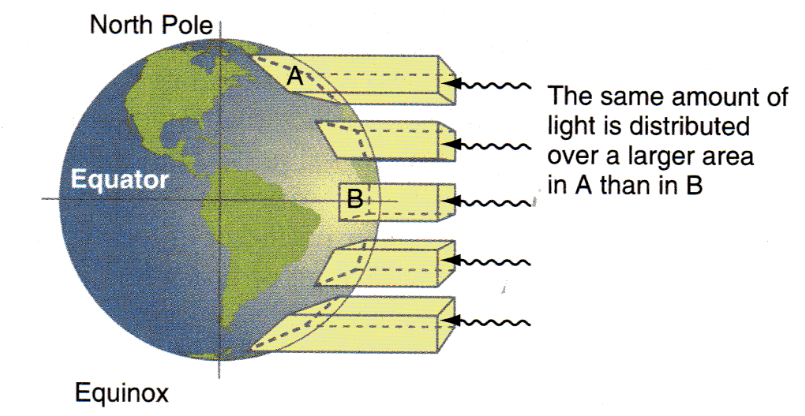
\includegraphics[width=0.6\textwidth]{sunlight.png}
    \caption[Sunlight towards Earth at the equinox]{Sunlight towards Earth at the equinox~\cite{ackerman2007meteorology}}
    \label{fig:sunlight_png}
\end{figure}


\subsection*{Power conversion}

From this solar energy, solar cells generate a current which is proportional to the illuminance. Most of the solar cell datasheets provide an IV curve at a fixed illuminance of $\SI{1}{sun} = \SI{1e3}{W/m^2}$. Since $\SI{1}{lux} = \SI{0.0079}{W/m^2}$ for the solar spectrum, the harvested current $I_\te{cell}(t)$ from one solar cell is given by
\[
  \frac{I_\te{cell}(t)}{L_\te{sun}(t)} = \frac{I_{1\te{sun}}}{1} \quad \Rightarrow \quad I_\te{cell}(t) = I_{1\te{sun}}\,L_\te{sun}(t) = \SI{0.0079e-3}{}\,I_{1\te{sun}}\,L(t) \quad \si{[A]}
\]
where $L(t)$ and $L_{\te{sun}}(t)$ are the instantaneous illuminance (resp. expressed in lux and sun) and $I_{1\te{sun}}$ is the current generated at the MPP under \SI{1}{sun} (provided in the datasheet).

\begin{figure}[H]
    \centering
    % This file was created by matlab2tikz.
%
%The latest updates can be retrieved from
%  http://www.mathworks.com/matlabcentral/fileexchange/22022-matlab2tikz-matlab2tikz
%where you can also make suggestions and rate matlab2tikz.
%
\definecolor{mycolor1}{rgb}{0.00000,0.44700,0.74100}%
%
\begin{tikzpicture}[scale=0.7]

\begin{axis}[%
width=4.521in,
height=1.6in,
at={(0.758in,0.481in)},
scale only axis,
xmin=0,
xmax=25,
xlabel style={font=\color{white!15!black}},
xlabel={Time [hours]},
ymin=0,
ymax=8,
ylabel style={font=\color{white!15!black}},
ylabel={Harvested power [mW]},
axis background/.style={fill=white},
xmajorgrids,
ymajorgrids
]
\addplot [color=mycolor1, line width=2.0pt, forget plot]
  table[row sep=crcr]{%
0	0\\
0.00873163854654635	0\\
0.0174632770930927	0\\
0.026194915639639	0\\
0.0349265541861854	0\\
0.0436581927327317	0\\
0.0523898312792781	0\\
0.0611214698258244	0\\
0.0698531083723708	0\\
0.0785847469189171	0\\
0.0873163854654635	0\\
0.0960480240120098	0\\
0.104779662558556	0\\
0.113511301105103	0\\
0.122242939651649	0\\
0.130974578198195	0\\
0.139706216744742	0\\
0.148437855291288	0\\
0.157169493837834	0\\
0.165901132384381	0\\
0.174632770930927	0\\
0.183364409477473	0\\
0.19209604802402	0\\
0.200827686570566	0\\
0.209559325117112	0\\
0.218290963663659	0\\
0.227022602210205	0\\
0.235754240756751	0\\
0.244485879303298	0\\
0.253217517849844	0\\
0.26194915639639	0\\
0.270680794942937	0\\
0.279412433489483	0\\
0.28814407203603	0\\
0.296875710582576	0\\
0.305607349129122	0\\
0.314338987675669	0\\
0.323070626222215	0\\
0.331802264768761	0\\
0.340533903315308	0\\
0.349265541861854	0\\
0.3579971804084	0\\
0.366728818954947	0\\
0.375460457501493	0\\
0.384192096048039	0\\
0.392923734594586	0\\
0.401655373141132	0\\
0.410387011687678	0\\
0.419118650234225	0\\
0.427850288780771	0\\
0.436581927327317	0\\
0.445313565873864	0\\
0.45404520442041	0\\
0.462776842966957	0\\
0.471508481513503	0\\
0.480240120060049	0\\
0.488971758606596	0\\
0.497703397153142	0\\
0.506435035699688	0\\
0.515166674246235	0\\
0.523898312792781	0\\
0.532629951339327	0\\
0.541361589885874	0\\
0.55009322843242	0\\
0.558824866978966	0\\
0.567556505525513	0\\
0.576288144072059	0\\
0.585019782618605	0\\
0.593751421165152	0\\
0.602483059711698	0\\
0.611214698258244	0\\
0.619946336804791	0\\
0.628677975351337	0\\
0.637409613897884	0\\
0.64614125244443	0\\
0.654872890990976	0\\
0.663604529537523	0\\
0.672336168084069	0\\
0.681067806630615	0\\
0.689799445177162	0\\
0.698531083723708	0\\
0.707262722270254	0\\
0.715994360816801	0\\
0.724725999363347	0\\
0.733457637909893	0\\
0.74218927645644	0\\
0.750920915002986	0\\
0.759652553549532	0\\
0.768384192096079	0\\
0.777115830642625	0\\
0.785847469189171	0\\
0.794579107735718	0\\
0.803310746282264	0\\
0.812042384828811	0\\
0.820774023375357	0\\
0.829505661921903	0\\
0.83823730046845	0\\
0.846968939014996	0\\
0.855700577561542	0\\
0.864432216108089	0\\
0.873163854654635	0\\
0.881895493201181	0\\
0.890627131747728	0\\
0.899358770294274	0\\
0.90809040884082	0\\
0.916822047387367	0\\
0.925553685933913	0\\
0.934285324480459	0\\
0.943016963027006	0\\
0.951748601573552	0\\
0.960480240120098	0\\
0.969211878666645	0\\
0.977943517213191	0\\
0.986675155759738	0\\
0.995406794306284	0\\
1.00413843285283	0\\
1.01287007139938	0\\
1.02160170994592	0\\
1.03033334849247	0\\
1.03906498703902	0\\
1.04779662558556	0\\
1.05652826413211	0\\
1.06525990267865	0\\
1.0739915412252	0\\
1.08272317977175	0\\
1.09145481831829	0\\
1.10018645686484	0\\
1.10891809541139	0\\
1.11764973395793	0\\
1.12638137250448	0\\
1.13511301105103	0\\
1.14384464959757	0\\
1.15257628814412	0\\
1.16130792669066	0\\
1.17003956523721	0\\
1.17877120378376	0\\
1.1875028423303	0\\
1.19623448087685	0\\
1.2049661194234	0\\
1.21369775796994	0\\
1.22242939651649	0\\
1.23116103506304	0\\
1.23989267360958	0\\
1.24862431215613	0\\
1.25735595070267	0\\
1.26608758924922	0\\
1.27481922779577	0\\
1.28355086634231	0\\
1.29228250488886	0\\
1.30101414343541	0\\
1.30974578198195	0\\
1.3184774205285	0\\
1.32720905907505	0\\
1.33594069762159	0\\
1.34467233616814	0\\
1.35340397471468	0\\
1.36213561326123	0\\
1.37086725180778	0\\
1.37959889035432	0\\
1.38833052890087	0\\
1.39706216744742	0\\
1.40579380599396	0\\
1.41452544454051	0\\
1.42325708308706	0\\
1.4319887216336	0\\
1.44072036018015	0\\
1.44945199872669	0\\
1.45818363727324	0\\
1.46691527581979	0\\
1.47564691436633	0\\
1.48437855291288	0\\
1.49311019145943	0\\
1.50184183000597	0\\
1.51057346855252	0\\
1.51930510709906	0\\
1.52803674564561	0\\
1.53676838419216	0\\
1.5455000227387	0\\
1.55423166128525	0\\
1.5629632998318	0\\
1.57169493837834	0\\
1.58042657692489	0\\
1.58915821547144	0\\
1.59788985401798	0\\
1.60662149256453	0\\
1.61535313111107	0\\
1.62408476965762	0\\
1.63281640820417	0\\
1.64154804675071	0\\
1.65027968529726	0\\
1.65901132384381	0\\
1.66774296239035	0\\
1.6764746009369	0\\
1.68520623948345	0\\
1.69393787802999	0\\
1.70266951657654	0\\
1.71140115512308	0\\
1.72013279366963	0\\
1.72886443221618	0\\
1.73759607076272	0\\
1.74632770930927	0\\
1.75505934785582	0\\
1.76379098640236	0\\
1.77252262494891	0\\
1.78125426349546	0\\
1.789985902042	0\\
1.79871754058855	0\\
1.80744917913509	0\\
1.81618081768164	0\\
1.82491245622819	0\\
1.83364409477473	0\\
1.84237573332128	0\\
1.85110737186783	0\\
1.85983901041437	0\\
1.86857064896092	0\\
1.87730228750747	0\\
1.88603392605401	0\\
1.89476556460056	0\\
1.9034972031471	0\\
1.91222884169365	0\\
1.9209604802402	0\\
1.92969211878674	0\\
1.93842375733329	0\\
1.94715539587984	0\\
1.95588703442638	0\\
1.96461867297293	0\\
1.97335031151948	0\\
1.98208195006602	0\\
1.99081358861257	0\\
1.99954522715911	0\\
2.00827686570566	0\\
2.01700850425221	0\\
2.02574014279875	0\\
2.0344717813453	0\\
2.04320341989185	0\\
2.05193505843839	0\\
2.06066669698494	0\\
2.06939833553148	0\\
2.07812997407803	0\\
2.08686161262458	0\\
2.09559325117112	0\\
2.10432488971767	0\\
2.11305652826422	0\\
2.12178816681076	0\\
2.13051980535731	0\\
2.13925144390386	0\\
2.1479830824504	0\\
2.15671472099695	0\\
2.16544635954349	0\\
2.17417799809004	0\\
2.18290963663659	0\\
2.19164127518313	0\\
2.20037291372968	0\\
2.20910455227623	0\\
2.21783619082277	0\\
2.22656782936932	0\\
2.23529946791587	0\\
2.24403110646241	0\\
2.25276274500896	0\\
2.2614943835555	0\\
2.27022602210205	0\\
2.2789576606486	0\\
2.28768929919514	0\\
2.29642093774169	0\\
2.30515257628824	0\\
2.31388421483478	0\\
2.32261585338133	0\\
2.33134749192788	0\\
2.34007913047442	0\\
2.34881076902097	0\\
2.35754240756751	0\\
2.36627404611406	0\\
2.37500568466061	0\\
2.38373732320715	0\\
2.3924689617537	0\\
2.40120060030025	0\\
2.40993223884679	0\\
2.41866387739334	0\\
2.42739551593989	0\\
2.43612715448643	0\\
2.44485879303298	0\\
2.45359043157952	0\\
2.46232207012607	0\\
2.47105370867262	0\\
2.47978534721916	0\\
2.48851698576571	0\\
2.49724862431226	0\\
2.5059802628588	0\\
2.51471190140535	0\\
2.5234435399519	0\\
2.53217517849844	0\\
2.54090681704499	0\\
2.54963845559153	0\\
2.55837009413808	0\\
2.56710173268463	0\\
2.57583337123117	0\\
2.58456500977772	0\\
2.59329664832427	0\\
2.60202828687081	0\\
2.61075992541736	0\\
2.6194915639639	0\\
2.62822320251045	0\\
2.636954841057	0\\
2.64568647960354	0\\
2.65441811815009	0\\
2.66314975669664	0\\
2.67188139524318	0\\
2.68061303378973	0\\
2.68934467233628	0\\
2.69807631088282	0\\
2.70680794942937	0\\
2.71553958797591	0\\
2.72427122652246	0\\
2.73300286506901	0\\
2.74173450361555	0\\
2.7504661421621	0\\
2.75919778070865	0\\
2.76792941925519	0\\
2.77666105780174	0\\
2.78539269634829	0\\
2.79412433489483	0\\
2.80285597344138	0\\
2.81158761198792	0\\
2.82031925053447	0\\
2.82905088908102	0\\
2.83778252762756	0\\
2.84651416617411	0\\
2.85524580472066	0\\
2.8639774432672	0\\
2.87270908181375	0\\
2.8814407203603	0\\
2.89017235890684	0\\
2.89890399745339	0\\
2.90763563599993	0\\
2.91636727454648	0\\
2.92509891309303	0\\
2.93383055163957	0\\
2.94256219018612	0\\
2.95129382873267	0\\
2.96002546727921	0\\
2.96875710582576	0\\
2.97748874437231	0\\
2.98622038291885	0\\
2.9949520214654	0\\
3.00368366001194	0\\
3.01241529855849	0\\
3.02114693710504	0\\
3.02987857565158	0\\
3.03861021419813	0\\
3.04734185274468	0\\
3.05607349129122	0\\
3.06480512983777	0\\
3.07353676838432	0\\
3.08226840693086	0\\
3.09100004547741	0\\
3.09973168402395	0\\
3.1084633225705	0\\
3.11719496111705	0\\
3.12592659966359	0\\
3.13465823821014	0\\
3.14338987675669	0\\
3.15212151530323	0\\
3.16085315384978	0\\
3.16958479239632	0\\
3.17831643094287	0\\
3.18704806948942	0\\
3.19577970803596	0\\
3.20451134658251	0\\
3.21324298512906	0\\
3.2219746236756	0\\
3.23070626222215	0\\
3.2394379007687	0\\
3.24816953931524	0\\
3.25690117786179	0\\
3.26563281640833	0\\
3.27436445495488	0\\
3.28309609350143	0\\
3.29182773204797	0\\
3.30055937059452	0\\
3.30929100914107	0\\
3.31802264768761	0\\
3.32675428623416	0\\
3.33548592478071	0\\
3.34421756332725	0\\
3.3529492018738	0\\
3.36168084042034	0\\
3.37041247896689	0\\
3.37914411751344	0\\
3.38787575605998	0\\
3.39660739460653	0\\
3.40533903315308	0\\
3.41407067169962	0\\
3.42280231024617	0\\
3.43153394879272	0\\
3.44026558733926	0\\
3.44899722588581	0\\
3.45772886443235	0\\
3.4664605029789	0\\
3.47519214152545	0\\
3.48392378007199	0\\
3.49265541861854	0\\
3.50138705716509	0\\
3.51011869571163	0\\
3.51885033425818	0\\
3.52758197280473	0\\
3.53631361135127	0\\
3.54504524989782	0\\
3.55377688844436	0\\
3.56250852699091	0\\
3.57124016553746	0\\
3.579971804084	0\\
3.58870344263055	0\\
3.5974350811771	0\\
3.60616671972364	0\\
3.61489835827019	0\\
3.62362999681674	0\\
3.63236163536328	0\\
3.64090909090909	0\\
3.64964072945564	0\\
3.65837236800218	0\\
3.66710400654873	0\\
3.67583564509527	0\\
3.68456728364182	0\\
3.69329892218837	0\\
3.70203056073491	0\\
3.71076219928146	0\\
3.719493837828	0\\
3.72822547637455	0\\
3.7369571149211	0\\
3.74568875346764	0\\
3.75442039201419	0\\
3.76315203056073	0\\
3.77188366910728	0\\
3.78061530765383	0\\
3.78934694620037	0\\
3.79807858474692	0\\
3.80681022329346	0\\
3.81554186184001	0\\
3.82427350038656	0\\
3.8330051389331	0\\
3.84173677747965	0\\
3.85046841602619	0\\
3.85920005457274	0\\
3.86793169311929	0\\
3.87666333166583	0\\
3.88539497021238	0\\
3.89412660875892	0\\
3.90285824730547	0\\
3.91158988585202	0\\
3.92032152439856	0\\
3.92905316294511	0\\
3.93778480149165	0\\
3.9465164400382	0\\
3.95524807858475	0\\
3.96397971713129	0\\
3.97271135567784	0\\
3.98144299422438	0\\
3.99017463277093	0\\
3.99890627131748	0\\
4.00763790986402	0\\
4.01636954841057	0\\
4.02510118695711	0\\
4.03383282550366	0\\
4.04256446405021	0\\
4.05129610259675	0\\
4.0600277411433	0\\
4.06875937968984	0\\
4.07749101823639	0\\
4.08622265678294	0\\
4.09495429532948	0\\
4.10368593387603	0\\
4.11241757242257	0\\
4.12114921096912	0\\
4.12988084951567	0\\
4.13861248806221	0\\
4.14734412660876	0\\
4.1560757651553	0\\
4.16480740370185	0\\
4.1735390422484	0\\
4.18227068079494	0\\
4.19100231934149	0\\
4.19973395788804	0\\
4.20846559643458	0\\
4.21719723498113	0\\
4.22592887352767	0\\
4.23466051207422	0\\
4.24339215062077	0\\
4.25212378916731	0\\
4.26085542771386	0\\
4.2695870662604	0\\
4.27831870480695	0\\
4.2870503433535	0\\
4.29578198190004	0\\
4.30451362044659	0\\
4.31324525899313	0\\
4.32197689753968	0\\
4.33070853608622	0\\
4.33944017463277	0\\
4.34817181317932	0\\
4.35690345172586	0\\
4.36563509027241	0\\
4.37436672881895	0\\
4.3830983673655	0\\
4.39183000591205	0\\
4.40056164445859	0\\
4.40929328300514	0\\
4.41802492155168	0\\
4.42675656009823	0\\
4.43548819864478	0\\
4.44421983719132	0\\
4.45295147573787	0\\
4.46168311428441	0\\
4.47041475283096	0\\
4.47914639137751	0\\
4.48787802992405	0\\
4.4966096684706	0\\
4.50534130701714	0\\
4.51407294556369	0\\
4.52280458411024	0\\
4.53153622265678	0\\
4.54026786120333	0\\
4.54899949974988	0\\
4.55773113829642	0\\
4.56646277684297	0\\
4.57519441538951	0\\
4.58392605393606	0\\
4.59265769248261	0\\
4.60138933102915	0\\
4.6101209695757	0\\
4.61885260812224	0\\
4.62758424666879	0\\
4.63631588521534	0\\
4.64504752376188	0\\
4.65377916230843	0\\
4.66251080085497	0\\
4.67124243940152	0\\
4.67997407794807	0\\
4.68870571649461	0\\
4.69743735504116	0\\
4.7061689935877	0\\
4.71490063213425	0\\
4.72363227068079	0\\
4.73236390922734	0\\
4.74109554777389	0\\
4.74982718632043	0\\
4.75855882486698	0\\
4.76729046341352	0\\
4.77602210196007	0\\
4.78475374050662	0\\
4.79348537905316	0\\
4.80221701759971	0\\
4.81094865614625	0\\
4.8196802946928	0\\
4.82841193323935	0\\
4.83714357178589	0\\
4.84587521033244	0\\
4.85460684887899	0\\
4.86333848742553	0\\
4.87207012597208	0\\
4.88080176451862	0\\
4.88953340306517	0\\
4.89826504161172	0\\
4.90699668015826	0\\
4.91572831870481	0\\
4.92445995725135	0\\
4.9331915957979	0\\
4.94192323434445	0\\
4.95065487289099	0\\
4.95938651143754	0\\
4.96811814998408	0\\
4.97684978853063	0\\
4.98558142707718	0\\
4.99431306562372	0\\
5.00304470417027	0\\
5.01177634271681	0\\
5.02050798126336	0\\
5.02923961980991	0\\
5.03797125835645	0\\
5.046702896903	0\\
5.05543453544954	0\\
5.06416617399609	0\\
5.07289781254264	0\\
5.08162945108918	0\\
5.09036108963573	0\\
5.09909272818227	0\\
5.10782436672882	0\\
5.11655600527536	0\\
5.12528764382191	0\\
5.13401928236846	0\\
5.142750920915	0\\
5.15148255946155	0\\
5.1602141980081	0\\
5.16894583655464	0\\
5.17767747510119	0\\
5.18640911364773	0\\
5.19514075219428	0\\
5.20387239074083	0\\
5.21260402928737	0\\
5.22133566783392	0\\
5.23006730638046	0\\
5.23879894492701	0\\
5.24753058347356	0\\
5.2562622220201	0\\
5.26499386056665	0\\
5.27372549911319	0\\
5.28245713765974	0\\
5.29118877620629	0\\
5.29992041475283	0\\
5.30865205329938	0\\
5.31738369184592	0\\
5.32611533039247	0\\
5.33484696893901	0\\
5.34357860748556	0\\
5.35231024603211	0\\
5.36104188457865	0\\
5.3697735231252	0\\
5.37850516167174	0\\
5.38723680021829	0\\
5.39596843876484	0\\
5.40470007731138	0\\
5.41343171585793	0\\
5.42216335440447	0\\
5.43089499295102	0\\
5.43962663149757	0\\
5.44835827004411	0\\
5.45708990859066	0\\
5.4658215471372	0\\
5.47455318568375	0\\
5.4832848242303	0\\
5.49201646277684	0\\
5.50074810132339	0\\
5.50947973986993	0\\
5.51821137841648	0\\
5.52694301696303	0\\
5.53567465550957	0\\
5.54440629405612	0\\
5.55313793260266	0\\
5.56186957114921	0\\
5.57060120969576	0\\
5.5793328482423	0\\
5.58806448678885	0\\
5.59679612533539	0\\
5.60552776388194	0\\
5.61425940242849	0\\
5.62299104097503	0\\
5.63172267952158	0\\
5.64045431806812	0\\
5.64918595661467	0\\
5.65791759516122	0\\
5.66664923370776	0\\
5.67538087225431	0\\
5.68411251080085	0\\
5.6928441493474	0\\
5.70157578789395	0\\
5.71030742644049	0\\
5.71903906498704	0\\
5.72777070353358	0\\
5.73650234208013	0\\
5.74523398062668	0\\
5.75396561917322	0\\
5.76269725771977	0\\
5.77142889626631	0\\
5.78016053481286	0\\
5.78889217335941	0\\
5.79762381190595	0\\
5.8063554504525	0\\
5.81508708899904	0\\
5.82381872754559	0\\
5.83255036609214	0\\
5.84128200463868	0\\
5.85001364318523	0\\
5.85874528173177	0\\
5.86747692027832	0\\
5.87620855882487	0\\
5.88494019737141	0\\
5.89367183591796	0\\
5.9024034744645	0\\
5.91113511301105	0\\
5.9198667515576	0\\
5.92859839010414	0\\
5.93733002865069	0\\
5.94606166719724	0\\
5.95479330574378	0\\
5.96352494429033	0\\
5.97225658283687	0\\
5.98098822138342	0\\
5.98971985992996	0\\
5.99845149847651	0\\
6.00718313702306	0\\
6.0159147755696	0\\
6.02464641411615	0\\
6.0333780526627	0\\
6.04210969120924	0\\
6.05084132975579	0\\
6.05957296830233	0\\
6.06830460684888	0\\
6.07703624539542	0\\
6.08576788394197	0\\
6.09449952248852	0\\
6.10323116103506	0\\
6.11196279958161	0\\
6.12069443812815	0\\
6.1294260766747	0\\
6.13815771522125	0\\
6.14688935376779	0\\
6.15562099231434	0\\
6.16435263086088	0\\
6.17308426940743	0\\
6.18181590795398	0\\
6.19054754650052	0\\
6.19927918504707	0\\
6.20801082359361	0\\
6.21674246214016	0\\
6.22547410068671	0\\
6.23420573923325	0\\
6.2429373777798	0\\
6.25166901632635	0\\
6.26040065487289	0\\
6.26913229341944	0\\
6.27786393196598	0\\
6.28659557051253	0\\
6.29532720905908	0\\
6.30405884760562	0\\
6.31279048615217	0\\
6.32152212469871	0\\
6.33025376324526	0\\
6.33898540179181	0\\
6.34771704033835	0\\
6.3564486788849	0\\
6.36518031743144	0\\
6.37391195597799	0\\
6.38264359452453	0\\
6.39137523307108	0\\
6.40010687161763	0\\
6.40883851016417	0\\
6.41757014871072	0\\
6.42630178725727	0\\
6.43503342580381	0\\
6.44376506435036	0\\
6.4524967028969	0\\
6.46122834144345	0\\
6.46995997998999	0\\
6.47869161853654	0\\
6.48742325708309	0\\
6.49615489562963	0\\
6.50488653417618	0\\
6.51361817272272	0\\
6.52234981126927	0\\
6.53108144981582	0\\
6.53981308836236	0\\
6.54854472690891	0\\
6.55727636545545	0\\
6.566008004002	0\\
6.57473964254855	0\\
6.58347128109509	0\\
6.59220291964164	0\\
6.60093455818819	0\\
6.60966619673473	0\\
6.61839783528128	0\\
6.62712947382782	0\\
6.63586111237437	0\\
6.64459275092092	0\\
6.65332438946746	0\\
6.66205602801401	0\\
6.67078766656055	0\\
6.6795193051071	0\\
6.68825094365365	0\\
6.69698258220019	0\\
6.70571422074674	0\\
6.71444585929328	0\\
6.72317749783983	0\\
6.73190913638638	0\\
6.74064077493292	0\\
6.74937241347947	0\\
6.75810405202601	0\\
6.76683569057256	0\\
6.7755673291191	0\\
6.78429896766565	0\\
6.7930306062122	0\\
6.80176224475874	0\\
6.81049388330529	0\\
6.81922552185183	0\\
6.82795716039838	0\\
6.83668879894493	0\\
6.84542043749147	0\\
6.85415207603802	0\\
6.86288371458456	0\\
6.87161535313111	0\\
6.88034699167766	0\\
6.8890786302242	0\\
6.89781026877075	0\\
6.9065419073173	0\\
6.91527354586384	0\\
6.92400518441039	0\\
6.93273682295693	0\\
6.94146846150348	0\\
6.95020010005002	0\\
6.95893173859657	0\\
6.96766337714312	0\\
6.97639501568966	0\\
6.98512665423621	0\\
6.99385829278275	0\\
7.0025899313293	0\\
7.01132156987585	0\\
7.02005320842239	0\\
7.02878484696894	0\\
7.03751648551548	0\\
7.04624812406203	0\\
7.05497976260858	0\\
7.06371140115512	0\\
7.07244303970167	0\\
7.08117467824821	0\\
7.08990631679476	0\\
7.09863795534131	0\\
7.10736959388785	0\\
7.1161012324344	0\\
7.12483287098094	0\\
7.13356450952749	0\\
7.14229614807404	0\\
7.15102778662058	0\\
7.15975942516713	0\\
7.16849106371367	0\\
7.17722270226022	0\\
7.18595434080677	0\\
7.19468597935331	0\\
7.20341761789986	0\\
7.21214925644641	0\\
7.22088089499295	0\\
7.2296125335395	0\\
7.23834417208604	0\\
7.24707581063259	0\\
7.25580744917913	0\\
7.26453908772568	0\\
7.27327072627223	0\\
7.28200236481877	0\\
7.29073400336532	0\\
7.29946564191187	0\\
7.30819728045841	0\\
7.31692891900496	0\\
7.3256605575515	0\\
7.33439219609805	0\\
7.34312383464459	0\\
7.35185547319114	0\\
7.36058711173769	0\\
7.36931875028423	0\\
7.37805038883078	0\\
7.38678202737732	0\\
7.39551366592387	0\\
7.40424530447042	0\\
7.41297694301696	0\\
7.42170858156351	0\\
7.43044022011005	0\\
7.4391718586566	0\\
7.44790349720315	0\\
7.45663513574969	0\\
7.46536677429624	0\\
7.47409841284278	0\\
7.48283005138933	0\\
7.49156168993588	0\\
7.50029332848242	0\\
7.50902496702897	0\\
7.51775660557551	0\\
7.52648824412206	0\\
7.53521988266861	0\\
7.54395152121515	0\\
7.5526831597617	0\\
7.56141479830825	0\\
7.57014643685479	0\\
7.57887807540134	0\\
7.58760971394788	0\\
7.59634135249443	0\\
7.60507299104097	0\\
7.61380462958752	0\\
7.62253626813407	0\\
7.63126790668061	0\\
7.63999954522716	0\\
7.6487311837737	0\\
7.65746282232025	0\\
7.6661944608668	0\\
7.67492609941334	0\\
7.68365773795989	0\\
7.69238937650643	0\\
7.70112101505298	0\\
7.70985265359953	0\\
7.71858429214607	0\\
7.72731593069262	0\\
7.73604756923917	0\\
7.74477920778571	0\\
7.75351084633226	0\\
7.7622424848788	0\\
7.77097412342535	0\\
7.7797057619719	0\\
7.78843740051844	0\\
7.79716903906499	0\\
7.80590067761153	0\\
7.81463231615808	0\\
7.82336395470462	0\\
7.83209559325117	0\\
7.84082723179772	0\\
7.84955887034426	0\\
7.85829050889081	0\\
7.86702214743735	0\\
7.8757537859839	0\\
7.88448542453045	0\\
7.89321706307699	0\\
7.90194870162354	0\\
7.91068034017009	0\\
7.91941197871663	0\\
7.92814361726318	0\\
7.93687525580972	0\\
7.94560689435627	0\\
7.95433853290282	0\\
7.96307017144936	0\\
7.97180180999591	0\\
7.98053344854245	0\\
7.989265087089	0\\
7.99799672563555	0\\
8.00672836418209	0\\
8.01546000272864	0\\
8.02419164127518	0\\
8.03292327982173	0\\
8.04165491836827	0\\
8.05038655691482	0\\
8.05911819546137	0\\
8.06784983400791	0\\
8.07658147255446	0\\
8.08531311110101	0\\
8.09404474964755	0\\
8.1027763881941	0\\
8.11150802674064	0\\
8.12023966528719	0\\
8.12897130383374	0\\
8.13770294238028	0\\
8.14643458092683	0\\
8.15516621947337	0\\
8.16389785801992	0\\
8.17262949656646	0\\
8.18136113511301	0\\
8.19009277365956	0\\
8.1988244122061	0\\
8.20755605075265	0\\
8.21628768929919	0\\
8.22501932784574	0\\
8.23375096639229	0\\
8.24248260493883	0\\
8.25121424348538	0\\
8.25994588203192	0\\
8.26867752057847	0\\
8.27740915912502	0\\
8.28614079767156	0\\
8.29487243621811	0\\
8.30360407476465	0\\
8.3123357133112	0\\
8.32106735185775	0\\
8.32979899040429	0\\
8.33853062895084	0\\
8.34726226749738	0\\
8.35599390604393	0\\
8.36472554459048	0\\
8.37345718313702	0\\
8.38218882168357	0\\
8.39092046023011	0\\
8.39965209877666	0\\
8.40838373732321	0\\
8.41711537586975	0\\
8.4258470144163	0\\
8.43457865296284	0\\
8.44331029150939	0\\
8.45204193005594	0\\
8.46077356860248	0\\
8.46950520714903	0\\
8.47823684569557	0\\
8.48696848424212	0\\
8.49570012278867	0\\
8.50443176133521	0\\
8.51316339988176	0\\
8.5218950384283	0\\
8.53062667697485	0\\
8.5393583155214	0\\
8.54808995406794	0\\
8.55682159261449	0\\
8.56555323116103	0\\
8.57428486970758	0\\
8.58301650825413	0\\
8.59174814680067	0\\
8.60047978534722	0\\
8.60921142389376	0\\
8.61794306244031	0\\
8.62667470098686	0\\
8.6354063395334	0\\
8.64413797807995	0\\
8.65286961662649	0\\
8.66160125517304	0\\
8.67033289371959	0\\
8.67906453226613	0\\
8.68779617081268	0\\
8.69652780935922	0\\
8.70525944790577	0\\
8.71399108645232	0\\
8.72272272499886	0\\
8.73145436354541	0\\
8.74018600209195	0\\
8.7489176406385	0\\
8.75764927918505	0\\
8.76638091773159	0\\
8.77511255627814	0\\
8.78384419482468	0\\
8.79257583337123	0\\
8.80130747191778	0\\
8.81003911046432	0\\
8.81877074901087	0\\
8.82750238755742	0\\
8.83623402610396	0\\
8.84496566465051	0\\
8.85369730319705	0\\
8.8624289417436	0\\
8.87116058029014	0\\
8.87989221883669	0\\
8.88862385738324	0\\
8.89735549592978	0\\
8.90608713447633	0\\
8.91481877302287	0\\
8.92355041156942	0\\
8.93228205011597	0\\
8.94101368866251	0\\
8.94974532720906	0\\
8.9584769657556	0\\
8.96720860430215	0\\
8.9759402428487	0\\
8.98467188139524	0\\
8.99340351994179	0\\
9.00213515848834	0\\
9.01086679703488	0\\
9.01959843558143	0\\
9.02833007412797	0\\
9.03706171267452	0\\
9.04579335122106	0\\
9.05452498976761	0\\
9.06325662831416	0\\
9.0719882668607	0\\
9.08071990540725	0\\
9.08945154395379	0\\
9.09818318250034	0\\
9.10691482104689	0\\
9.11564645959343	0\\
9.12437809813998	0\\
9.13310973668652	0\\
9.14184137523307	0\\
9.15057301377962	0\\
9.15930465232616	0\\
9.16803629087271	0\\
9.17676792941926	0\\
9.1854995679658	0\\
9.19423120651235	0\\
9.20296284505889	0\\
9.21169448360544	0\\
9.22042612215198	0\\
9.22915776069853	0\\
9.23788939924508	0\\
9.24662103779162	0\\
9.25535267633817	0\\
9.26408431488472	0\\
9.27281595343126	0\\
9.28154759197781	0\\
9.29027923052435	0\\
9.2990108690709	0\\
9.30774250761744	0\\
9.31647414616399	0\\
9.32520578471054	0\\
9.33393742325708	0\\
9.34266906180363	0\\
9.35140070035017	0\\
9.36013233889672	0\\
9.36886397744327	0\\
9.37759561598981	0\\
9.38632725453636	0\\
9.3950588930829	0\\
9.40379053162945	0\\
9.412522170176	0\\
9.42125380872254	0\\
9.42998544726909	0\\
9.43871708581564	0\\
9.44744872436218	0\\
9.45618036290873	0\\
9.46491200145527	0\\
9.47364364000182	0\\
9.48237527854836	0\\
9.49110691709491	0\\
9.49983855564146	0\\
9.508570194188	0\\
9.51730183273455	0\\
9.52603347128109	0\\
9.53476510982764	0\\
9.54349674837419	0\\
9.55222838692073	0\\
9.56096002546728	0\\
9.56969166401382	0.0025048969196836\\
9.57842330256037	0.0371154758621844\\
9.58715494110692	0.0716462628891322\\
9.59588657965346	0.106097258000548\\
9.60461821820001	0.140468461196422\\
9.61334985674656	0.174759872476763\\
9.6220814952931	0.208971491841562\\
9.63081313383965	0.243103319290819\\
9.63954477238619	0.277155354824538\\
9.64827641093274	0.311127598442721\\
9.65700804947928	0.345020050145366\\
9.66573968802583	0.378832709932469\\
9.67447132657238	0.412565577804029\\
9.68320296511892	0.446218653760052\\
9.69193460366547	0.479791937800538\\
9.70066624221202	0.513285429925492\\
9.70939788075856	0.546699130134893\\
9.71812951930511	0.580033038428762\\
9.72686115785165	0.613287154807094\\
9.7355927963982	0.646461479269884\\
9.74432443494475	0.679556011817131\\
9.75305607349129	0.712570752448841\\
9.76178771203784	0.745505701165013\\
9.77051935058438	0.778360857965649\\
9.77925098913093	0.811136222850747\\
9.78798262767748	0.843831795820298\\
9.79671426622402	0.876447576874311\\
9.80544590477057	0.908983566012793\\
9.81417754331711	0.941439763235727\\
9.82290918186366	0.973816168543118\\
9.8316408204102	1.00611278193498\\
9.84037245895675	1.03832960341131\\
9.8491040975033	1.07046663297209\\
9.85783573604984	1.10252387061733\\
9.86656737459639	1.13450131634703\\
9.87529901314293	1.16639897016119\\
9.88403065168948	1.19821683205982\\
9.89276229023603	1.22995490204291\\
9.90149392878257	1.26161318011045\\
9.91022556732912	1.29319166626246\\
9.91895720587566	1.32469036049893\\
9.92768884442221	1.35610926281986\\
9.93642048296876	1.38744837322525\\
9.9451521215153	1.4187076917151\\
9.95388376006185	1.44988721828941\\
9.9626153986084	1.48098695294818\\
9.97134703715494	1.51200689569142\\
9.98007867570149	1.54294704651911\\
9.98881031424803	1.57380740543127\\
9.99754195279458	1.60458797242789\\
10.0062735913411	1.63528874750896\\
10.0150052298877	1.6659097306745\\
10.0237368684342	1.69645092192449\\
10.0324685069808	1.72691232125896\\
10.0412001455273	1.75729392867788\\
10.0499317840739	1.78759574418126\\
10.0586634226204	1.8178177677691\\
10.0673950611669	1.84795999944141\\
10.0761266997135	1.87802243919817\\
10.08485833826	1.9080050870394\\
10.0935899768066	1.93790794296508\\
10.1023216153531	1.96773100697523\\
10.1110532538997	1.99747427906983\\
10.1197848924462	2.02713775924891\\
10.1285165309928	2.05672144751244\\
10.1372481695393	2.08622534386043\\
10.1459798080859	2.11564944829288\\
10.1547114466324	2.14499376080979\\
10.163443085179	2.17425828141116\\
10.1721747237255	2.20344301009699\\
10.180906362272	2.23254794686729\\
10.1896380008186	2.26157309172205\\
10.1983696393651	2.29051844466127\\
10.2071012779117	2.31938400568494\\
10.2158329164582	2.34816977479308\\
10.2245645550048	2.37687575198568\\
10.2332961935513	2.40550193726274\\
10.2420278320979	2.43404833062425\\
10.2507594706444	2.46251493207024\\
10.259491109191	2.49090174160068\\
10.2682227477375	2.51920875921559\\
10.2769543862841	2.54743598491495\\
10.2856860248306	2.57558341869877\\
10.2944176633771	2.60365106056706\\
10.3031493019237	2.63163891051981\\
10.3118809404702	2.65954696855702\\
10.3206125790168	2.68737523467869\\
10.3293442175633	2.71512370888481\\
10.3380758561099	2.7427923911754\\
10.3468074946564	2.77038128155046\\
10.355539133203	2.79789038000997\\
10.3642707717495	2.82531968655394\\
10.3730024102961	2.85266920118238\\
10.3817340488426	2.87993892389528\\
10.3904656873891	2.90712885469263\\
10.3991973259357	2.93423899357445\\
10.4079289644822	2.96126934054072\\
10.4166606030288	2.98821989559146\\
10.4253922415753	3.01509065872667\\
10.4341238801219	3.04188162994632\\
10.4428555186684	3.06859280925045\\
10.451587157215	3.09522419663903\\
10.4603187957615	3.12177579211207\\
10.4690504343081	3.14824759566958\\
10.4777820728546	3.17463960731154\\
10.4865137114012	3.20095182703796\\
10.4952453499477	3.22718425484885\\
10.5039769884942	3.25333689074421\\
10.5127086270408	3.27940973472401\\
10.5214402655873	3.30540278678828\\
10.5301719041339	3.33131604693701\\
10.5389035426804	3.35714951517021\\
10.547635181227	3.38290319148785\\
10.5563668197735	3.40857707588997\\
10.5650984583201	3.43417116837653\\
10.5738300968666	3.45968546894757\\
10.5825617354132	3.48511997760307\\
10.5912933739597	3.51047469434303\\
10.6000250125063	3.53574961916744\\
10.6087566510528	3.56094475207632\\
10.6174882895993	3.58606009306966\\
10.6262199281459	3.61109564214746\\
10.6349515666924	3.63605139930972\\
10.643683205239	3.66092736455644\\
10.6524148437855	3.68572353788763\\
10.6611464823321	3.71043991930327\\
10.6698781208786	3.73507650880337\\
10.6786097594252	3.75963330638794\\
10.6873413979717	3.78411031205696\\
10.6960730365183	3.80850752581045\\
10.7048046750648	3.83282494764839\\
10.7135363136113	3.8570625775708\\
10.7222679521579	3.88122041557768\\
10.7309995907044	3.90529846166901\\
10.739731229251	3.9292967158448\\
10.7484628677975	3.95321517810505\\
10.7571945063441	3.97705384844976\\
10.7659261448906	4.00081272687894\\
10.7746577834372	4.02449181339257\\
10.7833894219837	4.04809110799067\\
10.7921210605303	4.07161061067323\\
10.8008526990768	4.09505032144024\\
10.8095843376234	4.11841024029173\\
10.8183159761699	4.14169036722766\\
10.8270476147164	4.16489070224806\\
10.835779253263	4.18801124535292\\
10.8445108918095	4.21105199654225\\
10.8532425303561	4.23401295581603\\
10.8619741689026	4.25689412317427\\
10.8707058074492	4.27969549861697\\
10.8794374459957	4.30241708214414\\
10.8881690845423	4.32505887375577\\
10.8969007230888	4.34762087345185\\
10.9056323616354	4.3701030812324\\
10.9143640001819	4.39250549709741\\
10.9230956387285	4.41482812104688\\
10.931827277275	4.43707095308081\\
10.9405589158215	4.4592339931992\\
10.9492905543681	4.48131724140205\\
10.9580221929146	4.50332069768937\\
10.9667538314612	4.52524436206115\\
10.9754854700077	4.54708823451738\\
10.9842171085543	4.56885231505807\\
10.9929487471008	4.59053660368324\\
11.0016803856474	4.61214110039286\\
11.0104120241939	4.63366580518693\\
11.0191436627405	4.65511071806547\\
11.027875301287	4.67647583902847\\
11.0366069398336	4.69776116807593\\
11.0453385783801	4.71896670520786\\
11.0540702169266	4.74009245042424\\
11.0628018554732	4.76113840372508\\
11.0715334940197	4.78210456511039\\
11.0802651325663	4.80299093458016\\
11.0889967711128	4.82379751213438\\
11.0977284096594	4.84452429777307\\
11.1064600482059	4.86517129149622\\
11.1151916867525	4.88573849330383\\
11.123923325299	4.90622590319589\\
11.1326549638456	4.92663352117242\\
11.1413866023921	4.94696134723341\\
11.1501182409386	4.96720938137887\\
11.1588498794852	4.98737762360878\\
11.1675815180317	5.00746607392316\\
11.1763131565783	5.027474732322\\
11.1850447951248	5.04740359880529\\
11.1937764336714	5.06725267337305\\
11.2025080722179	5.08702195602527\\
11.2112397107645	5.10671144676194\\
11.219971349311	5.12632114558309\\
11.2287029878576	5.14585105248869\\
11.2374346264041	5.16530116747875\\
11.2461662649507	5.18467149055327\\
11.2548979034972	5.20396202171226\\
11.2636295420437	5.2231727609557\\
11.2723611805903	5.24230370828361\\
11.2810928191368	5.26135486369597\\
11.2898244576834	5.28032622719279\\
11.2985560962299	5.29921779877409\\
11.3072877347765	5.31802957843984\\
11.316019373323	5.33676156619005\\
11.3247510118696	5.35541376202471\\
11.3334826504161	5.37398616594385\\
11.3422142889627	5.39247877794744\\
11.3509459275092	5.4108915980355\\
11.3596775660558	5.42922462620801\\
11.3684092046023	5.44747786246498\\
11.3771408431488	5.46565130680642\\
11.3858724816954	5.48374495923232\\
11.3946041202419	5.50175881974267\\
11.4033357587885	5.51969288833749\\
11.412067397335	5.53754716501677\\
11.4207990358816	5.55532164978051\\
11.4295306744281	5.57301634262872\\
11.4382623129747	5.59063124356137\\
11.4469939515212	5.60816635257849\\
11.4557255900678	5.62562166968008\\
11.4644572286143	5.64299719486613\\
11.4731888671609	5.66029292813663\\
11.4819205057074	5.6775088694916\\
11.4906521442539	5.69464501893103\\
11.4993837828005	5.71170137645492\\
11.508115421347	5.72867794206327\\
11.5168470598936	5.74557471575608\\
11.5255786984401	5.76239169753334\\
11.5343103369867	5.77912888739508\\
11.5430419755332	5.79578628534126\\
11.5517736140798	5.81236389137193\\
11.5605052526263	5.82886170548704\\
11.5692368911729	5.84527972768661\\
11.5779685297194	5.86161795797065\\
11.586700168266	5.87787639633914\\
11.5954318068125	5.89405504279211\\
11.604163445359	5.91015389732951\\
11.6128950839056	5.92617295995141\\
11.6216267224521	5.94211223065774\\
11.6303583609987	5.95797170944854\\
11.6390899995452	5.97375139632381\\
11.6478216380918	5.98945129128353\\
11.6565532766383	6.00507139432771\\
11.6652849151849	6.02061170545636\\
11.6740165537314	6.03607222466947\\
11.682748192278	6.05145295196703\\
11.6914798308245	6.06675388734906\\
11.700211469371	6.08197503081555\\
11.7089431079176	6.0971163823665\\
11.7176747464641	6.11217794200191\\
11.7264063850107	6.12715970972178\\
11.7351380235572	6.14206168552612\\
11.7438696621038	6.1568838694149\\
11.7526013006503	6.17162626138816\\
11.7613329391969	6.18628886144587\\
11.7700645777434	6.20087166958805\\
11.77879621629	6.21537468581468\\
11.7875278548365	6.22979791012578\\
11.7962594933831	6.24414134252134\\
11.8049911319296	6.25840498300136\\
11.8137227704761	6.27258883156584\\
11.8224544090227	6.28669288821478\\
11.8311860475692	6.30071715294819\\
11.8399176861158	6.31466162576605\\
11.8486493246623	6.32852630666837\\
11.8573809632089	6.34231119565515\\
11.8661126017554	6.35601629272639\\
11.874844240302	6.36964159788211\\
11.8835758788485	6.38318711112227\\
11.8923075173951	6.3966528324469\\
11.9010391559416	6.41003876185599\\
11.9097707944882	6.42334489934955\\
11.9185024330347	6.43657124492755\\
11.9272340715812	6.44971779859002\\
11.9359657101278	6.46278456033695\\
11.9446973486743	6.47577153016835\\
11.9534289872209	6.4886787080842\\
11.9621606257674	6.50150609408452\\
11.970892264314	6.51425368816929\\
11.9796239028605	6.52692149033853\\
11.9883555414071	6.53950950059222\\
11.9970871799536	6.55201771893039\\
12.0058188185002	6.56444614535301\\
12.0145504570467	6.57679477986009\\
12.0232820955933	6.58906362245163\\
12.0320137341398	6.60125267312762\\
12.0407453726863	6.6133619318881\\
12.0494770112329	6.62539139873302\\
12.0582086497794	6.63734107366241\\
12.066940288326	6.64921095667625\\
12.0756719268725	6.66100104777456\\
12.0844035654191	6.67271134695732\\
12.0931352039656	6.68434185422456\\
12.1018668425122	6.69589256957624\\
12.1105984810587	6.70736349301238\\
12.1193301196053	6.71875462453301\\
12.1280617581518	6.73006596413808\\
12.1367933966983	6.74129751182761\\
12.1455250352449	6.7524492676016\\
12.1542566737914	6.76352123146006\\
12.162988312338	6.77451340340297\\
12.1717199508845	6.78542578343035\\
12.1804515894311	6.79625837154219\\
12.1891832279776	6.80701116773848\\
12.1979148665242	6.81768417201924\\
12.2066465050707	6.82827738438446\\
12.2153781436173	6.83879080483415\\
12.2241097821638	6.84922443336828\\
12.2328414207104	6.85957826998689\\
12.2415730592569	6.86985231468995\\
12.2503046978034	6.88004656747747\\
12.25903633635	6.89016102834946\\
12.2677679748965	6.9001956973059\\
12.2764996134431	6.91015057434682\\
12.2852312519896	6.92002565947218\\
12.2939628905362	6.92982095268201\\
12.3026945290827	6.9395364539763\\
12.3114261676293	6.94917216335505\\
12.3201578061758	6.95872808081826\\
12.3288894447224	6.96820420636593\\
12.3376210832689	6.97760053999806\\
12.3463527218155	6.98691708171466\\
12.355084360362	6.99615383151572\\
12.3638159989085	7.00531078940123\\
12.3725476374551	7.0143879553712\\
12.3812792760016	7.02338532942564\\
12.3900109145482	7.03230291156455\\
12.3987425530947	7.0411407017879\\
12.4074741916413	7.04989870009572\\
12.4162058301878	7.058576906488\\
12.4249374687344	7.06717532096475\\
12.4336691072809	7.07569394352594\\
12.4424007458275	7.08413277417161\\
12.451132384374	7.09249181290174\\
12.4598640229206	7.10077105971632\\
12.4685956614671	7.10897051461537\\
12.4773273000136	7.11709017759888\\
12.4860589385602	7.12513004866685\\
12.4947905771067	7.13309012781927\\
12.5035222156533	7.14097041505616\\
12.5122538541998	7.14877091037751\\
12.5209854927464	7.15649161378333\\
12.5297171312929	7.1641325252736\\
12.5384487698395	7.17169364484834\\
12.547180408386	7.17917497250752\\
12.5559120469326	7.18657650825119\\
12.5646436854791	7.19389825207929\\
12.5733753240256	7.20114020399187\\
12.5821069625722	7.20830236398891\\
12.5908386011187	7.21538473207041\\
12.5995702396653	7.22238730823638\\
12.6083018782118	7.22931009248679\\
12.6170335167584	7.23615308482167\\
12.6257651553049	7.24291628524102\\
12.6344967938515	7.24959969374482\\
12.643228432398	7.25620331033308\\
12.6519600709446	7.26272713500581\\
12.6606917094911	7.269171167763\\
12.6694233480377	7.27553540860464\\
12.6781549865842	7.28181985753075\\
12.6868866251307	7.28802451454132\\
12.6956182636773	7.29414937963635\\
12.7043499022238	7.30019445281584\\
12.7130815407704	7.30615973407979\\
12.7218131793169	7.3120452234282\\
12.7305448178635	7.31785092086107\\
12.73927645641	7.32357682637841\\
12.7480080949566	7.3292229399802\\
12.7567397335031	7.33478926166646\\
12.7654713720497	7.34027579143717\\
12.7742030105962	7.34568252929235\\
12.7829346491428	7.35100947523199\\
12.7916662876893	7.35625662925608\\
12.8003979262358	7.36142399136465\\
12.8091295647824	7.36651156155767\\
12.8178612033289	7.37151933983515\\
12.8265928418755	7.37644732619709\\
12.835324480422	7.3812955206435\\
12.8440561189686	7.38606392317436\\
12.8527877575151	7.39075253378968\\
12.8615193960617	7.39536135248947\\
12.8702510346082	7.39989037927372\\
12.8789826731548	7.40433961414243\\
12.8877143117013	7.40870905709559\\
12.8964459502479	7.41299870813322\\
12.9051775887944	7.41720856725532\\
12.9139092273409	7.42133863446187\\
12.9226408658875	7.42538890975288\\
12.931372504434	7.42935939312835\\
12.9401041429806	7.43325008458829\\
12.9488357815271	7.43706098413268\\
12.9575674200737	7.44079209176155\\
12.9662990586202	7.44444340747486\\
12.9750306971668	7.44801493127263\\
12.9837623357133	7.45150666315488\\
12.9924939742599	7.45491860312157\\
13.0012256128064	7.45825075117273\\
13.0099572513529	7.46150310730835\\
13.0186888898995	7.46467567152844\\
13.027420528446	7.46776844383297\\
13.0361521669926	7.47078142422199\\
13.0448838055391	7.47371461269545\\
13.0536154440857	7.47656800925337\\
13.0623470826322	7.47934161389576\\
13.0710787211788	7.4820354266226\\
13.0798103597253	7.48464944743392\\
13.0885419982719	7.48718367632968\\
13.0972736368184	7.48963811330992\\
13.106005275365	7.4920127583746\\
13.1147369139115	7.49430761152375\\
13.123468552458	7.49652267275737\\
13.1322001910046	7.49865794207544\\
13.1409318295511	7.50071341947798\\
13.1496634680977	7.50268910496497\\
13.1583951066442	7.50458499853644\\
13.1671267451908	7.50640110019234\\
13.1758583837373	7.50813740993273\\
13.1845900222839	7.50979392775756\\
13.1933216608304	7.51137065366686\\
13.202053299377	7.51286758766063\\
13.2107849379235	7.51428472973885\\
13.2195165764701	7.51562207990153\\
13.2282482150166	7.51687963814867\\
13.2369798535631	7.51805740448027\\
13.2457114921097	7.51915537889634\\
13.2544431306562	7.52017356139687\\
13.2631747692028	7.52111195198185\\
13.2719064077493	7.52197055065131\\
13.2806380462959	7.52274935740522\\
13.2893696848424	7.52344837224358\\
13.298101323389	7.52406759516641\\
13.3068329619355	7.5246070261737\\
13.3155646004821	7.52506666526545\\
13.3242962390286	7.52544651244167\\
13.3330278775752	7.52574656770233\\
13.3417595161217	7.52596683104748\\
13.3504911546682	7.52610730247707\\
13.3592227932148	7.52616798199113\\
13.3679544317613	7.52614886958965\\
13.3766860703079	7.52604996527262\\
13.3854177088544	7.52587126904006\\
13.394149347401	7.52561278089196\\
13.4028809859475	7.52527450082832\\
13.4116126244941	7.52485642884914\\
13.4203442630406	7.52435856495443\\
13.4290759015872	7.52378090914417\\
13.4378075401337	7.52312346141837\\
13.4465391786802	7.52238622177704\\
13.4552708172268	7.52156919022016\\
13.4640024557733	7.52067236674776\\
13.4727340943199	7.5196957513598\\
13.4814657328664	7.51863934405632\\
13.490197371413	7.51750314483728\\
13.4989290099595	7.51628715370272\\
13.5076606485061	7.5149913706526\\
13.5163922870526	7.51361579568695\\
13.5251239255992	7.51216042880577\\
13.5338555641457	7.51062527000904\\
13.5425872026923	7.50901031929678\\
13.5513188412388	7.50731557666897\\
13.5600504797853	7.50554104212563\\
13.5687821183319	7.50368671566675\\
13.5775137568784	7.50175259729233\\
13.586245395425	7.49973868700237\\
13.5949770339715	7.49764498479687\\
13.6037086725181	7.49547149067583\\
13.6124403110646	7.49321820463925\\
13.6211719496112	7.49088512668714\\
13.6299035881577	7.48847225681948\\
13.6386352267043	7.48597959503629\\
13.6473668652508	7.48340714133755\\
13.6560985037974	7.48075489572328\\
13.6648301423439	7.47802285819347\\
13.6735617808904	7.47521102874811\\
13.682293419437	7.47231940738722\\
13.6910250579835	7.46934799411079\\
13.6997566965301	7.46629678891881\\
13.7084883350766	7.46316579181131\\
13.7172199736232	7.45995500278827\\
13.7259516121697	7.45666442184968\\
13.7346832507163	7.45329404899555\\
13.7434148892628	7.44984388422589\\
13.7521465278094	7.44631392754069\\
13.7608781663559	7.44270417893994\\
13.7696098049025	7.43901463842367\\
13.778341443449	7.43524530599183\\
13.7870730819955	7.43139618164448\\
13.7958047205421	7.42746726538158\\
13.8045363590886	7.42345855720315\\
13.8132679976352	7.41937005710916\\
13.8219996361817	7.41520176509965\\
13.8307312747283	7.4109536811746\\
13.8394629132748	7.406625805334\\
13.8481945518214	7.40221813757786\\
13.8569261903679	7.39773067790618\\
13.8656578289145	7.39316342631898\\
13.874389467461	7.38851638281623\\
13.8831211060075	7.38378954739794\\
13.8918527445541	7.37898292006411\\
13.9005843831006	7.37409650081475\\
13.9093160216472	7.36913028964983\\
13.9180476601937	7.36408428656938\\
13.9267792987403	7.3589584915734\\
13.9355109372868	7.35375290466187\\
13.9442425758334	7.34846752583481\\
13.9529742143799	7.34310235509221\\
13.9617058529265	7.33765739243406\\
13.970437491473	7.33213263786038\\
13.9791691300196	7.32652809137116\\
13.9879007685661	7.3208437529664\\
13.9966324071126	7.3150796226461\\
14.0053640456592	7.30923570041027\\
14.0140956842057	7.30331198625888\\
14.0228273227523	7.29730848019197\\
14.0315589612988	7.29122518220951\\
14.0402905998454	7.28506209231152\\
14.0490222383919	7.27881921049798\\
14.0577538769385	7.27249653676891\\
14.066485515485	7.2660940711243\\
14.0752171540316	7.25961181356416\\
14.0839487925781	7.25304976408847\\
14.0926804311247	7.24640792269723\\
14.1014120696712	7.23968628939046\\
14.1101437082177	7.23288486416816\\
14.1188753467643	7.22600364703031\\
14.1276069853108	7.21904263797693\\
14.1363386238574	7.212001837008\\
14.1450702624039	7.20488124412354\\
14.1538019009505	7.19768085932353\\
14.162533539497	7.19040068260799\\
14.1712651780436	7.18304071397691\\
14.1799968165901	7.17560095343028\\
14.1887284551367	7.16808140096813\\
14.1974600936832	7.16048205659043\\
14.2061917322298	7.1528029202972\\
14.2149233707763	7.14504399208841\\
14.2236550093228	7.13720527196411\\
14.2323866478694	7.12928675992425\\
14.2411182864159	7.12128845596885\\
14.2498499249625	7.11321036009792\\
14.258581563509	7.10505247231144\\
14.2673132020556	7.09681479260943\\
14.2760448406021	7.08849732099189\\
14.2847764791487	7.0801000574588\\
14.2935081176952	7.07162300201016\\
14.3022397562418	7.06306615464599\\
14.3109713947883	7.05442951536629\\
14.3197030333349	7.04571308417104\\
14.3284346718814	7.03691686106026\\
14.3371663104279	7.02804084603393\\
14.3458979489745	7.01908503909207\\
14.354629587521	7.01004944023467\\
14.3633612260676	7.00093404946173\\
14.3720928646141	6.99173886677325\\
14.3808245031607	6.98246389216923\\
14.3895561417072	6.97310912564966\\
14.3982877802538	6.96367456721456\\
14.4070194188003	6.95416021686393\\
14.4157510573469	6.94456607459776\\
14.4244826958934	6.93489214041605\\
14.4332143344399	6.92513841431878\\
14.4419459729865	6.91530489630599\\
14.450677611533	6.90539158637766\\
14.4594092500796	6.89539848453378\\
14.4681408886261	6.88532559077437\\
14.4768725271727	6.87517290509942\\
14.4856041657192	6.86494042750894\\
14.4943358042658	6.8546281580029\\
14.5030674428123	6.84423609658133\\
14.5117990813589	6.83376424324423\\
14.5205307199054	6.82321259799158\\
14.529262358452	6.8125811608234\\
14.5379939969985	6.80186993173968\\
14.546725635545	6.79107891074041\\
14.5554572740916	6.78020809782562\\
14.5641889126381	6.76925749299527\\
14.5729205511847	6.75822709624939\\
14.5816521897312	6.74711690758796\\
14.5903838282778	6.73592692701101\\
14.5991154668243	6.72465715451851\\
14.6078471053709	6.71330759011047\\
14.6165787439174	6.7018782337869\\
14.625310382464	6.69036908554779\\
14.6340420210105	6.67878014539313\\
14.6427736595571	6.66711141332293\\
14.6515052981036	6.65536288933721\\
14.6602369366501	6.64353457343593\\
14.6689685751967	6.63162646561913\\
14.6777002137432	6.61963856588677\\
14.6864318522898	6.60757087423889\\
14.6951634908363	6.59542339067545\\
14.7038951293829	6.58319611519648\\
14.7126267679294	6.57088904780198\\
14.721358406476	6.55850218849193\\
14.7300900450225	6.54603553726636\\
14.7388216835691	6.53348909412522\\
14.7475533221156	6.52086285906856\\
14.7562849606621	6.50815683209635\\
14.7650165992087	6.49537101320862\\
14.7737482377552	6.48250540240534\\
14.7824798763018	6.46955999968651\\
14.7912115148483	6.45653480505217\\
14.7999431533949	6.44342981850226\\
14.8086747919414	6.43024504003683\\
14.817406430488	6.41698046965584\\
14.8261380690345	6.40363610735934\\
14.8348697075811	6.39021195314728\\
14.8436013461276	6.3767080070197\\
14.8523329846742	6.36312426897656\\
14.8610646232207	6.34946073901787\\
14.8697962617672	6.33571741714367\\
14.8785279003138	6.32189430335393\\
14.8872595388603	6.30799139764864\\
14.8959911774069	6.29400870002781\\
14.9047228159534	6.27994621049145\\
14.9134544545	6.26580392903954\\
14.9221860930465	6.25158185567208\\
14.9309177315931	6.23727999038911\\
14.9396493701396	6.22289833319058\\
14.9483810086862	6.20843688407652\\
14.9571126472327	6.19389564304692\\
14.9658442857793	6.17927461010178\\
14.9745759243258	6.1645737852411\\
14.9833075628723	6.14979316846487\\
14.9920392014189	6.13493275977312\\
15.0007708399654	6.11999255916582\\
15.009502478512	6.10497256664299\\
15.0182341170585	6.08987278220461\\
15.0269657556051	6.0746932058507\\
15.0356973941516	6.05943383758125\\
15.0444290326982	6.04409467739625\\
15.0531606712447	6.02867572529573\\
15.0618923097913	6.01317698127964\\
15.0706239483378	5.99759844534805\\
15.0793555868844	5.98194011750089\\
15.0880872254309	5.96620199773821\\
15.0968188639774	5.95038408605998\\
15.105550502524	5.9344863824662\\
15.1142821410705	5.9185088869569\\
15.1230137796171	5.90245159953205\\
15.1317454181636	5.88631452019167\\
15.1404770567102	5.87009764893574\\
15.1492086952567	5.85380098576429\\
15.1579403338033	5.83742453067728\\
15.1666719723498	5.82096828367475\\
15.1754036108964	5.80443224475666\\
15.1841352494429	5.78781641392304\\
15.1928668879894	5.77112079117389\\
15.201598526536	5.75434537650919\\
15.2103301650825	5.73749016992896\\
15.2190618036291	5.72055517143317\\
15.2277934421756	5.70354038102187\\
15.2365250807222	5.68644579869501\\
15.2452567192687	5.66927142445261\\
15.2539883578153	5.65201725829469\\
15.2627199963618	5.63468330022121\\
15.2714516349084	5.61726955023221\\
15.2801832734549	5.59977600832765\\
15.2889149120015	5.58220267450757\\
15.297646550548	5.56454954877194\\
15.3063781890945	5.54681663112077\\
15.3151098276411	5.52900392155407\\
15.3238414661876	5.51111142007182\\
15.3325731047342	5.49313912667404\\
15.3413047432807	5.47508704136072\\
15.3500363818273	5.45695516413186\\
15.3587680203738	5.43874349498746\\
15.3674996589204	5.42045203392752\\
15.3762312974669	5.40208078095204\\
15.3849629360135	5.38362973606102\\
15.39369457456	5.36509889925447\\
15.4024262131066	5.34648827053236\\
15.4111578516531	5.32779784989473\\
15.4198894901996	5.30902763734155\\
15.4286211287462	5.29017763287284\\
15.4373527672927	5.27124783648858\\
15.4460844058393	5.25223824818879\\
15.4548160443858	5.23314886797346\\
15.4635476829324	5.21397969584259\\
15.4722793214789	5.19473073179618\\
15.4810109600255	5.17540197583423\\
15.489742598572	5.15599342795675\\
15.4984742371186	5.13650508816372\\
15.5072058756651	5.11693695645515\\
15.5159375142117	5.09728903283105\\
15.5246691527582	5.07756131729141\\
15.5334007913047	5.05775380983622\\
15.5421324298513	5.03786651046549\\
15.5508640683978	5.01789941917924\\
15.5595957069444	4.99785253597743\\
15.5683273454909	4.97772586086009\\
15.5770589840375	4.95751939382722\\
15.585790622584	4.9372331348788\\
15.5945222611306	4.91686708401485\\
15.6032538996771	4.89642124123534\\
15.6119855382237	4.87589560654031\\
15.6207171767702	4.85529017992973\\
15.6294488153167	4.83460496140362\\
15.6381804538633	4.81383995096197\\
15.6469120924098	4.79299514860478\\
15.6556437309564	4.77207055433205\\
15.6643753695029	4.75106616814378\\
15.6731070080495	4.72998199003997\\
15.681838646596	4.70881802002062\\
15.6905702851426	4.68757425808574\\
15.6993019236891	4.66625070423531\\
15.7080335622357	4.64484735846934\\
15.7167652007822	4.62336422078784\\
15.7254968393288	4.60180129119078\\
15.7342284778753	4.58015856967821\\
15.7429601164218	4.55843605625008\\
15.7516917549684	4.53663375090642\\
15.7604233935149	4.51475165364722\\
15.7691550320615	4.49278976447248\\
15.777886670608	4.47074808338221\\
15.7866183091546	4.44862661037639\\
15.7953499477011	4.42642534545503\\
15.8040815862477	4.40414428861813\\
15.8128132247942	4.3817834398657\\
15.8215448633408	4.35934279919773\\
15.8302765018873	4.33682236661421\\
15.8390081404339	4.31422214211516\\
15.8477397789804	4.29154212570057\\
15.8564714175269	4.26878231737044\\
15.8652030560735	4.24594271712476\\
15.87393469462	4.22302332496357\\
15.8826663331666	4.20002414088681\\
15.8913979717131	4.17694516489452\\
15.9001296102597	4.15378639698669\\
15.9088612488062	4.13054783716333\\
15.9175928873528	4.10722948542442\\
15.9263245258993	4.08383134176998\\
15.9350561644459	4.0603534062\\
15.9437878029924	4.03679567871448\\
15.952519441539	4.01315815931342\\
15.9612510800855	3.98944084799682\\
15.969982718632	3.96564374476468\\
15.9787143571786	3.941766849617\\
15.9874459957251	3.91781016255379\\
15.9961776342717	3.89377368357503\\
16.0049092728182	3.86965741268074\\
16.0136409113648	3.8454613498709\\
16.0223725499113	3.82118549514553\\
16.0311041884579	3.79682984850461\\
16.0398358270044	3.77239440994816\\
16.048567465551	3.74787917947617\\
16.0572991040975	3.72328415708864\\
16.066030742644	3.69860934278556\\
16.0747623811906	3.67385473656696\\
16.0834940197371	3.64902033843281\\
16.0922256582837	3.62410614838313\\
16.1009572968302	3.5991121664179\\
16.1096889353768	3.57403839253713\\
16.1184205739233	3.54888482674083\\
16.1271522124699	3.52365146902899\\
16.1358838510164	3.4983383194016\\
16.144615489563	3.47294537785869\\
16.1533471281095	3.44747264440023\\
16.1620787666561	3.42192011902623\\
16.1708104052026	3.39628780173669\\
16.1795420437491	3.37057569253161\\
16.1882736822957	3.34478379141098\\
16.1970053208422	3.31891209837484\\
16.2057369593888	3.29296061342313\\
16.2144685979353	3.26692933655591\\
16.2232002364819	3.24081826777312\\
16.2319318750284	3.21462740707481\\
16.240663513575	3.18835675446096\\
16.2493951521215	3.16200630993157\\
16.2581267906681	3.13557607348664\\
16.2668584292146	3.10906604512617\\
16.2755900677612	3.08247622485017\\
16.2843217063077	3.05580661265862\\
16.2930533448542	3.02905720855153\\
16.3017849834008	3.00222801252891\\
16.3105166219473	2.97531902459074\\
16.3192482604939	2.94833024473704\\
16.3279798990404	2.92126167296779\\
16.336711537587	2.89411330928302\\
16.3454431761335	2.86688515368269\\
16.3541748146801	2.83957720616684\\
16.3629064532266	2.81218946673543\\
16.3716380917732	2.78472193538849\\
16.3803697303197	2.75717461212601\\
16.3891013688662	2.72954749694799\\
16.3978330074128	2.70184058985444\\
16.4065646459593	2.67405389084535\\
16.4152962845059	2.64618739992072\\
16.4240279230524	2.61824111708054\\
16.432759561599	2.59021504232483\\
16.4414912001455	2.56210917565358\\
16.4502228386921	2.53392351706679\\
16.4589544772386	2.50565806656446\\
16.4676861157852	2.47731282414659\\
16.4764177543317	2.44888778981318\\
16.4851493928783	2.42038296356424\\
16.4938810314248	2.39179834539975\\
16.5026126699713	2.36313393531973\\
16.5113443085179	2.33438973332415\\
16.5200759470644	2.30556573941306\\
16.528807585611	2.27666195358641\\
16.5375392241575	2.24767837584424\\
16.5462708627041	2.2186150061865\\
16.5550025012506	2.18947184461325\\
16.5637341397972	2.16024889112445\\
16.5724657783437	2.13094614572011\\
16.5811974168903	2.10156360840024\\
16.5899290554368	2.07210127916482\\
16.5986606939834	2.04255915801386\\
16.6073923325299	2.01293724494737\\
16.6161239710764	1.98323553996534\\
16.624855609623	1.95345404306776\\
16.6335872481695	1.92359275425465\\
16.6423188867161	1.89365167352601\\
16.6510505252626	1.86363080088181\\
16.6597821638092	1.83353013632208\\
16.6685138023557	1.8033496798468\\
16.6772454409023	1.77308943145601\\
16.6859770794488	1.74274939114965\\
16.6947087179954	1.71232955892777\\
16.7034403565419	1.68182993479034\\
16.7121719950885	1.65125051873738\\
16.720903633635	1.62059131076887\\
16.7296352721815	1.58985231088483\\
16.7383669107281	1.55903351908525\\
16.7470985492746	1.52813493537014\\
16.7558301878212	1.49715655973947\\
16.7645618263677	1.46609839219328\\
16.7732934649143	1.43496043273154\\
16.7820251034608	1.40374268135426\\
16.7907567420074	1.37244513806145\\
16.7994883805539	1.34106780285309\\
16.8082200191005	1.30961067572919\\
16.816951657647	1.27807375668977\\
16.8256832961936	1.24645704573478\\
16.8344149347401	1.21476054286427\\
16.8431465732866	1.18298424807824\\
16.8518782118332	1.15112816137664\\
16.8606098503797	1.11919228275952\\
16.8693414889263	1.08717661222684\\
16.8780731274728	1.05508114977864\\
16.8868047660194	1.02290589541488\\
16.8955364045659	0.9906508491356\\
16.9042680431125	0.958316010940775\\
16.912999681659	0.925901380830417\\
16.9217313202056	0.893406958804511\\
16.9304629587521	0.860832744863074\\
16.9391945972986	0.828178739006089\\
16.9479262358452	0.795444941233572\\
16.9566578743917	0.762631351545512\\
16.9653895129383	0.729737969941916\\
16.9741211514848	0.696764796422777\\
16.9828527900314	0.6637118309881\\
16.9915844285779	0.630579073637871\\
17.0003160671245	0.597366524372131\\
17.009047705671	0.564074183190828\\
17.0177793442176	0.530702050093997\\
17.0265109827641	0.497250125081619\\
17.0352426213107	0.463718408153715\\
17.0439742598572	0.430106899310263\\
17.0527058984037	0.396415598551273\\
17.0614375369503	0.362644505876747\\
17.0701691754968	0.328793621286678\\
17.0789008140434	0.294862944781071\\
17.0876324525899	0.260852476359928\\
17.0963640911365	0.226762216023242\\
17.105095729683	0.192592163771019\\
17.1138273682296	0.158342319603254\\
17.1225590067761	0.124012683519956\\
17.1312906453227	0.0896032555211006\\
17.1400222838692	0.0551140356067343\\
17.1487539224158	0.020545023776799\\
17.1574855609623	0\\
17.1662171995088	0\\
17.1749488380554	0\\
17.1836804766019	0\\
17.1924121151485	0\\
17.201143753695	0\\
17.2098753922416	0\\
17.2186070307881	0\\
17.2273386693347	0\\
17.2360703078812	0\\
17.2448019464278	0\\
17.2535335849743	0\\
17.2622652235209	0\\
17.2709968620674	0\\
17.2797285006139	0\\
17.2884601391605	0\\
17.297191777707	0\\
17.3059234162536	0\\
17.3146550548001	0\\
17.3233866933467	0\\
17.3321183318932	0\\
17.3408499704398	0\\
17.3495816089863	0\\
17.3583132475329	0\\
17.3670448860794	0\\
17.3757765246259	0\\
17.3845081631725	0\\
17.393239801719	0\\
17.4019714402656	0\\
17.4107030788121	0\\
17.4194347173587	0\\
17.4281663559052	0\\
17.4368979944518	0\\
17.4456296329983	0\\
17.4543612715449	0\\
17.4630929100914	0\\
17.471824548638	0\\
17.4805561871845	0\\
17.489287825731	0\\
17.4980194642776	0\\
17.5067511028241	0\\
17.5154827413707	0\\
17.5242143799172	0\\
17.5329460184638	0\\
17.5416776570103	0\\
17.5504092955569	0\\
17.5591409341034	0\\
17.56787257265	0\\
17.5766042111965	0\\
17.5853358497431	0\\
17.5940674882896	0\\
17.6027991268361	0\\
17.6115307653827	0\\
17.6202624039292	0\\
17.6289940424758	0\\
17.6377256810223	0\\
17.6464573195689	0\\
17.6551889581154	0\\
17.663920596662	0\\
17.6726522352085	0\\
17.6813838737551	0\\
17.6901155123016	0\\
17.6988471508481	0\\
17.7075787893947	0\\
17.7163104279412	0\\
17.7250420664878	0\\
17.7337737050343	0\\
17.7425053435809	0\\
17.7512369821274	0\\
17.759968620674	0\\
17.7687002592205	0\\
17.7774318977671	0\\
17.7861635363136	0\\
17.7948951748602	0\\
17.8036268134067	0\\
17.8123584519533	0\\
17.8210900904998	0\\
17.8298217290463	0\\
17.8385533675929	0\\
17.8472850061394	0\\
17.856016644686	0\\
17.8647482832325	0\\
17.8734799217791	0\\
17.8822115603256	0\\
17.8909431988722	0\\
17.8996748374187	0\\
17.9084064759653	0\\
17.9171381145118	0\\
17.9258697530583	0\\
17.9346013916049	0\\
17.9433330301514	0\\
17.952064668698	0\\
17.9607963072445	0\\
17.9695279457911	0\\
17.9782595843376	0\\
17.9869912228842	0\\
17.9957228614307	0\\
18.0044544999773	0\\
18.0131861385238	0\\
18.0219177770704	0\\
18.0306494156169	0\\
18.0393810541634	0\\
18.04811269271	0\\
18.0568443312565	0\\
18.0655759698031	0\\
18.0743076083496	0\\
18.0830392468962	0\\
18.0917708854427	0\\
18.1005025239893	0\\
18.1092341625358	0\\
18.1179658010824	0\\
18.1266974396289	0\\
18.1354290781755	0\\
18.144160716722	0\\
18.1528923552685	0\\
18.1616239938151	0\\
18.1703556323616	0\\
18.1790872709082	0\\
18.1878189094547	0\\
18.1965505480013	0\\
18.2052821865478	0\\
18.2140138250944	0\\
18.2227454636409	0\\
18.2314771021875	0\\
18.240208740734	0\\
18.2489403792805	0\\
18.2576720178271	0\\
18.2664036563736	0\\
18.2751352949202	0\\
18.2838669334667	0\\
18.2925985720133	0\\
18.3013302105598	0\\
18.3100618491064	0\\
18.3187934876529	0\\
18.3275251261995	0\\
18.336256764746	0\\
18.3449884032926	0\\
18.3537200418391	0\\
18.3624516803856	0\\
18.3711833189322	0\\
18.3799149574787	0\\
18.3886465960253	0\\
18.3973782345718	0\\
18.4061098731184	0\\
18.4148415116649	0\\
18.4235731502115	0\\
18.432304788758	0\\
18.4410364273046	0\\
18.4497680658511	0\\
18.4584997043977	0\\
18.4672313429442	0\\
18.4759629814907	0\\
18.4846946200373	0\\
18.4934262585838	0\\
18.5021578971304	0\\
18.5108895356769	0\\
18.5196211742235	0\\
18.52835281277	0\\
18.5370844513166	0\\
18.5458160898631	0\\
18.5545477284097	0\\
18.5632793669562	0\\
18.5720110055028	0\\
18.5807426440493	0\\
18.5894742825958	0\\
18.5982059211424	0\\
18.6069375596889	0\\
18.6156691982355	0\\
18.624400836782	0\\
18.6331324753286	0\\
18.6418641138751	0\\
18.6505957524217	0\\
18.6593273909682	0\\
18.6680590295148	0\\
18.6767906680613	0\\
18.6855223066079	0\\
18.6942539451544	0\\
18.7029855837009	0\\
18.7117172222475	0\\
18.720448860794	0\\
18.7291804993406	0\\
18.7379121378871	0\\
18.7466437764337	0\\
18.7553754149802	0\\
18.7641070535268	0\\
18.7728386920733	0\\
18.7815703306199	0\\
18.7903019691664	0\\
18.7990336077129	0\\
18.8077652462595	0\\
18.816496884806	0\\
18.8252285233526	0\\
18.8339601618991	0\\
18.8426918004457	0\\
18.8514234389922	0\\
18.8601550775388	0\\
18.8688867160853	0\\
18.8776183546319	0\\
18.8863499931784	0\\
18.895081631725	0\\
18.9038132702715	0\\
18.912544908818	0\\
18.9212765473646	0\\
18.9300081859111	0\\
18.9387398244577	0\\
18.9474714630042	0\\
18.9562031015508	0\\
18.9649347400973	0\\
18.9736663786439	0\\
18.9823980171904	0\\
18.991129655737	0\\
18.9998612942835	0\\
19.0085929328301	0\\
19.0173245713766	0\\
19.0260562099231	0\\
19.0347878484697	0\\
19.0435194870162	0\\
19.0522511255628	0\\
19.0609827641093	0\\
19.0697144026559	0\\
19.0784460412024	0\\
19.087177679749	0\\
19.0959093182955	0\\
19.1046409568421	0\\
19.1133725953886	0\\
19.1221042339351	0\\
19.1308358724817	0\\
19.1395675110282	0\\
19.1482991495748	0\\
19.1570307881213	0\\
19.1657624266679	0\\
19.1744940652144	0\\
19.183225703761	0\\
19.1919573423075	0\\
19.2006889808541	0\\
19.2094206194006	0\\
19.2181522579472	0\\
19.2268838964937	0\\
19.2356155350402	0\\
19.2443471735868	0\\
19.2530788121333	0\\
19.2618104506799	0\\
19.2705420892264	0\\
19.279273727773	0\\
19.2880053663195	0\\
19.2967370048661	0\\
19.3054686434126	0\\
19.3142002819592	0\\
19.3229319205057	0\\
19.3316635590523	0\\
19.3403951975988	0\\
19.3491268361453	0\\
19.3578584746919	0\\
19.3665901132384	0\\
19.375321751785	0\\
19.3840533903315	0\\
19.3927850288781	0\\
19.4015166674246	0\\
19.4102483059712	0\\
19.4189799445177	0\\
19.4277115830643	0\\
19.4364432216108	0\\
19.4451748601574	0\\
19.4539064987039	0\\
19.4626381372504	0\\
19.471369775797	0\\
19.4801014143435	0\\
19.4888330528901	0\\
19.4975646914366	0\\
19.5062963299832	0\\
19.5150279685297	0\\
19.5237596070763	0\\
19.5324912456228	0\\
19.5412228841694	0\\
19.5499545227159	0\\
19.5586861612625	0\\
19.567417799809	0\\
19.5761494383555	0\\
19.5848810769021	0\\
19.5936127154486	0\\
19.6023443539952	0\\
19.6110759925417	0\\
19.6198076310883	0\\
19.6285392696348	0\\
19.6372709081814	0\\
19.6460025467279	0\\
19.6547341852745	0\\
19.663465823821	0\\
19.6721974623675	0\\
19.6809291009141	0\\
19.6896607394606	0\\
19.6983923780072	0\\
19.7071240165537	0\\
19.7158556551003	0\\
19.7245872936468	0\\
19.7333189321934	0\\
19.7420505707399	0\\
19.7507822092865	0\\
19.759513847833	0\\
19.7682454863796	0\\
19.7769771249261	0\\
19.7857087634726	0\\
19.7944404020192	0\\
19.8031720405657	0\\
19.8119036791123	0\\
19.8206353176588	0\\
19.8293669562054	0\\
19.8380985947519	0\\
19.8468302332985	0\\
19.855561871845	0\\
19.8642935103916	0\\
19.8730251489381	0\\
19.8817567874847	0\\
19.8904884260312	0\\
19.8992200645777	0\\
19.9079517031243	0\\
19.9166833416708	0\\
19.9254149802174	0\\
19.9341466187639	0\\
19.9428782573105	0\\
19.951609895857	0\\
19.9603415344036	0\\
19.9690731729501	0\\
19.9778048114967	0\\
19.9865364500432	0\\
19.9952680885898	0\\
20.0039997271363	0\\
20.0127313656828	0\\
20.0214630042294	0\\
20.0301946427759	0\\
20.0389262813225	0\\
20.047657919869	0\\
20.0563895584156	0\\
20.0651211969621	0\\
20.0738528355087	0\\
20.0825844740552	0\\
20.0913161126018	0\\
20.1000477511483	0\\
20.1087793896948	0\\
20.1175110282414	0\\
20.1262426667879	0\\
20.1349743053345	0\\
20.143705943881	0\\
20.1524375824276	0\\
20.1611692209741	0\\
20.1699008595207	0\\
20.1786324980672	0\\
20.1873641366138	0\\
20.1960957751603	0\\
20.2048274137069	0\\
20.2135590522534	0\\
20.2222906907999	0\\
20.2310223293465	0\\
20.239753967893	0\\
20.2484856064396	0\\
20.2572172449861	0\\
20.2659488835327	0\\
20.2746805220792	0\\
20.2834121606258	0\\
20.2921437991723	0\\
20.3008754377189	0\\
20.3096070762654	0\\
20.318338714812	0\\
20.3270703533585	0\\
20.335801991905	0\\
20.3445336304516	0\\
20.3532652689981	0\\
20.3619969075447	0\\
20.3707285460912	0\\
20.3794601846378	0\\
20.3881918231843	0\\
20.3969234617309	0\\
20.4056551002774	0\\
20.414386738824	0\\
20.4231183773705	0\\
20.431850015917	0\\
20.4405816544636	0\\
20.4493132930101	0\\
20.4580449315567	0\\
20.4667765701032	0\\
20.4755082086498	0\\
20.4842398471963	0\\
20.4929714857429	0\\
20.5017031242894	0\\
20.510434762836	0\\
20.5191664013825	0\\
20.5278980399291	0\\
20.5366296784756	0\\
20.5453613170221	0\\
20.5540929555687	0\\
20.5628245941152	0\\
20.5715562326618	0\\
20.5802878712083	0\\
20.5890195097549	0\\
20.5977511483014	0\\
20.606482786848	0\\
20.6152144253945	0\\
20.6239460639411	0\\
20.6326777024876	0\\
20.6414093410342	0\\
20.6501409795807	0\\
20.6588726181272	0\\
20.6676042566738	0\\
20.6763358952203	0\\
20.6850675337669	0\\
20.6937991723134	0\\
20.70253081086	0\\
20.7112624494065	0\\
20.7199940879531	0\\
20.7287257264996	0\\
20.7374573650462	0\\
20.7461890035927	0\\
20.7549206421393	0\\
20.7636522806858	0\\
20.7723839192323	0\\
20.7811155577789	0\\
20.7898471963254	0\\
20.798578834872	0\\
20.8073104734185	0\\
20.8160421119651	0\\
20.8247737505116	0\\
20.8335053890582	0\\
20.8422370276047	0\\
20.8509686661513	0\\
20.8597003046978	0\\
20.8684319432443	0\\
20.8771635817909	0\\
20.8858952203374	0\\
20.894626858884	0\\
20.9033584974305	0\\
20.9120901359771	0\\
20.9208217745236	0\\
20.9295534130702	0\\
20.9382850516167	0\\
20.9470166901633	0\\
20.9557483287098	0\\
20.9644799672564	0\\
20.9732116058029	0\\
20.9819432443494	0\\
20.990674882896	0\\
20.9994065214425	0\\
21.0081381599891	0\\
21.0168697985356	0\\
21.0256014370822	0\\
21.0343330756287	0\\
21.0430647141753	0\\
21.0517963527218	0\\
21.0605279912684	0\\
21.0692596298149	0\\
21.0779912683615	0\\
21.086722906908	0\\
21.0954545454545	0\\
21.1041861840011	0\\
21.1129178225476	0\\
21.1216494610942	0\\
21.1303810996407	0\\
21.1391127381873	0\\
21.1478443767338	0\\
21.1565760152804	0\\
21.1653076538269	0\\
21.1740392923735	0\\
21.18277093092	0\\
21.1915025694666	0\\
21.2002342080131	0\\
21.2089658465596	0\\
21.2176974851062	0\\
21.2264291236527	0\\
21.2351607621993	0\\
21.2438924007458	0\\
21.2526240392924	0\\
21.2613556778389	0\\
21.2700873163855	0\\
21.278818954932	0\\
21.2875505934786	0\\
21.2962822320251	0\\
21.3050138705717	0\\
21.3137455091182	0\\
21.3224771476647	0\\
21.3312087862113	0\\
21.3399404247578	0\\
21.3486720633044	0\\
21.3574037018509	0\\
21.3661353403975	0\\
21.374866978944	0\\
21.3835986174906	0\\
21.3923302560371	0\\
21.4010618945837	0\\
21.4097935331302	0\\
21.4185251716768	0\\
21.4272568102233	0\\
21.4359884487699	0\\
21.4447200873164	0\\
21.4534517258629	0\\
21.4621833644095	0\\
21.470915002956	0\\
21.4796466415026	0\\
21.4883782800491	0\\
21.4971099185957	0\\
21.5058415571422	0\\
21.5145731956888	0\\
21.5233048342353	0\\
21.5320364727819	0\\
21.5407681113284	0\\
21.549499749875	0\\
21.5582313884215	0\\
21.566963026968	0\\
21.5756946655146	0\\
21.5844263040611	0\\
21.5931579426077	0\\
21.6018895811542	0\\
21.6106212197008	0\\
21.6193528582473	0\\
21.6280844967939	0\\
21.6368161353404	0\\
21.645547773887	0\\
21.6542794124335	0\\
21.6630110509801	0\\
21.6717426895266	0\\
21.6804743280731	0\\
21.6892059666197	0\\
21.6979376051662	0\\
21.7066692437128	0\\
21.7154008822593	0\\
21.7241325208059	0\\
21.7328641593524	0\\
21.741595797899	0\\
21.7503274364455	0\\
21.7590590749921	0\\
21.7677907135386	0\\
21.7765223520852	0\\
21.7852539906317	0\\
21.7939856291783	0\\
21.8027172677248	0\\
21.8114489062713	0\\
21.8201805448179	0\\
21.8289121833644	0\\
21.837643821911	0\\
21.8463754604575	0\\
21.8551070990041	0\\
21.8638387375506	0\\
21.8725703760972	0\\
21.8813020146437	0\\
21.8900336531903	0\\
21.8987652917368	0\\
21.9074969302834	0\\
21.9162285688299	0\\
21.9249602073764	0\\
21.933691845923	0\\
21.9424234844695	0\\
21.9511551230161	0\\
21.9598867615626	0\\
21.9686184001092	0\\
21.9773500386557	0\\
21.9860816772023	0\\
21.9948133157488	0\\
22.0035449542954	0\\
22.0122765928419	0\\
22.0210082313885	0\\
22.029739869935	0\\
22.0384715084815	0\\
22.0472031470281	0\\
22.0559347855746	0\\
22.0646664241212	0\\
22.0733980626677	0\\
22.0821297012143	0\\
22.0908613397608	0\\
22.0995929783074	0\\
22.1083246168539	0\\
22.1170562554005	0\\
22.125787893947	0\\
22.1345195324936	0\\
22.1432511710401	0\\
22.1519828095867	0\\
22.1607144481332	0\\
22.1694460866797	0\\
22.1781777252263	0\\
22.1869093637728	0\\
22.1956410023194	0\\
22.2043726408659	0\\
22.2131042794125	0\\
22.221835917959	0\\
22.2305675565056	0\\
22.2392991950521	0\\
22.2480308335987	0\\
22.2567624721452	0\\
22.2654941106918	0\\
22.2742257492383	0\\
22.2829573877848	0\\
22.2916890263314	0\\
22.3004206648779	0\\
22.3091523034245	0\\
22.317883941971	0\\
22.3266155805176	0\\
22.3353472190641	0\\
22.3440788576107	0\\
22.3528104961572	0\\
22.3615421347038	0\\
22.3702737732503	0\\
22.3790054117969	0\\
22.3877370503434	0\\
22.39646868889	0\\
22.4052003274365	0\\
22.413931965983	0\\
22.4226636045296	0\\
22.4313952430761	0\\
22.4401268816227	0\\
22.4488585201692	0\\
22.4575901587158	0\\
22.4663217972623	0\\
22.4750534358089	0\\
22.4837850743554	0\\
22.492516712902	0\\
22.5012483514485	0\\
22.5099799899951	0\\
22.5187116285416	0\\
22.5274432670881	0\\
22.5361749056347	0\\
22.5449065441812	0\\
22.5536381827278	0\\
22.5623698212743	0\\
22.5711014598209	0\\
22.5798330983674	0\\
22.588564736914	0\\
22.5972963754605	0\\
22.6060280140071	0\\
22.6147596525536	0\\
22.6234912911002	0\\
22.6322229296467	0\\
22.6409545681932	0\\
22.6496862067398	0\\
22.6584178452863	0\\
22.6671494838329	0\\
22.6758811223794	0\\
22.684612760926	0\\
22.6933443994725	0\\
22.7020760380191	0\\
22.7108076765656	0\\
22.7195393151122	0\\
22.7282709536587	0\\
22.7370025922053	0\\
22.7457342307518	0\\
22.7544658692984	0\\
22.7631975078449	0\\
22.7719291463914	0\\
22.780660784938	0\\
22.7893924234845	0\\
22.7981240620311	0\\
22.8068557005776	0\\
22.8155873391242	0\\
22.8243189776707	0\\
22.8330506162173	0\\
22.8417822547638	0\\
22.8505138933104	0\\
22.8592455318569	0\\
22.8679771704035	0\\
22.87670880895	0\\
22.8854404474965	0\\
22.8941720860431	0\\
22.9029037245896	0\\
22.9116353631362	0\\
22.9203670016827	0\\
22.9290986402293	0\\
22.9378302787758	0\\
22.9465619173224	0\\
22.9552935558689	0\\
22.9640251944155	0\\
22.972756832962	0\\
22.9814884715086	0\\
22.9902201100551	0\\
22.9989517486016	0\\
23.0076833871482	0\\
23.0164150256947	0\\
23.0251466642413	0\\
23.0338783027878	0\\
23.0426099413344	0\\
23.0513415798809	0\\
23.0600732184275	0\\
23.068804856974	0\\
23.0775364955206	0\\
23.0862681340671	0\\
23.0949997726137	0\\
23.1037314111602	0\\
23.1124630497068	0\\
23.1211946882533	0\\
23.1299263267998	0\\
23.1386579653464	0\\
23.1473896038929	0\\
23.1561212424395	0\\
23.164852880986	0\\
23.1735845195326	0\\
23.1823161580791	0\\
23.1910477966257	0\\
23.1997794351722	0\\
23.2085110737188	0\\
23.2172427122653	0\\
23.2259743508119	0\\
23.2347059893584	0\\
23.2434376279049	0\\
23.2521692664515	0\\
23.260900904998	0\\
23.2696325435446	0\\
23.2783641820911	0\\
23.2870958206377	0\\
23.2958274591842	0\\
23.3045590977308	0\\
23.3132907362773	0\\
23.3220223748239	0\\
23.3307540133704	0\\
23.339485651917	0\\
23.3482172904635	0\\
23.35694892901	0\\
23.3656805675566	0\\
23.3744122061031	0\\
23.3831438446497	0\\
23.3918754831962	0\\
23.4006071217428	0\\
23.4093387602893	0\\
23.4180703988359	0\\
23.4268020373824	0\\
23.435533675929	0\\
23.4442653144755	0\\
23.4529969530221	0\\
23.4617285915686	0\\
23.4704602301152	0\\
23.4791918686617	0\\
23.4879235072082	0\\
23.4966551457548	0\\
23.5053867843013	0\\
23.5141184228479	0\\
23.5228500613944	0\\
23.531581699941	0\\
23.5403133384875	0\\
23.5490449770341	0\\
23.5577766155806	0\\
23.5665082541272	0\\
23.5752398926737	0\\
23.5839715312203	0\\
23.5927031697668	0\\
23.6014348083133	0\\
23.6101664468599	0\\
23.6188980854064	0\\
23.627629723953	0\\
23.6363613624995	0\\
23.6450930010461	0\\
23.6538246395926	0\\
23.6625562781392	0\\
23.6712879166857	0\\
23.6800195552323	0\\
23.6887511937788	0\\
23.6974828323254	0\\
23.7062144708719	0\\
23.7149461094184	0\\
23.723677747965	0\\
23.7324093865115	0\\
23.7411410250581	0\\
23.7498726636046	0\\
23.7586043021512	0\\
23.7673359406977	0\\
23.7760675792443	0\\
23.7847992177908	0\\
23.7935308563374	0\\
23.8022624948839	0\\
23.8109941334305	0\\
23.819725771977	0\\
23.8284574105236	0\\
23.8371890490701	0\\
23.8459206876166	0\\
23.8546523261632	0\\
23.8633839647097	0\\
23.8721156032563	0\\
23.8808472418028	0\\
23.8895788803494	0\\
23.8983105188959	0\\
23.9070421574425	0\\
23.915773795989	0\\
23.9245054345356	0\\
23.9332370730821	0\\
23.9419687116287	0\\
23.9507003501752	0\\
23.9594319887217	0\\
23.9681636272683	0\\
23.9768952658148	0\\
23.9856269043614	0\\
23.9943585429079	0\\
};
\end{axis}
\end{tikzpicture}%

    \caption{Daily view of the harvested power with SM141K06L solar cells}
    \label{fig:P_cell}
\end{figure}

For the selected solar cells, Figure~\ref{fig:P_cell} gives the harvested power throughout the day\footnote{As mentioned previously, notice that the graph is shrunk such that the day benefits from sunlight during only eight hours.}: 
\[
 P_\te{cell}(t) = I_\te{cell}(t)\,V_\te{cell} = \SI{0.0079e-3}{}\,I_{1\te{sun}}\,V_\te{cell}\,L(t) \quad \si{[W]}
\]
with $V_\te{cell} = \SI{3.35}{V}$ and $I_{1\te{sun}} = \SI{55.1}{mA}$.

\subsection*{Charge of the supercapacitor}

The next paragraphs will discuss how the power management unit transforms the input and output powers with two different voltage regulators.

The input power charging the supercapacitor from the solar cells is independent from the supercapacitor voltage. Indeed, the voltage at the maximum power point is converted to the supercap voltage through a boost converter with efficiency $\eta_\te{boost,PMU}=\SI{92}{\%}$ derived in Section~\ref{section:PMU}. The input power is thus
\[
 P_\te{in,solar}(t) = n_\te{¢ell} \, I_\te{cell}(t)\,V_\te{cell} = \frac{1}{\eta_\te{boost,PMU}} I_\te{in,SC}(t) \, V_\te{SC}(t) \quad [\si{W}]
\]
where $n_\te{¢ell}$ is the number of solar cells required for the device, $I_\te{in,SC}(t)$ is the input current through the supercapacitor and $V_\te{SC}(t)$ is the voltage across the supercapacitor.

Regarding the power consumption, the PMU converts the supercapacitor voltage to a constant voltage $V_\te{CC}= \SI{2.5}{V}$ via a low-dropout (LDO) regulator. Neglecting the quiescent current, LDOs keep the same current while the voltage is reduced. The output power is thus reduced, this is why it is important to maintain a small dropout (voltage difference between the input and output). Hence, the output current is independent from the supercapacitor voltage and not the output power since the ratio of output power fed to the circuit over the output power actually retrieved from the supercapacitor is given by
\[
 \frac{P_\te{out,circuit}}{P_\te{out,SC}} = \frac{I_\te{out} \, V_\te{CC}}{I_\te{out} \, V_\te{SC}} = \frac{V_\te{CC}}{V_\te{SC}}.
\]

\begin{figure}[H]
    \centering
    % This file was created by matlab2tikz.
%
%The latest updates can be retrieved from
%  http://www.mathworks.com/matlabcentral/fileexchange/22022-matlab2tikz-matlab2tikz
%where you can also make suggestions and rate matlab2tikz.
%
\definecolor{mycolor1}{rgb}{0.00000,0.44700,0.74100}%
%
\begin{tikzpicture}

\begin{axis}[%
width=4.521in,
height=1.493in,
at={(0.758in,2.554in)},
scale only axis,
xmin=0,
xmax=25,
ymin=0,
ymax=60,
ylabel style={font=\color{white!15!black}},
ylabel={Input power [mW]},
axis background/.style={fill=white},
axis x line*=bottom,
axis y line*=left,
xmajorgrids,
ymajorgrids
]
\addplot [color=mycolor1, line width=2.0pt, forget plot]
  table[row sep=crcr]{%
0	0\\
0.00873163854654635	0\\
0.0174632770930927	0\\
0.026194915639639	0\\
0.0349265541861854	0\\
0.0436581927327317	0\\
0.0523898312792781	0\\
0.0611214698258244	0\\
0.0698531083723708	0\\
0.0785847469189171	0\\
0.0873163854654635	0\\
0.0960480240120098	0\\
0.104779662558556	0\\
0.113511301105103	0\\
0.122242939651649	0\\
0.130974578198195	0\\
0.139706216744742	0\\
0.148437855291288	0\\
0.157169493837834	0\\
0.165901132384381	0\\
0.174632770930927	0\\
0.183364409477473	0\\
0.19209604802402	0\\
0.200827686570566	0\\
0.209559325117112	0\\
0.218290963663659	0\\
0.227022602210205	0\\
0.235754240756751	0\\
0.244485879303298	0\\
0.253217517849844	0\\
0.26194915639639	0\\
0.270680794942937	0\\
0.279412433489483	0\\
0.28814407203603	0\\
0.296875710582576	0\\
0.305607349129122	0\\
0.314338987675669	0\\
0.323070626222215	0\\
0.331802264768761	0\\
0.340533903315308	0\\
0.349265541861854	0\\
0.3579971804084	0\\
0.366728818954947	0\\
0.375460457501493	0\\
0.384192096048039	0\\
0.392923734594586	0\\
0.401655373141132	0\\
0.410387011687678	0\\
0.419118650234225	0\\
0.427850288780771	0\\
0.436581927327317	0\\
0.445313565873864	0\\
0.45404520442041	0\\
0.462776842966957	0\\
0.471508481513503	0\\
0.480240120060049	0\\
0.488971758606596	0\\
0.497703397153142	0\\
0.506435035699688	0\\
0.515166674246235	0\\
0.523898312792781	0\\
0.532629951339327	0\\
0.541361589885874	0\\
0.55009322843242	0\\
0.558824866978966	0\\
0.567556505525513	0\\
0.576288144072059	0\\
0.585019782618605	0\\
0.593751421165152	0\\
0.602483059711698	0\\
0.611214698258244	0\\
0.619946336804791	0\\
0.628677975351337	0\\
0.637409613897884	0\\
0.64614125244443	0\\
0.654872890990976	0\\
0.663604529537523	0\\
0.672336168084069	0\\
0.681067806630615	0\\
0.689799445177162	0\\
0.698531083723708	0\\
0.707262722270254	0\\
0.715994360816801	0\\
0.724725999363347	0\\
0.733457637909893	0\\
0.74218927645644	0\\
0.750920915002986	0\\
0.759652553549532	0\\
0.768384192096079	0\\
0.777115830642625	0\\
0.785847469189171	0\\
0.794579107735718	0\\
0.803310746282264	0\\
0.812042384828811	0\\
0.820774023375357	0\\
0.829505661921903	0\\
0.83823730046845	0\\
0.846968939014996	0\\
0.855700577561542	0\\
0.864432216108089	0\\
0.873163854654635	0\\
0.881895493201181	0\\
0.890627131747728	0\\
0.899358770294274	0\\
0.90809040884082	0\\
0.916822047387367	0\\
0.925553685933913	0\\
0.934285324480459	0\\
0.943016963027006	0\\
0.951748601573552	0\\
0.960480240120098	0\\
0.969211878666645	0\\
0.977943517213191	0\\
0.986675155759738	0\\
0.995406794306284	0\\
1.00413843285283	0\\
1.01287007139938	0\\
1.02160170994592	0\\
1.03033334849247	0\\
1.03906498703902	0\\
1.04779662558556	0\\
1.05652826413211	0\\
1.06525990267865	0\\
1.0739915412252	0\\
1.08272317977175	0\\
1.09145481831829	0\\
1.10018645686484	0\\
1.10891809541139	0\\
1.11764973395793	0\\
1.12638137250448	0\\
1.13511301105103	0\\
1.14384464959757	0\\
1.15257628814412	0\\
1.16130792669066	0\\
1.17003956523721	0\\
1.17877120378376	0\\
1.1875028423303	0\\
1.19623448087685	0\\
1.2049661194234	0\\
1.21369775796994	0\\
1.22242939651649	0\\
1.23116103506304	0\\
1.23989267360958	0\\
1.24862431215613	0\\
1.25735595070267	0\\
1.26608758924922	0\\
1.27481922779577	0\\
1.28355086634231	0\\
1.29228250488886	0\\
1.30101414343541	0\\
1.30974578198195	0\\
1.3184774205285	0\\
1.32720905907505	0\\
1.33594069762159	0\\
1.34467233616814	0\\
1.35340397471468	0\\
1.36213561326123	0\\
1.37086725180778	0\\
1.37959889035432	0\\
1.38833052890087	0\\
1.39706216744742	0\\
1.40579380599396	0\\
1.41452544454051	0\\
1.42325708308706	0\\
1.4319887216336	0\\
1.44072036018015	0\\
1.44945199872669	0\\
1.45818363727324	0\\
1.46691527581979	0\\
1.47564691436633	0\\
1.48437855291288	0\\
1.49311019145943	0\\
1.50184183000597	0\\
1.51057346855252	0\\
1.51930510709906	0\\
1.52803674564561	0\\
1.53676838419216	0\\
1.5455000227387	0\\
1.55423166128525	0\\
1.5629632998318	0\\
1.57169493837834	0\\
1.58042657692489	0\\
1.58915821547144	0\\
1.59788985401798	0\\
1.60662149256453	0\\
1.61535313111107	0\\
1.62408476965762	0\\
1.63281640820417	0\\
1.64154804675071	0\\
1.65027968529726	0\\
1.65901132384381	0\\
1.66774296239035	0\\
1.6764746009369	0\\
1.68520623948345	0\\
1.69393787802999	0\\
1.70266951657654	0\\
1.71140115512308	0\\
1.72013279366963	0\\
1.72886443221618	0\\
1.73759607076272	0\\
1.74632770930927	0\\
1.75505934785582	0\\
1.76379098640236	0\\
1.77252262494891	0\\
1.78125426349546	0\\
1.789985902042	0\\
1.79871754058855	0\\
1.80744917913509	0\\
1.81618081768164	0\\
1.82491245622819	0\\
1.83364409477473	0\\
1.84237573332128	0\\
1.85110737186783	0\\
1.85983901041437	0\\
1.86857064896092	0\\
1.87730228750747	0\\
1.88603392605401	0\\
1.89476556460056	0\\
1.9034972031471	0\\
1.91222884169365	0\\
1.9209604802402	0\\
1.92969211878674	0\\
1.93842375733329	0\\
1.94715539587984	0\\
1.95588703442638	0\\
1.96461867297293	0\\
1.97335031151948	0\\
1.98208195006602	0\\
1.99081358861257	0\\
1.99954522715911	0\\
2.00827686570566	0\\
2.01700850425221	0\\
2.02574014279875	0\\
2.0344717813453	0\\
2.04320341989185	0\\
2.05193505843839	0\\
2.06066669698494	0\\
2.06939833553148	0\\
2.07812997407803	0\\
2.08686161262458	0\\
2.09559325117112	0\\
2.10432488971767	0\\
2.11305652826422	0\\
2.12178816681076	0\\
2.13051980535731	0\\
2.13925144390386	0\\
2.1479830824504	0\\
2.15671472099695	0\\
2.16544635954349	0\\
2.17417799809004	0\\
2.18290963663659	0\\
2.19164127518313	0\\
2.20037291372968	0\\
2.20910455227623	0\\
2.21783619082277	0\\
2.22656782936932	0\\
2.23529946791587	0\\
2.24403110646241	0\\
2.25276274500896	0\\
2.2614943835555	0\\
2.27022602210205	0\\
2.2789576606486	0\\
2.28768929919514	0\\
2.29642093774169	0\\
2.30515257628824	0\\
2.31388421483478	0\\
2.32261585338133	0\\
2.33134749192788	0\\
2.34007913047442	0\\
2.34881076902097	0\\
2.35754240756751	0\\
2.36627404611406	0\\
2.37500568466061	0\\
2.38373732320715	0\\
2.3924689617537	0\\
2.40120060030025	0\\
2.40993223884679	0\\
2.41866387739334	0\\
2.42739551593989	0\\
2.43612715448643	0\\
2.44485879303298	0\\
2.45359043157952	0\\
2.46232207012607	0\\
2.47105370867262	0\\
2.47978534721916	0\\
2.48851698576571	0\\
2.49724862431226	0\\
2.5059802628588	0\\
2.51471190140535	0\\
2.5234435399519	0\\
2.53217517849844	0\\
2.54090681704499	0\\
2.54963845559153	0\\
2.55837009413808	0\\
2.56710173268463	0\\
2.57583337123117	0\\
2.58456500977772	0\\
2.59329664832427	0\\
2.60202828687081	0\\
2.61075992541736	0\\
2.6194915639639	0\\
2.62822320251045	0\\
2.636954841057	0\\
2.64568647960354	0\\
2.65441811815009	0\\
2.66314975669664	0\\
2.67188139524318	0\\
2.68061303378973	0\\
2.68934467233628	0\\
2.69807631088282	0\\
2.70680794942937	0\\
2.71553958797591	0\\
2.72427122652246	0\\
2.73300286506901	0\\
2.74173450361555	0\\
2.7504661421621	0\\
2.75919778070865	0\\
2.76792941925519	0\\
2.77666105780174	0\\
2.78539269634829	0\\
2.79412433489483	0\\
2.80285597344138	0\\
2.81158761198792	0\\
2.82031925053447	0\\
2.82905088908102	0\\
2.83778252762756	0\\
2.84651416617411	0\\
2.85524580472066	0\\
2.8639774432672	0\\
2.87270908181375	0\\
2.8814407203603	0\\
2.89017235890684	0\\
2.89890399745339	0\\
2.90763563599993	0\\
2.91636727454648	0\\
2.92509891309303	0\\
2.93383055163957	0\\
2.94256219018612	0\\
2.95129382873267	0\\
2.96002546727921	0\\
2.96875710582576	0\\
2.97748874437231	0\\
2.98622038291885	0\\
2.9949520214654	0\\
3.00368366001194	0\\
3.01241529855849	0\\
3.02114693710504	0\\
3.02987857565158	0\\
3.03861021419813	0\\
3.04734185274468	0\\
3.05607349129122	0\\
3.06480512983777	0\\
3.07353676838432	0\\
3.08226840693086	0\\
3.09100004547741	0\\
3.09973168402395	0\\
3.1084633225705	0\\
3.11719496111705	0\\
3.12592659966359	0\\
3.13465823821014	0\\
3.14338987675669	0\\
3.15212151530323	0\\
3.16085315384978	0\\
3.16958479239632	0\\
3.17831643094287	0\\
3.18704806948942	0\\
3.19577970803596	0\\
3.20451134658251	0\\
3.21324298512906	0\\
3.2219746236756	0\\
3.23070626222215	0\\
3.2394379007687	0\\
3.24816953931524	0\\
3.25690117786179	0\\
3.26563281640833	0\\
3.27436445495488	0\\
3.28309609350143	0\\
3.29182773204797	0\\
3.30055937059452	0\\
3.30929100914107	0\\
3.31802264768761	0\\
3.32675428623416	0\\
3.33548592478071	0\\
3.34421756332725	0\\
3.3529492018738	0\\
3.36168084042034	0\\
3.37041247896689	0\\
3.37914411751344	0\\
3.38787575605998	0\\
3.39660739460653	0\\
3.40533903315308	0\\
3.41407067169962	0\\
3.42280231024617	0\\
3.43153394879272	0\\
3.44026558733926	0\\
3.44899722588581	0\\
3.45772886443235	0\\
3.4664605029789	0\\
3.47519214152545	0\\
3.48392378007199	0\\
3.49265541861854	0\\
3.50138705716509	0\\
3.51011869571163	0\\
3.51885033425818	0\\
3.52758197280473	0\\
3.53631361135127	0\\
3.54504524989782	0\\
3.55377688844436	0\\
3.56250852699091	0\\
3.57124016553746	0\\
3.579971804084	0\\
3.58870344263055	0\\
3.5974350811771	0\\
3.60616671972364	0\\
3.61489835827019	0\\
3.62362999681674	0\\
3.63236163536328	0\\
3.64090909090909	0\\
3.64964072945564	0\\
3.65837236800218	0\\
3.66710400654873	0\\
3.67583564509527	0\\
3.68456728364182	0\\
3.69329892218837	0\\
3.70203056073491	0\\
3.71076219928146	0\\
3.719493837828	0\\
3.72822547637455	0\\
3.7369571149211	0\\
3.74568875346764	0\\
3.75442039201419	0\\
3.76315203056073	0\\
3.77188366910728	0\\
3.78061530765383	0\\
3.78934694620037	0\\
3.79807858474692	0\\
3.80681022329346	0\\
3.81554186184001	0\\
3.82427350038656	0\\
3.8330051389331	0\\
3.84173677747965	0\\
3.85046841602619	0\\
3.85920005457274	0\\
3.86793169311929	0\\
3.87666333166583	0\\
3.88539497021238	0\\
3.89412660875892	0\\
3.90285824730547	0\\
3.91158988585202	0\\
3.92032152439856	0\\
3.92905316294511	0\\
3.93778480149165	0\\
3.9465164400382	0\\
3.95524807858475	0\\
3.96397971713129	0\\
3.97271135567784	0\\
3.98144299422438	0\\
3.99017463277093	0\\
3.99890627131748	0\\
4.00763790986402	0\\
4.01636954841057	0\\
4.02510118695711	0\\
4.03383282550366	0\\
4.04256446405021	0\\
4.05129610259675	0\\
4.0600277411433	0\\
4.06875937968984	0\\
4.07749101823639	0\\
4.08622265678294	0\\
4.09495429532948	0\\
4.10368593387603	0\\
4.11241757242257	0\\
4.12114921096912	0\\
4.12988084951567	0\\
4.13861248806221	0\\
4.14734412660876	0\\
4.1560757651553	0\\
4.16480740370185	0\\
4.1735390422484	0\\
4.18227068079494	0\\
4.19100231934149	0\\
4.19973395788804	0\\
4.20846559643458	0\\
4.21719723498113	0\\
4.22592887352767	0\\
4.23466051207422	0\\
4.24339215062077	0\\
4.25212378916731	0\\
4.26085542771386	0\\
4.2695870662604	0\\
4.27831870480695	0\\
4.2870503433535	0\\
4.29578198190004	0\\
4.30451362044659	0\\
4.31324525899313	0\\
4.32197689753968	0\\
4.33070853608622	0\\
4.33944017463277	0\\
4.34817181317932	0\\
4.35690345172586	0\\
4.36563509027241	0\\
4.37436672881895	0\\
4.3830983673655	0\\
4.39183000591205	0\\
4.40056164445859	0\\
4.40929328300514	0\\
4.41802492155168	0\\
4.42675656009823	0\\
4.43548819864478	0\\
4.44421983719132	0\\
4.45295147573787	0\\
4.46168311428441	0\\
4.47041475283096	0\\
4.47914639137751	0\\
4.48787802992405	0\\
4.4966096684706	0\\
4.50534130701714	0\\
4.51407294556369	0\\
4.52280458411024	0\\
4.53153622265678	0\\
4.54026786120333	0\\
4.54899949974988	0\\
4.55773113829642	0\\
4.56646277684297	0\\
4.57519441538951	0\\
4.58392605393606	0\\
4.59265769248261	0\\
4.60138933102915	0\\
4.6101209695757	0\\
4.61885260812224	0\\
4.62758424666879	0\\
4.63631588521534	0\\
4.64504752376188	0\\
4.65377916230843	0\\
4.66251080085497	0\\
4.67124243940152	0\\
4.67997407794807	0\\
4.68870571649461	0\\
4.69743735504116	0\\
4.7061689935877	0\\
4.71490063213425	0\\
4.72363227068079	0\\
4.73236390922734	0\\
4.74109554777389	0\\
4.74982718632043	0\\
4.75855882486698	0\\
4.76729046341352	0\\
4.77602210196007	0\\
4.78475374050662	0\\
4.79348537905316	0\\
4.80221701759971	0\\
4.81094865614625	0\\
4.8196802946928	0\\
4.82841193323935	0\\
4.83714357178589	0\\
4.84587521033244	0\\
4.85460684887899	0\\
4.86333848742553	0\\
4.87207012597208	0\\
4.88080176451862	0\\
4.88953340306517	0\\
4.89826504161172	0\\
4.90699668015826	0\\
4.91572831870481	0\\
4.92445995725135	0\\
4.9331915957979	0\\
4.94192323434445	0\\
4.95065487289099	0\\
4.95938651143754	0\\
4.96811814998408	0\\
4.97684978853063	0\\
4.98558142707718	0\\
4.99431306562372	0\\
5.00304470417027	0\\
5.01177634271681	0\\
5.02050798126336	0\\
5.02923961980991	0\\
5.03797125835645	0\\
5.046702896903	0\\
5.05543453544954	0\\
5.06416617399609	0\\
5.07289781254264	0\\
5.08162945108918	0\\
5.09036108963573	0\\
5.09909272818227	0\\
5.10782436672882	0\\
5.11655600527536	0\\
5.12528764382191	0\\
5.13401928236846	0\\
5.142750920915	0\\
5.15148255946155	0\\
5.1602141980081	0\\
5.16894583655464	0\\
5.17767747510119	0\\
5.18640911364773	0\\
5.19514075219428	0\\
5.20387239074083	0\\
5.21260402928737	0\\
5.22133566783392	0\\
5.23006730638046	0\\
5.23879894492701	0\\
5.24753058347356	0\\
5.2562622220201	0\\
5.26499386056665	0\\
5.27372549911319	0\\
5.28245713765974	0\\
5.29118877620629	0\\
5.29992041475283	0\\
5.30865205329938	0\\
5.31738369184592	0\\
5.32611533039247	0\\
5.33484696893901	0\\
5.34357860748556	0\\
5.35231024603211	0\\
5.36104188457865	0\\
5.3697735231252	0\\
5.37850516167174	0\\
5.38723680021829	0\\
5.39596843876484	0\\
5.40470007731138	0\\
5.41343171585793	0\\
5.42216335440447	0\\
5.43089499295102	0\\
5.43962663149757	0\\
5.44835827004411	0\\
5.45708990859066	0\\
5.4658215471372	0\\
5.47455318568375	0\\
5.4832848242303	0\\
5.49201646277684	0\\
5.50074810132339	0\\
5.50947973986993	0\\
5.51821137841648	0\\
5.52694301696303	0\\
5.53567465550957	0\\
5.54440629405612	0\\
5.55313793260266	0\\
5.56186957114921	0\\
5.57060120969576	0\\
5.5793328482423	0\\
5.58806448678885	0\\
5.59679612533539	0\\
5.60552776388194	0\\
5.61425940242849	0\\
5.62299104097503	0\\
5.63172267952158	0\\
5.64045431806812	0\\
5.64918595661467	0\\
5.65791759516122	0\\
5.66664923370776	0\\
5.67538087225431	0\\
5.68411251080085	0\\
5.6928441493474	0\\
5.70157578789395	0\\
5.71030742644049	0\\
5.71903906498704	0\\
5.72777070353358	0\\
5.73650234208013	0\\
5.74523398062668	0\\
5.75396561917322	0\\
5.76269725771977	0\\
5.77142889626631	0\\
5.78016053481286	0\\
5.78889217335941	0\\
5.79762381190595	0\\
5.8063554504525	0\\
5.81508708899904	0\\
5.82381872754559	0\\
5.83255036609214	0\\
5.84128200463868	0\\
5.85001364318523	0\\
5.85874528173177	0\\
5.86747692027832	0\\
5.87620855882487	0\\
5.88494019737141	0\\
5.89367183591796	0\\
5.9024034744645	0\\
5.91113511301105	0\\
5.9198667515576	0\\
5.92859839010414	0\\
5.93733002865069	0\\
5.94606166719724	0\\
5.95479330574378	0\\
5.96352494429033	0\\
5.97225658283687	0\\
5.98098822138342	0\\
5.98971985992996	0\\
5.99845149847651	0\\
6.00718313702306	0\\
6.0159147755696	0\\
6.02464641411615	0\\
6.0333780526627	0\\
6.04210969120924	0\\
6.05084132975579	0\\
6.05957296830233	0\\
6.06830460684888	0\\
6.07703624539542	0\\
6.08576788394197	0\\
6.09449952248852	0\\
6.10323116103506	0\\
6.11196279958161	0\\
6.12069443812815	0\\
6.1294260766747	0\\
6.13815771522125	0\\
6.14688935376779	0\\
6.15562099231434	0\\
6.16435263086088	0\\
6.17308426940743	0\\
6.18181590795398	0\\
6.19054754650052	0\\
6.19927918504707	0\\
6.20801082359361	0\\
6.21674246214016	0\\
6.22547410068671	0\\
6.23420573923325	0\\
6.2429373777798	0\\
6.25166901632635	0\\
6.26040065487289	0\\
6.26913229341944	0\\
6.27786393196598	0\\
6.28659557051253	0\\
6.29532720905908	0\\
6.30405884760562	0\\
6.31279048615217	0\\
6.32152212469871	0\\
6.33025376324526	0\\
6.33898540179181	0\\
6.34771704033835	0\\
6.3564486788849	0\\
6.36518031743144	0\\
6.37391195597799	0\\
6.38264359452453	0\\
6.39137523307108	0\\
6.40010687161763	0\\
6.40883851016417	0\\
6.41757014871072	0\\
6.42630178725727	0\\
6.43503342580381	0\\
6.44376506435036	0\\
6.4524967028969	0\\
6.46122834144345	0\\
6.46995997998999	0\\
6.47869161853654	0\\
6.48742325708309	0\\
6.49615489562963	0\\
6.50488653417618	0\\
6.51361817272272	0\\
6.52234981126927	0\\
6.53108144981582	0\\
6.53981308836236	0\\
6.54854472690891	0\\
6.55727636545545	0\\
6.566008004002	0\\
6.57473964254855	0\\
6.58347128109509	0\\
6.59220291964164	0\\
6.60093455818819	0\\
6.60966619673473	0\\
6.61839783528128	0\\
6.62712947382782	0\\
6.63586111237437	0\\
6.64459275092092	0\\
6.65332438946746	0\\
6.66205602801401	0\\
6.67078766656055	0\\
6.6795193051071	0\\
6.68825094365365	0\\
6.69698258220019	0\\
6.70571422074674	0\\
6.71444585929328	0\\
6.72317749783983	0\\
6.73190913638638	0\\
6.74064077493292	0\\
6.74937241347947	0\\
6.75810405202601	0\\
6.76683569057256	0\\
6.7755673291191	0\\
6.78429896766565	0\\
6.7930306062122	0\\
6.80176224475874	0\\
6.81049388330529	0\\
6.81922552185183	0\\
6.82795716039838	0\\
6.83668879894493	0\\
6.84542043749147	0\\
6.85415207603802	0\\
6.86288371458456	0\\
6.87161535313111	0\\
6.88034699167766	0\\
6.8890786302242	0\\
6.89781026877075	0\\
6.9065419073173	0\\
6.91527354586384	0\\
6.92400518441039	0\\
6.93273682295693	0\\
6.94146846150348	0\\
6.95020010005002	0\\
6.95893173859657	0\\
6.96766337714312	0\\
6.97639501568966	0\\
6.98512665423621	0\\
6.99385829278275	0\\
7.0025899313293	0\\
7.01132156987585	0\\
7.02005320842239	0\\
7.02878484696894	0\\
7.03751648551548	0\\
7.04624812406203	0\\
7.05497976260858	0\\
7.06371140115512	0\\
7.07244303970167	0\\
7.08117467824821	0\\
7.08990631679476	0\\
7.09863795534131	0\\
7.10736959388785	0\\
7.1161012324344	0\\
7.12483287098094	0\\
7.13356450952749	0\\
7.14229614807404	0\\
7.15102778662058	0\\
7.15975942516713	0\\
7.16849106371367	0\\
7.17722270226022	0\\
7.18595434080677	0\\
7.19468597935331	0\\
7.20341761789986	0\\
7.21214925644641	0\\
7.22088089499295	0\\
7.2296125335395	0\\
7.23834417208604	0\\
7.24707581063259	0\\
7.25580744917913	0\\
7.26453908772568	0\\
7.27327072627223	0\\
7.28200236481877	0\\
7.29073400336532	0\\
7.29946564191187	0\\
7.30819728045841	0\\
7.31692891900496	0\\
7.3256605575515	0\\
7.33439219609805	0\\
7.34312383464459	0\\
7.35185547319114	0\\
7.36058711173769	0\\
7.36931875028423	0\\
7.37805038883078	0\\
7.38678202737732	0\\
7.39551366592387	0\\
7.40424530447042	0\\
7.41297694301696	0\\
7.42170858156351	0\\
7.43044022011005	0\\
7.4391718586566	0\\
7.44790349720315	0\\
7.45663513574969	0\\
7.46536677429624	0\\
7.47409841284278	0\\
7.48283005138933	0\\
7.49156168993588	0\\
7.50029332848242	0\\
7.50902496702897	0\\
7.51775660557551	0\\
7.52648824412206	0\\
7.53521988266861	0\\
7.54395152121515	0\\
7.5526831597617	0\\
7.56141479830825	0\\
7.57014643685479	0\\
7.57887807540134	0\\
7.58760971394788	0\\
7.59634135249443	0\\
7.60507299104097	0\\
7.61380462958752	0\\
7.62253626813407	0\\
7.63126790668061	0\\
7.63999954522716	0\\
7.6487311837737	0\\
7.65746282232025	0\\
7.6661944608668	0\\
7.67492609941334	0\\
7.68365773795989	0\\
7.69238937650643	0\\
7.70112101505298	0\\
7.70985265359953	0\\
7.71858429214607	0\\
7.72731593069262	0\\
7.73604756923917	0\\
7.74477920778571	0\\
7.75351084633226	0\\
7.7622424848788	0\\
7.77097412342535	0\\
7.7797057619719	0\\
7.78843740051844	0\\
7.79716903906499	0\\
7.80590067761153	0\\
7.81463231615808	0\\
7.82336395470462	0\\
7.83209559325117	0\\
7.84082723179772	0\\
7.84955887034426	0\\
7.85829050889081	0\\
7.86702214743735	0\\
7.8757537859839	0\\
7.88448542453045	0\\
7.89321706307699	0\\
7.90194870162354	0\\
7.91068034017009	0\\
7.91941197871663	0\\
7.92814361726318	0\\
7.93687525580972	0\\
7.94560689435627	0\\
7.95433853290282	0\\
7.96307017144936	0\\
7.97180180999591	0\\
7.98053344854245	0\\
7.989265087089	0\\
7.99799672563555	0\\
8.00672836418209	0\\
8.01546000272864	0\\
8.02419164127518	0\\
8.03292327982173	0\\
8.04165491836827	0\\
8.05038655691482	0\\
8.05911819546137	0\\
8.06784983400791	0\\
8.07658147255446	0\\
8.08531311110101	0\\
8.09404474964755	0\\
8.1027763881941	0\\
8.11150802674064	0\\
8.12023966528719	0\\
8.12897130383374	0\\
8.13770294238028	0\\
8.14643458092683	0\\
8.15516621947337	0\\
8.16389785801992	0\\
8.17262949656646	0\\
8.18136113511301	0\\
8.19009277365956	0\\
8.1988244122061	0\\
8.20755605075265	0\\
8.21628768929919	0\\
8.22501932784574	0\\
8.23375096639229	0\\
8.24248260493883	0\\
8.25121424348538	0\\
8.25994588203192	0\\
8.26867752057847	0\\
8.27740915912502	0\\
8.28614079767156	0\\
8.29487243621811	0\\
8.30360407476465	0\\
8.3123357133112	0\\
8.32106735185775	0\\
8.32979899040429	0\\
8.33853062895084	0\\
8.34726226749738	0\\
8.35599390604393	0\\
8.36472554459048	0\\
8.37345718313702	0\\
8.38218882168357	0\\
8.39092046023011	0\\
8.39965209877666	0\\
8.40838373732321	0\\
8.41711537586975	0\\
8.4258470144163	0\\
8.43457865296284	0\\
8.44331029150939	0\\
8.45204193005594	0\\
8.46077356860248	0\\
8.46950520714903	0\\
8.47823684569557	0\\
8.48696848424212	0\\
8.49570012278867	0\\
8.50443176133521	0\\
8.51316339988176	0\\
8.5218950384283	0\\
8.53062667697485	0\\
8.5393583155214	0\\
8.54808995406794	0\\
8.55682159261449	0\\
8.56555323116103	0\\
8.57428486970758	0\\
8.58301650825413	0\\
8.59174814680067	0\\
8.60047978534722	0\\
8.60921142389376	0\\
8.61794306244031	0\\
8.62667470098686	0\\
8.6354063395334	0\\
8.64413797807995	0\\
8.65286961662649	0\\
8.66160125517304	0\\
8.67033289371959	0\\
8.67906453226613	0\\
8.68779617081268	0\\
8.69652780935922	0\\
8.70525944790577	0\\
8.71399108645232	0\\
8.72272272499886	0\\
8.73145436354541	0\\
8.74018600209195	0\\
8.7489176406385	0\\
8.75764927918505	0\\
8.76638091773159	0\\
8.77511255627814	0\\
8.78384419482468	0\\
8.79257583337123	0\\
8.80130747191778	0\\
8.81003911046432	0\\
8.81877074901087	0\\
8.82750238755742	0\\
8.83623402610396	0\\
8.84496566465051	0\\
8.85369730319705	0\\
8.8624289417436	0\\
8.87116058029014	0\\
8.87989221883669	0\\
8.88862385738324	0\\
8.89735549592978	0\\
8.90608713447633	0\\
8.91481877302287	0\\
8.92355041156942	0\\
8.93228205011597	0\\
8.94101368866251	0\\
8.94974532720906	0\\
8.9584769657556	0\\
8.96720860430215	0\\
8.9759402428487	0\\
8.98467188139524	0\\
8.99340351994179	0\\
9.00213515848834	0\\
9.01086679703488	0\\
9.01959843558143	0\\
9.02833007412797	0\\
9.03706171267452	0\\
9.04579335122106	0\\
9.05452498976761	0\\
9.06325662831416	0\\
9.0719882668607	0\\
9.08071990540725	0\\
9.08945154395379	0\\
9.09818318250034	0\\
9.10691482104689	0\\
9.11564645959343	0\\
9.12437809813998	0\\
9.13310973668652	0\\
9.14184137523307	0\\
9.15057301377962	0\\
9.15930465232616	0\\
9.16803629087271	0\\
9.17676792941926	0\\
9.1854995679658	0\\
9.19423120651235	0\\
9.20296284505889	0\\
9.21169448360544	0\\
9.22042612215198	0\\
9.22915776069853	0\\
9.23788939924508	0\\
9.24662103779162	0\\
9.25535267633817	0\\
9.26408431488472	0\\
9.27281595343126	0\\
9.28154759197781	0\\
9.29027923052435	0\\
9.2990108690709	0\\
9.30774250761744	0\\
9.31647414616399	0\\
9.32520578471054	0\\
9.33393742325708	0\\
9.34266906180363	0\\
9.35140070035017	0\\
9.36013233889672	0\\
9.36886397744327	0\\
9.37759561598981	0\\
9.38632725453636	0\\
9.3950588930829	0\\
9.40379053162945	0\\
9.412522170176	0\\
9.42125380872254	0\\
9.42998544726909	0\\
9.43871708581564	0\\
9.44744872436218	0\\
9.45618036290873	0\\
9.46491200145527	0\\
9.47364364000182	0\\
9.48237527854836	0\\
9.49110691709491	0\\
9.49983855564146	0\\
9.508570194188	0\\
9.51730183273455	0\\
9.52603347128109	0\\
9.53476510982764	0\\
9.54349674837419	0\\
9.55222838692073	0\\
9.56096002546728	0\\
9.56969166401382	0.0150293815181016\\
9.57842330256037	0.222692855173107\\
9.58715494110692	0.429877577334793\\
9.59588657965346	0.636583548003288\\
9.60461821820001	0.842810767178529\\
9.61334985674656	1.04855923486058\\
9.6220814952931	1.25382895104937\\
9.63081313383965	1.45861991574491\\
9.63954477238619	1.66293212894723\\
9.64827641093274	1.86676559065632\\
9.65700804947928	2.0701203008722\\
9.66573968802583	2.27299625959481\\
9.67447132657238	2.47539346682417\\
9.68320296511892	2.67731192256031\\
9.69193460366547	2.87875162680323\\
9.70066624221202	3.07971257955295\\
9.70939788075856	3.28019478080936\\
9.71812951930511	3.48019823057257\\
9.72686115785165	3.67972292884256\\
9.7355927963982	3.8787688756193\\
9.74432443494475	4.07733607090278\\
9.75305607349129	4.27542451469304\\
9.76178771203784	4.47303420699008\\
9.77051935058438	4.67016514779389\\
9.77925098913093	4.86681733710448\\
9.78798262767748	5.06299077492179\\
9.79671426622402	5.25868546124587\\
9.80544590477057	5.45390139607676\\
9.81417754331711	5.64863857941436\\
9.82290918186366	5.84289701125871\\
9.8316408204102	6.0366766916099\\
9.84037245895675	6.22997762046783\\
9.8491040975033	6.42279979783251\\
9.85783573604984	6.61514322370397\\
9.86656737459639	6.80700789808217\\
9.87529901314293	6.99839382096715\\
9.88403065168948	7.18930099235894\\
9.89276229023603	7.37972941225744\\
9.90149392878257	7.56967908066268\\
9.91022556732912	7.75914999757477\\
9.91895720587566	7.9481421629936\\
9.92768884442221	8.13665557691915\\
9.93642048296876	8.32469023935147\\
9.9451521215153	8.51224615029057\\
9.95388376006185	8.69932330973645\\
9.9626153986084	8.8859217176891\\
9.97134703715494	9.0720413741485\\
9.98007867570149	9.25768227911465\\
9.98881031424803	9.4428444325876\\
9.99754195279458	9.62752783456733\\
10.0062735913411	9.81173248505377\\
10.0150052298877	9.99545838404699\\
10.0237368684342	10.178705531547\\
10.0324685069808	10.3614739275537\\
10.0412001455273	10.5437635720673\\
10.0499317840739	10.7255744650876\\
10.0586634226204	10.9069066066146\\
10.0673950611669	11.0877599966484\\
10.0761266997135	11.268134635189\\
10.08485833826	11.4480305222364\\
10.0935899768066	11.6274476577905\\
10.1023216153531	11.8063860418514\\
10.1110532538997	11.984845674419\\
10.1197848924462	12.1628265554935\\
10.1285165309928	12.3403286850746\\
10.1372481695393	12.5173520631626\\
10.1459798080859	12.6938966897573\\
10.1547114466324	12.8699625648587\\
10.163443085179	13.045549688467\\
10.1721747237255	13.220658060582\\
10.180906362272	13.3952876812037\\
10.1896380008186	13.5694385503323\\
10.1983696393651	13.7431106679676\\
10.2071012779117	13.9163040341097\\
10.2158329164582	14.0890186487585\\
10.2245645550048	14.2612545119141\\
10.2332961935513	14.4330116235764\\
10.2420278320979	14.6042899837455\\
10.2507594706444	14.7750895924214\\
10.259491109191	14.9454104496041\\
10.2682227477375	15.1152525552935\\
10.2769543862841	15.2846159094897\\
10.2856860248306	15.4535005121926\\
10.2944176633771	15.6219063634024\\
10.3031493019237	15.7898334631189\\
10.3118809404702	15.9572818113421\\
10.3206125790168	16.1242514080721\\
10.3293442175633	16.2907422533089\\
10.3380758561099	16.4567543470524\\
10.3468074946564	16.6222876893028\\
10.355539133203	16.7873422800598\\
10.3642707717495	16.9519181193237\\
10.3730024102961	17.1160152070943\\
10.3817340488426	17.2796335433717\\
10.3904656873891	17.4427731281558\\
10.3991973259357	17.6054339614467\\
10.4079289644822	17.7676160432443\\
10.4166606030288	17.9293193735488\\
10.4253922415753	18.09054395236\\
10.4341238801219	18.251289779678\\
10.4428555186684	18.4115568555027\\
10.451587157215	18.5713451798342\\
10.4603187957615	18.7306547526724\\
10.4690504343081	18.8894855740175\\
10.4777820728546	19.0478376438692\\
10.4865137114012	19.2057109622278\\
10.4952453499477	19.3631055290931\\
10.5039769884942	19.5200213444652\\
10.5127086270408	19.676458408344\\
10.5214402655873	19.8324167207297\\
10.5301719041339	19.9878962816221\\
10.5389035426804	20.1428970910212\\
10.547635181227	20.2974191489271\\
10.5563668197735	20.4514624553398\\
10.5650984583201	20.6050270102592\\
10.5738300968666	20.7581128136854\\
10.5825617354132	20.9107198656185\\
10.5912933739597	21.0628481660582\\
10.6000250125063	21.2144977150046\\
10.6087566510528	21.3656685124579\\
10.6174882895993	21.516360558418\\
10.6262199281459	21.6665738528848\\
10.6349515666924	21.8163083958583\\
10.643683205239	21.9655641873386\\
10.6524148437855	22.1143412273258\\
10.6611464823321	22.2626395158196\\
10.6698781208786	22.4104590528202\\
10.6786097594252	22.5577998383276\\
10.6873413979717	22.7046618723418\\
10.6960730365183	22.8510451548627\\
10.7048046750648	22.9969496858904\\
10.7135363136113	23.1423754654248\\
10.7222679521579	23.2873224934661\\
10.7309995907044	23.431790770014\\
10.739731229251	23.5757802950688\\
10.7484628677975	23.7192910686303\\
10.7571945063441	23.8623230906986\\
10.7659261448906	24.0048763612736\\
10.7746577834372	24.1469508803554\\
10.7833894219837	24.288546647944\\
10.7921210605303	24.4296636640394\\
10.8008526990768	24.5703019286414\\
10.8095843376234	24.7104614417503\\
10.8183159761699	24.8501422033659\\
10.8270476147164	24.9893442134883\\
10.835779253263	25.1280674721175\\
10.8445108918095	25.2663119792535\\
10.8532425303561	25.4040777348962\\
10.8619741689026	25.5413647390456\\
10.8707058074492	25.6781729917018\\
10.8794374459957	25.8145024928648\\
10.8881690845423	25.9503532425346\\
10.8969007230888	26.0857252407111\\
10.9056323616354	26.2206184873944\\
10.9143640001819	26.3550329825845\\
10.9230956387285	26.4889687262813\\
10.931827277275	26.6224257184849\\
10.9405589158215	26.7554039591952\\
10.9492905543681	26.8879034484123\\
10.9580221929146	27.0199241861362\\
10.9667538314612	27.1514661723669\\
10.9754854700077	27.2825294071043\\
10.9842171085543	27.4131138903484\\
10.9929487471008	27.5432196220994\\
11.0016803856474	27.6728466023571\\
11.0104120241939	27.8019948311216\\
11.0191436627405	27.9306643083928\\
11.027875301287	28.0588550341708\\
11.0366069398336	28.1865670084556\\
11.0453385783801	28.3138002312471\\
11.0540702169266	28.4405547025454\\
11.0628018554732	28.5668304223505\\
11.0715334940197	28.6926273906623\\
11.0802651325663	28.817945607481\\
11.0889967711128	28.9427850728063\\
11.0977284096594	29.0671457866384\\
11.1064600482059	29.1910277489773\\
11.1151916867525	29.314430959823\\
11.123923325299	29.4373554191754\\
11.1326549638456	29.5598011270345\\
11.1413866023921	29.6817680834005\\
11.1501182409386	29.8032562882732\\
11.1588498794852	29.9242657416527\\
11.1675815180317	30.0447964435389\\
11.1763131565783	30.164848393932\\
11.1850447951248	30.2844215928318\\
11.1937764336714	30.4035160402383\\
11.2025080722179	30.5221317361516\\
11.2112397107645	30.6402686805716\\
11.219971349311	30.7579268734985\\
11.2287029878576	30.8751063149322\\
11.2374346264041	30.9918070048725\\
11.2461662649507	31.1080289433196\\
11.2548979034972	31.2237721302735\\
11.2636295420437	31.3390365657342\\
11.2723611805903	31.4538222497016\\
11.2810928191368	31.5681291821758\\
11.2898244576834	31.6819573631568\\
11.2985560962299	31.7953067926445\\
11.3072877347765	31.908177470639\\
11.316019373323	32.0205693971403\\
11.3247510118696	32.1324825721483\\
11.3334826504161	32.2439169956631\\
11.3422142889627	32.3548726676846\\
11.3509459275092	32.465349588213\\
11.3596775660558	32.5753477572481\\
11.3684092046023	32.6848671747899\\
11.3771408431488	32.7939078408385\\
11.3858724816954	32.9024697553939\\
11.3946041202419	33.010552918456\\
11.4033357587885	33.1181573300249\\
11.412067397335	33.2252829901006\\
11.4207990358816	33.3319298986831\\
11.4295306744281	33.4380980557723\\
11.4382623129747	33.5437874613682\\
11.4469939515212	33.648998115471\\
11.4557255900678	33.7537300180805\\
11.4644572286143	33.8579831691968\\
11.4731888671609	33.9617575688198\\
11.4819205057074	34.0650532169496\\
11.4906521442539	34.1678701135862\\
11.4993837828005	34.2702082587295\\
11.508115421347	34.3720676523796\\
11.5168470598936	34.4734482945364\\
11.5255786984401	34.5743501852\\
11.5343103369867	34.6747733243705\\
11.5430419755332	34.7747177120476\\
11.5517736140798	34.8741833482316\\
11.5605052526263	34.9731702329222\\
11.5692368911729	35.0716783661197\\
11.5779685297194	35.1697077478239\\
11.586700168266	35.2672583780348\\
11.5954318068125	35.3643302567526\\
11.604163445359	35.4609233839771\\
11.6128950839056	35.5570377597084\\
11.6216267224521	35.6526733839464\\
11.6303583609987	35.7478302566912\\
11.6390899995452	35.8425083779428\\
11.6478216380918	35.9367077477012\\
11.6565532766383	36.0304283659663\\
11.6652849151849	36.1236702327382\\
11.6740165537314	36.2164333480168\\
11.682748192278	36.3087177118022\\
11.6914798308245	36.4005233240944\\
11.700211469371	36.4918501848933\\
11.7089431079176	36.582698294199\\
11.7176747464641	36.6730676520115\\
11.7264063850107	36.7629582583307\\
11.7351380235572	36.8523701131567\\
11.7438696621038	36.9413032164894\\
11.7526013006503	37.029757568329\\
11.7613329391969	37.1177331686752\\
11.7700645777434	37.2052300175283\\
11.77879621629	37.2922481148881\\
11.7875278548365	37.3787874607547\\
11.7962594933831	37.464848055128\\
11.8049911319296	37.5504298980082\\
11.8137227704761	37.6355329893951\\
11.8224544090227	37.7201573292887\\
11.8311860475692	37.8043029176891\\
11.8399176861158	37.8879697545963\\
11.8486493246623	37.9711578400102\\
11.8573809632089	38.0538671739309\\
11.8661126017554	38.1360977563584\\
11.874844240302	38.2178495872926\\
11.8835758788485	38.2991226667336\\
11.8923075173951	38.3799169946814\\
11.9010391559416	38.4602325711359\\
11.9097707944882	38.5400693960973\\
11.9185024330347	38.6194274695653\\
11.9272340715812	38.6983067915401\\
11.9359657101278	38.7767073620217\\
11.9446973486743	38.8546291810101\\
11.9534289872209	38.9320722485052\\
11.9621606257674	39.0090365645071\\
11.970892264314	39.0855221290157\\
11.9796239028605	39.1615289420312\\
11.9883555414071	39.2370570035533\\
11.9970871799536	39.3121063135824\\
12.0058188185002	39.386676872118\\
12.0145504570467	39.4607686791606\\
12.0232820955933	39.5343817347098\\
12.0320137341398	39.6075160387658\\
12.0407453726863	39.6801715913286\\
12.0494770112329	39.7523483923981\\
12.0582086497794	39.8240464419744\\
12.066940288326	39.8952657400575\\
12.0756719268725	39.9660062866473\\
12.0844035654191	40.0362680817439\\
12.0931352039656	40.1060511253473\\
12.1018668425122	40.1753554174574\\
12.1105984810587	40.2441809580743\\
12.1193301196053	40.312527747198\\
12.1280617581518	40.3803957848285\\
12.1367933966983	40.4477850709657\\
12.1455250352449	40.5146956056096\\
12.1542566737914	40.5811273887604\\
12.162988312338	40.6470804204178\\
12.1717199508845	40.7125547005821\\
12.1804515894311	40.7775502292531\\
12.1891832279776	40.8420670064309\\
12.1979148665242	40.9061050321154\\
12.2066465050707	40.9696643063067\\
12.2153781436173	41.0327448290049\\
12.2241097821638	41.0953466002097\\
12.2328414207104	41.1574696199214\\
12.2415730592569	41.2191138881397\\
12.2503046978034	41.2802794048648\\
12.25903633635	41.3409661700968\\
12.2677679748965	41.4011741838354\\
12.2764996134431	41.4609034460809\\
12.2852312519896	41.5201539568331\\
12.2939628905362	41.5789257160921\\
12.3026945290827	41.6372187238578\\
12.3114261676293	41.6950329801303\\
12.3201578061758	41.7523684849096\\
12.3288894447224	41.8092252381956\\
12.3376210832689	41.8656032399884\\
12.3463527218155	41.921502490288\\
12.355084360362	41.9769229890943\\
12.3638159989085	42.0318647364074\\
12.3725476374551	42.0863277322272\\
12.3812792760016	42.1403119765538\\
12.3900109145482	42.1938174693873\\
12.3987425530947	42.2468442107274\\
12.4074741916413	42.2993922005743\\
12.4162058301878	42.351461438928\\
12.4249374687344	42.4030519257885\\
12.4336691072809	42.4541636611557\\
12.4424007458275	42.5047966450297\\
12.451132384374	42.5549508774104\\
12.4598640229206	42.6046263582979\\
12.4685956614671	42.6538230876922\\
12.4773273000136	42.7025410655933\\
12.4860589385602	42.7507802920011\\
12.4947905771067	42.7985407669156\\
12.5035222156533	42.845822490337\\
12.5122538541998	42.8926254622651\\
12.5209854927464	42.9389496827\\
12.5297171312929	42.9847951516416\\
12.5384487698395	43.03016186909\\
12.547180408386	43.0750498350451\\
12.5559120469326	43.1194590495071\\
12.5646436854791	43.1633895124758\\
12.5733753240256	43.2068412239513\\
12.5821069625722	43.2498141839335\\
12.5908386011187	43.2923083924224\\
12.5995702396653	43.3343238494183\\
12.6083018782118	43.3758605549207\\
12.6170335167584	43.41691850893\\
12.6257651553049	43.4574977114461\\
12.6344967938515	43.4975981624689\\
12.643228432398	43.5372198619985\\
12.6519600709446	43.5763628100349\\
12.6606917094911	43.615027006578\\
12.6694233480377	43.6532124516278\\
12.6781549865842	43.6909191451845\\
12.6868866251307	43.7281470872479\\
12.6956182636773	43.7648962778181\\
12.7043499022238	43.801166716895\\
12.7130815407704	43.8369584044787\\
12.7218131793169	43.8722713405692\\
12.7305448178635	43.9071055251664\\
12.73927645641	43.9414609582704\\
12.7480080949566	43.9753376398812\\
12.7567397335031	44.0087355699988\\
12.7654713720497	44.041654748623\\
12.7742030105962	44.0740951757541\\
12.7829346491428	44.106056851392\\
12.7916662876893	44.1375397755365\\
12.8003979262358	44.1685439481879\\
12.8091295647824	44.199069369346\\
12.8178612033289	44.2291160390109\\
12.8265928418755	44.2586839571826\\
12.835324480422	44.287773123861\\
12.8440561189686	44.3163835390462\\
12.8527877575151	44.3445152027381\\
12.8615193960617	44.3721681149368\\
12.8702510346082	44.3993422756423\\
12.8789826731548	44.4260376848546\\
12.8877143117013	44.4522543425736\\
12.8964459502479	44.4779922487994\\
12.9051775887944	44.5032514035319\\
12.9139092273409	44.5280318067712\\
12.9226408658875	44.5523334585173\\
12.931372504434	44.5761563587701\\
12.9401041429806	44.5995005075297\\
12.9488357815271	44.6223659047961\\
12.9575674200737	44.6447525505693\\
12.9662990586202	44.6666604448492\\
12.9750306971668	44.6880895876358\\
12.9837623357133	44.7090399789293\\
12.9924939742599	44.7295116187294\\
13.0012256128064	44.7495045070364\\
13.0099572513529	44.7690186438501\\
13.0186888898995	44.7880540291706\\
13.027420528446	44.8066106629978\\
13.0361521669926	44.8246885453319\\
13.0448838055391	44.8422876761727\\
13.0536154440857	44.8594080555202\\
13.0623470826322	44.8760496833746\\
13.0710787211788	44.8922125597356\\
13.0798103597253	44.9078966846035\\
13.0885419982719	44.9231020579781\\
13.0972736368184	44.9378286798595\\
13.106005275365	44.9520765502476\\
13.1147369139115	44.9658456691425\\
13.123468552458	44.9791360365442\\
13.1322001910046	44.9919476524526\\
13.1409318295511	45.0042805168679\\
13.1496634680977	45.0161346297898\\
13.1583951066442	45.0275099912186\\
13.1671267451908	45.038406601154\\
13.1758583837373	45.0488244595964\\
13.1845900222839	45.0587635665454\\
13.1933216608304	45.0682239220011\\
13.202053299377	45.0772055259638\\
13.2107849379235	45.0857083784331\\
13.2195165764701	45.0937324794092\\
13.2282482150166	45.101277828892\\
13.2369798535631	45.1083444268816\\
13.2457114921097	45.1149322733781\\
13.2544431306562	45.1210413683812\\
13.2631747692028	45.1266717118911\\
13.2719064077493	45.1318233039078\\
13.2806380462959	45.1364961444313\\
13.2893696848424	45.1406902334615\\
13.298101323389	45.1444055709985\\
13.3068329619355	45.1476421570422\\
13.3155646004821	45.1503999915927\\
13.3242962390286	45.15267907465\\
13.3330278775752	45.154479406214\\
13.3417595161217	45.1558009862849\\
13.3504911546682	45.1566438148624\\
13.3592227932148	45.1570078919468\\
13.3679544317613	45.1568932175379\\
13.3766860703079	45.1562997916357\\
13.3854177088544	45.1552276142404\\
13.394149347401	45.1536766853518\\
13.4028809859475	45.1516470049699\\
13.4116126244941	45.1491385730949\\
13.4203442630406	45.1461513897266\\
13.4290759015872	45.142685454865\\
13.4378075401337	45.1387407685102\\
13.4465391786802	45.1343173306623\\
13.4552708172268	45.129415141321\\
13.4640024557733	45.1240342004866\\
13.4727340943199	45.1181745081588\\
13.4814657328664	45.1118360643379\\
13.490197371413	45.1050188690236\\
13.4989290099595	45.0977229222163\\
13.5076606485061	45.0899482239156\\
13.5163922870526	45.0816947741217\\
13.5251239255992	45.0729625728346\\
13.5338555641457	45.0637516200543\\
13.5425872026923	45.0540619157807\\
13.5513188412388	45.0438934600138\\
13.5600504797853	45.0332462527538\\
13.5687821183319	45.0221202940005\\
13.5775137568784	45.010515583754\\
13.586245395425	44.9984321220142\\
13.5949770339715	44.9858699087812\\
13.6037086725181	44.972828944055\\
13.6124403110646	44.9593092278355\\
13.6211719496112	44.9453107601228\\
13.6299035881577	44.9308335409169\\
13.6386352267043	44.9158775702177\\
13.6473668652508	44.9004428480253\\
13.6560985037974	44.8845293743397\\
13.6648301423439	44.8681371491608\\
13.6735617808904	44.8512661724887\\
13.682293419437	44.8339164443233\\
13.6910250579835	44.8160879646647\\
13.6997566965301	44.7977807335129\\
13.7084883350766	44.7789947508679\\
13.7172199736232	44.7597300167296\\
13.7259516121697	44.7399865310981\\
13.7346832507163	44.7197642939733\\
13.7434148892628	44.6990633053553\\
13.7521465278094	44.6778835652441\\
13.7608781663559	44.6562250736397\\
13.7696098049025	44.634087830542\\
13.778341443449	44.611471835951\\
13.7870730819955	44.5883770898669\\
13.7958047205421	44.5648035922895\\
13.8045363590886	44.5407513432189\\
13.8132679976352	44.516220342655\\
13.8219996361817	44.4912105905979\\
13.8307312747283	44.4657220870476\\
13.8394629132748	44.439754832004\\
13.8481945518214	44.4133088254672\\
13.8569261903679	44.3863840674371\\
13.8656578289145	44.3589805579139\\
13.874389467461	44.3310982968974\\
13.8831211060075	44.3027372843876\\
13.8918527445541	44.2738975203847\\
13.9005843831006	44.2445790048885\\
13.9093160216472	44.214781737899\\
13.9180476601937	44.1845057194163\\
13.9267792987403	44.1537509494404\\
13.9355109372868	44.1225174279712\\
13.9442425758334	44.0908051550088\\
13.9529742143799	44.0586141305533\\
13.9617058529265	44.0259443546044\\
13.970437491473	43.9927958271623\\
13.9791691300196	43.959168548227\\
13.9879007685661	43.9250625177984\\
13.9966324071126	43.8904777358766\\
14.0053640456592	43.8554142024616\\
14.0140956842057	43.8198719175533\\
14.0228273227523	43.7838508811518\\
14.0315589612988	43.7473510932571\\
14.0402905998454	43.7103725538691\\
14.0490222383919	43.6729152629879\\
14.0577538769385	43.6349792206134\\
14.066485515485	43.5965644267458\\
14.0752171540316	43.5576708813849\\
14.0839487925781	43.5182985845308\\
14.0926804311247	43.4784475361834\\
14.1014120696712	43.4381177363428\\
14.1101437082177	43.397309185009\\
14.1188753467643	43.3560218821818\\
14.1276069853108	43.3142558278616\\
14.1363386238574	43.272011022048\\
14.1450702624039	43.2292874647412\\
14.1538019009505	43.1860851559412\\
14.162533539497	43.1424040956479\\
14.1712651780436	43.0982442838615\\
14.1799968165901	43.0536057205817\\
14.1887284551367	43.0084884058088\\
14.1974600936832	42.9628923395426\\
14.2061917322298	42.9168175217832\\
14.2149233707763	42.8702639525305\\
14.2236550093228	42.8232316317847\\
14.2323866478694	42.7757205595455\\
14.2411182864159	42.7277307358131\\
14.2498499249625	42.6792621605876\\
14.258581563509	42.6303148338687\\
14.2673132020556	42.5808887556566\\
14.2760448406021	42.5309839259513\\
14.2847764791487	42.4806003447528\\
14.2935081176952	42.429738012061\\
14.3022397562418	42.3783969278759\\
14.3109713947883	42.3265770921978\\
14.3197030333349	42.2742785050263\\
14.3284346718814	42.2215011663616\\
14.3371663104279	42.1682450762036\\
14.3458979489745	42.1145102345524\\
14.354629587521	42.060296641408\\
14.3633612260676	42.0056042967704\\
14.3720928646141	41.9504332006395\\
14.3808245031607	41.8947833530154\\
14.3895561417072	41.838654753898\\
14.3982877802538	41.7820474032874\\
14.4070194188003	41.7249613011836\\
14.4157510573469	41.6673964475865\\
14.4244826958934	41.6093528424963\\
14.4332143344399	41.5508304859127\\
14.4419459729865	41.491829377836\\
14.450677611533	41.432349518266\\
14.4594092500796	41.3723909072027\\
14.4681408886261	41.3119535446462\\
14.4768725271727	41.2510374305965\\
14.4856041657192	41.1896425650536\\
14.4943358042658	41.1277689480174\\
14.5030674428123	41.065416579488\\
14.5117990813589	41.0025854594654\\
14.5205307199054	40.9392755879495\\
14.529262358452	40.8754869649404\\
14.5379939969985	40.8112195904381\\
14.546725635545	40.7464734644425\\
14.5554572740916	40.6812485869537\\
14.5641889126381	40.6155449579716\\
14.5729205511847	40.5493625774964\\
14.5816521897312	40.4827014455278\\
14.5903838282778	40.4155615620661\\
14.5991154668243	40.347942927111\\
14.6078471053709	40.2798455406628\\
14.6165787439174	40.2112694027214\\
14.625310382464	40.1422145132867\\
14.6340420210105	40.0726808723588\\
14.6427736595571	40.0026684799376\\
14.6515052981036	39.9321773360233\\
14.6602369366501	39.8612074406156\\
14.6689685751967	39.7897587937148\\
14.6777002137432	39.7178313953206\\
14.6864318522898	39.6454252454333\\
14.6951634908363	39.5725403440527\\
14.7038951293829	39.4991766911789\\
14.7126267679294	39.4253342868119\\
14.721358406476	39.3510131309516\\
14.7300900450225	39.2762132235981\\
14.7388216835691	39.2009345647513\\
14.7475533221156	39.1251771544114\\
14.7562849606621	39.0489409925781\\
14.7650165992087	38.9722260792517\\
14.7737482377552	38.895032414432\\
14.7824798763018	38.8173599981191\\
14.7912115148483	38.739208830313\\
14.7999431533949	38.6605789110136\\
14.8086747919414	38.581470240221\\
14.817406430488	38.5018828179351\\
14.8261380690345	38.421816644156\\
14.8348697075811	38.3412717188837\\
14.8436013461276	38.2602480421182\\
14.8523329846742	38.1787456138594\\
14.8610646232207	38.0967644341072\\
14.8697962617672	38.014304502862\\
14.8785279003138	37.9313658201236\\
14.8872595388603	37.8479483858918\\
14.8959911774069	37.7640522001668\\
14.9047228159534	37.6796772629487\\
14.9134544545	37.5948235742372\\
14.9221860930465	37.5094911340325\\
14.9309177315931	37.4236799423347\\
14.9396493701396	37.3373899991435\\
14.9483810086862	37.2506213044592\\
14.9571126472327	37.1633738582815\\
14.9658442857793	37.0756476606107\\
14.9745759243258	36.9874427114466\\
14.9833075628723	36.8987590107892\\
14.9920392014189	36.8095965586387\\
15.0007708399654	36.7199553549949\\
15.009502478512	36.629835399858\\
15.0182341170585	36.5392366932276\\
15.0269657556051	36.4481592351042\\
15.0356973941516	36.3566030254875\\
15.0444290326982	36.2645680643775\\
15.0531606712447	36.1720543517744\\
15.0618923097913	36.0790618876779\\
15.0706239483378	35.9855906720883\\
15.0793555868844	35.8916407050053\\
15.0880872254309	35.7972119864292\\
15.0968188639774	35.7023045163599\\
15.105550502524	35.6069182947972\\
15.1142821410705	35.5110533217414\\
15.1230137796171	35.4147095971923\\
15.1317454181636	35.31788712115\\
15.1404770567102	35.2205858936145\\
15.1492086952567	35.1228059145857\\
15.1579403338033	35.0245471840637\\
15.1666719723498	34.9258097020485\\
15.1754036108964	34.82659346854\\
15.1841352494429	34.7268984835382\\
15.1928668879894	34.6267247470433\\
15.201598526536	34.5260722590551\\
15.2103301650825	34.4249410195737\\
15.2190618036291	34.323331028599\\
15.2277934421756	34.2212422861312\\
15.2365250807222	34.1186747921701\\
15.2452567192687	34.0156285467157\\
15.2539883578153	33.9121035497681\\
15.2627199963618	33.8080998013273\\
15.2714516349084	33.7036173013933\\
15.2801832734549	33.5986560499659\\
15.2889149120015	33.4932160470454\\
15.297646550548	33.3872972926317\\
15.3063781890945	33.2808997867246\\
15.3151098276411	33.1740235293244\\
15.3238414661876	33.066668520431\\
15.3325731047342	32.9588347600443\\
15.3413047432807	32.8505222481643\\
15.3500363818273	32.7417309847911\\
15.3587680203738	32.6324609699248\\
15.3674996589204	32.5227122035651\\
15.3762312974669	32.4124846857122\\
15.3849629360135	32.3017784163661\\
15.39369457456	32.1905933955268\\
15.4024262131066	32.0789296231941\\
15.4111578516531	31.9667870993684\\
15.4198894901996	31.8541658240493\\
15.4286211287462	31.741065797237\\
15.4373527672927	31.6274870189315\\
15.4460844058393	31.5134294891328\\
15.4548160443858	31.3988932078408\\
15.4635476829324	31.2838781750556\\
15.4722793214789	31.1683843907771\\
15.4810109600255	31.0524118550054\\
15.489742598572	30.9359605677405\\
15.4984742371186	30.8190305289823\\
15.5072058756651	30.7016217387309\\
15.5159375142117	30.5837341969863\\
15.5246691527582	30.4653679037484\\
15.5334007913047	30.3465228590173\\
15.5421324298513	30.2271990627929\\
15.5508640683978	30.1073965150755\\
15.5595957069444	29.9871152158646\\
15.5683273454909	29.8663551651605\\
15.5770589840375	29.7451163629633\\
15.585790622584	29.6233988092728\\
15.5945222611306	29.5012025040891\\
15.6032538996771	29.3785274474121\\
15.6119855382237	29.2553736392419\\
15.6207171767702	29.1317410795784\\
15.6294488153167	29.0076297684217\\
15.6381804538633	28.8830397057718\\
15.6469120924098	28.7579708916287\\
15.6556437309564	28.6324233259923\\
15.6643753695029	28.5063970088627\\
15.6731070080495	28.3798919402398\\
15.681838646596	28.2529081201237\\
15.6905702851426	28.1254455485144\\
15.6993019236891	27.9975042254119\\
15.7080335622357	27.8690841508161\\
15.7167652007822	27.740185324727\\
15.7254968393288	27.6108077471447\\
15.7342284778753	27.4809514180693\\
15.7429601164218	27.3506163375005\\
15.7516917549684	27.2198025054385\\
15.7604233935149	27.0885099218833\\
15.7691550320615	26.9567385868349\\
15.777886670608	26.8244885002932\\
15.7866183091546	26.6917596622583\\
15.7953499477011	26.5585520727302\\
15.8040815862477	26.4248657317088\\
15.8128132247942	26.2907006391942\\
15.8215448633408	26.1560567951864\\
15.8302765018873	26.0209341996853\\
15.8390081404339	25.885332852691\\
15.8477397789804	25.7492527542034\\
15.8564714175269	25.6126939042227\\
15.8652030560735	25.4756563027486\\
15.87393469462	25.3381399497814\\
15.8826663331666	25.2001448453208\\
15.8913979717131	25.0616709893671\\
15.9001296102597	24.9227183819202\\
15.9088612488062	24.78328702298\\
15.9175928873528	24.6433769125465\\
15.9263245258993	24.5029880506199\\
15.9350561644459	24.3621204372\\
15.9437878029924	24.2207740722869\\
15.952519441539	24.0789489558805\\
15.9612510800855	23.9366450879809\\
15.969982718632	23.7938624685881\\
15.9787143571786	23.650601097702\\
15.9874459957251	23.5068609753227\\
15.9961776342717	23.3626421014502\\
16.0049092728182	23.2179444760844\\
16.0136409113648	23.0727680992254\\
16.0223725499113	22.9271129708732\\
16.0311041884579	22.7809790910277\\
16.0398358270044	22.634366459689\\
16.048567465551	22.487275076857\\
16.0572991040975	22.3397049425319\\
16.066030742644	22.1916560567134\\
16.0747623811906	22.0431284194017\\
16.0834940197371	21.8941220305969\\
16.0922256582837	21.7446368902988\\
16.1009572968302	21.5946729985074\\
16.1096889353768	21.4442303552228\\
16.1184205739233	21.293308960445\\
16.1271522124699	21.1419088141739\\
16.1358838510164	20.9900299164096\\
16.144615489563	20.8376722671521\\
16.1533471281095	20.6848358664014\\
16.1620787666561	20.5315207141574\\
16.1708104052026	20.3777268104201\\
16.1795420437491	20.2234541551897\\
16.1882736822957	20.0687027484659\\
16.1970053208422	19.913472590249\\
16.2057369593888	19.7577636805388\\
16.2144685979353	19.6015760193355\\
16.2232002364819	19.4449096066387\\
16.2319318750284	19.2877644424489\\
16.240663513575	19.1301405267658\\
16.2493951521215	18.9720378595894\\
16.2581267906681	18.8134564409199\\
16.2668584292146	18.654396270757\\
16.2755900677612	18.494857349101\\
16.2843217063077	18.3348396759517\\
16.2930533448542	18.1743432513092\\
16.3017849834008	18.0133680751735\\
16.3105166219473	17.8519141475445\\
16.3192482604939	17.6899814684222\\
16.3279798990404	17.5275700378067\\
16.336711537587	17.3646798556981\\
16.3454431761335	17.2013109220961\\
16.3541748146801	17.037463237001\\
16.3629064532266	16.8731368004126\\
16.3716380917732	16.7083316123309\\
16.3803697303197	16.5430476727561\\
16.3891013688662	16.377284981688\\
16.3978330074128	16.2110435391266\\
16.4065646459593	16.0443233450721\\
16.4152962845059	15.8771243995243\\
16.4240279230524	15.7094467024832\\
16.432759561599	15.541290253949\\
16.4414912001455	15.3726550539215\\
16.4502228386921	15.2035411024007\\
16.4589544772386	15.0339483993868\\
16.4676861157852	14.8638769448796\\
16.4764177543317	14.6933267388791\\
16.4851493928783	14.5222977813854\\
16.4938810314248	14.3507900723985\\
16.5026126699713	14.1788036119184\\
16.5113443085179	14.0063383999449\\
16.5200759470644	13.8333944364784\\
16.528807585611	13.6599717215184\\
16.5375392241575	13.4860702550654\\
16.5462708627041	13.311690037119\\
16.5550025012506	13.1368310676795\\
16.5637341397972	12.9614933467467\\
16.5724657783437	12.7856768743207\\
16.5811974168903	12.6093816504014\\
16.5899290554368	12.4326076749889\\
16.5986606939834	12.2553549480832\\
16.6073923325299	12.0776234696842\\
16.6161239710764	11.899413239792\\
16.624855609623	11.7207242584066\\
16.6335872481695	11.5415565255279\\
16.6423188867161	11.361910041156\\
16.6510505252626	11.1817848052909\\
16.6597821638092	11.0011808179325\\
16.6685138023557	10.8200980790808\\
16.6772454409023	10.6385365887361\\
16.6859770794488	10.4564963468979\\
16.6947087179954	10.2739773535666\\
16.7034403565419	10.0909796087421\\
16.7121719950885	9.90750311242426\\
16.720903633635	9.72354786461324\\
16.7296352721815	9.539113865309\\
16.7383669107281	9.35420111451151\\
16.7470985492746	9.16880961222082\\
16.7558301878212	8.98293935843684\\
16.7645618263677	8.79659035315968\\
16.7732934649143	8.60976259638923\\
16.7820251034608	8.42245608812559\\
16.7907567420074	8.23467082836869\\
16.7994883805539	8.04640681711857\\
16.8082200191005	7.85766405437513\\
16.816951657647	7.66844254013859\\
16.8256832961936	7.47874227440871\\
16.8344149347401	7.28856325718563\\
16.8431465732866	7.09790548846943\\
16.8518782118332	6.90676896825981\\
16.8606098503797	6.71515369655713\\
16.8693414889263	6.52305967336103\\
16.8780731274728	6.33048689867181\\
16.8868047660194	6.1374353724893\\
16.8955364045659	5.9439050948136\\
16.9042680431125	5.74989606564465\\
16.912999681659	5.5554082849825\\
16.9217313202056	5.36044175282707\\
16.9304629587521	5.16499646917844\\
16.9391945972986	4.96907243403653\\
16.9479262358452	4.77266964740143\\
16.9566578743917	4.57578810927307\\
16.9653895129383	4.37842781965149\\
16.9741211514848	4.18058877853666\\
16.9828527900314	3.9822709859286\\
16.9915844285779	3.78347444182723\\
17.0003160671245	3.58419914623279\\
17.009047705671	3.38444509914497\\
17.0177793442176	3.18421230056398\\
17.0265109827641	2.98350075048972\\
17.0352426213107	2.78231044892229\\
17.0439742598572	2.58064139586158\\
17.0527058984037	2.37849359130764\\
17.0614375369503	2.17586703526048\\
17.0701691754968	1.97276172772007\\
17.0789008140434	1.76917766868643\\
17.0876324525899	1.56511485815957\\
17.0963640911365	1.36057329613945\\
17.105095729683	1.15555298262611\\
17.1138273682296	0.950053917619522\\
17.1225590067761	0.744076101119738\\
17.1312906453227	0.537619533126604\\
17.1400222838692	0.330684213640406\\
17.1487539224158	0.123270142660794\\
17.1574855609623	0\\
17.1662171995088	0\\
17.1749488380554	0\\
17.1836804766019	0\\
17.1924121151485	0\\
17.201143753695	0\\
17.2098753922416	0\\
17.2186070307881	0\\
17.2273386693347	0\\
17.2360703078812	0\\
17.2448019464278	0\\
17.2535335849743	0\\
17.2622652235209	0\\
17.2709968620674	0\\
17.2797285006139	0\\
17.2884601391605	0\\
17.297191777707	0\\
17.3059234162536	0\\
17.3146550548001	0\\
17.3233866933467	0\\
17.3321183318932	0\\
17.3408499704398	0\\
17.3495816089863	0\\
17.3583132475329	0\\
17.3670448860794	0\\
17.3757765246259	0\\
17.3845081631725	0\\
17.393239801719	0\\
17.4019714402656	0\\
17.4107030788121	0\\
17.4194347173587	0\\
17.4281663559052	0\\
17.4368979944518	0\\
17.4456296329983	0\\
17.4543612715449	0\\
17.4630929100914	0\\
17.471824548638	0\\
17.4805561871845	0\\
17.489287825731	0\\
17.4980194642776	0\\
17.5067511028241	0\\
17.5154827413707	0\\
17.5242143799172	0\\
17.5329460184638	0\\
17.5416776570103	0\\
17.5504092955569	0\\
17.5591409341034	0\\
17.56787257265	0\\
17.5766042111965	0\\
17.5853358497431	0\\
17.5940674882896	0\\
17.6027991268361	0\\
17.6115307653827	0\\
17.6202624039292	0\\
17.6289940424758	0\\
17.6377256810223	0\\
17.6464573195689	0\\
17.6551889581154	0\\
17.663920596662	0\\
17.6726522352085	0\\
17.6813838737551	0\\
17.6901155123016	0\\
17.6988471508481	0\\
17.7075787893947	0\\
17.7163104279412	0\\
17.7250420664878	0\\
17.7337737050343	0\\
17.7425053435809	0\\
17.7512369821274	0\\
17.759968620674	0\\
17.7687002592205	0\\
17.7774318977671	0\\
17.7861635363136	0\\
17.7948951748602	0\\
17.8036268134067	0\\
17.8123584519533	0\\
17.8210900904998	0\\
17.8298217290463	0\\
17.8385533675929	0\\
17.8472850061394	0\\
17.856016644686	0\\
17.8647482832325	0\\
17.8734799217791	0\\
17.8822115603256	0\\
17.8909431988722	0\\
17.8996748374187	0\\
17.9084064759653	0\\
17.9171381145118	0\\
17.9258697530583	0\\
17.9346013916049	0\\
17.9433330301514	0\\
17.952064668698	0\\
17.9607963072445	0\\
17.9695279457911	0\\
17.9782595843376	0\\
17.9869912228842	0\\
17.9957228614307	0\\
18.0044544999773	0\\
18.0131861385238	0\\
18.0219177770704	0\\
18.0306494156169	0\\
18.0393810541634	0\\
18.04811269271	0\\
18.0568443312565	0\\
18.0655759698031	0\\
18.0743076083496	0\\
18.0830392468962	0\\
18.0917708854427	0\\
18.1005025239893	0\\
18.1092341625358	0\\
18.1179658010824	0\\
18.1266974396289	0\\
18.1354290781755	0\\
18.144160716722	0\\
18.1528923552685	0\\
18.1616239938151	0\\
18.1703556323616	0\\
18.1790872709082	0\\
18.1878189094547	0\\
18.1965505480013	0\\
18.2052821865478	0\\
18.2140138250944	0\\
18.2227454636409	0\\
18.2314771021875	0\\
18.240208740734	0\\
18.2489403792805	0\\
18.2576720178271	0\\
18.2664036563736	0\\
18.2751352949202	0\\
18.2838669334667	0\\
18.2925985720133	0\\
18.3013302105598	0\\
18.3100618491064	0\\
18.3187934876529	0\\
18.3275251261995	0\\
18.336256764746	0\\
18.3449884032926	0\\
18.3537200418391	0\\
18.3624516803856	0\\
18.3711833189322	0\\
18.3799149574787	0\\
18.3886465960253	0\\
18.3973782345718	0\\
18.4061098731184	0\\
18.4148415116649	0\\
18.4235731502115	0\\
18.432304788758	0\\
18.4410364273046	0\\
18.4497680658511	0\\
18.4584997043977	0\\
18.4672313429442	0\\
18.4759629814907	0\\
18.4846946200373	0\\
18.4934262585838	0\\
18.5021578971304	0\\
18.5108895356769	0\\
18.5196211742235	0\\
18.52835281277	0\\
18.5370844513166	0\\
18.5458160898631	0\\
18.5545477284097	0\\
18.5632793669562	0\\
18.5720110055028	0\\
18.5807426440493	0\\
18.5894742825958	0\\
18.5982059211424	0\\
18.6069375596889	0\\
18.6156691982355	0\\
18.624400836782	0\\
18.6331324753286	0\\
18.6418641138751	0\\
18.6505957524217	0\\
18.6593273909682	0\\
18.6680590295148	0\\
18.6767906680613	0\\
18.6855223066079	0\\
18.6942539451544	0\\
18.7029855837009	0\\
18.7117172222475	0\\
18.720448860794	0\\
18.7291804993406	0\\
18.7379121378871	0\\
18.7466437764337	0\\
18.7553754149802	0\\
18.7641070535268	0\\
18.7728386920733	0\\
18.7815703306199	0\\
18.7903019691664	0\\
18.7990336077129	0\\
18.8077652462595	0\\
18.816496884806	0\\
18.8252285233526	0\\
18.8339601618991	0\\
18.8426918004457	0\\
18.8514234389922	0\\
18.8601550775388	0\\
18.8688867160853	0\\
18.8776183546319	0\\
18.8863499931784	0\\
18.895081631725	0\\
18.9038132702715	0\\
18.912544908818	0\\
18.9212765473646	0\\
18.9300081859111	0\\
18.9387398244577	0\\
18.9474714630042	0\\
18.9562031015508	0\\
18.9649347400973	0\\
18.9736663786439	0\\
18.9823980171904	0\\
18.991129655737	0\\
18.9998612942835	0\\
19.0085929328301	0\\
19.0173245713766	0\\
19.0260562099231	0\\
19.0347878484697	0\\
19.0435194870162	0\\
19.0522511255628	0\\
19.0609827641093	0\\
19.0697144026559	0\\
19.0784460412024	0\\
19.087177679749	0\\
19.0959093182955	0\\
19.1046409568421	0\\
19.1133725953886	0\\
19.1221042339351	0\\
19.1308358724817	0\\
19.1395675110282	0\\
19.1482991495748	0\\
19.1570307881213	0\\
19.1657624266679	0\\
19.1744940652144	0\\
19.183225703761	0\\
19.1919573423075	0\\
19.2006889808541	0\\
19.2094206194006	0\\
19.2181522579472	0\\
19.2268838964937	0\\
19.2356155350402	0\\
19.2443471735868	0\\
19.2530788121333	0\\
19.2618104506799	0\\
19.2705420892264	0\\
19.279273727773	0\\
19.2880053663195	0\\
19.2967370048661	0\\
19.3054686434126	0\\
19.3142002819592	0\\
19.3229319205057	0\\
19.3316635590523	0\\
19.3403951975988	0\\
19.3491268361453	0\\
19.3578584746919	0\\
19.3665901132384	0\\
19.375321751785	0\\
19.3840533903315	0\\
19.3927850288781	0\\
19.4015166674246	0\\
19.4102483059712	0\\
19.4189799445177	0\\
19.4277115830643	0\\
19.4364432216108	0\\
19.4451748601574	0\\
19.4539064987039	0\\
19.4626381372504	0\\
19.471369775797	0\\
19.4801014143435	0\\
19.4888330528901	0\\
19.4975646914366	0\\
19.5062963299832	0\\
19.5150279685297	0\\
19.5237596070763	0\\
19.5324912456228	0\\
19.5412228841694	0\\
19.5499545227159	0\\
19.5586861612625	0\\
19.567417799809	0\\
19.5761494383555	0\\
19.5848810769021	0\\
19.5936127154486	0\\
19.6023443539952	0\\
19.6110759925417	0\\
19.6198076310883	0\\
19.6285392696348	0\\
19.6372709081814	0\\
19.6460025467279	0\\
19.6547341852745	0\\
19.663465823821	0\\
19.6721974623675	0\\
19.6809291009141	0\\
19.6896607394606	0\\
19.6983923780072	0\\
19.7071240165537	0\\
19.7158556551003	0\\
19.7245872936468	0\\
19.7333189321934	0\\
19.7420505707399	0\\
19.7507822092865	0\\
19.759513847833	0\\
19.7682454863796	0\\
19.7769771249261	0\\
19.7857087634726	0\\
19.7944404020192	0\\
19.8031720405657	0\\
19.8119036791123	0\\
19.8206353176588	0\\
19.8293669562054	0\\
19.8380985947519	0\\
19.8468302332985	0\\
19.855561871845	0\\
19.8642935103916	0\\
19.8730251489381	0\\
19.8817567874847	0\\
19.8904884260312	0\\
19.8992200645777	0\\
19.9079517031243	0\\
19.9166833416708	0\\
19.9254149802174	0\\
19.9341466187639	0\\
19.9428782573105	0\\
19.951609895857	0\\
19.9603415344036	0\\
19.9690731729501	0\\
19.9778048114967	0\\
19.9865364500432	0\\
19.9952680885898	0\\
20.0039997271363	0\\
20.0127313656828	0\\
20.0214630042294	0\\
20.0301946427759	0\\
20.0389262813225	0\\
20.047657919869	0\\
20.0563895584156	0\\
20.0651211969621	0\\
20.0738528355087	0\\
20.0825844740552	0\\
20.0913161126018	0\\
20.1000477511483	0\\
20.1087793896948	0\\
20.1175110282414	0\\
20.1262426667879	0\\
20.1349743053345	0\\
20.143705943881	0\\
20.1524375824276	0\\
20.1611692209741	0\\
20.1699008595207	0\\
20.1786324980672	0\\
20.1873641366138	0\\
20.1960957751603	0\\
20.2048274137069	0\\
20.2135590522534	0\\
20.2222906907999	0\\
20.2310223293465	0\\
20.239753967893	0\\
20.2484856064396	0\\
20.2572172449861	0\\
20.2659488835327	0\\
20.2746805220792	0\\
20.2834121606258	0\\
20.2921437991723	0\\
20.3008754377189	0\\
20.3096070762654	0\\
20.318338714812	0\\
20.3270703533585	0\\
20.335801991905	0\\
20.3445336304516	0\\
20.3532652689981	0\\
20.3619969075447	0\\
20.3707285460912	0\\
20.3794601846378	0\\
20.3881918231843	0\\
20.3969234617309	0\\
20.4056551002774	0\\
20.414386738824	0\\
20.4231183773705	0\\
20.431850015917	0\\
20.4405816544636	0\\
20.4493132930101	0\\
20.4580449315567	0\\
20.4667765701032	0\\
20.4755082086498	0\\
20.4842398471963	0\\
20.4929714857429	0\\
20.5017031242894	0\\
20.510434762836	0\\
20.5191664013825	0\\
20.5278980399291	0\\
20.5366296784756	0\\
20.5453613170221	0\\
20.5540929555687	0\\
20.5628245941152	0\\
20.5715562326618	0\\
20.5802878712083	0\\
20.5890195097549	0\\
20.5977511483014	0\\
20.606482786848	0\\
20.6152144253945	0\\
20.6239460639411	0\\
20.6326777024876	0\\
20.6414093410342	0\\
20.6501409795807	0\\
20.6588726181272	0\\
20.6676042566738	0\\
20.6763358952203	0\\
20.6850675337669	0\\
20.6937991723134	0\\
20.70253081086	0\\
20.7112624494065	0\\
20.7199940879531	0\\
20.7287257264996	0\\
20.7374573650462	0\\
20.7461890035927	0\\
20.7549206421393	0\\
20.7636522806858	0\\
20.7723839192323	0\\
20.7811155577789	0\\
20.7898471963254	0\\
20.798578834872	0\\
20.8073104734185	0\\
20.8160421119651	0\\
20.8247737505116	0\\
20.8335053890582	0\\
20.8422370276047	0\\
20.8509686661513	0\\
20.8597003046978	0\\
20.8684319432443	0\\
20.8771635817909	0\\
20.8858952203374	0\\
20.894626858884	0\\
20.9033584974305	0\\
20.9120901359771	0\\
20.9208217745236	0\\
20.9295534130702	0\\
20.9382850516167	0\\
20.9470166901633	0\\
20.9557483287098	0\\
20.9644799672564	0\\
20.9732116058029	0\\
20.9819432443494	0\\
20.990674882896	0\\
20.9994065214425	0\\
21.0081381599891	0\\
21.0168697985356	0\\
21.0256014370822	0\\
21.0343330756287	0\\
21.0430647141753	0\\
21.0517963527218	0\\
21.0605279912684	0\\
21.0692596298149	0\\
21.0779912683615	0\\
21.086722906908	0\\
21.0954545454545	0\\
21.1041861840011	0\\
21.1129178225476	0\\
21.1216494610942	0\\
21.1303810996407	0\\
21.1391127381873	0\\
21.1478443767338	0\\
21.1565760152804	0\\
21.1653076538269	0\\
21.1740392923735	0\\
21.18277093092	0\\
21.1915025694666	0\\
21.2002342080131	0\\
21.2089658465596	0\\
21.2176974851062	0\\
21.2264291236527	0\\
21.2351607621993	0\\
21.2438924007458	0\\
21.2526240392924	0\\
21.2613556778389	0\\
21.2700873163855	0\\
21.278818954932	0\\
21.2875505934786	0\\
21.2962822320251	0\\
21.3050138705717	0\\
21.3137455091182	0\\
21.3224771476647	0\\
21.3312087862113	0\\
21.3399404247578	0\\
21.3486720633044	0\\
21.3574037018509	0\\
21.3661353403975	0\\
21.374866978944	0\\
21.3835986174906	0\\
21.3923302560371	0\\
21.4010618945837	0\\
21.4097935331302	0\\
21.4185251716768	0\\
21.4272568102233	0\\
21.4359884487699	0\\
21.4447200873164	0\\
21.4534517258629	0\\
21.4621833644095	0\\
21.470915002956	0\\
21.4796466415026	0\\
21.4883782800491	0\\
21.4971099185957	0\\
21.5058415571422	0\\
21.5145731956888	0\\
21.5233048342353	0\\
21.5320364727819	0\\
21.5407681113284	0\\
21.549499749875	0\\
21.5582313884215	0\\
21.566963026968	0\\
21.5756946655146	0\\
21.5844263040611	0\\
21.5931579426077	0\\
21.6018895811542	0\\
21.6106212197008	0\\
21.6193528582473	0\\
21.6280844967939	0\\
21.6368161353404	0\\
21.645547773887	0\\
21.6542794124335	0\\
21.6630110509801	0\\
21.6717426895266	0\\
21.6804743280731	0\\
21.6892059666197	0\\
21.6979376051662	0\\
21.7066692437128	0\\
21.7154008822593	0\\
21.7241325208059	0\\
21.7328641593524	0\\
21.741595797899	0\\
21.7503274364455	0\\
21.7590590749921	0\\
21.7677907135386	0\\
21.7765223520852	0\\
21.7852539906317	0\\
21.7939856291783	0\\
21.8027172677248	0\\
21.8114489062713	0\\
21.8201805448179	0\\
21.8289121833644	0\\
21.837643821911	0\\
21.8463754604575	0\\
21.8551070990041	0\\
21.8638387375506	0\\
21.8725703760972	0\\
21.8813020146437	0\\
21.8900336531903	0\\
21.8987652917368	0\\
21.9074969302834	0\\
21.9162285688299	0\\
21.9249602073764	0\\
21.933691845923	0\\
21.9424234844695	0\\
21.9511551230161	0\\
21.9598867615626	0\\
21.9686184001092	0\\
21.9773500386557	0\\
21.9860816772023	0\\
21.9948133157488	0\\
22.0035449542954	0\\
22.0122765928419	0\\
22.0210082313885	0\\
22.029739869935	0\\
22.0384715084815	0\\
22.0472031470281	0\\
22.0559347855746	0\\
22.0646664241212	0\\
22.0733980626677	0\\
22.0821297012143	0\\
22.0908613397608	0\\
22.0995929783074	0\\
22.1083246168539	0\\
22.1170562554005	0\\
22.125787893947	0\\
22.1345195324936	0\\
22.1432511710401	0\\
22.1519828095867	0\\
22.1607144481332	0\\
22.1694460866797	0\\
22.1781777252263	0\\
22.1869093637728	0\\
22.1956410023194	0\\
22.2043726408659	0\\
22.2131042794125	0\\
22.221835917959	0\\
22.2305675565056	0\\
22.2392991950521	0\\
22.2480308335987	0\\
22.2567624721452	0\\
22.2654941106918	0\\
22.2742257492383	0\\
22.2829573877848	0\\
22.2916890263314	0\\
22.3004206648779	0\\
22.3091523034245	0\\
22.317883941971	0\\
22.3266155805176	0\\
22.3353472190641	0\\
22.3440788576107	0\\
22.3528104961572	0\\
22.3615421347038	0\\
22.3702737732503	0\\
22.3790054117969	0\\
22.3877370503434	0\\
22.39646868889	0\\
22.4052003274365	0\\
22.413931965983	0\\
22.4226636045296	0\\
22.4313952430761	0\\
22.4401268816227	0\\
22.4488585201692	0\\
22.4575901587158	0\\
22.4663217972623	0\\
22.4750534358089	0\\
22.4837850743554	0\\
22.492516712902	0\\
22.5012483514485	0\\
22.5099799899951	0\\
22.5187116285416	0\\
22.5274432670881	0\\
22.5361749056347	0\\
22.5449065441812	0\\
22.5536381827278	0\\
22.5623698212743	0\\
22.5711014598209	0\\
22.5798330983674	0\\
22.588564736914	0\\
22.5972963754605	0\\
22.6060280140071	0\\
22.6147596525536	0\\
22.6234912911002	0\\
22.6322229296467	0\\
22.6409545681932	0\\
22.6496862067398	0\\
22.6584178452863	0\\
22.6671494838329	0\\
22.6758811223794	0\\
22.684612760926	0\\
22.6933443994725	0\\
22.7020760380191	0\\
22.7108076765656	0\\
22.7195393151122	0\\
22.7282709536587	0\\
22.7370025922053	0\\
22.7457342307518	0\\
22.7544658692984	0\\
22.7631975078449	0\\
22.7719291463914	0\\
22.780660784938	0\\
22.7893924234845	0\\
22.7981240620311	0\\
22.8068557005776	0\\
22.8155873391242	0\\
22.8243189776707	0\\
22.8330506162173	0\\
22.8417822547638	0\\
22.8505138933104	0\\
22.8592455318569	0\\
22.8679771704035	0\\
22.87670880895	0\\
22.8854404474965	0\\
22.8941720860431	0\\
22.9029037245896	0\\
22.9116353631362	0\\
22.9203670016827	0\\
22.9290986402293	0\\
22.9378302787758	0\\
22.9465619173224	0\\
22.9552935558689	0\\
22.9640251944155	0\\
22.972756832962	0\\
22.9814884715086	0\\
22.9902201100551	0\\
22.9989517486016	0\\
23.0076833871482	0\\
23.0164150256947	0\\
23.0251466642413	0\\
23.0338783027878	0\\
23.0426099413344	0\\
23.0513415798809	0\\
23.0600732184275	0\\
23.068804856974	0\\
23.0775364955206	0\\
23.0862681340671	0\\
23.0949997726137	0\\
23.1037314111602	0\\
23.1124630497068	0\\
23.1211946882533	0\\
23.1299263267998	0\\
23.1386579653464	0\\
23.1473896038929	0\\
23.1561212424395	0\\
23.164852880986	0\\
23.1735845195326	0\\
23.1823161580791	0\\
23.1910477966257	0\\
23.1997794351722	0\\
23.2085110737188	0\\
23.2172427122653	0\\
23.2259743508119	0\\
23.2347059893584	0\\
23.2434376279049	0\\
23.2521692664515	0\\
23.260900904998	0\\
23.2696325435446	0\\
23.2783641820911	0\\
23.2870958206377	0\\
23.2958274591842	0\\
23.3045590977308	0\\
23.3132907362773	0\\
23.3220223748239	0\\
23.3307540133704	0\\
23.339485651917	0\\
23.3482172904635	0\\
23.35694892901	0\\
23.3656805675566	0\\
23.3744122061031	0\\
23.3831438446497	0\\
23.3918754831962	0\\
23.4006071217428	0\\
23.4093387602893	0\\
23.4180703988359	0\\
23.4268020373824	0\\
23.435533675929	0\\
23.4442653144755	0\\
23.4529969530221	0\\
23.4617285915686	0\\
23.4704602301152	0\\
23.4791918686617	0\\
23.4879235072082	0\\
23.4966551457548	0\\
23.5053867843013	0\\
23.5141184228479	0\\
23.5228500613944	0\\
23.531581699941	0\\
23.5403133384875	0\\
23.5490449770341	0\\
23.5577766155806	0\\
23.5665082541272	0\\
23.5752398926737	0\\
23.5839715312203	0\\
23.5927031697668	0\\
23.6014348083133	0\\
23.6101664468599	0\\
23.6188980854064	0\\
23.627629723953	0\\
23.6363613624995	0\\
23.6450930010461	0\\
23.6538246395926	0\\
23.6625562781392	0\\
23.6712879166857	0\\
23.6800195552323	0\\
23.6887511937788	0\\
23.6974828323254	0\\
23.7062144708719	0\\
23.7149461094184	0\\
23.723677747965	0\\
23.7324093865115	0\\
23.7411410250581	0\\
23.7498726636046	0\\
23.7586043021512	0\\
23.7673359406977	0\\
23.7760675792443	0\\
23.7847992177908	0\\
23.7935308563374	0\\
23.8022624948839	0\\
23.8109941334305	0\\
23.819725771977	0\\
23.8284574105236	0\\
23.8371890490701	0\\
23.8459206876166	0\\
23.8546523261632	0\\
23.8633839647097	0\\
23.8721156032563	0\\
23.8808472418028	0\\
23.8895788803494	0\\
23.8983105188959	0\\
23.9070421574425	0\\
23.915773795989	0\\
23.9245054345356	0\\
23.9332370730821	0\\
23.9419687116287	0\\
23.9507003501752	0\\
23.9594319887217	0\\
23.9681636272683	0\\
23.9768952658148	0\\
23.9856269043614	0\\
23.9943585429079	0\\
};
\end{axis}

\begin{axis}[%
width=4.521in,
height=1.493in,
at={(0.758in,0.481in)},
scale only axis,
xmin=0,
xmax=25,
xlabel style={font=\color{white!15!black}},
xlabel={Time [hours]},
ymin=0,
ymax=15,
ylabel style={font=\color{white!15!black}},
ylabel={Output current [mA]},
axis background/.style={fill=white},
xmajorgrids,
ymajorgrids
]
\addplot [color=mycolor1, line width=2.0pt, forget plot]
  table[row sep=crcr]{%
0	1\\
0.00873163854654635	1\\
0.0174632770930927	1\\
0.026194915639639	1\\
0.0349265541861854	1\\
0.0436581927327317	1\\
0.0523898312792781	1\\
0.0611214698258244	1\\
0.0698531083723708	1\\
0.0785847469189171	1\\
0.0873163854654635	1\\
0.0960480240120098	1\\
0.104779662558556	1\\
0.113511301105103	1\\
0.122242939651649	1\\
0.130974578198195	1\\
0.139706216744742	1\\
0.148437855291288	1\\
0.157169493837834	1\\
0.165901132384381	1\\
0.174632770930927	1\\
0.183364409477473	1\\
0.19209604802402	1\\
0.200827686570566	1\\
0.209559325117112	1\\
0.218290963663659	1\\
0.227022602210205	1\\
0.235754240756751	1\\
0.244485879303298	1\\
0.253217517849844	1\\
0.26194915639639	1\\
0.270680794942937	1\\
0.279412433489483	1\\
0.28814407203603	1\\
0.296875710582576	1\\
0.305607349129122	1\\
0.314338987675669	1\\
0.323070626222215	1\\
0.331802264768761	1\\
0.340533903315308	1\\
0.349265541861854	1\\
0.3579971804084	1\\
0.366728818954947	1\\
0.375460457501493	1\\
0.384192096048039	1\\
0.392923734594586	1\\
0.401655373141132	1\\
0.410387011687678	1\\
0.419118650234225	1\\
0.427850288780771	1\\
0.436581927327317	1\\
0.445313565873864	1\\
0.45404520442041	1\\
0.462776842966957	1\\
0.471508481513503	1\\
0.480240120060049	1\\
0.488971758606596	1\\
0.497703397153142	1\\
0.506435035699688	1\\
0.515166674246235	1\\
0.523898312792781	1\\
0.532629951339327	1\\
0.541361589885874	1\\
0.55009322843242	1\\
0.558824866978966	1\\
0.567556505525513	1\\
0.576288144072059	1\\
0.585019782618605	1\\
0.593751421165152	1\\
0.602483059711698	1\\
0.611214698258244	1\\
0.619946336804791	1\\
0.628677975351337	1\\
0.637409613897884	1\\
0.64614125244443	1\\
0.654872890990976	1\\
0.663604529537523	1\\
0.672336168084069	1\\
0.681067806630615	1\\
0.689799445177162	1\\
0.698531083723708	1\\
0.707262722270254	1\\
0.715994360816801	1\\
0.724725999363347	1\\
0.733457637909893	1\\
0.74218927645644	1\\
0.750920915002986	1\\
0.759652553549532	1\\
0.768384192096079	1\\
0.777115830642625	1\\
0.785847469189171	1\\
0.794579107735718	1\\
0.803310746282264	1\\
0.812042384828811	1\\
0.820774023375357	1\\
0.829505661921903	1\\
0.83823730046845	1\\
0.846968939014996	1\\
0.855700577561542	1\\
0.864432216108089	1\\
0.873163854654635	1\\
0.881895493201181	1\\
0.890627131747728	1\\
0.899358770294274	1\\
0.90809040884082	1\\
0.916822047387367	1\\
0.925553685933913	1\\
0.934285324480459	1\\
0.943016963027006	1\\
0.951748601573552	1\\
0.960480240120098	1\\
0.969211878666645	1\\
0.977943517213191	1\\
0.986675155759738	1\\
0.995406794306284	1\\
1.00413843285283	1\\
1.01287007139938	1\\
1.02160170994592	1\\
1.03033334849247	1\\
1.03906498703902	1\\
1.04779662558556	1\\
1.05652826413211	1\\
1.06525990267865	1\\
1.0739915412252	1\\
1.08272317977175	1\\
1.09145481831829	1\\
1.10018645686484	1\\
1.10891809541139	1\\
1.11764973395793	1\\
1.12638137250448	1\\
1.13511301105103	1\\
1.14384464959757	1\\
1.15257628814412	1\\
1.16130792669066	1\\
1.17003956523721	1\\
1.17877120378376	1\\
1.1875028423303	1\\
1.19623448087685	1\\
1.2049661194234	1\\
1.21369775796994	1\\
1.22242939651649	1\\
1.23116103506304	1\\
1.23989267360958	1\\
1.24862431215613	1\\
1.25735595070267	1\\
1.26608758924922	1\\
1.27481922779577	1\\
1.28355086634231	1\\
1.29228250488886	1\\
1.30101414343541	1\\
1.30974578198195	1\\
1.3184774205285	1\\
1.32720905907505	1\\
1.33594069762159	1\\
1.34467233616814	1\\
1.35340397471468	1\\
1.36213561326123	1\\
1.37086725180778	1\\
1.37959889035432	1\\
1.38833052890087	1\\
1.39706216744742	1\\
1.40579380599396	1\\
1.41452544454051	1\\
1.42325708308706	1\\
1.4319887216336	1\\
1.44072036018015	1\\
1.44945199872669	1\\
1.45818363727324	1\\
1.46691527581979	1\\
1.47564691436633	1\\
1.48437855291288	1\\
1.49311019145943	1\\
1.50184183000597	1\\
1.51057346855252	1\\
1.51930510709906	1\\
1.52803674564561	1\\
1.53676838419216	1\\
1.5455000227387	1\\
1.55423166128525	1\\
1.5629632998318	1\\
1.57169493837834	1\\
1.58042657692489	1\\
1.58915821547144	1\\
1.59788985401798	1\\
1.60662149256453	1\\
1.61535313111107	1\\
1.62408476965762	1\\
1.63281640820417	1\\
1.64154804675071	1\\
1.65027968529726	1\\
1.65901132384381	1\\
1.66774296239035	1\\
1.6764746009369	1\\
1.68520623948345	1\\
1.69393787802999	1\\
1.70266951657654	1\\
1.71140115512308	1\\
1.72013279366963	1\\
1.72886443221618	1\\
1.73759607076272	1\\
1.74632770930927	1\\
1.75505934785582	1\\
1.76379098640236	1\\
1.77252262494891	1\\
1.78125426349546	1\\
1.789985902042	1\\
1.79871754058855	1\\
1.80744917913509	1\\
1.81618081768164	1\\
1.82491245622819	1\\
1.83364409477473	1\\
1.84237573332128	1\\
1.85110737186783	1\\
1.85983901041437	1\\
1.86857064896092	1\\
1.87730228750747	1\\
1.88603392605401	1\\
1.89476556460056	1\\
1.9034972031471	1\\
1.91222884169365	1\\
1.9209604802402	1\\
1.92969211878674	1\\
1.93842375733329	1\\
1.94715539587984	1\\
1.95588703442638	1\\
1.96461867297293	1\\
1.97335031151948	1\\
1.98208195006602	1\\
1.99081358861257	1\\
1.99954522715911	1\\
2.00827686570566	1\\
2.01700850425221	1\\
2.02574014279875	1\\
2.0344717813453	1\\
2.04320341989185	1\\
2.05193505843839	1\\
2.06066669698494	1\\
2.06939833553148	1\\
2.07812997407803	1\\
2.08686161262458	1\\
2.09559325117112	1\\
2.10432488971767	1\\
2.11305652826422	1\\
2.12178816681076	1\\
2.13051980535731	1\\
2.13925144390386	1\\
2.1479830824504	1\\
2.15671472099695	1\\
2.16544635954349	1\\
2.17417799809004	1\\
2.18290963663659	1\\
2.19164127518313	1\\
2.20037291372968	1\\
2.20910455227623	1\\
2.21783619082277	1\\
2.22656782936932	1\\
2.23529946791587	1\\
2.24403110646241	1\\
2.25276274500896	1\\
2.2614943835555	1\\
2.27022602210205	1\\
2.2789576606486	1\\
2.28768929919514	1\\
2.29642093774169	1\\
2.30515257628824	1\\
2.31388421483478	1\\
2.32261585338133	1\\
2.33134749192788	1\\
2.34007913047442	1\\
2.34881076902097	1\\
2.35754240756751	1\\
2.36627404611406	1\\
2.37500568466061	1\\
2.38373732320715	1\\
2.3924689617537	1\\
2.40120060030025	1\\
2.40993223884679	1\\
2.41866387739334	1\\
2.42739551593989	1\\
2.43612715448643	1\\
2.44485879303298	1\\
2.45359043157952	1\\
2.46232207012607	1\\
2.47105370867262	1\\
2.47978534721916	1\\
2.48851698576571	1\\
2.49724862431226	1\\
2.5059802628588	1\\
2.51471190140535	1\\
2.5234435399519	1\\
2.53217517849844	1\\
2.54090681704499	1\\
2.54963845559153	1\\
2.55837009413808	1\\
2.56710173268463	1\\
2.57583337123117	1\\
2.58456500977772	1\\
2.59329664832427	1\\
2.60202828687081	1\\
2.61075992541736	1\\
2.6194915639639	1\\
2.62822320251045	1\\
2.636954841057	1\\
2.64568647960354	1\\
2.65441811815009	1\\
2.66314975669664	1\\
2.67188139524318	1\\
2.68061303378973	1\\
2.68934467233628	1\\
2.69807631088282	1\\
2.70680794942937	1\\
2.71553958797591	1\\
2.72427122652246	1\\
2.73300286506901	1\\
2.74173450361555	1\\
2.7504661421621	1\\
2.75919778070865	1\\
2.76792941925519	1\\
2.77666105780174	1\\
2.78539269634829	1\\
2.79412433489483	1\\
2.80285597344138	1\\
2.81158761198792	1\\
2.82031925053447	1\\
2.82905088908102	1\\
2.83778252762756	1\\
2.84651416617411	1\\
2.85524580472066	1\\
2.8639774432672	1\\
2.87270908181375	1\\
2.8814407203603	1\\
2.89017235890684	1\\
2.89890399745339	1\\
2.90763563599993	1\\
2.91636727454648	1\\
2.92509891309303	1\\
2.93383055163957	1\\
2.94256219018612	1\\
2.95129382873267	1\\
2.96002546727921	1\\
2.96875710582576	1\\
2.97748874437231	1\\
2.98622038291885	1\\
2.9949520214654	1\\
3.00368366001194	1\\
3.01241529855849	1\\
3.02114693710504	1\\
3.02987857565158	1\\
3.03861021419813	1\\
3.04734185274468	1\\
3.05607349129122	1\\
3.06480512983777	1\\
3.07353676838432	1\\
3.08226840693086	1\\
3.09100004547741	1\\
3.09973168402395	1\\
3.1084633225705	1\\
3.11719496111705	1\\
3.12592659966359	1\\
3.13465823821014	1\\
3.14338987675669	1\\
3.15212151530323	1\\
3.16085315384978	1\\
3.16958479239632	1\\
3.17831643094287	1\\
3.18704806948942	1\\
3.19577970803596	1\\
3.20451134658251	1\\
3.21324298512906	1\\
3.2219746236756	1\\
3.23070626222215	1\\
3.2394379007687	1\\
3.24816953931524	1\\
3.25690117786179	1\\
3.26563281640833	1\\
3.27436445495488	1\\
3.28309609350143	1\\
3.29182773204797	1\\
3.30055937059452	1\\
3.30929100914107	1\\
3.31802264768761	1\\
3.32675428623416	1\\
3.33548592478071	1\\
3.34421756332725	1\\
3.3529492018738	1\\
3.36168084042034	1\\
3.37041247896689	1\\
3.37914411751344	1\\
3.38787575605998	1\\
3.39660739460653	1\\
3.40533903315308	1\\
3.41407067169962	1\\
3.42280231024617	1\\
3.43153394879272	1\\
3.44026558733926	1\\
3.44899722588581	1\\
3.45772886443235	1\\
3.4664605029789	1\\
3.47519214152545	1\\
3.48392378007199	1\\
3.49265541861854	1\\
3.50138705716509	1\\
3.51011869571163	1\\
3.51885033425818	1\\
3.52758197280473	1\\
3.53631361135127	1\\
3.54504524989782	1\\
3.55377688844436	1\\
3.56250852699091	1\\
3.57124016553746	1\\
3.579971804084	1\\
3.58870344263055	1\\
3.5974350811771	1\\
3.60616671972364	1\\
3.61489835827019	1\\
3.62362999681674	1\\
3.63236163536328	1\\
3.64090909090909	1\\
3.64964072945564	1\\
3.65837236800218	1\\
3.66710400654873	1\\
3.67583564509527	1\\
3.68456728364182	1\\
3.69329892218837	1\\
3.70203056073491	1\\
3.71076219928146	1\\
3.719493837828	1\\
3.72822547637455	1\\
3.7369571149211	1\\
3.74568875346764	1\\
3.75442039201419	1\\
3.76315203056073	1\\
3.77188366910728	1\\
3.78061530765383	1\\
3.78934694620037	1\\
3.79807858474692	1\\
3.80681022329346	1\\
3.81554186184001	1\\
3.82427350038656	1\\
3.8330051389331	1\\
3.84173677747965	1\\
3.85046841602619	1\\
3.85920005457274	1\\
3.86793169311929	1\\
3.87666333166583	1\\
3.88539497021238	1\\
3.89412660875892	1\\
3.90285824730547	1\\
3.91158988585202	1\\
3.92032152439856	1\\
3.92905316294511	1\\
3.93778480149165	1\\
3.9465164400382	1\\
3.95524807858475	1\\
3.96397971713129	1\\
3.97271135567784	1\\
3.98144299422438	1\\
3.99017463277093	1\\
3.99890627131748	1\\
4.00763790986402	1\\
4.01636954841057	1\\
4.02510118695711	1\\
4.03383282550366	1\\
4.04256446405021	1\\
4.05129610259675	1\\
4.0600277411433	1\\
4.06875937968984	1\\
4.07749101823639	1\\
4.08622265678294	1\\
4.09495429532948	1\\
4.10368593387603	1\\
4.11241757242257	1\\
4.12114921096912	1\\
4.12988084951567	1\\
4.13861248806221	1\\
4.14734412660876	1\\
4.1560757651553	1\\
4.16480740370185	1\\
4.1735390422484	1\\
4.18227068079494	1\\
4.19100231934149	1\\
4.19973395788804	1\\
4.20846559643458	1\\
4.21719723498113	1\\
4.22592887352767	1\\
4.23466051207422	1\\
4.24339215062077	1\\
4.25212378916731	1\\
4.26085542771386	1\\
4.2695870662604	1\\
4.27831870480695	1\\
4.2870503433535	1\\
4.29578198190004	1\\
4.30451362044659	1\\
4.31324525899313	1\\
4.32197689753968	1\\
4.33070853608622	1\\
4.33944017463277	1\\
4.34817181317932	1\\
4.35690345172586	1\\
4.36563509027241	1\\
4.37436672881895	1\\
4.3830983673655	1\\
4.39183000591205	1\\
4.40056164445859	1\\
4.40929328300514	1\\
4.41802492155168	1\\
4.42675656009823	1\\
4.43548819864478	1\\
4.44421983719132	1\\
4.45295147573787	1\\
4.46168311428441	1\\
4.47041475283096	1\\
4.47914639137751	1\\
4.48787802992405	1\\
4.4966096684706	1\\
4.50534130701714	1\\
4.51407294556369	1\\
4.52280458411024	1\\
4.53153622265678	1\\
4.54026786120333	1\\
4.54899949974988	1\\
4.55773113829642	1\\
4.56646277684297	1\\
4.57519441538951	1\\
4.58392605393606	1\\
4.59265769248261	1\\
4.60138933102915	1\\
4.6101209695757	1\\
4.61885260812224	1\\
4.62758424666879	1\\
4.63631588521534	1\\
4.64504752376188	1\\
4.65377916230843	1\\
4.66251080085497	1\\
4.67124243940152	1\\
4.67997407794807	1\\
4.68870571649461	1\\
4.69743735504116	1\\
4.7061689935877	1\\
4.71490063213425	1\\
4.72363227068079	1\\
4.73236390922734	1\\
4.74109554777389	1\\
4.74982718632043	1\\
4.75855882486698	1\\
4.76729046341352	1\\
4.77602210196007	1\\
4.78475374050662	1\\
4.79348537905316	1\\
4.80221701759971	1\\
4.81094865614625	1\\
4.8196802946928	1\\
4.82841193323935	1\\
4.83714357178589	1\\
4.84587521033244	1\\
4.85460684887899	1\\
4.86333848742553	1\\
4.87207012597208	1\\
4.88080176451862	1\\
4.88953340306517	1\\
4.89826504161172	1\\
4.90699668015826	1\\
4.91572831870481	1\\
4.92445995725135	1\\
4.9331915957979	1\\
4.94192323434445	1\\
4.95065487289099	1\\
4.95938651143754	1\\
4.96811814998408	1\\
4.97684978853063	1\\
4.98558142707718	1\\
4.99431306562372	1\\
5.00304470417027	1\\
5.01177634271681	1\\
5.02050798126336	1\\
5.02923961980991	1\\
5.03797125835645	1\\
5.046702896903	1\\
5.05543453544954	1\\
5.06416617399609	1\\
5.07289781254264	1\\
5.08162945108918	1\\
5.09036108963573	1\\
5.09909272818227	1\\
5.10782436672882	1\\
5.11655600527536	1\\
5.12528764382191	1\\
5.13401928236846	1\\
5.142750920915	1\\
5.15148255946155	1\\
5.1602141980081	1\\
5.16894583655464	1\\
5.17767747510119	1\\
5.18640911364773	1\\
5.19514075219428	1\\
5.20387239074083	1\\
5.21260402928737	1\\
5.22133566783392	1\\
5.23006730638046	1\\
5.23879894492701	1\\
5.24753058347356	1\\
5.2562622220201	1\\
5.26499386056665	1\\
5.27372549911319	1\\
5.28245713765974	1\\
5.29118877620629	1\\
5.29992041475283	1\\
5.30865205329938	1\\
5.31738369184592	1\\
5.32611533039247	1\\
5.33484696893901	1\\
5.34357860748556	1\\
5.35231024603211	1\\
5.36104188457865	1\\
5.3697735231252	1\\
5.37850516167174	1\\
5.38723680021829	1\\
5.39596843876484	1\\
5.40470007731138	1\\
5.41343171585793	1\\
5.42216335440447	1\\
5.43089499295102	1\\
5.43962663149757	1\\
5.44835827004411	1\\
5.45708990859066	1\\
5.4658215471372	1\\
5.47455318568375	1\\
5.4832848242303	1\\
5.49201646277684	1\\
5.50074810132339	1\\
5.50947973986993	1\\
5.51821137841648	1\\
5.52694301696303	1\\
5.53567465550957	1\\
5.54440629405612	1\\
5.55313793260266	1\\
5.56186957114921	1\\
5.57060120969576	1\\
5.5793328482423	1\\
5.58806448678885	1\\
5.59679612533539	1\\
5.60552776388194	1\\
5.61425940242849	1\\
5.62299104097503	1\\
5.63172267952158	1\\
5.64045431806812	1\\
5.64918595661467	1\\
5.65791759516122	1\\
5.66664923370776	1\\
5.67538087225431	1\\
5.68411251080085	1\\
5.6928441493474	1\\
5.70157578789395	1\\
5.71030742644049	1\\
5.71903906498704	1\\
5.72777070353358	1\\
5.73650234208013	1\\
5.74523398062668	1\\
5.75396561917322	1\\
5.76269725771977	1\\
5.77142889626631	1\\
5.78016053481286	1\\
5.78889217335941	1\\
5.79762381190595	1\\
5.8063554504525	1\\
5.81508708899904	1\\
5.82381872754559	1\\
5.83255036609214	1\\
5.84128200463868	1\\
5.85001364318523	1\\
5.85874528173177	1\\
5.86747692027832	1\\
5.87620855882487	1\\
5.88494019737141	1\\
5.89367183591796	1\\
5.9024034744645	1\\
5.91113511301105	1\\
5.9198667515576	1\\
5.92859839010414	1\\
5.93733002865069	1\\
5.94606166719724	1\\
5.95479330574378	1\\
5.96352494429033	1\\
5.97225658283687	1\\
5.98098822138342	1\\
5.98971985992996	1\\
5.99845149847651	1\\
6.00718313702306	1\\
6.0159147755696	1\\
6.02464641411615	1\\
6.0333780526627	1\\
6.04210969120924	1\\
6.05084132975579	1\\
6.05957296830233	1\\
6.06830460684888	1\\
6.07703624539542	1\\
6.08576788394197	1\\
6.09449952248852	1\\
6.10323116103506	1\\
6.11196279958161	1\\
6.12069443812815	1\\
6.1294260766747	1\\
6.13815771522125	1\\
6.14688935376779	1\\
6.15562099231434	1\\
6.16435263086088	1\\
6.17308426940743	1\\
6.18181590795398	1\\
6.19054754650052	1\\
6.19927918504707	1\\
6.20801082359361	1\\
6.21674246214016	1\\
6.22547410068671	1\\
6.23420573923325	1\\
6.2429373777798	1\\
6.25166901632635	1\\
6.26040065487289	1\\
6.26913229341944	1\\
6.27786393196598	1\\
6.28659557051253	1\\
6.29532720905908	1\\
6.30405884760562	1\\
6.31279048615217	1\\
6.32152212469871	1\\
6.33025376324526	1\\
6.33898540179181	1\\
6.34771704033835	1\\
6.3564486788849	1\\
6.36518031743144	1\\
6.37391195597799	1\\
6.38264359452453	1\\
6.39137523307108	1\\
6.40010687161763	1\\
6.40883851016417	1\\
6.41757014871072	1\\
6.42630178725727	1\\
6.43503342580381	1\\
6.44376506435036	1\\
6.4524967028969	1\\
6.46122834144345	1\\
6.46995997998999	1\\
6.47869161853654	1\\
6.48742325708309	1\\
6.49615489562963	1\\
6.50488653417618	1\\
6.51361817272272	1\\
6.52234981126927	1\\
6.53108144981582	1\\
6.53981308836236	1\\
6.54854472690891	1\\
6.55727636545545	1\\
6.566008004002	1\\
6.57473964254855	1\\
6.58347128109509	1\\
6.59220291964164	1\\
6.60093455818819	1\\
6.60966619673473	1\\
6.61839783528128	1\\
6.62712947382782	1\\
6.63586111237437	1\\
6.64459275092092	1\\
6.65332438946746	1\\
6.66205602801401	1\\
6.67078766656055	1\\
6.6795193051071	1\\
6.68825094365365	1\\
6.69698258220019	1\\
6.70571422074674	1\\
6.71444585929328	1\\
6.72317749783983	1\\
6.73190913638638	1\\
6.74064077493292	1\\
6.74937241347947	1\\
6.75810405202601	1\\
6.76683569057256	1\\
6.7755673291191	1\\
6.78429896766565	1\\
6.7930306062122	1\\
6.80176224475874	1\\
6.81049388330529	1\\
6.81922552185183	1\\
6.82795716039838	1\\
6.83668879894493	1\\
6.84542043749147	1\\
6.85415207603802	1\\
6.86288371458456	1\\
6.87161535313111	1\\
6.88034699167766	1\\
6.8890786302242	1\\
6.89781026877075	1\\
6.9065419073173	1\\
6.91527354586384	1\\
6.92400518441039	1\\
6.93273682295693	1\\
6.94146846150348	1\\
6.95020010005002	1\\
6.95893173859657	1\\
6.96766337714312	1\\
6.97639501568966	1\\
6.98512665423621	1\\
6.99385829278275	1\\
7.0025899313293	1.33781912415\\
7.01132156987585	1.34045426518\\
7.02005320842239	1.33457358323\\
7.02878484696894	1.33147692033\\
7.03751648551548	1.34106466507\\
7.04624812406203	1.34846390286\\
7.05497976260858	1.35263248753\\
7.06371140115512	1.34697512262\\
7.07244303970167	1.65784732444\\
7.08117467824821	1.66337069913\\
7.08990631679476	9.1685203158\\
7.09863795534131	11.099393847\\
7.10736959388785	11.081066963\\
7.1161012324344	11.080694768\\
7.12483287098094	11.060104937\\
7.13356450952749	11.043103067\\
7.14229614807404	11.029331849\\
7.15102778662058	11.037386151\\
7.15975942516713	11.545893929\\
7.16849106371367	11.627449311\\
7.17722270226022	10.9177626583\\
7.18595434080677	1.32948195481\\
7.19468597935331	1.34897008815\\
7.20341761789986	1.33515420752\\
7.21214925644641	1.31728884465\\
7.22088089499295	1.33592837325\\
7.2296125335395	1.32601309685\\
7.23834417208604	1.33229574946\\
7.24707581063259	1.32063860019\\
7.25580744917913	1.33781912415\\
7.26453908772568	1.34045426518\\
7.27327072627223	1.33457358323\\
7.28200236481877	1.33147692033\\
7.29073400336532	1.34106466507\\
7.29946564191187	1.34846390286\\
7.30819728045841	1.35263248753\\
7.31692891900496	1.34697512262\\
7.3256605575515	1.65784732444\\
7.33439219609805	1.66337069913\\
7.34312383464459	9.1685203158\\
7.35185547319114	11.099393847\\
7.36058711173769	11.081066963\\
7.36931875028423	11.080694768\\
7.37805038883078	11.060104937\\
7.38678202737732	11.043103067\\
7.39551366592387	11.029331849\\
7.40424530447042	11.037386151\\
7.41297694301696	11.545893929\\
7.42170858156351	11.627449311\\
7.43044022011005	10.9177626583\\
7.4391718586566	1.32948195481\\
7.44790349720315	1.34897008815\\
7.45663513574969	1.33515420752\\
7.46536677429624	1.31728884465\\
7.47409841284278	1.33592837325\\
7.48283005138933	1.32601309685\\
7.49156168993588	1.33229574946\\
7.50029332848242	1.32063860019\\
7.50902496702897	1.33781912415\\
7.51775660557551	1.34045426518\\
7.52648824412206	1.33457358323\\
7.53521988266861	1.33147692033\\
7.54395152121515	1.34106466507\\
7.5526831597617	1.34846390286\\
7.56141479830825	1.35263248753\\
7.57014643685479	1.34697512262\\
7.57887807540134	1.65784732444\\
7.58760971394788	1.66337069913\\
7.59634135249443	9.1685203158\\
7.60507299104097	11.099393847\\
7.61380462958752	11.081066963\\
7.62253626813407	11.080694768\\
7.63126790668061	11.060104937\\
7.63999954522716	11.043103067\\
7.6487311837737	11.029331849\\
7.65746282232025	11.037386151\\
7.6661944608668	11.545893929\\
7.67492609941334	11.627449311\\
7.68365773795989	10.9177626583\\
7.69238937650643	1.32948195481\\
7.70112101505298	1.34897008815\\
7.70985265359953	1.33515420752\\
7.71858429214607	1.31728884465\\
7.72731593069262	1.33592837325\\
7.73604756923917	1.32601309685\\
7.74477920778571	1.33229574946\\
7.75351084633226	1.32063860019\\
7.7622424848788	1.33781912415\\
7.77097412342535	1.34045426518\\
7.7797057619719	1.33457358323\\
7.78843740051844	1.33147692033\\
7.79716903906499	1.34106466507\\
7.80590067761153	1.34846390286\\
7.81463231615808	1.35263248753\\
7.82336395470462	1.34697512262\\
7.83209559325117	1.65784732444\\
7.84082723179772	1.66337069913\\
7.84955887034426	9.1685203158\\
7.85829050889081	11.099393847\\
7.86702214743735	11.081066963\\
7.8757537859839	11.080694768\\
7.88448542453045	11.060104937\\
7.89321706307699	11.043103067\\
7.90194870162354	11.029331849\\
7.91068034017009	11.037386151\\
7.91941197871663	11.545893929\\
7.92814361726318	11.627449311\\
7.93687525580972	10.9177626583\\
7.94560689435627	1.32948195481\\
7.95433853290282	1.34897008815\\
7.96307017144936	1.33515420752\\
7.97180180999591	1.31728884465\\
7.98053344854245	1.33592837325\\
7.989265087089	1.32601309685\\
7.99799672563555	1.33229574946\\
8.00672836418209	1.32063860019\\
8.01546000272864	1.33781912415\\
8.02419164127518	1.34045426518\\
8.03292327982173	1.33457358323\\
8.04165491836827	1.33147692033\\
8.05038655691482	1.34106466507\\
8.05911819546137	1.34846390286\\
8.06784983400791	1.35263248753\\
8.07658147255446	1.34697512262\\
8.08531311110101	1.65784732444\\
8.09404474964755	1.66337069913\\
8.1027763881941	9.1685203158\\
8.11150802674064	11.099393847\\
8.12023966528719	11.081066963\\
8.12897130383374	11.080694768\\
8.13770294238028	11.060104937\\
8.14643458092683	11.043103067\\
8.15516621947337	11.029331849\\
8.16389785801992	11.037386151\\
8.17262949656646	11.545893929\\
8.18136113511301	11.627449311\\
8.19009277365956	10.9177626583\\
8.1988244122061	1.32948195481\\
8.20755605075265	1.34897008815\\
8.21628768929919	1.33515420752\\
8.22501932784574	1.31728884465\\
8.23375096639229	1.33592837325\\
8.24248260493883	1.32601309685\\
8.25121424348538	1.33229574946\\
8.25994588203192	1.32063860019\\
8.26867752057847	1.33781912415\\
8.27740915912502	1.34045426518\\
8.28614079767156	1.33457358323\\
8.29487243621811	1.33147692033\\
8.30360407476465	1.34106466507\\
8.3123357133112	1.34846390286\\
8.32106735185775	1.35263248753\\
8.32979899040429	1.34697512262\\
8.33853062895084	1.65784732444\\
8.34726226749738	1.66337069913\\
8.35599390604393	9.1685203158\\
8.36472554459048	11.099393847\\
8.37345718313702	11.081066963\\
8.38218882168357	11.080694768\\
8.39092046023011	11.060104937\\
8.39965209877666	11.043103067\\
8.40838373732321	11.029331849\\
8.41711537586975	11.037386151\\
8.4258470144163	11.545893929\\
8.43457865296284	11.627449311\\
8.44331029150939	10.9177626583\\
8.45204193005594	1.32948195481\\
8.46077356860248	1.34897008815\\
8.46950520714903	1.33515420752\\
8.47823684569557	1.31728884465\\
8.48696848424212	1.33592837325\\
8.49570012278867	1.32601309685\\
8.50443176133521	1.33229574946\\
8.51316339988176	1.32063860019\\
8.5218950384283	1.33781912415\\
8.53062667697485	1.34045426518\\
8.5393583155214	1.33457358323\\
8.54808995406794	1.33147692033\\
8.55682159261449	1.34106466507\\
8.56555323116103	1.34846390286\\
8.57428486970758	1.35263248753\\
8.58301650825413	1.34697512262\\
8.59174814680067	1.65784732444\\
8.60047978534722	1.66337069913\\
8.60921142389376	9.1685203158\\
8.61794306244031	11.099393847\\
8.62667470098686	11.081066963\\
8.6354063395334	11.080694768\\
8.64413797807995	11.060104937\\
8.65286961662649	11.043103067\\
8.66160125517304	11.029331849\\
8.67033289371959	11.037386151\\
8.67906453226613	11.545893929\\
8.68779617081268	11.627449311\\
8.69652780935922	10.9177626583\\
8.70525944790577	1.32948195481\\
8.71399108645232	1.34897008815\\
8.72272272499886	1.33515420752\\
8.73145436354541	1.31728884465\\
8.74018600209195	1.33592837325\\
8.7489176406385	1.32601309685\\
8.75764927918505	1.33229574946\\
8.76638091773159	1.32063860019\\
8.77511255627814	1.33781912415\\
8.78384419482468	1.34045426518\\
8.79257583337123	1.33457358323\\
8.80130747191778	1.33147692033\\
8.81003911046432	1.34106466507\\
8.81877074901087	1.34846390286\\
8.82750238755742	1.35263248753\\
8.83623402610396	1.34697512262\\
8.84496566465051	1.65784732444\\
8.85369730319705	1.66337069913\\
8.8624289417436	9.1685203158\\
8.87116058029014	11.099393847\\
8.87989221883669	11.081066963\\
8.88862385738324	11.080694768\\
8.89735549592978	11.060104937\\
8.90608713447633	11.043103067\\
8.91481877302287	11.029331849\\
8.92355041156942	11.037386151\\
8.93228205011597	11.545893929\\
8.94101368866251	11.627449311\\
8.94974532720906	10.9177626583\\
8.9584769657556	1.32948195481\\
8.96720860430215	1.34897008815\\
8.9759402428487	1.33515420752\\
8.98467188139524	1.31728884465\\
8.99340351994179	1.33592837325\\
9.00213515848834	1.32601309685\\
9.01086679703488	1.33229574946\\
9.01959843558143	1.32063860019\\
9.02833007412797	1.33781912415\\
9.03706171267452	1.34045426518\\
9.04579335122106	1.33457358323\\
9.05452498976761	1.33147692033\\
9.06325662831416	1.34106466507\\
9.0719882668607	1.34846390286\\
9.08071990540725	1.35263248753\\
9.08945154395379	1.34697512262\\
9.09818318250034	1.65784732444\\
9.10691482104689	1.66337069913\\
9.11564645959343	9.1685203158\\
9.12437809813998	11.099393847\\
9.13310973668652	11.081066963\\
9.14184137523307	11.080694768\\
9.15057301377962	11.060104937\\
9.15930465232616	11.043103067\\
9.16803629087271	11.029331849\\
9.17676792941926	11.037386151\\
9.1854995679658	11.545893929\\
9.19423120651235	11.627449311\\
9.20296284505889	10.9177626583\\
9.21169448360544	1.32948195481\\
9.22042612215198	1.34897008815\\
9.22915776069853	1.33515420752\\
9.23788939924508	1.31728884465\\
9.24662103779162	1.33592837325\\
9.25535267633817	1.32601309685\\
9.26408431488472	1.33229574946\\
9.27281595343126	1.32063860019\\
9.28154759197781	1.33781912415\\
9.29027923052435	1.34045426518\\
9.2990108690709	1.33457358323\\
9.30774250761744	1.33147692033\\
9.31647414616399	1.34106466507\\
9.32520578471054	1.34846390286\\
9.33393742325708	1.35263248753\\
9.34266906180363	1.34697512262\\
9.35140070035017	1.65784732444\\
9.36013233889672	1.66337069913\\
9.36886397744327	9.1685203158\\
9.37759561598981	11.099393847\\
9.38632725453636	11.081066963\\
9.3950588930829	11.080694768\\
9.40379053162945	11.060104937\\
9.412522170176	11.043103067\\
9.42125380872254	11.029331849\\
9.42998544726909	11.037386151\\
9.43871708581564	11.545893929\\
9.44744872436218	11.627449311\\
9.45618036290873	10.9177626583\\
9.46491200145527	1.32948195481\\
9.47364364000182	1.34897008815\\
9.48237527854836	1.33515420752\\
9.49110691709491	1.31728884465\\
9.49983855564146	1.33592837325\\
9.508570194188	1.32601309685\\
9.51730183273455	1.33229574946\\
9.52603347128109	1.32063860019\\
9.53476510982764	1.33781912415\\
9.54349674837419	1.34045426518\\
9.55222838692073	1.33457358323\\
9.56096002546728	1.33147692033\\
9.56969166401382	1.34106466507\\
9.57842330256037	1.34846390286\\
9.58715494110692	1.35263248753\\
9.59588657965346	1.34697512262\\
9.60461821820001	1.65784732444\\
9.61334985674656	1.66337069913\\
9.6220814952931	9.1685203158\\
9.63081313383965	11.099393847\\
9.63954477238619	11.081066963\\
9.64827641093274	11.080694768\\
9.65700804947928	11.060104937\\
9.66573968802583	11.043103067\\
9.67447132657238	11.029331849\\
9.68320296511892	11.037386151\\
9.69193460366547	11.545893929\\
9.70066624221202	11.627449311\\
9.70939788075856	10.9177626583\\
9.71812951930511	1.32948195481\\
9.72686115785165	1.34897008815\\
9.7355927963982	1.33515420752\\
9.74432443494475	1.31728884465\\
9.75305607349129	1.33592837325\\
9.76178771203784	1.32601309685\\
9.77051935058438	1.33229574946\\
9.77925098913093	1.32063860019\\
9.78798262767748	1.33781912415\\
9.79671426622402	1.34045426518\\
9.80544590477057	1.33457358323\\
9.81417754331711	1.33147692033\\
9.82290918186366	1.34106466507\\
9.8316408204102	1.34846390286\\
9.84037245895675	1.35263248753\\
9.8491040975033	1.34697512262\\
9.85783573604984	1.65784732444\\
9.86656737459639	1.66337069913\\
9.87529901314293	9.1685203158\\
9.88403065168948	11.099393847\\
9.89276229023603	11.081066963\\
9.90149392878257	11.080694768\\
9.91022556732912	11.060104937\\
9.91895720587566	11.043103067\\
9.92768884442221	11.029331849\\
9.93642048296876	11.037386151\\
9.9451521215153	11.545893929\\
9.95388376006185	11.627449311\\
9.9626153986084	10.9177626583\\
9.97134703715494	1.32948195481\\
9.98007867570149	1.34897008815\\
9.98881031424803	1.33515420752\\
9.99754195279458	1.31728884465\\
10.0062735913411	1.33592837325\\
10.0150052298877	1.32601309685\\
10.0237368684342	1.33229574946\\
10.0324685069808	1.32063860019\\
10.0412001455273	1.33781912415\\
10.0499317840739	1.34045426518\\
10.0586634226204	1.33457358323\\
10.0673950611669	1.33147692033\\
10.0761266997135	1.34106466507\\
10.08485833826	1.34846390286\\
10.0935899768066	1.35263248753\\
10.1023216153531	1.34697512262\\
10.1110532538997	1.65784732444\\
10.1197848924462	1.66337069913\\
10.1285165309928	9.1685203158\\
10.1372481695393	11.099393847\\
10.1459798080859	11.081066963\\
10.1547114466324	11.080694768\\
10.163443085179	11.060104937\\
10.1721747237255	11.043103067\\
10.180906362272	11.029331849\\
10.1896380008186	11.037386151\\
10.1983696393651	11.545893929\\
10.2071012779117	11.627449311\\
10.2158329164582	10.9177626583\\
10.2245645550048	1.32948195481\\
10.2332961935513	1.34897008815\\
10.2420278320979	1.33515420752\\
10.2507594706444	1.31728884465\\
10.259491109191	1.33592837325\\
10.2682227477375	1.32601309685\\
10.2769543862841	1.33229574946\\
10.2856860248306	1.32063860019\\
10.2944176633771	1.33781912415\\
10.3031493019237	1.34045426518\\
10.3118809404702	1.33457358323\\
10.3206125790168	1.33147692033\\
10.3293442175633	1.34106466507\\
10.3380758561099	1.34846390286\\
10.3468074946564	1.35263248753\\
10.355539133203	1.34697512262\\
10.3642707717495	1.65784732444\\
10.3730024102961	1.66337069913\\
10.3817340488426	9.1685203158\\
10.3904656873891	11.099393847\\
10.3991973259357	11.081066963\\
10.4079289644822	11.080694768\\
10.4166606030288	11.060104937\\
10.4253922415753	11.043103067\\
10.4341238801219	11.029331849\\
10.4428555186684	11.037386151\\
10.451587157215	11.545893929\\
10.4603187957615	11.627449311\\
10.4690504343081	10.9177626583\\
10.4777820728546	1.32948195481\\
10.4865137114012	1.34897008815\\
10.4952453499477	1.33515420752\\
10.5039769884942	1.31728884465\\
10.5127086270408	1.33592837325\\
10.5214402655873	1.32601309685\\
10.5301719041339	1.33229574946\\
10.5389035426804	1.32063860019\\
10.547635181227	1.33781912415\\
10.5563668197735	1.34045426518\\
10.5650984583201	1.33457358323\\
10.5738300968666	1.33147692033\\
10.5825617354132	1.34106466507\\
10.5912933739597	1.34846390286\\
10.6000250125063	1.35263248753\\
10.6087566510528	1.34697512262\\
10.6174882895993	1.65784732444\\
10.6262199281459	1.66337069913\\
10.6349515666924	9.1685203158\\
10.643683205239	11.099393847\\
10.6524148437855	11.081066963\\
10.6611464823321	11.080694768\\
10.6698781208786	11.060104937\\
10.6786097594252	11.043103067\\
10.6873413979717	11.029331849\\
10.6960730365183	11.037386151\\
10.7048046750648	11.545893929\\
10.7135363136113	11.627449311\\
10.7222679521579	10.9177626583\\
10.7309995907044	1.32948195481\\
10.739731229251	1.34897008815\\
10.7484628677975	1.33515420752\\
10.7571945063441	1.31728884465\\
10.7659261448906	1.33592837325\\
10.7746577834372	1.32601309685\\
10.7833894219837	1.33229574946\\
10.7921210605303	1.32063860019\\
10.8008526990768	1.33781912415\\
10.8095843376234	1.34045426518\\
10.8183159761699	1.33457358323\\
10.8270476147164	1.33147692033\\
10.835779253263	1.34106466507\\
10.8445108918095	1.34846390286\\
10.8532425303561	1.35263248753\\
10.8619741689026	1.34697512262\\
10.8707058074492	1.65784732444\\
10.8794374459957	1.66337069913\\
10.8881690845423	9.1685203158\\
10.8969007230888	11.099393847\\
10.9056323616354	11.081066963\\
10.9143640001819	11.080694768\\
10.9230956387285	11.060104937\\
10.931827277275	11.043103067\\
10.9405589158215	11.029331849\\
10.9492905543681	11.037386151\\
10.9580221929146	11.545893929\\
10.9667538314612	11.627449311\\
10.9754854700077	10.9177626583\\
10.9842171085543	1.32948195481\\
10.9929487471008	1.34897008815\\
11.0016803856474	1.33515420752\\
11.0104120241939	1.31728884465\\
11.0191436627405	1.33592837325\\
11.027875301287	1.32601309685\\
11.0366069398336	1.33229574946\\
11.0453385783801	1.32063860019\\
11.0540702169266	1.33781912415\\
11.0628018554732	1.34045426518\\
11.0715334940197	1.33457358323\\
11.0802651325663	1.33147692033\\
11.0889967711128	1.34106466507\\
11.0977284096594	1.34846390286\\
11.1064600482059	1.35263248753\\
11.1151916867525	1.34697512262\\
11.123923325299	1.65784732444\\
11.1326549638456	1.66337069913\\
11.1413866023921	9.1685203158\\
11.1501182409386	11.099393847\\
11.1588498794852	11.081066963\\
11.1675815180317	11.080694768\\
11.1763131565783	11.060104937\\
11.1850447951248	11.043103067\\
11.1937764336714	11.029331849\\
11.2025080722179	11.037386151\\
11.2112397107645	11.545893929\\
11.219971349311	11.627449311\\
11.2287029878576	10.9177626583\\
11.2374346264041	1.32948195481\\
11.2461662649507	1.34897008815\\
11.2548979034972	1.33515420752\\
11.2636295420437	1.31728884465\\
11.2723611805903	1.33592837325\\
11.2810928191368	1.32601309685\\
11.2898244576834	1.33229574946\\
11.2985560962299	1.32063860019\\
11.3072877347765	1.33781912415\\
11.316019373323	1.34045426518\\
11.3247510118696	1.33457358323\\
11.3334826504161	1.33147692033\\
11.3422142889627	1.34106466507\\
11.3509459275092	1.34846390286\\
11.3596775660558	1.35263248753\\
11.3684092046023	1.34697512262\\
11.3771408431488	1.65784732444\\
11.3858724816954	1.66337069913\\
11.3946041202419	9.1685203158\\
11.4033357587885	11.099393847\\
11.412067397335	11.081066963\\
11.4207990358816	11.080694768\\
11.4295306744281	11.060104937\\
11.4382623129747	11.043103067\\
11.4469939515212	11.029331849\\
11.4557255900678	11.037386151\\
11.4644572286143	11.545893929\\
11.4731888671609	11.627449311\\
11.4819205057074	10.9177626583\\
11.4906521442539	1.32948195481\\
11.4993837828005	1.34897008815\\
11.508115421347	1.33515420752\\
11.5168470598936	1.31728884465\\
11.5255786984401	1.33592837325\\
11.5343103369867	1.32601309685\\
11.5430419755332	1.33229574946\\
11.5517736140798	1.32063860019\\
11.5605052526263	1.33781912415\\
11.5692368911729	1.34045426518\\
11.5779685297194	1.33457358323\\
11.586700168266	1.33147692033\\
11.5954318068125	1.34106466507\\
11.604163445359	1.34846390286\\
11.6128950839056	1.35263248753\\
11.6216267224521	1.34697512262\\
11.6303583609987	1.65784732444\\
11.6390899995452	1.66337069913\\
11.6478216380918	9.1685203158\\
11.6565532766383	11.099393847\\
11.6652849151849	11.081066963\\
11.6740165537314	11.080694768\\
11.682748192278	11.060104937\\
11.6914798308245	11.043103067\\
11.700211469371	11.029331849\\
11.7089431079176	11.037386151\\
11.7176747464641	11.545893929\\
11.7264063850107	11.627449311\\
11.7351380235572	10.9177626583\\
11.7438696621038	1.32948195481\\
11.7526013006503	1.34897008815\\
11.7613329391969	1.33515420752\\
11.7700645777434	1.31728884465\\
11.77879621629	1.33592837325\\
11.7875278548365	1.32601309685\\
11.7962594933831	1.33229574946\\
11.8049911319296	1.32063860019\\
11.8137227704761	1.33781912415\\
11.8224544090227	1.34045426518\\
11.8311860475692	1.33457358323\\
11.8399176861158	1.33147692033\\
11.8486493246623	1.34106466507\\
11.8573809632089	1.34846390286\\
11.8661126017554	1.35263248753\\
11.874844240302	1.34697512262\\
11.8835758788485	1.65784732444\\
11.8923075173951	1.66337069913\\
11.9010391559416	9.1685203158\\
11.9097707944882	11.099393847\\
11.9185024330347	11.081066963\\
11.9272340715812	11.080694768\\
11.9359657101278	11.060104937\\
11.9446973486743	11.043103067\\
11.9534289872209	11.029331849\\
11.9621606257674	11.037386151\\
11.970892264314	11.545893929\\
11.9796239028605	11.627449311\\
11.9883555414071	10.9177626583\\
11.9970871799536	1.32948195481\\
12.0058188185002	1.34897008815\\
12.0145504570467	1.33515420752\\
12.0232820955933	1.31728884465\\
12.0320137341398	1.33592837325\\
12.0407453726863	1.32601309685\\
12.0494770112329	1.33229574946\\
12.0582086497794	1.32063860019\\
12.066940288326	1.33781912415\\
12.0756719268725	1.34045426518\\
12.0844035654191	1.33457358323\\
12.0931352039656	1.33147692033\\
12.1018668425122	1.34106466507\\
12.1105984810587	1.34846390286\\
12.1193301196053	1.35263248753\\
12.1280617581518	1.34697512262\\
12.1367933966983	1.65784732444\\
12.1455250352449	1.66337069913\\
12.1542566737914	9.1685203158\\
12.162988312338	11.099393847\\
12.1717199508845	11.081066963\\
12.1804515894311	11.080694768\\
12.1891832279776	11.060104937\\
12.1979148665242	11.043103067\\
12.2066465050707	11.029331849\\
12.2153781436173	11.037386151\\
12.2241097821638	11.545893929\\
12.2328414207104	11.627449311\\
12.2415730592569	10.9177626583\\
12.2503046978034	1.32948195481\\
12.25903633635	1.34897008815\\
12.2677679748965	1.33515420752\\
12.2764996134431	1.31728884465\\
12.2852312519896	1.33592837325\\
12.2939628905362	1.32601309685\\
12.3026945290827	1.33229574946\\
12.3114261676293	1.32063860019\\
12.3201578061758	1.33781912415\\
12.3288894447224	1.34045426518\\
12.3376210832689	1.33457358323\\
12.3463527218155	1.33147692033\\
12.355084360362	1.34106466507\\
12.3638159989085	1.34846390286\\
12.3725476374551	1.35263248753\\
12.3812792760016	1.34697512262\\
12.3900109145482	1.65784732444\\
12.3987425530947	1.66337069913\\
12.4074741916413	9.1685203158\\
12.4162058301878	11.099393847\\
12.4249374687344	11.081066963\\
12.4336691072809	11.080694768\\
12.4424007458275	11.060104937\\
12.451132384374	11.043103067\\
12.4598640229206	11.029331849\\
12.4685956614671	11.037386151\\
12.4773273000136	11.545893929\\
12.4860589385602	11.627449311\\
12.4947905771067	10.9177626583\\
12.5035222156533	1.32948195481\\
12.5122538541998	1.34897008815\\
12.5209854927464	1.33515420752\\
12.5297171312929	1.31728884465\\
12.5384487698395	1.33592837325\\
12.547180408386	1.32601309685\\
12.5559120469326	1.33229574946\\
12.5646436854791	1.32063860019\\
12.5733753240256	1.33781912415\\
12.5821069625722	1.34045426518\\
12.5908386011187	1.33457358323\\
12.5995702396653	1.33147692033\\
12.6083018782118	1.34106466507\\
12.6170335167584	1.34846390286\\
12.6257651553049	1.35263248753\\
12.6344967938515	1.34697512262\\
12.643228432398	1.65784732444\\
12.6519600709446	1.66337069913\\
12.6606917094911	9.1685203158\\
12.6694233480377	11.099393847\\
12.6781549865842	11.081066963\\
12.6868866251307	11.080694768\\
12.6956182636773	11.060104937\\
12.7043499022238	11.043103067\\
12.7130815407704	11.029331849\\
12.7218131793169	11.037386151\\
12.7305448178635	11.545893929\\
12.73927645641	11.627449311\\
12.7480080949566	10.9177626583\\
12.7567397335031	1.32948195481\\
12.7654713720497	1.34897008815\\
12.7742030105962	1.33515420752\\
12.7829346491428	1.31728884465\\
12.7916662876893	1.33592837325\\
12.8003979262358	1.32601309685\\
12.8091295647824	1.33229574946\\
12.8178612033289	1.32063860019\\
12.8265928418755	1.33781912415\\
12.835324480422	1.34045426518\\
12.8440561189686	1.33457358323\\
12.8527877575151	1.33147692033\\
12.8615193960617	1.34106466507\\
12.8702510346082	1.34846390286\\
12.8789826731548	1.35263248753\\
12.8877143117013	1.34697512262\\
12.8964459502479	1.65784732444\\
12.9051775887944	1.66337069913\\
12.9139092273409	9.1685203158\\
12.9226408658875	11.099393847\\
12.931372504434	11.081066963\\
12.9401041429806	11.080694768\\
12.9488357815271	11.060104937\\
12.9575674200737	11.043103067\\
12.9662990586202	11.029331849\\
12.9750306971668	11.037386151\\
12.9837623357133	11.545893929\\
12.9924939742599	11.627449311\\
13.0012256128064	10.9177626583\\
13.0099572513529	1.32948195481\\
13.0186888898995	1.34897008815\\
13.027420528446	1.33515420752\\
13.0361521669926	1.31728884465\\
13.0448838055391	1.33592837325\\
13.0536154440857	1.32601309685\\
13.0623470826322	1.33229574946\\
13.0710787211788	1.32063860019\\
13.0798103597253	1.33781912415\\
13.0885419982719	1.34045426518\\
13.0972736368184	1.33457358323\\
13.106005275365	1.33147692033\\
13.1147369139115	1.34106466507\\
13.123468552458	1.34846390286\\
13.1322001910046	1.35263248753\\
13.1409318295511	1.34697512262\\
13.1496634680977	1.65784732444\\
13.1583951066442	1.66337069913\\
13.1671267451908	9.1685203158\\
13.1758583837373	11.099393847\\
13.1845900222839	11.081066963\\
13.1933216608304	11.080694768\\
13.202053299377	11.060104937\\
13.2107849379235	11.043103067\\
13.2195165764701	11.029331849\\
13.2282482150166	11.037386151\\
13.2369798535631	11.545893929\\
13.2457114921097	11.627449311\\
13.2544431306562	10.9177626583\\
13.2631747692028	1.32948195481\\
13.2719064077493	1.34897008815\\
13.2806380462959	1.33515420752\\
13.2893696848424	1.31728884465\\
13.298101323389	1.33592837325\\
13.3068329619355	1.32601309685\\
13.3155646004821	1.33229574946\\
13.3242962390286	1.32063860019\\
13.3330278775752	1.33781912415\\
13.3417595161217	1.34045426518\\
13.3504911546682	1.33457358323\\
13.3592227932148	1.33147692033\\
13.3679544317613	1.34106466507\\
13.3766860703079	1.34846390286\\
13.3854177088544	1.35263248753\\
13.394149347401	1.34697512262\\
13.4028809859475	1.65784732444\\
13.4116126244941	1.66337069913\\
13.4203442630406	9.1685203158\\
13.4290759015872	11.099393847\\
13.4378075401337	11.081066963\\
13.4465391786802	11.080694768\\
13.4552708172268	11.060104937\\
13.4640024557733	11.043103067\\
13.4727340943199	11.029331849\\
13.4814657328664	11.037386151\\
13.490197371413	11.545893929\\
13.4989290099595	11.627449311\\
13.5076606485061	10.9177626583\\
13.5163922870526	1.32948195481\\
13.5251239255992	1.34897008815\\
13.5338555641457	1.33515420752\\
13.5425872026923	1.31728884465\\
13.5513188412388	1.33592837325\\
13.5600504797853	1.32601309685\\
13.5687821183319	1.33229574946\\
13.5775137568784	1.32063860019\\
13.586245395425	1.33781912415\\
13.5949770339715	1.34045426518\\
13.6037086725181	1.33457358323\\
13.6124403110646	1.33147692033\\
13.6211719496112	1.34106466507\\
13.6299035881577	1.34846390286\\
13.6386352267043	1.35263248753\\
13.6473668652508	1.34697512262\\
13.6560985037974	1.65784732444\\
13.6648301423439	1.66337069913\\
13.6735617808904	9.1685203158\\
13.682293419437	11.099393847\\
13.6910250579835	11.081066963\\
13.6997566965301	11.080694768\\
13.7084883350766	11.060104937\\
13.7172199736232	11.043103067\\
13.7259516121697	11.029331849\\
13.7346832507163	11.037386151\\
13.7434148892628	11.545893929\\
13.7521465278094	11.627449311\\
13.7608781663559	10.9177626583\\
13.7696098049025	1.32948195481\\
13.778341443449	1.34897008815\\
13.7870730819955	1.33515420752\\
13.7958047205421	1.31728884465\\
13.8045363590886	1.33592837325\\
13.8132679976352	1.32601309685\\
13.8219996361817	1.33229574946\\
13.8307312747283	1.32063860019\\
13.8394629132748	1.33781912415\\
13.8481945518214	1.34045426518\\
13.8569261903679	1.33457358323\\
13.8656578289145	1.33147692033\\
13.874389467461	1.34106466507\\
13.8831211060075	1.34846390286\\
13.8918527445541	1.35263248753\\
13.9005843831006	1.34697512262\\
13.9093160216472	1.65784732444\\
13.9180476601937	1.66337069913\\
13.9267792987403	9.1685203158\\
13.9355109372868	11.099393847\\
13.9442425758334	11.081066963\\
13.9529742143799	11.080694768\\
13.9617058529265	11.060104937\\
13.970437491473	11.043103067\\
13.9791691300196	11.029331849\\
13.9879007685661	11.037386151\\
13.9966324071126	11.545893929\\
14.0053640456592	11.627449311\\
14.0140956842057	10.9177626583\\
14.0228273227523	1.32948195481\\
14.0315589612988	1.34897008815\\
14.0402905998454	1.33515420752\\
14.0490222383919	1.31728884465\\
14.0577538769385	1.33592837325\\
14.066485515485	1.32601309685\\
14.0752171540316	1.33229574946\\
14.0839487925781	1.32063860019\\
14.0926804311247	1.33781912415\\
14.1014120696712	1.34045426518\\
14.1101437082177	1.33457358323\\
14.1188753467643	1.33147692033\\
14.1276069853108	1.34106466507\\
14.1363386238574	1.34846390286\\
14.1450702624039	1.35263248753\\
14.1538019009505	1.34697512262\\
14.162533539497	1.65784732444\\
14.1712651780436	1.66337069913\\
14.1799968165901	9.1685203158\\
14.1887284551367	11.099393847\\
14.1974600936832	11.081066963\\
14.2061917322298	11.080694768\\
14.2149233707763	11.060104937\\
14.2236550093228	11.043103067\\
14.2323866478694	11.029331849\\
14.2411182864159	11.037386151\\
14.2498499249625	11.545893929\\
14.258581563509	11.627449311\\
14.2673132020556	10.9177626583\\
14.2760448406021	1.32948195481\\
14.2847764791487	1.34897008815\\
14.2935081176952	1.33515420752\\
14.3022397562418	1.31728884465\\
14.3109713947883	1.33592837325\\
14.3197030333349	1.32601309685\\
14.3284346718814	1.33229574946\\
14.3371663104279	1.32063860019\\
14.3458979489745	1.33781912415\\
14.354629587521	1.34045426518\\
14.3633612260676	1.33457358323\\
14.3720928646141	1.33147692033\\
14.3808245031607	1.34106466507\\
14.3895561417072	1.34846390286\\
14.3982877802538	1.35263248753\\
14.4070194188003	1.34697512262\\
14.4157510573469	1.65784732444\\
14.4244826958934	1.66337069913\\
14.4332143344399	9.1685203158\\
14.4419459729865	11.099393847\\
14.450677611533	11.081066963\\
14.4594092500796	11.080694768\\
14.4681408886261	11.060104937\\
14.4768725271727	11.043103067\\
14.4856041657192	11.029331849\\
14.4943358042658	11.037386151\\
14.5030674428123	11.545893929\\
14.5117990813589	11.627449311\\
14.5205307199054	10.9177626583\\
14.529262358452	1.32948195481\\
14.5379939969985	1.34897008815\\
14.546725635545	1.33515420752\\
14.5554572740916	1.31728884465\\
14.5641889126381	1.33592837325\\
14.5729205511847	1.32601309685\\
14.5816521897312	1.33229574946\\
14.5903838282778	1.32063860019\\
14.5991154668243	1.33781912415\\
14.6078471053709	1.34045426518\\
14.6165787439174	1.33457358323\\
14.625310382464	1.33147692033\\
14.6340420210105	1.34106466507\\
14.6427736595571	1.34846390286\\
14.6515052981036	1.35263248753\\
14.6602369366501	1.34697512262\\
14.6689685751967	1.65784732444\\
14.6777002137432	1.66337069913\\
14.6864318522898	9.1685203158\\
14.6951634908363	11.099393847\\
14.7038951293829	11.081066963\\
14.7126267679294	11.080694768\\
14.721358406476	11.060104937\\
14.7300900450225	11.043103067\\
14.7388216835691	11.029331849\\
14.7475533221156	11.037386151\\
14.7562849606621	11.545893929\\
14.7650165992087	11.627449311\\
14.7737482377552	10.9177626583\\
14.7824798763018	1.32948195481\\
14.7912115148483	1.34897008815\\
14.7999431533949	1.33515420752\\
14.8086747919414	1.31728884465\\
14.817406430488	1.33592837325\\
14.8261380690345	1.32601309685\\
14.8348697075811	1.33229574946\\
14.8436013461276	1.32063860019\\
14.8523329846742	1.33781912415\\
14.8610646232207	1.34045426518\\
14.8697962617672	1.33457358323\\
14.8785279003138	1.33147692033\\
14.8872595388603	1.34106466507\\
14.8959911774069	1.34846390286\\
14.9047228159534	1.35263248753\\
14.9134544545	1.34697512262\\
14.9221860930465	1.65784732444\\
14.9309177315931	1.66337069913\\
14.9396493701396	9.1685203158\\
14.9483810086862	11.099393847\\
14.9571126472327	11.081066963\\
14.9658442857793	11.080694768\\
14.9745759243258	11.060104937\\
14.9833075628723	11.043103067\\
14.9920392014189	11.029331849\\
15.0007708399654	11.037386151\\
15.009502478512	11.545893929\\
15.0182341170585	11.627449311\\
15.0269657556051	10.9177626583\\
15.0356973941516	1.32948195481\\
15.0444290326982	1.34897008815\\
15.0531606712447	1.33515420752\\
15.0618923097913	1.31728884465\\
15.0706239483378	1.33592837325\\
15.0793555868844	1.32601309685\\
15.0880872254309	1.33229574946\\
15.0968188639774	1.32063860019\\
15.105550502524	1.33781912415\\
15.1142821410705	1.34045426518\\
15.1230137796171	1.33457358323\\
15.1317454181636	1.33147692033\\
15.1404770567102	1.34106466507\\
15.1492086952567	1.34846390286\\
15.1579403338033	1.35263248753\\
15.1666719723498	1.34697512262\\
15.1754036108964	1.65784732444\\
15.1841352494429	1.66337069913\\
15.1928668879894	9.1685203158\\
15.201598526536	11.099393847\\
15.2103301650825	11.081066963\\
15.2190618036291	11.080694768\\
15.2277934421756	11.060104937\\
15.2365250807222	11.043103067\\
15.2452567192687	11.029331849\\
15.2539883578153	11.037386151\\
15.2627199963618	11.545893929\\
15.2714516349084	11.627449311\\
15.2801832734549	10.9177626583\\
15.2889149120015	1.32948195481\\
15.297646550548	1.34897008815\\
15.3063781890945	1.33515420752\\
15.3151098276411	1.31728884465\\
15.3238414661876	1.33592837325\\
15.3325731047342	1.32601309685\\
15.3413047432807	1.33229574946\\
15.3500363818273	1.32063860019\\
15.3587680203738	1.33781912415\\
15.3674996589204	1.34045426518\\
15.3762312974669	1.33457358323\\
15.3849629360135	1.33147692033\\
15.39369457456	1.34106466507\\
15.4024262131066	1.34846390286\\
15.4111578516531	1.35263248753\\
15.4198894901996	1.34697512262\\
15.4286211287462	1.65784732444\\
15.4373527672927	1.66337069913\\
15.4460844058393	9.1685203158\\
15.4548160443858	11.099393847\\
15.4635476829324	11.081066963\\
15.4722793214789	11.080694768\\
15.4810109600255	11.060104937\\
15.489742598572	11.043103067\\
15.4984742371186	11.029331849\\
15.5072058756651	11.037386151\\
15.5159375142117	11.545893929\\
15.5246691527582	11.627449311\\
15.5334007913047	10.9177626583\\
15.5421324298513	1.32948195481\\
15.5508640683978	1.34897008815\\
15.5595957069444	1.33515420752\\
15.5683273454909	1.31728884465\\
15.5770589840375	1.33592837325\\
15.585790622584	1.32601309685\\
15.5945222611306	1.33229574946\\
15.6032538996771	1.32063860019\\
15.6119855382237	1.33781912415\\
15.6207171767702	1.34045426518\\
15.6294488153167	1.33457358323\\
15.6381804538633	1.33147692033\\
15.6469120924098	1.34106466507\\
15.6556437309564	1.34846390286\\
15.6643753695029	1.35263248753\\
15.6731070080495	1.34697512262\\
15.681838646596	1.65784732444\\
15.6905702851426	1.66337069913\\
15.6993019236891	9.1685203158\\
15.7080335622357	11.099393847\\
15.7167652007822	11.081066963\\
15.7254968393288	11.080694768\\
15.7342284778753	11.060104937\\
15.7429601164218	11.043103067\\
15.7516917549684	11.029331849\\
15.7604233935149	11.037386151\\
15.7691550320615	11.545893929\\
15.777886670608	11.627449311\\
15.7866183091546	10.9177626583\\
15.7953499477011	1.32948195481\\
15.8040815862477	1.34897008815\\
15.8128132247942	1.33515420752\\
15.8215448633408	1.31728884465\\
15.8302765018873	1.33592837325\\
15.8390081404339	1.32601309685\\
15.8477397789804	1.33229574946\\
15.8564714175269	1.32063860019\\
15.8652030560735	1.33781912415\\
15.87393469462	1.34045426518\\
15.8826663331666	1.33457358323\\
15.8913979717131	1.33147692033\\
15.9001296102597	1.34106466507\\
15.9088612488062	1.34846390286\\
15.9175928873528	1.35263248753\\
15.9263245258993	1.34697512262\\
15.9350561644459	1.65784732444\\
15.9437878029924	1.66337069913\\
15.952519441539	9.1685203158\\
15.9612510800855	11.099393847\\
15.969982718632	11.081066963\\
15.9787143571786	11.080694768\\
15.9874459957251	11.060104937\\
15.9961776342717	11.043103067\\
16.0049092728182	11.029331849\\
16.0136409113648	11.037386151\\
16.0223725499113	11.545893929\\
16.0311041884579	11.627449311\\
16.0398358270044	10.9177626583\\
16.048567465551	1.32948195481\\
16.0572991040975	1.34897008815\\
16.066030742644	1.33515420752\\
16.0747623811906	1.31728884465\\
16.0834940197371	1.33592837325\\
16.0922256582837	1.32601309685\\
16.1009572968302	1.33229574946\\
16.1096889353768	1.32063860019\\
16.1184205739233	1.33781912415\\
16.1271522124699	1.34045426518\\
16.1358838510164	1.33457358323\\
16.144615489563	1.33147692033\\
16.1533471281095	1.34106466507\\
16.1620787666561	1.34846390286\\
16.1708104052026	1.35263248753\\
16.1795420437491	1.34697512262\\
16.1882736822957	1.65784732444\\
16.1970053208422	1.66337069913\\
16.2057369593888	9.1685203158\\
16.2144685979353	11.099393847\\
16.2232002364819	11.081066963\\
16.2319318750284	11.080694768\\
16.240663513575	11.060104937\\
16.2493951521215	11.043103067\\
16.2581267906681	11.029331849\\
16.2668584292146	11.037386151\\
16.2755900677612	11.545893929\\
16.2843217063077	11.627449311\\
16.2930533448542	10.9177626583\\
16.3017849834008	1.32948195481\\
16.3105166219473	1.34897008815\\
16.3192482604939	1.33515420752\\
16.3279798990404	1.31728884465\\
16.336711537587	1.33592837325\\
16.3454431761335	1.32601309685\\
16.3541748146801	1.33229574946\\
16.3629064532266	1.32063860019\\
16.3716380917732	1.33781912415\\
16.3803697303197	1.34045426518\\
16.3891013688662	1.33457358323\\
16.3978330074128	1.33147692033\\
16.4065646459593	1.34106466507\\
16.4152962845059	1.34846390286\\
16.4240279230524	1.35263248753\\
16.432759561599	1.34697512262\\
16.4414912001455	1.65784732444\\
16.4502228386921	1.66337069913\\
16.4589544772386	9.1685203158\\
16.4676861157852	11.099393847\\
16.4764177543317	11.081066963\\
16.4851493928783	11.080694768\\
16.4938810314248	11.060104937\\
16.5026126699713	11.043103067\\
16.5113443085179	11.029331849\\
16.5200759470644	11.037386151\\
16.528807585611	11.545893929\\
16.5375392241575	11.627449311\\
16.5462708627041	10.9177626583\\
16.5550025012506	1.32948195481\\
16.5637341397972	1.34897008815\\
16.5724657783437	1.33515420752\\
16.5811974168903	1.31728884465\\
16.5899290554368	1.33592837325\\
16.5986606939834	1.32601309685\\
16.6073923325299	1.33229574946\\
16.6161239710764	1.32063860019\\
16.624855609623	1.33781912415\\
16.6335872481695	1.34045426518\\
16.6423188867161	1.33457358323\\
16.6510505252626	1.33147692033\\
16.6597821638092	1.34106466507\\
16.6685138023557	1.34846390286\\
16.6772454409023	1.35263248753\\
16.6859770794488	1.34697512262\\
16.6947087179954	1.65784732444\\
16.7034403565419	1.66337069913\\
16.7121719950885	9.1685203158\\
16.720903633635	11.099393847\\
16.7296352721815	11.081066963\\
16.7383669107281	11.080694768\\
16.7470985492746	11.060104937\\
16.7558301878212	11.043103067\\
16.7645618263677	11.029331849\\
16.7732934649143	11.037386151\\
16.7820251034608	11.545893929\\
16.7907567420074	11.627449311\\
16.7994883805539	10.9177626583\\
16.8082200191005	1.32948195481\\
16.816951657647	1.34897008815\\
16.8256832961936	1.33515420752\\
16.8344149347401	1.31728884465\\
16.8431465732866	1.33592837325\\
16.8518782118332	1.32601309685\\
16.8606098503797	1.33229574946\\
16.8693414889263	1.32063860019\\
16.8780731274728	1.33781912415\\
16.8868047660194	1.34045426518\\
16.8955364045659	1.33457358323\\
16.9042680431125	1.33147692033\\
16.912999681659	1.34106466507\\
16.9217313202056	1.34846390286\\
16.9304629587521	1.35263248753\\
16.9391945972986	1.34697512262\\
16.9479262358452	1.65784732444\\
16.9566578743917	1.66337069913\\
16.9653895129383	9.1685203158\\
16.9741211514848	11.099393847\\
16.9828527900314	11.081066963\\
16.9915844285779	11.080694768\\
17.0003160671245	1\\
17.009047705671	1\\
17.0177793442176	1\\
17.0265109827641	1\\
17.0352426213107	1\\
17.0439742598572	1\\
17.0527058984037	1\\
17.0614375369503	1\\
17.0701691754968	1\\
17.0789008140434	1\\
17.0876324525899	1\\
17.0963640911365	1\\
17.105095729683	1\\
17.1138273682296	1\\
17.1225590067761	1\\
17.1312906453227	1\\
17.1400222838692	1\\
17.1487539224158	1\\
17.1574855609623	1\\
17.1662171995088	1\\
17.1749488380554	1\\
17.1836804766019	1\\
17.1924121151485	1\\
17.201143753695	1\\
17.2098753922416	1\\
17.2186070307881	1\\
17.2273386693347	1\\
17.2360703078812	1\\
17.2448019464278	1\\
17.2535335849743	1\\
17.2622652235209	1\\
17.2709968620674	1\\
17.2797285006139	1\\
17.2884601391605	1\\
17.297191777707	1\\
17.3059234162536	1\\
17.3146550548001	1\\
17.3233866933467	1\\
17.3321183318932	1\\
17.3408499704398	1\\
17.3495816089863	1\\
17.3583132475329	1\\
17.3670448860794	1\\
17.3757765246259	1\\
17.3845081631725	1\\
17.393239801719	1\\
17.4019714402656	1\\
17.4107030788121	1\\
17.4194347173587	1\\
17.4281663559052	1\\
17.4368979944518	1\\
17.4456296329983	1\\
17.4543612715449	1\\
17.4630929100914	1\\
17.471824548638	1\\
17.4805561871845	1\\
17.489287825731	1\\
17.4980194642776	1\\
17.5067511028241	1\\
17.5154827413707	1\\
17.5242143799172	1\\
17.5329460184638	1\\
17.5416776570103	1\\
17.5504092955569	1\\
17.5591409341034	1\\
17.56787257265	1\\
17.5766042111965	1\\
17.5853358497431	1\\
17.5940674882896	1\\
17.6027991268361	1\\
17.6115307653827	1\\
17.6202624039292	1\\
17.6289940424758	1\\
17.6377256810223	1\\
17.6464573195689	1\\
17.6551889581154	1\\
17.663920596662	1\\
17.6726522352085	1\\
17.6813838737551	1\\
17.6901155123016	1\\
17.6988471508481	1\\
17.7075787893947	1\\
17.7163104279412	1\\
17.7250420664878	1\\
17.7337737050343	1\\
17.7425053435809	1\\
17.7512369821274	1\\
17.759968620674	1\\
17.7687002592205	1\\
17.7774318977671	1\\
17.7861635363136	1\\
17.7948951748602	1\\
17.8036268134067	1\\
17.8123584519533	1\\
17.8210900904998	1\\
17.8298217290463	1\\
17.8385533675929	1\\
17.8472850061394	1\\
17.856016644686	1\\
17.8647482832325	1\\
17.8734799217791	1\\
17.8822115603256	1\\
17.8909431988722	1\\
17.8996748374187	1\\
17.9084064759653	1\\
17.9171381145118	1\\
17.9258697530583	1\\
17.9346013916049	1\\
17.9433330301514	1\\
17.952064668698	1\\
17.9607963072445	1\\
17.9695279457911	1\\
17.9782595843376	1\\
17.9869912228842	1\\
17.9957228614307	1\\
18.0044544999773	1\\
18.0131861385238	1\\
18.0219177770704	1\\
18.0306494156169	1\\
18.0393810541634	1\\
18.04811269271	1\\
18.0568443312565	1\\
18.0655759698031	1\\
18.0743076083496	1\\
18.0830392468962	1\\
18.0917708854427	1\\
18.1005025239893	1\\
18.1092341625358	1\\
18.1179658010824	1\\
18.1266974396289	1\\
18.1354290781755	1\\
18.144160716722	1\\
18.1528923552685	1\\
18.1616239938151	1\\
18.1703556323616	1\\
18.1790872709082	1\\
18.1878189094547	1\\
18.1965505480013	1\\
18.2052821865478	1\\
18.2140138250944	1\\
18.2227454636409	1\\
18.2314771021875	1\\
18.240208740734	1\\
18.2489403792805	1\\
18.2576720178271	1\\
18.2664036563736	1\\
18.2751352949202	1\\
18.2838669334667	1\\
18.2925985720133	1\\
18.3013302105598	1\\
18.3100618491064	1\\
18.3187934876529	1\\
18.3275251261995	1\\
18.336256764746	1\\
18.3449884032926	1\\
18.3537200418391	1\\
18.3624516803856	1\\
18.3711833189322	1\\
18.3799149574787	1\\
18.3886465960253	1\\
18.3973782345718	1\\
18.4061098731184	1\\
18.4148415116649	1\\
18.4235731502115	1\\
18.432304788758	1\\
18.4410364273046	1\\
18.4497680658511	1\\
18.4584997043977	1\\
18.4672313429442	1\\
18.4759629814907	1\\
18.4846946200373	1\\
18.4934262585838	1\\
18.5021578971304	1\\
18.5108895356769	1\\
18.5196211742235	1\\
18.52835281277	1\\
18.5370844513166	1\\
18.5458160898631	1\\
18.5545477284097	1\\
18.5632793669562	1\\
18.5720110055028	1\\
18.5807426440493	1\\
18.5894742825958	1\\
18.5982059211424	1\\
18.6069375596889	1\\
18.6156691982355	1\\
18.624400836782	1\\
18.6331324753286	1\\
18.6418641138751	1\\
18.6505957524217	1\\
18.6593273909682	1\\
18.6680590295148	1\\
18.6767906680613	1\\
18.6855223066079	1\\
18.6942539451544	1\\
18.7029855837009	1\\
18.7117172222475	1\\
18.720448860794	1\\
18.7291804993406	1\\
18.7379121378871	1\\
18.7466437764337	1\\
18.7553754149802	1\\
18.7641070535268	1\\
18.7728386920733	1\\
18.7815703306199	1\\
18.7903019691664	1\\
18.7990336077129	1\\
18.8077652462595	1\\
18.816496884806	1\\
18.8252285233526	1\\
18.8339601618991	1\\
18.8426918004457	1\\
18.8514234389922	1\\
18.8601550775388	1\\
18.8688867160853	1\\
18.8776183546319	1\\
18.8863499931784	1\\
18.895081631725	1\\
18.9038132702715	1\\
18.912544908818	1\\
18.9212765473646	1\\
18.9300081859111	1\\
18.9387398244577	1\\
18.9474714630042	1\\
18.9562031015508	1\\
18.9649347400973	1\\
18.9736663786439	1\\
18.9823980171904	1\\
18.991129655737	1\\
18.9998612942835	1\\
19.0085929328301	1\\
19.0173245713766	1\\
19.0260562099231	1\\
19.0347878484697	1\\
19.0435194870162	1\\
19.0522511255628	1\\
19.0609827641093	1\\
19.0697144026559	1\\
19.0784460412024	1\\
19.087177679749	1\\
19.0959093182955	1\\
19.1046409568421	1\\
19.1133725953886	1\\
19.1221042339351	1\\
19.1308358724817	1\\
19.1395675110282	1\\
19.1482991495748	1\\
19.1570307881213	1\\
19.1657624266679	1\\
19.1744940652144	1\\
19.183225703761	1\\
19.1919573423075	1\\
19.2006889808541	1\\
19.2094206194006	1\\
19.2181522579472	1\\
19.2268838964937	1\\
19.2356155350402	1\\
19.2443471735868	1\\
19.2530788121333	1\\
19.2618104506799	1\\
19.2705420892264	1\\
19.279273727773	1\\
19.2880053663195	1\\
19.2967370048661	1\\
19.3054686434126	1\\
19.3142002819592	1\\
19.3229319205057	1\\
19.3316635590523	1\\
19.3403951975988	1\\
19.3491268361453	1\\
19.3578584746919	1\\
19.3665901132384	1\\
19.375321751785	1\\
19.3840533903315	1\\
19.3927850288781	1\\
19.4015166674246	1\\
19.4102483059712	1\\
19.4189799445177	1\\
19.4277115830643	1\\
19.4364432216108	1\\
19.4451748601574	1\\
19.4539064987039	1\\
19.4626381372504	1\\
19.471369775797	1\\
19.4801014143435	1\\
19.4888330528901	1\\
19.4975646914366	1\\
19.5062963299832	1\\
19.5150279685297	1\\
19.5237596070763	1\\
19.5324912456228	1\\
19.5412228841694	1\\
19.5499545227159	1\\
19.5586861612625	1\\
19.567417799809	1\\
19.5761494383555	1\\
19.5848810769021	1\\
19.5936127154486	1\\
19.6023443539952	1\\
19.6110759925417	1\\
19.6198076310883	1\\
19.6285392696348	1\\
19.6372709081814	1\\
19.6460025467279	1\\
19.6547341852745	1\\
19.663465823821	1\\
19.6721974623675	1\\
19.6809291009141	1\\
19.6896607394606	1\\
19.6983923780072	1\\
19.7071240165537	1\\
19.7158556551003	1\\
19.7245872936468	1\\
19.7333189321934	1\\
19.7420505707399	1\\
19.7507822092865	1\\
19.759513847833	1\\
19.7682454863796	1\\
19.7769771249261	1\\
19.7857087634726	1\\
19.7944404020192	1\\
19.8031720405657	1\\
19.8119036791123	1\\
19.8206353176588	1\\
19.8293669562054	1\\
19.8380985947519	1\\
19.8468302332985	1\\
19.855561871845	1\\
19.8642935103916	1\\
19.8730251489381	1\\
19.8817567874847	1\\
19.8904884260312	1\\
19.8992200645777	1\\
19.9079517031243	1\\
19.9166833416708	1\\
19.9254149802174	1\\
19.9341466187639	1\\
19.9428782573105	1\\
19.951609895857	1\\
19.9603415344036	1\\
19.9690731729501	1\\
19.9778048114967	1\\
19.9865364500432	1\\
19.9952680885898	1\\
20.0039997271363	1\\
20.0127313656828	1\\
20.0214630042294	1\\
20.0301946427759	1\\
20.0389262813225	1\\
20.047657919869	1\\
20.0563895584156	1\\
20.0651211969621	1\\
20.0738528355087	1\\
20.0825844740552	1\\
20.0913161126018	1\\
20.1000477511483	1\\
20.1087793896948	1\\
20.1175110282414	1\\
20.1262426667879	1\\
20.1349743053345	1\\
20.143705943881	1\\
20.1524375824276	1\\
20.1611692209741	1\\
20.1699008595207	1\\
20.1786324980672	1\\
20.1873641366138	1\\
20.1960957751603	1\\
20.2048274137069	1\\
20.2135590522534	1\\
20.2222906907999	1\\
20.2310223293465	1\\
20.239753967893	1\\
20.2484856064396	1\\
20.2572172449861	1\\
20.2659488835327	1\\
20.2746805220792	1\\
20.2834121606258	1\\
20.2921437991723	1\\
20.3008754377189	1\\
20.3096070762654	1\\
20.318338714812	1\\
20.3270703533585	1\\
20.335801991905	1\\
20.3445336304516	1\\
20.3532652689981	1\\
20.3619969075447	1\\
20.3707285460912	1\\
20.3794601846378	1\\
20.3881918231843	1\\
20.3969234617309	1\\
20.4056551002774	1\\
20.414386738824	1\\
20.4231183773705	1\\
20.431850015917	1\\
20.4405816544636	1\\
20.4493132930101	1\\
20.4580449315567	1\\
20.4667765701032	1\\
20.4755082086498	1\\
20.4842398471963	1\\
20.4929714857429	1\\
20.5017031242894	1\\
20.510434762836	1\\
20.5191664013825	1\\
20.5278980399291	1\\
20.5366296784756	1\\
20.5453613170221	1\\
20.5540929555687	1\\
20.5628245941152	1\\
20.5715562326618	1\\
20.5802878712083	1\\
20.5890195097549	1\\
20.5977511483014	1\\
20.606482786848	1\\
20.6152144253945	1\\
20.6239460639411	1\\
20.6326777024876	1\\
20.6414093410342	1\\
20.6501409795807	1\\
20.6588726181272	1\\
20.6676042566738	1\\
20.6763358952203	1\\
20.6850675337669	1\\
20.6937991723134	1\\
20.70253081086	1\\
20.7112624494065	1\\
20.7199940879531	1\\
20.7287257264996	1\\
20.7374573650462	1\\
20.7461890035927	1\\
20.7549206421393	1\\
20.7636522806858	1\\
20.7723839192323	1\\
20.7811155577789	1\\
20.7898471963254	1\\
20.798578834872	1\\
20.8073104734185	1\\
20.8160421119651	1\\
20.8247737505116	1\\
20.8335053890582	1\\
20.8422370276047	1\\
20.8509686661513	1\\
20.8597003046978	1\\
20.8684319432443	1\\
20.8771635817909	1\\
20.8858952203374	1\\
20.894626858884	1\\
20.9033584974305	1\\
20.9120901359771	1\\
20.9208217745236	1\\
20.9295534130702	1\\
20.9382850516167	1\\
20.9470166901633	1\\
20.9557483287098	1\\
20.9644799672564	1\\
20.9732116058029	1\\
20.9819432443494	1\\
20.990674882896	1\\
20.9994065214425	1\\
21.0081381599891	1\\
21.0168697985356	1\\
21.0256014370822	1\\
21.0343330756287	1\\
21.0430647141753	1\\
21.0517963527218	1\\
21.0605279912684	1\\
21.0692596298149	1\\
21.0779912683615	1\\
21.086722906908	1\\
21.0954545454545	1\\
21.1041861840011	1\\
21.1129178225476	1\\
21.1216494610942	1\\
21.1303810996407	1\\
21.1391127381873	1\\
21.1478443767338	1\\
21.1565760152804	1\\
21.1653076538269	1\\
21.1740392923735	1\\
21.18277093092	1\\
21.1915025694666	1\\
21.2002342080131	1\\
21.2089658465596	1\\
21.2176974851062	1\\
21.2264291236527	1\\
21.2351607621993	1\\
21.2438924007458	1\\
21.2526240392924	1\\
21.2613556778389	1\\
21.2700873163855	1\\
21.278818954932	1\\
21.2875505934786	1\\
21.2962822320251	1\\
21.3050138705717	1\\
21.3137455091182	1\\
21.3224771476647	1\\
21.3312087862113	1\\
21.3399404247578	1\\
21.3486720633044	1\\
21.3574037018509	1\\
21.3661353403975	1\\
21.374866978944	1\\
21.3835986174906	1\\
21.3923302560371	1\\
21.4010618945837	1\\
21.4097935331302	1\\
21.4185251716768	1\\
21.4272568102233	1\\
21.4359884487699	1\\
21.4447200873164	1\\
21.4534517258629	1\\
21.4621833644095	1\\
21.470915002956	1\\
21.4796466415026	1\\
21.4883782800491	1\\
21.4971099185957	1\\
21.5058415571422	1\\
21.5145731956888	1\\
21.5233048342353	1\\
21.5320364727819	1\\
21.5407681113284	1\\
21.549499749875	1\\
21.5582313884215	1\\
21.566963026968	1\\
21.5756946655146	1\\
21.5844263040611	1\\
21.5931579426077	1\\
21.6018895811542	1\\
21.6106212197008	1\\
21.6193528582473	1\\
21.6280844967939	1\\
21.6368161353404	1\\
21.645547773887	1\\
21.6542794124335	1\\
21.6630110509801	1\\
21.6717426895266	1\\
21.6804743280731	1\\
21.6892059666197	1\\
21.6979376051662	1\\
21.7066692437128	1\\
21.7154008822593	1\\
21.7241325208059	1\\
21.7328641593524	1\\
21.741595797899	1\\
21.7503274364455	1\\
21.7590590749921	1\\
21.7677907135386	1\\
21.7765223520852	1\\
21.7852539906317	1\\
21.7939856291783	1\\
21.8027172677248	1\\
21.8114489062713	1\\
21.8201805448179	1\\
21.8289121833644	1\\
21.837643821911	1\\
21.8463754604575	1\\
21.8551070990041	1\\
21.8638387375506	1\\
21.8725703760972	1\\
21.8813020146437	1\\
21.8900336531903	1\\
21.8987652917368	1\\
21.9074969302834	1\\
21.9162285688299	1\\
21.9249602073764	1\\
21.933691845923	1\\
21.9424234844695	1\\
21.9511551230161	1\\
21.9598867615626	1\\
21.9686184001092	1\\
21.9773500386557	1\\
21.9860816772023	1\\
21.9948133157488	1\\
22.0035449542954	1\\
22.0122765928419	1\\
22.0210082313885	1\\
22.029739869935	1\\
22.0384715084815	1\\
22.0472031470281	1\\
22.0559347855746	1\\
22.0646664241212	1\\
22.0733980626677	1\\
22.0821297012143	1\\
22.0908613397608	1\\
22.0995929783074	1\\
22.1083246168539	1\\
22.1170562554005	1\\
22.125787893947	1\\
22.1345195324936	1\\
22.1432511710401	1\\
22.1519828095867	1\\
22.1607144481332	1\\
22.1694460866797	1\\
22.1781777252263	1\\
22.1869093637728	1\\
22.1956410023194	1\\
22.2043726408659	1\\
22.2131042794125	1\\
22.221835917959	1\\
22.2305675565056	1\\
22.2392991950521	1\\
22.2480308335987	1\\
22.2567624721452	1\\
22.2654941106918	1\\
22.2742257492383	1\\
22.2829573877848	1\\
22.2916890263314	1\\
22.3004206648779	1\\
22.3091523034245	1\\
22.317883941971	1\\
22.3266155805176	1\\
22.3353472190641	1\\
22.3440788576107	1\\
22.3528104961572	1\\
22.3615421347038	1\\
22.3702737732503	1\\
22.3790054117969	1\\
22.3877370503434	1\\
22.39646868889	1\\
22.4052003274365	1\\
22.413931965983	1\\
22.4226636045296	1\\
22.4313952430761	1\\
22.4401268816227	1\\
22.4488585201692	1\\
22.4575901587158	1\\
22.4663217972623	1\\
22.4750534358089	1\\
22.4837850743554	1\\
22.492516712902	1\\
22.5012483514485	1\\
22.5099799899951	1\\
22.5187116285416	1\\
22.5274432670881	1\\
22.5361749056347	1\\
22.5449065441812	1\\
22.5536381827278	1\\
22.5623698212743	1\\
22.5711014598209	1\\
22.5798330983674	1\\
22.588564736914	1\\
22.5972963754605	1\\
22.6060280140071	1\\
22.6147596525536	1\\
22.6234912911002	1\\
22.6322229296467	1\\
22.6409545681932	1\\
22.6496862067398	1\\
22.6584178452863	1\\
22.6671494838329	1\\
22.6758811223794	1\\
22.684612760926	1\\
22.6933443994725	1\\
22.7020760380191	1\\
22.7108076765656	1\\
22.7195393151122	1\\
22.7282709536587	1\\
22.7370025922053	1\\
22.7457342307518	1\\
22.7544658692984	1\\
22.7631975078449	1\\
22.7719291463914	1\\
22.780660784938	1\\
22.7893924234845	1\\
22.7981240620311	1\\
22.8068557005776	1\\
22.8155873391242	1\\
22.8243189776707	1\\
22.8330506162173	1\\
22.8417822547638	1\\
22.8505138933104	1\\
22.8592455318569	1\\
22.8679771704035	1\\
22.87670880895	1\\
22.8854404474965	1\\
22.8941720860431	1\\
22.9029037245896	1\\
22.9116353631362	1\\
22.9203670016827	1\\
22.9290986402293	1\\
22.9378302787758	1\\
22.9465619173224	1\\
22.9552935558689	1\\
22.9640251944155	1\\
22.972756832962	1\\
22.9814884715086	1\\
22.9902201100551	1\\
22.9989517486016	1\\
23.0076833871482	1\\
23.0164150256947	1\\
23.0251466642413	1\\
23.0338783027878	1\\
23.0426099413344	1\\
23.0513415798809	1\\
23.0600732184275	1\\
23.068804856974	1\\
23.0775364955206	1\\
23.0862681340671	1\\
23.0949997726137	1\\
23.1037314111602	1\\
23.1124630497068	1\\
23.1211946882533	1\\
23.1299263267998	1\\
23.1386579653464	1\\
23.1473896038929	1\\
23.1561212424395	1\\
23.164852880986	1\\
23.1735845195326	1\\
23.1823161580791	1\\
23.1910477966257	1\\
23.1997794351722	1\\
23.2085110737188	1\\
23.2172427122653	1\\
23.2259743508119	1\\
23.2347059893584	1\\
23.2434376279049	1\\
23.2521692664515	1\\
23.260900904998	1\\
23.2696325435446	1\\
23.2783641820911	1\\
23.2870958206377	1\\
23.2958274591842	1\\
23.3045590977308	1\\
23.3132907362773	1\\
23.3220223748239	1\\
23.3307540133704	1\\
23.339485651917	1\\
23.3482172904635	1\\
23.35694892901	1\\
23.3656805675566	1\\
23.3744122061031	1\\
23.3831438446497	1\\
23.3918754831962	1\\
23.4006071217428	1\\
23.4093387602893	1\\
23.4180703988359	1\\
23.4268020373824	1\\
23.435533675929	1\\
23.4442653144755	1\\
23.4529969530221	1\\
23.4617285915686	1\\
23.4704602301152	1\\
23.4791918686617	1\\
23.4879235072082	1\\
23.4966551457548	1\\
23.5053867843013	1\\
23.5141184228479	1\\
23.5228500613944	1\\
23.531581699941	1\\
23.5403133384875	1\\
23.5490449770341	1\\
23.5577766155806	1\\
23.5665082541272	1\\
23.5752398926737	1\\
23.5839715312203	1\\
23.5927031697668	1\\
23.6014348083133	1\\
23.6101664468599	1\\
23.6188980854064	1\\
23.627629723953	1\\
23.6363613624995	1\\
23.6450930010461	1\\
23.6538246395926	1\\
23.6625562781392	1\\
23.6712879166857	1\\
23.6800195552323	1\\
23.6887511937788	1\\
23.6974828323254	1\\
23.7062144708719	1\\
23.7149461094184	1\\
23.723677747965	1\\
23.7324093865115	1\\
23.7411410250581	1\\
23.7498726636046	1\\
23.7586043021512	1\\
23.7673359406977	1\\
23.7760675792443	1\\
23.7847992177908	1\\
23.7935308563374	1\\
23.8022624948839	1\\
23.8109941334305	1\\
23.819725771977	1\\
23.8284574105236	1\\
23.8371890490701	1\\
23.8459206876166	1\\
23.8546523261632	1\\
23.8633839647097	1\\
23.8721156032563	1\\
23.8808472418028	1\\
23.8895788803494	1\\
23.8983105188959	1\\
23.9070421574425	1\\
23.915773795989	1\\
23.9245054345356	1\\
23.9332370730821	1\\
23.9419687116287	1\\
23.9507003501752	1\\
23.9594319887217	1\\
23.9681636272683	1\\
23.9768952658148	1\\
23.9856269043614	1\\
23.9943585429079	1\\
};
\end{axis}
\end{tikzpicture}%
    \caption{Input power and output current for six solar cells and a typical profile of cyclic consumption}
    \label{fig:P_in_I_out}
\end{figure}

In the end, Figure~\ref{fig:P_in_I_out} depicts the input and output variables which are independent from the supercapacitor voltage: the input power and the output current. These are thus the only quantities which can be plotted without measuring the supercapacitor voltage.
The input power is given with six solar cells. One verifies that it never reaches the maximum PMU input power of \SI{550}{mW} (see Table~\ref{tab:AEM10941}).

The output current has the cyclic profile from the MCU analyzed in Figure~\ref{fig:consumption_fft} on which a current consumption of \SI{1.04}{mA} has been added for the remaining of the system (as computed in Table~\ref{tab:power_consumption_theor}). Since the following components are designed for the worst-case scenario, the input power is not sufficient to maintain the microcontroller in operation at night. It is thus limited to a typical time window of bird activity (from \SI{7}{h} to \SI{17}{h}). When days have longer sunlight time, the device will receive more energy and thus either support longer processing periods (up to \SI{24}{h} per day) or allow more frequent radio-frequency communication (for both data transmission and firmware update).

\subsubsection*{First-order non-linear differential equation for the supercapacitor voltage}

Having two different physical quantities (the power and the current) conserved when the supercapacitor voltage changes leads to slightly more complicated computations of the supercapacitor voltage over one day\footnote{Having the input and output currents independent from the supercapacitor voltage would lead to the simple equation: $$V_\te{SC}(t) = V_\te{SC}(t_0) + \frac{1}{C} \int_{t_0}^t (I_\te{in,SC}(t) - I_\te{out,SC}(t))\, \te{d}t.$$

Likewise, having the input and output powers independent from the supercapacitor voltage would lead to the equation: $$E_\te{SC}(t) = E_\te{SC}(t_0) + \int_{t_0}^t \big(P_\te{in,SC}(t) - P_\te{out,SC}(t)\big)\, \te{d}t$$ where $E_\te{SC} = C\, V_\te{SC}^2 / 2$ to obtain the voltage.}. The rigorous approach consists to write the equation for the charge of a capacitor:
\begin{align*}
 \frac{\te{d}V_\te{SC}}{\te{d}t} &= \frac{1}{C} \left( I_\te{in,SC}(t) - I_\te{out,SC}(t) \right) \\
 &= \frac{1}{C} \left( \eta_\te{boost,PMU} \, \frac{P_\te{in,solar}(t)}{V_\te{SC}(t)} - I_\te{out,SC}(t) \right) \\
 &= \frac{1}{C} \left( \eta_\te{boost,PMU} \, n_\te{¢ell} \, I_\te{cell}(t) \frac{V_\te{cell}}{V_\te{SC}(t)} - I_\te{out,SC}(t) \right)
\end{align*}
which is a non-linear first-order differential equation for the variable $V_\te{SC}(t)$. Nonetheless, one can notice that the equation is written as
\[
 \frac{\te{d}V_\te{SC}}{\te{d}t} = f(V_\te{SC}, t)
\]
where $f(V_\te{SC}, t)$ is a function of $V_\te{SC}$ and $t$. It can thus be easily solved numerically for example via the forward Euler method: 
\begin{align*}
 V_\te{SC}(t + \te{d}t) &= V_\te{SC}(t) + \te{d}t \, f(V_\te{SC}(t), t) \\
 &= V_\te{SC}(t) + \frac{\te{d}t}{C} \left( \eta_\te{boost,PMU} \, n_\te{¢ell} \, I_\te{cell}(t) \frac{V_\te{cell}}{V_\te{SC}(t)} - I_\te{out,SC}(t) \right).
\end{align*}
starting with $V_\te{SC}(t_0) = V_\te{CC} + 0.3 = \SI{2.8}{V}$ which is the minimum voltage across the supercapacitor due to a minimum dropout of \SI{0.3}{V}. The value $t_0$ is thus the time for which the supercapacitor begins to charge, in other words, when the input power starts to exceed the output power: $\eta_\te{boost,PMU} \, n_\te{¢ell} \, I_\te{cell}(t_0)\,V_\te{cell} = I_\te{out}(t_0) \, V_\te{SC}(t_0)$.

Finally, Figure~\ref{fig:Supercap_voltage} depicts the numerical solution of the supercapacitor voltage throughout the day for three different numbers of cells. At night, the voltage is linearly decreasing due to the stable current consumption of the sensing and power subsystems. When the microcontroller is activated in the morning, a wavy and amplified diminution appears until the sun provides enough energy to recharge the supercap voltage in the middle of the day. One can see the small ripple due to the sharp transitions of the consumed current when the microcontroller alternates between run and sleep mode.

The number of cells is chosen to come back to the minimum voltage after one day (close the loop). If there are not enough cells, the voltage will fall below this minimal voltage and the circuit will be shut down during a few hours. If there are too many cells, the voltage will be higher day after day, which is useless and not efficient due to the preference of low dropout when using LDO. The maximum input power of the PMU could also be reached during peak sun illuminance, which will break the component. The optimal number of cells is thus six, as the red curve in  Figure~\ref{fig:Supercap_voltage} is perfectly suited for the current consumption.

\begin{figure}[H]
    \centering
    % This file was created by matlab2tikz.
%
%The latest updates can be retrieved from
%  http://www.mathworks.com/matlabcentral/fileexchange/22022-matlab2tikz-matlab2tikz
%where you can also make suggestions and rate matlab2tikz.
%
\definecolor{mycolor1}{rgb}{0.00000,0.44700,0.74100}%
\definecolor{mycolor2}{rgb}{0.85000,0.32500,0.09800}%
\definecolor{mycolor3}{rgb}{0.92900,0.69400,0.12500}%
%
\begin{tikzpicture}

\begin{axis}[%
width=4.521in,
height=3.566in,
at={(0.758in,0.481in)},
scale only axis,
xmin=0,
xmax=25,
xlabel style={font=\color{white!15!black}},
xlabel={Time [hours]},
ymin=2,
ymax=4.5,
ylabel style={font=\color{white!15!black}},
ylabel={Supercap voltage [V]},
axis background/.style={fill=white},
axis x line*=bottom,
axis y line*=left,
xmajorgrids,
ymajorgrids,
legend style={legend cell align=left, align=left, draw=white!15!black}
]
\addplot [color=mycolor1, draw=none, mark size=0.8pt, mark=*, mark options={solid, mycolor1}]
  table[row sep=crcr]{%
0	2.97370618804108\\
0.0174632770930927	2.96741940828757\\
0.0349265541861836	2.96113262853405\\
0.0523898312792763	2.95484584878054\\
0.069853108372369	2.94855906902702\\
0.0873163854654599	2.94227228927351\\
0.104779662558553	2.94206272994839\\
0.122242939651644	2.94185317062328\\
0.139706216744736	2.94164361129816\\
0.157169493837829	2.94143405197304\\
0.174632770930922	2.94122449264793\\
0.192096048024013	2.94101493332281\\
0.209559325117105	2.94080537399769\\
0.227022602210196	2.94059581467258\\
0.244485879303289	2.94038625534746\\
0.261949156396382	2.94017669602234\\
0.279412433489473	2.93996713669723\\
0.296875710582565	2.93975757737211\\
0.314338987675656	2.93954801804699\\
0.331802264768749	2.93933845872188\\
0.349265541861842	2.93912889939676\\
0.366728818954932	2.93891934007164\\
0.384192096048023	2.93870978074653\\
0.401655373141116	2.93850022142141\\
0.419118650234209	2.93829066209629\\
0.4365819273273	2.93808110277118\\
0.454045204420392	2.93787154344606\\
0.471508481513483	2.93766198412094\\
0.488971758606576	2.93745242479583\\
0.506435035699669	2.93724286547071\\
0.523898312792761	2.93703330614559\\
0.541361589885852	2.93682374682047\\
0.558824866978945	2.93661418749536\\
0.576288144072036	2.93640462817024\\
0.593751421165129	2.93619506884512\\
0.611214698258221	2.93598550952001\\
0.628677975351312	2.92969872976649\\
0.646141252444405	2.92341195001298\\
0.663604529537496	2.91712517025947\\
0.681067806630589	2.91083839050595\\
0.698531083723681	2.90455161075244\\
0.715994360816774	2.90434205142732\\
0.733457637909865	2.90413249210221\\
0.750920915002958	2.90392293277709\\
0.768384192096049	2.90371337345197\\
0.78584746918914	2.90350381412686\\
0.803310746282232	2.90329425480174\\
0.820774023375323	2.90308469547662\\
0.838237300468416	2.90287513615151\\
0.855700577561509	2.90266557682639\\
0.873163854654601	2.90245601750127\\
0.890627131747692	2.90224645817616\\
0.908090408840785	2.90203689885104\\
0.925553685933876	2.90182733952592\\
0.943016963026968	2.9016177802008\\
0.960480240120061	2.90140822087569\\
0.977943517213152	2.90119866155057\\
0.995406794306245	2.90098910222545\\
1.01287007139934	2.90077954290034\\
1.03033334849243	2.90056998357522\\
1.04779662558552	2.9003604242501\\
1.06525990267861	2.90015086492499\\
1.0827231797717	2.89994130559987\\
1.1001864568648	2.89973174627475\\
1.11764973395789	2.89952218694964\\
1.13511301105098	2.89931262762452\\
1.15257628814407	2.8991030682994\\
1.17003956523716	2.89889350897429\\
1.18750284233026	2.89868394964917\\
1.20496611942335	2.89847439032405\\
1.22242939651644	2.89826483099894\\
1.23989267360953	2.89197805124542\\
1.25735595070262	2.88569127149191\\
1.27481922779572	2.8794044917384\\
1.29228250488881	2.87311771198488\\
1.3097457819819	2.86683093223137\\
1.32720905907499	2.86662137290625\\
1.34467233616808	2.86641181358113\\
1.36213561326118	2.86620225425602\\
1.37959889035427	2.8659926949309\\
1.39706216744736	2.86578313560578\\
1.41452544454045	2.86557357628067\\
1.43198872163354	2.86536401695555\\
1.44945199872664	2.86515445763043\\
1.46691527581973	2.86494489830532\\
1.48437855291282	2.8647353389802\\
1.50184183000591	2.86452577965508\\
1.519305107099	2.86431622032997\\
1.5367683841921	2.86410666100485\\
1.55423166128519	2.86389710167973\\
1.57169493837828	2.86368754235462\\
1.58915821547137	2.8634779830295\\
1.60662149256447	2.86326842370438\\
1.62408476965756	2.86305886437927\\
1.64154804675065	2.86284930505415\\
1.65901132384374	2.86263974572903\\
1.67647460093683	2.86243018640392\\
1.69393787802992	2.8622206270788\\
1.71140115512302	2.86201106775368\\
1.72886443221611	2.86180150842857\\
1.7463277093092	2.86159194910345\\
1.76379098640229	2.86138238977833\\
1.78125426349538	2.86117283045321\\
1.79871754058848	2.8609632711281\\
1.81618081768157	2.86075371180298\\
1.83364409477466	2.86054415247786\\
1.85110737186775	2.85425737272435\\
1.86857064896084	2.84797059297084\\
1.88603392605394	2.84168381321732\\
1.90349720314703	2.83539703346381\\
1.92096048024012	2.8291102537103\\
1.93842375733321	2.82890069438518\\
1.95588703442631	2.82869113506006\\
1.9733503115194	2.82848157573495\\
1.99081358861249	2.82827201640983\\
2.00827686570558	2.82806245708471\\
2.02574014279867	2.8278528977596\\
2.04320341989177	2.82764333843448\\
2.06066669698486	2.82743377910936\\
2.07812997407795	2.82722421978425\\
2.09559325117104	2.82701466045913\\
2.11305652826413	2.82680510113401\\
2.13051980535722	2.8265955418089\\
2.14798308245032	2.82638598248378\\
2.16544635954341	2.82617642315866\\
2.1829096366365	2.82596686383354\\
2.20037291372959	2.82575730450843\\
2.21783619082268	2.82554774518331\\
2.23529946791578	2.82533818585819\\
2.25276274500887	2.82512862653308\\
2.27022602210196	2.82491906720796\\
2.28768929919505	2.82470950788284\\
2.30515257628815	2.82449994855773\\
2.32261585338124	2.82429038923261\\
2.34007913047433	2.82408082990749\\
2.35754240756742	2.82387127058238\\
2.37500568466051	2.82366171125726\\
2.39246896175361	2.82345215193214\\
2.4099322388467	2.82324259260703\\
2.42739551593979	2.82303303328191\\
2.44485879303288	2.82282347395679\\
2.46232207012597	2.81653669420328\\
2.47978534721907	2.81024991444977\\
2.49724862431216	2.80396313469625\\
2.51471190140525	2.79767635494274\\
2.53217517849834	2.79138957518923\\
2.54963845559143	2.79118001586411\\
2.56710173268452	2.79097045653899\\
2.58456500977762	2.79076089721387\\
2.60202828687071	2.79055133788876\\
2.6194915639638	2.79034177856364\\
2.63695484105689	2.79013221923852\\
2.65441811814999	2.78992265991341\\
2.67188139524308	2.78971310058829\\
2.68934467233617	2.78950354126317\\
2.70680794942926	2.78929398193806\\
2.72427122652235	2.78908442261294\\
2.74173450361545	2.78887486328782\\
2.75919778070854	2.78866530396271\\
2.77666105780163	2.78845574463759\\
2.79412433489472	2.78824618531247\\
2.81158761198781	2.78803662598736\\
2.82905088908091	2.78782706666224\\
2.846514166174	2.78761750733712\\
2.86397744326709	2.78740794801201\\
2.88144072036018	2.78719838868689\\
2.89890399745327	2.78698882936177\\
2.91636727454636	2.78677927003666\\
2.93383055163946	2.78656971071154\\
2.95129382873255	2.78636015138642\\
2.96875710582564	2.78615059206131\\
2.98622038291873	2.78594103273619\\
3.00368366001183	2.78573147341107\\
3.02114693710492	2.78552191408596\\
3.03861021419801	2.78531235476084\\
3.0560734912911	2.78510279543572\\
3.07353676838419	2.77881601568221\\
3.09100004547729	2.77252923592869\\
3.10846332257038	2.76624245617518\\
3.12592659966347	2.75995567642167\\
3.14338987675656	2.75366889666815\\
3.16085315384965	2.75345933734304\\
3.17831643094275	2.75324977801792\\
3.19577970803584	2.7530402186928\\
3.21324298512893	2.75283065936769\\
3.23070626222202	2.75262110004257\\
3.24816953931511	2.75241154071745\\
3.26563281640821	2.75220198139234\\
3.2830960935013	2.75199242206722\\
3.30055937059439	2.7517828627421\\
3.31802264768748	2.75157330341699\\
3.33548592478057	2.75136374409187\\
3.35294920187367	2.75115418476675\\
3.37041247896676	2.75094462544164\\
3.38787575605985	2.75073506611652\\
3.40533903315294	2.7505255067914\\
3.42280231024603	2.75031594746629\\
3.44026558733913	2.75010638814117\\
3.45772886443222	2.74989682881605\\
3.47519214152531	2.74968726949093\\
3.4926554186184	2.74947771016582\\
3.51011869571149	2.7492681508407\\
3.52758197280458	2.74905859151558\\
3.54504524989768	2.74884903219047\\
3.56250852699077	2.74863947286535\\
3.57997180408386	2.74842991354023\\
3.59743508117695	2.74822035421512\\
3.61489835827004	2.74801079489\\
3.63236163536314	2.74780123556488\\
3.64982491245623	2.74759167623977\\
3.66728818954932	2.74738211691465\\
3.68475146664241	2.74109533716114\\
3.7022147437355	2.73480855740762\\
3.7196780208286	2.72852177765411\\
3.73714129792169	2.7222349979006\\
3.75460457501478	2.71594821814708\\
3.77206785210787	2.71573865882197\\
3.78953112920096	2.71552909949685\\
3.80699440629406	2.71531954017173\\
3.82445768338715	2.71510998084662\\
3.84192096048024	2.7149004215215\\
3.85938423757333	2.71469086219638\\
3.87684751466642	2.71448130287126\\
3.89431079175952	2.71427174354615\\
3.91177406885261	2.71406218422103\\
3.9292373459457	2.71385262489591\\
3.94670062303879	2.7136430655708\\
3.96416390013188	2.71343350624568\\
3.98162717722498	2.71322394692056\\
3.99909045431807	2.71301438759545\\
4.01655373141116	2.71280482827033\\
4.03401700850425	2.71259526894521\\
4.05148028559734	2.7123857096201\\
4.06894356269044	2.71217615029498\\
4.08640683978353	2.71196659096986\\
4.10387011687662	2.71175703164475\\
4.12133339396971	2.71154747231963\\
4.1387966710628	2.71133791299451\\
4.1562599481559	2.7111283536694\\
4.17372322524899	2.71091879434428\\
4.19118650234208	2.71070923501916\\
4.20864977943517	2.71049967569405\\
4.22611305652826	2.71029011636893\\
4.24357633362136	2.71008055704381\\
4.26103961071445	2.7098709977187\\
4.27850288780754	2.70966143839358\\
4.29596616490063	2.70337465864006\\
4.31342944199372	2.69708787888655\\
4.33089271908682	2.69080109913304\\
4.34835599617991	2.68451431937952\\
4.365819273273	2.67822753962601\\
4.38328255036609	2.67801798030089\\
4.40074582745918	2.67780842097578\\
4.41820910455228	2.67759886165066\\
4.43567238164537	2.67738930232554\\
4.45313565873846	2.67717974300043\\
4.47059893583155	2.67697018367531\\
4.48806221292464	2.67676062435019\\
4.50552549001774	2.67655106502508\\
4.52298876711083	2.67634150569996\\
4.54045204420392	2.67613194637484\\
4.55791532129701	2.67592238704973\\
4.57537859839011	2.67571282772461\\
4.5928418754832	2.67550326839949\\
4.61030515257629	2.67529370907438\\
4.62776842966938	2.67508414974926\\
4.64523170676247	2.67487459042414\\
4.66269498385556	2.67466503109903\\
4.68015826094866	2.67445547177391\\
4.69762153804175	2.67424591244879\\
4.71508481513484	2.67403635312367\\
4.73254809222793	2.67382679379856\\
4.75001136932102	2.67361723447344\\
4.76747464641412	2.67340767514832\\
4.78493792350721	2.67319811582321\\
4.8024012006003	2.67298855649809\\
4.81986447769339	2.67277899717297\\
4.83732775478648	2.67256943784786\\
4.85479103187958	2.67235987852274\\
4.87225430897267	2.67215031919762\\
4.88971758606576	2.67194075987251\\
4.90718086315885	2.66565398011899\\
4.92464414025195	2.65936720036548\\
4.94210741734504	2.65308042061197\\
4.95957069443813	2.64679364085845\\
4.97703397153122	2.64050686110494\\
4.99449724862431	2.64029730177982\\
5.01196052571741	2.64008774245471\\
5.0294238028105	2.63987818312959\\
5.04688707990359	2.63966862380447\\
5.06435035699668	2.63945906447936\\
5.08181363408977	2.63924950515424\\
5.09927691118286	2.63903994582912\\
5.11674018827596	2.638830386504\\
5.13420346536905	2.63862082717889\\
5.15166674246214	2.63841126785377\\
5.16913001955523	2.63820170852865\\
5.18659329664832	2.63799214920354\\
5.20405657374142	2.63778258987842\\
5.22151985083451	2.6375730305533\\
5.2389831279276	2.63736347122819\\
5.25644640502069	2.63715391190307\\
5.27390968211379	2.63694435257795\\
5.29137295920688	2.63673479325284\\
5.30883623629997	2.63652523392772\\
5.32629951339306	2.6363156746026\\
5.34376279048615	2.63610611527749\\
5.36122606757925	2.63589655595237\\
5.37868934467234	2.63568699662725\\
5.39615262176543	2.63547743730214\\
5.41361589885852	2.63526787797702\\
5.43107917595161	2.6350583186519\\
5.44854245304471	2.63484875932679\\
5.4660057301378	2.63463920000167\\
5.48346900723089	2.63442964067655\\
5.50093228432398	2.63422008135144\\
5.51839556141707	2.62793330159792\\
5.53585883851017	2.62164652184441\\
5.55332211560326	2.61535974209089\\
5.57078539269635	2.60907296233738\\
5.58824866978944	2.60278618258387\\
5.60571194688253	2.60257662325875\\
5.62317522397563	2.60236706393363\\
5.64063850106872	2.60215750460852\\
5.65810177816181	2.6019479452834\\
5.6755650552549	2.60173838595828\\
5.69302833234799	2.60152882663317\\
5.71049160944108	2.60131926730805\\
5.72795488653418	2.60110970798293\\
5.74541816362727	2.60090014865782\\
5.76288144072036	2.6006905893327\\
5.78034471781345	2.60048103000758\\
5.79780799490654	2.60027147068247\\
5.81527127199964	2.60006191135735\\
5.83273454909273	2.59985235203223\\
5.85019782618582	2.59964279270712\\
5.86766110327891	2.599433233382\\
5.885124380372	2.59922367405688\\
5.9025876574651	2.59901411473177\\
5.92005093455819	2.59880455540665\\
5.93751421165128	2.59859499608153\\
5.95497748874437	2.59838543675641\\
5.97244076583747	2.5981758774313\\
5.98990404293056	2.59796631810618\\
6.00736732002365	2.59775675878106\\
6.02483059711674	2.59754719945595\\
6.04229387420983	2.59733764013083\\
6.05975715130293	2.59712808080571\\
6.07722042839602	2.5969185214806\\
6.09468370548911	2.59670896215548\\
6.1121469825822	2.59649940283036\\
6.12961025967529	2.59021262307685\\
6.14707353676839	2.58392584332334\\
6.16453681386148	2.57763906356982\\
6.18200009095457	2.57135228381631\\
6.19946336804766	2.5650655040628\\
6.21692664514075	2.56485594473768\\
6.23438992223385	2.56464638541256\\
6.25185319932694	2.56443682608745\\
6.26931647642003	2.56422726676233\\
6.28677975351312	2.56401770743721\\
6.30424303060621	2.5638081481121\\
6.32170630769931	2.56359858878698\\
6.3391695847924	2.56338902946186\\
6.35663286188549	2.56317947013674\\
6.37409613897858	2.56296991081163\\
6.39155941607167	2.56276035148651\\
6.40902269316477	2.56255079216139\\
6.42648597025786	2.56234123283628\\
6.44394924735095	2.56213167351116\\
6.46141252444404	2.56192211418604\\
6.47887580153713	2.56171255486093\\
6.49633907863023	2.56150299553581\\
6.51380235572332	2.56129343621069\\
6.53126563281641	2.56108387688558\\
6.5487289099095	2.56087431756046\\
6.56619218700259	2.56066475823534\\
6.58365546409568	2.56045519891023\\
6.60111874118878	2.56024563958511\\
6.61858201828187	2.56003608025999\\
6.63604529537496	2.55982652093488\\
6.65350857246805	2.55961696160976\\
6.67097184956114	2.55940740228464\\
6.68843512665424	2.55919784295953\\
6.70589840374733	2.55898828363441\\
6.72336168084042	2.55877872430929\\
6.74082495793351	2.55249194455578\\
6.7582882350266	2.54620516480227\\
6.7757515121197	2.53991838504875\\
6.79321478921279	2.53363160529524\\
6.81067806630588	2.52734482554172\\
6.82814134339897	2.52713526621661\\
6.84560462049207	2.52692570689149\\
6.86306789758516	2.52671614756637\\
6.88053117467825	2.52650658824126\\
6.89799445177134	2.52629702891614\\
6.91545772886443	2.52608746959102\\
6.93292100595753	2.52587791026591\\
6.95038428305062	2.52566835094079\\
6.96784756014371	2.52545879161567\\
6.9853108372368	2.52524923229056\\
7.00277411432989	2.52503967296544\\
7.02023739142299	2.52483011364032\\
7.03770066851608	2.52462055431521\\
7.05516394560917	2.52441099499009\\
7.07262722270226	2.52420143566497\\
7.09009049979535	2.52399187633986\\
7.10755377688845	2.52378231701474\\
7.12501705398154	2.52357275768962\\
7.14248033107463	2.52336319836451\\
7.15994360816772	2.52315363903939\\
7.17740688526081	2.52294407971427\\
7.19487016235391	2.52273452038916\\
7.212333439447	2.52252496106404\\
7.22979671654009	2.52231540173892\\
7.24725999363318	2.5221058424138\\
7.26472327072627	2.52189628308869\\
7.28218654781937	2.52168672376357\\
7.29964982491246	2.52147716443845\\
7.31711310200555	2.52126760511334\\
7.33457637909864	2.52105804578822\\
7.35203965619173	2.51477126603471\\
7.36950293328483	2.50848448628119\\
7.38696621037792	2.50219770652768\\
7.40442948747101	2.49591092677417\\
7.4218927645641	2.48962414702065\\
7.43935604165719	2.48941458769554\\
7.45681931875028	2.48920502837042\\
7.47428259584338	2.4889954690453\\
7.49174587293647	2.48878590972019\\
7.50920915002956	2.48857635039507\\
7.52667242712265	2.48836679106995\\
7.54413570421575	2.48815723174484\\
7.56159898130884	2.48794767241972\\
7.57906225840193	2.4877381130946\\
7.59652553549502	2.48752855376949\\
7.61398881258811	2.48731899444437\\
7.6314520896812	2.48710943511925\\
7.6489153667743	2.48689987579413\\
7.66637864386739	2.48669031646902\\
7.68384192096048	2.4864807571439\\
7.70130519805357	2.48627119781878\\
7.71876847514667	2.48606163849367\\
7.73623175223976	2.48585207916855\\
7.75369502933285	2.48564251984343\\
7.77115830642594	2.48543296051832\\
7.78862158351903	2.4852234011932\\
7.80608486061213	2.48501384186808\\
7.82354813770521	2.48480428254297\\
7.84101141479831	2.48459472321785\\
7.8584746918914	2.48438516389273\\
7.87593796898449	2.48417560456762\\
7.89340124607759	2.4839660452425\\
7.91086452317068	2.48375648591738\\
7.92832780026377	2.48354692659227\\
7.94579107735686	2.48333736726715\\
7.96325435444995	2.47705058751364\\
7.98071763154305	2.47076380776012\\
7.99818090863614	2.46447702800661\\
8.01564418572923	2.4581902482531\\
8.03310746282232	2.45190346849958\\
8.05057073991541	2.45169390917446\\
8.06803401700851	2.45148434984935\\
8.0854972941016	2.45127479052423\\
8.10296057119469	2.45106523119911\\
8.12042384828778	2.450855671874\\
8.13788712538087	2.45064611254888\\
8.15535040247397	2.45043655322376\\
8.17281367956706	2.45022699389865\\
8.19027695666015	2.45001743457353\\
8.20774023375324	2.44980787524841\\
8.22520351084633	2.4495983159233\\
8.24266678793943	2.44938875659818\\
8.26013006503251	2.44917919727306\\
8.27759334212561	2.44896963794795\\
8.2950566192187	2.44876007862283\\
8.31251989631179	2.44855051929771\\
8.32998317340489	2.4483409599726\\
8.34744645049797	2.44813140064748\\
8.36490972759107	2.44792184132236\\
8.38237300468416	2.44771228199725\\
8.39983628177725	2.44750272267213\\
8.41729955887035	2.44729316334701\\
8.43476283596344	2.4470836040219\\
8.45222611305653	2.44687404469678\\
8.46968939014962	2.44666448537166\\
8.48715266724271	2.44645492604654\\
8.50461594433581	2.44624536672143\\
8.5220792214289	2.44603580739631\\
8.53954249852199	2.44582624807119\\
8.55700577561508	2.44561668874608\\
8.57446905270817	2.43932990899256\\
8.59193232980127	2.43304312923905\\
8.60939560689436	2.42675634948554\\
8.62685888398745	2.42046956973202\\
8.64432216108054	2.41418278997851\\
8.66178543817363	2.41397323065339\\
8.67924871526673	2.41376367132828\\
8.69671199235982	2.41355411200316\\
8.71417526945291	2.41334455267804\\
8.731638546546	2.41313499335293\\
8.74910182363909	2.41292543402781\\
8.76656510073219	2.41271587470269\\
8.78402837782528	2.41250631537758\\
8.80149165491837	2.41229675605246\\
8.81895493201146	2.41208719672734\\
8.83641820910455	2.41187763740223\\
8.85388148619765	2.41166807807711\\
8.87134476329074	2.41145851875199\\
8.88880804038383	2.41124895942687\\
8.90627131747692	2.41103940010176\\
8.92373459457001	2.41082984077664\\
8.94119787166311	2.41062028145152\\
8.9586611487562	2.41041072212641\\
8.97612442584929	2.41020116280129\\
8.99358770294238	2.40999160347617\\
9.01105098003548	2.40978204415106\\
9.02851425712857	2.40957248482594\\
9.04597753422166	2.40936292550082\\
9.06344081131475	2.40915336617571\\
9.08090408840784	2.40894380685059\\
9.09836736550093	2.40873424752547\\
9.11583064259402	2.40852468820036\\
9.13329391968712	2.40831512887524\\
9.15075719678021	2.40810556955012\\
9.1682204738733	2.40789601022501\\
9.18568375096639	2.40160923047149\\
9.20314702805948	2.39532245071798\\
9.22061030515258	2.38903567096447\\
9.23807358224567	2.38274889121095\\
9.25553685933876	2.37646211145744\\
9.27300013643185	2.37625255213232\\
9.29046341352494	2.3760429928072\\
9.30792669061804	2.37583343348209\\
9.32538996771113	2.37562387415697\\
9.34285324480422	2.37541431483185\\
9.36031652189731	2.37520475550674\\
9.3777797989904	2.37499519618162\\
9.3952430760835	2.3747856368565\\
9.41270635317659	2.37457607753139\\
9.43016963026968	2.37436651820627\\
9.44763290736277	2.37415695888115\\
9.46509618445586	2.37394739955604\\
9.48255946154896	2.37373784023092\\
9.50002273864205	2.3735282809058\\
9.51748601573514	2.37331872158069\\
9.53494929282823	2.37310916225557\\
9.55241256992132	2.37289960293045\\
9.56987584701442	2.37269004360534\\
9.58733912410751	2.37249309498571\\
9.6048024012006	2.37234011290387\\
9.62226567829369	2.37223089919257\\
9.63972895538678	2.37216525323014\\
9.65719223247988	2.37214297197706\\
9.67465550957297	2.3721638500129\\
9.69211878666606	2.37222767957391\\
9.70958206375916	2.3723342505909\\
9.72704534085224	2.3724833507277\\
9.74450861794534	2.37267476541992\\
9.76197189503843	2.37290827791419\\
9.77943517213152	2.3731836693077\\
9.79689844922462	2.36742384236104\\
9.8143617263177	2.36170693654909\\
9.8318250034108	2.35603294558567\\
9.84928828050389	2.35040186079407\\
9.86675155759698	2.3448136710861\\
9.88421483469008	2.34534509604793\\
9.90167811178317	2.34591732704766\\
9.91914138887626	2.34653012548546\\
9.93660466596935	2.3471832509139\\
9.95406794306244	2.34787646108185\\
9.97153122015553	2.34860951197867\\
9.98899449724862	2.34938215787843\\
10.0064577743417	2.35019415138421\\
10.0239210514348	2.3510452434726\\
10.0413843285279	2.35193518353809\\
10.058847605621	2.35286371943764\\
10.0763108827141	2.35383059753518\\
10.0937741598072	2.3548355627461\\
10.1112374369003	2.80042592353156\\
10.1287007139934	2.80130156486886\\
10.1461639910865	2.80220876180163\\
10.1636272681795	2.80314730951276\\
10.1810905452726	2.80411700241495\\
10.1985538223657	2.80511763417503\\
10.2160170994588	2.80614899773807\\
10.2334803765519	2.80721088535154\\
10.250943653645	2.80830308858926\\
10.2684069307381	2.80942539837534\\
10.2858702078312	2.81057760500796\\
10.3033334849243	2.81175949818308\\
10.3207967620174	2.81297086701795\\
10.3382600391105	2.81421150007463\\
10.3557233162036	2.81548118538323\\
10.3731865932966	2.81677971046511\\
10.3906498703897	2.81810686235592\\
10.4081131474828	2.81338605552101\\
10.4255764245759	2.80869690706216\\
10.443039701669	2.80403933320725\\
10.4605029787621	2.79941324874508\\
10.4779662558552	2.79481856702619\\
10.4954295329483	2.7963314795232\\
10.5128928100414	2.79787178910759\\
10.5303560871345	2.79943927638637\\
10.5478193642276	2.80103372167542\\
10.5652826413207	2.8026549050216\\
10.5827459184138	2.80430260622457\\
10.6002091955068	2.80597660485846\\
10.6176724725999	2.80767668029334\\
10.635135749693	2.80940261171641\\
10.6525990267861	2.81115417815297\\
10.6700623038792	2.81293115848723\\
10.6875255809723	2.81473333148281\\
10.7049888580654	2.81656047580306\\
10.7224521351585	2.81841237003106\\
10.7399154122516	2.82028879268951\\
10.7573786893447	2.82218952226024\\
10.7748419664378	2.82411433720357\\
10.7923052435309	2.82606301597737\\
10.8097685206239	2.82803533705586\\
10.827231797717	2.83003107894824\\
10.8446950748101	2.83205002021691\\
10.8621583519032	2.83409193949562\\
10.8796216289963	2.8361566155072\\
10.8970849060894	2.83824382708113\\
10.9145481831825	2.84035335317077\\
10.9320114602756	2.84248497287044\\
10.9494747373687	2.84463846543209\\
10.9669380144618	2.84681361028181\\
10.9844012915549	2.84901018703606\\
11.001864568648	2.85122797551758\\
11.0193278457411	2.84739084362833\\
11.0367911228341	2.84357976596104\\
11.0542543999272	2.83979462025281\\
11.0717176770203	2.83603528314513\\
11.0891809541134	2.83230163019022\\
11.1066442312065	2.83466937018487\\
11.1241075082996	2.83705695053673\\
11.1415707853927	2.83946414994424\\
11.1590340624858	2.84189074746042\\
11.1764973395789	2.84433652250651\\
11.193960616672	2.84680125488541\\
11.2114238937651	2.84928472479475\\
11.2288871708582	2.85178671283973\\
11.2463504479512	2.85430700004567\\
11.2638137250443	2.85684536787026\\
11.2812770021374	2.8594015982156\\
11.2987402792305	2.86197547343993\\
11.3162035563236	2.86456677636905\\
11.3336668334167	2.86717529030751\\
11.3511301105098	2.86980079904956\\
11.3685933876029	2.87244308688978\\
11.386056664696	2.87510193863344\\
11.4035199417891	2.87777713960668\\
11.4209832188822	2.88046847566628\\
11.4384464959753	2.88317573320935\\
11.4559097730684	2.88589869918261\\
11.4733730501615	2.88863716109148\\
11.4908363272545	2.89139090700893\\
11.5082996043476	2.89415972558404\\
11.5257628814407	2.89694340605033\\
11.5432261585338	2.89974173823385\\
11.5606894356269	2.90255451256098\\
11.57815271272	2.90538152006608\\
11.5956159898131	2.90822255239879\\
11.6130792669062	2.91107740183114\\
11.6305425439993	2.90787024991872\\
11.6480058210924	2.90468296947176\\
11.6654690981855	2.90151541700636\\
11.6829323752786	2.89836744831716\\
11.7003956523717	2.89523891848469\\
11.7178589294648	2.89820523319683\\
11.7353222065578	2.90118398881159\\
11.7527854836509	2.90417498008927\\
11.770248760744	2.90717800249242\\
11.7877120378371	2.91019285219071\\
11.8051753149302	2.91321932606567\\
11.8226385920233	2.91625722171508\\
11.8401018691164	2.91930633745728\\
11.8575651462095	2.92236647233519\\
11.8750284233026	2.92543742612017\\
11.8924917003957	2.92851899931562\\
11.9099549774888	2.93161099316044\\
11.9274182545819	2.93471320963228\\
11.944881531675	2.93782545145054\\
11.962344808768	2.94094752207928\\
11.9798080858611	2.94407922572984\\
11.9972713629542	2.94722036736334\\
12.0147346400473	2.95037075269296\\
12.0321979171404	2.95353018818608\\
12.0496611942335	2.95669848106622\\
12.0671244713266	2.95987543931476\\
12.0845877484197	2.96306087167262\\
12.1020510255128	2.9662545876416\\
12.1195143026059	2.96945639748571\\
12.136977579699	2.97266611223224\\
12.1544408567921	2.9758835436727\\
12.1719041338852	2.97910850436363\\
12.1893674109783	2.98234080762721\\
12.2068306880713	2.98558026755175\\
12.2242939651644	2.98882669899205\\
12.2417572422575	2.98600445905273\\
12.2592205193506	2.98319588620997\\
12.2766837964437	2.9804008287144\\
12.2941470735368	2.9776191343812\\
12.3116103506299	2.97485065059595\\
12.329073627723	2.97817064057731\\
12.3465369048161	2.98149630400833\\
12.3640001819092	2.98482745993398\\
12.3814634590023	2.98816392818778\\
12.3989267360954	2.99150552939063\\
12.4163900131885	2.99485208494952\\
12.4338532902816	2.99820341705613\\
12.4513165673746	3.00155934868529\\
12.4687798444677	3.0049197035933\\
12.4862431215608	3.00828430631626\\
12.5037063986539	3.01165298216812\\
12.521169675747	3.01502555723876\\
12.5386329528401	3.01840185839194\\
12.5560962299332	3.02178171326306\\
12.5735595070263	3.02516495025696\\
12.5910227841194	3.02855139854551\\
12.6084860612125	3.03194088806516\\
12.6259493383056	3.03533324951439\\
12.6434126153987	3.03872831435108\\
12.6608758924918	3.04212591478978\\
12.6783391695849	3.04552588379886\\
12.6958024466779	3.04892805509767\\
12.713265723771	3.05233226315354\\
12.7307290008641	3.05573834317871\\
12.7481922779572	3.05914613112722\\
12.7656555550503	3.06255546369171\\
12.7831188321434	3.06596617830012\\
12.8005821092365	3.06937811311238\\
12.8180453863296	3.07279110701694\\
12.8355086634227	3.07620499962734\\
12.8529719405158	3.07354420165631\\
12.8704352176089	3.07089115006142\\
12.887898494702	3.06824569210911\\
12.9053617717951	3.06560767479436\\
12.9228250488881	3.06297694484377\\
12.9402883259812	3.06642875227472\\
12.9577516030743	3.06988027099608\\
12.9752148801674	3.07333134506574\\
12.9926781572605	3.07678181925213\\
13.0101414343536	3.08023153902993\\
13.0276047114467	3.08368035057574\\
13.0450679885398	3.08712810076371\\
13.0625312656329	3.09057463716112\\
13.079994542726	3.09401980802393\\
13.0974578198191	3.09746346229225\\
13.1149210969122	3.10090544958583\\
13.1323843740053	3.10434562019948\\
13.1498476510984	3.10778382509841\\
13.1673109281914	3.11121991591364\\
13.1847742052845	3.1146537449373\\
13.2022374823776	3.11808516511787\\
13.2197007594707	3.12151403005549\\
13.2371640365638	3.12494019399715\\
13.2546273136569	3.1283635118319\\
13.27209059075	3.13178383908601\\
13.2895538678431	3.13520103191809\\
13.3070171449362	3.13861494711426\\
13.3244804220293	3.14202544208316\\
13.3419436991224	3.14543237485109\\
13.3594069762155	3.14883560405704\\
13.3768702533086	3.15223498894767\\
13.3943335304017	3.15563038937238\\
13.4117968074947	3.15902166577825\\
13.4292600845878	3.16240867920501\\
13.4467233616809	3.16579129128002\\
13.464186638774	3.16309386571786\\
13.4816499158671	3.16039864446948\\
13.4991131929602	3.15770547627259\\
13.5165764700533	3.15501420964564\\
13.5340397471464	3.15232469288835\\
13.5515030242395	3.15571226073978\\
13.5689663013326	3.15909434798439\\
13.5864295784257	3.16247082007555\\
13.6038928555188	3.16584154302077\\
13.6213561326119	3.16920638337633\\
13.6388194097049	3.17256520824184\\
13.656282686798	3.17591788525488\\
13.6737459638911	3.17926428258557\\
13.6912092409842	3.18260426893118\\
13.7086725180773	3.18593771351069\\
13.7261357951704	3.1892644860594\\
13.7435990722635	3.19258445682349\\
13.7610623493566	3.1958974965546\\
13.7785256264497	3.1992034765044\\
13.7959889035428	3.20250226841917\\
13.8134521806359	3.20579374453435\\
13.830915457729	3.20907777756915\\
13.8483787348221	3.21235424072105\\
13.8658420119152	3.21562300766047\\
13.8833052890082	3.21888395252522\\
13.9007685661013	3.22213694991518\\
13.9182318431944	3.2253818748868\\
13.9356951202875	3.2286186029477\\
13.9531583973806	3.23184701005124\\
13.9706216744737	3.23506697259109\\
13.9880849515668	3.23827836739582\\
14.0055482286599	3.2414810717235\\
14.023011505753	3.24467496325623\\
14.0404747828461	3.24785992009478\\
14.0579380599392	3.25103582075316\\
14.0754013370323	3.24812690118779\\
14.0928646141254	3.24521497848272\\
14.1103278912185	3.24229990183626\\
14.1247009868571	3.2393815201881\\
14.1421642639502	3.23645968221716\\
14.1596275410433	3.23960988004269\\
14.1770908181363	3.24275002770213\\
14.1945540952294	3.24588000646131\\
14.2120173723225	3.24899969795724\\
14.2294806494156	3.2521089841926\\
14.2469439265087	3.2552077475302\\
14.2644072036018	3.25829587068743\\
14.2818704806949	3.26137323673083\\
14.299333757788	3.26443972907048\\
14.3167970348811	3.26749523145459\\
14.3342603119742	3.27053962796398\\
14.3517235890673	3.27357280300656\\
14.3691868661604	3.27659464131192\\
14.3866501432535	3.2796050279258\\
14.4041134203465	3.28260384820467\\
14.4215766974396	3.28559098781022\\
14.4390399745327	3.28856633270399\\
14.4565032516258	3.29152976914182\\
14.4739665287189	3.29448118366852\\
14.491429805812	3.29742046311234\\
14.5088930829051	3.30034749457963\\
14.5263563599982	3.30326216544936\\
14.5438196370913	3.30616436336772\\
14.5612829141844	3.30905397624273\\
14.5787461912775	3.31193089223883\\
14.5962094683706	3.31479499977145\\
14.6136727454637	3.31764618750169\\
14.6311360225568	3.32048434433086\\
14.6485992996498	3.32330935939513\\
14.6660625767429	3.32612112206015\\
14.683525853836	3.32284367460627\\
14.7009891309291	3.31955822489265\\
14.7184524080222	3.31626461910509\\
14.7359156851153	3.31296270305106\\
14.7533789622084	3.30965232215472\\
14.7708422393015	3.31240918107862\\
14.7883055163946	3.31515184472552\\
14.8057687934877	3.31788020389316\\
14.8232320705808	3.32059414956194\\
14.8406953476739	3.32329357288941\\
14.858158624767	3.32597836520485\\
14.8756219018601	3.32864841800378\\
14.8930851789531	3.33130362294251\\
14.9105484560462	3.33394387183267\\
14.9280117331393	3.33656905663574\\
14.9454750102324	3.33917906945763\\
14.9629382873255	3.34177380254321\\
14.9804015644186	3.34435314827083\\
14.9978648415117	3.34691699914689\\
15.0153281186048	3.34946524780038\\
15.0327913956979	3.35199778697744\\
15.050254672791	3.35451450953588\\
15.0677179498841	3.35701530843973\\
15.0851812269772	3.35950007675377\\
15.1026445040703	3.36196870763813\\
15.1201077811633	3.36442109434272\\
15.1375710582564	3.36685713020188\\
15.1550343353495	3.36927670862881\\
15.1724976124426	3.37167972311018\\
15.1899608895357	3.37406606720058\\
15.2074241666288	3.37643563451709\\
15.2248874437219	3.37878831873378\\
15.242350720815	3.38112401357619\\
15.2598139979081	3.38344261281588\\
15.2772772750012	3.38574401026487\\
15.2947405520943	3.38195199700942\\
15.3122038291874	3.37814701240497\\
15.3296671062805	3.37432889407225\\
15.3471303833736	3.37049747904834\\
15.3645936604666	3.36665260377813\\
15.3820569375597	3.36887023060556\\
15.3995202146528	3.371069721909\\
15.4169834917459	3.3732509714024\\
15.434446768839	3.3754138727873\\
15.4519100459321	3.37755831974708\\
15.4693733230252	3.3796842059413\\
15.4868366001183	3.38179142499991\\
15.5042998772114	3.38387987051751\\
15.5217631543045	3.38594943604759\\
15.5392264313976	3.38800001509674\\
15.5566897084907	3.39003150111886\\
15.5741529855838	3.39204378750934\\
15.5916162626769	3.39403676759923\\
15.6090795397699	3.39601033464938\\
15.626542816863	3.39796438184462\\
15.6440060939561	3.39989880228779\\
15.6614693710492	3.40181348899393\\
15.6789326481423	3.40370833488427\\
15.6963959252354	3.40558323278034\\
15.7138592023285	3.40743807539799\\
15.7313224794216	3.40927275534135\\
15.7487857565147	3.41108716509688\\
15.7662490336078	3.4128811970273\\
15.7837123107009	3.41465474336552\\
15.801175587794	3.41640769620855\\
15.8186388648871	3.4181399475114\\
15.8361021419802	3.41985138908091\\
15.8535654190732	3.4215419125696\\
15.8710286961663	3.42321140946946\\
15.8884919732594	3.42485977110568\\
15.9059552503525	3.42041048113736\\
15.9234185274456	3.41594305515721\\
15.9408818045387	3.41145731428239\\
15.9583450816318	3.40695307872704\\
15.9758083587249	3.40243016778835\\
15.993271635818	3.40396484334243\\
16.0107349129111	3.40547740785049\\
16.0281981900042	3.40696775068151\\
16.0456614670973	3.40843576097259\\
16.0631247441904	3.40988132762228\\
16.0805880212834	3.41130433928377\\
16.0980512983765	3.41270468435816\\
16.1155145754696	3.41408225098753\\
16.1329778525627	3.41543692704814\\
16.1504411296558	3.41676860014343\\
16.1679044067489	3.4180771575971\\
16.185367683842	3.41936248644601\\
16.2028309609351	3.42062447343317\\
16.2202942380282	3.42186300500056\\
16.2377575151213	3.42307796728199\\
16.2552207922144	3.42426924609584\\
16.2726840693075	3.42543672693777\\
16.2901473464006	3.4265802949734\\
16.3076106234937	3.4276998350309\\
16.3250739005867	3.42879523159351\\
16.3425371776798	3.42986636879204\\
16.3600004547729	3.43091313039731\\
16.377463731866	3.43193539981246\\
16.3949270089591	3.43293306006529\\
16.4123902860522	3.43390599380047\\
16.4298535631453	3.43485408327169\\
16.4473168402384	3.43577721033377\\
16.4647801173315	3.43667525643469\\
16.4822433944246	3.43754810260753\\
16.4997066715177	3.43839562946235\\
16.5171699486108	3.4331409501271\\
16.5346332257039	3.42786248211094\\
16.5520965027969	3.42256001853833\\
16.56955977989	3.41723335113159\\
16.5870230569831	3.411882270188\\
16.6044863340762	3.41258338207999\\
16.6219496111693	3.4132580898729\\
16.6394128882624	3.41390626973274\\
16.6568761653555	3.41452779731221\\
16.6743394424486	3.41512254774151\\
16.6918027195417	3.41569039561908\\
16.7092659966348	3.41623121500231\\
16.7267292737279	3.41674487939806\\
16.744192550821	3.41723126175311\\
16.7616558279141	3.41769023444454\\
16.7791191050072	3.41812166926996\\
16.7965823821002	3.41852543743765\\
16.8140456591933	3.4189014095566\\
16.8315089362864	3.41924945562637\\
16.8489722133795	3.41956944502697\\
16.8664354904726	3.41986124650848\\
16.8838987675657	3.4201247281806\\
16.9013620446588	3.42035975750216\\
16.9188253217519	3.42056620127033\\
16.936288598845	3.42074392560989\\
16.9537518759381	3.42089279596221\\
16.9712151530312	3.42101267707422\\
16.9886784301243	3.42110343298716\\
17.0061417072174	3.42116492702521\\
17.0236049843105	3.42119702178402\\
17.0410682614035	3.42119957911904\\
17.0585315384966	3.42117246013372\\
17.0759948155897	3.42111552516756\\
17.0934580926828	3.42102863378404\\
17.1109213697759	3.42091164475829\\
17.128384646869	3.41468721997545\\
17.1458479239621	3.4084324560624\\
17.1633112010552	3.40215022824292\\
17.1807744781483	3.39586344848941\\
17.1982377552414	3.38957666873589\\
17.2157010323345	3.38936710941077\\
17.2331643094276	3.38915755008566\\
17.2506275865207	3.38894799076054\\
17.2680908636138	3.38873843143542\\
17.2855541407068	3.38852887211031\\
17.3030174177999	3.38831931278519\\
17.320480694893	3.38810975346007\\
17.3379439719861	3.38790019413496\\
17.3554072490792	3.38769063480984\\
17.3728705261723	3.38748107548472\\
17.3903338032654	3.38727151615961\\
17.4077970803585	3.38706195683449\\
17.4252603574516	3.38685239750937\\
17.4427236345447	3.38664283818426\\
17.4601869116378	3.38643327885914\\
17.4776501887309	3.38622371953402\\
17.495113465824	3.38601416020891\\
17.512576742917	3.38580460088379\\
17.5300400200101	3.38559504155867\\
17.5475032971032	3.38538548223356\\
17.5649665741963	3.38517592290844\\
17.5824298512894	3.38496636358332\\
17.5998931283825	3.38475680425821\\
17.6173564054756	3.38454724493309\\
17.6348196825687	3.38433768560797\\
17.6522829596618	3.38412812628285\\
17.6697462367549	3.38391856695774\\
17.687209513848	3.38370900763262\\
17.7046727909411	3.3834994483075\\
17.7221360680342	3.38328988898239\\
17.7395993451273	3.37700310922887\\
17.7568784392196	3.37071632947536\\
17.7743417163127	3.36442954972185\\
17.7918049934058	3.35814276996833\\
17.8092682704989	3.35185599021482\\
17.826731547592	3.3516464308897\\
17.8441948246851	3.35143687156459\\
17.8616581017782	3.35122731223947\\
17.8791213788713	3.35101775291435\\
17.8965846559643	3.35080819358924\\
17.9140479330574	3.35059863426412\\
17.9315112101505	3.350389074939\\
17.9489744872436	3.35017951561389\\
17.9664377643367	3.34996995628877\\
17.9839010414298	3.34976039696365\\
18.0013643185229	3.34955083763854\\
18.018827595616	3.34934127831342\\
18.0362908727091	3.3491317189883\\
18.0537541498022	3.34892215966318\\
18.0712174268953	3.34871260033807\\
18.0886807039884	3.34850304101295\\
18.1061439810815	3.34829348168783\\
18.1236072581745	3.34808392236272\\
18.1410705352676	3.3478743630376\\
18.1585338123607	3.34766480371248\\
18.1759970894538	3.34745524438737\\
18.1934603665469	3.34724568506225\\
18.21092364364	3.34703612573713\\
18.2283869207331	3.34682656641202\\
18.2458501978262	3.3466170070869\\
18.2633134749193	3.34640744776178\\
18.2807767520124	3.34619788843667\\
18.2982400291055	3.34598832911155\\
18.3157033061986	3.34577876978643\\
18.3331665832916	3.34556921046132\\
18.3506298603847	3.3392824307078\\
18.3680931374778	3.33299565095429\\
18.3855564145709	3.32670887120078\\
18.403019691664	3.32042209144726\\
18.4204829687571	3.31413531169375\\
18.4379462458502	3.31392575236863\\
18.4554095229433	3.31371619304351\\
18.4728728000364	3.3135066337184\\
18.4903360771295	3.31329707439328\\
18.5077993542226	3.31308751506816\\
18.5252626313157	3.31287795574305\\
18.5427259084087	3.31266839641793\\
18.5601891855018	3.31245883709281\\
18.5776524625949	3.3122492777677\\
18.595115739688	3.31203971844258\\
18.6125790167811	3.31183015911746\\
18.6300422938742	3.31162059979235\\
18.6475055709673	3.31141104046723\\
18.6649688480604	3.31120148114211\\
18.6824321251535	3.310991921817\\
18.6998954022466	3.31078236249188\\
18.7173586793397	3.31057280316676\\
18.7348219564328	3.31036324384165\\
18.7522852335259	3.31015368451653\\
18.7697485106189	3.30994412519141\\
18.787211787712	3.3097345658663\\
18.8046750648051	3.30952500654118\\
18.8221383418982	3.30931544721606\\
18.8396016189913	3.30910588789095\\
18.8570648960844	3.30889632856583\\
18.8745281731775	3.30868676924071\\
18.8919914502706	3.3084772099156\\
18.9094547273637	3.30826765059048\\
18.9269180044568	3.30805809126536\\
18.9443812815499	3.30784853194024\\
18.961844558643	3.30156175218673\\
18.9793078357361	3.29527497243322\\
18.9967711128291	3.2889881926797\\
19.0142343899222	3.28270141292619\\
19.0316976670153	3.27641463317268\\
19.0491609441084	3.27620507384756\\
19.0666242212015	3.27599551452244\\
19.0840874982946	3.27578595519733\\
19.1015507753877	3.27557639587221\\
19.1190140524808	3.27536683654709\\
19.1364773295739	3.27515727722198\\
19.153940606667	3.27494771789686\\
19.1714038837601	3.27473815857174\\
19.1888671608532	3.27452859924663\\
19.2063304379462	3.27431903992151\\
19.2237937150393	3.27410948059639\\
19.2412569921324	3.27389992127128\\
19.2587202692255	3.27369036194616\\
19.2761835463186	3.27348080262104\\
19.2936468234117	3.27327124329593\\
19.3111101005048	3.27306168397081\\
19.3285733775979	3.27285212464569\\
19.346036654691	3.27264256532057\\
19.3634999317841	3.27243300599546\\
19.3809632088772	3.27222344667034\\
19.3984264859703	3.27201388734522\\
19.4158897630634	3.27180432802011\\
19.4333530401564	3.27159476869499\\
19.4508163172495	3.27138520936987\\
19.4682795943426	3.27117565004476\\
19.4857428714357	3.27096609071964\\
19.5032061485288	3.27075653139452\\
19.5206694256219	3.27054697206941\\
19.538132702715	3.27033741274429\\
19.5555959798081	3.27012785341917\\
19.5730592569012	3.26384107366566\\
19.5905225339943	3.25755429391215\\
19.6079858110874	3.25126751415863\\
19.6254490881805	3.24498073440512\\
19.6429123652735	3.23869395465161\\
19.6603756423666	3.23848439532649\\
19.6778389194597	3.23827483600137\\
19.6953021965528	3.23806527667625\\
19.7127654736459	3.23785571735114\\
19.730228750739	3.23764615802602\\
19.7476920278321	3.2374365987009\\
19.7651553049252	3.23722703937579\\
19.7826185820183	3.23701748005067\\
19.8000818591114	3.23680792072555\\
19.8175451362045	3.23659836140044\\
19.8350084132976	3.23638880207532\\
19.8524716903907	3.2361792427502\\
19.8699349674837	3.23596968342509\\
19.8873982445768	3.23576012409997\\
19.9048615216699	3.23555056477485\\
19.922324798763	3.23534100544974\\
19.9397880758561	3.23513144612462\\
19.9572513529492	3.2349218867995\\
19.9747146300423	3.23471232747439\\
19.9921779071354	3.23450276814927\\
20.0096411842285	3.23429320882415\\
20.0271044613216	3.23408364949904\\
20.0445677384147	3.23387409017392\\
20.0620310155078	3.2336645308488\\
20.0794942926008	3.23345497152369\\
20.0969575696939	3.23324541219857\\
20.114420846787	3.23303585287345\\
20.1318841238801	3.23282629354834\\
20.1493474009732	3.23261673422322\\
20.1668106780663	3.2324071748981\\
20.1842739551594	3.22612039514459\\
20.2017372322525	3.21983361539107\\
20.2192005093456	3.21354683563756\\
20.2366637864387	3.20726005588405\\
20.2541270635318	3.20097327613053\\
20.2715903406249	3.20076371680542\\
20.289053617718	3.2005541574803\\
20.306516894811	3.20034459815518\\
20.3239801719041	3.20013503883007\\
20.3414434489972	3.19992547950495\\
20.3589067260903	3.19971592017983\\
20.3763700031834	3.19950636085472\\
20.3938332802765	3.1992968015296\\
20.4112965573696	3.19908724220448\\
20.4287598344627	3.19887768287937\\
20.4462231115558	3.19866812355425\\
20.4636863886489	3.19845856422913\\
20.481149665742	3.19824900490402\\
20.4986129428351	3.1980394455789\\
20.5160762199281	3.19782988625378\\
20.5335394970212	3.19762032692867\\
20.5510027741143	3.19741076760355\\
20.5684660512074	3.19720120827843\\
20.5859293283005	3.19699164895331\\
20.6033926053936	3.1967820896282\\
20.6208558824867	3.19657253030308\\
20.6383191595798	3.19636297097796\\
20.6557824366729	3.19615341165285\\
20.673245713766	3.19594385232773\\
20.6907089908591	3.19573429300261\\
20.7081722679522	3.1955247336775\\
20.7256355450453	3.19531517435238\\
20.7430988221383	3.19510561502726\\
20.7605620992314	3.19489605570215\\
20.7780253763245	3.19468649637703\\
20.7954886534176	3.18839971662352\\
20.8129519305107	3.18211293687\\
20.8304152076038	3.17582615711649\\
20.8478784846969	3.16953937736298\\
20.86534176179	3.16325259760946\\
20.8828050388831	3.16304303828435\\
20.9002683159762	3.16283347895923\\
20.9177315930693	3.16262391963411\\
20.9351948701624	3.162414360309\\
20.9526581472554	3.16220480098388\\
20.9701214243485	3.16199524165876\\
20.9875847014416	3.16178568233364\\
21.0050479785347	3.16157612300853\\
21.0225112556278	3.16136656368341\\
21.0399745327209	3.16115700435829\\
21.057437809814	3.16094744503318\\
21.0749010869071	3.16073788570806\\
21.0923643640002	3.16052832638294\\
21.1098276410933	3.16031876705783\\
21.1272909181864	3.16010920773271\\
21.1447541952795	3.15989964840759\\
21.1622174723726	3.15969008908248\\
21.1796807494656	3.15948052975736\\
21.1971440265587	3.15927097043224\\
21.2146073036518	3.15906141110713\\
21.2320705807449	3.15885185178201\\
21.249533857838	3.15864229245689\\
21.2669971349311	3.15843273313178\\
21.2844604120242	3.15822317380666\\
21.3019236891173	3.15801361448154\\
21.3193869662104	3.15780405515643\\
21.3368502433035	3.15759449583131\\
21.3543135203966	3.15738493650619\\
21.3717767974897	3.15717537718108\\
21.3892400745827	3.15696581785596\\
21.4067033516758	3.15067903810244\\
21.4241666287689	3.14439225834893\\
21.441629905862	3.13810547859542\\
21.4590931829551	3.1318186988419\\
21.4765564600482	3.12553191908839\\
21.4940197371413	3.12532235976327\\
21.5114830142344	3.12511280043816\\
21.5289462913275	3.12490324111304\\
21.5464095684206	3.12469368178792\\
21.5638728455137	3.12448412246281\\
21.5813361226068	3.12427456313769\\
21.5987993996998	3.12406500381257\\
21.6162626767929	3.12385544448746\\
21.633725953886	3.12364588516234\\
21.6511892309791	3.12343632583722\\
21.6686525080722	3.12322676651211\\
21.6861157851653	3.12301720718699\\
21.7035790622584	3.12280764786187\\
21.7210423393515	3.12259808853676\\
21.7385056164446	3.12238852921164\\
21.7559688935377	3.12217896988652\\
21.7734321706308	3.12196941056141\\
21.7908954477239	3.12175985123629\\
21.808358724817	3.12155029191117\\
21.82582200191	3.12134073258605\\
21.8432852790031	3.12113117326094\\
21.8607485560962	3.12092161393582\\
21.8782118331893	3.1207120546107\\
21.8956751102824	3.12050249528559\\
21.9131383873755	3.12029293596047\\
21.9306016644686	3.12008337663535\\
21.9480649415617	3.11987381731024\\
21.9655282186548	3.11966425798512\\
21.9829914957479	3.11945469866\\
22.000454772841	3.11924513933489\\
22.0179180499341	3.11295835958137\\
22.0353813270272	3.10667157982786\\
22.0528446041202	3.10038480007435\\
22.0703078812133	3.09409802032083\\
22.0877711583064	3.08781124056732\\
22.1052344353995	3.0876016812422\\
22.1226977124926	3.08739212191709\\
22.1401609895857	3.08718256259197\\
22.1576242666788	3.08697300326685\\
22.1750875437719	3.08676344394174\\
22.192550820865	3.08655388461662\\
22.2100140979581	3.0863443252915\\
22.2274773750512	3.08613476596638\\
22.2449406521443	3.08592520664127\\
22.2624039292373	3.08571564731615\\
22.2798672063304	3.08550608799103\\
22.2973304834235	3.08529652866592\\
22.3147937605166	3.0850869693408\\
22.3322570376097	3.08487741001568\\
22.3497203147028	3.08466785069057\\
22.3671835917959	3.08445829136545\\
22.384646868889	3.08424873204033\\
22.4021101459821	3.08403917271522\\
22.4195734230752	3.0838296133901\\
22.4370367001683	3.08362005406498\\
22.4544999772614	3.08341049473987\\
22.4719632543545	3.08320093541475\\
22.4894265314475	3.08299137608963\\
22.5068898085406	3.08278181676452\\
22.5243530856337	3.0825722574394\\
22.5418163627268	3.08236269811428\\
22.5592796398199	3.08215313878917\\
22.576742916913	3.08194357946405\\
22.5942061940061	3.08173402013893\\
22.6116694710992	3.08152446081382\\
22.6291327481923	3.0752376810603\\
22.6465960252854	3.06895090130679\\
22.6640593023785	3.06266412155327\\
22.6815225794716	3.05637734179976\\
22.6989858565646	3.05009056204625\\
22.7164491336577	3.04988100272113\\
22.7339124107508	3.04967144339601\\
22.7513756878439	3.0494618840709\\
22.768838964937	3.04925232474578\\
22.7863022420301	3.04904276542066\\
22.8037655191232	3.04883320609555\\
22.8212287962163	3.04862364677043\\
22.8386920733094	3.04841408744531\\
22.8561553504025	3.0482045281202\\
22.8736186274956	3.04799496879508\\
22.8910819045887	3.04778540946996\\
22.9085451816818	3.04757585014485\\
22.9260084587748	3.04736629081973\\
22.9434717358679	3.04715673149461\\
22.960935012961	3.0469471721695\\
22.9783982900541	3.04673761284438\\
22.9958615671472	3.04652805351926\\
23.0133248442403	3.04631849419415\\
23.0307881213334	3.04610893486903\\
23.0482513984265	3.04589937554391\\
23.0657146755196	3.0456898162188\\
23.0831779526127	3.04548025689368\\
23.1006412297058	3.04527069756856\\
23.1181045067989	3.04506113824344\\
23.135567783892	3.04485157891833\\
23.153031060985	3.04464201959321\\
23.1704943380781	3.04443246026809\\
23.1879576151712	3.04422290094298\\
23.2054208922643	3.04401334161786\\
23.2228841693574	3.04380378229274\\
23.2403474464505	3.03751700253923\\
23.2578107235436	3.03123022278572\\
23.2752740006367	3.0249434430322\\
23.2927372777298	3.01865666327869\\
23.3102005548229	3.01236988352518\\
23.327663831916	3.01216032420006\\
23.345127109009	3.01195076487494\\
23.3625903861021	3.01174120554983\\
23.3800536631952	3.01153164622471\\
23.3975169402883	3.01132208689959\\
23.4149802173814	3.01111252757448\\
23.4324434944745	3.01090296824936\\
23.4499067715676	3.01069340892424\\
23.4673700486607	3.01048384959913\\
23.4848333257538	3.01027429027401\\
23.5022966028469	3.01006473094889\\
23.51975987994	3.00985517162377\\
23.5372231570331	3.00964561229866\\
23.5546864341262	3.00943605297354\\
23.5721497112192	3.00922649364842\\
23.5896129883123	3.00901693432331\\
23.6070762654054	3.00880737499819\\
23.6245395424985	3.00859781567307\\
23.6420028195916	3.00838825634796\\
23.6594660966847	3.00817869702284\\
23.6769293737778	3.00796913769772\\
23.6943926508709	3.00775957837261\\
23.711855927964	3.00755001904749\\
23.7293192050571	3.00734045972237\\
23.7467824821502	3.00713090039726\\
23.7642457592433	3.00692134107214\\
23.7817090363364	3.00671178174702\\
23.7991723134294	3.00650222242191\\
23.8166355905225	3.00629266309679\\
23.8340988676156	3.00608310377167\\
23.8515621447087	2.99979632401816\\
23.8690254218018	2.99350954426465\\
23.8864886988949	2.98722276451113\\
23.903951975988	2.98093598475762\\
23.9214152530811	2.9746492050041\\
23.9388785301742	2.97443964567899\\
23.9563418072673	2.97423008635387\\
23.9738050843604	2.97402052702875\\
23.9912683614535	2.97381096770364\\
};
\addlegendentry{4 cells}

\addplot [color=mycolor2, draw=none, mark size=0.8pt, mark=*, mark options={solid, mycolor2}]
  table[row sep=crcr]{%
0	3.40132132157442\\
0.0174632770930927	3.3950345418209\\
0.0349265541861836	3.38874776206739\\
0.0523898312792763	3.38246098231388\\
0.069853108372369	3.37617420256036\\
0.0873163854654599	3.36988742280685\\
0.104779662558553	3.36967786348173\\
0.122242939651644	3.36946830415662\\
0.139706216744736	3.3692587448315\\
0.157169493837829	3.36904918550638\\
0.174632770930922	3.36883962618127\\
0.192096048024013	3.36863006685615\\
0.209559325117105	3.36842050753103\\
0.227022602210196	3.36821094820592\\
0.244485879303289	3.3680013888808\\
0.261949156396382	3.36779182955568\\
0.279412433489473	3.36758227023056\\
0.296875710582565	3.36737271090545\\
0.314338987675656	3.36716315158033\\
0.331802264768749	3.36695359225521\\
0.349265541861842	3.3667440329301\\
0.366728818954932	3.36653447360498\\
0.384192096048023	3.36632491427986\\
0.401655373141116	3.36611535495475\\
0.419118650234209	3.36590579562963\\
0.4365819273273	3.36569623630451\\
0.454045204420392	3.3654866769794\\
0.471508481513483	3.36527711765428\\
0.488971758606576	3.36506755832916\\
0.506435035699669	3.36485799900405\\
0.523898312792761	3.36464843967893\\
0.541361589885852	3.36443888035381\\
0.558824866978945	3.3642293210287\\
0.576288144072036	3.36401976170358\\
0.593751421165129	3.36381020237846\\
0.611214698258221	3.36360064305335\\
0.628677975351312	3.35731386329983\\
0.646141252444405	3.35102708354632\\
0.663604529537496	3.3447403037928\\
0.681067806630589	3.33845352403929\\
0.698531083723681	3.33216674428578\\
0.715994360816774	3.33195718496066\\
0.733457637909865	3.33174762563554\\
0.750920915002958	3.33153806631043\\
0.768384192096049	3.33132850698531\\
0.78584746918914	3.33111894766019\\
0.803310746282232	3.33090938833508\\
0.820774023375323	3.33069982900996\\
0.838237300468416	3.33049026968484\\
0.855700577561509	3.33028071035973\\
0.873163854654601	3.33007115103461\\
0.890627131747692	3.32986159170949\\
0.908090408840785	3.32965203238438\\
0.925553685933876	3.32944247305926\\
0.943016963026968	3.32923291373414\\
0.960480240120061	3.32902335440903\\
0.977943517213152	3.32881379508391\\
0.995406794306245	3.32860423575879\\
1.01287007139934	3.32839467643368\\
1.03033334849243	3.32818511710856\\
1.04779662558552	3.32797555778344\\
1.06525990267861	3.32776599845833\\
1.0827231797717	3.32755643913321\\
1.1001864568648	3.32734687980809\\
1.11764973395789	3.32713732048297\\
1.13511301105098	3.32692776115786\\
1.15257628814407	3.32671820183274\\
1.17003956523716	3.32650864250762\\
1.18750284233026	3.32629908318251\\
1.20496611942335	3.32608952385739\\
1.22242939651644	3.32587996453227\\
1.23989267360953	3.31959318477876\\
1.25735595070262	3.31330640502525\\
1.27481922779572	3.30701962527173\\
1.29228250488881	3.30073284551822\\
1.3097457819819	3.29444606576471\\
1.32720905907499	3.29423650643959\\
1.34467233616808	3.29402694711447\\
1.36213561326118	3.29381738778936\\
1.37959889035427	3.29360782846424\\
1.39706216744736	3.29339826913912\\
1.41452544454045	3.29318870981401\\
1.43198872163354	3.29297915048889\\
1.44945199872664	3.29276959116377\\
1.46691527581973	3.29256003183866\\
1.48437855291282	3.29235047251354\\
1.50184183000591	3.29214091318842\\
1.519305107099	3.2919313538633\\
1.5367683841921	3.29172179453819\\
1.55423166128519	3.29151223521307\\
1.57169493837828	3.29130267588795\\
1.58915821547137	3.29109311656284\\
1.60662149256447	3.29088355723772\\
1.62408476965756	3.2906739979126\\
1.64154804675065	3.29046443858749\\
1.65901132384374	3.29025487926237\\
1.67647460093683	3.29004531993725\\
1.69393787802992	3.28983576061214\\
1.71140115512302	3.28962620128702\\
1.72886443221611	3.2894166419619\\
1.7463277093092	3.28920708263679\\
1.76379098640229	3.28899752331167\\
1.78125426349538	3.28878796398655\\
1.79871754058848	3.28857840466144\\
1.81618081768157	3.28836884533632\\
1.83364409477466	3.2881592860112\\
1.85110737186775	3.28187250625769\\
1.86857064896084	3.27558572650418\\
1.88603392605394	3.26929894675066\\
1.90349720314703	3.26301216699715\\
1.92096048024012	3.25672538724363\\
1.93842375733321	3.25651582791852\\
1.95588703442631	3.2563062685934\\
1.9733503115194	3.25609670926828\\
1.99081358861249	3.25588714994317\\
2.00827686570558	3.25567759061805\\
2.02574014279867	3.25546803129293\\
2.04320341989177	3.25525847196782\\
2.06066669698486	3.2550489126427\\
2.07812997407795	3.25483935331758\\
2.09559325117104	3.25462979399247\\
2.11305652826413	3.25442023466735\\
2.13051980535722	3.25421067534223\\
2.14798308245032	3.25400111601712\\
2.16544635954341	3.253791556692\\
2.1829096366365	3.25358199736688\\
2.20037291372959	3.25337243804177\\
2.21783619082268	3.25316287871665\\
2.23529946791578	3.25295331939153\\
2.25276274500887	3.25274376006642\\
2.27022602210196	3.2525342007413\\
2.28768929919505	3.25232464141618\\
2.30515257628815	3.25211508209107\\
2.32261585338124	3.25190552276595\\
2.34007913047433	3.25169596344083\\
2.35754240756742	3.25148640411571\\
2.37500568466051	3.2512768447906\\
2.39246896175361	3.25106728546548\\
2.4099322388467	3.25085772614036\\
2.42739551593979	3.25064816681525\\
2.44485879303288	3.25043860749013\\
2.46232207012597	3.24415182773662\\
2.47978534721907	3.2378650479831\\
2.49724862431216	3.23157826822959\\
2.51471190140525	3.22529148847608\\
2.53217517849834	3.21900470872256\\
2.54963845559143	3.21879514939745\\
2.56710173268452	3.21858559007233\\
2.58456500977762	3.21837603074721\\
2.60202828687071	3.2181664714221\\
2.6194915639638	3.21795691209698\\
2.63695484105689	3.21774735277186\\
2.65441811814999	3.21753779344675\\
2.67188139524308	3.21732823412163\\
2.68934467233617	3.21711867479651\\
2.70680794942926	3.2169091154714\\
2.72427122652235	3.21669955614628\\
2.74173450361545	3.21648999682116\\
2.75919778070854	3.21628043749604\\
2.77666105780163	3.21607087817093\\
2.79412433489472	3.21586131884581\\
2.81158761198781	3.21565175952069\\
2.82905088908091	3.21544220019558\\
2.846514166174	3.21523264087046\\
2.86397744326709	3.21502308154534\\
2.88144072036018	3.21481352222023\\
2.89890399745327	3.21460396289511\\
2.91636727454636	3.21439440356999\\
2.93383055163946	3.21418484424488\\
2.95129382873255	3.21397528491976\\
2.96875710582564	3.21376572559464\\
2.98622038291873	3.21355616626953\\
3.00368366001183	3.21334660694441\\
3.02114693710492	3.21313704761929\\
3.03861021419801	3.21292748829418\\
3.0560734912911	3.21271792896906\\
3.07353676838419	3.20643114921555\\
3.09100004547729	3.20014436946203\\
3.10846332257038	3.19385758970852\\
3.12592659966347	3.18757080995501\\
3.14338987675656	3.18128403020149\\
3.16085315384965	3.18107447087637\\
3.17831643094275	3.18086491155126\\
3.19577970803584	3.18065535222614\\
3.21324298512893	3.18044579290102\\
3.23070626222202	3.18023623357591\\
3.24816953931511	3.18002667425079\\
3.26563281640821	3.17981711492567\\
3.2830960935013	3.17960755560056\\
3.30055937059439	3.17939799627544\\
3.31802264768748	3.17918843695032\\
3.33548592478057	3.17897887762521\\
3.35294920187367	3.17876931830009\\
3.37041247896676	3.17855975897497\\
3.38787575605985	3.17835019964986\\
3.40533903315294	3.17814064032474\\
3.42280231024603	3.17793108099962\\
3.44026558733913	3.17772152167451\\
3.45772886443222	3.17751196234939\\
3.47519214152531	3.17730240302427\\
3.4926554186184	3.17709284369916\\
3.51011869571149	3.17688328437404\\
3.52758197280458	3.17667372504892\\
3.54504524989768	3.17646416572381\\
3.56250852699077	3.17625460639869\\
3.57997180408386	3.17604504707357\\
3.59743508117695	3.17583548774846\\
3.61489835827004	3.17562592842334\\
3.63236163536314	3.17541636909822\\
3.64982491245623	3.1752068097731\\
3.66728818954932	3.17499725044799\\
3.68475146664241	3.16871047069447\\
3.7022147437355	3.16242369094096\\
3.7196780208286	3.15613691118745\\
3.73714129792169	3.14985013143393\\
3.75460457501478	3.14356335168042\\
3.77206785210787	3.1433537923553\\
3.78953112920096	3.14314423303019\\
3.80699440629406	3.14293467370507\\
3.82445768338715	3.14272511437995\\
3.84192096048024	3.14251555505484\\
3.85938423757333	3.14230599572972\\
3.87684751466642	3.1420964364046\\
3.89431079175952	3.14188687707949\\
3.91177406885261	3.14167731775437\\
3.9292373459457	3.14146775842925\\
3.94670062303879	3.14125819910414\\
3.96416390013188	3.14104863977902\\
3.98162717722498	3.1408390804539\\
3.99909045431807	3.14062952112879\\
4.01655373141116	3.14041996180367\\
4.03401700850425	3.14021040247855\\
4.05148028559734	3.14000084315343\\
4.06894356269044	3.13979128382832\\
4.08640683978353	3.1395817245032\\
4.10387011687662	3.13937216517808\\
4.12133339396971	3.13916260585297\\
4.1387966710628	3.13895304652785\\
4.1562599481559	3.13874348720273\\
4.17372322524899	3.13853392787762\\
4.19118650234208	3.1383243685525\\
4.20864977943517	3.13811480922738\\
4.22611305652826	3.13790524990227\\
4.24357633362136	3.13769569057715\\
4.26103961071445	3.13748613125203\\
4.27850288780754	3.13727657192692\\
4.29596616490063	3.1309897921734\\
4.31342944199372	3.12470301241989\\
4.33089271908682	3.11841623266638\\
4.34835599617991	3.11212945291286\\
4.365819273273	3.10584267315935\\
4.38328255036609	3.10563311383423\\
4.40074582745918	3.10542355450912\\
4.41820910455228	3.105213995184\\
4.43567238164537	3.10500443585888\\
4.45313565873846	3.10479487653376\\
4.47059893583155	3.10458531720865\\
4.48806221292464	3.10437575788353\\
4.50552549001774	3.10416619855841\\
4.52298876711083	3.1039566392333\\
4.54045204420392	3.10374707990818\\
4.55791532129701	3.10353752058306\\
4.57537859839011	3.10332796125795\\
4.5928418754832	3.10311840193283\\
4.61030515257629	3.10290884260771\\
4.62776842966938	3.1026992832826\\
4.64523170676247	3.10248972395748\\
4.66269498385556	3.10228016463236\\
4.68015826094866	3.10207060530725\\
4.69762153804175	3.10186104598213\\
4.71508481513484	3.10165148665701\\
4.73254809222793	3.1014419273319\\
4.75001136932102	3.10123236800678\\
4.76747464641412	3.10102280868166\\
4.78493792350721	3.10081324935655\\
4.8024012006003	3.10060369003143\\
4.81986447769339	3.10039413070631\\
4.83732775478648	3.1001845713812\\
4.85479103187958	3.09997501205608\\
4.87225430897267	3.09976545273096\\
4.88971758606576	3.09955589340584\\
4.90718086315885	3.09326911365233\\
4.92464414025195	3.08698233389882\\
4.94210741734504	3.0806955541453\\
4.95957069443813	3.07440877439179\\
4.97703397153122	3.06812199463828\\
4.99449724862431	3.06791243531316\\
5.01196052571741	3.06770287598804\\
5.0294238028105	3.06749331666293\\
5.04688707990359	3.06728375733781\\
5.06435035699668	3.06707419801269\\
5.08181363408977	3.06686463868758\\
5.09927691118286	3.06665507936246\\
5.11674018827596	3.06644552003734\\
5.13420346536905	3.06623596071223\\
5.15166674246214	3.06602640138711\\
5.16913001955523	3.06581684206199\\
5.18659329664832	3.06560728273688\\
5.20405657374142	3.06539772341176\\
5.22151985083451	3.06518816408664\\
5.2389831279276	3.06497860476153\\
5.25644640502069	3.06476904543641\\
5.27390968211379	3.06455948611129\\
5.29137295920688	3.06434992678617\\
5.30883623629997	3.06414036746106\\
5.32629951339306	3.06393080813594\\
5.34376279048615	3.06372124881082\\
5.36122606757925	3.06351168948571\\
5.37868934467234	3.06330213016059\\
5.39615262176543	3.06309257083547\\
5.41361589885852	3.06288301151036\\
5.43107917595161	3.06267345218524\\
5.44854245304471	3.06246389286012\\
5.4660057301378	3.06225433353501\\
5.48346900723089	3.06204477420989\\
5.50093228432398	3.06183521488477\\
5.51839556141707	3.05554843513126\\
5.53585883851017	3.04926165537775\\
5.55332211560326	3.04297487562423\\
5.57078539269635	3.03668809587072\\
5.58824866978944	3.03040131611721\\
5.60571194688253	3.03019175679209\\
5.62317522397563	3.02998219746697\\
5.64063850106872	3.02977263814186\\
5.65810177816181	3.02956307881674\\
5.6755650552549	3.02935351949162\\
5.69302833234799	3.0291439601665\\
5.71049160944108	3.02893440084139\\
5.72795488653418	3.02872484151627\\
5.74541816362727	3.02851528219115\\
5.76288144072036	3.02830572286604\\
5.78034471781345	3.02809616354092\\
5.79780799490654	3.0278866042158\\
5.81527127199964	3.02767704489069\\
5.83273454909273	3.02746748556557\\
5.85019782618582	3.02725792624045\\
5.86766110327891	3.02704836691534\\
5.885124380372	3.02683880759022\\
5.9025876574651	3.0266292482651\\
5.92005093455819	3.02641968893999\\
5.93751421165128	3.02621012961487\\
5.95497748874437	3.02600057028975\\
5.97244076583747	3.02579101096464\\
5.98990404293056	3.02558145163952\\
6.00736732002365	3.0253718923144\\
6.02483059711674	3.02516233298929\\
6.04229387420983	3.02495277366417\\
6.05975715130293	3.02474321433905\\
6.07722042839602	3.02453365501394\\
6.09468370548911	3.02432409568882\\
6.1121469825822	3.0241145363637\\
6.12961025967529	3.01782775661019\\
6.14707353676839	3.01154097685667\\
6.16453681386148	3.00525419710316\\
6.18200009095457	2.99896741734965\\
6.19946336804766	2.99268063759613\\
6.21692664514075	2.99247107827102\\
6.23438992223385	2.9922615189459\\
6.25185319932694	2.99205195962078\\
6.26931647642003	2.99184240029567\\
6.28677975351312	2.99163284097055\\
6.30424303060621	2.99142328164543\\
6.32170630769931	2.99121372232032\\
6.3391695847924	2.9910041629952\\
6.35663286188549	2.99079460367008\\
6.37409613897858	2.99058504434497\\
6.39155941607167	2.99037548501985\\
6.40902269316477	2.99016592569473\\
6.42648597025786	2.98995636636962\\
6.44394924735095	2.9897468070445\\
6.46141252444404	2.98953724771938\\
6.47887580153713	2.98932768839427\\
6.49633907863023	2.98911812906915\\
6.51380235572332	2.98890856974403\\
6.53126563281641	2.98869901041892\\
6.5487289099095	2.9884894510938\\
6.56619218700259	2.98827989176868\\
6.58365546409568	2.98807033244356\\
6.60111874118878	2.98786077311845\\
6.61858201828187	2.98765121379333\\
6.63604529537496	2.98744165446821\\
6.65350857246805	2.9872320951431\\
6.67097184956114	2.98702253581798\\
6.68843512665424	2.98681297649286\\
6.70589840374733	2.98660341716775\\
6.72336168084042	2.98639385784263\\
6.74082495793351	2.98010707808912\\
6.7582882350266	2.9738202983356\\
6.7757515121197	2.96753351858209\\
6.79321478921279	2.96124673882858\\
6.81067806630588	2.95495995907506\\
6.82814134339897	2.95475039974995\\
6.84560462049207	2.95454084042483\\
6.86306789758516	2.95433128109971\\
6.88053117467825	2.9541217217746\\
6.89799445177134	2.95391216244948\\
6.91545772886443	2.95370260312436\\
6.93292100595753	2.95349304379925\\
6.95038428305062	2.95328348447413\\
6.96784756014371	2.95307392514901\\
6.9853108372368	2.95286436582389\\
7.00277411432989	2.95265480649878\\
7.02023739142299	2.95244524717366\\
7.03770066851608	2.95223568784854\\
7.05516394560917	2.95202612852343\\
7.07262722270226	2.95181656919831\\
7.09009049979535	2.95160700987319\\
7.10755377688845	2.95139745054808\\
7.12501705398154	2.95118789122296\\
7.14248033107463	2.95097833189784\\
7.15994360816772	2.95076877257273\\
7.17740688526081	2.95055921324761\\
7.19487016235391	2.95034965392249\\
7.212333439447	2.95014009459738\\
7.22979671654009	2.94993053527226\\
7.24725999363318	2.94972097594714\\
7.26472327072627	2.94951141662203\\
7.28218654781937	2.94930185729691\\
7.29964982491246	2.94909229797179\\
7.31711310200555	2.94888273864668\\
7.33457637909864	2.94867317932156\\
7.35203965619173	2.94238639956805\\
7.36950293328483	2.93609961981453\\
7.38696621037792	2.92981284006102\\
7.40442948747101	2.9235260603075\\
7.4218927645641	2.91723928055399\\
7.43935604165719	2.91702972122887\\
7.45681931875028	2.91682016190376\\
7.47428259584338	2.91661060257864\\
7.49174587293647	2.91640104325352\\
7.50920915002956	2.91619148392841\\
7.52667242712265	2.91598192460329\\
7.54413570421575	2.91577236527817\\
7.56159898130884	2.91556280595306\\
7.57906225840193	2.91535324662794\\
7.59652553549502	2.91514368730282\\
7.61398881258811	2.91493412797771\\
7.6314520896812	2.91472456865259\\
7.6489153667743	2.91451500932747\\
7.66637864386739	2.91430545000236\\
7.68384192096048	2.91409589067724\\
7.70130519805357	2.91388633135212\\
7.71876847514667	2.91367677202701\\
7.73623175223976	2.91346721270189\\
7.75369502933285	2.91325765337677\\
7.77115830642594	2.91304809405166\\
7.78862158351903	2.91283853472654\\
7.80608486061213	2.91262897540142\\
7.82354813770521	2.9124194160763\\
7.84101141479831	2.91220985675119\\
7.8584746918914	2.91200029742607\\
7.87593796898449	2.91179073810095\\
7.89340124607759	2.91158117877584\\
7.91086452317068	2.91137161945072\\
7.92832780026377	2.9111620601256\\
7.94579107735686	2.91095250080049\\
7.96325435444995	2.90466572104697\\
7.98071763154305	2.89837894129346\\
7.99818090863614	2.89209216153995\\
8.01564418572923	2.88580538178643\\
8.03310746282232	2.87951860203292\\
8.05057073991541	2.8793090427078\\
8.06803401700851	2.87909948338269\\
8.0854972941016	2.87888992405757\\
8.10296057119469	2.87868036473245\\
8.12042384828778	2.87847080540734\\
8.13788712538087	2.87826124608222\\
8.15535040247397	2.8780516867571\\
8.17281367956706	2.87784212743199\\
8.19027695666015	2.87763256810687\\
8.20774023375324	2.87742300878175\\
8.22520351084633	2.87721344945663\\
8.24266678793943	2.87700389013152\\
8.26013006503251	2.8767943308064\\
8.27759334212561	2.87658477148128\\
8.2950566192187	2.87637521215617\\
8.31251989631179	2.87616565283105\\
8.32998317340489	2.87595609350593\\
8.34744645049797	2.87574653418082\\
8.36490972759107	2.8755369748557\\
8.38237300468416	2.87532741553058\\
8.39983628177725	2.87511785620547\\
8.41729955887035	2.87490829688035\\
8.43476283596344	2.87469873755523\\
8.45222611305653	2.87448917823012\\
8.46968939014962	2.874279618905\\
8.48715266724271	2.87407005957988\\
8.50461594433581	2.87386050025477\\
8.5220792214289	2.87365094092965\\
8.53954249852199	2.87344138160453\\
8.55700577561508	2.87323182227942\\
8.57446905270817	2.8669450425259\\
8.59193232980127	2.86065826277239\\
8.60939560689436	2.85437148301888\\
8.62685888398745	2.84808470326536\\
8.64432216108054	2.84179792351185\\
8.66178543817363	2.84158836418673\\
8.67924871526673	2.84137880486161\\
8.69671199235982	2.8411692455365\\
8.71417526945291	2.84095968621138\\
8.731638546546	2.84075012688626\\
8.74910182363909	2.84054056756115\\
8.76656510073219	2.84033100823603\\
8.78402837782528	2.84012144891091\\
8.80149165491837	2.8399118895858\\
8.81895493201146	2.83970233026068\\
8.83641820910455	2.83949277093556\\
8.85388148619765	2.83928321161045\\
8.87134476329074	2.83907365228533\\
8.88880804038383	2.83886409296021\\
8.90627131747692	2.8386545336351\\
8.92373459457001	2.83844497430998\\
8.94119787166311	2.83823541498486\\
8.9586611487562	2.83802585565975\\
8.97612442584929	2.83781629633463\\
8.99358770294238	2.83760673700951\\
9.01105098003548	2.8373971776844\\
9.02851425712857	2.83718761835928\\
9.04597753422166	2.83697805903416\\
9.06344081131475	2.83676849970904\\
9.08090408840784	2.83655894038393\\
9.09836736550093	2.83634938105881\\
9.11583064259402	2.83613982173369\\
9.13329391968712	2.83593026240858\\
9.15075719678021	2.83572070308346\\
9.1682204738733	2.83551114375834\\
9.18568375096639	2.82922436400483\\
9.20314702805948	2.82293758425132\\
9.22061030515258	2.8166508044978\\
9.23807358224567	2.81036402474429\\
9.25553685933876	2.80407724499078\\
9.27300013643185	2.80386768566566\\
9.29046341352494	2.80365812634054\\
9.30792669061804	2.80344856701543\\
9.32538996771113	2.80323900769031\\
9.34285324480422	2.80302944836519\\
9.36031652189731	2.80281988904008\\
9.3777797989904	2.80261032971496\\
9.3952430760835	2.80240077038984\\
9.41270635317659	2.80219121106473\\
9.43016963026968	2.80198165173961\\
9.44763290736277	2.80177209241449\\
9.46509618445586	2.80156253308937\\
9.48255946154896	2.80135297376426\\
9.50002273864205	2.80114341443914\\
9.51748601573514	2.80093385511402\\
9.53494929282823	2.80072429578891\\
9.55241256992132	2.80051473646379\\
9.56987584701442	2.80030517713867\\
9.58733912410751	2.80011164523042\\
9.6048024012006	2.7999739911736\\
9.62226567829369	2.7998919613421\\
9.63972895538678	2.79986529876623\\
9.65719223247988	2.79989374318337\\
9.67465550957297	2.7999770310893\\
9.69211878666606	2.80011489579025\\
9.70958206375916	2.80030706745561\\
9.72704534085224	2.80055327317134\\
9.74450861794534	2.80085323699392\\
9.76197189503843	2.80120668000499\\
9.77943517213152	2.8016133203664\\
9.79689844922462	2.79599602333117\\
9.8143617263177	2.79043295008855\\
9.8318250034108	2.78492404415458\\
9.84928828050389	2.77946924555993\\
9.86675155759698	2.77406849083472\\
9.88421483469008	2.77479841128303\\
9.90167811178317	2.77558003247175\\
9.91914138887626	2.8\\
9.93660466596935	2.80087488625236\\
9.95406794306244	2.80180012242636\\
9.97153122015553	2.80277539731182\\
9.98899449724862	2.8038003974559\\
10.0064577743417	2.8048748072229\\
10.0239210514348	2.80599830885415\\
10.0413843285279	2.80717058252794\\
10.058847605621	2.80839130641958\\
10.0763108827141	2.80966015676133\\
10.0937741598072	2.81097680790245\\
10.1112374369003	2.8123409323691\\
10.1287007139934	2.81375220092418\\
10.1461639910865	2.81521028262711\\
10.1636272681795	2.8167148448934\\
10.1810905452726	2.8182655535541\\
10.1985538223657	2.81986207291505\\
10.2160170994588	2.82150406581595\\
10.2334803765519	2.82319119368909\\
10.250943653645	2.82492311661792\\
10.2684069307381	2.82669949339525\\
10.2858702078312	2.8285199815812\\
10.3033334849243	2.83038423756074\\
10.3207967620174	2.83229191660093\\
10.3382600391105	2.83424267290775\\
10.3557233162036	2.83623615968252\\
10.3731865932966	2.83827202917789\\
10.3906498703897	2.84034993275342\\
10.4081131474828	2.83639355279043\\
10.4255764245759	2.83248360963365\\
10.443039701669	2.82861993759771\\
10.4605029787621	2.82480236817967\\
10.4779662558552	2.82103073007351\\
10.4954295329483	2.82338068483151\\
10.5128928100414	2.82577059002088\\
10.5303560871345	2.82820008587158\\
10.5478193642276	2.83066881219631\\
10.5652826413207	2.83317640844253\\
10.5827459184138	2.83572251374379\\
10.6002091955068	2.83830676697042\\
10.6176724725999	2.84092880677953\\
10.635135749693	2.84358827166435\\
10.6525990267861	2.84628480000281\\
10.6700623038792	2.84901803010547\\
10.6875255809723	2.85178760026272\\
10.7049888580654	2.8545931487912\\
10.7224521351585	2.8574343140796\\
10.7399154122516	2.86031073463358\\
10.7573786893447	2.86322204912007\\
10.7748419664378	2.86616789641071\\
10.7923052435309	2.86914791562464\\
10.8097685206239	2.87216174617042\\
10.827231797717	2.87520902778726\\
10.8446950748101	2.87828940058546\\
10.8621583519032	2.88140250508607\\
10.8796216289963	2.88454798225975\\
10.8970849060894	2.88772547356493\\
10.9145481831825	2.89093462098513\\
10.9320114602756	2.89417506706549\\
10.9494747373687	2.89744645494859\\
10.9669380144618	2.90074842840943\\
10.9844012915549	2.90408063188967\\
11.001864568648	2.90744271053107\\
11.0193278457411	2.90475897629851\\
11.0367911228341	2.90211201892229\\
11.0542543999272	2.89950161046231\\
11.0717176770203	2.89692752125985\\
11.0891809541134	2.89438951996236\\
11.1066442312065	2.8979626039067\\
11.1241075082996	2.90156328832196\\
11.1415707853927	2.90519121961906\\
11.1590340624858	2.90884604522167\\
11.1764973395789	2.91252741359279\\
11.193960616672	2.91623497426039\\
11.2114238937651	2.9199683778424\\
11.2288871708582	2.92372727607093\\
11.2463504479512	2.92751132181569\\
11.2638137250443	2.9313201691067\\
11.2812770021374	2.93515347315626\\
11.2987402792305	2.93901089038021\\
11.3162035563236	2.94289207841844\\
11.3336668334167	2.94679669615471\\
11.3511301105098	2.95072440373572\\
11.3685933876029	2.95467486258959\\
11.386056664696	2.9586477354435\\
11.4035199417891	2.96264268634081\\
11.4209832188822	2.96665938065738\\
11.4384464959753	2.97069748511731\\
11.4559097730684	2.97475666780801\\
11.4733730501615	2.9788365981946\\
11.4908363272545	2.98293694713369\\
11.5082996043476	2.98705738688659\\
11.5257628814407	2.99119759113181\\
11.5432261585338	2.995357234977\\
11.5606894356269	2.99953599497036\\
11.57815271272	3.00373354911133\\
11.5956159898131	3.00794957686082\\
11.6130792669062	3.01218375915083\\
11.6305425439993	3.01036081123905\\
11.6480058210924	3.00856443124351\\
11.6654690981855	3.00679437107187\\
11.6829323752786	3.00505038186773\\
11.7003956523717	3.00333221403166\\
11.7178589294648	3.00771451207388\\
11.7353222065578	3.01211279743468\\
11.7527854836509	3.01652675918727\\
11.770248760744	3.020956087995\\
11.7877120378371	3.02540047611564\\
11.8051753149302	3.02985961740515\\
11.8226385920233	3.03433320732091\\
11.8401018691164	3.0388209429246\\
11.8575651462095	3.04332252288458\\
11.8750284233026	3.04783764747787\\
11.8924917003957	3.05236601859164\\
11.9099549774888	3.05690733972437\\
11.9274182545819	3.06146131598655\\
11.944881531675	3.06602765410101\\
11.962344808768	3.07060606240287\\
11.9798080858611	3.07519625083904\\
11.9972713629542	3.0797979309675\\
12.0147346400473	3.08441081595607\\
12.0321979171404	3.08903462058094\\
12.0496611942335	3.09366906122479\\
12.0671244713266	3.09831385587463\\
12.0845877484197	3.10296872411929\\
12.1020510255128	3.1076333871466\\
12.1195143026059	3.11230756774028\\
12.136977579699	3.11699099027651\\
12.1544408567921	3.12168338072024\\
12.1719041338852	3.12638446662121\\
12.1893674109783	3.13109397710967\\
12.2068306880713	3.13581164289191\\
12.2242939651644	3.14053719624543\\
12.2417572422575	3.13919554316213\\
12.2592205193506	3.13787082787135\\
12.2766837964437	3.13656280757119\\
12.2941470735368	3.13527123927031\\
12.3116103506299	3.13399587980079\\
12.329073627723	3.13881126902419\\
12.3465369048161	3.14363262377721\\
12.3640001819092	3.14845968640916\\
12.3814634590023	3.15329220083265\\
12.3989267360954	3.15812991251611\\
12.4163900131885	3.16297256847605\\
12.4338532902816	3.16781991726931\\
12.4513165673746	3.17267170898498\\
12.4687798444677	3.17752769523626\\
12.4862431215608	3.18238762915213\\
12.5037063986539	3.18725126536888\\
12.521169675747	3.19211836002154\\
12.5386329528401	3.19698867073509\\
12.5560962299332	3.20186195661561\\
12.5735595070263	3.20673797824129\\
12.5910227841194	3.21161649765331\\
12.6084860612125	3.2164972783466\\
12.6259493383056	3.22138008526053\\
12.6434126153987	3.22626468476949\\
12.6608758924918	3.23115084467329\\
12.6783391695849	3.2360383341876\\
12.6958024466779	3.24092692393419\\
12.713265723771	3.24581638593116\\
12.7307290008641	3.25070649358302\\
12.7481922779572	3.25559702167081\\
12.7656555550503	3.26048774634197\\
12.7831188321434	3.26537844510033\\
12.8005821092365	3.27026889679595\\
12.8180453863296	3.27515888161485\\
12.8355086634227	3.28004818106878\\
12.8529719405158	3.27886171922016\\
12.8704352176089	3.27768357953888\\
12.887898494702	3.27651353450975\\
12.9053617717951	3.27535135666714\\
12.9228250488881	3.27419681860059\\
12.9402883259812	3.27912452941435\\
12.9577516030743	3.28404989804174\\
12.9752148801674	3.28897271515336\\
12.9926781572605	3.29389277268011\\
13.0101414343536	3.29880986380197\\
13.0276047114467	3.30372378293688\\
13.0450679885398	3.30863432572956\\
13.0625312656329	3.3135412890403\\
13.079994542726	3.31844447093379\\
13.0974578198191	3.32334367066793\\
13.1149210969122	3.32823868868262\\
13.1323843740053	3.33312932658856\\
13.1498476510984	3.33801538715605\\
13.1673109281914	3.34289667430383\\
13.1847742052845	3.34777299308786\\
13.2022374823776	3.35264414969016\\
13.2197007594707	3.35750995140763\\
13.2371640365638	3.36237020664094\\
13.2546273136569	3.36722472488332\\
13.27209059075	3.37207331670951\\
13.2895538678431	3.37691579376459\\
13.3070171449362	3.38175196875294\\
13.3244804220293	3.38658165542713\\
13.3419436991224	3.39140466857691\\
13.3594069762155	3.39622082401816\\
13.3768702533086	3.40102993858192\\
13.3943335304017	3.40583183010337\\
13.4117968074947	3.41062631741092\\
13.4292600845878	3.4154132203153\\
13.4467233616809	3.42019235959862\\
13.464186638774	3.41888854863821\\
13.4816499158671	3.41758544919356\\
13.4991131929602	3.41628284925171\\
13.5165764700533	3.41498053686608\\
13.5340397471464	3.41367830015685\\
13.5515030242395	3.41845093093696\\
13.5689663013326	3.42321436613333\\
13.5864295784257	3.42796843360334\\
13.6038928555188	3.43271296209403\\
13.6213561326119	3.43744778123124\\
13.6388194097049	3.44217272150864\\
13.656282686798	3.44688761427702\\
13.6737459638911	3.45159229173339\\
13.6912092409842	3.45628658691032\\
13.7086725180773	3.4609703336652\\
13.7261357951704	3.4656433666696\\
13.7435990722635	3.47030552139866\\
13.7610623493566	3.47495663412055\\
13.7785256264497	3.47959654188589\\
13.7959889035428	3.48422508251736\\
13.8134521806359	3.48884209459919\\
13.830915457729	3.49344741746685\\
13.8483787348221	3.49804089119668\\
13.8658420119152	3.5026223565956\\
13.8833052890082	3.50719165519087\\
13.9007685661013	3.51174862921993\\
13.9182318431944	3.51629312162016\\
13.9356951202875	3.52082497601889\\
13.9531583973806	3.52534403672322\\
13.9706216744737	3.52985014871013\\
13.9880849515668	3.53434315761639\\
14.0055482286599	3.53882290972875\\
14.023011505753	3.54328925197396\\
14.0404747828461	3.54774203190903\\
14.0579380599392	3.55218109771136\\
14.0754013370323	3.55053105904514\\
14.0928646141254	3.54887490413636\\
14.1103278912185	3.54721243155631\\
14.1247009868571	3.54554343982315\\
14.1421642639502	3.54386772739825\\
14.1596275410433	3.54826034122599\\
14.1770908181363	3.55263797066754\\
14.1945540952294	3.5570004685908\\
14.2120173723225	3.5613476884029\\
14.2294806494156	3.5656794840406\\
14.2469439265087	3.56999570996074\\
14.2644072036018	3.57429622113077\\
14.2818704806949	3.57858087301928\\
14.299333757788	3.58284952158658\\
14.3167970348811	3.58710202327539\\
14.3342603119742	3.59133823500146\\
14.3517235890673	3.59555801414433\\
14.3691868661604	3.59976121853806\\
14.3866501432535	3.60394770646206\\
14.4041134203465	3.60811733663191\\
14.4215766974396	3.61226996819025\\
14.4390399745327	3.6164054606977\\
14.4565032516258	3.62052367412383\\
14.4739665287189	3.6246244688381\\
14.491429805812	3.62870770560097\\
14.5088930829051	3.63277324555491\\
14.5263563599982	3.63682095021551\\
14.5438196370913	3.64085068146266\\
14.5612829141844	3.64486230153166\\
14.5787461912775	3.64885567300445\\
14.5962094683706	3.65283065880088\\
14.6136727454637	3.65678712216993\\
14.6311360225568	3.66072492668102\\
14.6485992996498	3.66464393621537\\
14.6660625767429	3.66854401495734\\
14.683525853836	3.66634949956721\\
14.7009891309291	3.6641425215006\\
14.7184524080222	3.66192288232866\\
14.7359156851153	3.65969038335319\\
14.7533789622084	3.65744482559941\\
14.7708422393015	3.6612615592781\\
14.7883055163946	3.66505818453119\\
14.8057687934877	3.66883456783593\\
14.8232320705808	3.67259057589436\\
14.8406953476739	3.67632607562477\\
14.858158624767	3.68004093415321\\
14.8756219018601	3.68373501880499\\
14.8930851789531	3.68740819709622\\
14.9105484560462	3.69106033672536\\
14.9280117331393	3.69469130556481\\
14.9454750102324	3.69830097165249\\
14.9629382873255	3.70188920318344\\
14.9804015644186	3.70545586850148\\
14.9978648415117	3.7090008360908\\
15.0153281186048	3.71252397456766\\
15.0327913956979	3.71602515267206\\
15.050254672791	3.71950423925938\\
15.0677179498841	3.72296110329212\\
15.0851812269772	3.72639561383157\\
15.1026445040703	3.72980764002957\\
15.1201077811633	3.73319705112016\\
15.1375710582564	3.73656371641139\\
15.1550343353495	3.73990750527699\\
15.1724976124426	3.74322828714818\\
15.1899608895357	3.74652593150535\\
15.2074241666288	3.74980030786986\\
15.2248874437219	3.75305128579576\\
15.242350720815	3.75627873486157\\
15.2598139979081	3.75948252466205\\
15.2772772750012	3.7626625247999\\
15.2947405520943	3.75974274154695\\
15.3122038291874	3.75680429911484\\
15.3296671062805	3.75384699252509\\
15.3471303833736	3.7508706162158\\
15.3645936604666	3.74787496402995\\
15.3820569375597	3.75093572590639\\
15.3995202146528	3.75397154140468\\
15.4169834917459	3.75698227996009\\
15.434446768839	3.75996781093464\\
15.4519100459321	3.76292800360866\\
15.4693733230252	3.76586272717235\\
15.4868366001183	3.76877185071732\\
15.5042998772114	3.77165524322812\\
15.5217631543045	3.77451277357378\\
15.5392264313976	3.77734431049926\\
15.5566897084907	3.78014972261698\\
15.5741529855838	3.78292887839824\\
15.5916162626769	3.78568164616469\\
15.6090795397699	3.7884078940797\\
15.626542816863	3.7911074901398\\
15.6440060939561	3.79378030216602\\
15.6614693710492	3.7964261977952\\
15.6789326481423	3.79904504447136\\
15.6963959252354	3.80163670943693\\
15.7138592023285	3.80420105972402\\
15.7313224794216	3.80673796214564\\
15.7487857565147	3.80924728328688\\
15.7662490336078	3.81172888949604\\
15.7837123107009	3.81418264687578\\
15.801175587794	3.81660842127415\\
15.8186388648871	3.81900607827565\\
15.8361021419802	3.82137548319223\\
15.8535654190732	3.8237165010542\\
15.8710286961663	3.82602899660119\\
15.8884919732594	3.82831283427298\\
15.9059552503525	3.82449163349754\\
15.9234185274456	3.8206453623385\\
15.9408818045387	3.81677379713877\\
15.9583450816318	3.81287671320439\\
15.9758083587249	3.80895388478604\\
15.993271635818	3.81108137578322\\
16.0107349129111	3.81317899375753\\
16.0281981900042	3.81524660018074\\
16.0456614670973	3.81728405612822\\
16.0631247441904	3.81929122226909\\
16.0805880212834	3.8212679588563\\
16.0980512983765	3.82321412571672\\
16.1155145754696	3.82512958224103\\
16.1329778525627	3.82701418737366\\
16.1504411296558	3.82886779960256\\
16.1679044067489	3.83069027694897\\
16.185367683842	3.83248147695707\\
16.2028309609351	3.83424125668357\\
16.2202942380282	3.83596947268717\\
16.2377575151213	3.83766598101801\\
16.2552207922144	3.83933063720698\\
16.2726840693075	3.84096329625496\\
16.2901473464006	3.84256381262195\\
16.3076106234937	3.84413204021616\\
16.3250739005867	3.84566783238292\\
16.3425371776798	3.84717104189357\\
16.3600004547729	3.84864152093417\\
16.377463731866	3.85007912109424\\
16.3949270089591	3.85148369335521\\
16.4123902860522	3.85285508807893\\
16.4298535631453	3.85419315499595\\
16.4473168402384	3.85549774319376\\
16.4647801173315	3.85676870110489\\
16.4822433944246	3.85800587649489\\
16.4997066715177	3.85920911645015\\
16.5171699486108	3.85430158669209\\
16.5346332257039	3.84936192092516\\
16.5520965027969	3.84438986014828\\
16.56955977989	3.83938514363231\\
16.5870230569831	3.83434750888961\\
16.6044863340762	3.83535343362728\\
16.6219496111693	3.83632404984666\\
16.6394128882624	3.83725919797892\\
16.6568761653555	3.83815871764127\\
16.6743394424486	3.83902244762313\\
16.6918027195417	3.83985022587222\\
16.7092659966348	3.84064188948038\\
16.7267292737279	3.84139727466938\\
16.744192550821	3.84211621677634\\
16.7616558279141	3.84279855023921\\
16.7791191050072	3.84344410858185\\
16.7965823821002	3.84405272439912\\
16.8140456591933	3.8446242293416\\
16.8315089362864	3.8451584541003\\
16.8489722133795	3.84565522839098\\
16.8664354904726	3.84611438093844\\
16.8838987675657	3.84653573946052\\
16.9013620446588	3.84691913065184\\
16.9188253217519	3.84726438016747\\
16.936288598845	3.84757131260624\\
16.9537518759381	3.84783975149386\\
16.9712151530312	3.84806951926589\\
16.9886784301243	3.84826043725036\\
17.0061417072174	3.84841232565021\\
17.0236049843105	3.84852500352548\\
17.0410682614035	3.84859828877525\\
17.0585315384966	3.84863199811929\\
17.0759948155897	3.84862594707949\\
17.0934580926828	3.84857994996099\\
17.1109213697759	3.84849381983306\\
17.128384646869	3.84229017692497\\
17.1458479239621	3.83604607475187\\
17.1633112010552	3.82976536177626\\
17.1807744781483	3.82347858202274\\
17.1982377552414	3.81719180226923\\
17.2157010323345	3.81698224294411\\
17.2331643094276	3.816772683619\\
17.2506275865207	3.81656312429388\\
17.2680908636138	3.81635356496876\\
17.2855541407068	3.81614400564365\\
17.3030174177999	3.81593444631853\\
17.320480694893	3.81572488699341\\
17.3379439719861	3.8155153276683\\
17.3554072490792	3.81530576834318\\
17.3728705261723	3.81509620901806\\
17.3903338032654	3.81488664969294\\
17.4077970803585	3.81467709036783\\
17.4252603574516	3.81446753104271\\
17.4427236345447	3.81425797171759\\
17.4601869116378	3.81404841239248\\
17.4776501887309	3.81383885306736\\
17.495113465824	3.81362929374224\\
17.512576742917	3.81341973441713\\
17.5300400200101	3.81321017509201\\
17.5475032971032	3.81300061576689\\
17.5649665741963	3.81279105644178\\
17.5824298512894	3.81258149711666\\
17.5998931283825	3.81237193779154\\
17.6173564054756	3.81216237846643\\
17.6348196825687	3.81195281914131\\
17.6522829596618	3.81174325981619\\
17.6697462367549	3.81153370049108\\
17.687209513848	3.81132414116596\\
17.7046727909411	3.81111458184084\\
17.7221360680342	3.81090502251573\\
17.7395993451273	3.80461824276221\\
17.7568784392196	3.7983314630087\\
17.7743417163127	3.79204468325519\\
17.7918049934058	3.78575790350167\\
17.8092682704989	3.77947112374816\\
17.826731547592	3.77926156442304\\
17.8441948246851	3.77905200509792\\
17.8616581017782	3.77884244577281\\
17.8791213788713	3.77863288644769\\
17.8965846559643	3.77842332712257\\
17.9140479330574	3.77821376779746\\
17.9315112101505	3.77800420847234\\
17.9489744872436	3.77779464914722\\
17.9664377643367	3.77758508982211\\
17.9839010414298	3.77737553049699\\
18.0013643185229	3.77716597117187\\
18.018827595616	3.77695641184676\\
18.0362908727091	3.77674685252164\\
18.0537541498022	3.77653729319652\\
18.0712174268953	3.77632773387141\\
18.0886807039884	3.77611817454629\\
18.1061439810815	3.77590861522117\\
18.1236072581745	3.77569905589606\\
18.1410705352676	3.77548949657094\\
18.1585338123607	3.77527993724582\\
18.1759970894538	3.77507037792071\\
18.1934603665469	3.77486081859559\\
18.21092364364	3.77465125927047\\
18.2283869207331	3.77444169994535\\
18.2458501978262	3.77423214062024\\
18.2633134749193	3.77402258129512\\
18.2807767520124	3.77381302197\\
18.2982400291055	3.77360346264489\\
18.3157033061986	3.77339390331977\\
18.3331665832916	3.77318434399465\\
18.3506298603847	3.76689756424114\\
18.3680931374778	3.76061078448763\\
18.3855564145709	3.75432400473411\\
18.403019691664	3.7480372249806\\
18.4204829687571	3.74175044522709\\
18.4379462458502	3.74154088590197\\
18.4554095229433	3.74133132657685\\
18.4728728000364	3.74112176725174\\
18.4903360771295	3.74091220792662\\
18.5077993542226	3.7407026486015\\
18.5252626313157	3.74049308927639\\
18.5427259084087	3.74028352995127\\
18.5601891855018	3.74007397062615\\
18.5776524625949	3.73986441130104\\
18.595115739688	3.73965485197592\\
18.6125790167811	3.7394452926508\\
18.6300422938742	3.73923573332568\\
18.6475055709673	3.73902617400057\\
18.6649688480604	3.73881661467545\\
18.6824321251535	3.73860705535033\\
18.6998954022466	3.73839749602522\\
18.7173586793397	3.7381879367001\\
18.7348219564328	3.73797837737498\\
18.7522852335259	3.73776881804987\\
18.7697485106189	3.73755925872475\\
18.787211787712	3.73734969939963\\
18.8046750648051	3.73714014007452\\
18.8221383418982	3.7369305807494\\
18.8396016189913	3.73672102142428\\
18.8570648960844	3.73651146209917\\
18.8745281731775	3.73630190277405\\
18.8919914502706	3.73609234344893\\
18.9094547273637	3.73588278412382\\
18.9269180044568	3.7356732247987\\
18.9443812815499	3.73546366547358\\
18.961844558643	3.72917688572007\\
18.9793078357361	3.72289010596656\\
18.9967711128291	3.71660332621304\\
19.0142343899222	3.71031654645953\\
19.0316976670153	3.70402976670601\\
19.0491609441084	3.7038202073809\\
19.0666242212015	3.70361064805578\\
19.0840874982946	3.70340108873066\\
19.1015507753877	3.70319152940555\\
19.1190140524808	3.70298197008043\\
19.1364773295739	3.70277241075531\\
19.153940606667	3.7025628514302\\
19.1714038837601	3.70235329210508\\
19.1888671608532	3.70214373277996\\
19.2063304379462	3.70193417345485\\
19.2237937150393	3.70172461412973\\
19.2412569921324	3.70151505480461\\
19.2587202692255	3.7013054954795\\
19.2761835463186	3.70109593615438\\
19.2936468234117	3.70088637682926\\
19.3111101005048	3.70067681750415\\
19.3285733775979	3.70046725817903\\
19.346036654691	3.70025769885391\\
19.3634999317841	3.7000481395288\\
19.3809632088772	3.69983858020368\\
19.3984264859703	3.69962902087856\\
19.4158897630634	3.69941946155345\\
19.4333530401564	3.69920990222833\\
19.4508163172495	3.69900034290321\\
19.4682795943426	3.6987907835781\\
19.4857428714357	3.69858122425298\\
19.5032061485288	3.69837166492786\\
19.5206694256219	3.69816210560274\\
19.538132702715	3.69795254627763\\
19.5555959798081	3.69774298695251\\
19.5730592569012	3.691456207199\\
19.5905225339943	3.68516942744548\\
19.6079858110874	3.67888264769197\\
19.6254490881805	3.67259586793846\\
19.6429123652735	3.66630908818494\\
19.6603756423666	3.66609952885983\\
19.6778389194597	3.66588996953471\\
19.6953021965528	3.66568041020959\\
19.7127654736459	3.66547085088448\\
19.730228750739	3.66526129155936\\
19.7476920278321	3.66505173223424\\
19.7651553049252	3.66484217290913\\
19.7826185820183	3.66463261358401\\
19.8000818591114	3.66442305425889\\
19.8175451362045	3.66421349493378\\
19.8350084132976	3.66400393560866\\
19.8524716903907	3.66379437628354\\
19.8699349674837	3.66358481695843\\
19.8873982445768	3.66337525763331\\
19.9048615216699	3.66316569830819\\
19.922324798763	3.66295613898307\\
19.9397880758561	3.66274657965796\\
19.9572513529492	3.66253702033284\\
19.9747146300423	3.66232746100772\\
19.9921779071354	3.66211790168261\\
20.0096411842285	3.66190834235749\\
20.0271044613216	3.66169878303237\\
20.0445677384147	3.66148922370726\\
20.0620310155078	3.66127966438214\\
20.0794942926008	3.66107010505702\\
20.0969575696939	3.66086054573191\\
20.114420846787	3.66065098640679\\
20.1318841238801	3.66044142708167\\
20.1493474009732	3.66023186775656\\
20.1668106780663	3.66002230843144\\
20.1842739551594	3.65373552867793\\
20.2017372322525	3.64744874892441\\
20.2192005093456	3.6411619691709\\
20.2366637864387	3.63487518941739\\
20.2541270635318	3.62858840966387\\
20.2715903406249	3.62837885033876\\
20.289053617718	3.62816929101364\\
20.306516894811	3.62795973168852\\
20.3239801719041	3.6277501723634\\
20.3414434489972	3.62754061303829\\
20.3589067260903	3.62733105371317\\
20.3763700031834	3.62712149438805\\
20.3938332802765	3.62691193506294\\
20.4112965573696	3.62670237573782\\
20.4287598344627	3.6264928164127\\
20.4462231115558	3.62628325708759\\
20.4636863886489	3.62607369776247\\
20.481149665742	3.62586413843735\\
20.4986129428351	3.62565457911224\\
20.5160762199281	3.62544501978712\\
20.5335394970212	3.625235460462\\
20.5510027741143	3.62502590113689\\
20.5684660512074	3.62481634181177\\
20.5859293283005	3.62460678248665\\
20.6033926053936	3.62439722316154\\
20.6208558824867	3.62418766383642\\
20.6383191595798	3.6239781045113\\
20.6557824366729	3.62376854518619\\
20.673245713766	3.62355898586107\\
20.6907089908591	3.62334942653595\\
20.7081722679522	3.62313986721084\\
20.7256355450453	3.62293030788572\\
20.7430988221383	3.6227207485606\\
20.7605620992314	3.62251118923548\\
20.7780253763245	3.62230162991037\\
20.7954886534176	3.61601485015685\\
20.8129519305107	3.60972807040334\\
20.8304152076038	3.60344129064983\\
20.8478784846969	3.59715451089631\\
20.86534176179	3.5908677311428\\
20.8828050388831	3.59065817181768\\
20.9002683159762	3.59044861249257\\
20.9177315930693	3.59023905316745\\
20.9351948701624	3.59002949384233\\
20.9526581472554	3.58981993451722\\
20.9701214243485	3.5896103751921\\
20.9875847014416	3.58940081586698\\
21.0050479785347	3.58919125654187\\
21.0225112556278	3.58898169721675\\
21.0399745327209	3.58877213789163\\
21.057437809814	3.58856257856652\\
21.0749010869071	3.5883530192414\\
21.0923643640002	3.58814345991628\\
21.1098276410933	3.58793390059117\\
21.1272909181864	3.58772434126605\\
21.1447541952795	3.58751478194093\\
21.1622174723726	3.58730522261581\\
21.1796807494656	3.5870956632907\\
21.1971440265587	3.58688610396558\\
21.2146073036518	3.58667654464046\\
21.2320705807449	3.58646698531535\\
21.249533857838	3.58625742599023\\
21.2669971349311	3.58604786666511\\
21.2844604120242	3.58583830734\\
21.3019236891173	3.58562874801488\\
21.3193869662104	3.58541918868976\\
21.3368502433035	3.58520962936465\\
21.3543135203966	3.58500007003953\\
21.3717767974897	3.58479051071441\\
21.3892400745827	3.5845809513893\\
21.4067033516758	3.57829417163578\\
21.4241666287689	3.57200739188227\\
21.441629905862	3.56572061212876\\
21.4590931829551	3.55943383237524\\
21.4765564600482	3.55314705262173\\
21.4940197371413	3.55293749329661\\
21.5114830142344	3.5527279339715\\
21.5289462913275	3.55251837464638\\
21.5464095684206	3.55230881532126\\
21.5638728455137	3.55209925599614\\
21.5813361226068	3.55188969667103\\
21.5987993996998	3.55168013734591\\
21.6162626767929	3.55147057802079\\
21.633725953886	3.55126101869568\\
21.6511892309791	3.55105145937056\\
21.6686525080722	3.55084190004544\\
21.6861157851653	3.55063234072033\\
21.7035790622584	3.55042278139521\\
21.7210423393515	3.55021322207009\\
21.7385056164446	3.55000366274498\\
21.7559688935377	3.54979410341986\\
21.7734321706308	3.54958454409474\\
21.7908954477239	3.54937498476963\\
21.808358724817	3.54916542544451\\
21.82582200191	3.54895586611939\\
21.8432852790031	3.54874630679428\\
21.8607485560962	3.54853674746916\\
21.8782118331893	3.54832718814404\\
21.8956751102824	3.54811762881893\\
21.9131383873755	3.54790806949381\\
21.9306016644686	3.54769851016869\\
21.9480649415617	3.54748895084358\\
21.9655282186548	3.54727939151846\\
21.9829914957479	3.54706983219334\\
22.000454772841	3.54686027286823\\
22.0179180499341	3.54057349311471\\
22.0353813270272	3.5342867133612\\
22.0528446041202	3.52799993360768\\
22.0703078812133	3.52171315385417\\
22.0877711583064	3.51542637410066\\
22.1052344353995	3.51521681477554\\
22.1226977124926	3.51500725545042\\
22.1401609895857	3.51479769612531\\
22.1576242666788	3.51458813680019\\
22.1750875437719	3.51437857747507\\
22.192550820865	3.51416901814996\\
22.2100140979581	3.51395945882484\\
22.2274773750512	3.51374989949972\\
22.2449406521443	3.51354034017461\\
22.2624039292373	3.51333078084949\\
22.2798672063304	3.51312122152437\\
22.2973304834235	3.51291166219926\\
22.3147937605166	3.51270210287414\\
22.3322570376097	3.51249254354902\\
22.3497203147028	3.51228298422391\\
22.3671835917959	3.51207342489879\\
22.384646868889	3.51186386557367\\
22.4021101459821	3.51165430624856\\
22.4195734230752	3.51144474692344\\
22.4370367001683	3.51123518759832\\
22.4544999772614	3.5110256282732\\
22.4719632543545	3.51081606894809\\
22.4894265314475	3.51060650962297\\
22.5068898085406	3.51039695029785\\
22.5243530856337	3.51018739097274\\
22.5418163627268	3.50997783164762\\
22.5592796398199	3.5097682723225\\
22.576742916913	3.50955871299739\\
22.5942061940061	3.50934915367227\\
22.6116694710992	3.50913959434715\\
22.6291327481923	3.50285281459364\\
22.6465960252854	3.49656603484013\\
22.6640593023785	3.49027925508661\\
22.6815225794716	3.4839924753331\\
22.6989858565646	3.47770569557959\\
22.7164491336577	3.47749613625447\\
22.7339124107508	3.47728657692935\\
22.7513756878439	3.47707701760424\\
22.768838964937	3.47686745827912\\
22.7863022420301	3.476657898954\\
22.8037655191232	3.47644833962888\\
22.8212287962163	3.47623878030377\\
22.8386920733094	3.47602922097865\\
22.8561553504025	3.47581966165353\\
22.8736186274956	3.47561010232842\\
22.8910819045887	3.4754005430033\\
22.9085451816818	3.47519098367818\\
22.9260084587748	3.47498142435307\\
22.9434717358679	3.47477186502795\\
22.960935012961	3.47456230570283\\
22.9783982900541	3.47435274637772\\
22.9958615671472	3.4741431870526\\
23.0133248442403	3.47393362772748\\
23.0307881213334	3.47372406840237\\
23.0482513984265	3.47351450907725\\
23.0657146755196	3.47330494975213\\
23.0831779526127	3.47309539042702\\
23.1006412297058	3.4728858311019\\
23.1181045067989	3.47267627177678\\
23.135567783892	3.47246671245167\\
23.153031060985	3.47225715312655\\
23.1704943380781	3.47204759380143\\
23.1879576151712	3.47183803447632\\
23.2054208922643	3.4716284751512\\
23.2228841693574	3.47141891582608\\
23.2403474464505	3.46513213607257\\
23.2578107235436	3.45884535631905\\
23.2752740006367	3.45255857656554\\
23.2927372777298	3.44627179681203\\
23.3102005548229	3.43998501705851\\
23.327663831916	3.4397754577334\\
23.345127109009	3.43956589840828\\
23.3625903861021	3.43935633908316\\
23.3800536631952	3.43914677975805\\
23.3975169402883	3.43893722043293\\
23.4149802173814	3.43872766110781\\
23.4324434944745	3.4385181017827\\
23.4499067715676	3.43830854245758\\
23.4673700486607	3.43809898313246\\
23.4848333257538	3.43788942380735\\
23.5022966028469	3.43767986448223\\
23.51975987994	3.43747030515711\\
23.5372231570331	3.437260745832\\
23.5546864341262	3.43705118650688\\
23.5721497112192	3.43684162718176\\
23.5896129883123	3.43663206785665\\
23.6070762654054	3.43642250853153\\
23.6245395424985	3.43621294920641\\
23.6420028195916	3.4360033898813\\
23.6594660966847	3.43579383055618\\
23.6769293737778	3.43558427123106\\
23.6943926508709	3.43537471190594\\
23.711855927964	3.43516515258083\\
23.7293192050571	3.43495559325571\\
23.7467824821502	3.43474603393059\\
23.7642457592433	3.43453647460548\\
23.7817090363364	3.43432691528036\\
23.7991723134294	3.43411735595524\\
23.8166355905225	3.43390779663013\\
23.8340988676156	3.43369823730501\\
23.8515621447087	3.4274114575515\\
23.8690254218018	3.42112467779798\\
23.8864886988949	3.41483789804447\\
23.903951975988	3.40855111829096\\
23.9214152530811	3.40226433853744\\
23.9388785301742	3.40205477921233\\
23.9563418072673	3.40184521988721\\
23.9738050843604	3.40163566056209\\
23.9912683614535	3.40142610123698\\
};
\addlegendentry{6 cells}

\addplot [color=mycolor3, draw=none, mark size=0.8pt, mark=*, mark options={solid, mycolor3}]
  table[row sep=crcr]{%
0	3.77809269016977\\
0.0174632770930927	3.77180591041626\\
0.0349265541861836	3.76551913066274\\
0.0523898312792763	3.75923235090923\\
0.069853108372369	3.75294557115572\\
0.0873163854654599	3.7466587914022\\
0.104779662558553	3.74644923207708\\
0.122242939651644	3.74623967275197\\
0.139706216744736	3.74603011342685\\
0.157169493837829	3.74582055410173\\
0.174632770930922	3.74561099477662\\
0.192096048024013	3.7454014354515\\
0.209559325117105	3.74519187612638\\
0.227022602210196	3.74498231680127\\
0.244485879303289	3.74477275747615\\
0.261949156396382	3.74456319815103\\
0.279412433489473	3.74435363882592\\
0.296875710582565	3.7441440795008\\
0.314338987675656	3.74393452017568\\
0.331802264768749	3.74372496085057\\
0.349265541861842	3.74351540152545\\
0.366728818954932	3.74330584220033\\
0.384192096048023	3.74309628287522\\
0.401655373141116	3.7428867235501\\
0.419118650234209	3.74267716422498\\
0.4365819273273	3.74246760489987\\
0.454045204420392	3.74225804557475\\
0.471508481513483	3.74204848624963\\
0.488971758606576	3.74183892692452\\
0.506435035699669	3.7416293675994\\
0.523898312792761	3.74141980827428\\
0.541361589885852	3.74121024894916\\
0.558824866978945	3.74100068962405\\
0.576288144072036	3.74079113029893\\
0.593751421165129	3.74058157097381\\
0.611214698258221	3.7403720116487\\
0.628677975351312	3.73408523189518\\
0.646141252444405	3.72779845214167\\
0.663604529537496	3.72151167238816\\
0.681067806630589	3.71522489263464\\
0.698531083723681	3.70893811288113\\
0.715994360816774	3.70872855355601\\
0.733457637909865	3.7085189942309\\
0.750920915002958	3.70830943490578\\
0.768384192096049	3.70809987558066\\
0.78584746918914	3.70789031625555\\
0.803310746282232	3.70768075693043\\
0.820774023375323	3.70747119760531\\
0.838237300468416	3.7072616382802\\
0.855700577561509	3.70705207895508\\
0.873163854654601	3.70684251962996\\
0.890627131747692	3.70663296030485\\
0.908090408840785	3.70642340097973\\
0.925553685933876	3.70621384165461\\
0.943016963026968	3.70600428232949\\
0.960480240120061	3.70579472300438\\
0.977943517213152	3.70558516367926\\
0.995406794306245	3.70537560435414\\
1.01287007139934	3.70516604502903\\
1.03033334849243	3.70495648570391\\
1.04779662558552	3.70474692637879\\
1.06525990267861	3.70453736705368\\
1.0827231797717	3.70432780772856\\
1.1001864568648	3.70411824840344\\
1.11764973395789	3.70390868907833\\
1.13511301105098	3.70369912975321\\
1.15257628814407	3.70348957042809\\
1.17003956523716	3.70328001110298\\
1.18750284233026	3.70307045177786\\
1.20496611942335	3.70286089245274\\
1.22242939651644	3.70265133312763\\
1.23989267360953	3.69636455337411\\
1.25735595070262	3.6900777736206\\
1.27481922779572	3.68379099386709\\
1.29228250488881	3.67750421411357\\
1.3097457819819	3.67121743436006\\
1.32720905907499	3.67100787503494\\
1.34467233616808	3.67079831570982\\
1.36213561326118	3.67058875638471\\
1.37959889035427	3.67037919705959\\
1.39706216744736	3.67016963773447\\
1.41452544454045	3.66996007840936\\
1.43198872163354	3.66975051908424\\
1.44945199872664	3.66954095975912\\
1.46691527581973	3.66933140043401\\
1.48437855291282	3.66912184110889\\
1.50184183000591	3.66891228178377\\
1.519305107099	3.66870272245866\\
1.5367683841921	3.66849316313354\\
1.55423166128519	3.66828360380842\\
1.57169493837828	3.66807404448331\\
1.58915821547137	3.66786448515819\\
1.60662149256447	3.66765492583307\\
1.62408476965756	3.66744536650796\\
1.64154804675065	3.66723580718284\\
1.65901132384374	3.66702624785772\\
1.67647460093683	3.66681668853261\\
1.69393787802992	3.66660712920749\\
1.71140115512302	3.66639756988237\\
1.72886443221611	3.66618801055726\\
1.7463277093092	3.66597845123214\\
1.76379098640229	3.66576889190702\\
1.78125426349538	3.66555933258191\\
1.79871754058848	3.66534977325679\\
1.81618081768157	3.66514021393167\\
1.83364409477466	3.66493065460655\\
1.85110737186775	3.65864387485304\\
1.86857064896084	3.65235709509953\\
1.88603392605394	3.64607031534601\\
1.90349720314703	3.6397835355925\\
1.92096048024012	3.63349675583899\\
1.93842375733321	3.63328719651387\\
1.95588703442631	3.63307763718875\\
1.9733503115194	3.63286807786364\\
1.99081358861249	3.63265851853852\\
2.00827686570558	3.6324489592134\\
2.02574014279867	3.63223939988829\\
2.04320341989177	3.63202984056317\\
2.06066669698486	3.63182028123805\\
2.07812997407795	3.63161072191294\\
2.09559325117104	3.63140116258782\\
2.11305652826413	3.6311916032627\\
2.13051980535722	3.63098204393759\\
2.14798308245032	3.63077248461247\\
2.16544635954341	3.63056292528735\\
2.1829096366365	3.63035336596224\\
2.20037291372959	3.63014380663712\\
2.21783619082268	3.629934247312\\
2.23529946791578	3.62972468798688\\
2.25276274500887	3.62951512866177\\
2.27022602210196	3.62930556933665\\
2.28768929919505	3.62909601001153\\
2.30515257628815	3.62888645068642\\
2.32261585338124	3.6286768913613\\
2.34007913047433	3.62846733203618\\
2.35754240756742	3.62825777271107\\
2.37500568466051	3.62804821338595\\
2.39246896175361	3.62783865406083\\
2.4099322388467	3.62762909473572\\
2.42739551593979	3.6274195354106\\
2.44485879303288	3.62720997608548\\
2.46232207012597	3.62092319633197\\
2.47978534721907	3.61463641657846\\
2.49724862431216	3.60834963682494\\
2.51471190140525	3.60206285707143\\
2.53217517849834	3.59577607731792\\
2.54963845559143	3.5955665179928\\
2.56710173268452	3.59535695866768\\
2.58456500977762	3.59514739934257\\
2.60202828687071	3.59493784001745\\
2.6194915639638	3.59472828069233\\
2.63695484105689	3.59451872136721\\
2.65441811814999	3.5943091620421\\
2.67188139524308	3.59409960271698\\
2.68934467233617	3.59389004339186\\
2.70680794942926	3.59368048406675\\
2.72427122652235	3.59347092474163\\
2.74173450361545	3.59326136541651\\
2.75919778070854	3.5930518060914\\
2.77666105780163	3.59284224676628\\
2.79412433489472	3.59263268744116\\
2.81158761198781	3.59242312811605\\
2.82905088908091	3.59221356879093\\
2.846514166174	3.59200400946581\\
2.86397744326709	3.5917944501407\\
2.88144072036018	3.59158489081558\\
2.89890399745327	3.59137533149046\\
2.91636727454636	3.59116577216535\\
2.93383055163946	3.59095621284023\\
2.95129382873255	3.59074665351511\\
2.96875710582564	3.59053709419\\
2.98622038291873	3.59032753486488\\
3.00368366001183	3.59011797553976\\
3.02114693710492	3.58990841621465\\
3.03861021419801	3.58969885688953\\
3.0560734912911	3.58948929756441\\
3.07353676838419	3.5832025178109\\
3.09100004547729	3.57691573805738\\
3.10846332257038	3.57062895830387\\
3.12592659966347	3.56434217855036\\
3.14338987675656	3.55805539879684\\
3.16085315384965	3.55784583947173\\
3.17831643094275	3.55763628014661\\
3.19577970803584	3.55742672082149\\
3.21324298512893	3.55721716149638\\
3.23070626222202	3.55700760217126\\
3.24816953931511	3.55679804284614\\
3.26563281640821	3.55658848352103\\
3.2830960935013	3.55637892419591\\
3.30055937059439	3.55616936487079\\
3.31802264768748	3.55595980554568\\
3.33548592478057	3.55575024622056\\
3.35294920187367	3.55554068689544\\
3.37041247896676	3.55533112757033\\
3.38787575605985	3.55512156824521\\
3.40533903315294	3.55491200892009\\
3.42280231024603	3.55470244959498\\
3.44026558733913	3.55449289026986\\
3.45772886443222	3.55428333094474\\
3.47519214152531	3.55407377161962\\
3.4926554186184	3.55386421229451\\
3.51011869571149	3.55365465296939\\
3.52758197280458	3.55344509364427\\
3.54504524989768	3.55323553431916\\
3.56250852699077	3.55302597499404\\
3.57997180408386	3.55281641566892\\
3.59743508117695	3.55260685634381\\
3.61489835827004	3.55239729701869\\
3.63236163536314	3.55218773769357\\
3.64982491245623	3.55197817836846\\
3.66728818954932	3.55176861904334\\
3.68475146664241	3.54548183928983\\
3.7022147437355	3.53919505953631\\
3.7196780208286	3.5329082797828\\
3.73714129792169	3.52662150002929\\
3.75460457501478	3.52033472027577\\
3.77206785210787	3.52012516095066\\
3.78953112920096	3.51991560162554\\
3.80699440629406	3.51970604230042\\
3.82445768338715	3.51949648297531\\
3.84192096048024	3.51928692365019\\
3.85938423757333	3.51907736432507\\
3.87684751466642	3.51886780499995\\
3.89431079175952	3.51865824567484\\
3.91177406885261	3.51844868634972\\
3.9292373459457	3.5182391270246\\
3.94670062303879	3.51802956769949\\
3.96416390013188	3.51782000837437\\
3.98162717722498	3.51761044904925\\
3.99909045431807	3.51740088972414\\
4.01655373141116	3.51719133039902\\
4.03401700850425	3.5169817710739\\
4.05148028559734	3.51677221174879\\
4.06894356269044	3.51656265242367\\
4.08640683978353	3.51635309309855\\
4.10387011687662	3.51614353377344\\
4.12133339396971	3.51593397444832\\
4.1387966710628	3.5157244151232\\
4.1562599481559	3.51551485579809\\
4.17372322524899	3.51530529647297\\
4.19118650234208	3.51509573714785\\
4.20864977943517	3.51488617782274\\
4.22611305652826	3.51467661849762\\
4.24357633362136	3.5144670591725\\
4.26103961071445	3.51425749984739\\
4.27850288780754	3.51404794052227\\
4.29596616490063	3.50776116076876\\
4.31342944199372	3.50147438101524\\
4.33089271908682	3.49518760126173\\
4.34835599617991	3.48890082150821\\
4.365819273273	3.4826140417547\\
4.38328255036609	3.48240448242958\\
4.40074582745918	3.48219492310447\\
4.41820910455228	3.48198536377935\\
4.43567238164537	3.48177580445423\\
4.45313565873846	3.48156624512912\\
4.47059893583155	3.481356685804\\
4.48806221292464	3.48114712647888\\
4.50552549001774	3.48093756715377\\
4.52298876711083	3.48072800782865\\
4.54045204420392	3.48051844850353\\
4.55791532129701	3.48030888917842\\
4.57537859839011	3.4800993298533\\
4.5928418754832	3.47988977052818\\
4.61030515257629	3.47968021120307\\
4.62776842966938	3.47947065187795\\
4.64523170676247	3.47926109255283\\
4.66269498385556	3.47905153322772\\
4.68015826094866	3.4788419739026\\
4.69762153804175	3.47863241457748\\
4.71508481513484	3.47842285525237\\
4.73254809222793	3.47821329592725\\
4.75001136932102	3.47800373660213\\
4.76747464641412	3.47779417727701\\
4.78493792350721	3.4775846179519\\
4.8024012006003	3.47737505862678\\
4.81986447769339	3.47716549930166\\
4.83732775478648	3.47695593997655\\
4.85479103187958	3.47674638065143\\
4.87225430897267	3.47653682132631\\
4.88971758606576	3.4763272620012\\
4.90718086315885	3.47004048224768\\
4.92464414025195	3.46375370249417\\
4.94210741734504	3.45746692274066\\
4.95957069443813	3.45118014298714\\
4.97703397153122	3.44489336323363\\
4.99449724862431	3.44468380390851\\
5.01196052571741	3.4444742445834\\
5.0294238028105	3.44426468525828\\
5.04688707990359	3.44405512593316\\
5.06435035699668	3.44384556660805\\
5.08181363408977	3.44363600728293\\
5.09927691118286	3.44342644795781\\
5.11674018827596	3.4432168886327\\
5.13420346536905	3.44300732930758\\
5.15166674246214	3.44279776998246\\
5.16913001955523	3.44258821065734\\
5.18659329664832	3.44237865133223\\
5.20405657374142	3.44216909200711\\
5.22151985083451	3.44195953268199\\
5.2389831279276	3.44174997335688\\
5.25644640502069	3.44154041403176\\
5.27390968211379	3.44133085470664\\
5.29137295920688	3.44112129538153\\
5.30883623629997	3.44091173605641\\
5.32629951339306	3.44070217673129\\
5.34376279048615	3.44049261740618\\
5.36122606757925	3.44028305808106\\
5.37868934467234	3.44007349875594\\
5.39615262176543	3.43986393943083\\
5.41361589885852	3.43965438010571\\
5.43107917595161	3.43944482078059\\
5.44854245304471	3.43923526145548\\
5.4660057301378	3.43902570213036\\
5.48346900723089	3.43881614280524\\
5.50093228432398	3.43860658348013\\
5.51839556141707	3.43231980372661\\
5.53585883851017	3.4260330239731\\
5.55332211560326	3.41974624421958\\
5.57078539269635	3.41345946446607\\
5.58824866978944	3.40717268471256\\
5.60571194688253	3.40696312538744\\
5.62317522397563	3.40675356606232\\
5.64063850106872	3.40654400673721\\
5.65810177816181	3.40633444741209\\
5.6755650552549	3.40612488808697\\
5.69302833234799	3.40591532876186\\
5.71049160944108	3.40570576943674\\
5.72795488653418	3.40549621011162\\
5.74541816362727	3.40528665078651\\
5.76288144072036	3.40507709146139\\
5.78034471781345	3.40486753213627\\
5.79780799490654	3.40465797281116\\
5.81527127199964	3.40444841348604\\
5.83273454909273	3.40423885416092\\
5.85019782618582	3.40402929483581\\
5.86766110327891	3.40381973551069\\
5.885124380372	3.40361017618557\\
5.9025876574651	3.40340061686046\\
5.92005093455819	3.40319105753534\\
5.93751421165128	3.40298149821022\\
5.95497748874437	3.40277193888511\\
5.97244076583747	3.40256237955999\\
5.98990404293056	3.40235282023487\\
6.00736732002365	3.40214326090975\\
6.02483059711674	3.40193370158464\\
6.04229387420983	3.40172414225952\\
6.05975715130293	3.4015145829344\\
6.07722042839602	3.40130502360929\\
6.09468370548911	3.40109546428417\\
6.1121469825822	3.40088590495905\\
6.12961025967529	3.39459912520554\\
6.14707353676839	3.38831234545203\\
6.16453681386148	3.38202556569851\\
6.18200009095457	3.375738785945\\
6.19946336804766	3.36945200619149\\
6.21692664514075	3.36924244686637\\
6.23438992223385	3.36903288754125\\
6.25185319932694	3.36882332821614\\
6.26931647642003	3.36861376889102\\
6.28677975351312	3.3684042095659\\
6.30424303060621	3.36819465024079\\
6.32170630769931	3.36798509091567\\
6.3391695847924	3.36777553159055\\
6.35663286188549	3.36756597226544\\
6.37409613897858	3.36735641294032\\
6.39155941607167	3.3671468536152\\
6.40902269316477	3.36693729429008\\
6.42648597025786	3.36672773496497\\
6.44394924735095	3.36651817563985\\
6.46141252444404	3.36630861631473\\
6.47887580153713	3.36609905698962\\
6.49633907863023	3.3658894976645\\
6.51380235572332	3.36567993833938\\
6.53126563281641	3.36547037901427\\
6.5487289099095	3.36526081968915\\
6.56619218700259	3.36505126036403\\
6.58365546409568	3.36484170103892\\
6.60111874118878	3.3646321417138\\
6.61858201828187	3.36442258238868\\
6.63604529537496	3.36421302306357\\
6.65350857246805	3.36400346373845\\
6.67097184956114	3.36379390441333\\
6.68843512665424	3.36358434508822\\
6.70589840374733	3.3633747857631\\
6.72336168084042	3.36316522643798\\
6.74082495793351	3.35687844668447\\
6.7582882350266	3.35059166693096\\
6.7757515121197	3.34430488717744\\
6.79321478921279	3.33801810742393\\
6.81067806630588	3.33173132767041\\
6.82814134339897	3.3315217683453\\
6.84560462049207	3.33131220902018\\
6.86306789758516	3.33110264969506\\
6.88053117467825	3.33089309036995\\
6.89799445177134	3.33068353104483\\
6.91545772886443	3.33047397171971\\
6.93292100595753	3.3302644123946\\
6.95038428305062	3.33005485306948\\
6.96784756014371	3.32984529374436\\
6.9853108372368	3.32963573441925\\
7.00277411432989	3.32942617509413\\
7.02023739142299	3.32921661576901\\
7.03770066851608	3.3290070564439\\
7.05516394560917	3.32879749711878\\
7.07262722270226	3.32858793779366\\
7.09009049979535	3.32837837846855\\
7.10755377688845	3.32816881914343\\
7.12501705398154	3.32795925981831\\
7.14248033107463	3.3277497004932\\
7.15994360816772	3.32754014116808\\
7.17740688526081	3.32733058184296\\
7.19487016235391	3.32712102251785\\
7.212333439447	3.32691146319273\\
7.22979671654009	3.32670190386761\\
7.24725999363318	3.32649234454249\\
7.26472327072627	3.32628278521738\\
7.28218654781937	3.32607322589226\\
7.29964982491246	3.32586366656714\\
7.31711310200555	3.32565410724203\\
7.33457637909864	3.32544454791691\\
7.35203965619173	3.3191577681634\\
7.36950293328483	3.31287098840988\\
7.38696621037792	3.30658420865637\\
7.40442948747101	3.30029742890286\\
7.4218927645641	3.29401064914934\\
7.43935604165719	3.29380108982423\\
7.45681931875028	3.29359153049911\\
7.47428259584338	3.29338197117399\\
7.49174587293647	3.29317241184888\\
7.50920915002956	3.29296285252376\\
7.52667242712265	3.29275329319864\\
7.54413570421575	3.29254373387353\\
7.56159898130884	3.29233417454841\\
7.57906225840193	3.29212461522329\\
7.59652553549502	3.29191505589818\\
7.61398881258811	3.29170549657306\\
7.6314520896812	3.29149593724794\\
7.6489153667743	3.29128637792282\\
7.66637864386739	3.29107681859771\\
7.68384192096048	3.29086725927259\\
7.70130519805357	3.29065769994747\\
7.71876847514667	3.29044814062236\\
7.73623175223976	3.29023858129724\\
7.75369502933285	3.29002902197212\\
7.77115830642594	3.28981946264701\\
7.78862158351903	3.28960990332189\\
7.80608486061213	3.28940034399677\\
7.82354813770521	3.28919078467166\\
7.84101141479831	3.28898122534654\\
7.8584746918914	3.28877166602142\\
7.87593796898449	3.28856210669631\\
7.89340124607759	3.28835254737119\\
7.91086452317068	3.28814298804607\\
7.92832780026377	3.28793342872096\\
7.94579107735686	3.28772386939584\\
7.96325435444995	3.28143708964233\\
7.98071763154305	3.27515030988881\\
7.99818090863614	3.2688635301353\\
8.01564418572923	3.26257675038179\\
8.03310746282232	3.25628997062827\\
8.05057073991541	3.25608041130315\\
8.06803401700851	3.25587085197804\\
8.0854972941016	3.25566129265292\\
8.10296057119469	3.2554517333278\\
8.12042384828778	3.25524217400269\\
8.13788712538087	3.25503261467757\\
8.15535040247397	3.25482305535245\\
8.17281367956706	3.25461349602734\\
8.19027695666015	3.25440393670222\\
8.20774023375324	3.2541943773771\\
8.22520351084633	3.25398481805199\\
8.24266678793943	3.25377525872687\\
8.26013006503251	3.25356569940175\\
8.27759334212561	3.25335614007664\\
8.2950566192187	3.25314658075152\\
8.31251989631179	3.2529370214264\\
8.32998317340489	3.25272746210129\\
8.34744645049797	3.25251790277617\\
8.36490972759107	3.25230834345105\\
8.38237300468416	3.25209878412594\\
8.39983628177725	3.25188922480082\\
8.41729955887035	3.2516796654757\\
8.43476283596344	3.25147010615059\\
8.45222611305653	3.25126054682547\\
8.46968939014962	3.25105098750035\\
8.48715266724271	3.25084142817524\\
8.50461594433581	3.25063186885012\\
8.5220792214289	3.250422309525\\
8.53954249852199	3.25021275019988\\
8.55700577561508	3.25000319087477\\
8.57446905270817	3.24371641112125\\
8.59193232980127	3.23742963136774\\
8.60939560689436	3.23114285161423\\
8.62685888398745	3.22485607186071\\
8.64432216108054	3.2185692921072\\
8.66178543817363	3.21835973278208\\
8.67924871526673	3.21815017345697\\
8.69671199235982	3.21794061413185\\
8.71417526945291	3.21773105480673\\
8.731638546546	3.21752149548162\\
8.74910182363909	3.2173119361565\\
8.76656510073219	3.21710237683138\\
8.78402837782528	3.21689281750627\\
8.80149165491837	3.21668325818115\\
8.81895493201146	3.21647369885603\\
8.83641820910455	3.21626413953092\\
8.85388148619765	3.2160545802058\\
8.87134476329074	3.21584502088068\\
8.88880804038383	3.21563546155557\\
8.90627131747692	3.21542590223045\\
8.92373459457001	3.21521634290533\\
8.94119787166311	3.21500678358021\\
8.9586611487562	3.2147972242551\\
8.97612442584929	3.21458766492998\\
8.99358770294238	3.21437810560486\\
9.01105098003548	3.21416854627975\\
9.02851425712857	3.21395898695463\\
9.04597753422166	3.21374942762951\\
9.06344081131475	3.2135398683044\\
9.08090408840784	3.21333030897928\\
9.09836736550093	3.21312074965416\\
9.11583064259402	3.21291119032905\\
9.13329391968712	3.21270163100393\\
9.15075719678021	3.21249207167881\\
9.1682204738733	3.2122825123537\\
9.18568375096639	3.20599573260018\\
9.20314702805948	3.19970895284667\\
9.22061030515258	3.19342217309316\\
9.23807358224567	3.18713539333964\\
9.25553685933876	3.18084861358613\\
9.27300013643185	3.18063905426101\\
9.29046341352494	3.1804294949359\\
9.30792669061804	3.18021993561078\\
9.32538996771113	3.18001037628566\\
9.34285324480422	3.17980081696054\\
9.36031652189731	3.17959125763543\\
9.3777797989904	3.17938169831031\\
9.3952430760835	3.17917213898519\\
9.41270635317659	3.17896257966008\\
9.43016963026968	3.17875302033496\\
9.44763290736277	3.17854346100984\\
9.46509618445586	3.17833390168473\\
9.48255946154896	3.17812434235961\\
9.50002273864205	3.17791478303449\\
9.51748601573514	3.17770522370938\\
9.53494929282823	3.17749566438426\\
9.55241256992132	3.17728610505914\\
9.56987584701442	3.17707654573403\\
9.58733912410751	3.17688582195185\\
9.6048024012006	3.17676076559073\\
9.62226567829369	3.17670107726905\\
9.63972895538678	3.17670645354561\\
9.65719223247988	3.1767765869817\\
9.67465550957297	3.17691116620411\\
9.69211878666606	3.17710987596897\\
9.70958206375916	3.17737239722655\\
9.72704534085224	3.17769840718677\\
9.74450861794534	3.17808757938562\\
9.76197189503843	3.17853958375213\\
9.77943517213152	3.17905408667624\\
9.79689844922462	3.17355391413309\\
9.8143617263177	3.16811721729542\\
9.8318250034108	2.79738189264337\\
9.84928828050389	2.79219945155591\\
9.86675155759698	2.78708861921131\\
9.88421483469008	2.78812581379429\\
9.90167811178317	2.78923147352284\\
9.91914138887626	2.79040516712141\\
9.93660466596935	2.79164645906033\\
9.95406794306244	2.79295490967075\\
9.97153122015553	2.79433007526006\\
9.98899449724862	2.79577150822779\\
10.0064577743417	2.79727875718185\\
10.0239210514348	2.79885136705503\\
10.0413843285279	2.80048887922175\\
10.058847605621	2.80219083161484\\
10.0763108827141	2.80395675884243\\
10.0937741598072	2.80578619230478\\
10.1112374369003	2.80767866031101\\
10.1287007139934	2.80963368819558\\
10.1461639910865	2.81165079843462\\
10.1636272681795	2.81372951076185\\
10.1810905452726	2.8158693422841\\
10.1985538223657	2.81806980759643\\
10.2160170994588	2.82033041889665\\
10.2334803765519	2.82265068609929\\
10.250943653645	2.82503011694888\\
10.2684069307381	2.82746821713253\\
10.2858702078312	2.82996449039176\\
10.3033334849243	2.83251843863341\\
10.3207967620174	2.83512956203978\\
10.3382600391105	2.83779735917772\\
10.3557233162036	2.84052132710683\\
10.3731865932966	2.84330096148653\\
10.3906498703897	2.84613575668207\\
10.4081131474828	2.84294964792791\\
10.4255764245759	2.8398244544721\\
10.443039701669	2.83675990373365\\
10.4605029787621	2.83375571864828\\
10.4779662558552	2.83081161771317\\
10.4954295329483	2.83400270236658\\
10.5128928100414	2.83724584803399\\
10.5303560871345	2.84054053333144\\
10.5478193642276	2.84388623649394\\
10.5652826413207	2.84728243547193\\
10.5827459184138	2.85072860802604\\
10.6002091955068	2.85422423182041\\
10.6176724725999	2.85776878451427\\
10.635135749693	2.86136174385203\\
10.6525990267861	2.86500258775159\\
10.6700623038792	2.86869079439113\\
10.6875255809723	2.87242584229412\\
10.7049888580654	2.87620721041273\\
10.7224521351585	2.88003437820944\\
10.7399154122516	2.88390682573705\\
10.7573786893447	2.88782403371692\\
10.7748419664378	2.8917854836155\\
10.7923052435309	2.89579065771912\\
10.8097685206239	2.89983903920709\\
10.827231797717	2.90393011222305\\
10.8446950748101	2.90806336194456\\
10.8621583519032	2.91223827465103\\
10.8796216289963	2.91645433778985\\
10.8970849060894	2.9207110400409\\
10.9145481831825	2.92500787137919\\
10.9320114602756	2.92934432313598\\
10.9494747373687	2.93371988805802\\
10.9669380144618	2.93813406036525\\
10.9844012915549	2.9425863358067\\
11.001864568648	2.94707621171479\\
11.0193278457411	2.94552841385021\\
11.0367911228341	2.94402707741575\\
11.0542543999272	2.94257184726741\\
11.0717176770203	2.94116236613126\\
11.0891809541134	2.93979827465849\\
11.1066442312065	2.94455386084516\\
11.1241075082996	2.94934376117585\\
11.1415707853927	2.95416747975525\\
11.1590340624858	2.95902452277899\\
11.1764973395789	2.96391439857261\\
11.193960616672	2.968836617629\\
11.2114238937651	2.97379069264422\\
11.2288871708582	2.97877613855191\\
11.2463504479512	2.98379247255611\\
11.2638137250443	2.98883921416263\\
11.2812770021374	2.99391588520902\\
11.2987402792305	2.99902200989306\\
11.3162035563236	3.00415711479983\\
11.3336668334167	3.00932072892749\\
11.3511301105098	3.01451238371161\\
11.3685933876029	3.01973161304823\\
11.386056664696	3.0249779533156\\
11.4035199417891	3.0302509433946\\
11.4209832188822	3.03555012468799\\
11.4384464959753	3.04087504113835\\
11.4559097730684	3.04622523924487\\
11.4733730501615	3.0516002680789\\
11.4908363272545	3.05699967929842\\
11.5082996043476	3.06242302716131\\
11.5257628814407	3.06786986853758\\
11.5432261585338	3.07333976292044\\
11.5606894356269	3.07883227243641\\
11.57815271272	3.08434696185431\\
11.5956159898131	3.08988339859331\\
11.6130792669062	3.09544115272996\\
11.6305425439993	3.09494542031185\\
11.6480058210924	3.0944815595\\
11.6654690981855	3.09404920864367\\
11.6829323752786	3.09364800564936\\
11.7003956523717	3.09327758801815\\
11.7178589294648	3.09901189146004\\
11.7353222065578	3.10476454093913\\
11.7527854836509	3.11053512316198\\
11.770248760744	3.11632322760874\\
11.7877120378371	3.12212844653077\\
11.8051753149302	3.12795037494745\\
11.8226385920233	3.13378861064239\\
11.8401018691164	3.1396427541588\\
11.8575651462095	3.1455124087943\\
11.8750284233026	3.15139718059502\\
11.8924917003957	3.15729667834905\\
11.9099549774888	3.16321051357932\\
11.9274182545819	3.16913830053587\\
11.944881531675	3.17507965618753\\
11.962344808768	3.18103420021309\\
11.9798080858611	3.18700155499188\\
11.9972713629542	3.19298134559389\\
12.0147346400473	3.19897319976937\\
12.0321979171404	3.20497674793794\\
12.0496611942335	3.21099162317726\\
12.0671244713266	3.21701746121129\\
12.0845877484197	3.22305390039804\\
12.1020510255128	3.229100581717\\
12.1195143026059	3.23515714875612\\
12.136977579699	3.24122324769849\\
12.1544408567921	3.24729852730854\\
12.1719041338852	3.25338263891804\\
12.1893674109783	3.25947523641163\\
12.2068306880713	3.26557597621219\\
12.2242939651644	3.27168451726576\\
12.2417572422575	3.27172623889357\\
12.2592205193506	3.27178684192214\\
12.2766837964437	3.27186599456799\\
12.2941470735368	3.271963365395\\
12.3116103506299	3.27207862333231\\
12.329073627723	3.27828567815485\\
12.3465369048161	3.28449804171217\\
12.3640001819092	3.2907153903273\\
12.3814634590023	3.29693740276335\\
12.3989267360954	3.30316376020502\\
12.4163900131885	3.30939414624016\\
12.4338532902816	3.31562824684101\\
12.4513165673746	3.32186575034542\\
12.4687798444677	3.32810634743789\\
12.4862431215608	3.33434973113056\\
12.5037063986539	3.34059559674398\\
12.521169675747	3.34684364188794\\
12.5386329528401	3.35309356644207\\
12.5560962299332	3.35934507253649\\
12.5735595070263	3.36559786453227\\
12.5910227841194	3.37185164900194\\
12.6084860612125	3.37810613470988\\
12.6259493383056	3.38436103259265\\
12.6434126153987	3.3906160557394\\
12.6608758924918	3.39687091937208\\
12.6783391695849	3.40312534082574\\
12.6958024466779	3.40937903952883\\
12.713265723771	3.41563173698337\\
12.7307290008641	3.42188315674525\\
12.7481922779572	3.42813302440442\\
12.7656555550503	3.43438106756519\\
12.7831188321434	3.44062701582644\\
12.8005821092365	3.44687060076193\\
12.8180453863296	3.45311155590059\\
12.8355086634227	3.45934961670683\\
12.8529719405158	3.45951013003811\\
12.8704352176089	3.45967852815749\\
12.887898494702	3.45985451706779\\
12.9053617717951	3.46003780331332\\
12.9228250488881	3.46022809398519\\
12.9402883259812	3.46649947213548\\
12.9577516030743	3.47276591053536\\
12.9752148801674	3.47902715883867\\
12.9926781572605	3.48528296849298\\
13.0101414343536	3.49153309271957\\
13.0276047114467	3.49777728649359\\
13.0450679885398	3.50401530652422\\
13.0625312656329	3.51024691123495\\
13.079994542726	3.516471860744\\
13.0974578198191	3.5226899168447\\
13.1149210969122	3.52890084298614\\
13.1323843740053	3.53510440425373\\
13.1498476510984	3.54130036734999\\
13.1673109281914	3.54748850057542\\
13.1847742052845	3.55366857380938\\
13.2022374823776	3.5598403584912\\
13.2197007594707	3.56600362760129\\
13.2371640365638	3.57215815564243\\
13.2546273136569	3.57830371862109\\
13.27209059075	3.58444009402894\\
13.2895538678431	3.5905670608244\\
13.3070171449362	3.59668439941433\\
13.3244804220293	3.60279189163584\\
13.3419436991224	3.60888932073818\\
13.3594069762155	3.61497647136478\\
13.3768702533086	3.62105312953533\\
13.3943335304017	3.62711908262808\\
13.4117968074947	3.63317411936217\\
13.4292600845878	3.63921802978009\\
13.4467233616809	3.64525060523026\\
13.464186638774	3.6451970135774\\
13.4816499158671	3.64514202778116\\
13.4991131929602	3.64508538580472\\
13.5165764700533	3.64502682604484\\
13.5340397471464	3.64496608732994\\
13.5515030242395	3.65097753761333\\
13.5689663013326	3.65697595138784\\
13.5864295784257	3.6629611301055\\
13.6038928555188	3.66893287638547\\
13.6213561326119	3.67489099399727\\
13.6388194097049	3.68083528784419\\
13.656282686798	3.68676556394678\\
13.6737459638911	3.69268162942649\\
13.6912092409842	3.69858329248939\\
13.7086725180773	3.70447036241008\\
13.7261357951704	3.71034264951562\\
13.7435990722635	3.71619996516968\\
13.7610623493566	3.72204212175672\\
13.7785256264497	3.72786893266635\\
13.7959889035428	3.73368021227777\\
13.8134521806359	3.73947577594433\\
13.830915457729	3.74525543997823\\
13.8483787348221	3.7510190216353\\
13.8658420119152	3.75676633909989\\
13.8833052890082	3.76249721146991\\
13.9007685661013	3.76821145874195\\
13.9182318431944	3.77390890179648\\
13.9356951202875	3.77958936238325\\
13.9531583973806	3.7852526631067\\
13.9706216744737	3.79089862741152\\
13.9880849515668	3.79652707956831\\
14.0055482286599	3.80213784465938\\
14.023011505753	3.80773074856454\\
14.0404747828461	3.81330561794714\\
14.0579380599392	3.8188622802401\\
14.0754013370323	3.81832562826224\\
14.0928646141254	3.81777953141798\\
14.1103278912185	3.81722374877117\\
14.1247009868571	3.81665803957053\\
14.1421642639502	3.81608216324325\\
14.1596275410433	3.82157083294559\\
14.1770908181363	3.82703982412862\\
14.1945540952294	3.83248897048688\\
14.2120173723225	3.83791810636414\\
14.2294806494156	3.84332706674009\\
14.2469439265087	3.84871568721728\\
14.2644072036018	3.85408380400799\\
14.2818704806949	3.85943125392134\\
14.299333757788	3.86475787435036\\
14.3167970348811	3.87006350325924\\
14.3342603119742	3.87534797917061\\
14.3517235890673	3.88061114115291\\
14.3691868661604	3.88585282880788\\
14.3866501432535	3.89107288225806\\
14.4041134203465	3.89627114213447\\
14.4215766974396	3.90144744956423\\
14.4390399745327	3.90660164615841\\
14.4565032516258	3.91173357399984\\
14.4739665287189	3.916843075631\\
14.491429805812	3.9219299940421\\
14.5088930829051	3.92699417265904\\
14.5263563599982	3.93203545533163\\
14.5438196370913	3.93705368632172\\
14.5612829141844	3.94204871029152\\
14.5787461912775	3.94702037229189\\
14.5962094683706	3.95196851775073\\
14.6136727454637	3.95689299246147\\
14.6311360225568	3.96179364257154\\
14.6485992996498	3.96667031457097\\
14.6660625767429	3.97152285528102\\
14.683525853836	3.97027581660113\\
14.7009891309291	3.9690120020966\\
14.7184524080222	3.96773117949716\\
14.7359156851153	3.96643311638546\\
14.7533789622084	3.96511758018699\\
14.7708422393015	3.9698596633946\\
14.7883055163946	3.97457626832703\\
14.8057687934877	3.97926724463755\\
14.8232320705808	3.98393244220435\\
14.8406953476739	3.98857171111953\\
14.858158624767	3.99318490167814\\
14.8756219018601	3.99777186436727\\
14.8930851789531	4.00233244985515\\
14.9105484560462	4.00686650898026\\
14.9280117331393	4.01137389274061\\
14.9454750102324	4.01585445228287\\
14.9629382873255	4.02030803889169\\
14.9804015644186	4.02473450397893\\
14.9978648415117	4.02913369907304\\
15.0153281186048	4.03350547580834\\
15.0327913956979	4.03784968591444\\
15.050254672791	4.04216618120562\\
15.0677179498841	4.04645481357025\\
15.0851812269772	4.05071543496021\\
15.1026445040703	4.0549478973804\\
15.1201077811633	4.05915205287819\\
15.1375710582564	4.06332775353292\\
15.1550343353495	4.06747485144543\\
15.1724976124426	4.07159319872755\\
15.1899608895357	4.0756826474917\\
15.2074241666288	4.0797430498404\\
15.2248874437219	4.08377425785583\\
15.242350720815	4.08777612358942\\
15.2598139979081	4.0917484990514\\
15.2772772750012	4.0956912362004\\
15.2947405520943	4.09352849339106\\
15.3122038291874	4.09134187924206\\
15.3296671062805	4.08913115661243\\
15.3471303833736	4.08689608779146\\
15.3645936604666	4.08463643448404\\
15.3820569375597	4.08842769255366\\
15.3995202146528	4.09218799073107\\
15.4169834917459	4.09591718053955\\
15.434446768839	4.09961511334591\\
15.4519100459321	4.10328164034996\\
15.4693733230252	4.10691661257385\\
15.4868366001183	4.11051988085155\\
15.5042998772114	4.11409129581817\\
15.5217631543045	4.11763070789935\\
15.5392264313976	4.1211379673006\\
15.5566897084907	4.12461292399658\\
15.5741529855838	4.12805542772043\\
15.5916162626769	4.13146532795299\\
15.6090795397699	4.13484247391207\\
15.626542816863	4.13818671454161\\
15.6440060939561	4.14149789850086\\
15.6614693710492	4.14477587415353\\
15.6789326481423	4.14802048955684\\
15.6963959252354	4.15123159245059\\
15.7138592023285	4.15440903024621\\
15.7313224794216	4.15755265001565\\
15.7487857565147	4.16066229848036\\
15.7662490336078	4.16373782200014\\
15.7837123107009	4.16677906656198\\
15.801175587794	4.16978587776881\\
15.8186388648871	4.17275810082822\\
15.8361021419802	4.17569558054115\\
15.8535654190732	4.17859816129046\\
15.8710286961663	4.18146568702949\\
15.8884919732594	4.18429800127053\\
15.9059552503525	4.18101881550512\\
15.9234185274456	4.1777084095319\\
15.9408818045387	4.17436652545336\\
15.9583450816318	4.1709929042292\\
15.9758083587249	4.16758728565384\\
15.993271635818	4.17022559346781\\
16.0107349129111	4.17282729020398\\
16.0281981900042	4.17539221534951\\
16.0456614670973	4.17792020782764\\
16.0631247441904	4.18041110598524\\
16.0805880212834	4.18286474758032\\
16.0980512983765	4.18528096976938\\
16.1155145754696	4.18765960909476\\
16.1329778525627	4.19000050147178\\
16.1504411296558	4.19230348217581\\
16.1679044067489	4.19456838582932\\
16.185367683842	4.19679504638868\\
16.2028309609351	4.19898329713097\\
16.2202942380282	4.20113297064057\\
16.2377575151213	4.20324389879574\\
16.2552207922144	4.20531591275498\\
16.2726840693075	4.20734884294335\\
16.2901473464006	4.20934251903858\\
16.3076106234937	4.21129676995711\\
16.3250739005867	4.21321142383998\\
16.3425371776798	4.21508630803857\\
16.3600004547729	4.21692124910021\\
16.377463731866	4.21871607275366\\
16.3949270089591	4.22047060389439\\
16.4123902860522	4.22218466656976\\
16.4298535631453	4.22385808396402\\
16.4473168402384	4.22549067838319\\
16.4647801173315	4.22708227123969\\
16.4822433944246	4.2286326830369\\
16.4997066715177	4.23014173335347\\
16.5171699486108	4.22553261932466\\
16.5346332257039	4.22088411791777\\
16.5520965027969	4.21619592938151\\
16.56955977989	4.21146775196708\\
16.5870230569831	4.20669928189154\\
16.6044863340762	4.20796690379398\\
16.6219496111693	4.20919155961953\\
16.6394128882624	4.21037306021138\\
16.6568761653555	4.21151121531444\\
16.6743394424486	4.21260583355738\\
16.6918027195417	4.21365672243453\\
16.7092659966348	4.2146636882875\\
16.7267292737279	4.21562653628658\\
16.744192550821	4.21654507041188\\
16.7616558279141	4.21741909343427\\
16.7791191050072	4.21824840689597\\
16.7965823821002	4.219032811091\\
16.8140456591933	4.21977210504526\\
16.8315089362864	4.22046608649639\\
16.8489722133795	4.22111455187333\\
16.8664354904726	4.22171729627563\\
16.8838987675657	4.2222741134524\\
16.9013620446588	4.22278479578106\\
16.9188253217519	4.22324913424565\\
16.936288598845	4.22366691841497\\
16.9537518759381	4.2240379364203\\
16.9712151530312	4.22436197493285\\
16.9886784301243	4.22463881914083\\
17.0061417072174	4.2248682527262\\
17.0236049843105	4.2250500578411\\
17.0410682614035	4.22518401508384\\
17.0585315384966	4.22526990347464\\
17.0759948155897	4.22530750043085\\
17.0934580926828	4.22529658174195\\
17.1109213697759	4.22523692154401\\
17.128384646869	4.21905110376873\\
17.1458479239621	4.21281614452506\\
17.1633112010552	4.20653673037174\\
17.1807744781483	4.20024995061823\\
17.1982377552414	4.19396317086472\\
17.2157010323345	4.1937536115396\\
17.2331643094276	4.19354405221448\\
17.2506275865207	4.19333449288936\\
17.2680908636138	4.19312493356424\\
17.2855541407068	4.19291537423913\\
17.3030174177999	4.19270581491401\\
17.320480694893	4.19249625558889\\
17.3379439719861	4.19228669626377\\
17.3554072490792	4.19207713693866\\
17.3728705261723	4.19186757761354\\
17.3903338032654	4.19165801828842\\
17.4077970803585	4.1914484589633\\
17.4252603574516	4.19123889963819\\
17.4427236345447	4.19102934031307\\
17.4601869116378	4.19081978098795\\
17.4776501887309	4.19061022166283\\
17.495113465824	4.19040066233771\\
17.512576742917	4.1901911030126\\
17.5300400200101	4.18998154368748\\
17.5475032971032	4.18977198436236\\
17.5649665741963	4.18956242503724\\
17.5824298512894	4.18935286571213\\
17.5998931283825	4.18914330638701\\
17.6173564054756	4.18893374706189\\
17.6348196825687	4.18872418773677\\
17.6522829596618	4.18851462841166\\
17.6697462367549	4.18830506908654\\
17.687209513848	4.18809550976142\\
17.7046727909411	4.1878859504363\\
17.7221360680342	4.18767639111118\\
17.7395993451273	4.18138961135767\\
17.7568784392196	4.17510283160416\\
17.7743417163127	4.16881605185065\\
17.7918049934058	4.16252927209713\\
17.8092682704989	4.15624249234362\\
17.826731547592	4.1560329330185\\
17.8441948246851	4.15582337369339\\
17.8616581017782	4.15561381436827\\
17.8791213788713	4.15540425504315\\
17.8965846559643	4.15519469571803\\
17.9140479330574	4.15498513639292\\
17.9315112101505	4.1547755770678\\
17.9489744872436	4.15456601774268\\
17.9664377643367	4.15435645841756\\
17.9839010414298	4.15414689909244\\
18.0013643185229	4.15393733976733\\
18.018827595616	4.15372778044221\\
18.0362908727091	4.15351822111709\\
18.0537541498022	4.15330866179197\\
18.0712174268953	4.15309910246686\\
18.0886807039884	4.15288954314174\\
18.1061439810815	4.15267998381662\\
18.1236072581745	4.1524704244915\\
18.1410705352676	4.15226086516639\\
18.1585338123607	4.15205130584127\\
18.1759970894538	4.15184174651615\\
18.1934603665469	4.15163218719103\\
18.21092364364	4.15142262786591\\
18.2283869207331	4.1512130685408\\
18.2458501978262	4.15100350921568\\
18.2633134749193	4.15079394989056\\
18.2807767520124	4.15058439056544\\
18.2982400291055	4.15037483124033\\
18.3157033061986	4.15016527191521\\
18.3331665832916	4.14995571259009\\
18.3506298603847	4.14366893283658\\
18.3680931374778	4.13738215308307\\
18.3855564145709	4.13109537332955\\
18.403019691664	4.12480859357604\\
18.4204829687571	4.11852181382253\\
18.4379462458502	4.11831225449741\\
18.4554095229433	4.11810269517229\\
18.4728728000364	4.11789313584717\\
18.4903360771295	4.11768357652206\\
18.5077993542226	4.11747401719694\\
18.5252626313157	4.11726445787182\\
18.5427259084087	4.1170548985467\\
18.5601891855018	4.11684533922159\\
18.5776524625949	4.11663577989647\\
18.595115739688	4.11642622057135\\
18.6125790167811	4.11621666124623\\
18.6300422938742	4.11600710192112\\
18.6475055709673	4.115797542596\\
18.6649688480604	4.11558798327088\\
18.6824321251535	4.11537842394576\\
18.6998954022466	4.11516886462065\\
18.7173586793397	4.11495930529553\\
18.7348219564328	4.11474974597041\\
18.7522852335259	4.11454018664529\\
18.7697485106189	4.11433062732017\\
18.787211787712	4.11412106799506\\
18.8046750648051	4.11391150866994\\
18.8221383418982	4.11370194934482\\
18.8396016189913	4.1134923900197\\
18.8570648960844	4.11328283069459\\
18.8745281731775	4.11307327136947\\
18.8919914502706	4.11286371204435\\
18.9094547273637	4.11265415271923\\
18.9269180044568	4.11244459339412\\
18.9443812815499	4.112235034069\\
18.961844558643	4.10594825431548\\
18.9793078357361	4.09966147456197\\
18.9967711128291	4.09337469480846\\
19.0142343899222	4.08708791505495\\
19.0316976670153	4.08080113530143\\
19.0491609441084	4.08059157597632\\
19.0666242212015	4.0803820166512\\
19.0840874982946	4.08017245732608\\
19.1015507753877	4.07996289800096\\
19.1190140524808	4.07975333867585\\
19.1364773295739	4.07954377935073\\
19.153940606667	4.07933422002561\\
19.1714038837601	4.07912466070049\\
19.1888671608532	4.07891510137538\\
19.2063304379462	4.07870554205026\\
19.2237937150393	4.07849598272514\\
19.2412569921324	4.07828642340002\\
19.2587202692255	4.0780768640749\\
19.2761835463186	4.07786730474979\\
19.2936468234117	4.07765774542467\\
19.3111101005048	4.07744818609955\\
19.3285733775979	4.07723862677443\\
19.346036654691	4.07702906744932\\
19.3634999317841	4.0768195081242\\
19.3809632088772	4.07660994879908\\
19.3984264859703	4.07640038947396\\
19.4158897630634	4.07619083014885\\
19.4333530401564	4.07598127082373\\
19.4508163172495	4.07577171149861\\
19.4682795943426	4.07556215217349\\
19.4857428714357	4.07535259284837\\
19.5032061485288	4.07514303352326\\
19.5206694256219	4.07493347419814\\
19.538132702715	4.07472391487302\\
19.5555959798081	4.0745143555479\\
19.5730592569012	4.06822757579439\\
19.5905225339943	4.06194079604088\\
19.6079858110874	4.05565401628737\\
19.6254490881805	4.04936723653385\\
19.6429123652735	4.04308045678034\\
19.6603756423666	4.04287089745522\\
19.6778389194597	4.04266133813011\\
19.6953021965528	4.04245177880499\\
19.7127654736459	4.04224221947987\\
19.730228750739	4.04203266015475\\
19.7476920278321	4.04182310082963\\
19.7651553049252	4.04161354150452\\
19.7826185820183	4.0414039821794\\
19.8000818591114	4.04119442285428\\
19.8175451362045	4.04098486352916\\
19.8350084132976	4.04077530420405\\
19.8524716903907	4.04056574487893\\
19.8699349674837	4.04035618555381\\
19.8873982445768	4.04014662622869\\
19.9048615216699	4.03993706690358\\
19.922324798763	4.03972750757846\\
19.9397880758561	4.03951794825334\\
19.9572513529492	4.03930838892822\\
19.9747146300423	4.0390988296031\\
19.9921779071354	4.03888927027799\\
20.0096411842285	4.03867971095287\\
20.0271044613216	4.03847015162775\\
20.0445677384147	4.03826059230263\\
20.0620310155078	4.03805103297752\\
20.0794942926008	4.0378414736524\\
20.0969575696939	4.03763191432728\\
20.114420846787	4.03742235500216\\
20.1318841238801	4.03721279567705\\
20.1493474009732	4.03700323635193\\
20.1668106780663	4.03679367702681\\
20.1842739551594	4.0305068972733\\
20.2017372322525	4.02422011751978\\
20.2192005093456	4.01793333776627\\
20.2366637864387	4.01164655801276\\
20.2541270635318	4.00535977825925\\
20.2715903406249	4.00515021893413\\
20.289053617718	4.00494065960901\\
20.306516894811	4.00473110028389\\
20.3239801719041	4.00452154095878\\
20.3414434489972	4.00431198163366\\
20.3589067260903	4.00410242230854\\
20.3763700031834	4.00389286298342\\
20.3938332802765	4.00368330365831\\
20.4112965573696	4.00347374433319\\
20.4287598344627	4.00326418500807\\
20.4462231115558	4.00305462568295\\
20.4636863886489	4.00284506635783\\
20.481149665742	4.00263550703272\\
20.4986129428351	4.0024259477076\\
20.5160762199281	4.00221638838248\\
20.5335394970212	4.00200682905736\\
20.5510027741143	4.00179726973225\\
20.5684660512074	4.00158771040713\\
20.5859293283005	4.00137815108201\\
20.6033926053936	4.00116859175689\\
20.6208558824867	4.00095903243178\\
20.6383191595798	4.00074947310666\\
20.6557824366729	4.00053991378154\\
20.673245713766	4.00033035445642\\
20.6907089908591	4.0001207951313\\
20.7081722679522	3.99991123580619\\
20.7256355450453	3.99970167648107\\
20.7430988221383	3.99949211715595\\
20.7605620992314	3.99928255783084\\
20.7780253763245	3.99907299850572\\
20.7954886534176	3.99278621875221\\
20.8129519305107	3.98649943899869\\
20.8304152076038	3.98021265924518\\
20.8478784846969	3.97392587949167\\
20.86534176179	3.96763909973815\\
20.8828050388831	3.96742954041304\\
20.9002683159762	3.96721998108792\\
20.9177315930693	3.9670104217628\\
20.9351948701624	3.96680086243769\\
20.9526581472554	3.96659130311257\\
20.9701214243485	3.96638174378745\\
20.9875847014416	3.96617218446233\\
21.0050479785347	3.96596262513722\\
21.0225112556278	3.9657530658121\\
21.0399745327209	3.96554350648698\\
21.057437809814	3.96533394716187\\
21.0749010869071	3.96512438783675\\
21.0923643640002	3.96491482851163\\
21.1098276410933	3.96470526918652\\
21.1272909181864	3.9644957098614\\
21.1447541952795	3.96428615053628\\
21.1622174723726	3.96407659121117\\
21.1796807494656	3.96386703188605\\
21.1971440265587	3.96365747256093\\
21.2146073036518	3.96344791323582\\
21.2320705807449	3.9632383539107\\
21.249533857838	3.96302879458558\\
21.2669971349311	3.96281923526047\\
21.2844604120242	3.96260967593535\\
21.3019236891173	3.96240011661023\\
21.3193869662104	3.96219055728512\\
21.3368502433035	3.96198099796\\
21.3543135203966	3.96177143863488\\
21.3717767974897	3.96156187930977\\
21.3892400745827	3.96135231998465\\
21.4067033516758	3.95506554023114\\
21.4241666287689	3.94877876047762\\
21.441629905862	3.94249198072411\\
21.4590931829551	3.93620520097059\\
21.4765564600482	3.92991842121708\\
21.4940197371413	3.92970886189196\\
21.5114830142344	3.92949930256685\\
21.5289462913275	3.92928974324173\\
21.5464095684206	3.92908018391661\\
21.5638728455137	3.9288706245915\\
21.5813361226068	3.92866106526638\\
21.5987993996998	3.92845150594126\\
21.6162626767929	3.92824194661615\\
21.633725953886	3.92803238729103\\
21.6511892309791	3.92782282796591\\
21.6686525080722	3.9276132686408\\
21.6861157851653	3.92740370931568\\
21.7035790622584	3.92719414999056\\
21.7210423393515	3.92698459066545\\
21.7385056164446	3.92677503134033\\
21.7559688935377	3.92656547201521\\
21.7734321706308	3.9263559126901\\
21.7908954477239	3.92614635336498\\
21.808358724817	3.92593679403986\\
21.82582200191	3.92572723471475\\
21.8432852790031	3.92551767538963\\
21.8607485560962	3.92530811606451\\
21.8782118331893	3.92509855673939\\
21.8956751102824	3.92488899741428\\
21.9131383873755	3.92467943808916\\
21.9306016644686	3.92446987876404\\
21.9480649415617	3.92426031943893\\
21.9655282186548	3.92405076011381\\
21.9829914957479	3.92384120078869\\
22.000454772841	3.92363164146358\\
22.0179180499341	3.91734486171006\\
22.0353813270272	3.91105808195655\\
22.0528446041202	3.90477130220304\\
22.0703078812133	3.89848452244952\\
22.0877711583064	3.89219774269601\\
22.1052344353995	3.89198818337089\\
22.1226977124926	3.89177862404578\\
22.1401609895857	3.89156906472066\\
22.1576242666788	3.89135950539554\\
22.1750875437719	3.89114994607043\\
22.192550820865	3.89094038674531\\
22.2100140979581	3.89073082742019\\
22.2274773750512	3.89052126809508\\
22.2449406521443	3.89031170876996\\
22.2624039292373	3.89010214944484\\
22.2798672063304	3.88989259011972\\
22.2973304834235	3.88968303079461\\
22.3147937605166	3.88947347146949\\
22.3322570376097	3.88926391214437\\
22.3497203147028	3.88905435281926\\
22.3671835917959	3.88884479349414\\
22.384646868889	3.88863523416902\\
22.4021101459821	3.88842567484391\\
22.4195734230752	3.88821611551879\\
22.4370367001683	3.88800655619367\\
22.4544999772614	3.88779699686856\\
22.4719632543545	3.88758743754344\\
22.4894265314475	3.88737787821832\\
22.5068898085406	3.88716831889321\\
22.5243530856337	3.88695875956809\\
22.5418163627268	3.88674920024297\\
22.5592796398199	3.88653964091786\\
22.576742916913	3.88633008159274\\
22.5942061940061	3.88612052226762\\
22.6116694710992	3.88591096294251\\
22.6291327481923	3.87962418318899\\
22.6465960252854	3.87333740343548\\
22.6640593023785	3.86705062368197\\
22.6815225794716	3.86076384392845\\
22.6989858565646	3.85447706417494\\
22.7164491336577	3.85426750484982\\
22.7339124107508	3.8540579455247\\
22.7513756878439	3.85384838619959\\
22.768838964937	3.85363882687447\\
22.7863022420301	3.85342926754935\\
22.8037655191232	3.85321970822424\\
22.8212287962163	3.85301014889912\\
22.8386920733094	3.852800589574\\
22.8561553504025	3.85259103024889\\
22.8736186274956	3.85238147092377\\
22.8910819045887	3.85217191159865\\
22.9085451816818	3.85196235227354\\
22.9260084587748	3.85175279294842\\
22.9434717358679	3.8515432336233\\
22.960935012961	3.85133367429819\\
22.9783982900541	3.85112411497307\\
22.9958615671472	3.85091455564795\\
23.0133248442403	3.85070499632284\\
23.0307881213334	3.85049543699772\\
23.0482513984265	3.8502858776726\\
23.0657146755196	3.85007631834749\\
23.0831779526127	3.84986675902237\\
23.1006412297058	3.84965719969725\\
23.1181045067989	3.84944764037213\\
23.135567783892	3.84923808104702\\
23.153031060985	3.8490285217219\\
23.1704943380781	3.84881896239678\\
23.1879576151712	3.84860940307167\\
23.2054208922643	3.84839984374655\\
23.2228841693574	3.84819028442143\\
23.2403474464505	3.84190350466792\\
23.2578107235436	3.83561672491441\\
23.2752740006367	3.82932994516089\\
23.2927372777298	3.82304316540738\\
23.3102005548229	3.81675638565387\\
23.327663831916	3.81654682632875\\
23.345127109009	3.81633726700363\\
23.3625903861021	3.81612770767852\\
23.3800536631952	3.8159181483534\\
23.3975169402883	3.81570858902828\\
23.4149802173814	3.81549902970317\\
23.4324434944745	3.81528947037805\\
23.4499067715676	3.81507991105293\\
23.4673700486607	3.81487035172782\\
23.4848333257538	3.8146607924027\\
23.5022966028469	3.81445123307758\\
23.51975987994	3.81424167375246\\
23.5372231570331	3.81403211442735\\
23.5546864341262	3.81382255510223\\
23.5721497112192	3.81361299577711\\
23.5896129883123	3.813403436452\\
23.6070762654054	3.81319387712688\\
23.6245395424985	3.81298431780176\\
23.6420028195916	3.81277475847665\\
23.6594660966847	3.81256519915153\\
23.6769293737778	3.81235563982641\\
23.6943926508709	3.8121460805013\\
23.711855927964	3.81193652117618\\
23.7293192050571	3.81172696185106\\
23.7467824821502	3.81151740252595\\
23.7642457592433	3.81130784320083\\
23.7817090363364	3.81109828387571\\
23.7991723134294	3.8108887245506\\
23.8166355905225	3.81067916522548\\
23.8340988676156	3.81046960590036\\
23.8515621447087	3.80418282614685\\
23.8690254218018	3.79789604639334\\
23.8864886988949	3.79160926663982\\
23.903951975988	3.78532248688631\\
23.9214152530811	3.77903570713279\\
23.9388785301742	3.77882614780768\\
23.9563418072673	3.77861658848256\\
23.9738050843604	3.77840702915744\\
23.9912683614535	3.77819746983233\\
};
\addlegendentry{8 cells}

\end{axis}
\end{tikzpicture}%
    \caption{Voltage across the supercapacitor for three numbers of cells}
    \label{fig:Supercap_voltage}
\end{figure}

\section{Supercapacitor sizing}
\label{supercap_sizing}

Although the size of the supercapacitor appears inside the charge equation in the previous computations, its impact is small compared to the impact of the number of solar cells. This small impact comes from the charge equation stating that $C$ changes the slope of $V_\te{SC}(t)$ (applying only a vertical stretching of the curve). This increase in supercap voltage induces a higher dropout in the output voltage conversion, decreasing the efficiency of the regulation. It is then required to size the supercapacitor such that the maximum voltage set by the PMU (\SI{4.5}{V}) is never exceeded.

Figure~\ref{fig:Supercap_voltage_C} provides the simulation results for three different capacitances. One can first see that the maximal voltage is reached for $C = \SI{50}{F}$ but it fails to be active during one day since the voltage drops below the \SI{2.8}{V} (its operation near the maximum voltage produces many power losses in the LDO), the minimum capacitance for this work is thus between \SI{50}{F} and \SI{100}{F}.

\begin{figure}[H]
    \centering
    % This file was created by matlab2tikz.
%
%The latest updates can be retrieved from
%  http://www.mathworks.com/matlabcentral/fileexchange/22022-matlab2tikz-matlab2tikz
%where you can also make suggestions and rate matlab2tikz.
%
\definecolor{mycolor1}{rgb}{0.00000,0.44700,0.74100}%
\definecolor{mycolor2}{rgb}{0.85000,0.32500,0.09800}%
\definecolor{mycolor3}{rgb}{0.92900,0.69400,0.12500}%
%
\begin{tikzpicture}

\begin{axis}[%
width=4.521in,
height=3.566in,
at={(0.758in,0.481in)},
scale only axis,
xmin=0,
xmax=25,
xlabel style={font=\color{white!15!black}},
xlabel={Time [hours]},
ymin=2.5,
ymax=4.5,
ylabel style={font=\color{white!15!black}},
ylabel={Supercap voltage [V]},
axis background/.style={fill=white},
axis x line*=bottom,
axis y line*=left,
xmajorgrids,
ymajorgrids,
legend style={legend cell align=left, align=left, draw=white!15!black}
]
\addplot [color=mycolor1, draw=none, mark size=0.8pt, mark=*, mark options={solid, mycolor1}]
  table[row sep=crcr]{%
0	3.64887218761193\\
0.0174632770930927	3.63755598405561\\
0.0349265541861854	3.62623978049929\\
0.0523898312792781	3.61492357694296\\
0.0698531083723708	3.60360737338664\\
0.0873163854654635	3.59229116983032\\
0.104779662558556	3.5919139630451\\
0.122242939651649	3.59153675625989\\
0.139706216744742	3.59115954947468\\
0.157169493837834	3.59078234268947\\
0.174632770930927	3.59040513590426\\
0.19209604802402	3.59002792911905\\
0.209559325117112	3.58965072233384\\
0.227022602210205	3.58927351554863\\
0.244485879303298	3.58889630876342\\
0.26194915639639	3.58851910197821\\
0.279412433489483	3.588141895193\\
0.296875710582576	3.58776468840779\\
0.314338987675669	3.58738748162258\\
0.331802264768761	3.58701027483737\\
0.349265541861854	3.58663306805216\\
0.366728818954947	3.58625586126695\\
0.384192096048039	3.58587865448174\\
0.401655373141132	3.58550144769652\\
0.419118650234225	3.58512424091131\\
0.436581927327317	3.5847470341261\\
0.45404520442041	3.58436982734089\\
0.471508481513503	3.58399262055568\\
0.488971758606596	3.58361541377047\\
0.506435035699688	3.58323820698526\\
0.523898312792781	3.58286100020005\\
0.541361589885874	3.58248379341484\\
0.558824866978966	3.58210658662963\\
0.576288144072059	3.58172937984442\\
0.593751421165152	3.58135217305921\\
0.611214698258244	3.580974966274\\
0.628677975351337	3.56965876271767\\
0.64614125244443	3.55834255916135\\
0.663604529537523	3.54702635560503\\
0.681067806630615	3.5357101520487\\
0.698531083723708	3.52439394849238\\
0.715994360816801	3.52401674170717\\
0.733457637909893	3.52363953492196\\
0.750920915002986	3.52326232813675\\
0.768384192096079	3.52288512135154\\
0.785847469189171	3.52250791456633\\
0.803310746282264	3.52213070778112\\
0.820774023375357	3.52175350099591\\
0.83823730046845	3.52137629421069\\
0.855700577561542	3.52099908742548\\
0.873163854654635	3.52062188064027\\
0.890627131747728	3.52024467385506\\
0.90809040884082	3.51986746706985\\
0.925553685933913	3.51949026028464\\
0.943016963027006	3.51911305349943\\
0.960480240120098	3.51873584671422\\
0.977943517213191	3.51835863992901\\
0.995406794306284	3.5179814331438\\
1.01287007139938	3.51760422635859\\
1.03033334849247	3.51722701957338\\
1.04779662558556	3.51684981278817\\
1.06525990267865	3.51647260600296\\
1.08272317977175	3.51609539921775\\
1.10018645686484	3.51571819243254\\
1.11764973395793	3.51534098564733\\
1.13511301105103	3.51496377886211\\
1.15257628814412	3.5145865720769\\
1.17003956523721	3.51420936529169\\
1.1875028423303	3.51383215850648\\
1.2049661194234	3.51345495172127\\
1.22242939651649	3.51307774493606\\
1.23989267360958	3.50176154137974\\
1.25735595070267	3.49044533782341\\
1.27481922779577	3.47912913426709\\
1.29228250488886	3.46781293071077\\
1.30974578198195	3.45649672715444\\
1.32720905907505	3.45611952036923\\
1.34467233616814	3.45574231358402\\
1.36213561326123	3.45536510679881\\
1.37959889035432	3.4549879000136\\
1.39706216744742	3.45461069322839\\
1.41452544454051	3.45423348644318\\
1.4319887216336	3.45385627965797\\
1.44945199872669	3.45347907287276\\
1.46691527581979	3.45310186608755\\
1.48437855291288	3.45272465930234\\
1.50184183000597	3.45234745251713\\
1.51930510709906	3.45197024573192\\
1.53676838419216	3.45159303894671\\
1.55423166128525	3.4512158321615\\
1.57169493837834	3.45083862537628\\
1.58915821547144	3.45046141859107\\
1.60662149256453	3.45008421180586\\
1.62408476965762	3.44970700502065\\
1.64154804675071	3.44932979823544\\
1.65901132384381	3.44895259145023\\
1.6764746009369	3.44857538466502\\
1.69393787802999	3.44819817787981\\
1.71140115512308	3.4478209710946\\
1.72886443221618	3.44744376430939\\
1.74632770930927	3.44706655752418\\
1.76379098640236	3.44668935073897\\
1.78125426349546	3.44631214395376\\
1.79871754058855	3.44593493716855\\
1.81618081768164	3.44555773038334\\
1.83364409477473	3.44518052359813\\
1.85110737186783	3.4338643200418\\
1.86857064896092	3.42254811648548\\
1.88603392605401	3.41123191292915\\
1.9034972031471	3.39991570937283\\
1.9209604802402	3.38859950581651\\
1.93842375733329	3.3882222990313\\
1.95588703442638	3.38784509224609\\
1.97335031151948	3.38746788546088\\
1.99081358861257	3.38709067867567\\
2.00827686570566	3.38671347189045\\
2.02574014279875	3.38633626510524\\
2.04320341989185	3.38595905832003\\
2.06066669698494	3.38558185153482\\
2.07812997407803	3.38520464474961\\
2.09559325117112	3.3848274379644\\
2.11305652826422	3.38445023117919\\
2.13051980535731	3.38407302439398\\
2.1479830824504	3.38369581760877\\
2.16544635954349	3.38331861082356\\
2.18290963663659	3.38294140403835\\
2.20037291372968	3.38256419725314\\
2.21783619082277	3.38218699046793\\
2.23529946791587	3.38180978368272\\
2.25276274500896	3.38143257689751\\
2.27022602210205	3.3810553701123\\
2.28768929919514	3.38067816332709\\
2.30515257628824	3.38030095654187\\
2.32261585338133	3.37992374975666\\
2.34007913047442	3.37954654297145\\
2.35754240756751	3.37916933618624\\
2.37500568466061	3.37879212940103\\
2.3924689617537	3.37841492261582\\
2.40993223884679	3.37803771583061\\
2.42739551593989	3.3776605090454\\
2.44485879303298	3.37728330226019\\
2.46232207012607	3.36596709870387\\
2.47978534721916	3.35465089514754\\
2.49724862431226	3.34333469159122\\
2.51471190140535	3.3320184880349\\
2.53217517849844	3.32070228447857\\
2.54963845559153	3.32032507769336\\
2.56710173268463	3.31994787090815\\
2.58456500977772	3.31957066412294\\
2.60202828687081	3.31919345733773\\
2.6194915639639	3.31881625055252\\
2.636954841057	3.31843904376731\\
2.65441811815009	3.3180618369821\\
2.67188139524318	3.31768463019689\\
2.68934467233628	3.31730742341168\\
2.70680794942937	3.31693021662647\\
2.72427122652246	3.31655300984126\\
2.74173450361555	3.31617580305604\\
2.75919778070865	3.31579859627083\\
2.77666105780174	3.31542138948562\\
2.79412433489483	3.31504418270041\\
2.81158761198792	3.3146669759152\\
2.82905088908102	3.31428976912999\\
2.84651416617411	3.31391256234478\\
2.8639774432672	3.31353535555957\\
2.8814407203603	3.31315814877436\\
2.89890399745339	3.31278094198915\\
2.91636727454648	3.31240373520394\\
2.93383055163957	3.31202652841873\\
2.95129382873267	3.31164932163352\\
2.96875710582576	3.31127211484831\\
2.98622038291885	3.3108949080631\\
3.00368366001194	3.31051770127789\\
3.02114693710504	3.31014049449268\\
3.03861021419813	3.30976328770746\\
3.05607349129122	3.30938608092225\\
3.07353676838432	3.29806987736593\\
3.09100004547741	3.28675367380961\\
3.1084633225705	3.27543747025328\\
3.12592659966359	3.26412126669696\\
3.14338987675669	3.25280506314064\\
3.16085315384978	3.25242785635543\\
3.17831643094287	3.25205064957021\\
3.19577970803596	3.251673442785\\
3.21324298512906	3.25129623599979\\
3.23070626222215	3.25091902921458\\
3.24816953931524	3.25054182242937\\
3.26563281640833	3.25016461564416\\
3.28309609350143	3.24978740885895\\
3.30055937059452	3.24941020207374\\
3.31802264768761	3.24903299528853\\
3.33548592478071	3.24865578850332\\
3.3529492018738	3.24827858171811\\
3.37041247896689	3.2479013749329\\
3.38787575605998	3.24752416814769\\
3.40533903315308	3.24714696136248\\
3.42280231024617	3.24676975457727\\
3.44026558733926	3.24639254779206\\
3.45772886443235	3.24601534100685\\
3.47519214152545	3.24563813422163\\
3.49265541861854	3.24526092743642\\
3.51011869571163	3.24488372065121\\
3.52758197280473	3.244506513866\\
3.54504524989782	3.24412930708079\\
3.56250852699091	3.24375210029558\\
3.579971804084	3.24337489351037\\
3.5974350811771	3.24299768672516\\
3.61489835827019	3.24262047993995\\
3.63236163536328	3.24224327315474\\
3.64964072945564	3.24186606636953\\
3.66710400654873	3.24148885958432\\
3.68456728364182	3.23017265602799\\
3.70203056073491	3.21885645247167\\
3.719493837828	3.20754024891535\\
3.7369571149211	3.19622404535902\\
3.75442039201419	3.1849078418027\\
3.77188366910728	3.18453063501749\\
3.78934694620037	3.18415342823228\\
3.80681022329346	3.18377622144707\\
3.82427350038656	3.18339901466186\\
3.84173677747965	3.18302180787665\\
3.85920005457274	3.18264460109144\\
3.87666333166583	3.18226739430623\\
3.89412660875892	3.18189018752102\\
3.91158988585202	3.1815129807358\\
3.92905316294511	3.18113577395059\\
3.9465164400382	3.18075856716538\\
3.96397971713129	3.18038136038017\\
3.98144299422438	3.18000415359496\\
3.99890627131748	3.17962694680975\\
4.01636954841057	3.17924974002454\\
4.03383282550366	3.17887253323933\\
4.05129610259675	3.17849532645412\\
4.06875937968984	3.17811811966891\\
4.08622265678294	3.1777409128837\\
4.10368593387603	3.17736370609849\\
4.12114921096912	3.17698649931328\\
4.13861248806221	3.17660929252807\\
4.1560757651553	3.17623208574286\\
4.1735390422484	3.17585487895765\\
4.19100231934149	3.17547767217244\\
4.20846559643458	3.17510046538722\\
4.22592887352767	3.17472325860201\\
4.24339215062077	3.1743460518168\\
4.26085542771386	3.17396884503159\\
4.27831870480695	3.17359163824638\\
4.29578198190004	3.16227543469006\\
4.31324525899313	3.15095923113374\\
4.33070853608622	3.13964302757741\\
4.34817181317932	3.12832682402109\\
4.36563509027241	3.11701062046476\\
4.3830983673655	3.11663341367955\\
4.40056164445859	3.11625620689434\\
4.41802492155168	3.11587900010913\\
4.43548819864478	3.11550179332392\\
4.45295147573787	3.11512458653871\\
4.47041475283096	3.1147473797535\\
4.48787802992405	3.11437017296829\\
4.50534130701714	3.11399296618308\\
4.52280458411024	3.11361575939787\\
4.54026786120333	3.11323855261266\\
4.55773113829642	3.11286134582745\\
4.57519441538951	3.11248413904224\\
4.59265769248261	3.11210693225703\\
4.6101209695757	3.11172972547182\\
4.62758424666879	3.11135251868661\\
4.64504752376188	3.11097531190139\\
4.66251080085497	3.11059810511618\\
4.67997407794807	3.11022089833097\\
4.69743735504116	3.10984369154576\\
4.71490063213425	3.10946648476055\\
4.73236390922734	3.10908927797534\\
4.74982718632043	3.10871207119013\\
4.76729046341352	3.10833486440492\\
4.78475374050662	3.10795765761971\\
4.80221701759971	3.1075804508345\\
4.8196802946928	3.10720324404929\\
4.83714357178589	3.10682603726408\\
4.85460684887899	3.10644883047887\\
4.87207012597208	3.10607162369366\\
4.88953340306517	3.10569441690845\\
4.90699668015826	3.09437821335212\\
4.92445995725135	3.0830620097958\\
4.94192323434445	3.07174580623948\\
4.95938651143754	3.06042960268315\\
4.97684978853063	3.04911339912683\\
4.99431306562372	3.04873619234162\\
5.01177634271681	3.04835898555641\\
5.02923961980991	3.0479817787712\\
5.046702896903	3.04760457198599\\
5.06416617399609	3.04722736520078\\
5.08162945108918	3.04685015841556\\
5.09909272818227	3.04647295163035\\
5.11655600527536	3.04609574484514\\
5.13401928236846	3.04571853805993\\
5.15148255946155	3.04534133127472\\
5.16894583655464	3.04496412448951\\
5.18640911364773	3.0445869177043\\
5.20387239074083	3.04420971091909\\
5.22133566783392	3.04383250413388\\
5.23879894492701	3.04345529734867\\
5.2562622220201	3.04307809056346\\
5.27372549911319	3.04270088377825\\
5.29118877620629	3.04232367699304\\
5.30865205329938	3.04194647020783\\
5.32611533039247	3.04156926342262\\
5.34357860748556	3.04119205663741\\
5.36104188457865	3.0408148498522\\
5.37850516167174	3.04043764306698\\
5.39596843876484	3.04006043628177\\
5.41343171585793	3.03968322949656\\
5.43089499295102	3.03930602271135\\
5.44835827004411	3.03892881592614\\
5.4658215471372	3.03855160914093\\
5.4832848242303	3.03817440235572\\
5.50074810132339	3.03779719557051\\
5.51821137841648	3.02648099201419\\
5.53567465550957	3.01516478845786\\
5.55313793260266	3.00384858490154\\
5.57060120969576	2.99253238134522\\
5.58806448678885	2.98121617778889\\
5.60552776388194	2.98083897100368\\
5.62299104097503	2.98046176421847\\
5.64045431806812	2.98008455743326\\
5.65791759516122	2.97970735064805\\
5.67538087225431	2.97933014386284\\
5.6928441493474	2.97895293707763\\
5.71030742644049	2.97857573029242\\
5.72777070353358	2.97819852350721\\
5.74523398062668	2.977821316722\\
5.76269725771977	2.97744410993679\\
5.78016053481286	2.97706690315158\\
5.79762381190595	2.97668969636637\\
5.81508708899904	2.97631248958115\\
5.83255036609214	2.97593528279594\\
5.85001364318523	2.97555807601073\\
5.86747692027832	2.97518086922552\\
5.88494019737141	2.97480366244031\\
5.9024034744645	2.9744264556551\\
5.9198667515576	2.97404924886989\\
5.93733002865069	2.97367204208468\\
5.95479330574378	2.97329483529947\\
5.97225658283687	2.97291762851426\\
5.98971985992996	2.97254042172905\\
6.00718313702306	2.97216321494384\\
6.02464641411615	2.97178600815863\\
6.04210969120924	2.97140880137342\\
6.05957296830233	2.97103159458821\\
6.07703624539542	2.970654387803\\
6.09449952248852	2.97027718101779\\
6.11196279958161	2.96989997423257\\
6.1294260766747	2.95858377067625\\
6.14688935376779	2.94726756711993\\
6.16435263086088	2.9359513635636\\
6.18181590795398	2.92463516000728\\
6.19927918504707	2.91331895645096\\
6.21674246214016	2.91294174966575\\
6.23420573923325	2.91256454288054\\
6.25166901632635	2.91218733609532\\
6.26913229341944	2.91181012931011\\
6.28659557051253	2.9114329225249\\
6.30405884760562	2.91105571573969\\
6.32152212469871	2.91067850895448\\
6.33898540179181	2.91030130216927\\
6.3564486788849	2.90992409538406\\
6.37391195597799	2.90954688859885\\
6.39137523307108	2.90916968181364\\
6.40883851016417	2.90879247502843\\
6.42630178725727	2.90841526824322\\
6.44376506435036	2.90803806145801\\
6.46122834144345	2.9076608546728\\
6.47869161853654	2.90728364788759\\
6.49615489562963	2.90690644110238\\
6.51361817272272	2.90652923431717\\
6.53108144981582	2.90615202753196\\
6.54854472690891	2.90577482074674\\
6.566008004002	2.90539761396153\\
6.58347128109509	2.90502040717632\\
6.60093455818819	2.90464320039111\\
6.61839783528128	2.9042659936059\\
6.63586111237437	2.90388878682069\\
6.65332438946746	2.90351158003548\\
6.67078766656055	2.90313437325027\\
6.68825094365365	2.90275716646506\\
6.70571422074674	2.90237995967985\\
6.72317749783983	2.90200275289464\\
6.74064077493292	2.89068654933832\\
6.75810405202601	2.87937034578199\\
6.7755673291191	2.86805414222567\\
6.7930306062122	2.85673793866934\\
6.81049388330529	2.84542173511302\\
6.82795716039838	2.84504452832781\\
6.84542043749147	2.8446673215426\\
6.86288371458456	2.84429011475739\\
6.88034699167766	2.84391290797218\\
6.89781026877075	2.84353570118697\\
6.91527354586384	2.84315849440176\\
6.93273682295693	2.84278128761655\\
6.95020010005002	2.84240408083134\\
6.96766337714312	2.84202687404613\\
6.98512665423621	2.84164966726091\\
7.0025899313293	2.8412724604757\\
7.02005320842239	2.84089525369049\\
7.03751648551548	2.84051804690528\\
7.05497976260858	2.84014084012007\\
7.07244303970167	2.83976363333486\\
7.08990631679476	2.83938642654965\\
7.10736959388785	2.83900921976444\\
7.12483287098094	2.83863201297923\\
7.14229614807404	2.83825480619402\\
7.15975942516713	2.83787759940881\\
7.17722270226022	2.8375003926236\\
7.19468597935331	2.83712318583839\\
7.21214925644641	2.83674597905318\\
7.2296125335395	2.83636877226797\\
7.24707581063259	2.83599156548276\\
7.26453908772568	2.83561435869755\\
7.28200236481877	2.83523715191233\\
7.29946564191187	2.83485994512712\\
7.31692891900496	2.83448273834191\\
7.33439219609805	2.8341055315567\\
7.35185547319114	2.82278932800038\\
7.36931875028423	2.81147312444406\\
7.38678202737732	2.80015692088773\\
7.40424530447042	2.78884071733141\\
7.42170858156351	2.77752451377508\\
7.4391718586566	2.77714730698987\\
7.45663513574969	2.77677010020466\\
7.47409841284278	2.77639289341945\\
7.49156168993588	2.77601568663424\\
7.50902496702897	2.77563847984903\\
7.52648824412206	2.77526127306382\\
7.54395152121515	2.77488406627861\\
7.56141479830825	2.7745068594934\\
7.57887807540134	2.77412965270819\\
7.59634135249443	2.77375244592298\\
7.61380462958752	2.77337523913777\\
7.63126790668061	2.77299803235256\\
7.6487311837737	2.77262082556735\\
7.6661944608668	2.77224361878214\\
7.68365773795989	2.77186641199693\\
7.70112101505298	2.77148920521172\\
7.71858429214607	2.7711119984265\\
7.73604756923917	2.77073479164129\\
7.75351084633226	2.77035758485608\\
7.77097412342535	2.76998037807087\\
7.78843740051844	2.76960317128566\\
7.80590067761153	2.76922596450045\\
7.82336395470462	2.76884875771524\\
7.84082723179772	2.76847155093003\\
7.85829050889081	2.76809434414482\\
7.8757537859839	2.76771713735961\\
7.89321706307699	2.7673399305744\\
7.91068034017009	2.76696272378919\\
7.92814361726318	2.76658551700398\\
7.94560689435627	2.76620831021877\\
7.96307017144936	2.75489210666244\\
7.98053344854245	2.74357590310612\\
7.99799672563555	2.7322596995498\\
8.01546000272864	2.72094349599347\\
8.03292327982173	2.70962729243715\\
8.05038655691482	2.70925008565194\\
8.06784983400791	2.70887287886673\\
8.08531311110101	2.70849567208152\\
8.1027763881941	2.70811846529631\\
8.12023966528719	2.7077412585111\\
8.13770294238028	2.70736405172589\\
8.15516621947337	2.70698684494067\\
8.17262949656646	2.70660963815546\\
8.19009277365956	2.70623243137025\\
8.20755605075265	2.70585522458504\\
8.22501932784574	2.70547801779983\\
8.24248260493883	2.70510081101462\\
8.25994588203192	2.70472360422941\\
8.27740915912502	2.7043463974442\\
8.29487243621811	2.70396919065899\\
8.3123357133112	2.70359198387378\\
8.32979899040429	2.70321477708857\\
8.34726226749738	2.70283757030336\\
8.36472554459048	2.70246036351815\\
8.38218882168357	2.70208315673294\\
8.39965209877666	2.70170594994773\\
8.41711537586975	2.70132874316252\\
8.43457865296284	2.70095153637731\\
8.45204193005594	2.70057432959209\\
8.46950520714903	2.70019712280688\\
8.48696848424212	2.69981991602167\\
8.50443176133521	2.69944270923646\\
8.5218950384283	2.69906550245125\\
8.5393583155214	2.69868829566604\\
8.55682159261449	2.69831108888083\\
8.57428486970758	2.68699488532451\\
8.59174814680067	2.67567868176818\\
8.60921142389376	2.66436247821186\\
8.62667470098686	2.65304627465554\\
8.64413797807995	2.64173007109921\\
8.66160125517304	2.641352864314\\
8.67906453226613	2.64097565752879\\
8.69652780935922	2.64059845074358\\
8.71399108645232	2.64022124395837\\
8.73145436354541	2.63984403717316\\
8.7489176406385	2.63946683038795\\
8.76638091773159	2.63908962360274\\
8.78384419482468	2.63871241681753\\
8.80130747191778	2.63833521003232\\
8.81877074901087	2.63795800324711\\
8.83623402610396	2.6375807964619\\
8.85369730319705	2.63720358967669\\
8.87116058029014	2.63682638289148\\
8.88862385738324	2.63644917610626\\
8.90608713447633	2.63607196932105\\
8.92355041156942	2.63569476253584\\
8.94101368866251	2.63531755575063\\
8.9584769657556	2.63494034896542\\
8.9759402428487	2.63456314218021\\
8.99340351994179	2.634185935395\\
9.01086679703488	2.63380872860979\\
9.02833007412797	2.63343152182458\\
9.04579335122106	2.63305431503937\\
9.06325662831416	2.63267710825416\\
9.08071990540725	2.63229990146895\\
9.09818318250034	2.63192269468374\\
9.11564645959343	2.63154548789853\\
9.13310973668652	2.63116828111332\\
9.15057301377962	2.63079107432811\\
9.16803629087271	2.6304138675429\\
9.1854995679658	2.61909766398657\\
9.20296284505889	2.60778146043025\\
9.22042612215198	2.59646525687392\\
9.23788939924508	2.5851490533176\\
9.25535267633817	2.57383284976128\\
9.27281595343126	2.57345564297607\\
9.29027923052435	2.57307843619086\\
9.30774250761744	2.57270122940565\\
9.32520578471054	2.57232402262043\\
9.34266906180363	2.57194681583522\\
9.36013233889672	2.57156960905001\\
9.37759561598981	2.5711924022648\\
9.3950588930829	2.57081519547959\\
9.412522170176	2.57043798869438\\
9.42998544726909	2.57006078190917\\
9.44744872436218	2.56968357512396\\
9.46491200145527	2.56930636833875\\
9.48237527854836	2.56892916155354\\
9.49983855564146	2.56855195476833\\
9.51730183273455	2.56817474798312\\
9.53476510982764	2.56779754119791\\
9.55222838692073	2.5674203344127\\
9.56969166401382	2.56704312762749\\
9.58715494110692	2.56669739272591\\
9.60461821820001	2.56646138772286\\
9.6220814952931	2.56633462198066\\
9.63954477238619	2.56631659081437\\
9.65700804947928	2.56640677570365\\
9.67447132657238	2.56660464451239\\
9.69193460366547	2.56690965171596\\
9.70939788075856	2.56732123863559\\
9.72686115785165	2.56783883367967\\
9.74432443494475	2.56846185259174\\
9.76178771203784	2.5691896987046\\
9.77925098913093	2.57002176320051\\
9.79671426622402	2.56001985588488\\
9.81417754331711	2.55012708375448\\
9.8316408204102	2.54034372480963\\
9.8491040975033	2.53067004599048\\
9.86656737459639	2.52110630289606\\
9.88403065168948	2.52258968647414\\
9.90149392878257	2.52417481200409\\
9.91895720587566	2.8\\
9.93642048296876	2.80157467366437\\
9.95388376006185	2.80323945420954\\
9.97134703715494	2.80499370634403\\
9.98881031424803	2.80683678782079\\
10.0062735913411	2.80876804966357\\
10.0237368684342	2.8107868363941\\
10.0412001455273	2.81289248625986\\
10.0586634226204	2.81508433146236\\
10.0761266997135	2.81736169838553\\
10.0935899768066	2.81972390782425\\
10.1110532538997	2.82217027521259\\
10.1285165309928	2.82470011085176\\
10.1459798080859	2.82731272013754\\
10.163443085179	2.83000740378686\\
10.180906362272	2.8327834580636\\
10.1983696393651	2.83564017500324\\
10.2158329164582	2.83857684263633\\
10.2332961935513	2.84159274521042\\
10.2507594706444	2.84468716341062\\
10.2682227477375	2.84785937457828\\
10.2856860248306	2.85110865292789\\
10.3031493019237	2.85443426976199\\
10.3206125790168	2.85783549368388\\
10.3380758561099	2.86131159080816\\
10.355539133203	2.86486182496882\\
10.3730024102961	2.86848545792487\\
10.3904656873891	2.87218174956331\\
10.4079289644822	2.86501493038498\\
10.4253922415753	2.85793546030729\\
10.4428555186684	2.85094318847535\\
10.4603187957615	2.84403795513389\\
10.4777820728546	2.83721959160172\\
10.4952453499477	2.84142248047028\\
10.5127086270408	2.84569383710824\\
10.5301719041339	2.85003288819982\\
10.547635181227	2.85443886035287\\
10.5650984583201	2.85891098028193\\
10.5825617354132	2.86344847498756\\
10.6000250125063	2.8680505719318\\
10.6174882895993	2.87271649920965\\
10.6349515666924	2.8774454857167\\
10.6524148437855	2.88223676131275\\
10.6698781208786	2.88708955698144\\
10.6873413979717	2.89200310498591\\
10.7048046750648	2.89697663902041\\
10.7222679521579	2.9020093943579\\
10.739731229251	2.9071006079936\\
10.7571945063441	2.91224951878459\\
10.7746577834372	2.91745536758528\\
10.7921210605303	2.92271739737893\\
10.8095843376234	2.92803485340523\\
10.8270476147164	2.93340698328375\\
10.8445108918095	2.93883303713363\\
10.8619741689026	2.94431226768913\\
10.8794374459957	2.94984393041146\\
10.8969007230888	2.95542728359665\\
10.9143640001819	2.96106158847954\\
10.931827277275	2.9667461093341\\
10.9492905543681	2.97248011356986\\
10.9667538314612	2.97826287182469\\
10.9842171085543	2.98409365805389\\
11.0016803856474	2.98997174961565\\
11.0191436627405	2.98496320996828\\
11.0366069398336	2.98002384007613\\
11.0540702169266	2.97515328531667\\
11.0715334940197	2.97035118529103\\
11.0889967711128	2.96561717388175\\
11.1064600482059	2.97188373476732\\
11.123923325299	2.97819290218212\\
11.1413866023921	2.98454396401393\\
11.1588498794852	2.99093621249775\\
11.1763131565783	2.99736894426782\\
11.1937764336714	3.00384146040622\\
11.2112397107645	3.01035306648843\\
11.2287029878576	3.01690307262574\\
11.2461662649507	3.02349079350463\\
11.2636295420437	3.03011554842324\\
11.2810928191368	3.03677666132489\\
11.2985560962299	3.04347346082892\\
11.316019373323	3.05020528025864\\
11.3334826504161	3.05697145766668\\
11.3509459275092	3.06377133585781\\
11.3684092046023	3.07060426240912\\
11.3858724816954	3.07746958968783\\
11.4033357587885	3.08436667486668\\
11.4207990358816	3.09129487993697\\
11.4382623129747	3.09825357171947\\
11.4557255900678	3.10524212187301\\
11.4731888671609	3.11225990690102\\
11.4906521442539	3.11930630815607\\
11.508115421347	3.12638071184233\\
11.5255786984401	3.13348250901617\\
11.5430419755332	3.14061109558492\\
11.5605052526263	3.14776587230382\\
11.5779685297194	3.1549462447712\\
11.5954318068125	3.16215162342205\\
11.6128950839056	3.16938142351997\\
11.6303583609987	3.16570266169085\\
11.6478216380918	3.16207361814553\\
11.6652849151849	3.15849387505632\\
11.682748192278	3.15496301186778\\
11.700211469371	3.15148060535646\\
11.7176747464641	3.15897838463573\\
11.7351380235572	3.16649633400083\\
11.7526013006503	3.17403389709365\\
11.7700645777434	3.18159052252531\\
11.7875278548365	3.18916566385038\\
11.8049911319296	3.19675877954019\\
11.8224544090227	3.20436933295517\\
11.8399176861158	3.21199679231617\\
11.8573809632089	3.21964063067499\\
11.874844240302	3.22730032588404\\
11.8923075173951	3.23497536056525\\
11.9097707944882	3.24266522207815\\
11.9272340715812	3.25036940248737\\
11.9446973486743	3.25808739852937\\
11.9621606257674	3.26581871157862\\
11.9796239028605	3.27356284761315\\
11.9970871799536	3.28131931717959\\
12.0145504570467	3.28908763535769\\
12.0320137341398	3.29686732172435\\
12.0494770112329	3.30465790031722\\
12.066940288326	3.31245889959793\\
12.0844035654191	3.32026985241487\\
12.1018668425122	3.32809029596568\\
12.1193301196053	3.33591977175939\\
12.1367933966983	3.34375782557835\\
12.1542566737914	3.35160400743977\\
12.1717199508845	3.35945787155715\\
12.1891832279776	3.36731897630144\\
12.2066465050707	3.37518688416201\\
12.2241097821638	3.38306116170752\\
12.2415730592569	3.38000906196911\\
12.25903633635	3.37698920285308\\
12.2764996134431	3.37400117771598\\
12.2939628905362	3.37104457892361\\
12.3114261676293	3.36811899788819\\
12.3288894447224	3.37615618622924\\
12.3463527218155	3.38419623159335\\
12.3638159989085	3.39223872920002\\
12.3812792760016	3.40028327814133\\
12.3987425530947	3.40832948133854\\
12.4162058301878	3.41637694549877\\
12.4336691072809	3.42442528107181\\
12.451132384374	3.43247410220702\\
12.4685956614671	3.44052302671047\\
12.4860589385602	3.44857167600224\\
12.5035222156533	3.45661967507379\\
12.5209854927464	3.46466665244567\\
12.5384487698395	3.47271224012533\\
12.5559120469326	3.48075607356519\\
12.5733753240256	3.48879779162089\\
12.5908386011187	3.49683703650981\\
12.6083018782118	3.50487345376978\\
12.6257651553049	3.5129066922181\\
12.643228432398	3.52093640391072\\
12.6606917094911	3.52896224410177\\
12.6781549865842	3.5369838712033\\
12.6956182636773	3.54500094674528\\
12.7130815407704	3.55301313533593\\
12.7305448178635	3.56102010462225\\
12.7480080949566	3.56902152525094\\
12.7654713720497	3.57701707082951\\
12.7829346491428	3.58500641788771\\
12.8003979262358	3.5929892458393\\
12.8178612033289	3.60096523694407\\
12.835324480422	3.60893407627019\\
12.8527877575151	3.60596277479192\\
12.8702510346082	3.6030089473932\\
12.8877143117013	3.60007222111592\\
12.9051775887944	3.59715222270754\\
12.9226408658875	3.59424857863837\\
12.9401041429806	3.60229350305258\\
12.9575674200737	3.61032843868307\\
12.9750306971668	3.6183530931074\\
12.9924939742599	3.62636717644011\\
13.0099572513529	3.63437040129606\\
13.027420528446	3.64236248275422\\
13.0448838055391	3.65034313832181\\
13.0623470826322	3.65831208789875\\
13.0798103597253	3.66626905374258\\
13.0972736368184	3.6742137604336\\
13.1147369139115	3.68214593484051\\
13.1322001910046	3.69006530608633\\
13.1496634680977	3.69797160551469\\
13.1671267451908	3.70586456665645\\
13.1845900222839	3.71374392519676\\
13.202053299377	3.72160941894235\\
13.2195165764701	3.72946078778927\\
13.2369798535631	3.73729777369093\\
13.2544431306562	3.74512012062644\\
13.2719064077493	3.75292757456939\\
13.2893696848424	3.7607198834569\\
13.3068329619355	3.76849679715899\\
13.3242962390286	3.77625806744834\\
13.3417595161217	3.78400344797033\\
13.3592227932148	3.79173269421343\\
13.3766860703079	3.79944556347991\\
13.394149347401	3.80714181485685\\
13.4116126244941	3.81482120918752\\
13.4290759015872	3.82248350904298\\
13.4465391786802	3.83012847869407\\
13.4640024557733	3.82682260199512\\
13.4814657328664	3.82352173223927\\
13.4989290099595	3.82022552728155\\
13.5163922870526	3.81693364479113\\
13.5338555641457	3.81364574225511\\
13.5513188412388	3.82129471923754\\
13.5687821183319	3.82892403347008\\
13.586245395425	3.83653346477894\\
13.6037086725181	3.84412279445213\\
13.6211719496112	3.85169180521347\\
13.6386352267043	3.85924028119701\\
13.6560985037974	3.86676800792158\\
13.6735617808904	3.87427477226578\\
13.6910250579835	3.88176036244316\\
13.7084883350766	3.88922456797774\\
13.7259516121697	3.89666717967976\\
13.7434148892628	3.90408798962171\\
13.7608781663559	3.91148679111472\\
13.778341443449	3.91886337868504\\
13.7958047205421	3.92621754805098\\
13.8132679976352	3.93354909609995\\
13.8307312747283	3.94085782086581\\
13.8481945518214	3.94814352150653\\
13.8656578289145	3.955405998282\\
13.8831211060075	3.96264505253211\\
13.9005843831006	3.96986048665512\\
13.9180476601937	3.9770521040862\\
13.9355109372868	3.98421970927622\\
13.9529742143799	3.9913631076708\\
13.970437491473	3.99848210568951\\
13.9879007685661	4.00557651070537\\
14.0053640456592	4.01264613102452\\
14.0228273227523	4.01969077586609\\
14.0402905998454	4.02671025534232\\
14.0577538769385	4.03370438043887\\
14.0752171540316	4.02973894458386\\
14.0926804311247	4.02576762388099\\
14.1101437082177	4.02179009422667\\
14.1276069853108	4.01780603112017\\
14.1450702624039	4.01381510965763\\
14.162533539497	4.02075102078557\\
14.1799968165901	4.02765957341834\\
14.1974600936832	4.03454058800112\\
14.2149233707763	4.04139388566057\\
14.2323866478694	4.04821928818682\\
14.2498499249625	4.05501661801557\\
14.2673132020556	4.06178569821031\\
14.2847764791487	4.06852635244482\\
14.3022397562418	4.07523840498572\\
14.3197030333349	4.08192168067528\\
14.3371663104279	4.08857600491432\\
14.354629587521	4.09520120364528\\
14.3720928646141	4.10179710333543\\
14.3895561417072	4.10836353096029\\
14.4070194188003	4.11490031398711\\
14.4244826958934	4.12140728035853\\
14.4419459729865	4.12788425847637\\
14.4594092500796	4.13433107718555\\
14.4768725271727	4.14074756575818\\
14.4943358042658	4.14713355387771\\
14.5117990813589	4.15348887162321\\
14.529262358452	4.15981334945388\\
14.546725635545	4.16610681819351\\
14.5641889126381	4.1723691090152\\
14.5816521897312	4.17860005342606\\
14.5991154668243	4.18479948325217\\
14.6165787439174	4.19096723062352\\
14.6340420210105	4.19710312795906\\
14.6515052981036	4.20320700795197\\
14.6689685751967	4.20927870355487\\
14.6864318522898	4.20438321715062\\
14.7038951293829	4.1994717988893\\
14.721358406476	4.1945441259329\\
14.7388216835691	4.18959987461282\\
14.7562849606621	4.18463872041449\\
14.7737482377552	4.19059519862315\\
14.7912115148483	4.19651765973865\\
14.8086747919414	4.20240594095031\\
14.8261380690345	4.20825987954514\\
14.8436013461276	4.21407931289388\\
14.8610646232207	4.21986407843718\\
14.8785279003138	4.22561401367179\\
14.8959911774069	4.23132895613684\\
14.9134544545	4.23700874340013\\
14.9309177315931	4.24265321304455\\
14.9483810086862	4.24826220265448\\
14.9658442857793	4.25383554980226\\
14.9833075628723	4.25937309203472\\
15.0007708399654	4.26487466685976\\
15.0182341170585	4.27034011173293\\
15.0356973941516	4.27576926404405\\
15.0531606712447	4.28116196110393\\
15.0706239483378	4.28651804013107\\
15.0880872254309	4.29183733823833\\
15.105550502524	4.29711969241978\\
15.1230137796171	4.30236493953742\\
15.1404770567102	4.30757291630798\\
15.1579403338033	4.31274345928981\\
15.1754036108964	4.31787640486961\\
15.1928668879894	4.32297158924938\\
15.2103301650825	4.32802884843319\\
15.2277934421756	4.33304801821412\\
15.2452567192687	4.33802893416106\\
15.2627199963618	4.34297143160563\\
15.2801832734549	4.34787534562901\\
15.297646550548	4.34180480784293\\
15.3151098276411	4.33570844266838\\
15.3325731047342	4.32958590843668\\
15.3500363818273	4.32343686197212\\
15.3674996589204	4.31726095856438\\
15.3849629360135	4.32199361595477\\
15.4024262131066	4.32668588279345\\
15.4198894901996	4.33133759347661\\
15.4373527672927	4.33594858199273\\
15.4548160443858	4.34051868190919\\
15.4722793214789	4.34504772635897\\
15.489742598572	4.34953554802726\\
15.5072058756651	4.35398197913799\\
15.5246691527582	4.35838685144041\\
15.5421324298513	4.36274999619553\\
15.5595957069444	4.36707124416256\\
15.5770589840375	4.37135042558526\\
15.5945222611306	4.37558737017832\\
15.6119855382237	4.37978190711353\\
15.6294488153167	4.38393386500603\\
15.6469120924098	4.38804307190043\\
15.6643753695029	4.39210935525684\\
15.681838646596	4.39613254193688\\
15.6993019236891	4.40011245818957\\
15.7167652007822	4.40404892963719\\
15.7342284778753	4.40794178126099\\
15.7516917549684	4.41179083738688\\
15.7691550320615	4.41559592167097\\
15.7866183091546	4.41935685708511\\
15.8040815862477	4.4230734659022\\
15.8215448633408	4.42674556968155\\
15.8390081404339	4.430372989254\\
15.8564714175269	4.43395554470705\\
15.87393469462	4.43749305536978\\
15.8913979717131	4.44098533979777\\
15.9088612488062	4.433495568823\\
15.9263245258993	4.42596950497286\\
15.9437878029924	4.41840676189619\\
15.9612510800855	4.41080695068332\\
15.9787143571786	4.40316967981824\\
15.9961776342717	4.40643129722241\\
16.0136409113648	4.40964575063181\\
16.0311041884579	4.41281285238954\\
16.048567465551	4.41593241387659\\
16.066030742644	4.4190042454951\\
16.0834940197371	4.42202815665149\\
16.1009572968302	4.42500395573945\\
16.1184205739233	4.42793145012276\\
16.1358838510164	4.43081044611784\\
16.1533471281095	4.43364074897625\\
16.1708104052026	4.43642216286689\\
16.1882736822957	4.43915449085808\\
16.2057369593888	4.44183753489939\\
16.2232002364819	4.44447109580329\\
16.240663513575	4.44705497322662\\
16.2581267906681	4.44958896565177\\
16.2755900677612	4.45207287036774\\
16.2930533448542	4.45450648345087\\
16.3105166219473	4.45688959974545\\
16.3279798990404	4.459222012844\\
16.3454431761335	4.46150351506734\\
16.3629064532266	4.46373389744446\\
16.3803697303197	4.46591294969206\\
16.3978330074128	4.46804046019389\\
16.4152962845059	4.47011621597979\\
16.432759561599	4.47214000270447\\
16.4502228386921	4.47411160462603\\
16.4676861157852	4.47603080458415\\
16.4851493928783	4.47789738397805\\
16.5026126699713	4.47971112274408\\
16.5200759470644	4.47053410089802\\
16.5375392241575	4.4613088660663\\
16.5550025012506	4.4520349497843\\
16.5724657783437	4.4427118792939\\
16.5899290554368	4.43333917745771\\
16.6073923325299	4.43485419945216\\
16.624855609623	4.4363141099055\\
16.6423188867161	4.43771867491404\\
16.6597821638092	4.43906765882986\\
16.6772454409023	4.44036082423433\\
16.6947087179954	4.44159793191128\\
16.7121719950885	4.44277874081963\\
16.7296352721815	4.44390300806578\\
16.7470985492746	4.44497048887536\\
16.7645618263677	4.44598093656471\\
16.7820251034608	4.44693410251178\\
16.7994883805539	4.44782973612665\\
16.816951657647	4.44866758482152\\
16.8344149347401	4.44944739398023\\
16.8518782118332	4.45016890692728\\
16.8693414889263	4.45083186489635\\
16.8868047660194	4.45143600699827\\
16.9042680431125	4.45198107018845\\
16.9217313202056	4.45246678923382\\
16.9391945972986	4.45289289667913\\
16.9566578743917	4.45325912281275\\
16.9741211514848	4.45356519563179\\
16.9915844285779	4.4538108408067\\
17.009047705671	4.45399578164523\\
17.0265109827641	4.45411973905571\\
17.0439742598572	4.45418243150977\\
17.0614375369503	4.45418357500428\\
17.0789008140434	4.45412288302275\\
17.0963640911365	4.45400006649589\\
17.1138273682296	4.45381483376158\\
17.1312906453227	4.44262796356221\\
17.1487539224158	4.43137821040254\\
17.1662171995088	4.42007145997551\\
17.1836804766019	4.40875525641919\\
17.201143753695	4.39743905286286\\
17.2186070307881	4.39706184607765\\
17.2360703078812	4.39668463929244\\
17.2535335849743	4.39630743250723\\
17.2709968620674	4.39593022572202\\
17.2884601391605	4.3955530189368\\
17.3059234162536	4.39517581215159\\
17.3233866933467	4.39479860536638\\
17.3408499704398	4.39442139858117\\
17.3583132475329	4.39404419179596\\
17.3757765246259	4.39366698501075\\
17.393239801719	4.39328977822553\\
17.4107030788121	4.39291257144032\\
17.4281663559052	4.39253536465511\\
17.4456296329983	4.3921581578699\\
17.4630929100914	4.39178095108469\\
17.4805561871845	4.39140374429948\\
17.4980194642776	4.39102653751427\\
17.5154827413707	4.39064933072905\\
17.5329460184638	4.39027212394384\\
17.5504092955569	4.38989491715863\\
17.56787257265	4.38951771037342\\
17.5853358497431	4.38914050358821\\
17.6027991268361	4.388763296803\\
17.6202624039292	4.38838609001779\\
17.6377256810223	4.38800888323257\\
17.6551889581154	4.38763167644736\\
17.6726522352085	4.38725446966215\\
17.6901155123016	4.38687726287694\\
17.7075787893947	4.38650005609173\\
17.7250420664878	4.38612284930652\\
17.7425053435809	4.37480664575019\\
17.759968620674	4.36349044219387\\
17.7774318977671	4.35217423863754\\
17.7948951748602	4.34085803508122\\
17.8123584519533	4.32954183152489\\
17.8298217290463	4.32916462473968\\
17.8472850061394	4.32878741795447\\
17.8647482832325	4.32841021116926\\
17.8822115603256	4.32803300438405\\
17.8996748374187	4.32765579759884\\
17.9171381145118	4.32727859081363\\
17.9346013916049	4.32690138402841\\
17.952064668698	4.3265241772432\\
17.9695279457911	4.32614697045799\\
17.9869912228842	4.32576976367278\\
18.0044544999773	4.32539255688757\\
18.0219177770704	4.32501535010236\\
18.0393810541634	4.32463814331715\\
18.0568443312565	4.32426093653193\\
18.0743076083496	4.32388372974672\\
18.0917708854427	4.32350652296151\\
18.1092341625358	4.3231293161763\\
18.1266974396289	4.32275210939109\\
18.144160716722	4.32237490260588\\
18.1616239938151	4.32199769582066\\
18.1790872709082	4.32162048903545\\
18.1965505480013	4.32124328225024\\
18.2140138250944	4.32086607546503\\
18.2314771021875	4.32048886867982\\
18.2489403792805	4.32011166189461\\
18.2664036563736	4.3197344551094\\
18.2838669334667	4.31935724832418\\
18.3013302105598	4.31898004153897\\
18.3187934876529	4.31860283475376\\
18.336256764746	4.31822562796855\\
18.3537200418391	4.30690942441223\\
18.3711833189322	4.2955932208559\\
18.3886465960253	4.28427701729958\\
18.4061098731184	4.27296081374325\\
18.4235731502115	4.26164461018693\\
18.4410364273046	4.26126740340172\\
18.4584997043977	4.2608901966165\\
18.4759629814907	4.26051298983129\\
18.4934262585838	4.26013578304608\\
18.5108895356769	4.25975857626087\\
18.52835281277	4.25938136947566\\
18.5458160898631	4.25900416269045\\
18.5632793669562	4.25862695590524\\
18.5807426440493	4.25824974912002\\
18.5982059211424	4.25787254233481\\
18.6156691982355	4.2574953355496\\
18.6331324753286	4.25711812876439\\
18.6505957524217	4.25674092197918\\
18.6680590295148	4.25636371519397\\
18.6855223066079	4.25598650840876\\
18.7029855837009	4.25560930162354\\
18.720448860794	4.25523209483833\\
18.7379121378871	4.25485488805312\\
18.7553754149802	4.25447768126791\\
18.7728386920733	4.2541004744827\\
18.7903019691664	4.25372326769749\\
18.8077652462595	4.25334606091227\\
18.8252285233526	4.25296885412706\\
18.8426918004457	4.25259164734185\\
18.8601550775388	4.25221444055664\\
18.8776183546319	4.25183723377143\\
18.895081631725	4.25146002698622\\
18.912544908818	4.25108282020101\\
18.9300081859111	4.25070561341579\\
18.9474714630042	4.25032840663058\\
18.9649347400973	4.23901220307426\\
18.9823980171904	4.22769599951793\\
18.9998612942835	4.21637979596161\\
19.0173245713766	4.20506359240528\\
19.0347878484697	4.19374738884896\\
19.0522511255628	4.19337018206375\\
19.0697144026559	4.19299297527854\\
19.087177679749	4.19261576849333\\
19.1046409568421	4.19223856170811\\
19.1221042339351	4.1918613549229\\
19.1395675110282	4.19148414813769\\
19.1570307881213	4.19110694135248\\
19.1744940652144	4.19072973456727\\
19.1919573423075	4.19035252778206\\
19.2094206194006	4.18997532099685\\
19.2268838964937	4.18959811421163\\
19.2443471735868	4.18922090742642\\
19.2618104506799	4.18884370064121\\
19.279273727773	4.188466493856\\
19.2967370048661	4.18808928707079\\
19.3142002819592	4.18771208028558\\
19.3316635590523	4.18733487350037\\
19.3491268361453	4.18695766671515\\
19.3665901132384	4.18658045992994\\
19.3840533903315	4.18620325314473\\
19.4015166674246	4.18582604635952\\
19.4189799445177	4.18544883957431\\
19.4364432216108	4.1850716327891\\
19.4539064987039	4.18469442600388\\
19.471369775797	4.18431721921867\\
19.4888330528901	4.18394001243346\\
19.5062963299832	4.18356280564825\\
19.5237596070763	4.18318559886304\\
19.5412228841694	4.18280839207783\\
19.5586861612625	4.18243118529262\\
19.5761494383555	4.17111498173629\\
19.5936127154486	4.15979877817997\\
19.6110759925417	4.14848257462364\\
19.6285392696348	4.13716637106732\\
19.6460025467279	4.12585016751099\\
19.663465823821	4.12547296072578\\
19.6809291009141	4.12509575394057\\
19.6983923780072	4.12471854715536\\
19.7158556551003	4.12434134037015\\
19.7333189321934	4.12396413358494\\
19.7507822092865	4.12358692679972\\
19.7682454863796	4.12320972001451\\
19.7857087634726	4.1228325132293\\
19.8031720405657	4.12245530644409\\
19.8206353176588	4.12207809965888\\
19.8380985947519	4.12170089287367\\
19.855561871845	4.12132368608846\\
19.8730251489381	4.12094647930324\\
19.8904884260312	4.12056927251803\\
19.9079517031243	4.12019206573282\\
19.9254149802174	4.11981485894761\\
19.9428782573105	4.1194376521624\\
19.9603415344036	4.11906044537719\\
19.9778048114967	4.11868323859198\\
19.9952680885898	4.11830603180676\\
20.0127313656828	4.11792882502155\\
20.0301946427759	4.11755161823634\\
20.047657919869	4.11717441145113\\
20.0651211969621	4.11679720466592\\
20.0825844740552	4.11641999788071\\
20.1000477511483	4.1160427910955\\
20.1175110282414	4.11566558431028\\
20.1349743053345	4.11528837752507\\
20.1524375824276	4.11491117073986\\
20.1699008595207	4.11453396395465\\
20.1873641366138	4.10321776039832\\
20.2048274137069	4.091901556842\\
20.2222906907999	4.08058535328568\\
20.239753967893	4.06926914972935\\
20.2572172449861	4.05795294617303\\
20.2746805220792	4.05757573938781\\
20.2921437991723	4.0571985326026\\
20.3096070762654	4.05682132581739\\
20.3270703533585	4.05644411903218\\
20.3445336304516	4.05606691224697\\
20.3619969075447	4.05568970546176\\
20.3794601846378	4.05531249867655\\
20.3969234617309	4.05493529189133\\
20.414386738824	4.05455808510612\\
20.431850015917	4.05418087832091\\
20.4493132930101	4.0538036715357\\
20.4667765701032	4.05342646475049\\
20.4842398471963	4.05304925796528\\
20.5017031242894	4.05267205118007\\
20.5191664013825	4.05229484439485\\
20.5366296784756	4.05191763760964\\
20.5540929555687	4.05154043082443\\
20.5715562326618	4.05116322403922\\
20.5890195097549	4.05078601725401\\
20.606482786848	4.0504088104688\\
20.6239460639411	4.05003160368359\\
20.6414093410342	4.04965439689837\\
20.6588726181272	4.04927719011316\\
20.6763358952203	4.04889998332795\\
20.6937991723134	4.04852277654274\\
20.7112624494065	4.04814556975753\\
20.7287257264996	4.04776836297232\\
20.7461890035927	4.04739115618711\\
20.7636522806858	4.04701394940189\\
20.7811155577789	4.04663674261668\\
20.798578834872	4.03532053906036\\
20.8160421119651	4.02400433550403\\
20.8335053890582	4.01268813194771\\
20.8509686661513	4.00137192839138\\
20.8684319432443	3.99005572483506\\
20.8858952203374	3.98967851804985\\
20.9033584974305	3.98930131126464\\
20.9208217745236	3.98892410447943\\
20.9382850516167	3.98854689769422\\
20.9557483287098	3.98816969090901\\
20.9732116058029	3.9877924841238\\
20.990674882896	3.98741527733859\\
21.0081381599891	3.98703807055338\\
21.0256014370822	3.98666086376817\\
21.0430647141753	3.98628365698295\\
21.0605279912684	3.98590645019774\\
21.0779912683615	3.98552924341253\\
21.0954545454545	3.98515203662732\\
21.1129178225476	3.98477482984211\\
21.1303810996407	3.9843976230569\\
21.1478443767338	3.98402041627169\\
21.1653076538269	3.98364320948648\\
21.18277093092	3.98326600270127\\
21.2002342080131	3.98288879591606\\
21.2176974851062	3.98251158913085\\
21.2351607621993	3.98213438234564\\
21.2526240392924	3.98175717556043\\
21.2700873163855	3.98137996877522\\
21.2875505934786	3.98100276199001\\
21.3050138705717	3.9806255552048\\
21.3224771476647	3.98024834841959\\
21.3399404247578	3.97987114163437\\
21.3574037018509	3.97949393484916\\
21.374866978944	3.97911672806395\\
21.3923302560371	3.97873952127874\\
21.4097935331302	3.96742331772242\\
21.4272568102233	3.9561071141661\\
21.4447200873164	3.94479091060977\\
21.4621833644095	3.93347470705345\\
21.4796466415026	3.92215850349712\\
21.4971099185957	3.92178129671191\\
21.5145731956888	3.9214040899267\\
21.5320364727819	3.92102688314149\\
21.549499749875	3.92064967635628\\
21.566963026968	3.92027246957107\\
21.5844263040611	3.91989526278586\\
21.6018895811542	3.91951805600065\\
21.6193528582473	3.91914084921544\\
21.6368161353404	3.91876364243023\\
21.6542794124335	3.91838643564502\\
21.6717426895266	3.91800922885981\\
21.6892059666197	3.9176320220746\\
21.7066692437128	3.91725481528939\\
21.7241325208059	3.91687760850418\\
21.741595797899	3.91650040171897\\
21.7590590749921	3.91612319493376\\
21.7765223520852	3.91574598814854\\
21.7939856291783	3.91536878136333\\
21.8114489062713	3.91499157457812\\
21.8289121833644	3.91461436779291\\
21.8463754604575	3.9142371610077\\
21.8638387375506	3.91385995422249\\
21.8813020146437	3.91348274743728\\
21.8987652917368	3.91310554065207\\
21.9162285688299	3.91272833386686\\
21.933691845923	3.91235112708165\\
21.9511551230161	3.91197392029644\\
21.9686184001092	3.91159671351123\\
21.9860816772023	3.91121950672602\\
22.0035449542954	3.91084229994081\\
22.0210082313885	3.89952609638448\\
22.0384715084815	3.88820989282816\\
22.0559347855746	3.87689368927184\\
22.0733980626677	3.86557748571551\\
22.0908613397608	3.85426128215919\\
22.1083246168539	3.85388407537398\\
22.125787893947	3.85350686858877\\
22.1432511710401	3.85312966180356\\
22.1607144481332	3.85275245501835\\
22.1781777252263	3.85237524823314\\
22.1956410023194	3.85199804144793\\
22.2131042794125	3.85162083466271\\
22.2305675565056	3.8512436278775\\
22.2480308335987	3.85086642109229\\
22.2654941106918	3.85048921430708\\
22.2829573877848	3.85011200752187\\
22.3004206648779	3.84973480073666\\
22.317883941971	3.84935759395145\\
22.3353472190641	3.84898038716624\\
22.3528104961572	3.84860318038103\\
22.3702737732503	3.84822597359582\\
22.3877370503434	3.84784876681061\\
22.4052003274365	3.8474715600254\\
22.4226636045296	3.84709435324019\\
22.4401268816227	3.84671714645498\\
22.4575901587158	3.84633993966977\\
22.4750534358089	3.84596273288456\\
22.492516712902	3.84558552609935\\
22.5099799899951	3.84520831931413\\
22.5274432670881	3.84483111252892\\
22.5449065441812	3.84445390574371\\
22.5623698212743	3.8440766989585\\
22.5798330983674	3.84369949217329\\
22.5972963754605	3.84332228538808\\
22.6147596525536	3.84294507860287\\
22.6322229296467	3.83162887504655\\
22.6496862067398	3.82031267149022\\
22.6671494838329	3.8089964679339\\
22.684612760926	3.79768026437758\\
22.7020760380191	3.78636406082125\\
22.7195393151122	3.78598685403604\\
22.7370025922053	3.78560964725083\\
22.7544658692984	3.78523244046562\\
22.7719291463914	3.78485523368041\\
22.7893924234845	3.7844780268952\\
22.8068557005776	3.78410082010999\\
22.8243189776707	3.78372361332478\\
22.8417822547638	3.78334640653957\\
22.8592455318569	3.78296919975436\\
22.87670880895	3.78259199296915\\
22.8941720860431	3.78221478618394\\
22.9116353631362	3.78183757939873\\
22.9290986402293	3.78146037261352\\
22.9465619173224	3.7810831658283\\
22.9640251944155	3.78070595904309\\
22.9814884715086	3.78032875225788\\
22.9989517486016	3.77995154547267\\
23.0164150256947	3.77957433868746\\
23.0338783027878	3.77919713190225\\
23.0513415798809	3.77881992511704\\
23.068804856974	3.77844271833183\\
23.0862681340671	3.77806551154662\\
23.1037314111602	3.77768830476141\\
23.1211946882533	3.7773110979762\\
23.1386579653464	3.77693389119099\\
23.1561212424395	3.77655668440578\\
23.1735845195326	3.77617947762057\\
23.1910477966257	3.77580227083536\\
23.2085110737188	3.77542506405015\\
23.2259743508119	3.77504785726494\\
23.2434376279049	3.76373165370861\\
23.260900904998	3.75241545015229\\
23.2783641820911	3.74109924659596\\
23.2958274591842	3.72978304303964\\
23.3132907362773	3.71846683948332\\
23.3307540133704	3.71808963269811\\
23.3482172904635	3.7177124259129\\
23.3656805675566	3.71733521912769\\
23.3831438446497	3.71695801234247\\
23.4006071217428	3.71658080555726\\
23.4180703988359	3.71620359877205\\
23.435533675929	3.71582639198684\\
23.4529969530221	3.71544918520163\\
23.4704602301152	3.71507197841642\\
23.4879235072082	3.71469477163121\\
23.5053867843013	3.714317564846\\
23.5228500613944	3.71394035806079\\
23.5403133384875	3.71356315127558\\
23.5577766155806	3.71318594449037\\
23.5752398926737	3.71280873770516\\
23.5927031697668	3.71243153091995\\
23.6101664468599	3.71205432413474\\
23.627629723953	3.71167711734953\\
23.6450930010461	3.71129991056432\\
23.6625562781392	3.71092270377911\\
23.6800195552323	3.71054549699389\\
23.6974828323254	3.71016829020868\\
23.7149461094184	3.70979108342347\\
23.7324093865115	3.70941387663826\\
23.7498726636046	3.70903666985305\\
23.7673359406977	3.70865946306784\\
23.7847992177908	3.70828225628263\\
23.8022624948839	3.70790504949742\\
23.819725771977	3.70752784271221\\
23.8371890490701	3.707150635927\\
23.8546523261632	3.69583443237068\\
23.8721156032563	3.68451822881435\\
23.8895788803494	3.67320202525803\\
23.9070421574425	3.6618858217017\\
23.9245054345356	3.65056961814538\\
23.9419687116287	3.65019241136017\\
23.9594319887217	3.64981520457496\\
23.9768952658148	3.64943799778975\\
23.9943585429079	3.64906079100454\\
};
\addlegendentry{50F}

\addplot [color=mycolor2, draw=none, mark size=0.8pt, mark=*, mark options={solid, mycolor2}]
  table[row sep=crcr]{%
0	3.35945779012135\\
0.0174632770930927	3.35379968834319\\
0.0349265541861854	3.34814158656502\\
0.0523898312792781	3.34248348478686\\
0.0698531083723708	3.3368253830087\\
0.0873163854654635	3.33116728123054\\
0.104779662558556	3.33097867783793\\
0.122242939651649	3.33079007444533\\
0.139706216744742	3.33060147105272\\
0.157169493837834	3.33041286766011\\
0.174632770930927	3.33022426426751\\
0.19209604802402	3.3300356608749\\
0.209559325117112	3.3298470574823\\
0.227022602210205	3.32965845408969\\
0.244485879303298	3.32946985069709\\
0.26194915639639	3.32928124730448\\
0.279412433489483	3.32909264391187\\
0.296875710582576	3.32890404051927\\
0.314338987675669	3.32871543712666\\
0.331802264768761	3.32852683373406\\
0.349265541861854	3.32833823034145\\
0.366728818954947	3.32814962694885\\
0.384192096048039	3.32796102355624\\
0.401655373141132	3.32777242016363\\
0.419118650234225	3.32758381677103\\
0.436581927327317	3.32739521337842\\
0.45404520442041	3.32720660998582\\
0.471508481513503	3.32701800659321\\
0.488971758606596	3.32682940320061\\
0.506435035699688	3.326640799808\\
0.523898312792781	3.32645219641539\\
0.541361589885874	3.32626359302279\\
0.558824866978966	3.32607498963018\\
0.576288144072059	3.32588638623758\\
0.593751421165152	3.32569778284497\\
0.611214698258244	3.32550917945237\\
0.628677975351337	3.3198510776742\\
0.64614125244443	3.31419297589604\\
0.663604529537523	3.30853487411788\\
0.681067806630615	3.30287677233972\\
0.698531083723708	3.29721867056155\\
0.715994360816801	3.29703006716895\\
0.733457637909893	3.29684146377634\\
0.750920915002986	3.29665286038374\\
0.768384192096079	3.29646425699113\\
0.785847469189171	3.29627565359853\\
0.803310746282264	3.29608705020592\\
0.820774023375357	3.29589844681331\\
0.83823730046845	3.29570984342071\\
0.855700577561542	3.2955212400281\\
0.873163854654635	3.2953326366355\\
0.890627131747728	3.29514403324289\\
0.90809040884082	3.29495542985029\\
0.925553685933913	3.29476682645768\\
0.943016963027006	3.29457822306507\\
0.960480240120098	3.29438961967247\\
0.977943517213191	3.29420101627986\\
0.995406794306284	3.29401241288726\\
1.01287007139938	3.29382380949465\\
1.03033334849247	3.29363520610204\\
1.04779662558556	3.29344660270944\\
1.06525990267865	3.29325799931683\\
1.08272317977175	3.29306939592423\\
1.10018645686484	3.29288079253162\\
1.11764973395793	3.29269218913902\\
1.13511301105103	3.29250358574641\\
1.15257628814412	3.2923149823538\\
1.17003956523721	3.2921263789612\\
1.1875028423303	3.29193777556859\\
1.2049661194234	3.29174917217599\\
1.22242939651649	3.29156056878338\\
1.23989267360958	3.28590246700522\\
1.25735595070267	3.28024436522706\\
1.27481922779577	3.27458626344889\\
1.29228250488886	3.26892816167073\\
1.30974578198195	3.26327005989257\\
1.32720905907505	3.26308145649996\\
1.34467233616814	3.26289285310736\\
1.36213561326123	3.26270424971475\\
1.37959889035432	3.26251564632215\\
1.39706216744742	3.26232704292954\\
1.41452544454051	3.26213843953694\\
1.4319887216336	3.26194983614433\\
1.44945199872669	3.26176123275172\\
1.46691527581979	3.26157262935912\\
1.48437855291288	3.26138402596651\\
1.50184183000597	3.26119542257391\\
1.51930510709906	3.2610068191813\\
1.53676838419216	3.2608182157887\\
1.55423166128525	3.26062961239609\\
1.57169493837834	3.26044100900348\\
1.58915821547144	3.26025240561088\\
1.60662149256453	3.26006380221827\\
1.62408476965762	3.25987519882567\\
1.64154804675071	3.25968659543306\\
1.65901132384381	3.25949799204046\\
1.6764746009369	3.25930938864785\\
1.69393787802999	3.25912078525524\\
1.71140115512308	3.25893218186264\\
1.72886443221618	3.25874357847003\\
1.74632770930927	3.25855497507743\\
1.76379098640236	3.25836637168482\\
1.78125426349546	3.25817776829222\\
1.79871754058855	3.25798916489961\\
1.81618081768164	3.257800561507\\
1.83364409477473	3.2576119581144\\
1.85110737186783	3.25195385633624\\
1.86857064896092	3.24629575455807\\
1.88603392605401	3.24063765277991\\
1.9034972031471	3.23497955100175\\
1.9209604802402	3.22932144922359\\
1.93842375733329	3.22913284583098\\
1.95588703442638	3.22894424243838\\
1.97335031151948	3.22875563904577\\
1.99081358861257	3.22856703565316\\
2.00827686570566	3.22837843226056\\
2.02574014279875	3.22818982886795\\
2.04320341989185	3.22800122547535\\
2.06066669698494	3.22781262208274\\
2.07812997407803	3.22762401869014\\
2.09559325117112	3.22743541529753\\
2.11305652826422	3.22724681190492\\
2.13051980535731	3.22705820851232\\
2.1479830824504	3.22686960511971\\
2.16544635954349	3.22668100172711\\
2.18290963663659	3.2264923983345\\
2.20037291372968	3.2263037949419\\
2.21783619082277	3.22611519154929\\
2.23529946791587	3.22592658815668\\
2.25276274500896	3.22573798476408\\
2.27022602210205	3.22554938137147\\
2.28768929919514	3.22536077797887\\
2.30515257628824	3.22517217458626\\
2.32261585338133	3.22498357119365\\
2.34007913047442	3.22479496780105\\
2.35754240756751	3.22460636440844\\
2.37500568466061	3.22441776101584\\
2.3924689617537	3.22422915762323\\
2.40993223884679	3.22404055423063\\
2.42739551593989	3.22385195083802\\
2.44485879303298	3.22366334744541\\
2.46232207012607	3.21800524566725\\
2.47978534721916	3.21234714388909\\
2.49724862431226	3.20668904211093\\
2.51471190140535	3.20103094033277\\
2.53217517849844	3.1953728385546\\
2.54963845559153	3.195184235162\\
2.56710173268463	3.19499563176939\\
2.58456500977772	3.19480702837679\\
2.60202828687081	3.19461842498418\\
2.6194915639639	3.19442982159157\\
2.636954841057	3.19424121819897\\
2.65441811815009	3.19405261480636\\
2.67188139524318	3.19386401141376\\
2.68934467233628	3.19367540802115\\
2.70680794942937	3.19348680462855\\
2.72427122652246	3.19329820123594\\
2.74173450361555	3.19310959784333\\
2.75919778070865	3.19292099445073\\
2.77666105780174	3.19273239105812\\
2.79412433489483	3.19254378766552\\
2.81158761198792	3.19235518427291\\
2.82905088908102	3.19216658088031\\
2.84651416617411	3.1919779774877\\
2.8639774432672	3.19178937409509\\
2.8814407203603	3.19160077070249\\
2.89890399745339	3.19141216730988\\
2.91636727454648	3.19122356391728\\
2.93383055163957	3.19103496052467\\
2.95129382873267	3.19084635713207\\
2.96875710582576	3.19065775373946\\
2.98622038291885	3.19046915034685\\
3.00368366001194	3.19028054695425\\
3.02114693710504	3.19009194356164\\
3.03861021419813	3.18990334016904\\
3.05607349129122	3.18971473677643\\
3.07353676838432	3.18405663499827\\
3.09100004547741	3.17839853322011\\
3.1084633225705	3.17274043144194\\
3.12592659966359	3.16708232966378\\
3.14338987675669	3.16142422788562\\
3.16085315384978	3.16123562449301\\
3.17831643094287	3.16104702110041\\
3.19577970803596	3.1608584177078\\
3.21324298512906	3.1606698143152\\
3.23070626222215	3.16048121092259\\
3.24816953931524	3.16029260752999\\
3.26563281640833	3.16010400413738\\
3.28309609350143	3.15991540074477\\
3.30055937059452	3.15972679735217\\
3.31802264768761	3.15953819395956\\
3.33548592478071	3.15934959056696\\
3.3529492018738	3.15916098717435\\
3.37041247896689	3.15897238378175\\
3.38787575605998	3.15878378038914\\
3.40533903315308	3.15859517699653\\
3.42280231024617	3.15840657360393\\
3.44026558733926	3.15821797021132\\
3.45772886443235	3.15802936681872\\
3.47519214152545	3.15784076342611\\
3.49265541861854	3.15765216003351\\
3.51011869571163	3.1574635566409\\
3.52758197280473	3.15727495324829\\
3.54504524989782	3.15708634985569\\
3.56250852699091	3.15689774646308\\
3.579971804084	3.15670914307048\\
3.5974350811771	3.15652053967787\\
3.61489835827019	3.15633193628527\\
3.63236163536328	3.15614333289266\\
3.64964072945564	3.15595472950005\\
3.66710400654873	3.15576612610745\\
3.68456728364182	3.15010802432929\\
3.70203056073491	3.14444992255112\\
3.719493837828	3.13879182077296\\
3.7369571149211	3.1331337189948\\
3.75442039201419	3.12747561721664\\
3.77188366910728	3.12728701382403\\
3.78934694620037	3.12709841043143\\
3.80681022329346	3.12690980703882\\
3.82427350038656	3.12672120364621\\
3.84173677747965	3.12653260025361\\
3.85920005457274	3.126343996861\\
3.87666333166583	3.1261553934684\\
3.89412660875892	3.12596679007579\\
3.91158988585202	3.12577818668318\\
3.92905316294511	3.12558958329058\\
3.9465164400382	3.12540097989797\\
3.96397971713129	3.12521237650537\\
3.98144299422438	3.12502377311276\\
3.99890627131748	3.12483516972016\\
4.01636954841057	3.12464656632755\\
4.03383282550366	3.12445796293494\\
4.05129610259675	3.12426935954234\\
4.06875937968984	3.12408075614973\\
4.08622265678294	3.12389215275713\\
4.10368593387603	3.12370354936452\\
4.12114921096912	3.12351494597192\\
4.13861248806221	3.12332634257931\\
4.1560757651553	3.1231377391867\\
4.1735390422484	3.1229491357941\\
4.19100231934149	3.12276053240149\\
4.20846559643458	3.12257192900889\\
4.22592887352767	3.12238332561628\\
4.24339215062077	3.12219472222368\\
4.26085542771386	3.12200611883107\\
4.27831870480695	3.12181751543846\\
4.29578198190004	3.1161594136603\\
4.31324525899313	3.11050131188214\\
4.33070853608622	3.10484321010398\\
4.34817181317932	3.09918510832582\\
4.36563509027241	3.09352700654765\\
4.3830983673655	3.09333840315505\\
4.40056164445859	3.09314979976244\\
4.41802492155168	3.09296119636984\\
4.43548819864478	3.09277259297723\\
4.45295147573787	3.09258398958462\\
4.47041475283096	3.09239538619202\\
4.48787802992405	3.09220678279941\\
4.50534130701714	3.09201817940681\\
4.52280458411024	3.0918295760142\\
4.54026786120333	3.0916409726216\\
4.55773113829642	3.09145236922899\\
4.57519441538951	3.09126376583638\\
4.59265769248261	3.09107516244378\\
4.6101209695757	3.09088655905117\\
4.62758424666879	3.09069795565857\\
4.64504752376188	3.09050935226596\\
4.66251080085497	3.09032074887336\\
4.67997407794807	3.09013214548075\\
4.69743735504116	3.08994354208814\\
4.71490063213425	3.08975493869554\\
4.73236390922734	3.08956633530293\\
4.74982718632043	3.08937773191033\\
4.76729046341352	3.08918912851772\\
4.78475374050662	3.08900052512512\\
4.80221701759971	3.08881192173251\\
4.8196802946928	3.0886233183399\\
4.83714357178589	3.0884347149473\\
4.85460684887899	3.08824611155469\\
4.87207012597208	3.08805750816209\\
4.88953340306517	3.08786890476948\\
4.90699668015826	3.08221080299132\\
4.92445995725135	3.07655270121316\\
4.94192323434445	3.07089459943499\\
4.95938651143754	3.06523649765683\\
4.97684978853063	3.05957839587867\\
4.99431306562372	3.05938979248606\\
5.01177634271681	3.05920118909346\\
5.02923961980991	3.05901258570085\\
5.046702896903	3.05882398230825\\
5.06416617399609	3.05863537891564\\
5.08162945108918	3.05844677552304\\
5.09909272818227	3.05825817213043\\
5.11655600527536	3.05806956873782\\
5.13401928236846	3.05788096534522\\
5.15148255946155	3.05769236195261\\
5.16894583655464	3.05750375856001\\
5.18640911364773	3.0573151551674\\
5.20387239074083	3.05712655177479\\
5.22133566783392	3.05693794838219\\
5.23879894492701	3.05674934498958\\
5.2562622220201	3.05656074159698\\
5.27372549911319	3.05637213820437\\
5.29118877620629	3.05618353481177\\
5.30865205329938	3.05599493141916\\
5.32611533039247	3.05580632802655\\
5.34357860748556	3.05561772463395\\
5.36104188457865	3.05542912124134\\
5.37850516167174	3.05524051784874\\
5.39596843876484	3.05505191445613\\
5.41343171585793	3.05486331106353\\
5.43089499295102	3.05467470767092\\
5.44835827004411	3.05448610427831\\
5.4658215471372	3.05429750088571\\
5.4832848242303	3.0541088974931\\
5.50074810132339	3.0539202941005\\
5.51821137841648	3.04826219232234\\
5.53567465550957	3.04260409054417\\
5.55313793260266	3.03694598876601\\
5.57060120969576	3.03128788698785\\
5.58806448678885	3.02562978520969\\
5.60552776388194	3.02544118181708\\
5.62299104097503	3.02525257842447\\
5.64045431806812	3.02506397503187\\
5.65791759516122	3.02487537163926\\
5.67538087225431	3.02468676824666\\
5.6928441493474	3.02449816485405\\
5.71030742644049	3.02430956146145\\
5.72777070353358	3.02412095806884\\
5.74523398062668	3.02393235467623\\
5.76269725771977	3.02374375128363\\
5.78016053481286	3.02355514789102\\
5.79762381190595	3.02336654449842\\
5.81508708899904	3.02317794110581\\
5.83255036609214	3.02298933771321\\
5.85001364318523	3.0228007343206\\
5.86747692027832	3.02261213092799\\
5.88494019737141	3.02242352753539\\
5.9024034744645	3.02223492414278\\
5.9198667515576	3.02204632075018\\
5.93733002865069	3.02185771735757\\
5.95479330574378	3.02166911396497\\
5.97225658283687	3.02148051057236\\
5.98971985992996	3.02129190717975\\
6.00718313702306	3.02110330378715\\
6.02464641411615	3.02091470039454\\
6.04210969120924	3.02072609700194\\
6.05957296830233	3.02053749360933\\
6.07703624539542	3.02034889021673\\
6.09449952248852	3.02016028682412\\
6.11196279958161	3.01997168343151\\
6.1294260766747	3.01431358165335\\
6.14688935376779	3.00865547987519\\
6.16435263086088	3.00299737809703\\
6.18181590795398	2.99733927631886\\
6.19927918504707	2.9916811745407\\
6.21674246214016	2.9914925711481\\
6.23420573923325	2.99130396775549\\
6.25166901632635	2.99111536436289\\
6.26913229341944	2.99092676097028\\
6.28659557051253	2.99073815757767\\
6.30405884760562	2.99054955418507\\
6.32152212469871	2.99036095079246\\
6.33898540179181	2.99017234739986\\
6.3564486788849	2.98998374400725\\
6.37391195597799	2.98979514061465\\
6.39137523307108	2.98960653722204\\
6.40883851016417	2.98941793382943\\
6.42630178725727	2.98922933043683\\
6.44376506435036	2.98904072704422\\
6.46122834144345	2.98885212365162\\
6.47869161853654	2.98866352025901\\
6.49615489562963	2.98847491686641\\
6.51361817272272	2.9882863134738\\
6.53108144981582	2.98809771008119\\
6.54854472690891	2.98790910668859\\
6.566008004002	2.98772050329598\\
6.58347128109509	2.98753189990338\\
6.60093455818819	2.98734329651077\\
6.61839783528128	2.98715469311816\\
6.63586111237437	2.98696608972556\\
6.65332438946746	2.98677748633295\\
6.67078766656055	2.98658888294035\\
6.68825094365365	2.98640027954774\\
6.70571422074674	2.98621167615514\\
6.72317749783983	2.98602307276253\\
6.74064077493292	2.98036497098437\\
6.75810405202601	2.97470686920621\\
6.7755673291191	2.96904876742804\\
6.7930306062122	2.96339066564988\\
6.81049388330529	2.95773256387172\\
6.82795716039838	2.95754396047911\\
6.84542043749147	2.95735535708651\\
6.86288371458456	2.9571667536939\\
6.88034699167766	2.9569781503013\\
6.89781026877075	2.95678954690869\\
6.91527354586384	2.95660094351608\\
6.93273682295693	2.95641234012348\\
6.95020010005002	2.95622373673087\\
6.96766337714312	2.95603513333827\\
6.98512665423621	2.95584652994566\\
7.0025899313293	2.95565792655306\\
7.02005320842239	2.95546932316045\\
7.03751648551548	2.95528071976784\\
7.05497976260858	2.95509211637524\\
7.07244303970167	2.95490351298263\\
7.08990631679476	2.95471490959003\\
7.10736959388785	2.95452630619742\\
7.12483287098094	2.95433770280482\\
7.14229614807404	2.95414909941221\\
7.15975942516713	2.9539604960196\\
7.17722270226022	2.953771892627\\
7.19468597935331	2.95358328923439\\
7.21214925644641	2.95339468584179\\
7.2296125335395	2.95320608244918\\
7.24707581063259	2.95301747905658\\
7.26453908772568	2.95282887566397\\
7.28200236481877	2.95264027227136\\
7.29946564191187	2.95245166887876\\
7.31692891900496	2.95226306548615\\
7.33439219609805	2.95207446209355\\
7.35185547319114	2.94641636031538\\
7.36931875028423	2.94075825853722\\
7.38678202737732	2.93510015675906\\
7.40424530447042	2.9294420549809\\
7.42170858156351	2.92378395320274\\
7.4391718586566	2.92359534981013\\
7.45663513574969	2.92340674641752\\
7.47409841284278	2.92321814302492\\
7.49156168993588	2.92302953963231\\
7.50902496702897	2.92284093623971\\
7.52648824412206	2.9226523328471\\
7.54395152121515	2.9224637294545\\
7.56141479830825	2.92227512606189\\
7.57887807540134	2.92208652266928\\
7.59634135249443	2.92189791927668\\
7.61380462958752	2.92170931588407\\
7.63126790668061	2.92152071249147\\
7.6487311837737	2.92133210909886\\
7.6661944608668	2.92114350570626\\
7.68365773795989	2.92095490231365\\
7.70112101505298	2.92076629892104\\
7.71858429214607	2.92057769552844\\
7.73604756923917	2.92038909213583\\
7.75351084633226	2.92020048874323\\
7.77097412342535	2.92001188535062\\
7.78843740051844	2.91982328195802\\
7.80590067761153	2.91963467856541\\
7.82336395470462	2.9194460751728\\
7.84082723179772	2.9192574717802\\
7.85829050889081	2.91906886838759\\
7.8757537859839	2.91888026499499\\
7.89321706307699	2.91869166160238\\
7.91068034017009	2.91850305820978\\
7.92814361726318	2.91831445481717\\
7.94560689435627	2.91812585142456\\
7.96307017144936	2.9124677496464\\
7.98053344854245	2.90680964786824\\
7.99799672563555	2.90115154609008\\
8.01546000272864	2.89549344431191\\
8.03292327982173	2.88983534253375\\
8.05038655691482	2.88964673914115\\
8.06784983400791	2.88945813574854\\
8.08531311110101	2.88926953235593\\
8.1027763881941	2.88908092896333\\
8.12023966528719	2.88889232557072\\
8.13770294238028	2.88870372217812\\
8.15516621947337	2.88851511878551\\
8.17262949656646	2.88832651539291\\
8.19009277365956	2.8881379120003\\
8.20755605075265	2.88794930860769\\
8.22501932784574	2.88776070521509\\
8.24248260493883	2.88757210182248\\
8.25994588203192	2.88738349842988\\
8.27740915912502	2.88719489503727\\
8.29487243621811	2.88700629164467\\
8.3123357133112	2.88681768825206\\
8.32979899040429	2.88662908485945\\
8.34726226749738	2.88644048146685\\
8.36472554459048	2.88625187807424\\
8.38218882168357	2.88606327468164\\
8.39965209877666	2.88587467128903\\
8.41711537586975	2.88568606789643\\
8.43457865296284	2.88549746450382\\
8.45204193005594	2.88530886111121\\
8.46950520714903	2.88512025771861\\
8.48696848424212	2.884931654326\\
8.50443176133521	2.8847430509334\\
8.5218950384283	2.88455444754079\\
8.5393583155214	2.88436584414819\\
8.55682159261449	2.88417724075558\\
8.57428486970758	2.87851913897742\\
8.59174814680067	2.87286103719926\\
8.60921142389376	2.86720293542109\\
8.62667470098686	2.86154483364293\\
8.64413797807995	2.85588673186477\\
8.66160125517304	2.85569812847216\\
8.67906453226613	2.85550952507956\\
8.69652780935922	2.85532092168695\\
8.71399108645232	2.85513231829435\\
8.73145436354541	2.85494371490174\\
8.7489176406385	2.85475511150913\\
8.76638091773159	2.85456650811653\\
8.78384419482468	2.85437790472392\\
8.80130747191778	2.85418930133132\\
8.81877074901087	2.85400069793871\\
8.83623402610396	2.85381209454611\\
8.85369730319705	2.8536234911535\\
8.87116058029014	2.85343488776089\\
8.88862385738324	2.85324628436829\\
8.90608713447633	2.85305768097568\\
8.92355041156942	2.85286907758308\\
8.94101368866251	2.85268047419047\\
8.9584769657556	2.85249187079787\\
8.9759402428487	2.85230326740526\\
8.99340351994179	2.85211466401265\\
9.01086679703488	2.85192606062005\\
9.02833007412797	2.85173745722744\\
9.04579335122106	2.85154885383484\\
9.06325662831416	2.85136025044223\\
9.08071990540725	2.85117164704963\\
9.09818318250034	2.85098304365702\\
9.11564645959343	2.85079444026441\\
9.13310973668652	2.85060583687181\\
9.15057301377962	2.8504172334792\\
9.16803629087271	2.8502286300866\\
9.1854995679658	2.84457052830843\\
9.20296284505889	2.83891242653027\\
9.22042612215198	2.83325432475211\\
9.23788939924508	2.82759622297395\\
9.25535267633817	2.82193812119579\\
9.27281595343126	2.82174951780318\\
9.29027923052435	2.82156091441057\\
9.30774250761744	2.82137231101797\\
9.32520578471054	2.82118370762536\\
9.34266906180363	2.82099510423276\\
9.36013233889672	2.82080650084015\\
9.37759561598981	2.82061789744755\\
9.3950588930829	2.82042929405494\\
9.412522170176	2.82024069066233\\
9.42998544726909	2.82005208726973\\
9.44744872436218	2.81986348387712\\
9.46491200145527	2.81967488048452\\
9.48237527854836	2.81948627709191\\
9.49983855564146	2.8192976736993\\
9.51730183273455	2.8191090703067\\
9.53476510982764	2.81892046691409\\
9.55222838692073	2.81873186352149\\
9.56969166401382	2.81854326012888\\
9.58715494110692	2.81836898802039\\
9.60461821820001	2.8182446800407\\
9.6220814952931	2.81817010898851\\
9.63954477238619	2.81814504500629\\
9.65700804947928	2.81816925562051\\
9.67447132657238	2.81824250578238\\
9.69193460366547	2.81836455790905\\
9.70939788075856	2.81853517192532\\
9.72686115785165	2.81875410530572\\
9.74432443494475	2.81902111311706\\
9.76178771203784	2.81933594806135\\
9.77925098913093	2.81969836051905\\
9.79671426622402	2.81463889635325\\
9.81417754331711	2.80962778167741\\
9.8316408204102	2.80466494659357\\
9.8491040975033	2.79975031835151\\
9.86656737459639	2.79488382134167\\
9.88403065168948	2.79553445885373\\
9.90149392878257	2.79623130814587\\
9.91895720587566	2.8\\
9.93642048296876	2.80078740522754\\
9.95388376006185	2.80162015809023\\
9.97134703715494	2.80249798322973\\
9.98881031424803	2.80342060346134\\
10.0062735913411	2.80438773982143\\
10.0237368684342	2.80539911161484\\
10.0412001455273	2.80645443646237\\
10.0586634226204	2.80755343034828\\
10.0761266997135	2.80869580766777\\
10.0935899768066	2.80988128127443\\
10.1110532538997	2.81110956252766\\
10.1285165309928	2.81238036134003\\
10.1459798080859	2.81369338622448\\
10.163443085179	2.8150483443415\\
10.180906362272	2.81644494154613\\
10.1983696393651	2.81788288243482\\
10.2158329164582	2.81936187039212\\
10.2332961935513	2.82088160763722\\
10.2507594706444	2.8224417952702\\
10.2682227477375	2.82404213331815\\
10.2856860248306	2.82568232078104\\
10.3031493019237	2.82736205567725\\
10.3206125790168	2.82908103508894\\
10.3380758561099	2.83083895520704\\
10.355539133203	2.83263551137602\\
10.3730024102961	2.83447039813827\\
10.3904656873891	2.83634330927821\\
10.4079289644822	2.83278545666766\\
10.4253922415753	2.82926915834644\\
10.4428555186684	2.82579425642089\\
10.4603187957615	2.8223605907092\\
10.4777820728546	2.81896799875528\\
10.4952453499477	2.82108469094144\\
10.5127086270408	2.82323755842826\\
10.5301719041339	2.82542628589723\\
10.547635181227	2.82765055764867\\
10.5650984583201	2.82991005764307\\
10.5825617354132	2.83220446954208\\
10.6000250125063	2.83453347674883\\
10.6174882895993	2.83689676244793\\
10.6349515666924	2.83929400964477\\
10.6524148437855	2.84172490120451\\
10.6698781208786	2.84418911989033\\
10.6873413979717	2.84668634840135\\
10.7048046750648	2.84921626940985\\
10.7222679521579	2.85177856559806\\
10.739731229251	2.8543729196943\\
10.7571945063441	2.85699901450866\\
10.7746577834372	2.85965653296806\\
10.7921210605303	2.86234515815078\\
10.8095843376234	2.86506457332036\\
10.8270476147164	2.86781446195902\\
10.8445108918095	2.87059450780043\\
10.8619741689026	2.87340439486193\\
10.8794374459957	2.8762438074762\\
10.8969007230888	2.87911243032228\\
10.9143640001819	2.88200994845607\\
10.931827277275	2.88493604734021\\
10.9492905543681	2.8878904128734\\
10.9667538314612	2.89087273141913\\
10.9842171085543	2.89388268983378\\
11.0016803856474	2.89691997549419\\
11.0191436627405	2.89451631715198\\
11.0366069398336	2.89214557127773\\
11.0540702169266	2.88980752961179\\
11.0715334940197	2.88750198250981\\
11.0889967711128	2.88522871896349\\
11.1064600482059	2.88845540277516\\
11.123923325299	2.89170740612186\\
11.1413866023921	2.89498441717554\\
11.1588498794852	2.89828612488239\\
11.1763131565783	2.90161221898513\\
11.1937764336714	2.90496239004475\\
11.2112397107645	2.90833632946156\\
11.2287029878576	2.91173372949582\\
11.2461662649507	2.91515428328766\\
11.2636295420437	2.9185976848765\\
11.2810928191368	2.92206362921987\\
11.2985560962299	2.92555181221171\\
11.316019373323	2.92906193070007\\
11.3334826504161	2.93259368250427\\
11.3509459275092	2.93614676643157\\
11.3684092046023	2.93972088229317\\
11.3858724816954	2.94331573091985\\
11.4033357587885	2.94693101417694\\
11.4207990358816	2.95056643497882\\
11.4382623129747	2.9542216973029\\
11.4557255900678	2.95789650620315\\
11.4731888671609	2.96159056782296\\
11.4906521442539	2.96530358940773\\
11.508115421347	2.96903527931675\\
11.5255786984401	2.97278534703476\\
11.5430419755332	2.97655350318293\\
11.5605052526263	2.98033945952943\\
11.5779685297194	2.98414292899949\\
11.5954318068125	2.98796362568505\\
11.6128950839056	2.99180126485388\\
11.6303583609987	2.99018791473086\\
11.6478216380918	2.9885983706217\\
11.6652849151849	2.98703240783299\\
11.682748192278	2.98548980106118\\
11.700211469371	2.98397032440983\\
11.7176747464641	2.98794134147112\\
11.7351380235572	2.99192737596032\\
11.7526013006503	2.99592814962921\\
11.7700645777434	2.99994338551016\\
11.7875278548365	3.00397280792099\\
11.8049911319296	3.00801614246958\\
11.8224544090227	3.01207311605791\\
11.8399176861158	3.01614345688591\\
11.8573809632089	3.02022689445483\\
11.874844240302	3.02432315957028\\
11.8923075173951	3.02843198434496\\
11.9097707944882	3.03255310220095\\
11.9272340715812	3.03668624787181\\
11.9446973486743	3.0408311574042\\
11.9621606257674	3.04498756815927\\
11.9796239028605	3.04915521881372\\
11.9970871799536	3.0533338493605\\
12.0145504570467	3.05752320110931\\
12.0320137341398	3.0617230166867\\
12.0494770112329	3.06593304003592\\
12.066940288326	3.07015301641654\\
12.0844035654191	3.0743826924037\\
12.1018668425122	3.07862181588718\\
12.1193301196053	3.08287013607014\\
12.1367933966983	3.08712740346765\\
12.1542566737914	3.09139336990495\\
12.1717199508845	3.09566778851547\\
12.1891832279776	3.0999504137386\\
12.2066465050707	3.10424100131729\\
12.2241097821638	3.10853930829533\\
12.2415730592569	3.10737757278629\\
12.25903633635	3.10623099715261\\
12.2764996134431	3.10509936116043\\
12.2939628905362	3.10398244443685\\
12.3114261676293	3.10288002648045\\
12.3288894447224	3.1072593710301\\
12.3463527218155	3.11164470953103\\
12.3638159989085	3.11603580731269\\
12.3812792760016	3.12043243100709\\
12.3987425530947	3.12483434854387\\
12.4162058301878	3.12924132914505\\
12.4336691072809	3.13365314331983\\
12.451132384374	3.13806956285902\\
12.4685956614671	3.14249036082948\\
12.4860589385602	3.14691531156833\\
12.5035222156533	3.15134419067705\\
12.5209854927464	3.15577677501541\\
12.5384487698395	3.16021284269535\\
12.5559120469326	3.16465217307464\\
12.5733753240256	3.16909454675044\\
12.5908386011187	3.17353974555282\\
12.6083018782118	3.17798755253804\\
12.6257651553049	3.18243775198181\\
12.643228432398	3.18689012937245\\
12.6606917094911	3.19134447140386\\
12.6781549865842	3.19580056596851\\
12.6956182636773	3.20025820215023\\
12.7130815407704	3.204717170217\\
12.7305448178635	3.20917726161357\\
12.7480080949566	3.21363826895408\\
12.7654713720497	3.21809998601454\\
12.7829346491428	3.22256220772525\\
12.8003979262358	3.22702473016318\\
12.8178612033289	3.23148735054422\\
12.835324480422	3.23594986721544\\
12.8527877575151	3.23494454676151\\
12.8702510346082	3.23394658052361\\
12.8877143117013	3.23295576127992\\
12.9051775887944	3.23197188186822\\
12.9226408658875	3.23099473519042\\
12.9401041429806	3.2354916295357\\
12.9575674200737	3.23998691651873\\
12.9750306971668	3.2444804022058\\
12.9924939742599	3.24897189374542\\
13.0099572513529	3.25346119935972\\
13.027420528446	3.25794812833571\\
13.0448838055391	3.26243249101659\\
13.0623470826322	3.26691409879302\\
13.0798103597253	3.27139276409436\\
13.0972736368184	3.27586830037985\\
13.1147369139115	3.28034052212983\\
13.1322001910046	3.28480924483691\\
13.1496634680977	3.28927428499712\\
13.1671267451908	3.29373546010106\\
13.1845900222839	3.29819258862502\\
13.202053299377	3.30264549002212\\
13.2195165764701	3.3070939847134\\
13.2369798535631	3.31153789407891\\
13.2544431306562	3.31597704044885\\
13.2719064077493	3.32041124709464\\
13.2893696848424	3.32484033821998\\
13.3068329619355	3.32926413895199\\
13.3242962390286	3.33368247533228\\
13.3417595161217	3.33809517430803\\
13.3592227932148	3.3425020637231\\
13.3766860703079	3.34690297230912\\
13.394149347401	3.35129772967661\\
13.4116126244941	3.35568616630605\\
13.4290759015872	3.36006811353906\\
13.4465391786802	3.36444340356949\\
13.4640024557733	3.3633442227304\\
13.4814657328664	3.36224544431679\\
13.4989290099595	3.36114687454407\\
13.5163922870526	3.36004831970042\\
13.5338555641457	3.35894958614683\\
13.5513188412388	3.36331812406273\\
13.5687821183319	3.36767869327338\\
13.586245395425	3.37203113205609\\
13.6037086725181	3.37637527947417\\
13.6211719496112	3.38071097536798\\
13.6386352267043	3.38503806034594\\
13.6560985037974	3.38935637577554\\
13.6735617808904	3.39366576377442\\
13.6910250579835	3.39796606720144\\
13.7084883350766	3.40225712964779\\
13.7259516121697	3.40653879542813\\
13.7434148892628	3.41081090957171\\
13.7608781663559	3.41507331781362\\
13.778341443449	3.41932586658593\\
13.7958047205421	3.42356840300899\\
13.8132679976352	3.42780077488262\\
13.8307312747283	3.43202283067747\\
13.8481945518214	3.43623441952629\\
13.8656578289145	3.44043539121531\\
13.8831211060075	3.44462559617556\\
13.9005843831006	3.44880488547433\\
13.9180476601937	3.45297311080659\\
13.9355109372868	3.4571301244864\\
13.9529742143799	3.46127577943846\\
13.970437491473	3.46540992918957\\
13.9879007685661	3.46953242786021\\
14.0053640456592	3.47364313015612\\
14.0228273227523	3.47774189135985\\
14.0402905998454	3.48182856732247\\
14.0577538769385	3.48590301445514\\
14.0752171540316	3.484497257815\\
14.0926804311247	3.48308563168967\\
14.1101437082177	3.48166795168297\\
14.1276069853108	3.48024403336755\\
14.1450702624039	3.47881369228172\\
14.162533539497	3.48284458477402\\
14.1799968165901	3.48686207768567\\
14.1974600936832	3.49086603153087\\
14.2149233707763	3.49485630731538\\
14.2323866478694	3.49883276652829\\
14.2498499249625	3.50279527113376\\
14.2673132020556	3.50674368356288\\
14.2847764791487	3.51067786670546\\
14.3022397562418	3.51459768390199\\
14.3197030333349	3.51850299893545\\
14.3371663104279	3.5223936760233\\
14.354629587521	3.52626957980944\\
14.3720928646141	3.53013057535615\\
14.3895561417072	3.53397652813616\\
14.4070194188003	3.53780730402469\\
14.4244826958934	3.54162276929146\\
14.4419459729865	3.54542279059289\\
14.4594092500796	3.54920723496412\\
14.4768725271727	3.55297596981123\\
14.4943358042658	3.55672886290339\\
14.5117990813589	3.56046578236507\\
14.529262358452	3.56418659666824\\
14.546725635545	3.56789117462465\\
14.5641889126381	3.57157938537808\\
14.5816521897312	3.57525109839667\\
14.5991154668243	3.5789061834652\\
14.6165787439174	3.58254451067743\\
14.6340420210105	3.58616595042851\\
14.6515052981036	3.58977037340731\\
14.6689685751967	3.59335765058885\\
14.6864318522898	3.59145958382483\\
14.7038951293829	3.58954980348805\\
14.721358406476	3.58762812809272\\
14.7388216835691	3.58569437593425\\
14.7562849606621	3.58374836508291\\
14.7737482377552	3.58725800205284\\
14.7912115148483	3.59074940461475\\
14.8086747919414	3.59422244579072\\
14.8261380690345	3.59767699882102\\
14.8436013461276	3.60111293715661\\
14.8610646232207	3.60453013445154\\
14.8785279003138	3.6079284645555\\
14.8959911774069	3.61130780150626\\
14.9134544545	3.61466801952221\\
14.9309177315931	3.6180089929949\\
14.9483810086862	3.62133059648153\\
14.9658442857793	3.62463270469753\\
14.9833075628723	3.62791519250911\\
15.0007708399654	3.63117793492583\\
15.0182341170585	3.63442080709318\\
15.0356973941516	3.63764368428517\\
15.0531606712447	3.64084644189689\\
15.0706239483378	3.64402895543716\\
15.0880872254309	3.64719110052113\\
15.105550502524	3.65033275286284\\
15.1230137796171	3.65345378826793\\
15.1404770567102	3.65655408262617\\
15.1579403338033	3.65963351190416\\
15.1754036108964	3.6626919521379\\
15.1928668879894	3.66572927942548\\
15.2103301650825	3.66874536991965\\
15.2277934421756	3.6717400998205\\
15.2452567192687	3.67471334536806\\
15.2627199963618	3.67766498283495\\
15.2801832734549	3.680594888519\\
15.297646550548	3.67803458914864\\
15.3151098276411	3.67545687439585\\
15.3325731047342	3.67286155741774\\
15.3500363818273	3.67024845088118\\
15.3674996589204	3.66761736695287\\
15.3849629360135	3.67043649603649\\
15.4024262131066	3.67323282460957\\
15.4198894901996	3.67600622886895\\
15.4373527672927	3.67875658496526\\
15.4548160443858	3.68148376899541\\
15.4722793214789	3.68418765699499\\
15.489742598572	3.68686812493068\\
15.5072058756651	3.6895250486927\\
15.5246691527582	3.69215830408718\\
15.5421324298513	3.69476776682853\\
15.5595957069444	3.6973533125318\\
15.5770589840375	3.69991481670505\\
15.5945222611306	3.70245215474161\\
15.6119855382237	3.70496520191246\\
15.6294488153167	3.70745383335845\\
15.6469120924098	3.70991792408258\\
15.6643753695029	3.71235734894222\\
15.681838646596	3.71477198264132\\
15.6993019236891	3.71716169972263\\
15.7167652007822	3.71952637455979\\
15.7342284778753	3.72186588134949\\
15.7516917549684	3.7241800941036\\
15.7691550320615	3.72646888664115\\
15.7866183091546	3.72873213258045\\
15.8040815862477	3.73096970533105\\
15.8215448633408	3.73318147808569\\
15.8390081404339	3.73536732381229\\
15.8564714175269	3.73752711524576\\
15.87393469462	3.73966072487994\\
15.8913979717131	3.74176802495934\\
15.9088612488062	3.7383802163814\\
15.9263245258993	3.73496911424471\\
15.9437878029924	3.73153451583492\\
15.9612510800855	3.72807621755926\\
15.9787143571786	3.72459401493094\\
15.9961776342717	3.72655641340347\\
16.0136409113648	3.72849138394468\\
16.0311041884579	3.73039879624115\\
16.048567465551	3.73227851964531\\
16.066030742644	3.73413042316658\\
16.0834940197371	3.73595437546256\\
16.1009572968302	3.73775024483017\\
16.1184205739233	3.73951789919661\\
16.1358838510164	3.74125720611043\\
16.1533471281095	3.74296803273235\\
16.1708104052026	3.7446502458262\\
16.1882736822957	3.74630371174966\\
16.2057369593888	3.74792829644496\\
16.2232002364819	3.74952386542958\\
16.240663513575	3.75109028378676\\
16.2581267906681	3.75262741615608\\
16.2755900677612	3.75413512672379\\
16.2930533448542	3.75561327921325\\
16.3105166219473	3.75706173687512\\
16.3279798990404	3.75848036247762\\
16.3454431761335	3.75986901829656\\
16.3629064532266	3.76122756610542\\
16.3803697303197	3.76255586716525\\
16.3978330074128	3.76385378221451\\
16.4152962845059	3.76512117145883\\
16.432759561599	3.76635789456066\\
16.4502228386921	3.76756381062883\\
16.4676861157852	3.76873877820801\\
16.4851493928783	3.76988265526807\\
16.5026126699713	3.77099529919334\\
16.5200759470644	3.76660752626049\\
16.5375392241575	3.76219002067101\\
16.5550025012506	3.75774254949735\\
16.5724657783437	3.7532648783492\\
16.5899290554368	3.74875677134839\\
16.6073923325299	3.74968708407015\\
16.624855609623	3.7505849087225\\
16.6423188867161	3.7514500969188\\
16.6597821638092	3.75228249956959\\
16.6772454409023	3.75308196687046\\
16.6947087179954	3.75384834828974\\
16.7121719950885	3.75458149255618\\
16.7296352721815	3.75528124764629\\
16.7470985492746	3.75594746077178\\
16.7645618263677	3.75657997836659\\
16.7820251034608	3.75717864607402\\
16.7994883805539	3.7577433087335\\
16.816951657647	3.75827381036731\\
16.8344149347401	3.75876999416716\\
16.8518782118332	3.75923170248047\\
16.8693414889263	3.75965877679667\\
16.8868047660194	3.76005105773315\\
16.9042680431125	3.76040838502114\\
16.9217313202056	3.7607305974914\\
16.9391945972986	3.76101753305968\\
16.9566578743917	3.76126902871203\\
16.9741211514848	3.76148492048989\\
16.9915844285779	3.76166504347501\\
17.009047705671	3.76180923177417\\
17.0265109827641	3.76191731850368\\
17.0439742598572	3.76198913577362\\
17.0614375369503	3.76202451467199\\
17.0789008140434	3.76202328524853\\
17.0963640911365	3.76198527649835\\
17.1138273682296	3.76191031634535\\
17.1312906453227	3.75632875768944\\
17.1487539224158	3.7507099437531\\
17.1662171995088	3.74505742630322\\
17.1836804766019	3.73939932452505\\
17.201143753695	3.73374122274689\\
17.2186070307881	3.73355261935429\\
17.2360703078812	3.73336401596168\\
17.2535335849743	3.73317541256908\\
17.2709968620674	3.73298680917647\\
17.2884601391605	3.73279820578386\\
17.3059234162536	3.73260960239126\\
17.3233866933467	3.73242099899865\\
17.3408499704398	3.73223239560605\\
17.3583132475329	3.73204379221344\\
17.3757765246259	3.73185518882084\\
17.393239801719	3.73166658542823\\
17.4107030788121	3.73147798203562\\
17.4281663559052	3.73128937864302\\
17.4456296329983	3.73110077525041\\
17.4630929100914	3.73091217185781\\
17.4805561871845	3.7307235684652\\
17.4980194642776	3.7305349650726\\
17.5154827413707	3.73034636167999\\
17.5329460184638	3.73015775828738\\
17.5504092955569	3.72996915489478\\
17.56787257265	3.72978055150217\\
17.5853358497431	3.72959194810957\\
17.6027991268361	3.72940334471696\\
17.6202624039292	3.72921474132436\\
17.6377256810223	3.72902613793175\\
17.6551889581154	3.72883753453914\\
17.6726522352085	3.72864893114654\\
17.6901155123016	3.72846032775393\\
17.7075787893947	3.72827172436133\\
17.7250420664878	3.72808312096872\\
17.7425053435809	3.72242501919056\\
17.759968620674	3.7167669174124\\
17.7774318977671	3.71110881563423\\
17.7948951748602	3.70545071385607\\
17.8123584519533	3.69979261207791\\
17.8298217290463	3.6996040086853\\
17.8472850061394	3.6994154052927\\
17.8647482832325	3.69922680190009\\
17.8822115603256	3.69903819850749\\
17.8996748374187	3.69884959511488\\
17.9171381145118	3.69866099172227\\
17.9346013916049	3.69847238832967\\
17.952064668698	3.69828378493706\\
17.9695279457911	3.69809518154446\\
17.9869912228842	3.69790657815185\\
18.0044544999773	3.69771797475925\\
18.0219177770704	3.69752937136664\\
18.0393810541634	3.69734076797403\\
18.0568443312565	3.69715216458143\\
18.0743076083496	3.69696356118882\\
18.0917708854427	3.69677495779622\\
18.1092341625358	3.69658635440361\\
18.1266974396289	3.69639775101101\\
18.144160716722	3.6962091476184\\
18.1616239938151	3.69602054422579\\
18.1790872709082	3.69583194083319\\
18.1965505480013	3.69564333744058\\
18.2140138250944	3.69545473404798\\
18.2314771021875	3.69526613065537\\
18.2489403792805	3.69507752726277\\
18.2664036563736	3.69488892387016\\
18.2838669334667	3.69470032047755\\
18.3013302105598	3.69451171708495\\
18.3187934876529	3.69432311369234\\
18.336256764746	3.69413451029974\\
18.3537200418391	3.68847640852157\\
18.3711833189322	3.68281830674341\\
18.3886465960253	3.67716020496525\\
18.4061098731184	3.67150210318709\\
18.4235731502115	3.66584400140893\\
18.4410364273046	3.66565539801632\\
18.4584997043977	3.66546679462371\\
18.4759629814907	3.66527819123111\\
18.4934262585838	3.6650895878385\\
18.5108895356769	3.6649009844459\\
18.52835281277	3.66471238105329\\
18.5458160898631	3.66452377766069\\
18.5632793669562	3.66433517426808\\
18.5807426440493	3.66414657087547\\
18.5982059211424	3.66395796748287\\
18.6156691982355	3.66376936409026\\
18.6331324753286	3.66358076069766\\
18.6505957524217	3.66339215730505\\
18.6680590295148	3.66320355391245\\
18.6855223066079	3.66301495051984\\
18.7029855837009	3.66282634712723\\
18.720448860794	3.66263774373463\\
18.7379121378871	3.66244914034202\\
18.7553754149802	3.66226053694942\\
18.7728386920733	3.66207193355681\\
18.7903019691664	3.66188333016421\\
18.8077652462595	3.6616947267716\\
18.8252285233526	3.66150612337899\\
18.8426918004457	3.66131751998639\\
18.8601550775388	3.66112891659378\\
18.8776183546319	3.66094031320118\\
18.895081631725	3.66075170980857\\
18.912544908818	3.66056310641597\\
18.9300081859111	3.66037450302336\\
18.9474714630042	3.66018589963075\\
18.9649347400973	3.65452779785259\\
18.9823980171904	3.64886969607443\\
18.9998612942835	3.64321159429627\\
19.0173245713766	3.6375534925181\\
19.0347878484697	3.63189539073994\\
19.0522511255628	3.63170678734734\\
19.0697144026559	3.63151818395473\\
19.087177679749	3.63132958056213\\
19.1046409568421	3.63114097716952\\
19.1221042339351	3.63095237377691\\
19.1395675110282	3.63076377038431\\
19.1570307881213	3.6305751669917\\
19.1744940652144	3.6303865635991\\
19.1919573423075	3.63019796020649\\
19.2094206194006	3.63000935681388\\
19.2268838964937	3.62982075342128\\
19.2443471735868	3.62963215002867\\
19.2618104506799	3.62944354663607\\
19.279273727773	3.62925494324346\\
19.2967370048661	3.62906633985086\\
19.3142002819592	3.62887773645825\\
19.3316635590523	3.62868913306564\\
19.3491268361453	3.62850052967304\\
19.3665901132384	3.62831192628043\\
19.3840533903315	3.62812332288783\\
19.4015166674246	3.62793471949522\\
19.4189799445177	3.62774611610262\\
19.4364432216108	3.62755751271001\\
19.4539064987039	3.6273689093174\\
19.471369775797	3.6271803059248\\
19.4888330528901	3.62699170253219\\
19.5062963299832	3.62680309913959\\
19.5237596070763	3.62661449574698\\
19.5412228841694	3.62642589235438\\
19.5586861612625	3.62623728896177\\
19.5761494383555	3.62057918718361\\
19.5936127154486	3.61492108540545\\
19.6110759925417	3.60926298362728\\
19.6285392696348	3.60360488184912\\
19.6460025467279	3.59794678007096\\
19.663465823821	3.59775817667835\\
19.6809291009141	3.59756957328575\\
19.6983923780072	3.59738096989314\\
19.7158556551003	3.59719236650054\\
19.7333189321934	3.59700376310793\\
19.7507822092865	3.59681515971532\\
19.7682454863796	3.59662655632272\\
19.7857087634726	3.59643795293011\\
19.8031720405657	3.59624934953751\\
19.8206353176588	3.5960607461449\\
19.8380985947519	3.5958721427523\\
19.855561871845	3.59568353935969\\
19.8730251489381	3.59549493596708\\
19.8904884260312	3.59530633257448\\
19.9079517031243	3.59511772918187\\
19.9254149802174	3.59492912578927\\
19.9428782573105	3.59474052239666\\
19.9603415344036	3.59455191900406\\
19.9778048114967	3.59436331561145\\
19.9952680885898	3.59417471221884\\
20.0127313656828	3.59398610882624\\
20.0301946427759	3.59379750543363\\
20.047657919869	3.59360890204103\\
20.0651211969621	3.59342029864842\\
20.0825844740552	3.59323169525582\\
20.1000477511483	3.59304309186321\\
20.1175110282414	3.5928544884706\\
20.1349743053345	3.592665885078\\
20.1524375824276	3.59247728168539\\
20.1699008595207	3.59228867829279\\
20.1873641366138	3.58663057651462\\
20.2048274137069	3.58097247473646\\
20.2222906907999	3.5753143729583\\
20.239753967893	3.56965627118014\\
20.2572172449861	3.56399816940198\\
20.2746805220792	3.56380956600937\\
20.2921437991723	3.56362096261676\\
20.3096070762654	3.56343235922416\\
20.3270703533585	3.56324375583155\\
20.3445336304516	3.56305515243895\\
20.3619969075447	3.56286654904634\\
20.3794601846378	3.56267794565374\\
20.3969234617309	3.56248934226113\\
20.414386738824	3.56230073886852\\
20.431850015917	3.56211213547592\\
20.4493132930101	3.56192353208331\\
20.4667765701032	3.56173492869071\\
20.4842398471963	3.5615463252981\\
20.5017031242894	3.5613577219055\\
20.5191664013825	3.56116911851289\\
20.5366296784756	3.56098051512028\\
20.5540929555687	3.56079191172768\\
20.5715562326618	3.56060330833507\\
20.5890195097549	3.56041470494247\\
20.606482786848	3.56022610154986\\
20.6239460639411	3.56003749815725\\
20.6414093410342	3.55984889476465\\
20.6588726181272	3.55966029137204\\
20.6763358952203	3.55947168797944\\
20.6937991723134	3.55928308458683\\
20.7112624494065	3.55909448119423\\
20.7287257264996	3.55890587780162\\
20.7461890035927	3.55871727440901\\
20.7636522806858	3.55852867101641\\
20.7811155577789	3.5583400676238\\
20.798578834872	3.55268196584564\\
20.8160421119651	3.54702386406748\\
20.8335053890582	3.54136576228932\\
20.8509686661513	3.53570766051115\\
20.8684319432443	3.53004955873299\\
20.8858952203374	3.52986095534039\\
20.9033584974305	3.52967235194778\\
20.9208217745236	3.52948374855517\\
20.9382850516167	3.52929514516257\\
20.9557483287098	3.52910654176996\\
20.9732116058029	3.52891793837736\\
20.990674882896	3.52872933498475\\
21.0081381599891	3.52854073159215\\
21.0256014370822	3.52835212819954\\
21.0430647141753	3.52816352480693\\
21.0605279912684	3.52797492141433\\
21.0779912683615	3.52778631802172\\
21.0954545454545	3.52759771462912\\
21.1129178225476	3.52740911123651\\
21.1303810996407	3.52722050784391\\
21.1478443767338	3.5270319044513\\
21.1653076538269	3.52684330105869\\
21.18277093092	3.52665469766609\\
21.2002342080131	3.52646609427348\\
21.2176974851062	3.52627749088088\\
21.2351607621993	3.52608888748827\\
21.2526240392924	3.52590028409567\\
21.2700873163855	3.52571168070306\\
21.2875505934786	3.52552307731045\\
21.3050138705717	3.52533447391785\\
21.3224771476647	3.52514587052524\\
21.3399404247578	3.52495726713264\\
21.3574037018509	3.52476866374003\\
21.374866978944	3.52458006034743\\
21.3923302560371	3.52439145695482\\
21.4097935331302	3.51873335517666\\
21.4272568102233	3.5130752533985\\
21.4447200873164	3.50741715162033\\
21.4621833644095	3.50175904984217\\
21.4796466415026	3.49610094806401\\
21.4971099185957	3.4959123446714\\
21.5145731956888	3.4957237412788\\
21.5320364727819	3.49553513788619\\
21.549499749875	3.49534653449359\\
21.566963026968	3.49515793110098\\
21.5844263040611	3.49496932770837\\
21.6018895811542	3.49478072431577\\
21.6193528582473	3.49459212092316\\
21.6368161353404	3.49440351753056\\
21.6542794124335	3.49421491413795\\
21.6717426895266	3.49402631074535\\
21.6892059666197	3.49383770735274\\
21.7066692437128	3.49364910396013\\
21.7241325208059	3.49346050056753\\
21.741595797899	3.49327189717492\\
21.7590590749921	3.49308329378232\\
21.7765223520852	3.49289469038971\\
21.7939856291783	3.49270608699711\\
21.8114489062713	3.4925174836045\\
21.8289121833644	3.49232888021189\\
21.8463754604575	3.49214027681929\\
21.8638387375506	3.49195167342668\\
21.8813020146437	3.49176307003408\\
21.8987652917368	3.49157446664147\\
21.9162285688299	3.49138586324887\\
21.933691845923	3.49119725985626\\
21.9511551230161	3.49100865646365\\
21.9686184001092	3.49082005307105\\
21.9860816772023	3.49063144967844\\
22.0035449542954	3.49044284628584\\
22.0210082313885	3.48478474450767\\
22.0384715084815	3.47912664272951\\
22.0559347855746	3.47346854095135\\
22.0733980626677	3.46781043917319\\
22.0908613397608	3.46215233739502\\
22.1083246168539	3.46196373400242\\
22.125787893947	3.46177513060981\\
22.1432511710401	3.46158652721721\\
22.1607144481332	3.4613979238246\\
22.1781777252263	3.461209320432\\
22.1956410023194	3.46102071703939\\
22.2131042794125	3.46083211364678\\
22.2305675565056	3.46064351025418\\
22.2480308335987	3.46045490686157\\
22.2654941106918	3.46026630346897\\
22.2829573877848	3.46007770007636\\
22.3004206648779	3.45988909668376\\
22.317883941971	3.45970049329115\\
22.3353472190641	3.45951188989854\\
22.3528104961572	3.45932328650594\\
22.3702737732503	3.45913468311333\\
22.3877370503434	3.45894607972073\\
22.4052003274365	3.45875747632812\\
22.4226636045296	3.45856887293552\\
22.4401268816227	3.45838026954291\\
22.4575901587158	3.4581916661503\\
22.4750534358089	3.4580030627577\\
22.492516712902	3.45781445936509\\
22.5099799899951	3.45762585597249\\
22.5274432670881	3.45743725257988\\
22.5449065441812	3.45724864918728\\
22.5623698212743	3.45706004579467\\
22.5798330983674	3.45687144240206\\
22.5972963754605	3.45668283900946\\
22.6147596525536	3.45649423561685\\
22.6322229296467	3.45083613383869\\
22.6496862067398	3.44517803206053\\
22.6671494838329	3.43951993028237\\
22.684612760926	3.4338618285042\\
22.7020760380191	3.42820372672604\\
22.7195393151122	3.42801512333344\\
22.7370025922053	3.42782651994083\\
22.7544658692984	3.42763791654822\\
22.7719291463914	3.42744931315562\\
22.7893924234845	3.42726070976301\\
22.8068557005776	3.42707210637041\\
22.8243189776707	3.4268835029778\\
22.8417822547638	3.4266948995852\\
22.8592455318569	3.42650629619259\\
22.87670880895	3.42631769279998\\
22.8941720860431	3.42612908940738\\
22.9116353631362	3.42594048601477\\
22.9290986402293	3.42575188262217\\
22.9465619173224	3.42556327922956\\
22.9640251944155	3.42537467583696\\
22.9814884715086	3.42518607244435\\
22.9989517486016	3.42499746905174\\
23.0164150256947	3.42480886565914\\
23.0338783027878	3.42462026226653\\
23.0513415798809	3.42443165887393\\
23.068804856974	3.42424305548132\\
23.0862681340671	3.42405445208872\\
23.1037314111602	3.42386584869611\\
23.1211946882533	3.4236772453035\\
23.1386579653464	3.4234886419109\\
23.1561212424395	3.42330003851829\\
23.1735845195326	3.42311143512569\\
23.1910477966257	3.42292283173308\\
23.2085110737188	3.42273422834048\\
23.2259743508119	3.42254562494787\\
23.2434376279049	3.41688752316971\\
23.260900904998	3.41122942139154\\
23.2783641820911	3.40557131961338\\
23.2958274591842	3.39991321783522\\
23.3132907362773	3.39425511605706\\
23.3307540133704	3.39406651266445\\
23.3482172904635	3.39387790927185\\
23.3656805675566	3.39368930587924\\
23.3831438446497	3.39350070248664\\
23.4006071217428	3.39331209909403\\
23.4180703988359	3.39312349570142\\
23.435533675929	3.39293489230882\\
23.4529969530221	3.39274628891621\\
23.4704602301152	3.39255768552361\\
23.4879235072082	3.392369082131\\
23.5053867843013	3.39218047873839\\
23.5228500613944	3.39199187534579\\
23.5403133384875	3.39180327195318\\
23.5577766155806	3.39161466856058\\
23.5752398926737	3.39142606516797\\
23.5927031697668	3.39123746177537\\
23.6101664468599	3.39104885838276\\
23.627629723953	3.39086025499015\\
23.6450930010461	3.39067165159755\\
23.6625562781392	3.39048304820494\\
23.6800195552323	3.39029444481234\\
23.6974828323254	3.39010584141973\\
23.7149461094184	3.38991723802713\\
23.7324093865115	3.38972863463452\\
23.7498726636046	3.38954003124191\\
23.7673359406977	3.38935142784931\\
23.7847992177908	3.3891628244567\\
23.8022624948839	3.3889742210641\\
23.819725771977	3.38878561767149\\
23.8371890490701	3.38859701427889\\
23.8546523261632	3.38293891250072\\
23.8721156032563	3.37728081072256\\
23.8895788803494	3.3716227089444\\
23.9070421574425	3.36596460716624\\
23.9245054345356	3.36030650538807\\
23.9419687116287	3.36011790199547\\
23.9594319887217	3.35992929860286\\
23.9768952658148	3.35974069521026\\
23.9943585429079	3.35955209181765\\
};
\addlegendentry{100F}

\addplot [color=mycolor3, draw=none, mark size=0.8pt, mark=*, mark options={solid, mycolor3}]
  table[row sep=crcr]{%
0	3.12874546789266\\
0.0174632770930927	3.12591641700357\\
0.0349265541861854	3.12308736611449\\
0.0523898312792781	3.12025831522541\\
0.0698531083723708	3.11742926433633\\
0.0873163854654635	3.11460021344725\\
0.104779662558556	3.11450591175095\\
0.122242939651649	3.11441161005465\\
0.139706216744742	3.11431730835834\\
0.157169493837834	3.11422300666204\\
0.174632770930927	3.11412870496574\\
0.19209604802402	3.11403440326944\\
0.209559325117112	3.11394010157313\\
0.227022602210205	3.11384579987683\\
0.244485879303298	3.11375149818053\\
0.26194915639639	3.11365719648423\\
0.279412433489483	3.11356289478793\\
0.296875710582576	3.11346859309162\\
0.314338987675669	3.11337429139532\\
0.331802264768761	3.11327998969902\\
0.349265541861854	3.11318568800272\\
0.366728818954947	3.11309138630641\\
0.384192096048039	3.11299708461011\\
0.401655373141132	3.11290278291381\\
0.419118650234225	3.11280848121751\\
0.436581927327317	3.1127141795212\\
0.45404520442041	3.1126198778249\\
0.471508481513503	3.1125255761286\\
0.488971758606596	3.1124312744323\\
0.506435035699688	3.11233697273599\\
0.523898312792781	3.11224267103969\\
0.541361589885874	3.11214836934339\\
0.558824866978966	3.11205406764709\\
0.576288144072059	3.11195976595078\\
0.593751421165152	3.11186546425448\\
0.611214698258244	3.11177116255818\\
0.628677975351337	3.1089421116691\\
0.64614125244443	3.10611306078002\\
0.663604529537523	3.10328400989094\\
0.681067806630615	3.10045495900186\\
0.698531083723708	3.09762590811278\\
0.715994360816801	3.09753160641647\\
0.733457637909893	3.09743730472017\\
0.750920915002986	3.09734300302387\\
0.768384192096079	3.09724870132757\\
0.785847469189171	3.09715439963126\\
0.803310746282264	3.09706009793496\\
0.820774023375357	3.09696579623866\\
0.83823730046845	3.09687149454236\\
0.855700577561542	3.09677719284605\\
0.873163854654635	3.09668289114975\\
0.890627131747728	3.09658858945345\\
0.90809040884082	3.09649428775715\\
0.925553685933913	3.09639998606084\\
0.943016963027006	3.09630568436454\\
0.960480240120098	3.09621138266824\\
0.977943517213191	3.09611708097194\\
0.995406794306284	3.09602277927563\\
1.01287007139938	3.09592847757933\\
1.03033334849247	3.09583417588303\\
1.04779662558556	3.09573987418673\\
1.06525990267865	3.09564557249042\\
1.08272317977175	3.09555127079412\\
1.10018645686484	3.09545696909782\\
1.11764973395793	3.09536266740152\\
1.13511301105103	3.09526836570521\\
1.15257628814412	3.09517406400891\\
1.17003956523721	3.09507976231261\\
1.1875028423303	3.09498546061631\\
1.2049661194234	3.09489115892001\\
1.22242939651649	3.0947968572237\\
1.23989267360958	3.09196780633462\\
1.25735595070267	3.08913875544554\\
1.27481922779577	3.08630970455646\\
1.29228250488886	3.08348065366738\\
1.30974578198195	3.0806516027783\\
1.32720905907505	3.080557301082\\
1.34467233616814	3.08046299938569\\
1.36213561326123	3.08036869768939\\
1.37959889035432	3.08027439599309\\
1.39706216744742	3.08018009429679\\
1.41452544454051	3.08008579260048\\
1.4319887216336	3.07999149090418\\
1.44945199872669	3.07989718920788\\
1.46691527581979	3.07980288751158\\
1.48437855291288	3.07970858581528\\
1.50184183000597	3.07961428411897\\
1.51930510709906	3.07951998242267\\
1.53676838419216	3.07942568072637\\
1.55423166128525	3.07933137903007\\
1.57169493837834	3.07923707733376\\
1.58915821547144	3.07914277563746\\
1.60662149256453	3.07904847394116\\
1.62408476965762	3.07895417224486\\
1.64154804675071	3.07885987054855\\
1.65901132384381	3.07876556885225\\
1.6764746009369	3.07867126715595\\
1.69393787802999	3.07857696545965\\
1.71140115512308	3.07848266376334\\
1.72886443221618	3.07838836206704\\
1.74632770930927	3.07829406037074\\
1.76379098640236	3.07819975867444\\
1.78125426349546	3.07810545697813\\
1.79871754058855	3.07801115528183\\
1.81618081768164	3.07791685358553\\
1.83364409477473	3.07782255188923\\
1.85110737186783	3.07499350100015\\
1.86857064896092	3.07216445011107\\
1.88603392605401	3.06933539922198\\
1.9034972031471	3.0665063483329\\
1.9209604802402	3.06367729744382\\
1.93842375733329	3.06358299574752\\
1.95588703442638	3.06348869405122\\
1.97335031151948	3.06339439235492\\
1.99081358861257	3.06330009065861\\
2.00827686570566	3.06320578896231\\
2.02574014279875	3.06311148726601\\
2.04320341989185	3.06301718556971\\
2.06066669698494	3.0629228838734\\
2.07812997407803	3.0628285821771\\
2.09559325117112	3.0627342804808\\
2.11305652826422	3.0626399787845\\
2.13051980535731	3.06254567708819\\
2.1479830824504	3.06245137539189\\
2.16544635954349	3.06235707369559\\
2.18290963663659	3.06226277199929\\
2.20037291372968	3.06216847030298\\
2.21783619082277	3.06207416860668\\
2.23529946791587	3.06197986691038\\
2.25276274500896	3.06188556521408\\
2.27022602210205	3.06179126351777\\
2.28768929919514	3.06169696182147\\
2.30515257628824	3.06160266012517\\
2.32261585338133	3.06150835842887\\
2.34007913047442	3.06141405673256\\
2.35754240756751	3.06131975503626\\
2.37500568466061	3.06122545333996\\
2.3924689617537	3.06113115164366\\
2.40993223884679	3.06103684994736\\
2.42739551593989	3.06094254825105\\
2.44485879303298	3.06084824655475\\
2.46232207012607	3.05801919566567\\
2.47978534721916	3.05519014477659\\
2.49724862431226	3.05236109388751\\
2.51471190140535	3.04953204299843\\
2.53217517849844	3.04670299210935\\
2.54963845559153	3.04660869041304\\
2.56710173268463	3.04651438871674\\
2.58456500977772	3.04642008702044\\
2.60202828687081	3.04632578532414\\
2.6194915639639	3.04623148362783\\
2.636954841057	3.04613718193153\\
2.65441811815009	3.04604288023523\\
2.67188139524318	3.04594857853893\\
2.68934467233628	3.04585427684263\\
2.70680794942937	3.04575997514632\\
2.72427122652246	3.04566567345002\\
2.74173450361555	3.04557137175372\\
2.75919778070865	3.04547707005742\\
2.77666105780174	3.04538276836111\\
2.79412433489483	3.04528846666481\\
2.81158761198792	3.04519416496851\\
2.82905088908102	3.04509986327221\\
2.84651416617411	3.0450055615759\\
2.8639774432672	3.0449112598796\\
2.8814407203603	3.0448169581833\\
2.89890399745339	3.044722656487\\
2.91636727454648	3.04462835479069\\
2.93383055163957	3.04453405309439\\
2.95129382873267	3.04443975139809\\
2.96875710582576	3.04434544970179\\
2.98622038291885	3.04425114800548\\
3.00368366001194	3.04415684630918\\
3.02114693710504	3.04406254461288\\
3.03861021419813	3.04396824291658\\
3.05607349129122	3.04387394122027\\
3.07353676838432	3.04104489033119\\
3.09100004547741	3.03821583944211\\
3.1084633225705	3.03538678855303\\
3.12592659966359	3.03255773766395\\
3.14338987675669	3.02972868677487\\
3.16085315384978	3.02963438507857\\
3.17831643094287	3.02954008338227\\
3.19577970803596	3.02944578168596\\
3.21324298512906	3.02935147998966\\
3.23070626222215	3.02925717829336\\
3.24816953931524	3.02916287659706\\
3.26563281640833	3.02906857490075\\
3.28309609350143	3.02897427320445\\
3.30055937059452	3.02887997150815\\
3.31802264768761	3.02878566981185\\
3.33548592478071	3.02869136811554\\
3.3529492018738	3.02859706641924\\
3.37041247896689	3.02850276472294\\
3.38787575605998	3.02840846302664\\
3.40533903315308	3.02831416133033\\
3.42280231024617	3.02821985963403\\
3.44026558733926	3.02812555793773\\
3.45772886443235	3.02803125624143\\
3.47519214152545	3.02793695454512\\
3.49265541861854	3.02784265284882\\
3.51011869571163	3.02774835115252\\
3.52758197280473	3.02765404945622\\
3.54504524989782	3.02755974775991\\
3.56250852699091	3.02746544606361\\
3.579971804084	3.02737114436731\\
3.5974350811771	3.02727684267101\\
3.61489835827019	3.02718254097471\\
3.63236163536328	3.0270882392784\\
3.64964072945564	3.0269939375821\\
3.66710400654873	3.0268996358858\\
3.68456728364182	3.02407058499672\\
3.70203056073491	3.02124153410764\\
3.719493837828	3.01841248321856\\
3.7369571149211	3.01558343232948\\
3.75442039201419	3.01275438144039\\
3.77188366910728	3.01266007974409\\
3.78934694620037	3.01256577804779\\
3.80681022329346	3.01247147635149\\
3.82427350038656	3.01237717465518\\
3.84173677747965	3.01228287295888\\
3.85920005457274	3.01218857126258\\
3.87666333166583	3.01209426956628\\
3.89412660875892	3.01199996786998\\
3.91158988585202	3.01190566617367\\
3.92905316294511	3.01181136447737\\
3.9465164400382	3.01171706278107\\
3.96397971713129	3.01162276108477\\
3.98144299422438	3.01152845938846\\
3.99890627131748	3.01143415769216\\
4.01636954841057	3.01133985599586\\
4.03383282550366	3.01124555429956\\
4.05129610259675	3.01115125260325\\
4.06875937968984	3.01105695090695\\
4.08622265678294	3.01096264921065\\
4.10368593387603	3.01086834751435\\
4.12114921096912	3.01077404581804\\
4.13861248806221	3.01067974412174\\
4.1560757651553	3.01058544242544\\
4.1735390422484	3.01049114072914\\
4.19100231934149	3.01039683903283\\
4.20846559643458	3.01030253733653\\
4.22592887352767	3.01020823564023\\
4.24339215062077	3.01011393394393\\
4.26085542771386	3.01001963224762\\
4.27831870480695	3.00992533055132\\
4.29578198190004	3.00709627966224\\
4.31324525899313	3.00426722877316\\
4.33070853608622	3.00143817788408\\
4.34817181317932	2.998609126995\\
4.36563509027241	2.99578007610592\\
4.3830983673655	2.99568577440962\\
4.40056164445859	2.99559147271331\\
4.41802492155168	2.99549717101701\\
4.43548819864478	2.99540286932071\\
4.45295147573787	2.99530856762441\\
4.47041475283096	2.9952142659281\\
4.48787802992405	2.9951199642318\\
4.50534130701714	2.9950256625355\\
4.52280458411024	2.9949313608392\\
4.54026786120333	2.99483705914289\\
4.55773113829642	2.99474275744659\\
4.57519441538951	2.99464845575029\\
4.59265769248261	2.99455415405399\\
4.6101209695757	2.99445985235768\\
4.62758424666879	2.99436555066138\\
4.64504752376188	2.99427124896508\\
4.66251080085497	2.99417694726878\\
4.67997407794807	2.99408264557247\\
4.69743735504116	2.99398834387617\\
4.71490063213425	2.99389404217987\\
4.73236390922734	2.99379974048357\\
4.74982718632043	2.99370543878727\\
4.76729046341352	2.99361113709096\\
4.78475374050662	2.99351683539466\\
4.80221701759971	2.99342253369836\\
4.8196802946928	2.99332823200206\\
4.83714357178589	2.99323393030575\\
4.85460684887899	2.99313962860945\\
4.87207012597208	2.99304532691315\\
4.88953340306517	2.99295102521685\\
4.90699668015826	2.99012197432776\\
4.92445995725135	2.98729292343868\\
4.94192323434445	2.9844638725496\\
4.95938651143754	2.98163482166052\\
4.97684978853063	2.97880577077144\\
4.99431306562372	2.97871146907514\\
5.01177634271681	2.97861716737884\\
5.02923961980991	2.97852286568253\\
5.046702896903	2.97842856398623\\
5.06416617399609	2.97833426228993\\
5.08162945108918	2.97823996059363\\
5.09909272818227	2.97814565889733\\
5.11655600527536	2.97805135720102\\
5.13401928236846	2.97795705550472\\
5.15148255946155	2.97786275380842\\
5.16894583655464	2.97776845211212\\
5.18640911364773	2.97767415041581\\
5.20387239074083	2.97757984871951\\
5.22133566783392	2.97748554702321\\
5.23879894492701	2.97739124532691\\
5.2562622220201	2.9772969436306\\
5.27372549911319	2.9772026419343\\
5.29118877620629	2.977108340238\\
5.30865205329938	2.9770140385417\\
5.32611533039247	2.97691973684539\\
5.34357860748556	2.97682543514909\\
5.36104188457865	2.97673113345279\\
5.37850516167174	2.97663683175649\\
5.39596843876484	2.97654253006018\\
5.41343171585793	2.97644822836388\\
5.43089499295102	2.97635392666758\\
5.44835827004411	2.97625962497128\\
5.4658215471372	2.97616532327497\\
5.4832848242303	2.97607102157867\\
5.50074810132339	2.97597671988237\\
5.51821137841648	2.97314766899329\\
5.53567465550957	2.97031861810421\\
5.55313793260266	2.96748956721513\\
5.57060120969576	2.96466051632605\\
5.58806448678885	2.96183146543697\\
5.60552776388194	2.96173716374066\\
5.62299104097503	2.96164286204436\\
5.64045431806812	2.96154856034806\\
5.65791759516122	2.96145425865176\\
5.67538087225431	2.96135995695545\\
5.6928441493474	2.96126565525915\\
5.71030742644049	2.96117135356285\\
5.72777070353358	2.96107705186655\\
5.74523398062668	2.96098275017024\\
5.76269725771977	2.96088844847394\\
5.78016053481286	2.96079414677764\\
5.79762381190595	2.96069984508134\\
5.81508708899904	2.96060554338503\\
5.83255036609214	2.96051124168873\\
5.85001364318523	2.96041693999243\\
5.86747692027832	2.96032263829613\\
5.88494019737141	2.96022833659982\\
5.9024034744645	2.96013403490352\\
5.9198667515576	2.96003973320722\\
5.93733002865069	2.95994543151092\\
5.95479330574378	2.95985112981462\\
5.97225658283687	2.95975682811831\\
5.98971985992996	2.95966252642201\\
6.00718313702306	2.95956822472571\\
6.02464641411615	2.95947392302941\\
6.04210969120924	2.9593796213331\\
6.05957296830233	2.9592853196368\\
6.07703624539542	2.9591910179405\\
6.09449952248852	2.9590967162442\\
6.11196279958161	2.95900241454789\\
6.1294260766747	2.95617336365881\\
6.14688935376779	2.95334431276973\\
6.16435263086088	2.95051526188065\\
6.18181590795398	2.94768621099157\\
6.19927918504707	2.94485716010249\\
6.21674246214016	2.94476285840619\\
6.23420573923325	2.94466855670988\\
6.25166901632635	2.94457425501358\\
6.26913229341944	2.94447995331728\\
6.28659557051253	2.94438565162098\\
6.30405884760562	2.94429134992468\\
6.32152212469871	2.94419704822837\\
6.33898540179181	2.94410274653207\\
6.3564486788849	2.94400844483577\\
6.37391195597799	2.94391414313947\\
6.39137523307108	2.94381984144316\\
6.40883851016417	2.94372553974686\\
6.42630178725727	2.94363123805056\\
6.44376506435036	2.94353693635426\\
6.46122834144345	2.94344263465795\\
6.47869161853654	2.94334833296165\\
6.49615489562963	2.94325403126535\\
6.51361817272272	2.94315972956905\\
6.53108144981582	2.94306542787274\\
6.54854472690891	2.94297112617644\\
6.566008004002	2.94287682448014\\
6.58347128109509	2.94278252278384\\
6.60093455818819	2.94268822108753\\
6.61839783528128	2.94259391939123\\
6.63586111237437	2.94249961769493\\
6.65332438946746	2.94240531599863\\
6.67078766656055	2.94231101430232\\
6.68825094365365	2.94221671260602\\
6.70571422074674	2.94212241090972\\
6.72317749783983	2.94202810921342\\
6.74064077493292	2.93919905832434\\
6.75810405202601	2.93637000743526\\
6.7755673291191	2.93354095654617\\
6.7930306062122	2.93071190565709\\
6.81049388330529	2.92788285476801\\
6.82795716039838	2.92778855307171\\
6.84542043749147	2.92769425137541\\
6.86288371458456	2.92759994967911\\
6.88034699167766	2.9275056479828\\
6.89781026877075	2.9274113462865\\
6.91527354586384	2.9273170445902\\
6.93273682295693	2.9272227428939\\
6.95020010005002	2.92712844119759\\
6.96766337714312	2.92703413950129\\
6.98512665423621	2.92693983780499\\
7.0025899313293	2.92684553610869\\
7.02005320842239	2.92675123441238\\
7.03751648551548	2.92665693271608\\
7.05497976260858	2.92656263101978\\
7.07244303970167	2.92646832932348\\
7.08990631679476	2.92637402762717\\
7.10736959388785	2.92627972593087\\
7.12483287098094	2.92618542423457\\
7.14229614807404	2.92609112253827\\
7.15975942516713	2.92599682084197\\
7.17722270226022	2.92590251914566\\
7.19468597935331	2.92580821744936\\
7.21214925644641	2.92571391575306\\
7.2296125335395	2.92561961405676\\
7.24707581063259	2.92552531236045\\
7.26453908772568	2.92543101066415\\
7.28200236481877	2.92533670896785\\
7.29946564191187	2.92524240727155\\
7.31692891900496	2.92514810557524\\
7.33439219609805	2.92505380387894\\
7.35185547319114	2.92222475298986\\
7.36931875028423	2.91939570210078\\
7.38678202737732	2.9165666512117\\
7.40424530447042	2.91373760032262\\
7.42170858156351	2.91090854943354\\
7.4391718586566	2.91081424773723\\
7.45663513574969	2.91071994604093\\
7.47409841284278	2.91062564434463\\
7.49156168993588	2.91053134264833\\
7.50902496702897	2.91043704095203\\
7.52648824412206	2.91034273925572\\
7.54395152121515	2.91024843755942\\
7.56141479830825	2.91015413586312\\
7.57887807540134	2.91005983416682\\
7.59634135249443	2.90996553247051\\
7.61380462958752	2.90987123077421\\
7.63126790668061	2.90977692907791\\
7.6487311837737	2.90968262738161\\
7.6661944608668	2.9095883256853\\
7.68365773795989	2.909494023989\\
7.70112101505298	2.9093997222927\\
7.71858429214607	2.9093054205964\\
7.73604756923917	2.90921111890009\\
7.75351084633226	2.90911681720379\\
7.77097412342535	2.90902251550749\\
7.78843740051844	2.90892821381119\\
7.80590067761153	2.90883391211488\\
7.82336395470462	2.90873961041858\\
7.84082723179772	2.90864530872228\\
7.85829050889081	2.90855100702598\\
7.8757537859839	2.90845670532967\\
7.89321706307699	2.90836240363337\\
7.91068034017009	2.90826810193707\\
7.92814361726318	2.90817380024077\\
7.94560689435627	2.90807949854446\\
7.96307017144936	2.90525044765538\\
7.98053344854245	2.9024213967663\\
7.99799672563555	2.89959234587722\\
8.01546000272864	2.89676329498814\\
8.03292327982173	2.89393424409906\\
8.05038655691482	2.89383994240276\\
8.06784983400791	2.89374564070646\\
8.08531311110101	2.89365133901015\\
8.1027763881941	2.89355703731385\\
8.12023966528719	2.89346273561755\\
8.13770294238028	2.89336843392125\\
8.15516621947337	2.89327413222494\\
8.17262949656646	2.89317983052864\\
8.19009277365956	2.89308552883234\\
8.20755605075265	2.89299122713604\\
8.22501932784574	2.89289692543973\\
8.24248260493883	2.89280262374343\\
8.25994588203192	2.89270832204713\\
8.27740915912502	2.89261402035083\\
8.29487243621811	2.89251971865452\\
8.3123357133112	2.89242541695822\\
8.32979899040429	2.89233111526192\\
8.34726226749738	2.89223681356562\\
8.36472554459048	2.89214251186932\\
8.38218882168357	2.89204821017301\\
8.39965209877666	2.89195390847671\\
8.41711537586975	2.89185960678041\\
8.43457865296284	2.89176530508411\\
8.45204193005594	2.8916710033878\\
8.46950520714903	2.8915767016915\\
8.48696848424212	2.8914823999952\\
8.50443176133521	2.8913880982989\\
8.5218950384283	2.89129379660259\\
8.5393583155214	2.89119949490629\\
8.55682159261449	2.89110519320999\\
8.57428486970758	2.88827614232091\\
8.59174814680067	2.88544709143183\\
8.60921142389376	2.88261804054275\\
8.62667470098686	2.87978898965367\\
8.64413797807995	2.87695993876459\\
8.66160125517304	2.87686563706828\\
8.67906453226613	2.87677133537198\\
8.69652780935922	2.87667703367568\\
8.71399108645232	2.87658273197938\\
8.73145436354541	2.87648843028307\\
8.7489176406385	2.87639412858677\\
8.76638091773159	2.87629982689047\\
8.78384419482468	2.87620552519417\\
8.80130747191778	2.87611122349786\\
8.81877074901087	2.87601692180156\\
8.83623402610396	2.87592262010526\\
8.85369730319705	2.87582831840896\\
8.87116058029014	2.87573401671265\\
8.88862385738324	2.87563971501635\\
8.90608713447633	2.87554541332005\\
8.92355041156942	2.87545111162375\\
8.94101368866251	2.87535680992744\\
8.9584769657556	2.87526250823114\\
8.9759402428487	2.87516820653484\\
8.99340351994179	2.87507390483854\\
9.01086679703488	2.87497960314223\\
9.02833007412797	2.87488530144593\\
9.04579335122106	2.87479099974963\\
9.06325662831416	2.87469669805333\\
9.08071990540725	2.87460239635702\\
9.09818318250034	2.87450809466072\\
9.11564645959343	2.87441379296442\\
9.13310973668652	2.87431949126812\\
9.15057301377962	2.87422518957181\\
9.16803629087271	2.87413088787551\\
9.1854995679658	2.87130183698643\\
9.20296284505889	2.86847278609735\\
9.22042612215198	2.86564373520827\\
9.23788939924508	2.86281468431919\\
9.25535267633817	2.85998563343011\\
9.27281595343126	2.85989133173381\\
9.29027923052435	2.8597970300375\\
9.30774250761744	2.8597027283412\\
9.32520578471054	2.8596084266449\\
9.34266906180363	2.8595141249486\\
9.36013233889672	2.85941982325229\\
9.37759561598981	2.85932552155599\\
9.3950588930829	2.85923121985969\\
9.412522170176	2.85913691816339\\
9.42998544726909	2.85904261646708\\
9.44744872436218	2.85894831477078\\
9.46491200145527	2.85885401307448\\
9.48237527854836	2.85875971137818\\
9.49983855564146	2.85866540968187\\
9.51730183273455	2.85857110798557\\
9.53476510982764	2.85847680628927\\
9.55222838692073	2.85838250459297\\
9.56969166401382	2.85828820289667\\
9.58715494110692	2.85820096709187\\
9.60461821820001	2.858138364859\\
9.6220814952931	2.85810028326543\\
9.63954477238619	2.85808660874174\\
9.65700804947928	2.8580972270914\\
9.67447132657238	2.85813202350052\\
9.69193460366547	2.85819088254759\\
9.70939788075856	2.85827368821329\\
9.72686115785165	2.85838032389031\\
9.74432443494475	2.8585106723932\\
9.76178771203784	2.85866461596821\\
9.77925098913093	2.85884203630323\\
9.79671426622402	2.85630813733765\\
9.81417754331711	2.85379778731684\\
9.8316408204102	2.85131091110571\\
9.8491040975033	2.8488474327995\\
9.86656737459639	2.8464072757275\\
9.88403065168948	2.84672501126894\\
9.90149392878257	2.84706548873636\\
9.91895720587566	2.8\\
9.93642048296876	2.80039371971617\\
9.95388376006185	2.80081018686456\\
9.97134703715494	2.80124927446029\\
9.98881031424803	2.80171085505084\\
10.0062735913411	2.80219480072667\\
10.0237368684342	2.80270098313188\\
10.0412001455273	2.80322927347479\\
10.0586634226204	2.80377954253858\\
10.0761266997135	2.80435166069182\\
10.0935899768066	2.80494549789904\\
10.1110532538997	2.80556092373127\\
10.1285165309928	2.80619780737653\\
10.1459798080859	2.80685601765027\\
10.163443085179	2.80753542300586\\
10.180906362272	2.80823589154492\\
10.1983696393651	2.80895729102777\\
10.2158329164582	2.80969948888366\\
10.2332961935513	2.81046235222115\\
10.2507594706444	2.81124574783826\\
10.2682227477375	2.81204954223273\\
10.2856860248306	2.81287360161214\\
10.3031493019237	2.81371779190402\\
10.3206125790168	2.81458197876587\\
10.3380758561099	2.8154660275952\\
10.355539133203	2.81636980353943\\
10.3730024102961	2.8172931715058\\
10.3904656873891	2.81823599617119\\
10.4079289644822	2.81646365033585\\
10.4253922415753	2.81471153910374\\
10.4428555186684	2.81297956439014\\
10.4603187957615	2.81126762753248\\
10.4777820728546	2.80957562929619\\
10.4952453499477	2.81063793640261\\
10.5127086270408	2.81171883277013\\
10.5301719041339	2.81281818070189\\
10.547635181227	2.81393584235468\\
10.5650984583201	2.81507167974822\\
10.5825617354132	2.81622555477436\\
10.6000250125063	2.81739732920628\\
10.6174882895993	2.81858686470754\\
10.6349515666924	2.81979402284105\\
10.6524148437855	2.82101866507798\\
10.6698781208786	2.82226065280663\\
10.6873413979717	2.8235198473411\\
10.7048046750648	2.82479610993004\\
10.7222679521579	2.82608930176512\\
10.739731229251	2.82739928398961\\
10.7571945063441	2.82872591770672\\
10.7746577834372	2.83006906398793\\
10.7921210605303	2.83142858388123\\
10.8095843376234	2.83280433841924\\
10.8270476147164	2.83419618862722\\
10.8445108918095	2.8356039955311\\
10.8619741689026	2.83702762016527\\
10.8794374459957	2.83846692358037\\
10.8969007230888	2.839921766851\\
10.9143640001819	2.84139201108326\\
10.931827277275	2.84287751742223\\
10.9492905543681	2.84437814705944\\
10.9667538314612	2.84589376124006\\
10.9842171085543	2.84742422127022\\
11.0016803856474	2.84896938852401\\
11.0191436627405	2.84779477314109\\
11.0366069398336	2.8466361935145\\
11.0540702169266	2.84549353903275\\
11.0715334940197	2.84436669874714\\
11.0889967711128	2.84325556137754\\
11.1064600482059	2.84489434685991\\
11.123923325299	2.84654692774659\\
11.1413866023921	2.84821316532027\\
11.1588498794852	2.84989292099401\\
11.1763131565783	2.8515860563175\\
11.1937764336714	2.85329243298315\\
11.2112397107645	2.85501191283216\\
11.2287029878576	2.85674435786044\\
11.2461662649507	2.85848963022444\\
11.2636295420437	2.8602475922469\\
11.2810928191368	2.86201810642248\\
11.2985560962299	2.86380103542329\\
11.316019373323	2.86559624210435\\
11.3334826504161	2.86740358950893\\
11.3509459275092	2.86922294087379\\
11.3684092046023	2.87105415963432\\
11.3858724816954	2.87289710942962\\
11.4033357587885	2.87475165410742\\
11.4207990358816	2.87661765772895\\
11.4382623129747	2.87849498457372\\
11.4557255900678	2.88038349914416\\
11.4731888671609	2.88228306617021\\
11.4906521442539	2.88419355061378\\
11.508115421347	2.88611481767315\\
11.5255786984401	2.88804673278723\\
11.5430419755332	2.88998916163979\\
11.5605052526263	2.89194197016353\\
11.5779685297194	2.89390502454411\\
11.5954318068125	2.89587819122403\\
11.6128950839056	2.89786133690653\\
11.6303583609987	2.89712007245801\\
11.6478216380918	2.89639050251397\\
11.6652849151849	2.89567251218503\\
11.682748192278	2.89496598643963\\
11.700211469371	2.89427081010851\\
11.7176747464641	2.89632110988196\\
11.7351380235572	2.89838049125543\\
11.7526013006503	2.90044882237339\\
11.7700645777434	2.90252597167635\\
11.7875278548365	2.90461180790375\\
11.8049911319296	2.90670620009695\\
11.8224544090227	2.90880901760194\\
11.8399176861158	2.91092013007213\\
11.8573809632089	2.91303940747092\\
11.874844240302	2.9151667200743\\
11.8923075173951	2.91730193847328\\
11.9097707944882	2.91944493357631\\
11.9272340715812	2.92159557661155\\
11.9446973486743	2.92375373912914\\
11.9621606257674	2.92591929300329\\
11.9796239028605	2.9280921104344\\
11.9970871799536	2.93027206395103\\
12.0145504570467	2.93245902641182\\
12.0320137341398	2.93465287100729\\
12.0494770112329	2.93685347126168\\
12.066940288326	2.93906070103457\\
12.0844035654191	2.94127443452252\\
12.1018668425122	2.94349454626061\\
12.1193301196053	2.94572091112393\\
12.1367933966983	2.94795340432894\\
12.1542566737914	2.95019190143484\\
12.1717199508845	2.9524362783448\\
12.1891832279776	2.95468641130716\\
12.2066465050707	2.95694217691658\\
12.2241097821638	2.95920345211504\\
12.2415730592569	2.95873591082243\\
12.25903633635	2.95827582165206\\
12.2764996134431	2.95782307099098\\
12.2939628905362	2.95737754520971\\
12.3114261676293	2.95693913066511\\
12.3288894447224	2.95924190834268\\
12.3463527218155	2.96154934801643\\
12.3638159989085	2.96386132882316\\
12.3812792760016	2.96617773025895\\
12.3987425530947	2.96849843217961\\
12.4162058301878	2.97082331480099\\
12.4336691072809	2.97315225869935\\
12.451132384374	2.97548514481154\\
12.4685956614671	2.97782185443522\\
12.4860589385602	2.98016226922898\\
12.5035222156533	2.98250627121244\\
12.5209854927464	2.98485374276622\\
12.5384487698395	2.98720456663195\\
12.5559120469326	2.9895586259122\\
12.5733753240256	2.9919158040703\\
12.5908386011187	2.99427598493018\\
12.6083018782118	2.99663905267613\\
12.6257651553049	2.99900489185255\\
12.643228432398	3.00137338736353\\
12.6606917094911	3.00374442447257\\
12.6781549865842	3.00611788880208\\
12.6956182636773	3.00849366633295\\
12.7130815407704	3.01087164340399\\
12.7305448178635	3.0132517067114\\
12.7480080949566	3.01563374330815\\
12.7654713720497	3.01801764060333\\
12.7829346491428	3.02040328636143\\
12.8003979262358	3.02279056870167\\
12.8178612033289	3.02517937609714\\
12.835324480422	3.02756959737404\\
12.8527877575151	3.02722693397081\\
12.8702510346082	3.02688770935753\\
12.8877143117013	3.02655181399981\\
12.9051775887944	3.0262191384056\\
12.9226408658875	3.02588957312638\\
12.9401041429806	3.02829719258299\\
12.9575674200737	3.03070544226136\\
12.9750306971668	3.03311421332113\\
12.9924939742599	3.03552339727057\\
13.0099572513529	3.03793288596538\\
13.027420528446	3.04034257160744\\
13.0448838055391	3.04275234674353\\
13.0623470826322	3.04516210426398\\
13.0798103597253	3.04757173740134\\
13.0972736368184	3.04998113972901\\
13.1147369139115	3.0523902051598\\
13.1322001910046	3.0547988279445\\
13.1496634680977	3.0572069026704\\
13.1671267451908	3.05961432425983\\
13.1845900222839	3.06202098796856\\
13.202053299377	3.0644267893843\\
13.2195165764701	3.06683162442509\\
13.2369798535631	3.06923538933771\\
13.2544431306562	3.07163798069602\\
13.2719064077493	3.07403929539932\\
13.2893696848424	3.07643923067063\\
13.3068329619355	3.07883768405502\\
13.3242962390286	3.08123455341785\\
13.3417595161217	3.08362973694302\\
13.3592227932148	3.08602313313117\\
13.3766860703079	3.08841464079792\\
13.394149347401	3.09080415907197\\
13.4116126244941	3.09319158739333\\
13.4290759015872	3.0955768255114\\
13.4465391786802	3.09795977348308\\
13.4640024557733	3.09760612855037\\
13.4814657328664	3.09725217595304\\
13.4989290099595	3.09689781082877\\
13.5163922870526	3.09654292836294\\
13.5338555641457	3.09618742378841\\
13.5513188412388	3.09856539579302\\
13.5687821183319	3.10094035645116\\
13.586245395425	3.10331220788219\\
13.6037086725181	3.1056808524986\\
13.6211719496112	3.10804619300384\\
13.6386352267043	3.11040813239021\\
13.6560985037974	3.11276657393672\\
13.6735617808904	3.11512142120691\\
13.6910250579835	3.11747257804666\\
13.7084883350766	3.11981994858203\\
13.7259516121697	3.12216343721704\\
13.7434148892628	3.12450294863143\\
13.7608781663559	3.12683838777843\\
13.778341443449	3.12916965988254\\
13.7958047205421	3.13149667043721\\
13.8132679976352	3.13381932520262\\
13.8307312747283	3.13613753020335\\
13.8481945518214	3.1384511917261\\
13.8656578289145	3.14076021631737\\
13.8831211060075	3.14306451078113\\
13.9005843831006	3.14536398217649\\
13.9180476601937	3.14765853781533\\
13.9355109372868	3.14994808525997\\
13.9529742143799	3.15223253232079\\
13.970437491473	3.15451178705382\\
13.9879007685661	3.15678575775838\\
14.0053640456592	3.15905435297466\\
14.0228273227523	3.16131748148133\\
14.0402905998454	3.16357505229308\\
14.0577538769385	3.1658269746582\\
14.0752171540316	3.16533891403767\\
14.0926804311247	3.1648470393722\\
14.1101437082177	3.16435124949778\\
14.1276069853108	3.16385144326338\\
14.1450702624039	3.16334751952961\\
14.162533539497	3.16557362515461\\
14.1799968165901	3.16779341209626\\
14.1974600936832	3.17000679114758\\
14.2149233707763	3.17221367331508\\
14.2323866478694	3.17441396981621\\
14.2498499249625	3.17660759207679\\
14.2673132020556	3.17879445172843\\
14.2847764791487	3.18097446060596\\
14.3022397562418	3.18314753074485\\
14.3197030333349	3.1853135743786\\
14.3371663104279	3.18747250393614\\
14.354629587521	3.18962423203925\\
14.3720928646141	3.19176867149988\\
14.3895561417072	3.1939057353176\\
14.4070194188003	3.19603533667693\\
14.4244826958934	3.19815738894471\\
14.4419459729865	3.20027180566747\\
14.4594092500796	3.20237850056877\\
14.4768725271727	3.20447738754655\\
14.4943358042658	3.20656838067045\\
14.5117990813589	3.20865139417919\\
14.529262358452	3.21072634247785\\
14.546725635545	3.21279314013521\\
14.5641889126381	3.21485170188104\\
14.5816521897312	3.21690194260347\\
14.5991154668243	3.21894377734622\\
14.6165787439174	3.22097712130593\\
14.6340420210105	3.22300188982945\\
14.6515052981036	3.22501799841113\\
14.6689685751967	3.22702536269008\\
14.6864318522898	3.22628959223004\\
14.7038951293829	3.22554667333611\\
14.721358406476	3.22479650647957\\
14.7388216835691	3.2240389920783\\
14.7562849606621	3.22327403049453\\
14.7737482377552	3.22523583554857\\
14.7912115148483	3.22718825936956\\
14.8086747919414	3.22913121847178\\
14.8261380690345	3.23106462949046\\
14.8436013461276	3.23298840917898\\
14.8610646232207	3.23490247440605\\
14.8785279003138	3.23680674215286\\
14.8959911774069	3.23870112951026\\
14.9134544545	3.24058555367595\\
14.9309177315931	3.24245993195157\\
14.9483810086862	3.24432418173989\\
14.9658442857793	3.24617822054194\\
14.9833075628723	3.24802196595415\\
15.0007708399654	3.24985533566546\\
15.0182341170585	3.25167824745446\\
15.0356973941516	3.25349061918648\\
15.0531606712447	3.25529236881074\\
15.0706239483378	3.25708341435739\\
15.0880872254309	3.25886367393466\\
15.105550502524	3.26063306572592\\
15.1230137796171	3.26239150798677\\
15.1404770567102	3.26413891904208\\
15.1579403338033	3.26587521728309\\
15.1754036108964	3.26760032116448\\
15.1928668879894	3.26931414920137\\
15.2103301650825	3.2710166199664\\
15.2277934421756	3.27270765208674\\
15.2452567192687	3.27438716424114\\
15.2627199963618	3.27605507515695\\
15.2801832734549	3.27771130360708\\
15.297646550548	3.27662138134253\\
15.3151098276411	3.27552105299914\\
15.3325731047342	3.27441021776062\\
15.3500363818273	3.27328877466096\\
15.3674996589204	3.27215662258106\\
15.3849629360135	3.27374805779828\\
15.4024262131066	3.27532718493436\\
15.4198894901996	3.27689392284493\\
15.4373527672927	3.27844819040369\\
15.4548160443858	3.27998990649927\\
15.4722793214789	3.28151899003214\\
15.489742598572	3.28303535991145\\
15.5072058756651	3.2845389350519\\
15.5246691527582	3.28602963437055\\
15.5421324298513	3.28750737678371\\
15.5595957069444	3.28897208120368\\
15.5770589840375	3.29042366653564\\
15.5945222611306	3.29186205167438\\
15.6119855382237	3.29328715550113\\
15.6294488153167	3.2946988968803\\
15.6469120924098	3.29609719465627\\
15.6643753695029	3.29748196765012\\
15.681838646596	3.29885313465636\\
15.6993019236891	3.30021061443966\\
15.7167652007822	3.30155432573155\\
15.7342284778753	3.30288418722715\\
15.7516917549684	3.30420011758177\\
15.7691550320615	3.30550203540767\\
15.7866183091546	3.30678985927064\\
15.8040815862477	3.30806350768667\\
15.8215448633408	3.30932289911855\\
15.8390081404339	3.31056795197252\\
15.8564714175269	3.31179858459479\\
15.87393469462	3.31301471526818\\
15.8913979717131	3.31421626220863\\
15.9088612488062	3.31266865796627\\
15.9263245258993	3.31110734870191\\
15.9437878029924	3.30953222849323\\
15.9612510800855	3.30794319113548\\
15.9787143571786	3.30634013013653\\
15.9961776342717	3.30745743809121\\
16.0136409113648	3.30855952158733\\
16.0311041884579	3.30964629797564\\
16.048567465551	3.31071768450673\\
16.066030742644	3.31177359832743\\
16.0834940197371	3.3128139564771\\
16.1009572968302	3.3138386758839\\
16.1184205739233	3.31484767336111\\
16.1358838510164	3.31584086560335\\
16.1533471281095	3.3168181691828\\
16.1708104052026	3.31777950054544\\
16.1882736822957	3.31872477600721\\
16.2057369593888	3.31965391175016\\
16.2232002364819	3.3205668238186\\
16.240663513575	3.32146342811521\\
16.2581267906681	3.32234364039712\\
16.2755900677612	3.32320737627199\\
16.2930533448542	3.32405455119399\\
16.3105166219473	3.32488508045987\\
16.3279798990404	3.32569887920492\\
16.3454431761335	3.3264958623989\\
16.3629064532266	3.32727594484198\\
16.3803697303197	3.32803904116065\\
16.3978330074128	3.32878506580359\\
16.4152962845059	3.32951393303746\\
16.432759561599	3.33022555694278\\
16.4502228386921	3.33091985140963\\
16.4676861157852	3.33159673013348\\
16.4851493928783	3.33225610661081\\
16.5026126699713	3.33289789413489\\
16.5200759470644	3.33078740310642\\
16.5375392241575	3.3286597208258\\
16.5550025012506	3.32651473121728\\
16.5724657783437	3.32435231773634\\
16.5899290554368	3.32217236336252\\
16.6073923325299	3.32270937075999\\
16.624855609623	3.32322810044437\\
16.6423188867161	3.32372846363881\\
16.6597821638092	3.32421037131967\\
16.6772454409023	3.3246737342118\\
16.6947087179954	3.32511846278384\\
16.7121719950885	3.3255444672433\\
16.7296352721815	3.32595165753179\\
16.7470985492746	3.32633994332008\\
16.7645618263677	3.32670923400318\\
16.7820251034608	3.32705943869534\\
16.7994883805539	3.32739046622502\\
16.816951657647	3.32770222512982\\
16.8344149347401	3.32799462365138\\
16.8518782118332	3.32826756973014\\
16.8693414889263	3.3285209710002\\
16.8868047660194	3.32875473478401\\
16.9042680431125	3.32896876808705\\
16.9217313202056	3.32916297759248\\
16.9391945972986	3.32933726965567\\
16.9566578743917	3.3294915502988\\
16.9741211514848	3.32962572520527\\
16.9915844285779	3.32973969971411\\
17.009047705671	3.32983337881439\\
17.0265109827641	3.32990666713949\\
17.0439742598572	3.32995946896131\\
17.0614375369503	3.32999168818452\\
17.0789008140434	3.33000322834064\\
17.0963640911365	3.32999399258209\\
17.1138273682296	3.32996388367623\\
17.1312906453227	3.3271780626049\\
17.1487539224158	3.32437118662326\\
17.1662171995088	3.32154528598342\\
17.1836804766019	3.31871623509433\\
17.201143753695	3.31588718420525\\
17.2186070307881	3.31579288250895\\
17.2360703078812	3.31569858081265\\
17.2535335849743	3.31560427911635\\
17.2709968620674	3.31550997742004\\
17.2884601391605	3.31541567572374\\
17.3059234162536	3.31532137402744\\
17.3233866933467	3.31522707233114\\
17.3408499704398	3.31513277063483\\
17.3583132475329	3.31503846893853\\
17.3757765246259	3.31494416724223\\
17.393239801719	3.31484986554593\\
17.4107030788121	3.31475556384963\\
17.4281663559052	3.31466126215332\\
17.4456296329983	3.31456696045702\\
17.4630929100914	3.31447265876072\\
17.4805561871845	3.31437835706442\\
17.4980194642776	3.31428405536811\\
17.5154827413707	3.31418975367181\\
17.5329460184638	3.31409545197551\\
17.5504092955569	3.31400115027921\\
17.56787257265	3.3139068485829\\
17.5853358497431	3.3138125468866\\
17.6027991268361	3.3137182451903\\
17.6202624039292	3.313623943494\\
17.6377256810223	3.31352964179769\\
17.6551889581154	3.31343534010139\\
17.6726522352085	3.31334103840509\\
17.6901155123016	3.31324673670879\\
17.7075787893947	3.31315243501248\\
17.7250420664878	3.31305813331618\\
17.7425053435809	3.3102290824271\\
17.759968620674	3.30740003153802\\
17.7774318977671	3.30457098064894\\
17.7948951748602	3.30174192975986\\
17.8123584519533	3.29891287887078\\
17.8298217290463	3.29881857717448\\
17.8472850061394	3.29872427547817\\
17.8647482832325	3.29862997378187\\
17.8822115603256	3.29853567208557\\
17.8996748374187	3.29844137038927\\
17.9171381145118	3.29834706869296\\
17.9346013916049	3.29825276699666\\
17.952064668698	3.29815846530036\\
17.9695279457911	3.29806416360406\\
17.9869912228842	3.29796986190775\\
18.0044544999773	3.29787556021145\\
18.0219177770704	3.29778125851515\\
18.0393810541634	3.29768695681885\\
18.0568443312565	3.29759265512254\\
18.0743076083496	3.29749835342624\\
18.0917708854427	3.29740405172994\\
18.1092341625358	3.29730975003364\\
18.1266974396289	3.29721544833733\\
18.144160716722	3.29712114664103\\
18.1616239938151	3.29702684494473\\
18.1790872709082	3.29693254324843\\
18.1965505480013	3.29683824155212\\
18.2140138250944	3.29674393985582\\
18.2314771021875	3.29664963815952\\
18.2489403792805	3.29655533646322\\
18.2664036563736	3.29646103476691\\
18.2838669334667	3.29636673307061\\
18.3013302105598	3.29627243137431\\
18.3187934876529	3.29617812967801\\
18.336256764746	3.29608382798171\\
18.3537200418391	3.29325477709262\\
18.3711833189322	3.29042572620354\\
18.3886465960253	3.28759667531446\\
18.4061098731184	3.28476762442538\\
18.4235731502115	3.2819385735363\\
18.4410364273046	3.28184427184\\
18.4584997043977	3.2817499701437\\
18.4759629814907	3.28165566844739\\
18.4934262585838	3.28156136675109\\
18.5108895356769	3.28146706505479\\
18.52835281277	3.28137276335849\\
18.5458160898631	3.28127846166218\\
18.5632793669562	3.28118415996588\\
18.5807426440493	3.28108985826958\\
18.5982059211424	3.28099555657328\\
18.6156691982355	3.28090125487698\\
18.6331324753286	3.28080695318067\\
18.6505957524217	3.28071265148437\\
18.6680590295148	3.28061834978807\\
18.6855223066079	3.28052404809177\\
18.7029855837009	3.28042974639546\\
18.720448860794	3.28033544469916\\
18.7379121378871	3.28024114300286\\
18.7553754149802	3.28014684130656\\
18.7728386920733	3.28005253961025\\
18.7903019691664	3.27995823791395\\
18.8077652462595	3.27986393621765\\
18.8252285233526	3.27976963452135\\
18.8426918004457	3.27967533282504\\
18.8601550775388	3.27958103112874\\
18.8776183546319	3.27948672943244\\
18.895081631725	3.27939242773614\\
18.912544908818	3.27929812603983\\
18.9300081859111	3.27920382434353\\
18.9474714630042	3.27910952264723\\
18.9649347400973	3.27628047175815\\
18.9823980171904	3.27345142086907\\
18.9998612942835	3.27062236997999\\
19.0173245713766	3.26779331909091\\
19.0347878484697	3.26496426820183\\
19.0522511255628	3.26486996650552\\
19.0697144026559	3.26477566480922\\
19.087177679749	3.26468136311292\\
19.1046409568421	3.26458706141662\\
19.1221042339351	3.26449275972031\\
19.1395675110282	3.26439845802401\\
19.1570307881213	3.26430415632771\\
19.1744940652144	3.26420985463141\\
19.1919573423075	3.2641155529351\\
19.2094206194006	3.2640212512388\\
19.2268838964937	3.2639269495425\\
19.2443471735868	3.2638326478462\\
19.2618104506799	3.26373834614989\\
19.279273727773	3.26364404445359\\
19.2967370048661	3.26354974275729\\
19.3142002819592	3.26345544106099\\
19.3316635590523	3.26336113936468\\
19.3491268361453	3.26326683766838\\
19.3665901132384	3.26317253597208\\
19.3840533903315	3.26307823427578\\
19.4015166674246	3.26298393257947\\
19.4189799445177	3.26288963088317\\
19.4364432216108	3.26279532918687\\
19.4539064987039	3.26270102749057\\
19.471369775797	3.26260672579427\\
19.4888330528901	3.26251242409796\\
19.5062963299832	3.26241812240166\\
19.5237596070763	3.26232382070536\\
19.5412228841694	3.26222951900906\\
19.5586861612625	3.26213521731275\\
19.5761494383555	3.25930616642367\\
19.5936127154486	3.25647711553459\\
19.6110759925417	3.25364806464551\\
19.6285392696348	3.25081901375643\\
19.6460025467279	3.24798996286735\\
19.663465823821	3.24789566117105\\
19.6809291009141	3.24780135947474\\
19.6983923780072	3.24770705777844\\
19.7158556551003	3.24761275608214\\
19.7333189321934	3.24751845438584\\
19.7507822092865	3.24742415268953\\
19.7682454863796	3.24732985099323\\
19.7857087634726	3.24723554929693\\
19.8031720405657	3.24714124760063\\
19.8206353176588	3.24704694590433\\
19.8380985947519	3.24695264420802\\
19.855561871845	3.24685834251172\\
19.8730251489381	3.24676404081542\\
19.8904884260312	3.24666973911912\\
19.9079517031243	3.24657543742281\\
19.9254149802174	3.24648113572651\\
19.9428782573105	3.24638683403021\\
19.9603415344036	3.24629253233391\\
19.9778048114967	3.2461982306376\\
19.9952680885898	3.2461039289413\\
20.0127313656828	3.246009627245\\
20.0301946427759	3.2459153255487\\
20.047657919869	3.24582102385239\\
20.0651211969621	3.24572672215609\\
20.0825844740552	3.24563242045979\\
20.1000477511483	3.24553811876349\\
20.1175110282414	3.24544381706718\\
20.1349743053345	3.24534951537088\\
20.1524375824276	3.24525521367458\\
20.1699008595207	3.24516091197828\\
20.1873641366138	3.2423318610892\\
20.2048274137069	3.23950281020012\\
20.2222906907999	3.23667375931103\\
20.239753967893	3.23384470842195\\
20.2572172449861	3.23101565753287\\
20.2746805220792	3.23092135583657\\
20.2921437991723	3.23082705414027\\
20.3096070762654	3.23073275244397\\
20.3270703533585	3.23063845074766\\
20.3445336304516	3.23054414905136\\
20.3619969075447	3.23044984735506\\
20.3794601846378	3.23035554565876\\
20.3969234617309	3.23026124396245\\
20.414386738824	3.23016694226615\\
20.431850015917	3.23007264056985\\
20.4493132930101	3.22997833887355\\
20.4667765701032	3.22988403717724\\
20.4842398471963	3.22978973548094\\
20.5017031242894	3.22969543378464\\
20.5191664013825	3.22960113208834\\
20.5366296784756	3.22950683039203\\
20.5540929555687	3.22941252869573\\
20.5715562326618	3.22931822699943\\
20.5890195097549	3.22922392530313\\
20.606482786848	3.22912962360682\\
20.6239460639411	3.22903532191052\\
20.6414093410342	3.22894102021422\\
20.6588726181272	3.22884671851792\\
20.6763358952203	3.22875241682162\\
20.6937991723134	3.22865811512531\\
20.7112624494065	3.22856381342901\\
20.7287257264996	3.22846951173271\\
20.7461890035927	3.22837521003641\\
20.7636522806858	3.2282809083401\\
20.7811155577789	3.2281866066438\\
20.798578834872	3.22535755575472\\
20.8160421119651	3.22252850486564\\
20.8335053890582	3.21969945397656\\
20.8509686661513	3.21687040308748\\
20.8684319432443	3.2140413521984\\
20.8858952203374	3.21394705050209\\
20.9033584974305	3.21385274880579\\
20.9208217745236	3.21375844710949\\
20.9382850516167	3.21366414541319\\
20.9557483287098	3.21356984371688\\
20.9732116058029	3.21347554202058\\
20.990674882896	3.21338124032428\\
21.0081381599891	3.21328693862798\\
21.0256014370822	3.21319263693168\\
21.0430647141753	3.21309833523537\\
21.0605279912684	3.21300403353907\\
21.0779912683615	3.21290973184277\\
21.0954545454545	3.21281543014647\\
21.1129178225476	3.21272112845016\\
21.1303810996407	3.21262682675386\\
21.1478443767338	3.21253252505756\\
21.1653076538269	3.21243822336126\\
21.18277093092	3.21234392166495\\
21.2002342080131	3.21224961996865\\
21.2176974851062	3.21215531827235\\
21.2351607621993	3.21206101657605\\
21.2526240392924	3.21196671487974\\
21.2700873163855	3.21187241318344\\
21.2875505934786	3.21177811148714\\
21.3050138705717	3.21168380979084\\
21.3224771476647	3.21158950809453\\
21.3399404247578	3.21149520639823\\
21.3574037018509	3.21140090470193\\
21.374866978944	3.21130660300563\\
21.3923302560371	3.21121230130932\\
21.4097935331302	3.20838325042024\\
21.4272568102233	3.20555419953116\\
21.4447200873164	3.20272514864208\\
21.4621833644095	3.199896097753\\
21.4796466415026	3.19706704686392\\
21.4971099185957	3.19697274516762\\
21.5145731956888	3.19687844347132\\
21.5320364727819	3.19678414177501\\
21.549499749875	3.19668984007871\\
21.566963026968	3.19659553838241\\
21.5844263040611	3.19650123668611\\
21.6018895811542	3.1964069349898\\
21.6193528582473	3.1963126332935\\
21.6368161353404	3.1962183315972\\
21.6542794124335	3.1961240299009\\
21.6717426895266	3.19602972820459\\
21.6892059666197	3.19593542650829\\
21.7066692437128	3.19584112481199\\
21.7241325208059	3.19574682311569\\
21.741595797899	3.19565252141938\\
21.7590590749921	3.19555821972308\\
21.7765223520852	3.19546391802678\\
21.7939856291783	3.19536961633048\\
21.8114489062713	3.19527531463417\\
21.8289121833644	3.19518101293787\\
21.8463754604575	3.19508671124157\\
21.8638387375506	3.19499240954527\\
21.8813020146437	3.19489810784897\\
21.8987652917368	3.19480380615266\\
21.9162285688299	3.19470950445636\\
21.933691845923	3.19461520276006\\
21.9511551230161	3.19452090106376\\
21.9686184001092	3.19442659936745\\
21.9860816772023	3.19433229767115\\
22.0035449542954	3.19423799597485\\
22.0210082313885	3.19140894508577\\
22.0384715084815	3.18857989419669\\
22.0559347855746	3.18575084330761\\
22.0733980626677	3.18292179241853\\
22.0908613397608	3.18009274152944\\
22.1083246168539	3.17999843983314\\
22.125787893947	3.17990413813684\\
22.1432511710401	3.17980983644054\\
22.1607144481332	3.17971553474423\\
22.1781777252263	3.17962123304793\\
22.1956410023194	3.17952693135163\\
22.2131042794125	3.17943262965533\\
22.2305675565056	3.17933832795903\\
22.2480308335987	3.17924402626272\\
22.2654941106918	3.17914972456642\\
22.2829573877848	3.17905542287012\\
22.3004206648779	3.17896112117382\\
22.317883941971	3.17886681947751\\
22.3353472190641	3.17877251778121\\
22.3528104961572	3.17867821608491\\
22.3702737732503	3.17858391438861\\
22.3877370503434	3.1784896126923\\
22.4052003274365	3.178395310996\\
22.4226636045296	3.1783010092997\\
22.4401268816227	3.1782067076034\\
22.4575901587158	3.17811240590709\\
22.4750534358089	3.17801810421079\\
22.492516712902	3.17792380251449\\
22.5099799899951	3.17782950081819\\
22.5274432670881	3.17773519912188\\
22.5449065441812	3.17764089742558\\
22.5623698212743	3.17754659572928\\
22.5798330983674	3.17745229403298\\
22.5972963754605	3.17735799233667\\
22.6147596525536	3.17726369064037\\
22.6322229296467	3.17443463975129\\
22.6496862067398	3.17160558886221\\
22.6671494838329	3.16877653797313\\
22.684612760926	3.16594748708405\\
22.7020760380191	3.16311843619497\\
22.7195393151122	3.16302413449867\\
22.7370025922053	3.16292983280236\\
22.7544658692984	3.16283553110606\\
22.7719291463914	3.16274122940976\\
22.7893924234845	3.16264692771346\\
22.8068557005776	3.16255262601715\\
22.8243189776707	3.16245832432085\\
22.8417822547638	3.16236402262455\\
22.8592455318569	3.16226972092825\\
22.87670880895	3.16217541923194\\
22.8941720860431	3.16208111753564\\
22.9116353631362	3.16198681583934\\
22.9290986402293	3.16189251414304\\
22.9465619173224	3.16179821244673\\
22.9640251944155	3.16170391075043\\
22.9814884715086	3.16160960905413\\
22.9989517486016	3.16151530735783\\
23.0164150256947	3.16142100566152\\
23.0338783027878	3.16132670396522\\
23.0513415798809	3.16123240226892\\
23.068804856974	3.16113810057262\\
23.0862681340671	3.16104379887632\\
23.1037314111602	3.16094949718001\\
23.1211946882533	3.16085519548371\\
23.1386579653464	3.16076089378741\\
23.1561212424395	3.16066659209111\\
23.1735845195326	3.1605722903948\\
23.1910477966257	3.1604779886985\\
23.2085110737188	3.1603836870022\\
23.2259743508119	3.1602893853059\\
23.2434376279049	3.15746033441682\\
23.260900904998	3.15463128352773\\
23.2783641820911	3.15180223263865\\
23.2958274591842	3.14897318174957\\
23.3132907362773	3.14614413086049\\
23.3307540133704	3.14604982916419\\
23.3482172904635	3.14595552746789\\
23.3656805675566	3.14586122577159\\
23.3831438446497	3.14576692407528\\
23.4006071217428	3.14567262237898\\
23.4180703988359	3.14557832068268\\
23.435533675929	3.14548401898638\\
23.4529969530221	3.14538971729007\\
23.4704602301152	3.14529541559377\\
23.4879235072082	3.14520111389747\\
23.5053867843013	3.14510681220117\\
23.5228500613944	3.14501251050486\\
23.5403133384875	3.14491820880856\\
23.5577766155806	3.14482390711226\\
23.5752398926737	3.14472960541596\\
23.5927031697668	3.14463530371965\\
23.6101664468599	3.14454100202335\\
23.627629723953	3.14444670032705\\
23.6450930010461	3.14435239863075\\
23.6625562781392	3.14425809693444\\
23.6800195552323	3.14416379523814\\
23.6974828323254	3.14406949354184\\
23.7149461094184	3.14397519184554\\
23.7324093865115	3.14388089014923\\
23.7498726636046	3.14378658845293\\
23.7673359406977	3.14369228675663\\
23.7847992177908	3.14359798506033\\
23.8022624948839	3.14350368336402\\
23.819725771977	3.14340938166772\\
23.8371890490701	3.14331507997142\\
23.8546523261632	3.14048602908234\\
23.8721156032563	3.13765697819326\\
23.8895788803494	3.13482792730418\\
23.9070421574425	3.1319988764151\\
23.9245054345356	3.12916982552602\\
23.9419687116287	3.12907552382971\\
23.9594319887217	3.12898122213341\\
23.9768952658148	3.12888692043711\\
23.9943585429079	3.12879261874081\\
};
\addlegendentry{200V}

\end{axis}
\end{tikzpicture}%
    \caption{Voltage across the supercapacitor for three different capacitances}
    \label{fig:Supercap_voltage_C}
\end{figure}

\iffalse
\[
 \frac{C\,V_\te{batt}^2(t)}{2} = \frac{C\,V_\te{min}^2}{2} + E_\te{supp}(t) \quad \Rightarrow \quad V_\te{batt}(t) = \sqrt{V_\te{min}^2 + \frac{2\,E_\te{supp}(t)}{C}} \quad \si{[V]}
\]
\fi

A common (and possibly the only one in Europe) manufacturer for such high capacitances is Vishay, it has a broad range of supercapacitors from \SI{4}{F} to \SI{90}{F} and from \SI{1.8}{V} to \SI{8.4}{V}. The minimal voltage matching the specifications of this work is \SI{4.2}{V} since the operating voltage range must lie inside the PMU range (\SI{2.8}{V} to \SI{4.5}{V}). Table~\ref{tab:SC_comparison} provides a comparison between the two best solutions: a supercapacitor of \SI{90}{F} and a set of four supercapacitors of \SI{15}{F}.

\begin{table}[H]
\centering
\begin{tabular}{lcc}
\toprule
                                 & MAL219690101E3     & MAL219691213E3 ($\times 4$)  \\ \midrule
 Capacitance [F]                 & 90                 & $15 \times 4 = 60$           \\
 Rated voltage [V]               & 4.2                & 4.2                          \\ 
 Leakage current [\si{\micro A}] & 500                & $120 \times 4 = 480$         \\ 
 Volume [mm x mm x mm]           & \SI{35x26.5x15}{}  & $(\SI{14x10x12}{}) \times 4$ \\
 Cost [\$]                       & 19.16              & $8.93 \times 4 = 35.72$      \\ \bottomrule
\end{tabular}
\caption{Comparison of several supercapacitors}
\label{tab:SC_comparison}
\end{table}

As shown in Figure~\ref{fig:hvc}, these typical supercapacitors present a linear discharge under constant current only locally in a range between \SI{4.4}{V} and \SI{5.4}{V} (for a \SI{5.6}{V} supercapacitor). Below \SI{4.4}{V}, the supercap voltage drops very fast and falls below its operation voltage. Selecting a capacitance of \SI{5.6}{V} would thus not allow the PMU, limited to \SI{4.5}{V}, to charge the supercap in its operating voltage range. Even if it is below the \SI{4.5}{V} of the PMU, a \SI{4.2}{V} supercapacitor is thus required to work in the range where most of the energy is actually stored (between \SI{3.1}{V} and \SI{4}{V}). One can finally notice that the leakage current is not negligible, making this type of supercap unsuited for ultra-low-power devices (sub-mW total power consumption).

\begin{figure}[H]
    \centering
    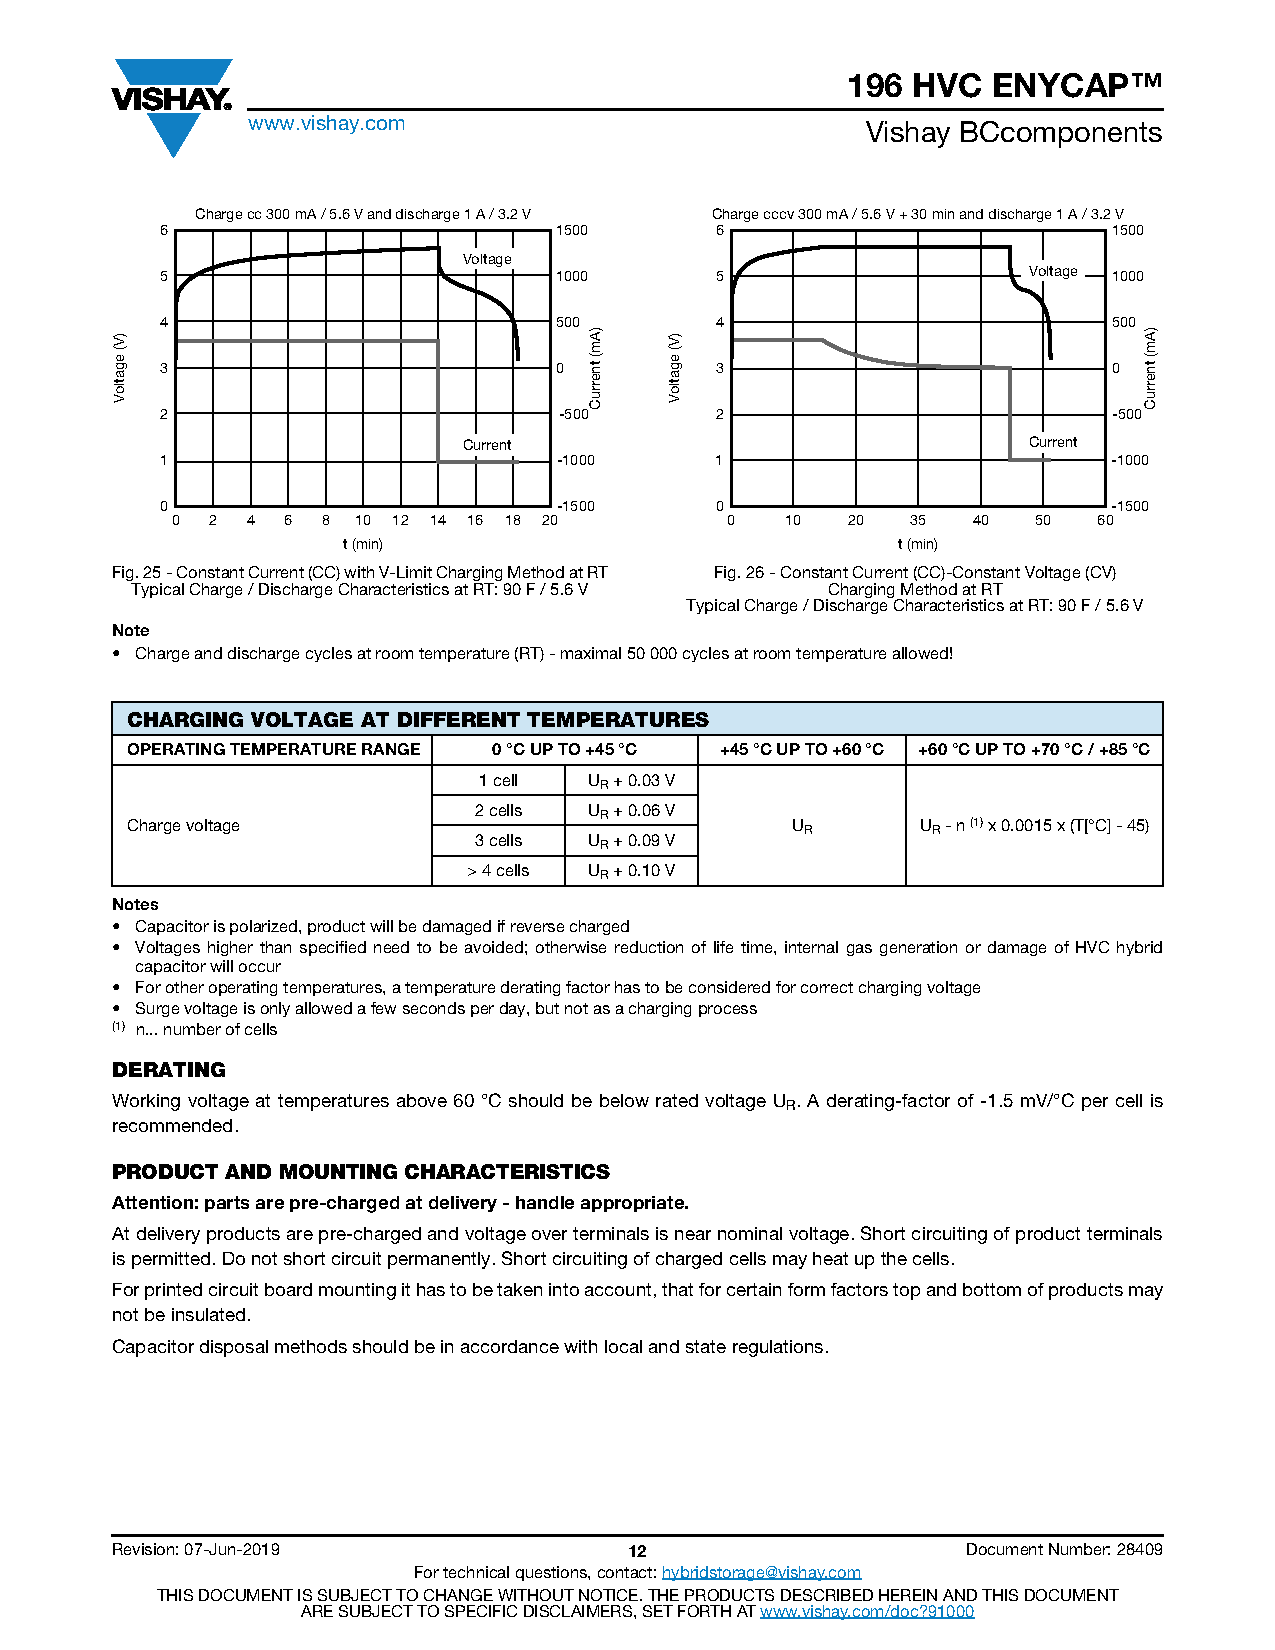
\includegraphics[width=0.6\textwidth]{196hvc-12.pdf}
    \caption[Constant current charge and discharge: \SI{90}{F} / \SI{5.6}{V}]{Constant current charge and discharge: \SI{90}{F} / \SI{5.6}{V}~\cite{Vishay}}
    \label{fig:hvc}
\end{figure}

The all-in-one supercapacitor of \SI{90}{F} is selected because its capacitance is 50\% higher and its cost is lower with not much additional leakage current and space on the board. It thus allows more power consumption (namely processing in the microcontroller) during periods of higher sunlight without saturating the supercapacitor voltage. Based on Figure~\ref{fig:Supercap_voltage_C}, it is expected that the voltage follows the red curve and thus reaches a peak at \SI{3.8}{V}.

Figure~\ref{fig:Supercap_voltage_voltage_split} gives the voltage split for a \SI{90}{F} / \SI{4.2}{V} supercap, which perfectly fits into the PMU and supply specifications.

\begin{figure}[H]
\centering
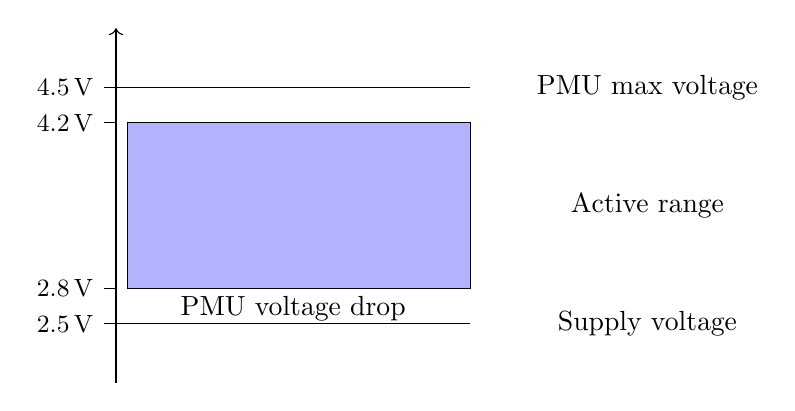
\begin{tikzpicture}[scale=1.5]
% Axes:
\draw[->](0,2)--(0,5);
\draw[](-0.1,4.5)--(0,4.5)node[left,font=\small]{\SI{4.5}{V} \, };
\draw[](-0.1,4.2)--(0,4.2)node[left,font=\small]{\SI{4.2}{V} \, };
\draw[](-0.1,2.8)--(0,2.8)node[left,font=\small]{\SI{2.8}{V} \, };
\draw[](-0.1,2.5)--(0,2.5)node[left,font=\small]{\SI{2.5}{V} \, };
\draw[fill=blue!30] (0.1,2.8) rectangle ++(2.9,1.4);
\draw[](0,4.5)--(3,4.5);
\draw[](0,2.5)--(3,2.5);
\node () [] at (1.5,2.63) {PMU voltage drop};
\node () [] at (4.5,2.5) {Supply voltage};
\node () [] at (4.5,3.5) {Active range};
\node () [] at (4.5,4.5) {PMU max voltage};
\end{tikzpicture}
\caption{Voltage split for a \SI{90}{F} / \SI{4.2}{V} supercap coupled with the AEM10941}
\label{fig:Supercap_voltage_voltage_split}
\end{figure}


\chapter{Final model}

\section{Description}

Figure~\ref{fig:electronics_diagram} presents the electronics diagram of the final model, it summarizes all the blocks previously analyzed and characterized.

\begin{figure}[H]
    \centering
    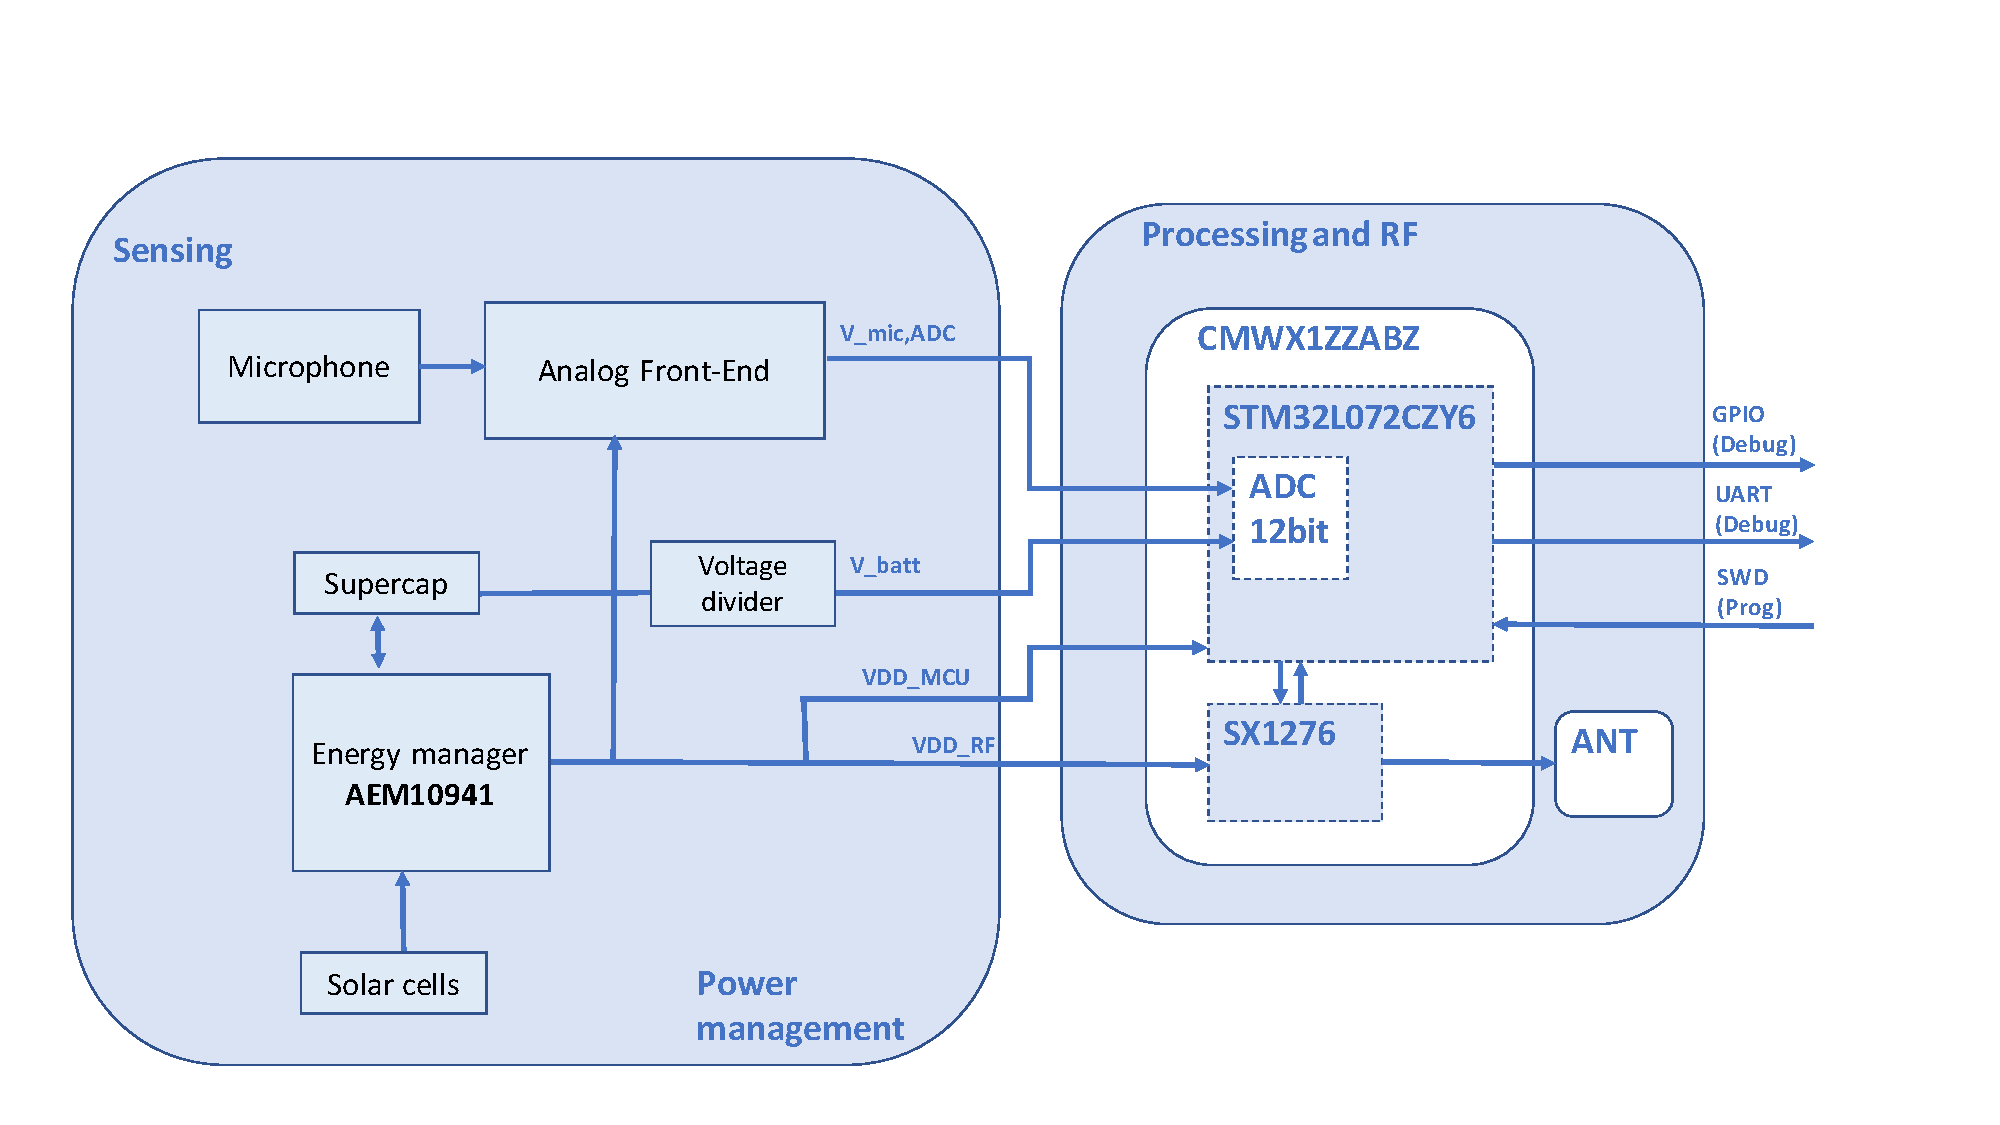
\includegraphics[width=0.8\textwidth]{electronics_diagram.pdf}
    \caption{Electronics diagram of the final model}
    \label{fig:electronics_diagram}
\end{figure}

The final model is a stack of two boards: a board for data processing and radio frequency on top of a board for sensing and power management.

\section{Design}

The design of the final model is given in Figure~\ref{fig:final_model_picture}. One can see the six solar cells, the supercapacitor in blue, the microphone in light gray, as well as five headers for current/voltage measurements. The components are placed such that the solar cells receive the maximum of sunlight.

\begin{figure}[H]
\begin{subfigure}{.5\textwidth}
  \centering
  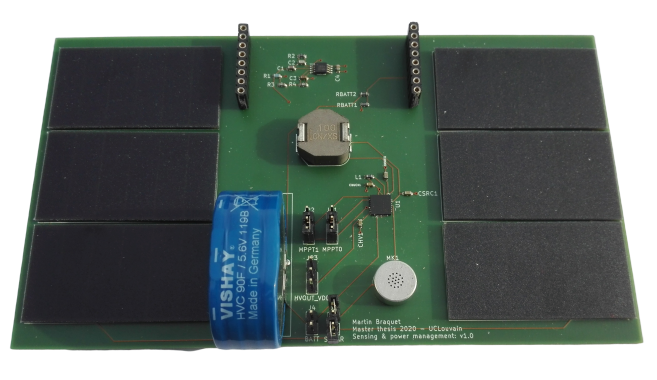
\includegraphics[width=.9\linewidth]{real_PCB.png}  
  \caption{Without MCU/RF board}
\end{subfigure}
\begin{subfigure}{.48\textwidth}
  \centering
  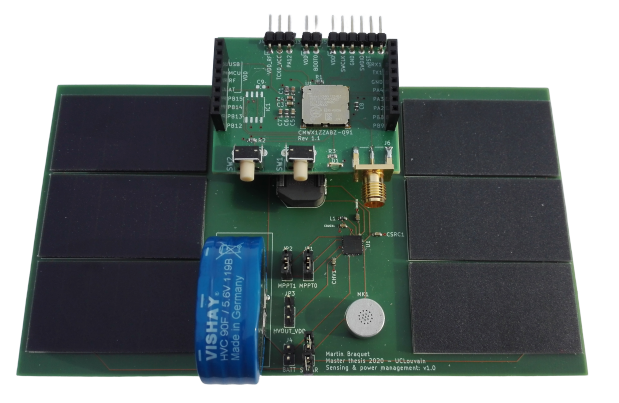
\includegraphics[width=.9\linewidth]{real_PCB_with_MCU.png}  
  \caption{With MCU/RF board}
\end{subfigure}
\caption{Pictures of the final model}
\label{fig:final_model_picture}
\end{figure}

\subsection*{Prototyping}

The PCB schematic and layout are available in Appendix~\ref{appendix:schematic}.

\section{Validation}

This section describes the experimental results obtained with the real device.

\subsection*{Power consumption}

The current consumption measured in the different parts is given in Table~\ref{tab:val_current_cons}. These measurements have been made with a Source Measure Unit: Keithley 2400~\cite{Keithley}.

\begin{table}[H]
\centering
\begin{tabular}{lc}
\toprule
                     & Current [\si{\micro A}]  \\ \midrule
 Supercap leakage    & 95                       \\
 Sensing             & 904                     \\
 PMU                 & 50                       \\
 MCU                 & 470                      \\ \midrule
 Total               & 1645                     \\ \bottomrule
\end{tabular}
\caption{Description of the current consumption in the system}
\label{tab:val_current_cons}
\end{table}

When the supercapacitor is fully disconnected, a leakage current of \SI{95}{\micro A} is noticed, which is indeed below the maximum value of \SI{500}{\micro A} in the datasheet.

In the AFE, the microphone consumes \SI{380}{\micro A}. The op-amp consumes \SI{524}{\micro A}, which is more than expected since it has two channels. One should have chosen an op-amp with only one channel.

As given in the datasheet, the PMU quiescent current is less than \SI{60}{\micro A} (\SI{50}{\micro A}).

The current consumption for a basic code in the MCU (FFT operations without RF and  duty cycle run/deepsleep mode of 10\%) is \SI{470}{\micro A}, corresponding to a run mode consuming \SI{4.7}{mA}. It is approximately the result obtained in the theoretical section.

\subsection*{Solar cells}

Table~\ref{tab:val_current_solar_sel} compares the harvested power from the solar cells in function of the MMP ratio under a fixed interior lighting. The voltage is fixed by the SMU while it measures the current. The highest power is achieved at 70\% of the open-circuit voltage (\SI{4.15}{V}), which is selected in hardware via a header connected to the PMU. For low supercap voltage (below \SI{3.3}{V}), this \SI{2.9}{V} MPPT voltage will not lead to the best PMU efficiency since it exceeds the \SI{2.4}{V} derived in Section~\ref{section:PMU}, but the gain in solar power at this MPP compensates for the loss of efficiency.

\begin{table}[H]
\centering
\begin{tabular}{lccc}
\toprule
  MPPT ratio & Voltage [V] & Current [mA] & Power [mW]  \\ \midrule
 70\%        & 2.9         & 20.2         & 58.6        \\
 75\%        & 3.11        & 17.9         & 55.7        \\
 85\%        & 3.53        & 11.1         & 39.1        \\
 90\%        & 3.73        & 3.5          & 13.1        \\ \bottomrule
\end{tabular}
\caption{Harvested power from the solar cells in function of the MMP ratio}
\label{tab:val_current_solar_sel}
\end{table}


Table~\ref{tab:val_current_harvested} gives the harvested current under different lighting from the solar cells at the MMP voltage (\SI{2.9}{V}). Since the data were taken at noon, they show more harvesting energy than for the theoretical analysis (see Figure~\ref{fig:daily_luminosity}).

\begin{table}[H]
\centering
\begin{tabular}{lc}
\toprule
                     & Current [\si{mA}]  \\ \midrule
 In the shade        & 30                 \\
 Cloudy              & 50                 \\
 Sunny               & 105                \\ \bottomrule
\end{tabular}
\caption{Harvested current under different lighting from the solar cells at the MMP voltage}
\label{tab:val_current_harvested}
\end{table}

\subsection*{Supercapacitor}

Figure~\ref{fig:discharge_supercap_exp} needs to be compared to Figure~\ref{fig:hvc}, it provides the supercapacitor discharge under a constant current of \SI{500}{mA} after being charged to its maximum voltage (\SI{4.2}{V}) and kept at this voltage for 30 minutes (as recommended in the datasheet). It can be noted that the voltage is around \SI{3.1}{V} for the most important part of the operation, which is beneficial since the LDO in the PMU has a low dropout in this case (and thus a good efficiency). Additionally, the supercapacitor is not in operation under \SI{2.5}{V}, which proves that the best type of DC-DC converter for this application is an LDO (and not a buck-boost converter which would allow stepping up the voltage as well). The total energy stored in this \SI{90}{F}/\SI{4.2}{V} supercapacitor is computed as
\[
 E_\te{SC} = \int_0^\infty P_\te{SC}(t) \, \te{d} t = I_\te{discharge} \int_0^\infty V_\te{SC}(t) \, \te{d} t = \SI{851.6}{J}
\]
and is slightly different from the usual equation describing the energy in a capacitor: $E_\te{cap} = C\,V^2/2 = \SI{793.8}{J}$.

\begin{figure}[H]
    \centering
    % This file was created by matlab2tikz.
%
%The latest updates can be retrieved from
%  http://www.mathworks.com/matlabcentral/fileexchange/22022-matlab2tikz-matlab2tikz
%where you can also make suggestions and rate matlab2tikz.
%
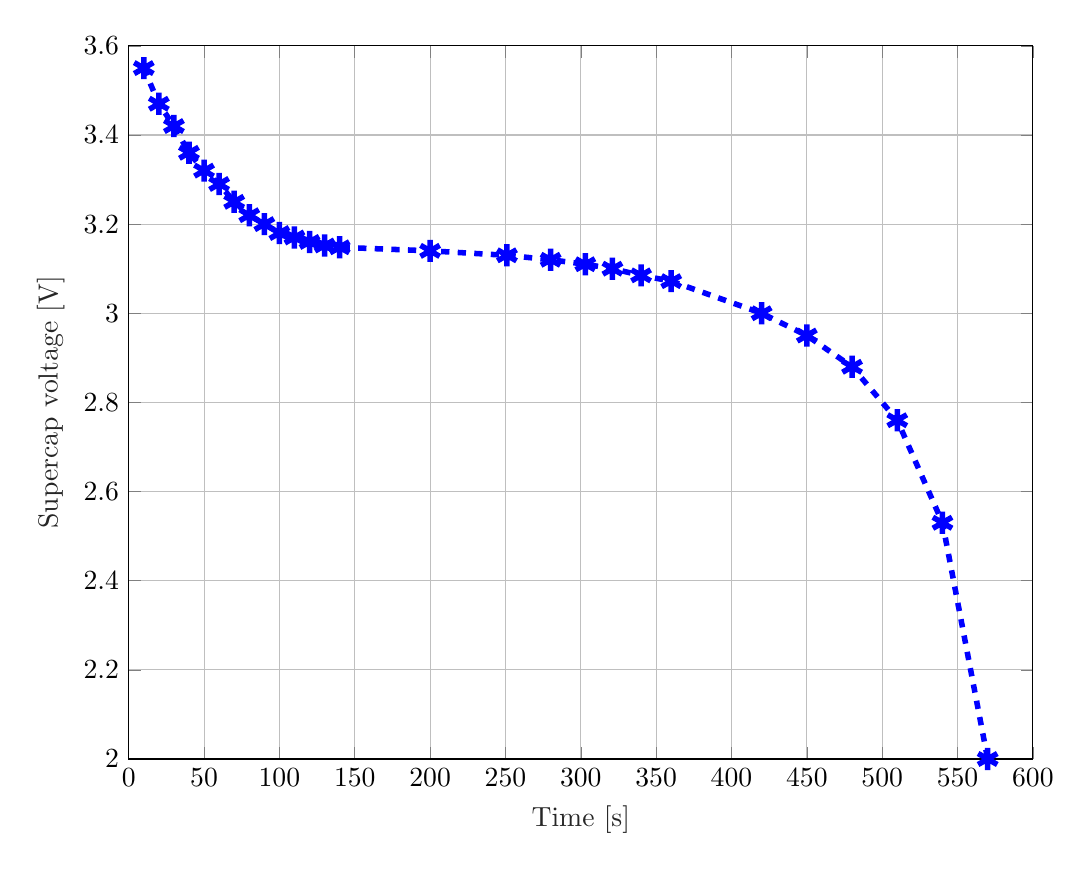
\begin{tikzpicture}

\begin{axis}[%
width=4.521in,
height=3.566in,
at={(0.758in,0.481in)},
scale only axis,
xmin=0,
xmax=600,
xlabel style={font=\color{white!15!black}},
xlabel={Time [s]},
ymin=2,
ymax=3.6,
ylabel style={font=\color{white!15!black}},
ylabel={Supercap voltage [V]},
axis background/.style={fill=white},
xmajorgrids,
ymajorgrids
]
\addplot [color=blue, dashed, line width=2.0pt, mark size=4.0pt, mark=asterisk, mark options={solid, blue}, forget plot]
  table[row sep=crcr]{%
10	3.55\\
20	3.47\\
30	3.42\\
40	3.36\\
50	3.32\\
60	3.29\\
70	3.25\\
80	3.22\\
90	3.2\\
100	3.18\\
110	3.17\\
120	3.16\\
130	3.152\\
140	3.148\\
200	3.14\\
251	3.13\\
280	3.12\\
303	3.11\\
321	3.1\\
340	3.085\\
360	3.072\\
420	3\\
450	2.95\\
480	2.88\\
510	2.76\\
540	2.53\\
570	2\\
};
\end{axis}
\end{tikzpicture}%

    \caption{Supercapacitor discharge under a constant current of \SI{500}{mA}}
    \label{fig:discharge_supercap_exp}
\end{figure}


\subsection*{Sound analysis}

\subsubsection*{Pure sine wave}

To validate the sensing subsystem, a first test is achieved with a pure sine wave at \SI{1}{kHz} generated from a laptop speaker. Figure~\ref{fig:sine_sound} presents the results in the time and frequency domains. This sound is fully detected by the microcontroller, with a sharp peak at \SI{1}{kHz} in the spectral domain. The voltage decrease is probably due to the ADC discharging the node by drawing some current when it samples the signal.

\begin{figure}[H]
\begin{subfigure}{.5\textwidth}
  \centering
  % This file was created by matlab2tikz.
%
%The latest updates can be retrieved from
%  http://www.mathworks.com/matlabcentral/fileexchange/22022-matlab2tikz-matlab2tikz
%where you can also make suggestions and rate matlab2tikz.
%
\definecolor{mycolor1}{rgb}{0.00000,0.44700,0.74100}%
%
\begin{tikzpicture}[scale=0.6]

\begin{axis}[%
width=4.521in,
height=3.566in,
at={(0.758in,0.481in)},
scale only axis,
xmin=0,
xmax=1200,
xlabel style={font=\color{white!15!black}},
xlabel={Samples},
ymin=1800,
ymax=2800,
ylabel style={font=\color{white!15!black}},
ylabel={ADC digitized value},
axis background/.style={fill=white},
xmajorgrids,
ymajorgrids
]
\addplot [color=mycolor1, line width=2.0pt, forget plot]
  table[row sep=crcr]{%
1	2245\\
2	2238\\
3	2273\\
4	2275\\
5	2361\\
6	2430\\
7	2395\\
8	2354\\
9	2347\\
10	2334\\
11	2323\\
12	2325\\
13	2333\\
14	2313\\
15	2306\\
16	2305\\
17	2300\\
18	2316\\
19	2303\\
20	2308\\
21	2311\\
22	2328\\
23	2319\\
24	2352\\
25	2341\\
26	2372\\
27	2370\\
28	2393\\
29	2386\\
30	2427\\
31	2424\\
32	2440\\
33	2463\\
34	2463\\
35	2499\\
36	2498\\
37	2537\\
38	2534\\
39	2566\\
40	2566\\
41	2596\\
42	2590\\
43	2630\\
44	2624\\
45	2644\\
46	2641\\
47	2677\\
48	2670\\
49	2699\\
50	2692\\
51	2701\\
52	2705\\
53	2712\\
54	2730\\
55	2725\\
56	2737\\
57	2740\\
58	2741\\
59	2731\\
60	2739\\
61	2730\\
62	2731\\
63	2730\\
64	2727\\
65	2714\\
66	2722\\
67	2709\\
68	2699\\
69	2694\\
70	2671\\
71	2662\\
72	2657\\
73	2629\\
74	2621\\
75	2591\\
76	2590\\
77	2564\\
78	2552\\
79	2534\\
80	2522\\
81	2489\\
82	2479\\
83	2458\\
84	2442\\
85	2420\\
86	2408\\
87	2386\\
88	2372\\
89	2356\\
90	2339\\
91	2331\\
92	2313\\
93	2300\\
94	2275\\
95	2264\\
96	2254\\
97	2242\\
98	2228\\
99	2223\\
100	2217\\
101	2216\\
102	2206\\
103	2202\\
104	2214\\
105	2199\\
106	2216\\
107	2205\\
108	2229\\
109	2219\\
110	2241\\
111	2237\\
112	2261\\
113	2257\\
114	2283\\
115	2280\\
116	2308\\
117	2308\\
118	2319\\
119	2350\\
120	2347\\
121	2394\\
122	2385\\
123	2431\\
124	2437\\
125	2454\\
126	2447\\
127	2493\\
128	2483\\
129	2514\\
130	2514\\
131	2552\\
132	2546\\
133	2576\\
134	2573\\
135	2591\\
136	2592\\
137	2597\\
138	2606\\
139	2615\\
140	2640\\
141	2634\\
142	2637\\
143	2633\\
144	2655\\
145	2643\\
146	2654\\
147	2649\\
148	2650\\
149	2642\\
150	2643\\
151	2638\\
152	2634\\
153	2626\\
154	2618\\
155	2602\\
156	2607\\
157	2591\\
158	2589\\
159	2565\\
160	2555\\
161	2535\\
162	2526\\
163	2501\\
164	2493\\
165	2461\\
166	2455\\
167	2432\\
168	2418\\
169	2406\\
170	2392\\
171	2357\\
172	2347\\
173	2324\\
174	2309\\
175	2295\\
176	2287\\
177	2272\\
178	2254\\
179	2231\\
180	2207\\
181	2195\\
182	2185\\
183	2174\\
184	2170\\
185	2157\\
186	2158\\
187	2145\\
188	2142\\
189	2143\\
190	2142\\
191	2135\\
192	2138\\
193	2133\\
194	2148\\
195	2141\\
196	2146\\
197	2143\\
198	2171\\
199	2165\\
200	2201\\
201	2193\\
202	2229\\
203	2224\\
204	2228\\
205	2261\\
206	2260\\
207	2295\\
208	2295\\
209	2327\\
210	2323\\
211	2381\\
212	2375\\
213	2400\\
214	2398\\
215	2417\\
216	2413\\
217	2465\\
218	2451\\
219	2488\\
220	2481\\
221	2508\\
222	2501\\
223	2525\\
224	2527\\
225	2542\\
226	2548\\
227	2551\\
228	2569\\
229	2559\\
230	2578\\
231	2574\\
232	2579\\
233	2572\\
234	2578\\
235	2567\\
236	2582\\
237	2571\\
238	2569\\
239	2562\\
240	2561\\
241	2547\\
242	2548\\
243	2537\\
244	2524\\
245	2498\\
246	2492\\
247	2482\\
248	2472\\
249	2445\\
250	2436\\
251	2413\\
252	2402\\
253	2382\\
254	2372\\
255	2342\\
256	2337\\
257	2307\\
258	2295\\
259	2270\\
260	2258\\
261	2237\\
262	2231\\
263	2209\\
264	2192\\
265	2175\\
266	2151\\
267	2142\\
268	2124\\
269	2113\\
270	2105\\
271	2091\\
272	2087\\
273	2077\\
274	2070\\
275	2061\\
276	2071\\
277	2058\\
278	2064\\
279	2056\\
280	2064\\
281	2061\\
282	2068\\
283	2058\\
284	2096\\
285	2084\\
286	2102\\
287	2107\\
288	2108\\
289	2115\\
290	2134\\
291	2166\\
292	2160\\
293	2197\\
294	2188\\
295	2218\\
296	2216\\
297	2252\\
298	2253\\
299	2290\\
300	2283\\
301	2328\\
302	2325\\
303	2366\\
304	2360\\
305	2388\\
306	2389\\
307	2411\\
308	2408\\
309	2423\\
310	2451\\
311	2451\\
312	2477\\
313	2465\\
314	2504\\
315	2491\\
316	2515\\
317	2512\\
318	2514\\
319	2509\\
320	2531\\
321	2519\\
322	2520\\
323	2514\\
324	2509\\
325	2502\\
326	2505\\
327	2493\\
328	2498\\
329	2487\\
330	2474\\
331	2463\\
332	2450\\
333	2443\\
334	2430\\
335	2416\\
336	2404\\
337	2395\\
338	2384\\
339	2358\\
340	2351\\
341	2314\\
342	2309\\
343	2284\\
344	2270\\
345	2247\\
346	2237\\
347	2212\\
348	2201\\
349	2185\\
350	2153\\
351	2145\\
352	2118\\
353	2109\\
354	2090\\
355	2077\\
356	2080\\
357	2061\\
358	2051\\
359	2042\\
360	2031\\
361	2020\\
362	2021\\
363	2013\\
364	2014\\
365	2007\\
366	2020\\
367	2010\\
368	2024\\
369	2019\\
370	2034\\
371	2031\\
372	2043\\
373	2038\\
374	2074\\
375	2069\\
376	2074\\
377	2096\\
378	2093\\
379	2119\\
380	2118\\
381	2155\\
382	2146\\
383	2194\\
384	2192\\
385	2243\\
386	2239\\
387	2266\\
388	2263\\
389	2284\\
390	2289\\
391	2316\\
392	2318\\
393	2351\\
394	2346\\
395	2363\\
396	2370\\
397	2383\\
398	2415\\
399	2410\\
400	2449\\
401	2436\\
402	2460\\
403	2456\\
404	2467\\
405	2458\\
406	2472\\
407	2463\\
408	2472\\
409	2470\\
410	2474\\
411	2462\\
412	2472\\
413	2460\\
414	2451\\
415	2442\\
416	2443\\
417	2427\\
418	2413\\
419	2339\\
420	2320\\
421	2285\\
422	2270\\
423	2268\\
424	2255\\
425	2225\\
426	2219\\
427	2195\\
428	2185\\
429	2162\\
430	2154\\
431	2124\\
432	2116\\
433	2096\\
434	2080\\
435	2070\\
436	2052\\
437	2047\\
438	2016\\
439	2006\\
440	1980\\
441	1973\\
442	1957\\
443	1948\\
444	1925\\
445	1922\\
446	1927\\
447	1914\\
448	1913\\
449	1905\\
450	1901\\
451	1895\\
452	1903\\
453	1891\\
454	1904\\
455	1898\\
456	1906\\
457	1901\\
458	1918\\
459	1912\\
460	1939\\
461	1933\\
462	1941\\
463	1971\\
464	1961\\
465	2005\\
466	1994\\
467	2025\\
468	2020\\
469	2057\\
470	2054\\
471	2094\\
472	2088\\
473	2139\\
474	2144\\
475	2165\\
476	2162\\
477	2197\\
478	2195\\
479	2226\\
480	2222\\
481	2238\\
482	2250\\
483	2274\\
484	2293\\
485	2291\\
486	2312\\
487	2309\\
488	2327\\
489	2323\\
490	2345\\
491	2340\\
492	2354\\
493	2344\\
494	2361\\
495	2356\\
496	2363\\
497	2354\\
498	2353\\
499	2351\\
500	2346\\
501	2338\\
502	2335\\
503	2323\\
504	2317\\
505	2312\\
506	2299\\
507	2297\\
508	2285\\
509	2268\\
510	2261\\
511	2238\\
512	2224\\
513	2199\\
514	2192\\
515	2172\\
516	2161\\
517	2146\\
518	2122\\
519	2113\\
520	2097\\
521	2082\\
522	2056\\
523	2042\\
524	2021\\
525	2007\\
526	1983\\
527	1978\\
528	1960\\
529	1945\\
530	1935\\
531	1919\\
532	1913\\
533	1906\\
534	1896\\
535	1886\\
536	1889\\
537	1883\\
538	1876\\
539	1873\\
540	1873\\
541	1863\\
542	1876\\
543	1873\\
544	1886\\
545	1883\\
546	1901\\
547	1888\\
548	1907\\
549	1929\\
550	1918\\
551	1947\\
552	1943\\
553	1973\\
554	1968\\
555	2016\\
556	2015\\
557	2042\\
558	2044\\
559	2078\\
560	2081\\
561	2126\\
562	2117\\
563	2156\\
564	2156\\
565	2198\\
566	2192\\
567	2209\\
568	2226\\
569	2241\\
570	2264\\
571	2266\\
572	2291\\
573	2292\\
574	2312\\
575	2308\\
576	2341\\
577	2326\\
578	2346\\
579	2339\\
580	2357\\
581	2353\\
582	2351\\
583	2343\\
584	2353\\
585	2341\\
586	2341\\
587	2335\\
588	2337\\
589	2336\\
590	2324\\
591	2320\\
592	2308\\
593	2291\\
594	2286\\
595	2273\\
596	2262\\
597	2242\\
598	2232\\
599	2207\\
600	2194\\
601	2187\\
602	2173\\
603	2146\\
604	2136\\
605	2114\\
606	2096\\
607	2089\\
608	2075\\
609	2060\\
610	2024\\
611	2016\\
612	1991\\
613	1982\\
614	1970\\
615	1961\\
616	1942\\
617	1934\\
618	1915\\
619	1904\\
620	1911\\
621	1892\\
622	1884\\
623	1880\\
624	1878\\
625	1870\\
626	1874\\
627	1873\\
628	1871\\
629	1865\\
630	1877\\
631	1868\\
632	1897\\
633	1885\\
634	1895\\
635	1916\\
636	1910\\
637	1946\\
638	1937\\
639	1981\\
640	1974\\
641	1997\\
642	1995\\
643	2031\\
644	2025\\
645	2068\\
646	2065\\
647	2114\\
648	2113\\
649	2132\\
650	2121\\
651	2164\\
652	2160\\
653	2174\\
654	2186\\
655	2217\\
656	2245\\
657	2240\\
658	2268\\
659	2268\\
660	2293\\
661	2285\\
662	2312\\
663	2305\\
664	2325\\
665	2321\\
666	2340\\
667	2327\\
668	2357\\
669	2345\\
670	2343\\
671	2342\\
672	2345\\
673	2335\\
674	2342\\
675	2329\\
676	2325\\
677	2314\\
678	2307\\
679	2304\\
680	2296\\
681	2278\\
682	2272\\
683	2248\\
684	2238\\
685	2231\\
686	2218\\
687	2191\\
688	2184\\
689	2161\\
690	2152\\
691	2141\\
692	2124\\
693	2118\\
694	2090\\
695	2072\\
696	2043\\
697	2031\\
698	2022\\
699	2006\\
700	1984\\
701	1978\\
702	1958\\
703	1942\\
704	1934\\
705	1922\\
706	1913\\
707	1905\\
708	1898\\
709	1890\\
710	1896\\
711	1882\\
712	1879\\
713	1871\\
714	1869\\
715	1877\\
716	1870\\
717	1886\\
718	1876\\
719	1882\\
720	1896\\
721	1906\\
722	1902\\
723	1931\\
724	1927\\
725	1946\\
726	1944\\
727	1980\\
728	1970\\
729	2013\\
730	2013\\
731	2042\\
732	2040\\
733	2081\\
734	2076\\
735	2130\\
736	2123\\
737	2150\\
738	2132\\
739	2155\\
740	2201\\
741	2192\\
742	2227\\
743	2223\\
744	2259\\
745	2260\\
746	2286\\
747	2281\\
748	2295\\
749	2301\\
750	2317\\
751	2314\\
752	2336\\
753	2329\\
754	2348\\
755	2341\\
756	2358\\
757	2346\\
758	2347\\
759	2346\\
760	2349\\
761	2348\\
762	2332\\
763	2336\\
764	2328\\
765	2319\\
766	2312\\
767	2297\\
768	2290\\
769	2276\\
770	2265\\
771	2253\\
772	2248\\
773	2218\\
774	2207\\
775	2190\\
776	2174\\
777	2153\\
778	2144\\
779	2133\\
780	2104\\
781	2093\\
782	2077\\
783	2062\\
784	2023\\
785	2015\\
786	1995\\
787	1984\\
788	1960\\
789	1949\\
790	1929\\
791	1921\\
792	1912\\
793	1898\\
794	1886\\
795	1875\\
796	1876\\
797	1858\\
798	1854\\
799	1854\\
800	1860\\
801	1850\\
802	1851\\
803	1856\\
804	1851\\
805	1865\\
806	1856\\
807	1874\\
808	1874\\
809	1893\\
810	1883\\
811	1923\\
812	1914\\
813	1945\\
814	1942\\
815	1965\\
816	1966\\
817	2004\\
818	2001\\
819	2036\\
820	2032\\
821	2072\\
822	2068\\
823	2098\\
824	2098\\
825	2125\\
826	2162\\
827	2159\\
828	2188\\
829	2180\\
830	2221\\
831	2218\\
832	2248\\
833	2247\\
834	2274\\
835	2268\\
836	2296\\
837	2290\\
838	2314\\
839	2307\\
840	2335\\
841	2325\\
842	2343\\
843	2335\\
844	2340\\
845	2341\\
846	2336\\
847	2333\\
848	2323\\
849	2325\\
850	2322\\
851	2316\\
852	2303\\
853	2313\\
854	2300\\
855	2279\\
856	2278\\
857	2255\\
858	2245\\
859	2230\\
860	2218\\
861	2200\\
862	2191\\
863	2174\\
864	2164\\
865	2150\\
866	2121\\
867	2116\\
868	2075\\
869	2066\\
870	2048\\
871	2034\\
872	2012\\
873	2000\\
874	1981\\
875	1969\\
876	1959\\
877	1946\\
878	1926\\
879	1920\\
880	1904\\
881	1890\\
882	1886\\
883	1875\\
884	1871\\
885	1858\\
886	1853\\
887	1864\\
888	1853\\
889	1875\\
890	1866\\
891	1859\\
892	1859\\
893	1878\\
894	1871\\
895	1898\\
896	1889\\
897	1917\\
898	1915\\
899	1936\\
900	1929\\
901	1969\\
902	1958\\
903	1990\\
904	1993\\
905	2028\\
906	2019\\
907	2064\\
908	2059\\
909	2075\\
910	2119\\
911	2121\\
912	2144\\
913	2135\\
914	2186\\
915	2187\\
916	2211\\
917	2208\\
918	2230\\
919	2226\\
920	2254\\
921	2255\\
922	2282\\
923	2274\\
924	2312\\
925	2299\\
926	2328\\
927	2322\\
928	2339\\
929	2334\\
930	2336\\
931	2343\\
932	2336\\
933	2338\\
934	2328\\
935	2341\\
936	2326\\
937	2331\\
938	2320\\
939	2316\\
940	2312\\
941	2296\\
942	2282\\
943	2282\\
944	2261\\
945	2246\\
946	2238\\
947	2218\\
948	2200\\
949	2197\\
950	2170\\
951	2172\\
952	2132\\
953	2120\\
954	2098\\
955	2087\\
956	2060\\
957	2054\\
958	2028\\
959	2010\\
960	2000\\
961	1984\\
962	1964\\
963	1955\\
964	1937\\
965	1924\\
966	1905\\
967	1891\\
968	1883\\
969	1874\\
970	1868\\
971	1860\\
972	1846\\
973	1852\\
974	1843\\
975	1837\\
976	1835\\
977	1843\\
978	1835\\
979	1856\\
980	1850\\
981	1869\\
982	1864\\
983	1892\\
984	1885\\
985	1920\\
986	1912\\
987	1938\\
988	1939\\
989	1977\\
990	1968\\
991	2010\\
992	2002\\
993	2040\\
994	2035\\
995	2057\\
996	2062\\
997	2105\\
998	2126\\
999	2126\\
1000	2145\\
1001	2146\\
1002	2187\\
1003	2183\\
1004	2224\\
1005	2216\\
1006	2248\\
1007	2238\\
1008	2272\\
1009	2264\\
1010	2283\\
1011	2290\\
1012	2300\\
1013	2292\\
1014	2325\\
1015	2316\\
1016	2334\\
1017	2326\\
1018	2322\\
1019	2337\\
1020	2324\\
1021	2332\\
1022	2324\\
1023	2319\\
1024	2313\\
};
\end{axis}
\end{tikzpicture}%

  \caption{In the temporal domain}
\end{subfigure}
\begin{subfigure}{.48\textwidth}
  \centering
  % This file was created by matlab2tikz.
%
%The latest updates can be retrieved from
%  http://www.mathworks.com/matlabcentral/fileexchange/22022-matlab2tikz-matlab2tikz
%where you can also make suggestions and rate matlab2tikz.
%
\definecolor{mycolor1}{rgb}{0.00000,0.44700,0.74100}%
%
\begin{tikzpicture}

\begin{axis}[%
width=4.521in,
height=3.566in,
at={(0.758in,0.481in)},
scale only axis,
xmin=0,
xmax=20000,
xlabel style={font=\color{white!15!black}},
xlabel={Frequency [Hz]},
ymin=0,
ymax=300,
ylabel style={font=\color{white!15!black}},
ylabel={Amplitude},
axis background/.style={fill=white},
xmajorgrids,
ymajorgrids
]
\addplot [color=mycolor1, line width=2.0pt, forget plot]
  table[row sep=crcr]{%
0	2128.3359375\\
83.0078125	67.842210726739\\
166.015625	43.2266712849677\\
249.0234375	35.1410328320542\\
332.03125	28.0783858811435\\
415.0390625	20.5731782531802\\
498.046875	22.6921592436701\\
581.0546875	19.2769329145482\\
664.0625	17.9270241517958\\
747.0703125	11.8247277145139\\
830.078125	12.8265612802561\\
913.0859375	12.2769470495786\\
996.09375	9.92430744724606\\
1079.1015625	8.77944835070888\\
1162.109375	8.70213626824916\\
1245.1171875	9.58695568902793\\
1328.125	8.12111782338436\\
1411.1328125	7.22266640150446\\
1494.140625	6.95857045171425\\
1577.1484375	6.69942114633432\\
1660.15625	8.37652816158049\\
1743.1640625	6.0887322403536\\
1826.171875	5.95858813579196\\
1909.1796875	4.67209505751443\\
1992.1875	5.19817258552678\\
2075.1953125	4.13985808197796\\
2158.203125	6.48789547277596\\
2241.2109375	5.17721920377052\\
2324.21875	4.87171183072855\\
2407.2265625	5.20410695552598\\
2490.234375	5.00438612220176\\
2573.2421875	4.51219093309576\\
2656.25	4.30560717474301\\
2739.2578125	4.3895788598457\\
2822.265625	4.22891774946661\\
2905.2734375	3.13387833524413\\
2988.28125	4.3401132420575\\
3071.2890625	3.0876528379905\\
3154.296875	3.9438964217387\\
3237.3046875	3.78424656484571\\
3320.3125	3.74011174888086\\
3403.3203125	3.55444748088883\\
3486.328125	3.29344207091835\\
3569.3359375	3.62672804963234\\
3652.34375	3.27427894236471\\
3735.3515625	2.36414975604451\\
3818.359375	3.54244802214185\\
3901.3671875	4.07340339411593\\
3984.375	2.6323324539685\\
4067.3828125	1.76915633988789\\
4150.390625	2.41530514736726\\
4233.3984375	2.61311594527814\\
4316.40625	2.91861541669355\\
4399.4140625	3.12939456761542\\
4482.421875	3.2000508506785\\
4565.4296875	1.46048206773491\\
4648.4375	2.30620971802665\\
4731.4453125	3.08207995868766\\
4814.453125	3.09604198761111\\
4897.4609375	3.11559010587351\\
4980.46875	2.16603589417242\\
5063.4765625	2.6254887629227\\
5146.484375	2.46123608363838\\
5229.4921875	1.83598960042281\\
5312.5	2.66681856218156\\
5395.5078125	1.84650690699171\\
5478.515625	2.012781971268\\
5561.5234375	2.04728602772633\\
5644.53125	2.31532907844625\\
5727.5390625	1.8317578325718\\
5810.546875	2.01329131789509\\
5893.5546875	2.20581638907399\\
5976.5625	1.34813041794385\\
6059.5703125	1.69212822527577\\
6142.578125	1.43006442156927\\
6225.5859375	1.7191182080846\\
6308.59375	2.00851427921581\\
6391.6015625	1.92426887684002\\
6474.609375	1.17187936338989\\
6557.6171875	0.649967181253985\\
6640.625	1.4178314839534\\
6723.6328125	1.56987621870544\\
6806.640625	1.99537966649444\\
6889.6484375	1.41645331874812\\
6972.65625	1.65567593375088\\
7055.6640625	1.02336220087721\\
7138.671875	1.56187664351268\\
7221.6796875	0.920702024587637\\
7304.6875	1.46549147349398\\
7387.6953125	1.3364128368209\\
7470.703125	1.4616289252489\\
7553.7109375	1.29719407388441\\
7636.71875	0.812910289811976\\
7719.7265625	1.68802928235577\\
7802.734375	0.953307119418493\\
7885.7421875	1.78120776107765\\
7968.75	0.996874932978874\\
8051.7578125	1.78548235168942\\
8134.765625	1.43199848363324\\
8217.7734375	1.65076869504195\\
8300.78125	1.53027402003954\\
8383.7890625	1.16626142491781\\
8466.796875	1.32726396100265\\
8549.8046875	1.43290765373114\\
8632.8125	1.29530738967191\\
8715.8203125	1.46441240321144\\
8798.828125	1.07929600334047\\
8881.8359375	0.225711999295462\\
8964.84375	1.5882641709141\\
9047.8515625	1.4078398665896\\
9130.859375	3.13014006545382\\
9213.8671875	1.43403493998394\\
9296.875	1.62321190621154\\
9379.8828125	1.25204753654333\\
9462.890625	1.71644616727228\\
9545.8984375	1.78684186378408\\
9628.90625	1.14611728696538\\
9711.9140625	1.40252301560894\\
9794.921875	1.24420085894008\\
9877.9296875	1.56769169021725\\
9960.9375	1.6106473254476\\
10043.9453125	1.03243137600143\\
10126.953125	0.749149141069257\\
10209.9609375	0.660322950532874\\
10292.96875	1.04113201516922\\
10375.9765625	1.17920664517998\\
10458.984375	1.14068608808797\\
10541.9921875	1.91243614368859\\
10625	0.802438113804527\\
10708.0078125	1.70069572194777\\
10791.015625	1.61182012758348\\
10874.0234375	1.04029616141284\\
10957.03125	0.821003687992521\\
11040.0390625	1.34674672009063\\
11123.046875	0.598533617422086\\
11206.0546875	1.68943811084158\\
11289.0625	1.29807881138802\\
11372.0703125	0.226967524417908\\
11455.078125	0.754728952177332\\
11538.0859375	0.992757973899637\\
11621.09375	1.19176440005761\\
11704.1015625	1.25000188107284\\
11787.109375	0.933368802264554\\
11870.1171875	1.03886298550443\\
11953.125	1.14563379925969\\
12036.1328125	0.746169099563683\\
12119.140625	1.16157200799395\\
12202.1484375	0.992098991325438\\
12285.15625	1.26880289298637\\
12368.1640625	0.887288372970089\\
12451.171875	0.335542325584249\\
12534.1796875	0.880180256142985\\
12617.1875	1.13692474862921\\
12700.1953125	1.12388063270309\\
12783.203125	1.18746085877247\\
12866.2109375	0.801808822667173\\
12949.21875	0.976665854426988\\
13032.2265625	0.646886261621135\\
13115.234375	0.733200445737445\\
13198.2421875	1.1044088710268\\
13281.25	0.535516709028409\\
13364.2578125	1.54058794900922\\
13447.265625	0.3729562319764\\
13530.2734375	0.861487721945306\\
13613.28125	0.449091555159376\\
13696.2890625	0.961482429803904\\
13779.296875	0.716880821972265\\
13862.3046875	0.883596114834218\\
13945.3125	0.36553162509426\\
14028.3203125	0.440929141735009\\
14111.328125	0.184910346501589\\
14194.3359375	0.732521077268681\\
14277.34375	0.675888204631662\\
14360.3515625	1.15860901244378\\
14443.359375	1.07237066966324\\
14526.3671875	1.05268651740353\\
14609.375	0.956063346959747\\
14692.3828125	0.844360365814239\\
14775.390625	0.669893190730219\\
14858.3984375	1.11163019525222\\
14941.40625	0.981646903719287\\
15024.4140625	0.514278816629192\\
15107.421875	0.472548937357781\\
15190.4296875	0.735428221031668\\
15273.4375	4.96840353617383\\
15356.4453125	1.00531978222947\\
15439.453125	0.796372820973201\\
15522.4609375	0.472548391918433\\
15605.46875	1.34711940130335\\
15688.4765625	0.962009852686858\\
15771.484375	0.396492134041877\\
15854.4921875	0.898235173841601\\
15937.5	0.767114667935244\\
16020.5078125	1.06032871089242\\
16103.515625	0.352662241013577\\
16186.5234375	1.12942895473559\\
16269.53125	0.910942762832002\\
16352.5390625	0.416583118623205\\
16435.546875	0.951013769342689\\
16518.5546875	0.698053238733573\\
16601.5625	0.643903493181703\\
16684.5703125	0.442979053530718\\
16767.578125	0.560892840192026\\
16850.5859375	0.792443524359367\\
16933.59375	0.537125285846975\\
17016.6015625	0.969198179997204\\
17099.609375	0.637008379622523\\
17182.6171875	0.811876920152633\\
17265.625	0.671839198658863\\
17348.6328125	0.681551070491082\\
17431.640625	0.559175913179453\\
17514.6484375	0.484292426969579\\
17597.65625	0.609113135746997\\
17680.6640625	0.570051450250724\\
17763.671875	0.770881760871142\\
17846.6796875	0.421173455988939\\
17929.6875	0.625009302017711\\
18012.6953125	0.519128413834511\\
18095.703125	0.618101841367973\\
18178.7109375	0.882466769759698\\
18261.71875	0.97856795714011\\
18344.7265625	0.589421277737688\\
18427.734375	0.953700930471925\\
18510.7421875	0.671674436767077\\
18593.75	0.873347694971004\\
18676.7578125	0.544072040089146\\
18759.765625	0.941288798827019\\
18842.7734375	0.647957662195275\\
18925.78125	1.31913124801685\\
19008.7890625	0.911065691727178\\
19091.796875	0.586748833184721\\
19174.8046875	0.730587524790587\\
19257.8125	0.651271282899075\\
19340.8203125	0.485193690743176\\
19423.828125	0.722215043074672\\
19506.8359375	0.754270530304172\\
19589.84375	0.512701363379998\\
19672.8515625	1.03279633314651\\
19755.859375	0.509169104288791\\
19838.8671875	0.42245897322876\\
19921.875	0.387038117062265\\
20004.8828125	1.24901308420424\\
20087.890625	1.11327587931833\\
20170.8984375	0.107590810950836\\
20253.90625	0.698545655724869\\
20336.9140625	0.911358176075547\\
20419.921875	0.789835306795305\\
20502.9296875	0.357323459152237\\
20585.9375	0.173724573974268\\
20668.9453125	0.266651201214555\\
20751.953125	0.79998600106104\\
20834.9609375	0.829466461854481\\
20917.96875	0.404292521744769\\
21000.9765625	0.795662381995783\\
21083.984375	0.489858557326236\\
21166.9921875	0.737548292732478\\
21250	0.665330820041922\\
21333.0078125	0.730678940961606\\
21416.015625	0.569772013349292\\
21499.0234375	0.924087864535842\\
21582.03125	0.758429089119857\\
21665.0390625	0.793406664527574\\
21748.046875	0.621893531225214\\
21831.0546875	0.864703952123895\\
21914.0625	0.579738328741195\\
21997.0703125	0.547365273847701\\
22080.078125	0.608969260456766\\
22163.0859375	0.555490226617281\\
22246.09375	0.461080727527846\\
22329.1015625	0.334430841289973\\
22412.109375	0.375446916989116\\
22495.1171875	0.462474993589103\\
22578.125	0.360665514579685\\
22661.1328125	1.26726170808417\\
22744.140625	0.343798199004712\\
22827.1484375	0.688575447261518\\
22910.15625	0.789968945770573\\
22993.1640625	0.59348585818304\\
23076.171875	0.229518289345732\\
23159.1796875	0.715520372366861\\
23242.1875	0.201453378298878\\
23325.1953125	0.341243106076702\\
23408.203125	1.12800260359856\\
23491.2109375	0.275639066690195\\
23574.21875	0.193087830438884\\
23657.2265625	0.173371562699697\\
23740.234375	0.743812612796981\\
23823.2421875	0.450819562421358\\
23906.25	0.218221630713178\\
23989.2578125	0.249619208658358\\
24072.265625	0.63740231034047\\
24155.2734375	1.12052701270658\\
24238.28125	0.723192259213647\\
24321.2890625	0.990804328981597\\
24404.296875	1.132567830196\\
24487.3046875	0.521847057702485\\
24570.3125	0.580419775945423\\
24653.3203125	0.728967446495366\\
24736.328125	0.0903506293777421\\
24819.3359375	1.19735275447141\\
24902.34375	0.375739358704298\\
24985.3515625	0.984624161088004\\
25068.359375	0.894136637584184\\
25151.3671875	0.575580859714332\\
25234.375	0.407547953043359\\
25317.3828125	0.321167113991741\\
25400.390625	0.816972744475538\\
25483.3984375	0.463422779790557\\
25566.40625	0.350226975345866\\
25649.4140625	0.123206150815728\\
25732.421875	0.496707225326272\\
25815.4296875	0.708591515860015\\
25898.4375	0.582199579447231\\
25981.4453125	0.180836002314359\\
26064.453125	0.376765883055695\\
26147.4609375	0.820565355976047\\
26230.46875	0.422224994704853\\
26313.4765625	0.531548636113091\\
26396.484375	0.341328374912774\\
26479.4921875	0.557066199209629\\
26562.5	0.432214812467483\\
26645.5078125	0.345033566446109\\
26728.515625	0.28834013924372\\
26811.5234375	0.431606389708696\\
26894.53125	0.443774637481571\\
26977.5390625	0.338831546967232\\
27060.546875	0.49334407876531\\
27143.5546875	0.776891481051692\\
27226.5625	0.531241792807317\\
27309.5703125	0.273315697761743\\
27392.578125	0.408469290982734\\
27475.5859375	0.474128301645324\\
27558.59375	0.477243130221011\\
27641.6015625	0.301866979865214\\
27724.609375	0.59648749232939\\
27807.6171875	0.312741884625031\\
27890.625	0.79222276976717\\
27973.6328125	0.751246643682023\\
28056.640625	0.687033670180829\\
28139.6484375	0.439320898746392\\
28222.65625	0.15226623812543\\
28305.6640625	0.559638088510252\\
28388.671875	0.213387540072683\\
28471.6796875	0.385365971767129\\
28554.6875	0.130368176954225\\
28637.6953125	0.875760261626185\\
28720.703125	0.26808902565811\\
28803.7109375	0.573299403814094\\
28886.71875	0.222032248848535\\
28969.7265625	0.471752301470816\\
29052.734375	0.242173791171852\\
29135.7421875	0.688683482011336\\
29218.75	0.364894503583449\\
29301.7578125	0.465728962429651\\
29384.765625	0.251970477608043\\
29467.7734375	0.599805847569887\\
29550.78125	0.568666447138829\\
29633.7890625	0.256934433506051\\
29716.796875	0.696775069468806\\
29799.8046875	0.568159258838067\\
29882.8125	0.247290721465127\\
29965.8203125	0.199069239053532\\
30048.828125	0.158630459126749\\
30131.8359375	0.418162822994462\\
30214.84375	0.32483732500411\\
30297.8515625	0.420979157552191\\
30380.859375	0.463610356706572\\
30463.8671875	0.284791262718601\\
30546.875	1.84243609868041\\
30629.8828125	0.374851276247796\\
30712.890625	0.256334470687773\\
30795.8984375	0.37243283720874\\
30878.90625	0.402914721503774\\
30961.9140625	0.362875558258693\\
31044.921875	0.912388025618406\\
31127.9296875	0.203813713805578\\
31210.9375	0.252550987505294\\
31293.9453125	0.137242083112252\\
31376.953125	0.420153889941562\\
31459.9609375	0.486852878241922\\
31542.96875	0.508125761290234\\
31625.9765625	0.409487820298806\\
31708.984375	0.164523852729147\\
31791.9921875	0.775858624167263\\
31875	0.06581952032657\\
31958.0078125	0.381907579337494\\
32041.015625	0.331468287621287\\
32124.0234375	0.543377206739755\\
32207.03125	0.429897941713416\\
32290.0390625	0.449956353447545\\
32373.046875	0.199751287052161\\
32456.0546875	0.509673391275528\\
32539.0625	0.291727651985622\\
32622.0703125	0.200305800664611\\
32705.078125	0.488006898562123\\
32788.0859375	0.305793147403254\\
32871.09375	0.317299498933939\\
32954.1015625	0.691205227799809\\
33037.109375	0.4264781269134\\
33120.1171875	0.325796587305677\\
33203.125	0.480745145605602\\
33286.1328125	0.440461743172229\\
33369.140625	0.169322761893269\\
33452.1484375	0.108282440651551\\
33535.15625	0.274921122922874\\
33618.1640625	0.407312969385812\\
33701.171875	0.23198009445134\\
33784.1796875	0.232400648901344\\
33867.1875	0.298779269175606\\
33950.1953125	0.219039227105241\\
34033.203125	0.421836309485886\\
34116.2109375	0.740720709999405\\
34199.21875	0.138564015533812\\
34282.2265625	0.299588802942305\\
34365.234375	0.316738217871121\\
34448.2421875	0.583958434385688\\
34531.25	0.345642976440829\\
34614.2578125	0.474982505016404\\
34697.265625	0.297689969668058\\
34780.2734375	0.0411921627408949\\
34863.28125	0.487091753090522\\
34946.2890625	0.186078132220839\\
35029.296875	0.121586181771689\\
35112.3046875	0.236020192083321\\
35195.3125	0.141716517487709\\
35278.3203125	0.956520657603773\\
35361.328125	0.382666918416669\\
35444.3359375	0.17511906744597\\
35527.34375	0.128336582460929\\
35610.3515625	0.116940683155626\\
35693.359375	0.368794842062724\\
35776.3671875	0.260060643953008\\
35859.375	0.44684628325336\\
35942.3828125	0.453499457757067\\
36025.390625	0.400401981616164\\
36108.3984375	0.439728141237152\\
36191.40625	0.292730243044189\\
36274.4140625	0.137784437319726\\
36357.421875	0.132356494601599\\
36440.4296875	0.160243381462673\\
36523.4375	0.209013995591848\\
36606.4453125	0.227536393429393\\
36689.453125	0.119127716269357\\
36772.4609375	0.395928600666227\\
36855.46875	0.320702393195875\\
36938.4765625	0.0635441162511979\\
37021.484375	0.057561124508217\\
37104.4921875	0.201683472154557\\
37187.5	0.462106831714081\\
37270.5078125	0.532427787723272\\
37353.515625	0.155318632206935\\
37436.5234375	0.493098904124042\\
37519.53125	0.331388417592571\\
37602.5390625	0.0564502685446747\\
37685.546875	0.45034300578004\\
37768.5546875	0.239735988101195\\
37851.5625	0.21083103726653\\
37934.5703125	0.0779616088686373\\
38017.578125	0.19847920232711\\
38100.5859375	0.287142375120474\\
38183.59375	0.241078409794352\\
38266.6015625	0.104876862064058\\
38349.609375	0.244049893044696\\
38432.6171875	0.247914708990705\\
38515.625	0.465162068487863\\
38598.6328125	0.210250503134549\\
38681.640625	0.433572179283393\\
38764.6484375	0.209296055553533\\
38847.65625	0.301556947043465\\
38930.6640625	0.270251730793659\\
39013.671875	0.251105566555569\\
39096.6796875	0.103951992527629\\
39179.6875	1.09036944660987\\
39262.6953125	0.302751396286248\\
39345.703125	0.434360855228212\\
39428.7109375	0.204155781548904\\
39511.71875	0.409465978867614\\
39594.7265625	0.37448257090641\\
39677.734375	0.536476096768627\\
39760.7421875	0.366684738154703\\
39843.75	0.255573191770855\\
39926.7578125	0.311536356650565\\
40009.765625	0.239234760411324\\
40092.7734375	0.0542498940592216\\
40175.78125	0.261562169368729\\
40258.7890625	0.265086115901932\\
40341.796875	0.254091040892209\\
40424.8046875	0.108081161303631\\
40507.8125	0.281383683216674\\
40590.8203125	0.282200410671597\\
40673.828125	0.0244996397390394\\
40756.8359375	0.160489833386607\\
40839.84375	0.220921532397543\\
40922.8515625	0.315662462759959\\
41005.859375	0.240777568288829\\
41088.8671875	0.253546034847044\\
41171.875	0.238354713753617\\
41254.8828125	0.215560064937222\\
41337.890625	0.206610015175806\\
41420.8984375	0.0575425238690231\\
41503.90625	0.446878010882923\\
41586.9140625	0.29350556694757\\
41669.921875	0.0294537751571111\\
41752.9296875	0.260164649042828\\
41835.9375	0.444770940763443\\
41918.9453125	0.241534255534488\\
42001.953125	0.241557910618914\\
42084.9609375	0.186644870251146\\
42167.96875	0.428235172281701\\
42250.9765625	0.588395704459272\\
42333.984375	0.581310223218155\\
42416.9921875	0.112315886659517\\
42500	0.009765625\\
};
\end{axis}
\end{tikzpicture}%
  \caption{In the frequency domain}
\end{subfigure}
\caption{Analysis of a pure sine wave at \SI{1}{kHz}}
\label{fig:sine_sound}
\end{figure}


\subsection*{Noise}

Figure~\ref{fig:noise_sound} shows a digitized signal under a quiet environment in order to determine the intrinsic noise of the sensing system. The RMS noise value, in terms of LSBs, is given by
\[
 E_\te{RMS} = \sqrt{\frac{1}{N}\sum_n{\big(x[n]-\te{E}[x]\big)^2}} = \SI{23.6}{LSBs}
\]
where $N$ is the number of samples, $x[n]$ is the $n$-th ADC digitized value and $\te{E}[x]$ is the mean of $x$. This value can be compared to the theoretical value, $E_\te{RMS} = \SI{18.7}{LSBs}$ since $V_\te{N,tot,theor} = \SI{11.2}{mV}$ and one LSB is $V_\te{CC} / 2^{12} = \SI{0.6}{mV}$. The excess noise is due to the environmental noise that remains at the microphone input, which is always present except in an anechoic chamber.

\begin{figure}[H]
    \centering
    % This file was created by matlab2tikz.
%
%The latest updates can be retrieved from
%  http://www.mathworks.com/matlabcentral/fileexchange/22022-matlab2tikz-matlab2tikz
%where you can also make suggestions and rate matlab2tikz.
%
\definecolor{mycolor1}{rgb}{0.00000,0.44700,0.74100}%
%
\begin{tikzpicture}[scale=0.8]

\begin{axis}[%
width=4.521in,
height=3.566in,
at={(0.758in,0.481in)},
scale only axis,
xmin=0,
xmax=1000,
xlabel style={font=\color{white!15!black}},
xlabel={Samples},
ymin=2010,
ymax=2100,
ylabel style={font=\color{white!15!black}},
ylabel={ADC digitized value},
axis background/.style={fill=white},
xmajorgrids,
ymajorgrids
]
\addplot [color=mycolor1, line width=2.0pt, forget plot]
  table[row sep=crcr]{%
1	2074\\
2	2073\\
3	2075\\
4	2070\\
5	2058\\
6	2070\\
7	2074\\
8	2070\\
9	2076\\
10	2058\\
11	2056\\
12	2055\\
13	2070\\
14	2070\\
15	2058\\
16	2046\\
17	2047\\
18	2046\\
19	2042\\
20	2050\\
21	2052\\
22	2042\\
23	2043\\
24	2055\\
25	2066\\
26	2062\\
27	2042\\
28	2054\\
29	2050\\
30	2039\\
31	2042\\
32	2039\\
33	2030\\
34	2033\\
35	2043\\
36	2052\\
37	2041\\
38	2030\\
39	2032\\
40	2023\\
41	2037\\
42	2039\\
43	2044\\
44	2028\\
45	2027\\
46	2045\\
47	2058\\
48	2051\\
49	2057\\
50	2050\\
51	2043\\
52	2055\\
53	2053\\
54	2063\\
55	2048\\
56	2048\\
57	2045\\
58	2054\\
59	2061\\
60	2045\\
61	2049\\
62	2040\\
63	2045\\
64	2045\\
65	2053\\
66	2045\\
67	2043\\
68	2040\\
69	2056\\
70	2052\\
71	2059\\
72	2043\\
73	2042\\
74	2049\\
75	2053\\
76	2053\\
77	2035\\
78	2045\\
79	2052\\
80	2064\\
81	2060\\
82	2045\\
83	2053\\
84	2053\\
85	2055\\
86	2049\\
87	2056\\
88	2052\\
89	2038\\
90	2041\\
91	2051\\
92	2053\\
93	2051\\
94	2039\\
95	2041\\
96	2041\\
97	2042\\
98	2046\\
99	2025\\
100	2027\\
101	2035\\
102	2026\\
103	2027\\
104	2038\\
105	2028\\
106	2025\\
107	2034\\
108	2044\\
109	2050\\
110	2053\\
111	2039\\
112	2038\\
113	2036\\
114	2039\\
115	2052\\
116	2030\\
117	2032\\
118	2036\\
119	2032\\
120	2033\\
121	2043\\
122	2031\\
123	2036\\
124	2044\\
125	2048\\
126	2057\\
127	2040\\
128	2039\\
129	2038\\
130	2044\\
131	2042\\
132	2039\\
133	2022\\
134	2022\\
135	2033\\
136	2051\\
137	2048\\
138	2040\\
139	2032\\
140	2049\\
141	2042\\
142	2050\\
143	2055\\
144	2038\\
145	2045\\
146	2040\\
147	2062\\
148	2058\\
149	2064\\
150	2054\\
151	2060\\
152	2062\\
153	2070\\
154	2075\\
155	2059\\
156	2064\\
157	2060\\
158	2057\\
159	2059\\
160	2066\\
161	2054\\
162	2059\\
163	2054\\
164	2058\\
165	2072\\
166	2060\\
167	2059\\
168	2064\\
169	2069\\
170	2078\\
171	2079\\
172	2064\\
173	2074\\
174	2070\\
175	2064\\
176	2066\\
177	2063\\
178	2053\\
179	2052\\
180	2052\\
181	2054\\
182	2059\\
183	2043\\
184	2057\\
185	2052\\
186	2064\\
187	2066\\
188	2052\\
189	2042\\
190	2058\\
191	2061\\
192	2059\\
193	2060\\
194	2044\\
195	2055\\
196	2061\\
197	2059\\
198	2055\\
199	2059\\
200	2044\\
201	2044\\
202	2049\\
203	2053\\
204	2056\\
205	2036\\
206	2037\\
207	2036\\
208	2041\\
209	2049\\
210	2040\\
211	2042\\
212	2039\\
213	2040\\
214	2045\\
215	2056\\
216	2051\\
217	2036\\
218	2042\\
219	2044\\
220	2048\\
221	2042\\
222	2031\\
223	2047\\
224	2044\\
225	2049\\
226	2034\\
227	2020\\
228	2029\\
229	2028\\
230	2028\\
231	2032\\
232	2027\\
233	2022\\
234	2010\\
235	2024\\
236	2031\\
237	2033\\
238	2045\\
239	2029\\
240	2027\\
241	2040\\
242	2048\\
243	2051\\
244	2035\\
245	2032\\
246	2033\\
247	2045\\
248	2045\\
249	2048\\
250	2042\\
251	2041\\
252	2043\\
253	2048\\
254	2051\\
255	2039\\
256	2040\\
257	2042\\
258	2045\\
259	2040\\
260	2044\\
261	2029\\
262	2036\\
263	2037\\
264	2056\\
265	2048\\
266	2057\\
267	2048\\
268	2043\\
269	2050\\
270	2059\\
271	2058\\
272	2046\\
273	2056\\
274	2055\\
275	2056\\
276	2058\\
277	2043\\
278	2045\\
279	2049\\
280	2050\\
281	2053\\
282	2053\\
283	2058\\
284	2040\\
285	2044\\
286	2058\\
287	2056\\
288	2066\\
289	2056\\
290	2054\\
291	2059\\
292	2056\\
293	2056\\
294	2050\\
295	2040\\
296	2041\\
297	2058\\
298	2054\\
299	2057\\
300	2036\\
301	2034\\
302	2034\\
303	2046\\
304	2055\\
305	2049\\
306	2034\\
307	2043\\
308	2047\\
309	2057\\
310	2055\\
311	2041\\
312	2044\\
313	2043\\
314	2065\\
315	2055\\
316	2044\\
317	2044\\
318	2043\\
319	2048\\
320	2044\\
321	2044\\
322	2035\\
323	2038\\
324	2048\\
325	2054\\
326	2056\\
327	2065\\
328	2045\\
329	2048\\
330	2055\\
331	2054\\
332	2060\\
333	2039\\
334	2043\\
335	2039\\
336	2049\\
337	2052\\
338	2057\\
339	2045\\
340	2044\\
341	2050\\
342	2056\\
343	2066\\
344	2048\\
345	2048\\
346	2056\\
347	2066\\
348	2070\\
349	2065\\
350	2052\\
351	2062\\
352	2059\\
353	2071\\
354	2083\\
355	2077\\
356	2062\\
357	2065\\
358	2062\\
359	2074\\
360	2071\\
361	2056\\
362	2067\\
363	2059\\
364	2075\\
365	2074\\
366	2077\\
367	2064\\
368	2064\\
369	2061\\
370	2069\\
371	2071\\
372	2054\\
373	2054\\
374	2057\\
375	2057\\
376	2066\\
377	2073\\
378	2060\\
379	2068\\
380	2064\\
381	2070\\
382	2075\\
383	2065\\
384	2059\\
385	2065\\
386	2074\\
387	2077\\
388	2074\\
389	2063\\
390	2064\\
391	2065\\
392	2059\\
393	2059\\
394	2066\\
395	2048\\
396	2057\\
397	2061\\
398	2066\\
399	2060\\
400	2046\\
401	2052\\
402	2048\\
403	2061\\
404	2048\\
405	2036\\
406	2045\\
407	2040\\
408	2044\\
409	2054\\
410	2053\\
411	2058\\
412	2045\\
413	2056\\
414	2050\\
415	2051\\
416	2056\\
417	2044\\
418	2034\\
419	2035\\
420	2045\\
421	2055\\
422	2039\\
423	2048\\
424	2053\\
425	2054\\
426	2065\\
427	2044\\
428	2030\\
429	2033\\
430	2037\\
431	2040\\
432	2047\\
433	2046\\
434	2041\\
435	2037\\
436	2044\\
437	2044\\
438	2050\\
439	2035\\
440	2045\\
441	2042\\
442	2048\\
443	2044\\
444	2034\\
445	2037\\
446	2037\\
447	2040\\
448	2040\\
449	2042\\
450	2034\\
451	2044\\
452	2041\\
453	2043\\
454	2051\\
455	2063\\
456	2038\\
457	2054\\
458	2050\\
459	2054\\
460	2058\\
461	2036\\
462	2045\\
463	2044\\
464	2041\\
465	2044\\
466	2055\\
467	2039\\
468	2041\\
469	2052\\
470	2051\\
471	2052\\
472	2037\\
473	2037\\
474	2033\\
475	2046\\
476	2051\\
477	2057\\
478	2040\\
479	2047\\
480	2051\\
481	2049\\
482	2054\\
483	2059\\
484	2046\\
485	2040\\
486	2042\\
487	2046\\
488	2042\\
489	2028\\
490	2032\\
491	2037\\
492	2049\\
493	2043\\
494	2052\\
495	2042\\
496	2038\\
497	2036\\
498	2039\\
499	2038\\
500	2040\\
501	2027\\
502	2030\\
503	2028\\
504	2033\\
505	2038\\
506	2026\\
507	2025\\
508	2027\\
509	2039\\
510	2034\\
511	2020\\
512	2032\\
513	2037\\
514	2047\\
515	2048\\
516	2050\\
517	2031\\
518	2033\\
519	2040\\
520	2040\\
521	2052\\
522	2045\\
523	2038\\
524	2046\\
525	2041\\
526	2056\\
527	2056\\
528	2045\\
529	2041\\
530	2050\\
531	2039\\
532	2051\\
533	2034\\
534	2037\\
535	2033\\
536	2042\\
537	2050\\
538	2061\\
539	2052\\
540	2042\\
541	2058\\
542	2058\\
543	2066\\
544	2070\\
545	2058\\
546	2071\\
547	2062\\
548	2073\\
549	2086\\
550	2070\\
551	2065\\
552	2072\\
553	2070\\
554	2069\\
555	2075\\
556	2063\\
557	2057\\
558	2060\\
559	2057\\
560	2070\\
561	2074\\
562	2058\\
563	2054\\
564	2064\\
565	2075\\
566	2082\\
567	2069\\
568	2070\\
569	2076\\
570	2076\\
571	2080\\
572	2081\\
573	2065\\
574	2076\\
575	2063\\
576	2075\\
577	2069\\
578	2062\\
579	2056\\
580	2056\\
581	2078\\
582	2068\\
583	2067\\
584	2054\\
585	2065\\
586	2061\\
587	2063\\
588	2071\\
589	2067\\
590	2052\\
591	2044\\
592	2053\\
593	2067\\
594	2067\\
595	2046\\
596	2053\\
597	2059\\
598	2068\\
599	2066\\
600	2055\\
601	2048\\
602	2059\\
603	2059\\
604	2052\\
605	2054\\
606	2037\\
607	2045\\
608	2055\\
609	2062\\
610	2062\\
611	2066\\
612	2052\\
613	2044\\
614	2058\\
615	2066\\
616	2064\\
617	2046\\
618	2053\\
619	2054\\
620	2057\\
621	2063\\
622	2049\\
623	2045\\
624	2053\\
625	2051\\
626	2068\\
627	2059\\
628	2072\\
629	2056\\
630	2055\\
631	2068\\
632	2069\\
633	2075\\
634	2065\\
635	2070\\
636	2070\\
637	2071\\
638	2072\\
639	2065\\
640	2065\\
641	2062\\
642	2078\\
643	2076\\
644	2088\\
645	2074\\
646	2073\\
647	2074\\
648	2079\\
649	2080\\
650	2081\\
651	2068\\
652	2072\\
653	2093\\
654	2084\\
655	2092\\
656	2071\\
657	2077\\
658	2078\\
659	2080\\
660	2085\\
661	2090\\
662	2071\\
663	2066\\
664	2074\\
665	2072\\
666	2078\\
667	2067\\
668	2070\\
669	2068\\
670	2080\\
671	2074\\
672	2081\\
673	2066\\
674	2056\\
675	2067\\
676	2071\\
677	2077\\
678	2062\\
679	2066\\
680	2067\\
681	2077\\
682	2078\\
683	2080\\
684	2069\\
685	2058\\
686	2068\\
687	2064\\
688	2056\\
689	2062\\
690	2048\\
691	2046\\
692	2042\\
693	2049\\
694	2042\\
695	2029\\
696	2040\\
697	2035\\
698	2043\\
699	2053\\
700	2043\\
701	2028\\
702	2033\\
703	2034\\
704	2052\\
705	2054\\
706	2040\\
707	2042\\
708	2045\\
709	2054\\
710	2043\\
711	2051\\
712	2037\\
713	2037\\
714	2046\\
715	2049\\
716	2049\\
717	2054\\
718	2039\\
719	2048\\
720	2038\\
721	2055\\
722	2055\\
723	2045\\
724	2053\\
725	2048\\
726	2059\\
727	2053\\
728	2042\\
729	2057\\
730	2057\\
731	2060\\
732	2064\\
733	2072\\
734	2059\\
735	2050\\
736	2062\\
737	2068\\
738	2073\\
739	2072\\
740	2059\\
741	2071\\
742	2096\\
743	2080\\
744	2080\\
745	2058\\
746	2057\\
747	2058\\
748	2067\\
749	2076\\
750	2057\\
751	2051\\
752	2054\\
753	2054\\
754	2063\\
755	2070\\
756	2060\\
757	2051\\
758	2056\\
759	2066\\
760	2062\\
761	2072\\
762	2053\\
763	2057\\
764	2056\\
765	2060\\
766	2067\\
767	2056\\
768	2061\\
769	2064\\
770	2066\\
771	2073\\
772	2068\\
773	2052\\
774	2056\\
775	2054\\
776	2061\\
777	2064\\
778	2067\\
779	2054\\
780	2053\\
781	2053\\
782	2063\\
783	2061\\
784	2049\\
785	2052\\
786	2051\\
787	2060\\
788	2060\\
789	2063\\
790	2043\\
791	2043\\
792	2046\\
793	2050\\
794	2051\\
795	2039\\
796	2040\\
797	2038\\
798	2042\\
799	2045\\
800	2045\\
801	2026\\
802	2033\\
803	2029\\
804	2040\\
805	2048\\
806	2048\\
807	2030\\
808	2034\\
809	2028\\
810	2046\\
811	2051\\
812	2041\\
813	2058\\
814	2050\\
815	2052\\
816	2057\\
817	2058\\
818	2041\\
819	2050\\
820	2058\\
821	2069\\
822	2070\\
823	2079\\
824	2068\\
825	2062\\
826	2066\\
827	2073\\
828	2069\\
829	2051\\
830	2059\\
831	2080\\
832	2072\\
833	2069\\
834	2060\\
835	2056\\
836	2055\\
837	2055\\
838	2061\\
839	2064\\
840	2056\\
841	2056\\
842	2060\\
843	2068\\
844	2059\\
845	2059\\
846	2048\\
847	2050\\
848	2056\\
849	2058\\
850	2059\\
851	2042\\
852	2042\\
853	2043\\
854	2049\\
855	2058\\
856	2041\\
857	2050\\
858	2048\\
859	2060\\
860	2056\\
861	2051\\
862	2058\\
863	2044\\
864	2045\\
865	2052\\
866	2060\\
867	2064\\
868	2056\\
869	2053\\
870	2061\\
871	2062\\
872	2057\\
873	2042\\
874	2047\\
875	2052\\
876	2054\\
877	2057\\
878	2066\\
879	2051\\
880	2044\\
881	2045\\
882	2054\\
883	2061\\
884	2071\\
885	2051\\
886	2052\\
887	2053\\
888	2062\\
889	2065\\
890	2052\\
891	2052\\
892	2056\\
893	2068\\
894	2062\\
895	2066\\
896	2057\\
897	2043\\
898	2058\\
899	2059\\
900	2069\\
901	2058\\
902	2065\\
903	2056\\
904	2069\\
905	2058\\
906	2069\\
907	2052\\
908	2049\\
909	2056\\
910	2064\\
};
\end{axis}
\end{tikzpicture}%

    \caption{Noise at the ADC input}
    \label{fig:noise_sound}
\end{figure}


%\subsection*{...}

%\textcolor{green}{ Current consumption over a whole period with/without Tim's board (material: SMU for 2-3 days)​}

    
\subsection*{Requirements review}

Finally, one will review the requirements stated at the beginning of this work (see Section~\ref{section:requirements}). The requirements related to bird classification will be discussed in the next chapter.

\subsubsection*{Lifetime}

The lifetime is limited by the supercapacitor, which is expected to work about \SI{11200}{h} at \SI{60}{\degree C} according to the datasheet~\cite{Vishay}.   The 10-degrees-rule for electrolytic capacitors can be used to estimate supercapacitor lifetimes. This rule employs the Arrhenius equation, and states that for every \SI{10}{\degree C} reduction in operating temperature, the estimated life doubles. The expected lifetime $L$ at \SI{20}{\degree C} is thus given by
\[
 L = L_0 \, 2^{\frac{T_0-T}{\SI{10}{\degree C}}} = \SI{179200}{h}
\]
which corresponds to 20.5 years. It can even be increased above 20 years with additional equalization methods~\cite{4494753}. As required, the sensor is working fully autonomously (day and night) for more than 15 years.

\subsubsection*{Volume and cost}

One first confirms that the total volume is inside the constraint (\SI{200 x 200 x 50}{mm}): \SI{143 x 82 x 25}{mm}.

The overall cost, including the PCB, is 74.28 euros. The most important costs are the solar cells (30.4 euros), the supercapacitor (17.5 euros) and the PCB (20 euros).  In order to stay below the limit of 15 euros, both the solar cells and supercap need to have a smaller size by reducing the power consumption. Indeed, typical ultra-low-power sensors have a power consumption in the order of the \si{\micro W}~\cite{DEKIMPE20198}. This constraint implies further concessions on the audio processing period over a day. Particularly when the reduced solar cells are strongly limited by the sun illuminance (i.e. in winter), one has to allow the sensor to have a shorter processing period (which fortunately has not much impact since birds are less active in this season). In a massive development, buying in bulk will further help decrease overall costs.


\subsubsection*{Sound detection}

Determining the detection distance is probably the most difficult requirement to precisely characterize. It can be based on real-time songs but birds are singing intermittently and with different sound amplitudes. It can also be characterized by a speaker emitting bird songs, but the sound pressure cannot either be known without a sound level meter. Still, the device has been able to detect pure sine waves with speakers at reasonable distance, as well as bird songs as depicted in the next chapter.

    
\chapter{Inference algorithm}

This chapter will present different algorithms aiming to discriminate bird species based on the microphone signal. This temporal signal is often transformed into its dual domain: the spectral (or frequency) domain. Representing a signal in the spectral domain is done through the Fourier transform, which is in fact a fast Fourier transform (FFT) for digitized data (such as data stored in a microcontroller).

The requirements in Section~\ref{section:requirements} state that the sensor has to discriminate among four very common birds in Belgian forests. These species are the pigeon, blackbird, great tit, and blue tit. The remaining of the section will demonstrate the ability of the sensor node to find the correct species with sufficient precision.

\section{Peak frequency extraction}

The first algorithm will process bird songs based on the frequency at which the signal has the most power. Because the FFT size is limited by computation time, it is not possible to record and process sound over an entire bird song duration (typically \SI{2}{s}). On the other hand, one cannot decrease the sampling frequency below \SI{20}{kHz} in order to detect useful frequencies below \SI{10}{kHz}\footnote{The Nyquist–Shannon sampling theorem states that, to avoid loss of information during a sampling process, a sampling frequency larger than twice the maximum frequency contained in the signal is required.}, which would give \SI{40000}{} samples during a typical song duration. It is thus required to spread the sampling duration over multiple time windows. For example, Figure~\ref{fig:peak_frequency} shows the peak frequency\footnote{That is, there is only one frequency associated with each time sample.} for each time window (\SI{32}{ms} whose \SI{6.4}{ms} to retrieve 128 samples at \SI{20}{kHz}) of a great tit song. One can roughly see two sounds spaced by \SI{4}{ms} and oscillating between \SI{3}{kHz} and \SI{4.5}{kHz}. Based on the graph, it is thus possible to discriminate visually between species with substantially different frequency profiles, but formalizing further embedded processing to extract meaningful information from this peak frequency graph is less trivial.

Although this algorithm shows good visual results, this kind of algorithm misses important information for different reasons.

First, most bird songs present several high amplitudes for different frequencies at the same time, these secondary frequencies are never detected. This means that several bird songs with the same peak frequency but different secondary frequencies are never discriminated.

Second, several birds present different frequency profiles during their song, that is to say the FFT is varying with time (e.g. \SI{3}{kHz} and \SI{4.5}{kHz} for the song presented in Figure~\ref{fig:peak_frequency}). Thereby, characterizing birds based on one FFT over a short period of time misses non-harmonious (or non-periodic) bird songs and cannot discriminate two birds with the same frequency peak in the beginning of their song, for example.

\begin{figure}[H]
    \centering
    % This file was created by matlab2tikz.
%
%The latest updates can be retrieved from
%  http://www.mathworks.com/matlabcentral/fileexchange/22022-matlab2tikz-matlab2tikz
%where you can also make suggestions and rate matlab2tikz.
%
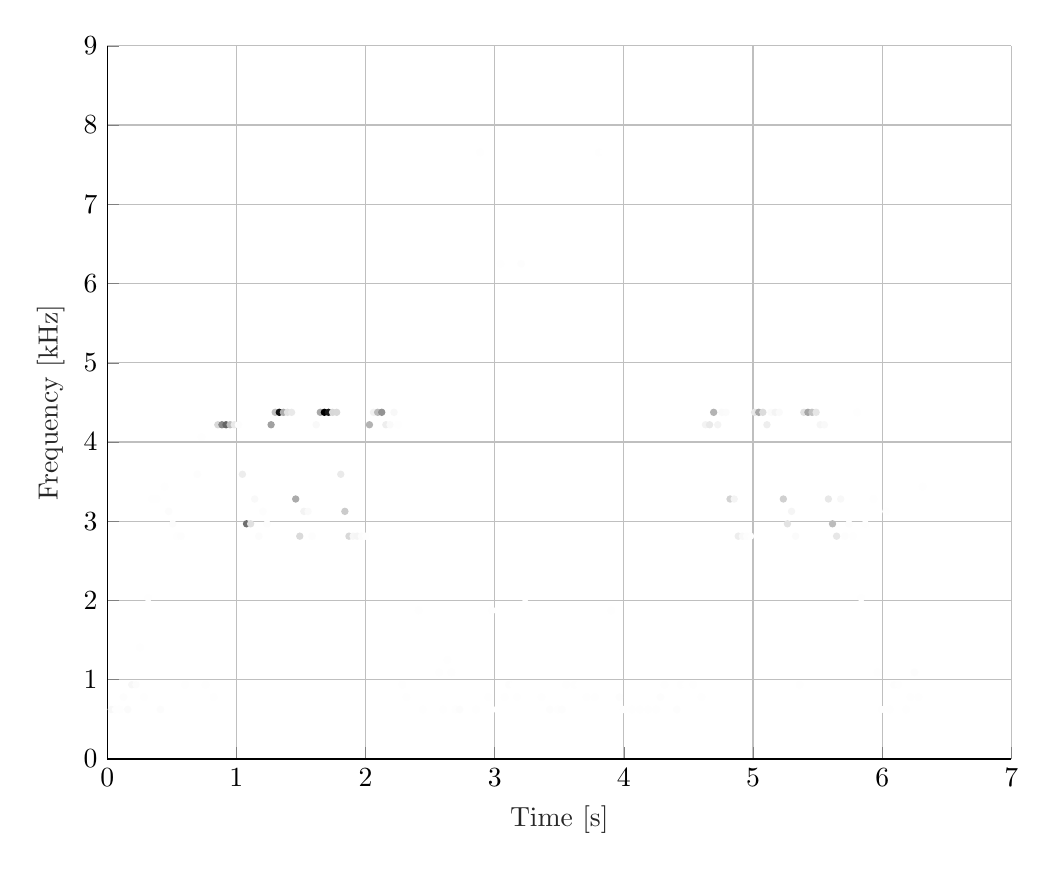
\begin{tikzpicture}

\begin{axis}[%
width=4.521in,
height=3.566in,
at={(0.758in,0.481in)},
scale only axis,
colormap={mymap}{[1pt] rgb(0pt)=(1,1,1); rgb(63pt)=(0,0,0)},
xmin=0,
xmax=7,
xlabel style={font=\color{white!15!black}},
xlabel={Time [s]},
ymin=0,
ymax=9,
ylabel style={font=\color{white!15!black}},
ylabel={Frequency [kHz]},
axis background/.style={fill=white},
axis x line*=bottom,
axis y line*=left,
xmajorgrids,
ymajorgrids
]
\addplot[scatter, only marks, mark=*, mark size=1.1180pt, scatter src=explicit, scatter/use mapped color={mark options={}, draw=mapped color, fill=mapped color}] table[row sep=crcr, meta=color]{%
x	y	color\\
0.031725	0.625	1586\\
0.06345	0.625	494\\
0.095175	0.625	427\\
0.1269	0.781	628\\
0.158625	0.625	944\\
0.19035	0.937	1843\\
0.222075	0.937	882\\
0.2538	1.406	327\\
0.285525	0.781	335\\
0.31725	2.031	313\\
0.348975	3.281	470\\
0.3807	3.281	405\\
0.412425	0.625	757\\
0.44415	3.437	463\\
0.475875	3.125	899\\
0.5076	2.968	873\\
0.539325	2.812	437\\
0.57105	2.812	563\\
0.602775	0.937	450\\
0.6345	3.593	280\\
0.666225	7.656	259\\
0.69795	3.593	559\\
0.729675	4.062	330\\
0.7614	0.937	344\\
0.793125	3.906	237\\
0.82485	0.781	498\\
0.856575	4.218	8327\\
0.8883	4.218	24952\\
0.920025	4.218	32364\\
0.95175	4.218	13677\\
0.983475	4.218	4541\\
1.0152	4.218	546\\
1.046925	3.593	3953\\
1.07865	2.968	30314\\
1.110375	2.968	6461\\
1.1421	3.281	1466\\
1.173825	2.812	854\\
1.20555	3.125	705\\
1.237275	2.968	514\\
1.269	4.218	19951\\
1.300725	4.375	13212\\
1.33245	4.375	49445\\
1.364175	4.375	17530\\
1.3959	4.375	6283\\
1.427625	4.375	4706\\
1.45935	3.281	17800\\
1.491075	2.812	7866\\
1.5228	3.125	2659\\
1.554525	3.125	1194\\
1.58625	2.812	608\\
1.617975	4.218	1354\\
1.6497	4.375	18160\\
1.681425	4.375	53599\\
1.71315	4.375	48352\\
1.744875	4.375	8299\\
1.7766	4.375	8065\\
1.808325	3.593	4677\\
1.84005	3.125	10982\\
1.871775	2.812	8278\\
1.9035	2.812	1974\\
1.935225	2.812	2369\\
1.96695	2.812	785\\
1.998675	2.812	448\\
2.0304	4.218	16101\\
2.062125	4.375	2872\\
2.09385	4.375	14471\\
2.125575	4.375	22884\\
2.1573	4.218	3807\\
2.189025	4.218	1327\\
2.22075	4.375	1761\\
2.252475	4.218	401\\
2.2842	0.937	397\\
2.315925	0.781	323\\
2.34765	4.375	300\\
2.379375	7.5	241\\
2.4111	1.875	439\\
2.442825	0.625	316\\
2.47455	1.562	261\\
2.506275	7.656	271\\
2.538	0.937	299\\
2.569725	1.093	373\\
2.60145	0.625	366\\
2.633175	1.25	414\\
2.6649	1.093	317\\
2.696625	0.625	378\\
2.72835	0.625	773\\
2.760075	7.5	272\\
2.7918	0.781	290\\
2.823525	7.656	271\\
2.85525	0.625	475\\
2.886975	7.656	319\\
2.9187	1.25	268\\
2.950425	0.781	363\\
2.98215	1.875	349\\
3.013875	0.625	255\\
3.0456	6.25	368\\
3.077325	0.781	316\\
3.10905	0.937	518\\
3.140775	0.937	259\\
3.1725	0.781	439\\
3.204225	6.25	659\\
3.23595	2.031	240\\
3.267675	7.656	298\\
3.2994	7.656	292\\
3.331125	0.625	244\\
3.36285	0.781	445\\
3.394575	7.656	197\\
3.4263	0.625	709\\
3.458025	1.093	256\\
3.48975	0.625	384\\
3.521475	0.625	647\\
3.5532	0.937	404\\
3.584925	1.875	266\\
3.61665	0.937	325\\
3.648375	0.937	253\\
3.6801	7.656	286\\
3.711825	0.781	435\\
3.74355	0.625	261\\
3.775275	0.781	372\\
3.807	7.656	329\\
3.838725	7.656	279\\
3.87045	0.937	273\\
3.902175	1.875	399\\
3.9339	7.656	293\\
3.965625	0.781	551\\
3.99735	0.625	326\\
4.029075	1.25	239\\
4.0608	0.625	402\\
4.092525	7.656	272\\
4.12425	0.625	438\\
4.155975	0.937	232\\
4.1877	0.625	379\\
4.219425	0.781	235\\
4.25115	0.625	381\\
4.282875	0.781	527\\
4.3146	0.937	428\\
4.346325	7.656	270\\
4.37805	1.093	297\\
4.409775	0.625	532\\
4.4415	0.937	325\\
4.473225	0.937	247\\
4.50495	3.75	223\\
4.536675	0.937	363\\
4.5684	7.656	269\\
4.600125	0.781	350\\
4.63185	4.218	2749\\
4.663575	4.218	4781\\
4.6953	4.375	16113\\
4.727025	4.218	2418\\
4.75875	4.375	1161\\
4.790475	4.375	1036\\
4.8222	3.281	9511\\
4.853925	3.281	2412\\
4.88565	2.812	4027\\
4.917375	2.812	1351\\
4.9491	2.812	525\\
4.980825	2.812	328\\
5.01255	4.375	5245\\
5.044275	4.375	18037\\
5.076	4.375	7621\\
5.107725	4.218	3722\\
5.13945	4.375	1051\\
5.171175	4.375	2505\\
5.2029	4.375	1155\\
5.234625	3.281	10126\\
5.26635	2.968	6139\\
5.298075	3.125	2327\\
5.3298	2.812	1122\\
5.361525	0.937	430\\
5.39325	4.375	6559\\
5.424975	4.375	19120\\
5.4567	4.375	12688\\
5.488425	4.375	5471\\
5.52015	4.218	2098\\
5.551875	4.218	1394\\
5.5836	3.281	4962\\
5.615325	2.968	14286\\
5.64705	2.812	5143\\
5.678775	3.281	1669\\
5.7105	2.812	634\\
5.742225	2.968	511\\
5.77395	2.812	445\\
5.805675	4.375	424\\
5.8374	2.031	339\\
5.869125	2.968	360\\
5.90085	3.437	268\\
5.932575	3.281	316\\
5.9643	1.093	331\\
5.996025	0.625	450\\
6.02775	3.125	348\\
6.059475	0.625	462\\
6.0912	0.937	668\\
6.122925	0.937	363\\
6.15465	7.656	244\\
6.186375	0.625	342\\
6.2181	0.781	481\\
6.249825	1.093	562\\
6.28155	0.781	436\\
6.313275	3.437	307\\
6.345	7.656	301\\
};
\end{axis}
\end{tikzpicture}%
    \caption{Peak frequencies associated with a great tit song}
    \label{fig:peak_frequency}
\end{figure}


\section{Spectogram decomposition}

From the previous remarks, it is more convenient to represent the signal with a spectrogram: the visual representation of the spectrum of frequencies of a signal as it varies with time. Creating a spectrogram using the FFT is a digital process. Digitally sampled data, in the time domain, are broken up into chunks, which usually overlap, and Fourier transformed to calculate the magnitude of the frequency spectrum for each chunk. Each chunk then corresponds to a vertical line in the image, which provides the magnitude versus frequency for a specific moment.

A smaller (shorter) window will produce more accurate results in timing, at the expense of precision of frequency representation.
This leads to the consideration of trade-offs between time
and frequency resolution in audition: the bandwidth can only be narrowed (i.e. the frequency resolution increased) if the temporal resolution is decreased, because narrower filters have longer time constants.
In the design of linear filters, the uncertainty principle fixes a
limit on the resolution that can be attained (the Gabor limit\footnote{It is nothing else than the Heisenberg's uncertainty principle applied in the context of signal processing to time and frequency (2 dual physical quantities).}),
giving a lower bound for the product of the variance in time
and the variance in frequency for a single linear filter~\cite{Stowell}.

Some birds have several typical songs. For example, Figure~\ref{fig:blue_tit} presents the spectrogram for two common songs of the blue tit. As human perception of sound intensity is logarithmic~\cite{Psychoacoustics}, the graphs are given in the form of log scale.

\begin{figure}[H]
\begin{subfigure}{.48\textwidth}
  \centering
  % This file was created by matlab2tikz.
%
%The latest updates can be retrieved from
%  http://www.mathworks.com/matlabcentral/fileexchange/22022-matlab2tikz-matlab2tikz
%where you can also make suggestions and rate matlab2tikz.
%
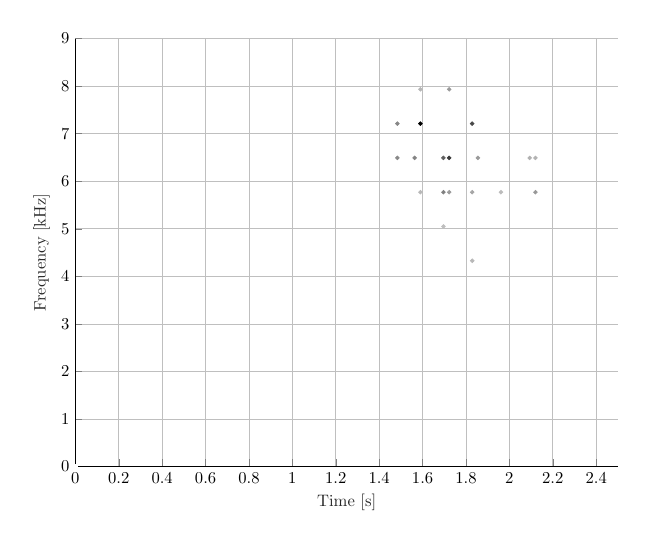
\begin{tikzpicture}[scale=0.6]

\begin{axis}[%
width=4.521in,
height=3.566in,
at={(0.758in,0.481in)},
scale only axis,
colormap={mymap}{[1pt] rgb(0pt)=(1,1,1); rgb(63pt)=(0,0,0)},
xmin=0,
xmax=2.5,
xlabel style={font=\color{white!15!black}},
xlabel={Time [s]},
ymin=0,
ymax=9,
ylabel style={font=\color{white!15!black}},
ylabel={Frequency [kHz]},
axis background/.style={fill=white},
axis x line*=bottom,
axis y line*=left,
xmajorgrids,
ymajorgrids
]
\addplot[scatter, only marks, mark=*, mark size=1.1180pt, scatter src=explicit, scatter/use mapped color={mark options={}, draw=mapped color, fill=mapped color}] table[row sep=crcr, meta=color]{%
x	y	color\\
1.484	6.49014084507042	27612\\
1.484	7.2112676056338	28185\\
1.5635	6.49014084507042	28861\\
1.59	5.76901408450704	16435\\
1.59	7.2112676056338	59874\\
1.59	7.93239436619718	16988\\
1.696	5.04788732394366	15028\\
1.696	5.76901408450704	29869\\
1.696	6.49014084507042	37225\\
1.7225	5.76901408450704	23385\\
1.7225	6.49014084507042	46211\\
1.7225	7.93239436619718	23776\\
1.8285	4.32676056338028	16566\\
1.8285	5.76901408450704	21009\\
1.8285	7.2112676056338	42992\\
1.855	6.49014084507042	23523\\
1.961	5.76901408450704	15761\\
2.0935	6.49014084507042	18271\\
2.12	5.76901408450704	24123\\
2.12	6.49014084507042	17742\\
0	0	0\\
0	0	0\\
0	0	0\\
0	0	0\\
0	0	0\\
0	0	0\\
0	0	0\\
0	0	0\\
0	0	0\\
0	0	0\\
0	0	0\\
0	0	0\\
0	0	0\\
0	0	0\\
0	0	0\\
0	0	0\\
0	0	0\\
0	0	0\\
0	0	0\\
0	0	0\\
0	0	0\\
0	0	0\\
0	0	0\\
0	0	0\\
0	0	0\\
0	0	0\\
0	0	0\\
0	0	0\\
0	0	0\\
0	0	0\\
0	0	0\\
0	0	0\\
0	0	0\\
0	0	0\\
0	0	0\\
0	0	0\\
0	0	0\\
0	0	0\\
0	0	0\\
0	0	0\\
0	0	0\\
0	0	0\\
0	0	0\\
0	0	0\\
0	0	0\\
0	0	0\\
0	0	0\\
0	0	0\\
0	0	0\\
0	0	0\\
0	0	0\\
0	0	0\\
0	0	0\\
0	0	0\\
0	0	0\\
0	0	0\\
0	0	0\\
0	0	0\\
0	0	0\\
0	0	0\\
0	0	0\\
0	0	0\\
0	0	0\\
0	0	0\\
0	0	0\\
0	0	0\\
0	0	0\\
0	0	0\\
0	0	0\\
0	0	0\\
0	0	0\\
0	0	0\\
0	0	0\\
0	0	0\\
0	0	0\\
0	0	0\\
0	0	0\\
0	0	0\\
0	0	0\\
0	0	0\\
0	0	0\\
0	0	0\\
0	0	0\\
0	0	0\\
0	0	0\\
0	0	0\\
0	0	0\\
0	0	0\\
0	0	0\\
0	0	0\\
0	0	0\\
0	0	0\\
0	0	0\\
0	0	0\\
0	0	0\\
0	0	0\\
0	0	0\\
0	0	0\\
0	0	0\\
0	0	0\\
0	0	0\\
0	0	0\\
0	0	0\\
0	0	0\\
0	0	0\\
0	0	0\\
0	0	0\\
0	0	0\\
0	0	0\\
0	0	0\\
0	0	0\\
0	0	0\\
0	0	0\\
0	0	0\\
0	0	0\\
0	0	0\\
0	0	0\\
0	0	0\\
0	0	0\\
0	0	0\\
0	0	0\\
0	0	0\\
0	0	0\\
0	0	0\\
0	0	0\\
0	0	0\\
0	0	0\\
0	0	0\\
0	0	0\\
0	0	0\\
0	0	0\\
0	0	0\\
0	0	0\\
0	0	0\\
0	0	0\\
0	0	0\\
0	0	0\\
0	0	0\\
0	0	0\\
0	0	0\\
0	0	0\\
0	0	0\\
0	0	0\\
0	0	0\\
0	0	0\\
0	0	0\\
0	0	0\\
0	0	0\\
0	0	0\\
0	0	0\\
0	0	0\\
0	0	0\\
0	0	0\\
0	0	0\\
0	0	0\\
0	0	0\\
0	0	0\\
0	0	0\\
0	0	0\\
0	0	0\\
0	0	0\\
0	0	0\\
0	0	0\\
0	0	0\\
0	0	0\\
0	0	0\\
0	0	0\\
0	0	0\\
0	0	0\\
0	0	0\\
0	0	0\\
0	0	0\\
0	0	0\\
0	0	0\\
0	0	0\\
0	0	0\\
0	0	0\\
0	0	0\\
0	0	0\\
0	0	0\\
};
\end{axis}
\end{tikzpicture}%

  \caption{Bird chirp}
\end{subfigure}
\begin{subfigure}{.48\textwidth}
  \centering
  % This file was created by matlab2tikz.
%
%The latest updates can be retrieved from
%  http://www.mathworks.com/matlabcentral/fileexchange/22022-matlab2tikz-matlab2tikz
%where you can also make suggestions and rate matlab2tikz.
%
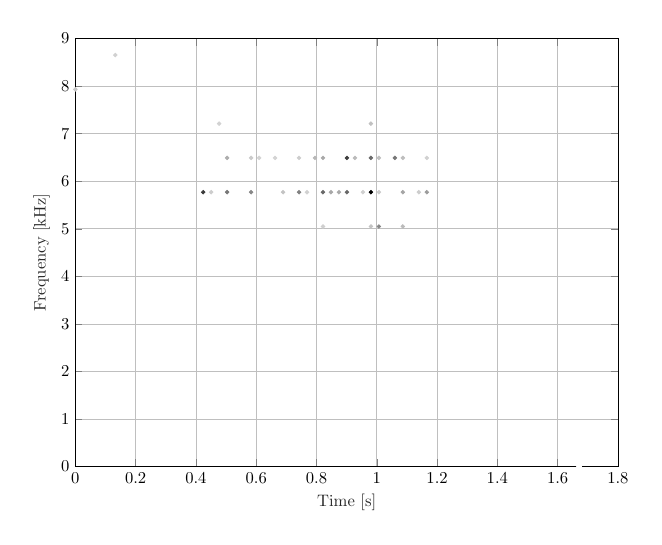
\begin{tikzpicture}[scale=0.6]

\begin{axis}[%
width=4.521in,
height=3.566in,
at={(0.758in,0.481in)},
scale only axis,
colormap={mymap}{[1pt] rgb(0pt)=(1,1,1); rgb(63pt)=(0,0,0)},
xmin=0,
xmax=1.8,
xlabel style={font=\color{white!15!black}},
xlabel={Time [s]},
ymin=0,
ymax=9,
ylabel style={font=\color{white!15!black}},
ylabel={Frequency [kHz]},
axis background/.style={fill=white},
%axis x line*=bottom,
%axis y line*=left,
xmajorgrids,
ymajorgrids
]
\addplot[scatter, only marks, mark=*, mark size=1.1180pt, scatter src=explicit, scatter/use mapped color={mark options={}, draw=mapped color, fill=mapped color}] table[row sep=crcr, meta=color]{%
x	y	color\\
0	7.93239436619718	27090\\
0.1325	8.65352112676056	22120\\
0.424	5.76901408450704	93563\\
0.4505	5.76901408450704	23816\\
0.477	7.2112676056338	21491\\
0.5035	5.76901408450704	64183\\
0.5035	6.49014084507042	38560\\
0.583	5.76901408450704	56633\\
0.583	6.49014084507042	24974\\
0.6095	6.49014084507042	20956\\
0.6625	6.49014084507042	20504\\
0.689	5.76901408450704	28617\\
0.742	5.76901408450704	60332\\
0.742	6.49014084507042	23912\\
0.7685	5.76901408450704	21957\\
0.795	6.49014084507042	34049\\
0.8215	5.04788732394366	23102\\
0.8215	5.76901408450704	71753\\
0.8215	6.49014084507042	41109\\
0.848	5.76901408450704	41597\\
0.8745	5.76901408450704	40719\\
0.901	5.76901408450704	72028\\
0.901	6.49014084507042	91240\\
0.9275	6.49014084507042	32283\\
0.954	5.76901408450704	22412\\
0.9805	5.04788732394366	28866\\
0.9805	5.76901408450704	121662\\
0.9805	6.49014084507042	70415\\
0.9805	7.2112676056338	29626\\
0.9805	18.0281690140845	29206\\
1.007	5.04788732394366	57621\\
1.007	5.76901408450704	24125\\
1.007	6.49014084507042	29975\\
1.06	6.49014084507042	64440\\
1.0865	5.04788732394366	32598\\
1.0865	5.76901408450704	43150\\
1.0865	6.49014084507042	31142\\
1.1395	5.76901408450704	23718\\
1.166	5.76901408450704	47450\\
1.166	6.49014084507042	22177\\
1.6715	0	0\\
1.6715	0	0\\
1.6715	0	0\\
1.6715	0	0\\
1.6715	0	0\\
1.6715	0	0\\
1.6715	0	0\\
1.6715	0	0\\
1.6715	0	0\\
1.6715	0	0\\
1.6715	0	0\\
1.6715	0	0\\
1.6715	0	0\\
1.6715	0	0\\
1.6715	0	0\\
1.6715	0	0\\
1.6715	0	0\\
1.6715	0	0\\
1.6715	0	0\\
1.6715	0	0\\
1.6715	0	0\\
1.6715	0	0\\
1.6715	0	0\\
1.6715	0	0\\
1.6715	0	0\\
1.6715	0	0\\
1.6715	0	0\\
1.6715	0	0\\
1.6715	0	0\\
1.6715	0	0\\
1.6715	0	0\\
1.6715	0	0\\
1.6715	0	0\\
1.6715	0	0\\
1.6715	0	0\\
1.6715	0	0\\
1.6715	0	0\\
1.6715	0	0\\
1.6715	0	0\\
1.6715	0	0\\
1.6715	0	0\\
1.6715	0	0\\
1.6715	0	0\\
1.6715	0	0\\
1.6715	0	0\\
1.6715	0	0\\
1.6715	0	0\\
1.6715	0	0\\
1.6715	0	0\\
1.6715	0	0\\
1.6715	0	0\\
1.6715	0	0\\
1.6715	0	0\\
1.6715	0	0\\
1.6715	0	0\\
1.6715	0	0\\
1.6715	0	0\\
1.6715	0	0\\
1.6715	0	0\\
1.6715	0	0\\
1.6715	0	0\\
1.6715	0	0\\
1.6715	0	0\\
1.6715	0	0\\
1.6715	0	0\\
1.6715	0	0\\
1.6715	0	0\\
1.6715	0	0\\
1.6715	0	0\\
1.6715	0	0\\
1.6715	0	0\\
1.6715	0	0\\
1.6715	0	0\\
1.6715	0	0\\
1.6715	0	0\\
1.6715	0	0\\
1.6715	0	0\\
1.6715	0	0\\
1.6715	0	0\\
1.6715	0	0\\
1.6715	0	0\\
1.6715	0	0\\
1.6715	0	0\\
1.6715	0	0\\
1.6715	0	0\\
1.6715	0	0\\
1.6715	0	0\\
1.6715	0	0\\
1.6715	0	0\\
1.6715	0	0\\
1.6715	0	0\\
1.6715	0	0\\
1.6715	0	0\\
1.6715	0	0\\
1.6715	0	0\\
1.6715	0	0\\
1.6715	0	0\\
1.6715	0	0\\
1.6715	0	0\\
1.6715	0	0\\
1.6715	0	0\\
1.6715	0	0\\
1.6715	0	0\\
1.6715	0	0\\
1.6715	0	0\\
1.6715	0	0\\
1.6715	0	0\\
1.6715	0	0\\
1.6715	0	0\\
1.6715	0	0\\
1.6715	0	0\\
1.6715	0	0\\
1.6715	0	0\\
1.6715	0	0\\
1.6715	0	0\\
1.6715	0	0\\
1.6715	0	0\\
1.6715	0	0\\
1.6715	0	0\\
1.6715	0	0\\
1.6715	0	0\\
1.6715	0	0\\
1.6715	0	0\\
1.6715	0	0\\
1.6715	0	0\\
1.6715	0	0\\
1.6715	0	0\\
1.6715	0	0\\
1.6715	0	0\\
1.6715	0	0\\
1.6715	0	0\\
1.6715	0	0\\
1.6715	0	0\\
1.6715	0	0\\
1.6715	0	0\\
1.6715	0	0\\
1.6715	0	0\\
1.6715	0	0\\
1.6715	0	0\\
1.6715	0	0\\
1.6715	0	0\\
1.6715	0	0\\
1.6715	0	0\\
1.6715	0	0\\
1.6715	0	0\\
1.6715	0	0\\
1.6715	0	0\\
1.6715	0	0\\
1.6715	0	0\\
1.6715	0	0\\
1.6715	0	0\\
1.6715	0	0\\
1.6715	0	0\\
1.6715	0	0\\
1.6715	0	0\\
1.6715	0	0\\
1.6715	0	0\\
1.6715	0	0\\
1.6715	0	0\\
1.6715	0	0\\
};
\end{axis}
\end{tikzpicture}%

  \caption{Bird song}
\end{subfigure}
\caption{Spectrograms of two sounds from the blue tit computed with this sensor node}
\label{fig:blue_tit}
\end{figure}

Due to the limited memory, the signal has to be processed at each time window. This considerably increases the delay between adjacent time windows, given by \SI{26.5}{ms} for an FFT size of $N = 128$ (see Table~\ref{tab:spec_data_proc}).

\begin{table}[H]
\centering
\begin{tabular}{lc}
\toprule
                     & Time [\si{ms}] \\ \midrule
 Data sampling       & 1.28           \\
 FFT                 & 25             \\
 Data storage        & 0.2            \\ \midrule
 Total               & 26.5           \\ \bottomrule
\end{tabular}
\caption{Processing time for one spectrogram data chunk with 128 samples}
\label{tab:spec_data_proc}
\end{table}

In this case, the sampling period is set to \SI{10}{\micro s}, corresponding to a sampling frequency $f_\te{s} = \SI{100}{kHz}$. Hence, the frequency resolution in the spectrogram is given by
\[
 \Delta f = \frac{f_\te{s}}{N} = \SI{781}{Hz}
\]
with a maximum analyzed frequency of $f_\te{s}/2 = \SI{50}{kHz}$. One can finally see the trade-off appearing on the frequency resolution, which cannot be improved (that is, decreased) without 
\begin{itemize}
 \item increasing $N$, which would require more memory storage and processing time (the FFT time evolving according to $\mathcal{O}(N^2)$, or $\mathcal{O}(N \log N)$ with optimized algorithms~\cite{QIU1999159}),
 \item or decreasing $f_\te{s}$, which would increase the sampling time (impinging on the time window length).
\end{itemize}

Figure~\ref{fig:4birds} provides the time--frequency comparison of four different bird songs. As discussed, the frequency resolution is also \SI{781}{Hz}. This makes discrimination among the birds very difficult since some peak frequencies are identical for several birds.

\begin{figure}[H]
\begin{subfigure}{.49\textwidth}
  \centering
  % This file was created by matlab2tikz.
%
%The latest updates can be retrieved from
%  http://www.mathworks.com/matlabcentral/fileexchange/22022-matlab2tikz-matlab2tikz
%where you can also make suggestions and rate matlab2tikz.
%
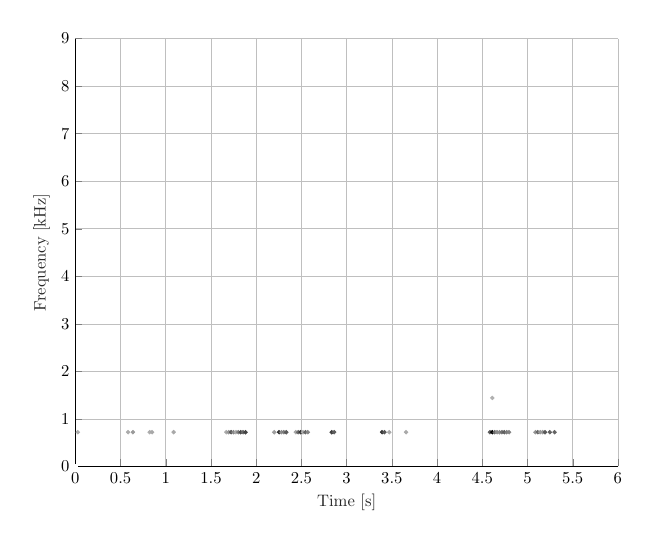
\begin{tikzpicture}[scale=0.6]

\begin{axis}[%
width=4.521in,
height=3.566in,
at={(0.758in,0.481in)},
scale only axis,
colormap={mymap}{[1pt] rgb(0pt)=(1,1,1); rgb(63pt)=(0,0,0)},
xmin=0,
xmax=6,
xlabel style={font=\color{white!15!black}},
xlabel={Time [s]},
ymin=0,
ymax=9,
ylabel style={font=\color{white!15!black}},
ylabel={Frequency [kHz]},
axis background/.style={fill=white},
axis x line*=bottom,
axis y line*=left,
xmajorgrids,
ymajorgrids
]
\addplot[scatter, only marks, mark=*, mark size=1.1180pt, scatter src=explicit, scatter/use mapped color={mark options={}, draw=mapped color, fill=mapped color}] table[row sep=crcr, meta=color]{%
x	y	color\\
0.0265	0.72112676056338	21138\\
0.583	0.72112676056338	21261\\
0.636	0.72112676056338	25889\\
0.8215	0.72112676056338	20975\\
0.848	0.72112676056338	22213\\
1.0865	0.72112676056338	22249\\
1.6695	0.72112676056338	21634\\
1.696	0.72112676056338	26913\\
1.7225	0.72112676056338	42656\\
1.749	0.72112676056338	30722\\
1.7755	0.72112676056338	21636\\
1.802	0.72112676056338	33312\\
1.8285	0.72112676056338	46743\\
1.855	0.72112676056338	39194\\
1.8815	0.72112676056338	48087\\
2.1995	0.72112676056338	24839\\
2.2525	0.72112676056338	52750\\
2.279	0.72112676056338	29295\\
2.3055	0.72112676056338	33029\\
2.332	0.72112676056338	42123\\
2.438	0.72112676056338	22693\\
2.4645	0.72112676056338	38214\\
2.491	0.72112676056338	52032\\
2.5175	0.72112676056338	21975\\
2.544	0.72112676056338	39835\\
2.5705	0.72112676056338	31398\\
2.8355	0.72112676056338	48815\\
2.862	0.72112676056338	41474\\
3.392	0.72112676056338	51363\\
3.4185	0.72112676056338	42949\\
3.4715	0.72112676056338	21607\\
3.657	0.72112676056338	21741\\
4.5845	0.72112676056338	41183\\
4.611	0.72112676056338	65299\\
4.611	1.44225352112676	20318\\
4.6375	0.72112676056338	38279\\
4.664	0.72112676056338	29414\\
4.6905	0.72112676056338	29178\\
4.717	0.72112676056338	36067\\
4.7435	0.72112676056338	41519\\
4.77	0.72112676056338	33884\\
4.7965	0.72112676056338	31981\\
5.088	0.72112676056338	27174\\
5.1145	0.72112676056338	38879\\
5.141	0.72112676056338	26662\\
5.1675	0.72112676056338	25562\\
5.194	0.72112676056338	42210\\
5.247	0.72112676056338	40518\\
5.3	0.72112676056338	39807\\
0	0	0\\
0	0	0\\
0	0	0\\
0	0	0\\
0	0	0\\
0	0	0\\
0	0	0\\
0	0	0\\
0	0	0\\
0	0	0\\
0	0	0\\
0	0	0\\
0	0	0\\
0	0	0\\
0	0	0\\
0	0	0\\
0	0	0\\
0	0	0\\
0	0	0\\
0	0	0\\
0	0	0\\
0	0	0\\
0	0	0\\
0	0	0\\
0	0	0\\
0	0	0\\
0	0	0\\
0	0	0\\
0	0	0\\
0	0	0\\
0	0	0\\
0	0	0\\
0	0	0\\
0	0	0\\
0	0	0\\
0	0	0\\
0	0	0\\
0	0	0\\
0	0	0\\
0	0	0\\
0	0	0\\
0	0	0\\
0	0	0\\
0	0	0\\
0	0	0\\
0	0	0\\
0	0	0\\
0	0	0\\
0	0	0\\
0	0	0\\
0	0	0\\
0	0	0\\
0	0	0\\
0	0	0\\
0	0	0\\
0	0	0\\
0	0	0\\
0	0	0\\
0	0	0\\
0	0	0\\
0	0	0\\
0	0	0\\
0	0	0\\
0	0	0\\
0	0	0\\
0	0	0\\
0	0	0\\
0	0	0\\
0	0	0\\
0	0	0\\
0	0	0\\
0	0	0\\
0	0	0\\
0	0	0\\
0	0	0\\
0	0	0\\
0	0	0\\
0	0	0\\
0	0	0\\
0	0	0\\
0	0	0\\
0	0	0\\
0	0	0\\
0	0	0\\
0	0	0\\
0	0	0\\
0	0	0\\
0	0	0\\
0	0	0\\
0	0	0\\
0	0	0\\
0	0	0\\
0	0	0\\
0	0	0\\
0	0	0\\
0	0	0\\
0	0	0\\
0	0	0\\
0	0	0\\
0	0	0\\
0	0	0\\
0	0	0\\
0	0	0\\
0	0	0\\
0	0	0\\
0	0	0\\
0	0	0\\
0	0	0\\
0	0	0\\
0	0	0\\
0	0	0\\
0	0	0\\
0	0	0\\
0	0	0\\
0	0	0\\
0	0	0\\
0	0	0\\
0	0	0\\
0	0	0\\
0	0	0\\
0	0	0\\
0	0	0\\
0	0	0\\
0	0	0\\
0	0	0\\
0	0	0\\
0	0	0\\
0	0	0\\
0	0	0\\
0	0	0\\
0	0	0\\
0	0	0\\
0	0	0\\
0	0	0\\
0	0	0\\
0	0	0\\
0	0	0\\
0	0	0\\
0	0	0\\
0	0	0\\
0	0	0\\
0	0	0\\
0	0	0\\
0	0	0\\
0	0	0\\
0	0	0\\
0	0	0\\
0	0	0\\
0	0	0\\
0	0	0\\
0	0	0\\
};
\end{axis}
\end{tikzpicture}%

  \caption{Pigeon}
\end{subfigure}
\begin{subfigure}{.49\textwidth}
  \centering
  % This file was created by matlab2tikz.
%
%The latest updates can be retrieved from
%  http://www.mathworks.com/matlabcentral/fileexchange/22022-matlab2tikz-matlab2tikz
%where you can also make suggestions and rate matlab2tikz.
%
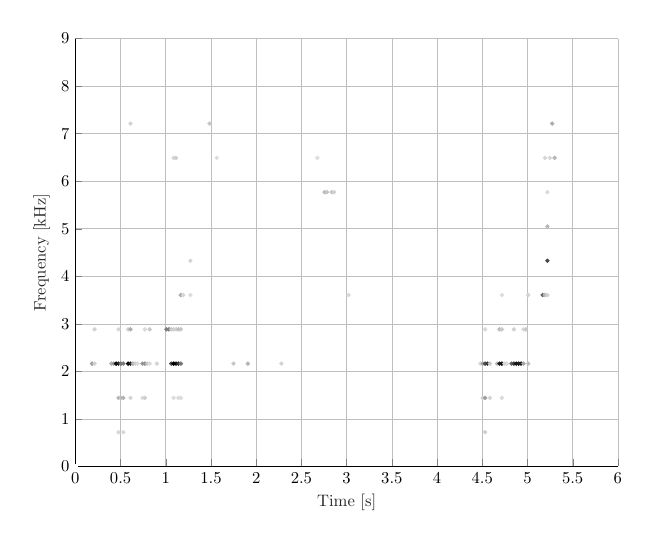
\begin{tikzpicture}[scale=0.6]

\begin{axis}[%
width=4.521in,
height=3.566in,
at={(0.758in,0.481in)},
scale only axis,
colormap={mymap}{[1pt] rgb(0pt)=(1,1,1); rgb(63pt)=(0,0,0)},
xmin=0,
xmax=6,
xlabel style={font=\color{white!15!black}},
xlabel={Time [s]},
ymin=0,
ymax=9,
ylabel style={font=\color{white!15!black}},
ylabel={Frequency [kHz]},
axis background/.style={fill=white},
axis x line*=bottom,
axis y line*=left,
xmajorgrids,
ymajorgrids
]
\addplot[scatter, only marks, mark=*, mark size=1.1180pt, scatter src=explicit, scatter/use mapped color={mark options={}, draw=mapped color, fill=mapped color}] table[row sep=crcr, meta=color]{%
x	y	color\\
0.1855	2.16338028169014	58966\\
0.212	2.16338028169014	27500\\
0.212	2.88450704225352	27649\\
0.3975	2.16338028169014	45945\\
0.424	2.16338028169014	59554\\
0.4505	2.16338028169014	145040\\
0.477	0.72112676056338	22792\\
0.477	1.44225352112676	44677\\
0.477	2.16338028169014	132405\\
0.477	2.88450704225352	24698\\
0.5035	1.44225352112676	37410\\
0.5035	2.16338028169014	81456\\
0.53	0.72112676056338	22943\\
0.53	1.44225352112676	46290\\
0.53	2.16338028169014	76792\\
0.583	2.16338028169014	143057\\
0.583	2.88450704225352	26180\\
0.6095	1.44225352112676	26230\\
0.6095	2.16338028169014	135568\\
0.6095	2.88450704225352	47292\\
0.6095	7.2112676056338	25844\\
0.636	2.16338028169014	46659\\
0.6625	2.16338028169014	28604\\
0.689	2.16338028169014	21078\\
0.742	1.44225352112676	20582\\
0.742	2.16338028169014	60726\\
0.7685	1.44225352112676	28343\\
0.7685	2.16338028169014	64834\\
0.7685	2.88450704225352	22092\\
0.795	2.16338028169014	34214\\
0.8215	2.16338028169014	21941\\
0.8215	2.88450704225352	32151\\
0.901	2.16338028169014	24576\\
1.007	2.88450704225352	74942\\
1.0335	2.88450704225352	76339\\
1.06	2.16338028169014	109826\\
1.06	2.88450704225352	33101\\
1.0865	1.44225352112676	20436\\
1.0865	2.16338028169014	149433\\
1.0865	2.88450704225352	27847\\
1.0865	6.49014084507042	23949\\
1.113	2.16338028169014	149021\\
1.113	2.88450704225352	27364\\
1.113	6.49014084507042	29176\\
1.1395	1.44225352112676	21798\\
1.1395	2.16338028169014	120972\\
1.1395	2.88450704225352	37533\\
1.166	1.44225352112676	20500\\
1.166	2.16338028169014	80271\\
1.166	2.88450704225352	34797\\
1.166	3.6056338028169	50589\\
1.1925	3.6056338028169	23959\\
1.272	3.6056338028169	20644\\
1.272	4.32676056338028	25195\\
1.484	7.2112676056338	32758\\
1.5635	6.49014084507042	20270\\
1.749	2.16338028169014	33325\\
1.908	2.16338028169014	43189\\
2.279	2.16338028169014	25159\\
2.6765	6.49014084507042	20137\\
2.756	5.76901408450704	40386\\
2.7825	5.76901408450704	33874\\
2.8355	5.76901408450704	34062\\
2.862	5.76901408450704	27125\\
3.021	3.6056338028169	23527\\
4.4785	2.16338028169014	22614\\
4.505	1.44225352112676	28957\\
4.505	2.16338028169014	55718\\
4.5315	0.72112676056338	27969\\
4.5315	1.44225352112676	55723\\
4.5315	2.16338028169014	105508\\
4.5315	2.88450704225352	22625\\
4.558	2.16338028169014	120198\\
4.5845	1.44225352112676	24451\\
4.5845	2.16338028169014	32815\\
4.664	2.16338028169014	41476\\
4.6905	2.16338028169014	132156\\
4.6905	2.88450704225352	39642\\
4.717	1.44225352112676	20932\\
4.717	2.16338028169014	141254\\
4.717	2.88450704225352	31043\\
4.717	3.6056338028169	20132\\
4.7435	2.16338028169014	26088\\
4.77	2.16338028169014	22715\\
4.823	2.16338028169014	89253\\
4.8495	2.16338028169014	113300\\
4.8495	2.88450704225352	27386\\
4.876	2.16338028169014	140729\\
4.9025	2.16338028169014	131259\\
4.929	2.16338028169014	133784\\
4.9555	2.16338028169014	52506\\
4.9555	2.88450704225352	21931\\
4.982	2.88450704225352	32053\\
5.0085	2.16338028169014	40392\\
5.0085	3.6056338028169	24750\\
5.1675	3.6056338028169	91287\\
5.194	3.6056338028169	42020\\
5.194	6.49014084507042	24769\\
5.2205	3.6056338028169	27312\\
5.2205	4.32676056338028	108834\\
5.2205	5.04788732394366	41668\\
5.2205	5.76901408450704	21677\\
5.247	6.49014084507042	22621\\
5.2735	7.2112676056338	48387\\
5.3	6.49014084507042	43210\\
0	0	0\\
0	0	0\\
0	0	0\\
0	0	0\\
0	0	0\\
0	0	0\\
0	0	0\\
0	0	0\\
0	0	0\\
0	0	0\\
0	0	0\\
0	0	0\\
0	0	0\\
0	0	0\\
0	0	0\\
0	0	0\\
0	0	0\\
0	0	0\\
0	0	0\\
0	0	0\\
0	0	0\\
0	0	0\\
0	0	0\\
0	0	0\\
0	0	0\\
0	0	0\\
0	0	0\\
0	0	0\\
0	0	0\\
0	0	0\\
0	0	0\\
0	0	0\\
0	0	0\\
0	0	0\\
0	0	0\\
0	0	0\\
0	0	0\\
0	0	0\\
0	0	0\\
0	0	0\\
0	0	0\\
0	0	0\\
0	0	0\\
0	0	0\\
0	0	0\\
0	0	0\\
0	0	0\\
0	0	0\\
0	0	0\\
0	0	0\\
0	0	0\\
0	0	0\\
0	0	0\\
0	0	0\\
0	0	0\\
0	0	0\\
0	0	0\\
0	0	0\\
0	0	0\\
0	0	0\\
0	0	0\\
0	0	0\\
0	0	0\\
0	0	0\\
0	0	0\\
0	0	0\\
0	0	0\\
0	0	0\\
0	0	0\\
0	0	0\\
0	0	0\\
0	0	0\\
0	0	0\\
0	0	0\\
0	0	0\\
0	0	0\\
0	0	0\\
0	0	0\\
0	0	0\\
0	0	0\\
0	0	0\\
0	0	0\\
0	0	0\\
0	0	0\\
0	0	0\\
0	0	0\\
0	0	0\\
0	0	0\\
0	0	0\\
0	0	0\\
0	0	0\\
0	0	0\\
0	0	0\\
0	0	0\\
0	0	0\\
};
\end{axis}
\end{tikzpicture}%

  \caption{Blackbird}
\end{subfigure}
\newline
\begin{subfigure}{.49\textwidth}
  \centering
  % This file was created by matlab2tikz.
%
%The latest updates can be retrieved from
%  http://www.mathworks.com/matlabcentral/fileexchange/22022-matlab2tikz-matlab2tikz
%where you can also make suggestions and rate matlab2tikz.
%
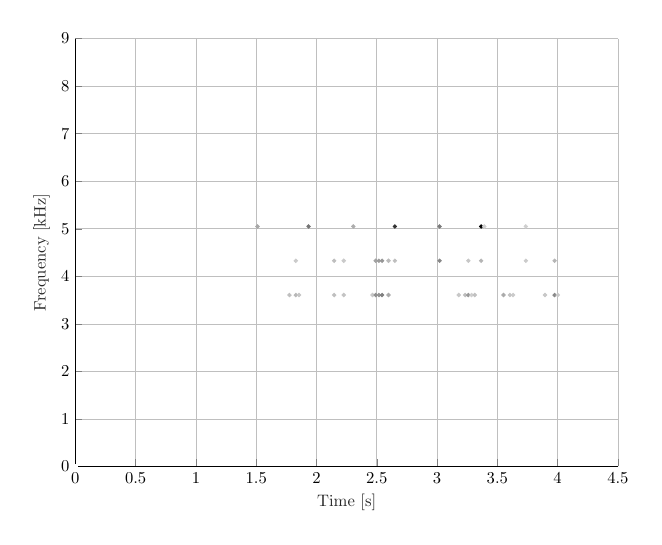
\begin{tikzpicture}[scale=0.6]

\begin{axis}[%
width=4.521in,
height=3.566in,
at={(0.758in,0.481in)},
scale only axis,
colormap={mymap}{[1pt] rgb(0pt)=(1,1,1); rgb(63pt)=(0,0,0)},
xmin=0,
xmax=4.5,
xlabel style={font=\color{white!15!black}},
xlabel={Time [s]},
ymin=0,
ymax=9,
ylabel style={font=\color{white!15!black}},
ylabel={Frequency [kHz]},
axis background/.style={fill=white},
axis x line*=bottom,
axis y line*=left,
xmajorgrids,
ymajorgrids
]
\addplot[scatter, only marks, mark=*, mark size=1.1180pt, scatter src=explicit, scatter/use mapped color={mark options={}, draw=mapped color, fill=mapped color}] table[row sep=crcr, meta=color]{%
x	y	color\\
1.5105	5.04788732394366	37306\\
1.7755	3.6056338028169	27352\\
1.8285	3.6056338028169	30612\\
1.8285	4.32676056338028	22268\\
1.855	3.6056338028169	23863\\
1.9345	5.04788732394366	59246\\
2.1465	3.6056338028169	27606\\
2.1465	4.32676056338028	27882\\
2.226	3.6056338028169	25177\\
2.226	4.32676056338028	22946\\
2.3055	5.04788732394366	35298\\
2.4645	3.6056338028169	24203\\
2.491	3.6056338028169	47774\\
2.491	4.32676056338028	39423\\
2.5175	3.6056338028169	45709\\
2.5175	4.32676056338028	42397\\
2.544	3.6056338028169	54545\\
2.544	4.32676056338028	44784\\
2.597	3.6056338028169	37115\\
2.597	4.32676056338028	29121\\
2.65	4.32676056338028	28091\\
2.65	5.04788732394366	88128\\
3.021	4.32676056338028	50985\\
3.021	5.04788732394366	56884\\
3.18	3.6056338028169	23785\\
3.233	3.6056338028169	28288\\
3.2595	3.6056338028169	44413\\
3.2595	4.32676056338028	24254\\
3.286	3.6056338028169	20647\\
3.3125	3.6056338028169	26675\\
3.3655	4.32676056338028	32076\\
3.3655	5.04788732394366	109589\\
3.392	5.04788732394366	20206\\
3.551	3.6056338028169	36560\\
3.604	3.6056338028169	25435\\
3.6305	3.6056338028169	22539\\
3.7365	4.32676056338028	22141\\
3.7365	5.04788732394366	20487\\
3.8955	3.6056338028169	23480\\
3.975	3.6056338028169	50776\\
3.975	4.32676056338028	31713\\
4.0015	3.6056338028169	23158\\
0	0	0\\
0	0	0\\
0	0	0\\
0	0	0\\
0	0	0\\
0	0	0\\
0	0	0\\
0	0	0\\
0	0	0\\
0	0	0\\
0	0	0\\
0	0	0\\
0	0	0\\
0	0	0\\
0	0	0\\
0	0	0\\
0	0	0\\
0	0	0\\
0	0	0\\
0	0	0\\
0	0	0\\
0	0	0\\
0	0	0\\
0	0	0\\
0	0	0\\
0	0	0\\
0	0	0\\
0	0	0\\
0	0	0\\
0	0	0\\
0	0	0\\
0	0	0\\
0	0	0\\
0	0	0\\
0	0	0\\
0	0	0\\
0	0	0\\
0	0	0\\
0	0	0\\
0	0	0\\
0	0	0\\
0	0	0\\
0	0	0\\
0	0	0\\
0	0	0\\
0	0	0\\
0	0	0\\
0	0	0\\
0	0	0\\
0	0	0\\
0	0	0\\
0	0	0\\
0	0	0\\
0	0	0\\
0	0	0\\
0	0	0\\
0	0	0\\
0	0	0\\
0	0	0\\
0	0	0\\
0	0	0\\
0	0	0\\
0	0	0\\
0	0	0\\
0	0	0\\
0	0	0\\
0	0	0\\
0	0	0\\
0	0	0\\
0	0	0\\
0	0	0\\
0	0	0\\
0	0	0\\
0	0	0\\
0	0	0\\
0	0	0\\
0	0	0\\
0	0	0\\
0	0	0\\
0	0	0\\
0	0	0\\
0	0	0\\
0	0	0\\
0	0	0\\
0	0	0\\
0	0	0\\
0	0	0\\
0	0	0\\
0	0	0\\
0	0	0\\
0	0	0\\
0	0	0\\
0	0	0\\
0	0	0\\
0	0	0\\
0	0	0\\
0	0	0\\
0	0	0\\
0	0	0\\
0	0	0\\
0	0	0\\
0	0	0\\
0	0	0\\
0	0	0\\
0	0	0\\
0	0	0\\
0	0	0\\
0	0	0\\
0	0	0\\
0	0	0\\
0	0	0\\
0	0	0\\
0	0	0\\
0	0	0\\
0	0	0\\
0	0	0\\
0	0	0\\
0	0	0\\
0	0	0\\
0	0	0\\
0	0	0\\
0	0	0\\
0	0	0\\
0	0	0\\
0	0	0\\
0	0	0\\
0	0	0\\
0	0	0\\
0	0	0\\
0	0	0\\
0	0	0\\
0	0	0\\
0	0	0\\
0	0	0\\
0	0	0\\
0	0	0\\
0	0	0\\
0	0	0\\
0	0	0\\
0	0	0\\
0	0	0\\
0	0	0\\
0	0	0\\
0	0	0\\
0	0	0\\
0	0	0\\
0	0	0\\
0	0	0\\
0	0	0\\
0	0	0\\
0	0	0\\
0	0	0\\
0	0	0\\
0	0	0\\
0	0	0\\
0	0	0\\
0	0	0\\
0	0	0\\
};
\end{axis}
\end{tikzpicture}%

  \caption{Great tit}
  \label{fig:great_tit}
\end{subfigure}
\begin{subfigure}{.49\textwidth}
  \centering
  % This file was created by matlab2tikz.
%
%The latest updates can be retrieved from
%  http://www.mathworks.com/matlabcentral/fileexchange/22022-matlab2tikz-matlab2tikz
%where you can also make suggestions and rate matlab2tikz.
%
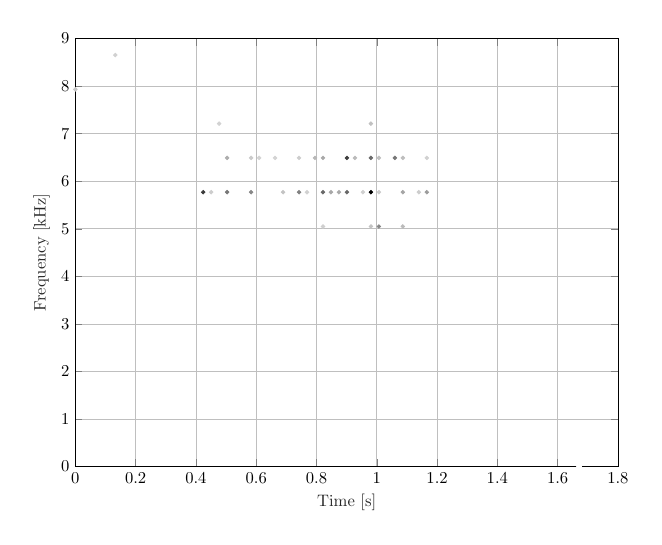
\begin{tikzpicture}[scale=0.6]

\begin{axis}[%
width=4.521in,
height=3.566in,
at={(0.758in,0.481in)},
scale only axis,
colormap={mymap}{[1pt] rgb(0pt)=(1,1,1); rgb(63pt)=(0,0,0)},
xmin=0,
xmax=1.8,
xlabel style={font=\color{white!15!black}},
xlabel={Time [s]},
ymin=0,
ymax=9,
ylabel style={font=\color{white!15!black}},
ylabel={Frequency [kHz]},
axis background/.style={fill=white},
%axis x line*=bottom,
%axis y line*=left,
xmajorgrids,
ymajorgrids
]
\addplot[scatter, only marks, mark=*, mark size=1.1180pt, scatter src=explicit, scatter/use mapped color={mark options={}, draw=mapped color, fill=mapped color}] table[row sep=crcr, meta=color]{%
x	y	color\\
0	7.93239436619718	27090\\
0.1325	8.65352112676056	22120\\
0.424	5.76901408450704	93563\\
0.4505	5.76901408450704	23816\\
0.477	7.2112676056338	21491\\
0.5035	5.76901408450704	64183\\
0.5035	6.49014084507042	38560\\
0.583	5.76901408450704	56633\\
0.583	6.49014084507042	24974\\
0.6095	6.49014084507042	20956\\
0.6625	6.49014084507042	20504\\
0.689	5.76901408450704	28617\\
0.742	5.76901408450704	60332\\
0.742	6.49014084507042	23912\\
0.7685	5.76901408450704	21957\\
0.795	6.49014084507042	34049\\
0.8215	5.04788732394366	23102\\
0.8215	5.76901408450704	71753\\
0.8215	6.49014084507042	41109\\
0.848	5.76901408450704	41597\\
0.8745	5.76901408450704	40719\\
0.901	5.76901408450704	72028\\
0.901	6.49014084507042	91240\\
0.9275	6.49014084507042	32283\\
0.954	5.76901408450704	22412\\
0.9805	5.04788732394366	28866\\
0.9805	5.76901408450704	121662\\
0.9805	6.49014084507042	70415\\
0.9805	7.2112676056338	29626\\
0.9805	18.0281690140845	29206\\
1.007	5.04788732394366	57621\\
1.007	5.76901408450704	24125\\
1.007	6.49014084507042	29975\\
1.06	6.49014084507042	64440\\
1.0865	5.04788732394366	32598\\
1.0865	5.76901408450704	43150\\
1.0865	6.49014084507042	31142\\
1.1395	5.76901408450704	23718\\
1.166	5.76901408450704	47450\\
1.166	6.49014084507042	22177\\
1.6715	0	0\\
1.6715	0	0\\
1.6715	0	0\\
1.6715	0	0\\
1.6715	0	0\\
1.6715	0	0\\
1.6715	0	0\\
1.6715	0	0\\
1.6715	0	0\\
1.6715	0	0\\
1.6715	0	0\\
1.6715	0	0\\
1.6715	0	0\\
1.6715	0	0\\
1.6715	0	0\\
1.6715	0	0\\
1.6715	0	0\\
1.6715	0	0\\
1.6715	0	0\\
1.6715	0	0\\
1.6715	0	0\\
1.6715	0	0\\
1.6715	0	0\\
1.6715	0	0\\
1.6715	0	0\\
1.6715	0	0\\
1.6715	0	0\\
1.6715	0	0\\
1.6715	0	0\\
1.6715	0	0\\
1.6715	0	0\\
1.6715	0	0\\
1.6715	0	0\\
1.6715	0	0\\
1.6715	0	0\\
1.6715	0	0\\
1.6715	0	0\\
1.6715	0	0\\
1.6715	0	0\\
1.6715	0	0\\
1.6715	0	0\\
1.6715	0	0\\
1.6715	0	0\\
1.6715	0	0\\
1.6715	0	0\\
1.6715	0	0\\
1.6715	0	0\\
1.6715	0	0\\
1.6715	0	0\\
1.6715	0	0\\
1.6715	0	0\\
1.6715	0	0\\
1.6715	0	0\\
1.6715	0	0\\
1.6715	0	0\\
1.6715	0	0\\
1.6715	0	0\\
1.6715	0	0\\
1.6715	0	0\\
1.6715	0	0\\
1.6715	0	0\\
1.6715	0	0\\
1.6715	0	0\\
1.6715	0	0\\
1.6715	0	0\\
1.6715	0	0\\
1.6715	0	0\\
1.6715	0	0\\
1.6715	0	0\\
1.6715	0	0\\
1.6715	0	0\\
1.6715	0	0\\
1.6715	0	0\\
1.6715	0	0\\
1.6715	0	0\\
1.6715	0	0\\
1.6715	0	0\\
1.6715	0	0\\
1.6715	0	0\\
1.6715	0	0\\
1.6715	0	0\\
1.6715	0	0\\
1.6715	0	0\\
1.6715	0	0\\
1.6715	0	0\\
1.6715	0	0\\
1.6715	0	0\\
1.6715	0	0\\
1.6715	0	0\\
1.6715	0	0\\
1.6715	0	0\\
1.6715	0	0\\
1.6715	0	0\\
1.6715	0	0\\
1.6715	0	0\\
1.6715	0	0\\
1.6715	0	0\\
1.6715	0	0\\
1.6715	0	0\\
1.6715	0	0\\
1.6715	0	0\\
1.6715	0	0\\
1.6715	0	0\\
1.6715	0	0\\
1.6715	0	0\\
1.6715	0	0\\
1.6715	0	0\\
1.6715	0	0\\
1.6715	0	0\\
1.6715	0	0\\
1.6715	0	0\\
1.6715	0	0\\
1.6715	0	0\\
1.6715	0	0\\
1.6715	0	0\\
1.6715	0	0\\
1.6715	0	0\\
1.6715	0	0\\
1.6715	0	0\\
1.6715	0	0\\
1.6715	0	0\\
1.6715	0	0\\
1.6715	0	0\\
1.6715	0	0\\
1.6715	0	0\\
1.6715	0	0\\
1.6715	0	0\\
1.6715	0	0\\
1.6715	0	0\\
1.6715	0	0\\
1.6715	0	0\\
1.6715	0	0\\
1.6715	0	0\\
1.6715	0	0\\
1.6715	0	0\\
1.6715	0	0\\
1.6715	0	0\\
1.6715	0	0\\
1.6715	0	0\\
1.6715	0	0\\
1.6715	0	0\\
1.6715	0	0\\
1.6715	0	0\\
1.6715	0	0\\
1.6715	0	0\\
1.6715	0	0\\
1.6715	0	0\\
1.6715	0	0\\
1.6715	0	0\\
1.6715	0	0\\
1.6715	0	0\\
1.6715	0	0\\
1.6715	0	0\\
1.6715	0	0\\
1.6715	0	0\\
1.6715	0	0\\
1.6715	0	0\\
1.6715	0	0\\
1.6715	0	0\\
1.6715	0	0\\
};
\end{axis}
\end{tikzpicture}%

  \caption{Blue tit}
\end{subfigure}
\caption{Spectrograms of four different bird songs computed with this sensor node}
\label{fig:4birds}
\end{figure}

To illustrate the difference, Figure~\ref{fig:greattit_full} shows the spectrogram of the great tit when the signal does not significantly suffer from the time-frequency trade-off (that is, the graph has been computed in offline mode from an audio file at \SI{44.1}{kHz}). One can clearly see four songs oscillating between \SI{3}{kHz} and \SI{6}{kHz}, which is not detected by the embedded low-resource microcontroller (see Figure~\ref{fig:great_tit}). It will thus be needed to work on specific characteristics of the signal instead of the whole spectrogram pattern.

\begin{figure}[H]
    \centering
    % This file was created by matlab2tikz.
%
%The latest updates can be retrieved from
%  http://www.mathworks.com/matlabcentral/fileexchange/22022-matlab2tikz-matlab2tikz
%where you can also make suggestions and rate matlab2tikz.
%
\begin{tikzpicture}

\begin{axis}[%
width=3.983in,
height=3.566in,
at={(0.668in,0.481in)},
scale only axis,
point meta min=-156.535557740088,
point meta max=-36.7993181309735,
axis on top,
xmin=0.00707482993197279,
xmax=34.3925623582766,
xlabel style={font=\color{white!15!black}},
xlabel={Time [s]},
ymin=-0.021533203125,
ymax=22.071533203125,
ylabel style={font=\color{white!15!black}},
ylabel={Frequency [kHz]},
axis background/.style={fill=white},
colormap={mymap}{[1pt] rgb(0pt)=(1,1,1); rgb(1pt)=(0.994681,0.994681,0.994681); rgb(2pt)=(0.989304,0.989304,0.989304); rgb(3pt)=(0.983868,0.983868,0.983868); rgb(4pt)=(0.978372,0.978372,0.978372); rgb(5pt)=(0.972813,0.972813,0.972813); rgb(6pt)=(0.967189,0.967189,0.967189); rgb(7pt)=(0.9615,0.9615,0.9615); rgb(8pt)=(0.955742,0.955742,0.955742); rgb(9pt)=(0.949914,0.949914,0.949914); rgb(10pt)=(0.944014,0.944014,0.944014); rgb(11pt)=(0.938039,0.938039,0.938039); rgb(12pt)=(0.931987,0.931987,0.931987); rgb(13pt)=(0.925855,0.925855,0.925855); rgb(14pt)=(0.919641,0.919641,0.919641); rgb(15pt)=(0.913342,0.913342,0.913342); rgb(16pt)=(0.906955,0.906955,0.906955); rgb(17pt)=(0.900477,0.900477,0.900477); rgb(18pt)=(0.893904,0.893904,0.893904); rgb(19pt)=(0.887232,0.887232,0.887232); rgb(20pt)=(0.880459,0.880459,0.880459); rgb(21pt)=(0.87358,0.87358,0.87358); rgb(22pt)=(0.866592,0.866592,0.866592); rgb(23pt)=(0.859488,0.859488,0.859488); rgb(24pt)=(0.852265,0.852265,0.852265); rgb(25pt)=(0.844918,0.844918,0.844918); rgb(26pt)=(0.83744,0.83744,0.83744); rgb(27pt)=(0.829827,0.829827,0.829827); rgb(28pt)=(0.822071,0.822071,0.822071); rgb(29pt)=(0.814166,0.814166,0.814166); rgb(30pt)=(0.806104,0.806104,0.806104); rgb(31pt)=(0.797878,0.797878,0.797878); rgb(32pt)=(0.789479,0.789479,0.789479); rgb(33pt)=(0.780897,0.780897,0.780897); rgb(34pt)=(0.772122,0.772122,0.772122); rgb(35pt)=(0.763143,0.763143,0.763143); rgb(36pt)=(0.753947,0.753947,0.753947); rgb(37pt)=(0.744522,0.744522,0.744522); rgb(38pt)=(0.734852,0.734852,0.734852); rgb(39pt)=(0.72492,0.72492,0.72492); rgb(40pt)=(0.714709,0.714709,0.714709); rgb(41pt)=(0.704197,0.704197,0.704197); rgb(42pt)=(0.693361,0.693361,0.693361); rgb(43pt)=(0.682176,0.682176,0.682176); rgb(44pt)=(0.670612,0.670612,0.670612); rgb(45pt)=(0.658634,0.658634,0.658634); rgb(46pt)=(0.646204,0.646204,0.646204); rgb(47pt)=(0.633276,0.633276,0.633276); rgb(48pt)=(0.619798,0.619798,0.619798); rgb(49pt)=(0.605707,0.605707,0.605707); rgb(50pt)=(0.590928,0.590928,0.590928); rgb(51pt)=(0.57537,0.57537,0.57537); rgb(52pt)=(0.558921,0.558921,0.558921); rgb(53pt)=(0.541444,0.541444,0.541444); rgb(54pt)=(0.522758,0.522758,0.522758); rgb(55pt)=(0.502632,0.502632,0.502632); rgb(56pt)=(0.48075,0.48075,0.48075); rgb(57pt)=(0.456671,0.456671,0.456671); rgb(58pt)=(0.429744,0.429744,0.429744); rgb(59pt)=(0.398939,0.398939,0.398939); rgb(60pt)=(0.36246,0.36246,0.36246); rgb(61pt)=(0.316638,0.316638,0.316638); rgb(62pt)=(0.251316,0.251316,0.251316); rgb(63pt)=(0,0,0)},
colorbar,
colorbar style={ylabel style={font=\color{white!15!black}}, ylabel={Power/frequency (dB/Hz)}}
]
\addplot [forget plot] graphics [xmin=0.00707482993197279, xmax=34.3925623582766, ymin=-0.021533203125, ymax=22.071533203125] {greattit_full-1.png};
\end{axis}
\end{tikzpicture}%
    \caption{Precise spectrogram of the great tit song (from a bird song database)}
    \label{fig:greattit_full}
\end{figure}

\subsubsection*{Feature extraction}

Now that the signal has been converted into meaningful information via its spectrogram form, some features need to be extracted from it. Typical features for bird recognition are specific frequencies for each time window, the median as well as the 5 and 95 percentiles which are robust measures of minimum and maximum frequency~\cite{Stowell}. The bandwidth can also be extracted, defined as the difference between the 5 and 95 percentiles. 

For this work, the average frequency weighted by the intensity is analyzed because of its simplicity and robustness. In a spectrogram, let $f[i]$ be the vector of discrete frequencies ($y$-axis) with size $N/2$, $t[j]$ be the vector of discrete time samples ($x$-axis) with size $M$ (depending on the audio recording time and the window overlap) and $s[i,j]$ be the intensity of the $i$-th frequency component during the $j$-th time period, then the average intensity for the $i$-th frequency component throughout the time period is
\[
 s_\te{avg}[i] = \frac{1}{M} \sum_{j=1}^{M} s[i,j] \quad [\si{dB/Hz}]
\]
and the weighted average frequency is given by
\[
 f_\te{avg} = \frac{\sum_{j=1}^{L} s_\te{avg}[i] \, f[i]}{\sum_{j=1}^{L} s_\te{avg}[i]} \quad [\si{Hz}]
\]
where $L$ is the index corresponding to a frequency of \SI{10}{kHz} in order to remove high-frequency noise from the average. The spectrogram has frequencies above this range if $f_\te{max} > \SI{10}{kHz}$, that is $f_\te{s} > \SI{20}{kHz}$. The sampling frequency is thus fixed to $f_\te{s} = \SI{20}{kHz}$ in order to remove significant noise while keeping the useful bandwidth of bird song (below \SI{10}{kHz}).

During calibration, the mean background noise (expressed as power spectral density) is characterized for each frequency, resulting in a combination of $1/f$ and white noise. It is then removed from the intensity $s[i,j]$ when a real signal is analyzed. The algorithm is also tuned by an intensity threshold to output a bird species only when the signal sufficiently exceeds the background noise, meaning that a sound has been produced.

\subsubsection*{Feature selection}

Additionally, feature selection is used to evaluate the predictive power that a feature has with respect to some attribute.
In information gain feature selection, each feature is evaluated by measuring the information gain with respect to the species label, which is the amount by which the feature reduces the uncertainty in the label. To reduce the problem complexity, the weighted average frequency is kept in this work. The problem thus becomes a 1D classification.

\subsubsection*{Inference}

The final step consists to infer the species based on the selected feature. A simple machine-learning model for this purpose is the support vector machine (SVM), but it requires much offline preprocessing beforehand. Since only one feature is analyzed, a complex machine-learning algorithm has little interest. The classifier used for this work is based on a $k$-nearest neighbors algorithm (KNN) with $k=5$, meaning that the class (i.e. the species) associated with a new sample is classified by a plurality vote among the $k$ nearest data according to the feature (i.e. the weighted average frequency).

A learning phase now consists to analyze several songs from the six species previously mentioned, and extract the weighted average frequency for all these learning samples. Figure~\ref{fig:weighted_average_frequency} shows the repartition of the weighted average frequency among the species learning samples, based on the spectrogram of six different audio samples for each species\footnote{The audio files come from a collaborative and open-source database of bird songs (\textit{xeno-canto}~\cite{xeno}).}.

\begin{figure}[H]
    \centering
    % This file was created by matlab2tikz.
%
%The latest updates can be retrieved from
%  http://www.mathworks.com/matlabcentral/fileexchange/22022-matlab2tikz-matlab2tikz
%where you can also make suggestions and rate matlab2tikz.
%
\definecolor{mycolor1}{rgb}{0.00000,0.44700,0.74100}%
\definecolor{mycolor2}{rgb}{0.85000,0.32500,0.09800}%
\definecolor{mycolor3}{rgb}{0.92900,0.69400,0.12500}%
\definecolor{mycolor4}{rgb}{0.49400,0.18400,0.55600}%
%
\begin{tikzpicture}

\begin{axis}[%
width=4.521in,
height=1.2in,
at={(0.758in,0.481in)},
scale only axis,
xmin=0,
xmax=7,
xlabel style={font=\color{white!15!black}},
xlabel={Weighted average frequency [kHz]},
ymin=0,
ymax=2.22044604925031e-16,
axis background/.style={fill=white},
axis x line*=bottom,
axis y line=none,
legend style={legend cell align=left, align=left, draw=none}
]
\addplot [color=mycolor1, draw=none, mark size=2.5pt, mark=*, mark options={solid, mycolor1}]
  table[row sep=crcr]{%
0.901579628386122	0\\
0.598078203756716	0\\
0.875811228066835	0\\
1.25038473443573	0\\
0.98976212228955	0\\
0.603235617097455	0\\
};
\addlegendentry{Pigeon}

\addplot [color=mycolor4, draw=none, mark size=2.5pt, mark=*, mark options={solid, mycolor4}]
  table[row sep=crcr]{%
2.78870571216995	0\\
2.9363029875264	0\\
2.60567527145653	0\\
2.01841901994883	0\\
2.07500568984736	0\\
2.75323681757697	0\\
};
\addlegendentry{Blackbird}

\addplot [color=mycolor2, draw=none, mark size=2.5pt, mark=*, mark options={solid, mycolor2}]
  table[row sep=crcr]{%
3.29962072005617	0\\
4.31725108102205	0\\
4.07551437155708	0\\
3.84115723468138	0\\
3.71962555806297	0\\
4.34443207328584	0\\
};
\addlegendentry{Great tit}

\addplot [color=mycolor3, draw=none, mark size=2.5pt, mark=*, mark options={solid, mycolor3}]
  table[row sep=crcr]{%
5.89537174744149	0\\
5.39086097084435	0\\
4.64672637489751	0\\
5.93736994517614	0\\
5.83043572295634	0\\
6.26599081337915	0\\
};
\addlegendentry{Blue tit}

\end{axis}
\end{tikzpicture}%

    \caption{Repartition of the weighted average frequency among the species learning samples}
    \label{fig:weighted_average_frequency}
\end{figure}

One can deduce that the weighted average frequency is actually a pertinent feature with useful information since it discriminates quite well between the different species.

Then, these frequencies are stored inside the sensor node in order to infer the species of a newly recorded song. The microcontroller launches a KNN classifier by selecting the species which is the most similar to the new sample (that is, which has the nearest weighted average frequency).

\subsubsection*{Experimental results}

To validate the theoretical work, bird songs are generated from a laptop speaker in the area around the sensor node.
Based on the KNN algorithm and these thresholds encoded in the microcontroller, Table~\ref{tab:predictions_birds} provides the number of right predictions on the learning samples with the very-low-precision algorithm inside the microcontroller. Surprisingly, it manages to retrieve the correct species with more than 94\% of precision on average.

\begin{table}[H]
\centering
\begin{tabular}{lc}
\toprule
 Species   & Number of correct predictions \\ \midrule
 Pigeon    & 6/6                           \\
 Blackbird & 6/6                           \\
 Great tit & 6/6                           \\
 Blue tit  & 4/6                           \\ \bottomrule
\end{tabular}
\caption{Number of right predictions on the learning samples with the sensor node}
\label{tab:predictions_birds}
\end{table}

It is now possible to test the algorithm on new samples, which can either be additional audio files in a database or real-time songs from birds in the vicinity. One will focus on the former since real-time songs are too sporadic to be precisely characterized. For each species, positions of three testing samples are given in Figure~\ref{fig:test_freq_detection}. One can see that the KNN algorithm is able to find the correct for all new samples.

\begin{figure}[H]
    \centering
    % This file was created by matlab2tikz.
%
%The latest updates can be retrieved from
%  http://www.mathworks.com/matlabcentral/fileexchange/22022-matlab2tikz-matlab2tikz
%where you can also make suggestions and rate matlab2tikz.
%
\definecolor{mycolor1}{rgb}{0.00000,0.44700,0.74100}%
\definecolor{mycolor2}{rgb}{0.92900,0.69400,0.12500}%
\definecolor{mycolor3}{rgb}{0.46600,0.67400,0.18800}%
\definecolor{mycolor4}{rgb}{0.63500,0.07800,0.18400}%
%
\begin{tikzpicture}

\begin{axis}[%
width=4.521in,
height=3.566in,
at={(0.758in,0.481in)},
scale only axis,
xmin=0,
xmax=7,
xlabel style={font=\color{white!15!black}},
xlabel={Weighted average frequency [kHz]},
ymin=0,
ymax=20,
axis background/.style={fill=white},
axis x line*=bottom,
axis y line*=left,
legend style={at={(0.942,0.098)}, anchor=south west, legend cell align=left, align=left, draw=white!15!black}
]
\addplot [color=mycolor1, draw=none, mark size=2.5pt, mark=*, mark options={solid, mycolor1}]
  table[row sep=crcr]{%
0.901579628386122	0\\
0.598078203756716	0\\
0.875811228066835	0\\
1.25038473443573	0\\
0.98976212228955	0\\
0.603235617097455	0\\
};
\addlegendentry{Pigeon (learning)}

\addplot [color=mycolor1, draw=none, mark size=2.5pt, mark=x, mark options={solid, mycolor1}]
  table[row sep=crcr]{%
0.515	1\\
0.735	1\\
0.515	1\\
};
\addlegendentry{Pigeon (test)}

\addplot [color=mycolor2, draw=none, mark size=2.5pt, mark=*, mark options={solid, mycolor2}]
  table[row sep=crcr]{%
2.78870571216995	0\\
2.9363029875264	0\\
2.60567527145653	0\\
2.01841901994883	0\\
2.07500568984736	0\\
2.75323681757697	0\\
};
\addlegendentry{Blackbird (learning)}

\addplot [color=mycolor2, draw=none, mark size=2.5pt, mark=x, mark options={solid, mycolor2}]
  table[row sep=crcr]{%
1.7	2\\
2	2\\
1.859	2\\
};
\addlegendentry{Blackbird (test)}

\addplot [color=mycolor3, draw=none, mark size=2.5pt, mark=*, mark options={solid, mycolor3}]
  table[row sep=crcr]{%
3.29962072005617	0\\
4.31725108102205	0\\
4.07551437155708	0\\
3.84115723468138	0\\
3.71962555806297	0\\
4.34443207328584	0\\
};
\addlegendentry{Great tit (learning)}

\addplot [color=mycolor3, draw=none, mark size=2.5pt, mark=x, mark options={solid, mycolor3}]
  table[row sep=crcr]{%
4.063	3\\
3.965	3\\
3.52	3\\
};
\addlegendentry{Great tit (test)}

\addplot [color=mycolor4, draw=none, mark size=2.5pt, mark=*, mark options={solid, mycolor4}]
  table[row sep=crcr]{%
5.89537174744149	0\\
5.39086097084435	0\\
4.64672637489751	0\\
5.93736994517614	0\\
5.83043572295634	0\\
6.26599081337915	0\\
};
\addlegendentry{Blue tit (learning)}

\addplot [color=mycolor4, draw=none, mark size=2.5pt, mark=x, mark options={solid, mycolor4}]
  table[row sep=crcr]{%
5.237	4\\
5.741	4\\
5.294	4\\
};
\addlegendentry{Blue tit (test)}

\end{axis}
\end{tikzpicture}%
    \caption{Predictions on new samples with the sensor node}
    \label{fig:test_freq_detection}
\end{figure}


\chapter{Improvement perspectives}
\label{chapter:improvements}

Some improvements could be made to further refine the main objectives of this smart sensor.

\section{Power management}

As discussed before, one could first decrease the power consumption and hence the size of the device at the cost of less precise and frequent audio monitoring. This solution has not been considered in this work due to the strong expectations imposed at the beginning to monitor with precision the forest. This possibility should however be carefully reviewed for every person willing a massive and cheap deployment of such sensors by this time.

Second, the power management unit from e-peas is excessively successful in terms of power losses reduction, but it limits the storage element voltage at \SI{4.5}{V}. By increasing this voltage limitation to \SI{5.5}{V} and beyond, the supercapacitor could store much more useful energy. If this limitation is increased to \SI{6.3}{V}, aluminum electrolytic capacitors could be used with an even smaller capacitance size. This technology has an advantage in terms of lifetime compared to other supercapacitor technologies. Still, one should keep in mind that this voltage increase is meaningless without a change of the internal DC-DC converter from the storage element to the supply voltage, which has to be a buck converter (that is, with high efficiency whatever the input voltage) in place of the low-dropout regulator currently used in the AEM10941 (whose efficiency drops below \SI{50}{\%} when the input voltage is twice the supply voltage: \SI{5}{V}).



\section{Refinement of inference algorithms}

The majority of discrimination algorithms are done thanks to machine-learning algorithms applied on the time--frequency texture. Typical models use convolutional neural networks (CNNs) and/or recurrent neural networks (RNNs).
With deep learning, bird detection can achieve very high retrieval rates in remote monitoring data, with no manual recalibration, and no pretraining of the detector for the target species or the acoustic conditions in the target environment~\cite{Stowell2018}.

Other less resource-intensive models use feature extraction performed by matching the time-frequency plane with a number of time-frequency blocks previously learned. The minimum matching energy of the blocks makes a feature vector of the audio signal and is sent to a classifier for song discrimination~\cite{4959924}.
However, these models require a substantial amount of memory and speed, which is impractical for embedded applications. Still, one could optimize these memory/time/energy trade-offs based on the microcontroller capabilities in order to extract meaningful information.

Additionally, the present algorithm is not able to find other species. It will thus output one of the four species even for other species and external sounds (such as traffic noise), creating so-called false positive detections. The algorithms previously mentioned would greatly help solve this issue.

\section{Robustness under difficult conditions}

The device can be further designed to integrate a robust protection against difficult environmental conditions. One can for example cite a waterproof case which supports high temperature variations. Potting the entire PCB would also help reduce oxidation and support shocks/vibration which are paramount for an expected lifetime exceeding 15 years.


\chapter{Conclusion}
\label{chapter:conclusion}

The Internet of Things (IoT) is predicted to lead to the deployment of a very large number of connected smart sensors for various applications, which is not environmentally sustainable if the devices are frequently replaced.
Additionally, rising climate change due to ecosystem destruction demands to automatically monitor forests in order to analyze and preserve the ecosystem.

In this master thesis, the focus is on the development of an autonomous and efficient audio smart sensor continuously analyzing the forest ecosystem. To fulfill the energy constraints implied by its total autonomy, this sensor harvests energy from the environment through miniaturized photovoltaic cells sized according to the sun illuminance throughout days and seasons, using an environmentally-friendly and non-toxic supercapacitor to store energy.
With a 15+ year lifetime, this fully autonomous device operates at an optimized \SI{2.5}{V} supply voltage reaching \SI{22.1}{mW} of average power harvesting/consumption. An electret condenser microphone collects a signal as low as \SI{16}{dB_{SPL}} (compared to a \SI{14.22}{dB_{SPL}} input-referred noise), which is then amplified in the full frequency range of bird emission (\SI{20}{Hz} -- \SI{20}{kHz}) by a low-noise and low-power analog front-end. This signal is further processed in an ultra-low-power chip embedding a microcontroller, alternating between run and sleep modes with a $1/3$ duty cycle, and a transceiver optimized for IoT applications with LoRaWAN networks.

The microcontroller detects sounds when birds are active (typically during the day for more than 12 hours) and ensures the radio-frequency communication at night depending on the supercapacitor voltage that is carefully monitored in real time. It sends information about the bird species encountered during the day, as well as their apparition frequency. In case of firmware update, this device receives the associated fragments when its energy is sufficient and it automatically changes the firmware with energy-optimized software requiring only \SI{10.6}{J} for the whole update.

By computing the weighted average frequency of the received sounds, the smart sensor is able to discriminate between four common birds in Belgium: the pigeon, blackbird, great tit and blue tit. For each species, several songs have been analyzed and used to train a $k$-nearest neighbors (KNN) classifier working in the real-time embedded system. Its precision, defined as the likelihood to find the correct species, reaches 94\% for songs coming from the previously learned database. For newly analyzed sounds, the detection algorithm performs likewise. More complex machine-learning algorithms could finally be further designed to discriminate between more species.


\subsection*{SWOT analysis}

A SWOT analysis is a strategic technique used to help  identify strengths, weaknesses, opportunities, and threats related to a concept~\cite{HILL199746}. Depicted in Table~\ref{tab:SWOT}, it concludes this work by summarizing the principal characteristics of the smart sensor, which have all been well detailed in Chapters~\ref{chapter:improvements} and \ref{chapter:conclusion}.

\begin{table}[H]
\centering
 \begin{tabular}{p{0.02\textwidth}|p{0.45\textwidth}|p{0.45\textwidth}}
 & \multicolumn{1}{c|}{\textit{Positive}} & \multicolumn{1}{c}{\textit{Negative}} \\ \midrule
 \parbox[t]{3mm}{\multirow{5}{*}{\rotatebox[origin=c]{90}{\textit{Internal}}}} 
 & \textbf{Strengths}: & \textbf{Weaknesses}:\\
 & \tabitem Fully autonomous and low power & \tabitem Resource-limited inference algorithm\\
 & \tabitem Long lifetime (15+ years) & \tabitem Size of the sensor node\\
 & \tabitem Environmentally-friendly & \tabitem Production cost\\
 & \tabitem Bird classification & \\
 \midrule
\parbox[t]{3mm}{\multirow{5}{*}{\rotatebox[origin=c]{90}{\textit{External}}}}
 & \textbf{Opportunities}: & \textbf{Threats}:\\
 & \tabitem High demand for sustainable sensors & \tabitem Harsh environmental conditions\\
 & \hspace{4mm} and forest monitoring & \\
 & \tabitem Rising of low-power & \\
 & \hspace{4mm} machine-learning algorithms & \\
 \end{tabular}
\caption{SWOT analysis of this smart sensor}
\label{tab:SWOT}
\end{table}


\appendix

\chapter{Transimpedance amplifier}
\label{appendix:transimpedance}

Figure~\ref{fig:circuit_AFE_appendix} presents the transimpedance amplification circuit simplified in the audio frequency.

\begin{figure}[H]
\centering
\begin{circuitikz}[scale=0.5]
    \draw (3.5,-4) node[op amp, scale = 0.5](opamp){} 
        (opamp.+) node[left] {}
        (opamp.-) node[left] {}
        (opamp.out) node[right] {}
        (opamp.down) node[ground] {}
        (opamp.up) ++ (0,.5) node[above] {$VCC$}
        -- (opamp.up); 
    \draw (3.5,1.5)-- (1.0,1.5);% wire w6
    \draw (8.5,1.5)-- (6.0,1.5);% wire w8
    \node (A) at (-10,1) {};
    \draw (1.0,-3.5)-- (1.0,1.5);% wire w13
    \draw (1.0,-3.5) to[short, i=$I_{AC}$] (-1.5,-3.5);% wire w14
    \draw (opamp.-)-- (1.0,-3.5);
    \draw (8.5,-4.0)-- (8.5,1.5);% wire w16
    \draw (8.5,-4.0)-- (opamp.out);% wire w17
    \draw (10.0,-4.0)-- (8.5,-4.0);% wire w18
    \draw (opamp.+) --  (1.5,-4.5) -- (1.5,-10.5);
    \draw (-3.0,-7.5)-- (-3.0,-7.0);% wire w24
    \draw (-3.0,-10.5)-- (-3.0,-10.0);% wire w28
    \draw (1.5,-10.5)-- (-3.0,-10.5);% wire w30
    \draw (-3.0,-11.0)-- (-3.0,-10.5);% wire w31
    \draw (-3.0,-14.5)-- (-3.0,-13.5);% wire w33
    \draw (-3.0,-15.0)-- (-3.0,-14.5);% wire w36
    \draw (-3.0, -15.0) node[ground, xscale=1, yscale=1, rotate=0, ] (undefined) {};
    \draw (6.0, 1.5) to[R, l=$R_2$] (3.5,1.5){};
    \draw (-3.0, -7.5) to[R, l=$R_3$] (-3.0,-10.0){};
    \draw (-3.0, -11.0) to[R, l=$R_4$] (-3.0,-13.5){};
    \node (VCC) [] at (-3.0,-7.0+0.5) {$V_\te{CC}$};
    \node (Vout) [] at (11.0,-4.0) {$V_\te{o}$};
    \node (Vb) [] at (2.5,-10.5) {$V_\te{B}$};
\end{circuitikz}
\caption{Simplified transimpedance amplification circuit}
\label{fig:circuit_AFE_appendix}
\end{figure}

The voltage at the negative terminal of the op-amp is given by
\[
 V_{-} = V_\te{o} - R_2 \, I_\te{AC} \quad \si{[V]}.
\]
Since the positive and negative terminals of an op-amp are identical (ideally), the relation becomes
\[
 V_\te{B} = V_\te{o} - R_2 \, I_{AC} \quad \Rightarrow \quad V_\te{o} = V_\te{B} + R_2 \, I_\te{AC} \quad \si{[V]},
\]
which is the transimpedance transfer function of the circuit.

\chapter{Noise gain of the microphone amplifier}
\label{appendix:noise_gain}

Figure~\ref{fig:circuit_AFE_appendix_noise} presents the transimpedance amplification circuit simplified in the audio frequency. The supply voltage (DC) is grounded and the microphone (input current source) is open-circuited. Noise gain is referred to the noise source, which is connected to the noninverting input by definition.

\begin{figure}[H]
\centering
\begin{circuitikz}[scale=0.5]
    \draw (3.5,-4) node[op amp, scale = 0.5](opamp){} 
        (opamp.+) node[left] {}
        (opamp.-) node[left] {}
        (opamp.out) node[right] {}
        (opamp.down) node[ground] {}
        (opamp.up) ++ (0,.5) node[above] {$V_\te{CC}$}
        -- (opamp.up); 
    \draw (3.5,0)-- (1.0,0);% wire w6
    \draw (8.5,0)-- (6.0,0);% wire w8
    \node (A) at (-10,0) {};
    \draw (1.0,-3.5)-- (1.0,0);% wire w13
    \draw (opamp.-)-- (-3,-3.5) to[R, l=$R_1$] (-3,-7) node[ground] (undefined) {};
    \draw (8.5,-4.0)-- (8.5,0);% wire w16
    \draw (8.5,-4.0)-- (opamp.out);% wire w17
    \draw (10.0,-4.0)-- (8.5,-4.0);% wire w18
    \draw (opamp.+) --  (1.5,-4.5);
    \draw (1.5,-7) to[sV=$V_\te{i}$] (1.5,-4.5);
    \draw (6.0, 0) to[R, l=$R_2$] (3.5,0){};
    \node (Vout) [] at (11.0,-4.0) {$V_\te{o}$};
    \draw (1.5,-7) node[ground] (undefined) {};
\end{circuitikz}
\caption{Simplified transimpedance amplification circuit for the noise gain}
\label{fig:circuit_AFE_appendix_noise}
\end{figure}

The voltage at the negative terminal of the op-amp is given by
\[
 V_{-} = \frac{R_1}{R_1 + R_2} V_\te{o} \quad \si{[V]}.
\]
Since the positive and negative terminals of an op-amp are identical (ideally), the relation becomes
\[
 \frac{V_\te{o}}{V_\te{i}} = 1 + \frac{R_2}{R_1} \quad \si{[V]},
\]
which is the noise gain of the circuit.


\chapter{PCB layout and schematic}
\label{appendix:schematic}

The PCB layout (see Figure~\ref{fig:PCB_lay}) and schematic (see Figure~\ref{fig:PCB_sch}) were designed with KiCad. The PCB is composed of four layers, of which two are for GND and VDD.

\begin{figure}[H]
    \centering
    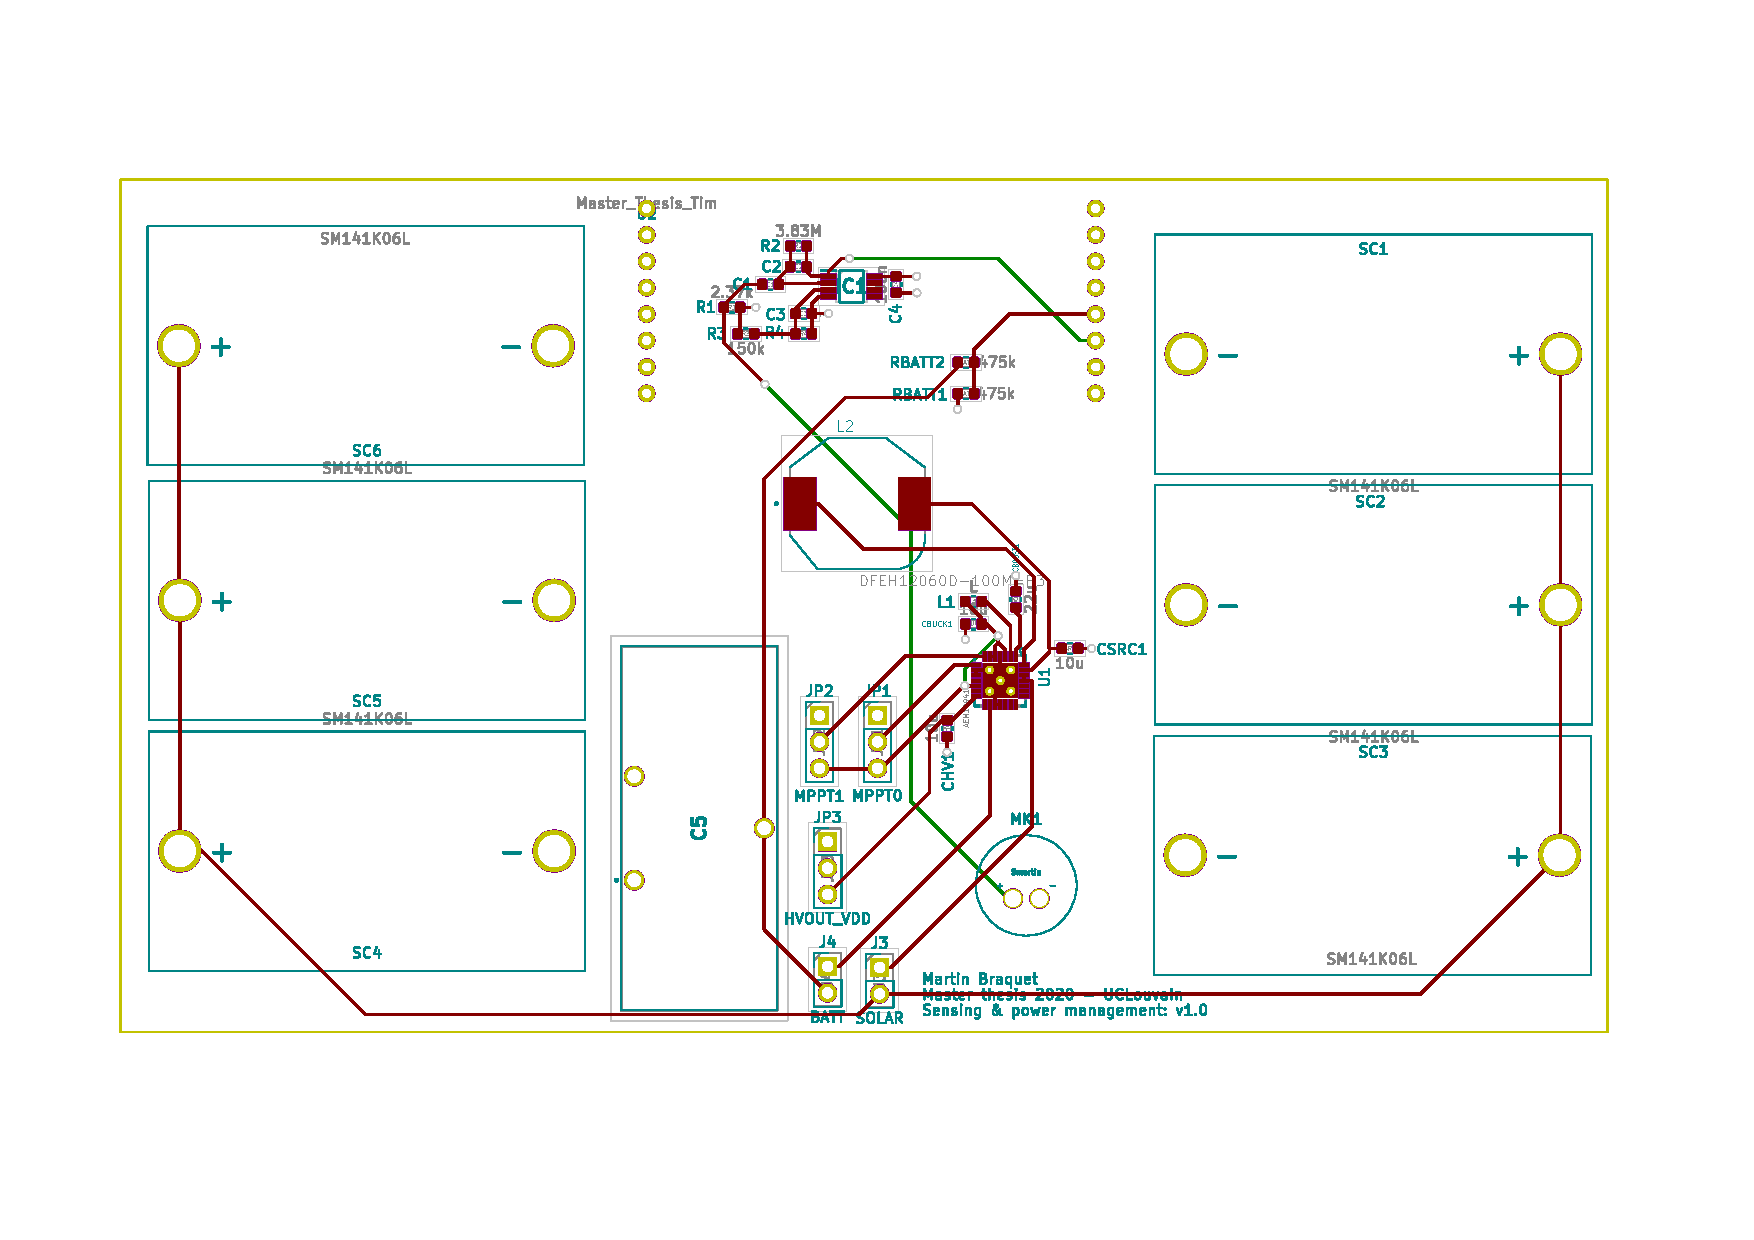
\includegraphics[width=0.9\textwidth]{sensing_PMU_layout.pdf}
    \caption{PCB layout}
    \label{fig:PCB_lay}
\end{figure}

\begin{figure}[H]
    \centering
    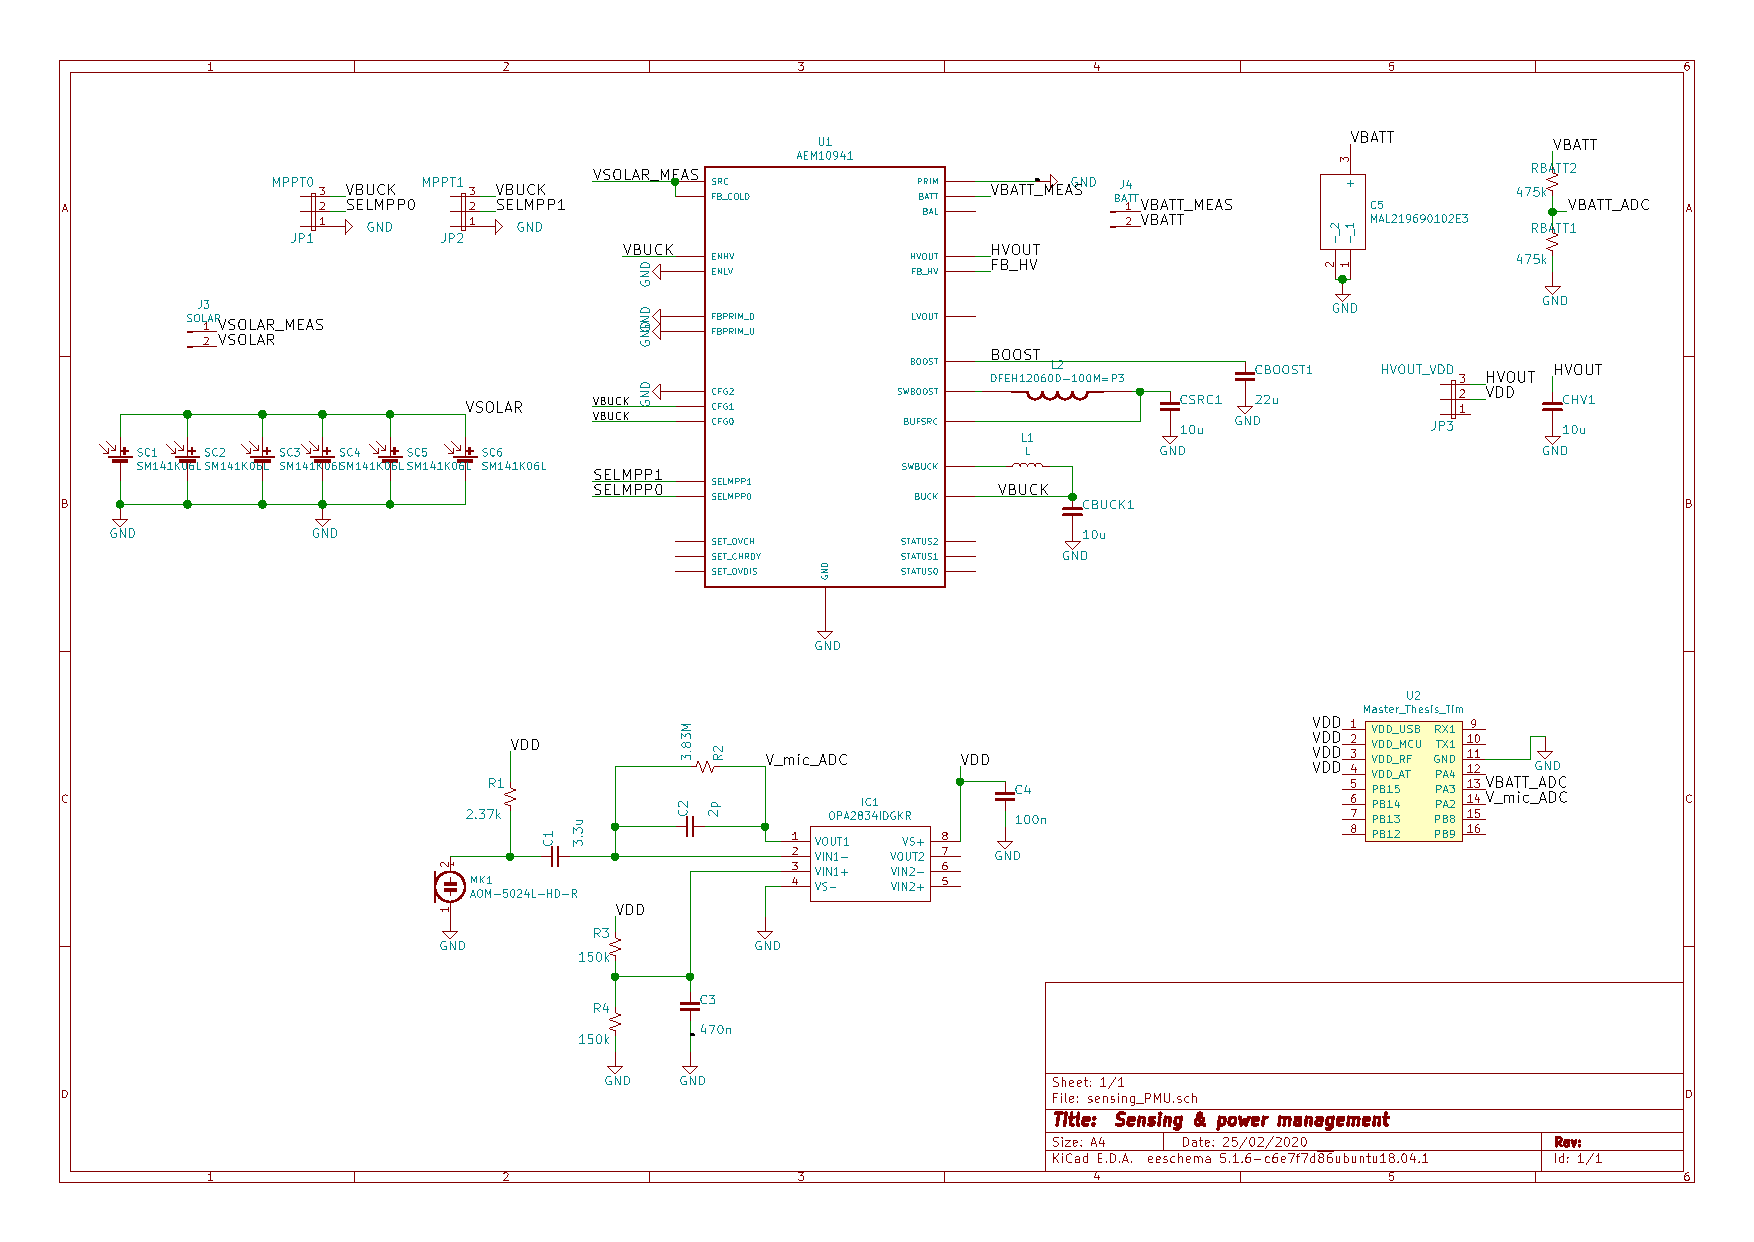
\includegraphics[width=\textwidth]{sensing_PMU_schematic.pdf}
    \caption{PCB schematics}
    \label{fig:PCB_sch}
\end{figure}


\bibliographystyle{unsrt}
\bibliography{biblio.bib}

% Back cover page
\backcoverpage

\end{document}
